%\documentclass{article}
\documentclass{book}
\usepackage{fullpage}

\newcommand{\textdir}{../..}

\newcommand{\tmpc}{\text{MPC}}
\newcommand{\treplay}{\text{replay}}
\newcommand{\tnew}{\text{new}}
\newcommand{\topt}{\text{opt}}
\newcommand{\wnew}{\vw_{\tnew}}


\setcounter{secnumdepth}{4}
\setcounter{tocdepth}{4}

\usepackage[utf8]{inputenc}
\usepackage[T1]{fontenc}

\usepackage[lines=3]{lettrine}
\usepackage{style/Zallman}
\usepackage[nopatch=footnote]{microtype}
\usepackage{fontawesome}
\usepackage{dsfont}
\usepackage{lmodern}
\usepackage{anyfontsize}
\usepackage{verbatim}
\usepackage{pifont}

\usepackage{quoting}
\usepackage{xcolor}

\usepackage{url}

\usepackage{tcolorbox}
\usepackage{booktabs,array}
\usepackage{makecell}
\usepackage{multirow}
\usepackage{tikz}
\usetikzlibrary{shapes.geometric,positioning}
\usepackage{pgfornament}


\usepackage[frozencache,cachedir=minted-output]{minted}

\usepackage{amsfonts,amssymb,amsmath}
\usepackage[noabbrev,nameinlink,capitalise,compress]{cleveref}
\usepackage{mathtools}
\usepackage{bm}
\usepackage{mathabx}
\usepackage{thmtools,thm-restate}
\usepackage{resizegather}
\usepackage{nicefrac}
\usepackage{xfrac}

\usepackage{enumitem}
\usepackage{setspace}
\usepackage{regexpatch}

\newcommand{\optimality}{{\mathcal O}}
\newcommand{\voptimality}{{\mathcal O}}
\newcommand{\penv}{p_{\text{env}}}
\newcommand{\done}{\text{done}}
\newcommand{\stopgrad}{\text{sg}}
%\newcommand{\snr}{\text{SNR}_{\infparams}}
\newcommand{\snr}{R}
\newcommand{\Jac}{\text{Jac}}
\newcommand{\icdf}{\text{icdf}}

\newcommand{\missing}{\text{mis}}
\newcommand{\observed}{\text{obs}}

\newcommand{\hmu}{\vh_{\vmu}}
\newcommand{\hsigma}{\vh_{\vSigma}}

\newcommand{\low}{\text{low}}
\newcommand{\high}{\text{high}}

\def\ceil#1{\lceil #1 \rceil}
\def\floor#1{\lfloor #1 \rfloor}
\def\1{\bm{1}}

\def\eps{{\epsilon}}

\newcommand{\Lsimple}{L_{\text{simple}}}
\newcommand{\oalpha}{\overline{\alpha}}

\newcommand{\env}{\calE}

\newcommand{\flowvx}{\vx}
\newcommand{\flowx}{x}
\newcommand{\flowvu}{\vu}
\newcommand{\flowu}{u}

\newcommand{\todokevin}[1]{{\color{green}{TODO(kevin):#1}}}
\newcommand{\balaji}[1]{{\color{red}{TODO(balaji):#1}}}
\newcommand{\notes}[1]{{\color{red}{#1}}}
\newcommand{\vcoupling}{\hat{\mathbf{f}}}
\newcommand{\coupling}{\hat{f}}
\newcommand{\scalarbijection}{h}
% KL divergence
\newcommand{\kl}[2]{D_{\mathrm{KL}}\left[\,#1\,\|\,#2\,\right]}
% Densities
\newcommand{\createDensityWithSub}[2]{{#1}_{\mathrm{#2}}}
\newcommand{\pz}{\createDensityWithSub{p}{z}}
\newcommand{\pzprime}{\createDensityWithSub{p}{z'}}
\newcommand{\px}{\createDensityWithSub{p}{x}}


\newcommand{\fdyn}{f^{\text{dyn}}}
\newcommand{\fobs}{f^{\text{obs}}}
\newcommand{\freward}{f^{\text{R}}}

\newcommand{\ESS}{\text{ESS}}

% LDA
\newcommand{\Ntopics}{{N_z}}
\newcommand{\Nwords}{{N_w}}


%https://www.overleaf.com/learn/latex/Mathematical_fonts
%\prescript{\mathrm t}{}{A},

%https://tex.stackexchange.com/questions/121865/nameref-how-to-display-section-name-and-its-number
\newcommand*{\fullref}[1]{\hyperref[{#1}]{\cref{#1} (\nameref*{#1})}}
%\newcommand*{\fullref}[1]{\hyperref[{#1}]{\autoref*{#1} (\nameref*{#1})}}

\newcommand{\eat}[1]{}
\newcommand{\new}{\text{new}}

%https://tex.stackexchange.com/questions/246/when-should-i-use-input-vs-include
\newcommand{\myinclude}[1]{\include{#1}}
%\newcommand{\myinclude}[1]{\input{#1}} 

\mathchardef\mhyphen="2D % Define a "math hyphen"
\mathchardef\mdash="2D % Define a "math hyphen"

\newcommand{\ie}{\emph{i.e.}}
\newcommand{\condition}{\,|\,}
\newcommand{\eg}{\emph{e.g.}}
\newcommand{\bo}{\mathbf{o}}
\newcommand{\bx}{\mathbf{x}}
\newcommand{\by}{\mathbf{y}}
\newcommand{\bc}{\mathbf{c}}

\newcommand{\colvec}[1]{\ensuremath{\begin{pmatrix} #1 \end{pmatrix}}}
\newcommand{\myvec}[1]{\mathbf{#1}}
\newcommand{\myvecsym}[1]{\boldsymbol{#1}}
%\newcommand{\myvecsym}[1]{\bm{#1}}
\newcommand{\mytensor}[1]{\mathbf{\tilde{#1}}}

%\newcommand{\prior}[1]{\underline{#1}}
%\newcommand{\post}[1]{\overline{#1}}

%\newcommand\smileacc[1]{\overset{\adjustedaccent{\smallsmile}}{#1}}
%\newcommand\frownacc[1]{\overset{\adjustedaccent{\smallfrown}}{#1}}
%\newcommand\smileacc[1]{\overset{\smallsmile}{#1}}
%\newcommand\frownacc[1]{\overset{\smallfrown}{#1}}

%https://tex.stackexchange.com/questions/194798/change-vertical-space-in-overset


\makeatletter
\newcommand{\oset}[3][-0.3ex]{%
  \mathrel{\mathop{#3}\limits^{
    \vbox to#1{\kern-4\ex@
    \hbox{$\scriptstyle#2$}\vss}}}}
\makeatother
\newcommand\smileacc[1]{\oset{\smallsmile}{#1}}
\newcommand\frownacc[1]{\oset{\smallfrown}{#1}}

\newcommand{\priorDist}{\pi_0}
\newcommand{\prior}[1]{\smileacc{#1}}
\newcommand{\post}[1]{\frownacc{#1}}

\newcommand{\pseudox}{\tilde{\vx}}
\newcommand{\acqfn}{\alpha}
\newcommand{\mynew}{\mathrm{new}}
\newcommand{\myold}{\mathrm{old}}
\newcommand{\mymin}{\mathrm{min}}
\newcommand{\mymax}{\mathrm{max}}
\newcommand{\rnn}{\mathrm{rnn}}

\newcommand{\acceptance}{A}
\newcommand{\centered}[1]{{#1}_c}

\newcommand{\vmask}{\vs}
\newcommand{\mask}{s}

\newcommand{\vauxvar}{\vv}
\newcommand{\auxvar}{v}

\newcommand{\SSeff}{S_{\text{eff}}}
\newcommand{\SSmin}{S_{\text{min}}}

% Numbers
\newcommand{\vzero}{\myvecsym{0}}
\newcommand{\vone}{\myvecsym{1}}


% Greek https://www.latex-tutorial.com/symbols/greek-alphabet/
\newcommand{\valpha}{\myvecsym{\alpha}}
\newcommand{\vbeta}{\myvecsym{\beta}}
\newcommand{\vchi}{\myvecsym{\chi}}
\newcommand{\vdelta}{\myvecsym{\delta}}
\newcommand{\vDelta}{\myvecsym{\Delta}}
\newcommand{\vepsilon}{\myvecsym{\epsilon}}
\newcommand{\vzeta}{\myvecsym{\zeta}}
\newcommand{\vXi}{\myvecsym{\Xi}}
\newcommand{\vell}{\myvecsym{\ell}}
\newcommand{\veta}{\myvecsym{\eta}}
%\newcommand{\vEta}{\myvecsym{\Eta}}
\newcommand{\vgamma}{\myvecsym{\gamma}}
\newcommand{\vGamma}{\myvecsym{\Gamma}}
\newcommand{\vmu}{\myvecsym{\mu}}
\newcommand{\vmut}{\myvecsym{\tilde{\mu}}}
\newcommand{\vnu}{\myvecsym{\nu}}
\newcommand{\vkappa}{\myvecsym{\kappa}}
\newcommand{\vlambda}{\myvecsym{\lambda}}
\newcommand{\vLambda}{\myvecsym{\Lambda}}
\newcommand{\vLambdaBar}{\overline{\vLambda}}
%\newcommand{\vnu}{\myvecsym{\nu}}
\newcommand{\vomega}{\myvecsym{\omega}}
\newcommand{\vOmega}{\myvecsym{\Omega}}
\newcommand{\vphi}{\myvecsym{\phi}}
\newcommand{\vvarphi}{\myvecsym{\varphi}}
\newcommand{\vPhi}{\myvecsym{\Phi}}
\newcommand{\vpi}{\myvecsym{\pi}}
\newcommand{\vPi}{\myvecsym{\Pi}}
\newcommand{\vpsi}{\myvecsym{\psi}}
\newcommand{\vPsi}{\myvecsym{\Psi}}
\newcommand{\vrho}{\myvecsym{\rho}}
\newcommand{\vtheta}{\myvecsym{\theta}}
\newcommand{\vthetat}{\myvecsym{\tilde{\theta}}}
\newcommand{\vTheta}{\myvecsym{\Theta}}
\newcommand{\vsigma}{\myvecsym{\sigma}}
\newcommand{\vSigma}{\myvecsym{\Sigma}}
\newcommand{\vSigmat}{\myvecsym{\tilde{\Sigma}}}
\newcommand{\vsigmoid}{\vsigma}
\newcommand{\vtau}{\myvecsym{\tau}}
\newcommand{\vxi}{\myvecsym{\xi}}


% Lower Roman (Vectors)
\newcommand{\va}{\myvec{a}}
\newcommand{\vb}{\myvec{b}}
\newcommand{\vBt}{\myvec{\tilde{B}}}
\newcommand{\vc}{\myvec{c}}
\newcommand{\vct}{\myvec{\tilde{c}}}
\newcommand{\vd}{\myvec{d}}
\newcommand{\ve}{\myvec{e}}
\newcommand{\vf}{\myvec{f}}
\newcommand{\vg}{\myvec{g}}
\newcommand{\vh}{\myvec{h}}
%\newcommand{\myvh}{\myvec{h}}
\newcommand{\vi}{\myvec{i}}
\newcommand{\vj}{\myvec{j}}
\newcommand{\vk}{\myvec{k}}
\newcommand{\vl}{\myvec{l}}
\newcommand{\vm}{\myvec{m}}
\newcommand{\vn}{\myvec{n}}
\newcommand{\vo}{\myvec{o}}
\newcommand{\vp}{\myvec{p}}
\newcommand{\vq}{\myvec{q}}
\newcommand{\vr}{\myvec{r}}
\newcommand{\vs}{\myvec{s}}
\newcommand{\vt}{\myvec{t}}
\newcommand{\vu}{\myvec{u}}
\newcommand{\vv}{\myvec{v}}
\newcommand{\vw}{\myvec{w}}
\newcommand{\vws}{\vw_s}
\newcommand{\vwt}{\myvec{\tilde{w}}}
\newcommand{\vWt}{\myvec{\tilde{W}}}
\newcommand{\vwh}{\hat{\vw}}
\newcommand{\vx}{\myvec{x}}
%\newcommand{\vx}{\myvec{x}}
\newcommand{\vxt}{\myvec{\tilde{x}}}
\newcommand{\vy}{\myvec{y}}
\newcommand{\vyt}{\myvec{\tilde{y}}}
\newcommand{\vz}{\myvec{z}}
%\newcommand{\vzt}{\myvec{\tilde{z}}}


% Elements of vectors
\def\evalpha{{\alpha}}
\def\evbeta{{\beta}}
\def\evepsilon{{\epsilon}}
\def\evlambda{{\lambda}}
\def\evomega{{\omega}}
\def\evmu{{\mu}}
\def\evpsi{{\psi}}
\def\evsigma{{\sigma}}
\def\evtheta{{\theta}}
\def\eva{{a}}
\def\evb{{b}}
\def\evc{{c}}
\def\evd{{d}}
\def\eve{{e}}
\def\evf{{f}}
\def\evg{{g}}
\def\evh{{h}}
\def\evi{{i}}
\def\evj{{j}}
\def\evk{{k}}
\def\evl{{l}}
\def\evm{{m}}
\def\evn{{n}}
\def\evo{{o}}
\def\evp{{p}}
\def\evq{{q}}
\def\evr{{r}}
\def\evs{{s}}
\def\evt{{t}}
\def\evu{{u}}
\def\evv{{v}}
\def\evw{{w}}
\def\evx{{x}}
\def\evy{{y}}
\def\evz{{z}}

% Upper Roman (Matrices)
\newcommand{\vA}{\myvec{A}}
\newcommand{\vB}{\myvec{B}}
\newcommand{\vC}{\myvec{C}}
\newcommand{\vD}{\myvec{D}}
\newcommand{\vE}{\myvec{E}}
\newcommand{\vF}{\myvec{F}}
\newcommand{\vG}{\myvec{G}}
\newcommand{\vH}{\myvec{H}}
\newcommand{\vI}{\myvec{I}}
\newcommand{\vJ}{\myvec{J}}
\newcommand{\vK}{\myvec{K}}
\newcommand{\vL}{\myvec{L}}
\newcommand{\vM}{\myvec{M}}
\newcommand{\vMt}{\myvec{\tilde{M}}}
\newcommand{\vN}{\myvec{N}}
\newcommand{\vO}{\myvec{O}}
\newcommand{\vP}{\myvec{P}}
\newcommand{\vQ}{\myvec{Q}}
\newcommand{\vR}{\myvec{R}}
\newcommand{\vS}{\myvec{S}}
\newcommand{\vT}{\myvec{T}}
\newcommand{\vU}{\myvec{U}}
\newcommand{\vV}{\myvec{V}}
\newcommand{\vW}{\myvec{W}}
\newcommand{\vX}{\myvec{X}}
%\newcommand{\vXs}{\vX_{\vs}}
\newcommand{\vXs}{\vX_{s}}
\newcommand{\vXt}{\myvec{\tilde{X}}}
\newcommand{\vY}{\myvec{Y}}
\newcommand{\vZ}{\myvec{Z}}
\newcommand{\vZt}{\myvec{\tilde{Z}}}
\newcommand{\vzt}{\myvec{\tilde{z}}}


% Matrix
\def\mA{{\bm{A}}}
\def\mB{{\bm{B}}}
\def\mC{{\bm{C}}}
\def\mD{{\bm{D}}}
\def\mE{{\bm{E}}}
\def\mF{{\bm{F}}}
\def\mG{{\bm{G}}}
\def\mH{{\bm{H}}}
\def\mI{{\bm{I}}}
\def\mJ{{\bm{J}}}
\def\mK{{\bm{K}}}
\def\mL{{\bm{L}}}
\def\mM{{\bm{M}}}
\def\mN{{\bm{N}}}
\def\mO{{\bm{O}}}
\def\mP{{\bm{P}}}
\def\mQ{{\bm{Q}}}
\def\mR{{\bm{R}}}
\def\mS{{\bm{S}}}
\def\mT{{\bm{T}}}
\def\mU{{\bm{U}}}
\def\mV{{\bm{V}}}
\def\mW{{\bm{W}}}
\def\mX{{\bm{X}}}
\def\mY{{\bm{Y}}}
\def\mZ{{\bm{Z}}}
\def\mBeta{{\bm{\beta}}}
\def\mPhi{{\bm{\Phi}}}
\def\mLambda{{\bm{\Lambda}}}
\def\mSigma{{\bm{\Sigma}}}


% tensors
%\newcommand{\tX}{\mytensor{X}}
%\newcommand{\tY}{\mytensor{Y}}
%\newcommand{\tZ}{\mytensor{Z}}
%\newcommand{\tW}{\mytensor{W}}


% Tensor
\DeclareMathAlphabet{\mathsfit}{\encodingdefault}{\sfdefault}{m}{sl}
\SetMathAlphabet{\mathsfit}{bold}{\encodingdefault}{\sfdefault}{bx}{n}
\newcommand{\tens}[1]{\bm{\mathsfit{#1}}}
\def\tA{{\tens{A}}}
\def\tB{{\tens{B}}}
\def\tC{{\tens{C}}}
\def\tD{{\tens{D}}}
\def\tE{{\tens{E}}}
\def\tF{{\tens{F}}}
\def\tG{{\tens{G}}}
\def\tH{{\tens{H}}}
\def\tI{{\tens{I}}}
\def\tJ{{\tens{J}}}
\def\tK{{\tens{K}}}
\def\tL{{\tens{L}}}
\def\tM{{\tens{M}}}
\def\tN{{\tens{N}}}
\def\tO{{\tens{O}}}
\def\tP{{\tens{P}}}
\def\tQ{{\tens{Q}}}
\def\tR{{\tens{R}}}
\def\tS{{\tens{S}}}
\def\tT{{\tens{T}}}
\def\tU{{\tens{U}}}
\def\tV{{\tens{V}}}
\def\tW{{\tens{W}}}
\def\tX{{\tens{X}}}
\def\tY{{\tens{Y}}}
\def\tZ{{\tens{Z}}}


% Graph
\def\gA{{\mathcal{A}}}
\def\gB{{\mathcal{B}}}
\def\gC{{\mathcal{C}}}
\def\gD{{\mathcal{D}}}
\def\gE{{\mathcal{E}}}
\def\gF{{\mathcal{F}}}
\def\gG{{\mathcal{G}}}
\def\gH{{\mathcal{H}}}
\def\gI{{\mathcal{I}}}
\def\gJ{{\mathcal{J}}}
\def\gK{{\mathcal{K}}}
\def\gL{{\mathcal{L}}}
\def\gM{{\mathcal{M}}}
\def\gN{{\mathcal{N}}}
\def\gO{{\mathcal{O}}}
\def\gP{{\mathcal{P}}}
\def\gQ{{\mathcal{Q}}}
\def\gR{{\mathcal{R}}}
\def\gS{{\mathcal{S}}}
\def\gT{{\mathcal{T}}}
\def\gU{{\mathcal{U}}}
\def\gV{{\mathcal{V}}}
\def\gW{{\mathcal{W}}}
\def\gX{{\mathcal{X}}}
\def\gY{{\mathcal{Y}}}
\def\gZ{{\mathcal{Z}}}

% Sets
\def\sA{{\mathbb{A}}}
\def\sB{{\mathbb{B}}}
\def\sC{{\mathbb{C}}}
\def\sD{{\mathbb{D}}}
% Don't use a set called E, because this would be the same as our symbol
% for expectation.
\def\sF{{\mathbb{F}}}
\def\sG{{\mathbb{G}}}
\def\sH{{\mathbb{H}}}
\def\sI{{\mathbb{I}}}
\def\sJ{{\mathbb{J}}}
\def\sK{{\mathbb{K}}}
\def\sL{{\mathbb{L}}}
\def\sM{{\mathbb{M}}}
\def\sN{{\mathbb{N}}}
\def\sO{{\mathbb{O}}}
\def\sP{{\mathbb{P}}}
\def\sQ{{\mathbb{Q}}}
\def\sR{{\mathbb{R}}}
\def\sS{{\mathbb{S}}}
\def\sT{{\mathbb{T}}}
\def\sU{{\mathbb{U}}}
\def\sV{{\mathbb{V}}}
\def\sW{{\mathbb{W}}}
\def\sX{{\mathbb{X}}}
\def\sY{{\mathbb{Y}}}
\def\sZ{{\mathbb{Z}}}

% Entries of a matrix
\def\emLambda{{\Lambda}}
\def\emA{{A}}
\def\emB{{B}}
\def\emC{{C}}
\def\emD{{D}}
\def\emE{{E}}
\def\emF{{F}}
\def\emG{{G}}
\def\emH{{H}}
\def\emI{{I}}
\def\emJ{{J}}
\def\emK{{K}}
\def\emL{{L}}
\def\emM{{M}}
\def\emN{{N}}
\def\emO{{O}}
\def\emP{{P}}
\def\emQ{{Q}}
\def\emR{{R}}
\def\emS{{S}}
\def\emT{{T}}
\def\emU{{U}}
\def\emV{{V}}
\def\emW{{W}}
\def\emX{{X}}
\def\emY{{Y}}
\def\emZ{{Z}}
\def\emSigma{{\Sigma}}

% entries of a tensor
% Same font as tensor, without \bm wrapper
\newcommand{\etens}[1]{\mathsfit{#1}}
\def\etLambda{{\etens{\Lambda}}}
\def\etA{{\etens{A}}}
\def\etB{{\etens{B}}}
\def\etC{{\etens{C}}}
\def\etD{{\etens{D}}}
\def\etE{{\etens{E}}}
\def\etF{{\etens{F}}}
\def\etG{{\etens{G}}}
\def\etH{{\etens{H}}}
\def\etI{{\etens{I}}}
\def\etJ{{\etens{J}}}
\def\etK{{\etens{K}}}
\def\etL{{\etens{L}}}
\def\etM{{\etens{M}}}
\def\etN{{\etens{N}}}
\def\etO{{\etens{O}}}
\def\etP{{\etens{P}}}
\def\etQ{{\etens{Q}}}
\def\etR{{\etens{R}}}
\def\etS{{\etens{S}}}
\def\etT{{\etens{T}}}
\def\etU{{\etens{U}}}
\def\etV{{\etens{V}}}
\def\etW{{\etens{W}}}
\def\etX{{\etens{X}}}
\def\etY{{\etens{Y}}}
\def\etZ{{\etens{Z}}}


\newcommand{\bbI}{\mathbb{I}}
\newcommand{\bbL}{\mathbb{L}}
\newcommand{\bbM}{\mathbb{M}}
\newcommand{\bbP}{\mathbb{P}}
\newcommand{\bbQ}{\mathbb{Q}}
\newcommand{\bbS}{\mathbb{S}}



%\newcommand{\mymathcal}[1]{\pazocal{#1}}
\newcommand{\mymathcal}[1]{\mathcal{#1}}

\newcommand{\calA}{\mymathcal{A}}
\newcommand{\calB}{\mymathcal{B}}
\newcommand{\calC}{\mymathcal{C}}
\newcommand{\calD}{{\mymathcal{D}}}
\newcommand{\calDx}{\calD_x}
\newcommand{\calE}{\mymathcal{E}}
\newcommand{\cale}{{\cal e}}
\newcommand{\calF}{\mymathcal{F}}
\newcommand{\calG}{\mymathcal{G}}
\newcommand{\calH}{\mymathcal{H}}
\newcommand{\calHX}{{\calH}_X}
\newcommand{\calHy}{{\calH}_y}
\newcommand{\calI}{\mymathcal{I}}
\newcommand{\calJ}{\mymathcal{J}}
\newcommand{\calK}{\mymathcal{K}}
\newcommand{\calL}{\mymathcal{L}}
\newcommand{\calM}{\mymathcal{M}}
\newcommand{\calN}{\mymathcal{N}}
\newcommand{\caln}{{\cal n}}
\newcommand{\calNP}{\mymathcal{NP}}
\newcommand{\calO}{\mymathcal{O}}
\newcommand{\calMp}{\calM^+}
\newcommand{\calMm}{\calM^-}
\newcommand{\calMo}{\calM^o}
\newcommand{\Ctest}{C_*}
\newcommand{\calP}{\mymathcal{P}}
\newcommand{\calq}{{\cal q}}
\newcommand{\calQ}{\mymathcal{Q}}
\newcommand{\calR}{\mymathcal{R}}
\newcommand{\calS}{\mymathcal{S}}
\newcommand{\calSstar}{\calS_*}
\newcommand{\calT}{\mymathcal{T}}
\newcommand{\calU}{\mymathcal{U}}
\newcommand{\calV}{\mymathcal{V}}
\newcommand{\calW}{\mymathcal{W}}
\newcommand{\calv}{{\cal v}}
\newcommand{\calX}{\mymathcal{X}}
\newcommand{\calY}{\mymathcal{Y}}
\newcommand{\calZ}{\mymathcal{Z}}


%%%%%%%

\newcommand{\betadist}{\mathrm{Beta}}
\newcommand{\Betadist}{\mathrm{Beta}}
\newcommand{\bernoulli}{\mathrm{Ber}}
\newcommand{\Ber}{\mathrm{Ber}}
\newcommand{\BB}{\mathrm{BetaBinom}}
\newcommand{\Binom}{\mathrm{Bin}}
\newcommand{\BinoDist}{\mathrm{Bin}}
\newcommand{\NegBinom}{\mathrm{NegBinom}}
\newcommand{\binomdist}{\mathrm{Bin}}
%\newcommand{\cauchy}{\mathrm{Cauchy}}
\newcommand{\cauchy}{\mathcal{C}}
\newcommand{\Cauchy}{\cauchy}
\newcommand{\DE}{\mathrm{DE}}
\newcommand{\DP}{\mathrm{DP}}
\newcommand{\PYP}{\mathrm{PYP}}
\newcommand{\Dir}{\mathrm{Dir}}
%\newcommand{\discrete}{\mathrm{Discrete}}
\newcommand{\erlang}{\mathrm{Erlang}}
\newcommand{\expdist}{\mathrm{Expon}}
\newcommand{\expon}{\mathrm{Expon}}
\newcommand{\expfam}{\mathrm{Expfam}}
\newcommand{\Expfam}{\mathrm{Expfam}}
\newcommand{\gammadist}{\mathrm{Ga}}
\newcommand{\Ga}{\mathrm{Ga}}
\newcommand{\GDP}{\mathrm{GDP}}
\newcommand{\GP}{\mathrm{GP}}
\newcommand{\GEM}{\mathrm{GEM}}
\newcommand{\gauss}{\mathcal{N}}
\newcommand{\loggauss}{\mathcal{LN}}
\newcommand{\matrixgauss}{\mathcal{MN}}
\newcommand{\MNIW}{\mathrm{MNIW}}
\newcommand{\circulargauss}{\mathrm{vMF}}
\newcommand{\gausscan}{\mathcal{N}_c}
\newcommand{\geom}{\mathrm{Geom}}
%\newcommand{\halfCauchy}{\mathrm{HalfCauchy}}
\newcommand{\halfCauchy}{\mathcal{C}_+}
\newcommand{\HalfCauchy}{\halfCauchy}
\newcommand{\halfcauchy}{\halfCauchy}
\newcommand{\halfNormal}{\mathcal{N}_+}
%\newcommand{\halfNormal}{\mathrm{HalfNormal}}
\newcommand{\horseshoe}{\mathrm{HS}}
%\newcommand{\IG}{\mathrm{InvGam}}
\newcommand{\IG}{\mathrm{IG}}
\newcommand{\IGauss}{\mathrm{InvGauss}}
%\newcommand{\invchi}{\chi^{-2}}
\newcommand{\invchisq}{\chi^{-2}}
\newcommand{\IW}{\mathrm{IW}}
\newcommand{\Laplace}{\mathrm{Laplace}}
\newcommand{\laplace}{\mathrm{Laplace}} % Laplace distribution
\newcommand{\LKJ}{\mathrm{LKJ}}
\newcommand{\LKJchol}{\mathrm{LKJchol}}
\newcommand{\logisticdist}{\mathrm{Logistic}}
%\newcommand{\Mu}{\mathrm{Mu}}
\newcommand{\Mu}{\mathcal{M}}
\newcommand{\Multi}{\Mu}
\newcommand{\NIX}{NI\chi^2}
\newcommand{\NJ}{\mathrm{NJ}}
\newcommand{\GIX}{NI\chi^2}
\newcommand{\NIG}{\mathrm{NIG}}
\newcommand{\GIG}{\mathrm{NIG}}
\newcommand{\NIW}{\mathrm{NIW}}
\newcommand{\GIW}{\mathrm{NIW}}
\newcommand{\GT}{{\mathrm{GT}}}
%\newcommand{\MVNIW}{\mathrm{MVNIW}}
\newcommand{\MVNIW}{\mathrm{NIW}}
\newcommand{\NW}{\mathrm{NWI}}
\newcommand{\NWI}{\mathrm{NWI}}
%\newcommand{\MVNIG}{\mathrm{MVNIG}}
\newcommand{\MVNIG}{\mathrm{NIG}}
\newcommand{\NGdist}{\mathrm{NG}}
\newcommand{\prob}{p}
\newcommand{\Plaw}{\mathbb{P}}
\newcommand{\Poi}{\mathrm{Poi}}
%\newcommand{\softmax}{\calS}
\newcommand{\softmax}{\mathrm{softmax}}
%\newcommand{\softmax}{\vsigma}
\newcommand{\Student}{\mathcal{T}}
\newcommand{\student}{\mathcal{T}}
\newcommand{\unif}{\mathrm{Unif}}
\newcommand{\Unif}{\unif}
\newcommand{\uniform}{\unif}
\newcommand{\Wishart}{\mathrm{Wi}}
\newcommand{\Wi}{\mathrm{Wi}}
\newcommand{\poissondist}{\mathrm{Poisson}}
\newcommand{\dirichletdist}{\mathrm{Dir}}

\newcommand{\cat}{\mathrm{Cat}}
%\newcommand{\cat}{\Mu}
\newcommand{\Cat}{\cat}
\newcommand{\discrete}{\cat}
\newcommand{\Discrete}{\cat}

\newcommand{\attn}{\mathrm{Attn}}
\newcommand{\atten}{\attn}
\newcommand{\attnWeights}{\alpha}
\newcommand{\attenWeights}{\attnWeights}
\newcommand{\attnScore}{a}
\newcommand{\attenScore}{\attnScore}

\newcommand{\LOO}{\mathrm{LOO}}
%%%%%%%%%%%%%%%%%%%%%%%%%%%%%%%%%%%%%%%%%%%%%%%%


\newcommand{\cbar}{\overline{c}}
\newcommand{\vcbar}{\overline{\vc}}
\newcommand{\fbar}{\overline{f}}
\newcommand{\myhbar}{\overline{h}}
\newcommand{\xmybar}{\overline{x}}
\newcommand{\ybar}{\overline{y}}
\newcommand{\zbar}{\overline{z}}
\newcommand{\vAbar}{\overline{\vA}}
\newcommand{\vBbar}{\overline{\vB}}
\newcommand{\vCbar}{\overline{\vC}}
\newcommand{\vxbar}{\overline{\vx}}
\newcommand{\vXbar}{\overline{\vX}}
\newcommand{\vybar}{\overline{\vy}}
\newcommand{\vYbar}{\overline{\vY}}
\newcommand{\vzbar}{\overline{\vz}}
\newcommand{\vZbar}{\overline{\vZ}}
\newcommand{\xbar}{\overline{x}}
\newcommand{\wbar}{\overline{w}}
\newcommand{\Xbar}{\overline{X}}
\newcommand{\Ybar}{\overline{Y}}
\newcommand{\Gbar}{\overline{G}}
\newcommand{\Jbar}{\overline{J}}
\newcommand{\Lbar}{\overline{\ell}}
\newcommand{\Nbar}{\overline{N}}
%\newcommand{\Qbar}{\overline{Q}}
\newcommand{\Qbar}{\overline{Q}}
\newcommand{\Abar}{\overline{A}}
\newcommand{\Tbar}{\overline{T}}
\newcommand{\Sbar}{\overline{S}}
\newcommand{\vSbar}{\overline{\vS}}
\newcommand{\Rbar}{\overline{R}}

\newcommand{\vtaubar}{\overline{\vtau}}
\newcommand{\vtbar}{\overline{\vt}}
\newcommand{\vsbar}{\overline{\vs}}
\newcommand{\mubar}{\overline{\mu}}
\newcommand{\phibar}{\overline{\phi}}



\newcommand{\lr}{\eta}
\newcommand{\stepsize}{\lr}
\newcommand{\momentum}{\gamma}
\newcommand{\dummy}{\mathrm{dummy}}
\newcommand{\onehot}{\mathrm{one}\mhyphen\mathrm{hot}}
%\newcommand{\onehot}{\mathrm{one-hot}}
\newcommand{\encode}{\mathrm{enc}}
\newcommand{\decode}{\mathrm{dec}}
\newcommand{\mydigamma}{\psi}

\newcommand{\AEencoder}{f_e}
\newcommand{\AEdecoder}{f_d}
\newcommand{\encoder}{e}
\newcommand{\backcoder}{b}
\newcommand{\decoder}{d}
\newcommand{\marginal}{m}


%\newcommand{\Wgen}{\vW_{\mathrm{gen}}}
%\newcommand{\Wrec}{\vW_{\mathrm{rec}}}

%https://www.overleaf.com/learn/latex/Theorems_and_proofs

%https://tex.stackexchange.com/questions/45355/theorem-numbering-as-chapter-section-subsection-theorem-number
\newtheorem{thm}{Theorem}[section]
\newtheorem{lem}{Lemma}[section]
\newtheorem{cor}{Corollary}[section]
\newtheorem{defn}{Definition}[section]

%\newenvironment{mythm}{{\bf Theorem}}{}
%\newenvironment{myproof}{{\bf Proof}}{}


\newcommand{\eos}{\text{\em{eos}}\xspace}
%\newcommand{\eos}{\langle /s \rangle}
\newcommand{\bos}{\text{\em{bos}}\xspace}
%\newcommand{\bos}{\langle s \rangle}
\newcommand{\pad}{\mathrm{<pad>}}
\newcommand{\unk}{\mathrm{<unk>}}

\newcommand{\unknown}{\vz} % state of nature

% make qed symbol a solid square
%\renewcommand{\qed}{\mbox{$\hrulefill \blacksquare $}}

%http://jblevins.org/notes/latex#independence
\newcommand\independent{\protect\mathpalette{\protect\independenT}{\perp}} 
\def\independenT#1#2{\mathrel{\rlap{$#1#2$}\mkern2mu{#1#2}}}


%http://imaging.mrc-cbu.cam.ac.uk/statswiki/TexTips
\newcommand{\argmax}{\operatornamewithlimits{argmax}}
\newcommand{\argmin}{\operatornamewithlimits{argmin}}

%\DeclareMathOperator*{\argmax}{arg\,max}
%\DeclareMathOperator*{\argmin}{arg\,min}

%\DeclareMathOperator{\sign}{sign}
%\DeclareMathOperator{\Tr}{Tr}
\let\ab\allowbreak

\newcommand{\todo}[1]{\textbf{TODO: #1}}
\newcommand{\todol}[1]{\textcolor{blue}{\textbf{LL: #1}}}

\newcommand{\reconstruct}[1]{r({#1})}
\newcommand{\recon}{r}
\newcommand{\act}{\vz}
\newcommand{\actScalar}{z}
\newcommand{\actMat}{\vZ}
\newcommand{\preact}{\va}
\newcommand{\preactScalar}{a}
\newcommand{\preactMat}{\vA}
\newcommand{\erf}{\text{erf}}
\newcommand{\activation}{\varphi}
\newcommand{\vactivation}{\varphi}
%\newcommand{\activation}{\phi}
%\newcommand{\vactivation}{\vphi}
\newcommand{\choice}[2]{\left(\!\!\! \begin{array}{c} #1 \\ #2\end{array} \!\!\!\right)}
\newcommand{\half}{\frac{1}{2}}
\newcommand{\nicehalf}{\nicefrac{1}{2}}

\newcommand{\addeq}{\stackrel{c}{=}}
\newcommand{\pluseq}{\mathrel{+}=}
%\newcommand{\defeq}{\stackrel{\rm def}{=}}
\newcommand{\defeq}{\triangleq}
%http://tex.stackexchange.com/questions/163829/delta-equal-to-symbol
%\def\defeq{\mathrel{\ensurestackMath{\stackon[2pt]{=}{\scriptstyle\Delta}}}}

%\newcommand{\defeq}{:=}
%\newcommand{\consteq}{\stackrel{+}{=}}
\newcommand{\consteq}{\bumpeq}
%\newcommand{\real}{{\rm I\hspace{-0.2em}R}}
%\newcommand{\real}{\mathbb{R}}
\newcommand{\real}{\sR}
\newcommand{\simplex}{\mathbb{S}}
%\newcommand{\posreal}{\mathbb{R}_{>0}}
\newcommand{\posreal}{\mathbb{R}_{+}}
\newcommand{\realpos}{\posreal}
\newcommand{\nonnegreal}{\mathbb{R}_{\geq 0}}
\newcommand{\ints}{\mathbb{Z}}
%\newcommand{\natural}{\mathbb{N}}
\newcommand{\posint}{\ints_{+}} % https://proofwiki.org/wiki/Symbols:Z
\newcommand{\intpos}{\posint}
\newcommand{\posints}{\posint}
%\newcommand{\posint}{\ints_{>0}} % https://proofwiki.org/wiki/Symbols:Z
\newcommand{\nonnegint}{\ints_{\geq 0}}


\newcommand{\train}{\text{train}}
\newcommand{\test}{\text{test}}
\newcommand{\valid}{\text{valid}}
\newcommand{\meta}{\text{meta}}

\newcommand{\testNull}{\test_{\text{null}}}
\newcommand{\testObs}{\test_{\text{obs}}}
\newcommand{\testStat}{t}

%\newcommand{\indep}{\perp}
%\newcommand{\given}{\|}
\newcommand{\given}{|}
\newcommand{\indep}[2]{{#1} \perp {#2}}
\newcommand{\condindep}[3]{{#1} \perp {#2} \; | \; {#3}}
\newcommand{\condindepG}[3]{{#1} \perp_G {#2} | {#3}}
\newcommand{\condindepP}[3]{{#1} \perp_p {#2} | {#3}}
\newcommand{\depend}[2]{{#1} \not \perp {#2}}
\newcommand{\conddepend}[3]{{#1} \not \perp {#2} | {#3}}

%\newcommand{\trans}{\top}
%\newcommand{\trans}{\intercal}
\newcommand{\trans}{{\mkern-1.5mu\mathsf{T}}}
\newcommand{\transpose}[1]{{#1}^{\trans}}

\newcommand{\inv}[1]{{#1}^{-1}}

\newcommand{\ra}{\rightarrow}
\newcommand{\lra}{\leftrightarrow}
\newcommand{\Ra}{\Rightarrow}
%\newcommand{\rv}{r.v.}
\newcommand{\la}{\leftarrow}
\newcommand{\tr}{\mathrm{tr}}
\newcommand{\st}{\ \ \ \ \mathrm{s.t.} \ \ \ }
\newcommand{\myst}{\ \  \mathrm{s.t.} \ \ }
%\newcommand{\det}{\mathrm{det}}
\newcommand{\size}{\mathrm{size}}
\newcommand{\trace}{\mathrm{tr}}
\newcommand{\mle}{\mathrm{mle}}
\newcommand{\pooled}{\mathrm{pooled}}
\newcommand{\bayes}{\mathrm{bayes}}
\newcommand{\ols}{\mathrm{ols}}
\newcommand{\old}{\mathrm{old}}
\newcommand{\unb}{\mathrm{unb}}
\newcommand{\map}{\mathrm{map}}
\newcommand{\mml}{\mathrm{mml}}


\newcommand{\hparams}{\vxi}
\newcommand{\hparam}{\xi}
\newcommand{\varparams}{\vpsi}
%\newcommand{\varparams}{\vlambda}
\newcommand{\vparams}{\varparams}
\newcommand{\vparamsScalar}{\psi}
\newcommand{\vparamstheta}{\vparams_{\vtheta}}
\newcommand{\infparams}{\vphi}
\newcommand{\params}{\vtheta}
\newcommand{\param}{\theta}
\newcommand{\genparams}{\vtheta}
%\newcommand{\nparams}{{\ensuremath{N_{\theta}}\xspace}}
\newcommand{\nparams}{D}
\newcommand{\Nparams}{\nparams}
\newcommand{\nopt}{n}
\newcommand{\infnet}{f^\text{inf}_{\infparams}}
\newcommand{\gennet}{f^\text{gen}_{\genparams}}
\newcommand{\qinf}{q_{\infparams}}
\newcommand{\qinfgen}{q_{\infparams,\genparams}}
\newcommand{\qvar}{q_{\varparams}}
\newcommand{\qvarn}{q_{\varparams_n}}
\newcommand{\pgen}{p_{\params}}
\newcommand{\reparam}{g}
%\newcommand{\reparam}{\text{REPARAM}}

%\newcommand{\hvar}{\ell_{\vparams}}
%\newcommand{\hvarHat}{\hat{\ell}_{\vparams}}
%\newcommand{\hh}{\ell}
  
%\newcommand{\optvarSpace}{\mathcal{X}}
%\newcommand{\optspace}{\mathcal{X}}
%\newcommand{\optvar}{x}
%\newcommand{\optvars}{\vx}
%\newcommand{\optvarsMatrix}{\vX}
%\newcommand{\xdata}{\va}


\newcommand{\optvarSpace}{\Theta}
\newcommand{\optspace}{\Theta}
\newcommand{\optvar}{\theta}
\newcommand{\optvars}{\vtheta}
\newcommand{\optvarsScalar}{\theta}
\newcommand{\optvarsMatrix}{\vTheta}
\newcommand{\xdata}{\vx}

\newcommand{\doptvarSpace}{\calX}
\newcommand{\doptspace}{\doptvarSpace}
\newcommand{\doptvar}{x}
\newcommand{\doptvars}{\vx}

% feynman kac
\newcommand{\fkM}{M}
\newcommand{\fkMM}{\bbM}
\newcommand{\fkQQ}{\bbQ}
\newcommand{\fkPP}{\bbP}
\newcommand{\fkG}{G}
\newcommand{\fkL}{L}
\newcommand{\fkl}{l}
\newcommand{\fkernel}{\stackrel{\ra}{M}}
\newcommand{\bkernel}{\stackrel{\la}{L}}
\newcommand{\bkernelOpt}{\stackrel{\la}{M}}


% importance sampling
\newcommand{\targetDist}{\pi}
\newcommand{\targetDistSeq}{\overline{\pi}}
\newcommand{\targetUn}{\tilde{\gamma}}
\newcommand{\targetEmp}{\hat{\pi}}
\newcommand{\targetfn}{\varphi}
\newcommand{\targetFn}{\targetfn}
\newcommand{\weightsUn}{\tilde{w}}
\newcommand{\weightsNorm}{W}
\newcommand{\weightsInc}{\alpha}

\newcommand{\ancestors}{a}
\newcommand{\ancestor}{a}

\newcommand{\smcH}{\vz}
\newcommand{\smcV}{\vy}
\newcommand{\backwards}{L}
\newcommand{\forwards}{M}

\newcommand{\proposalDist}{q}
\newcommand{\proposal}{q}
\newcommand{\qproposal}{\proposal}


\newcommand{\pmodel}{p_{\vtheta}}
\newcommand{\ptrue}{p^*}
%\newcommand{\pemp}{p_{\text{data}}}
\newcommand{\pemp}{p_{\data}}
\newcommand{\qemp}{q_{\data}}
\newcommand{\ptrain}{p_{\mathrm{tr}}}
%\newcommand{\ptrain}{p_1}
\newcommand{\ptest}{p_{\mathrm{te}}}
%\newcommand{\ptest}{p_2}
\newcommand{\pdata}{\pemp}

\newcommand{\psource}{p}
\newcommand{\ptarget}{q}

%\newcommand{\priorz}{\pi}
%\newcommand{\pgen}{p_G}
%\newcommand{\pteacher}{p_t}
%\newcommand{\pstudent}{p_s}

\newcommand{\postloss}{\rho}

\newcommand{\IDAG}{IDAG\xspace}
\newcommand{\doPearl}{\mathrm{do}}
\newcommand{\ceffect}{\tau}
\newcommand{\ETT}{\text{ETT}}
\newcommand{\ATE}{\text{ATE}}
\newcommand{\CATE}{\text{CATE}}
\newcommand{\exog}{U}
\newcommand{\exogVal}{u}
\newcommand{\exogSet}{\calU}
\newcommand{\scm}{V}
\newcommand{\scmVal}{v}
\newcommand{\scmSet}{\calV}
\newcommand{\POM}{POM\xspace}


\newcommand{\outcome}{Y}
\newcommand{\outcomeVal}{y}
\newcommand{\joutcome}{\tilde{\vY}}
\newcommand{\poutcome}[1]{\outcome^{#1}} % Y_a potential outcome
\newcommand{\pout}[2]{\outcome^{#1}_{#2}} % Y_{a,i} action a, unit  i
\newcommand{\ptreat}[2]{\treatment^{#1}_{#2}} %X_{a,i} action a, unit  i


\newcommand{\covariate}{C}
\newcommand{\covariateVal}{c}
\newcommand{\forceTreatment}{F_A}
\newcommand{\treatment}{A}
\newcommand{\treatmentVal}{a}
\newcommand{\treatmentValv}{\va}
\newcommand{\observation}{Y}
\newcommand{\lconfounder}{U}
\newcommand{\lconfounderVal}{u}
\newcommand{\confounder}{X}
\newcommand{\confounderVal}{x}
\newcommand{\deconfounder}{S}
\newcommand{\deconfounderVal}{s}
\newcommand{\mediator}{M}
\newcommand{\mediatorVal}{m}
\newcommand{\instrument}{Z}
\newcommand{\instrumentVal}{z}
\newcommand{\instrumentValv}{\vz}

  

\newcommand{\dom}{\mathrm{dom}}
\newcommand{\bel}{\mathrm{bel}}
\newcommand{\dsep}{\mathrm{dsep}}
\newcommand{\sep}{\mathrm{sep}}
\newcommand{\entails}{\models}
\newcommand{\range}{\mathrm{range}}
\newcommand{\myspan}{\mathrm{span}}
\newcommand{\nullspace}{\mathrm{nullspace}}
\newcommand{\adj}{\mathrm{adj}}
%\newcommand{\pval}{\mathrm{p}-\mathrm{value}}

\newcommand{\pval}{\mathrm{pval}}
\newcommand{\pvalue}{p_v}

\newcommand{\chol}{\mathrm{chol}}
\newcommand{\supp}{\mathrm{supp}}

%\newcommand{\xrange}[1]{[#1]}  % for set, [n]
\newcommand{\xrange}[1]{\ensuremath{\{1,\ldots,#1\}}}  % for set, [n]


%\newcommand{\dim}{\mathrm{dim}}
\newcommand{\length}{\mathrm{T}}
\newcommand{\sinc}{\mathrm{sinc}}
\newcommand{\mse}{\mathrm{mse}}
%\newcommand{\pon}{\pi_0}
\newcommand{\poff}{p_0}
\newcommand{\pon}{p_1}
\newcommand{\lse}{\ensuremath{\mathrm{lse}}\xspace}
\newcommand{\soft}{\mathrm{SoftThreshold}}
\newcommand{\hard}{\mathrm{hard}}
\newcommand{\cond}{\mathrm{cond}}
\newcommand{\sign}{\mathrm{sign}}
\newcommand{\sgn}{\mathrm{sgn}}

\newcommand{\iid}{\ensuremath{\mathrm{iid}}\xspace}
\newcommand{\myiff}{\ensuremath{\mathrm{iff}}\xspace}
\newcommand{\pd}{\ensuremath{\mathrm{pd}}\xspace}
\newcommand{\psd}{\ensuremath{\mathrm{psd}}\xspace}
\newcommand{\pdf}{\ensuremath{\mathrm{pdf}}\xspace}
\newcommand{\cdf}{\ensuremath{\mathrm{cdf}}\xspace}
\newcommand{\pmf}{\ensuremath{\mathrm{pmf}}\xspace}
\newcommand{\RV}{\ensuremath{\mathrm{rv}}\xspace}
%\newcommand{\rv}{\ensuremath{\mathrm{rv}}\xspace}
\newcommand{\wrt}{\ensuremath{\mathrm{wrt}}\xspace}
\newcommand{\mywp}{\ensuremath{\mathrm{wp}}\xspace}
\newcommand{\RSS}{\ensuremath{\mathrm{RSS}}\xspace}
\newcommand{\MSE}{\ensuremath{\mathrm{MSE}}\xspace}
\newcommand{\RMS}{\ensuremath{\mathrm{RMS}}\xspace}
\newcommand{\RMSE}{\ensuremath{\mathrm{RMSE}}\xspace}
\newcommand{\mydof}{\ensuremath{\mathrm{dof}}\xspace}
\newcommand{\dof}{\mydof}

\newcommand{\matlab}{{\sc MATLAB}}
\newcommand{\PMTK}{{\sc PMTK}}


\DeclareMathOperator{\JS}{D_\mathbb{JS}}
\newcommand{\JSpq}[2]{\JS\left({#1}\middle\Vert{#2}\right)}
\newcommand{\JSpi}[2]{\JS_{\pi}\left({#1}\middle\Vert{#2}\right)}
\DeclareMathOperator{\KL}{D_\mathbb{KL}}
%\DeclareMathOperator{\KL}{\mathbb{KL}}
%\newcommand{\KLpq}[2]{\KL\left({#1}\middle\Vert{#2}\right)}
%\newcommand{\KLpq}[2]{D_{\mathbb{KL}}\left({#1}\middle\Vert{#2}\right)}
\newcommand{\KLpq}[2]{D_{\mathbb{KL}}\left({#1} \mrel{\|} {#2}\right)}
\newcommand{\chipq}[2]{\chi^2\left({#1}\middle\Vert{#2}\right)}
\DeclareMathOperator{\MI}{\mathbb{I}}
\newcommand{\MIxy}[2]{\MI\left({#1};{#2}\right)}
\newcommand{\MIxyz}[3]{\MI\left({#1};{#2}|{#3}\right)}
\DeclareMathOperator{\PMI}{\mathbb{PMI}}
\DeclareMathOperator{\PPMI}{\mathbb{PPMI}}
\DeclareMathOperator{\entropy}{\mathbb{H}}
\DeclareMathOperator{\TC}{\mathbb{TC}}
\newcommand{\entropyp}[1]{\entropy\left({#1}\right)}
\newcommand{\crossentropy}{\entropy_{ce}}
\newcommand{\entropypq}[2]{\crossentropy\left({#1}, {#2}\right)}
\newcommand{\CE}{\text{CrossEntropy}}
\newcommand{\INCE}{\MI_{\mathrm{NCE}}}
\DeclareMathOperator{\fdiv}{D_f}
\newcommand{\fdivpq}[2]{\fdiv\left({#1}\middle\Vert{#2}\right)}

\newcommand{\hatf}{\hat{f}}
\newcommand{\hatp}{\hat{p}}
\newcommand{\haty}{\hat{y}}
\newcommand{\const}{\mathrm{const}}
%\newcommand{\sigmoid}{\mathrm{sigm}}
%\newcommand{\sigmoid}{\bm{\sigma}}
\newcommand{\sigmoid}{\sigma}
%\newcommand{\sigmoid}{\varsigma}
\newcommand{\softplus}{\sigma_{+}}

\newcommand{\relu}{\ensuremath{\mathrm{ReLU}}\xspace}
\newcommand{\gelu}{\ensuremath{\mathrm{GELU}}\xspace}
\newcommand{\resnet}{ResNet}

\newcommand{\deltafn}[2]{\delta(#1=#2)}
\newcommand{\ind}[1]{\mathbb{I}\left({#1}\right)}
\newcommand{\Ind}[1]{\ind{#1}}
\newcommand{\etr}{\mathrm{etr}}
\newcommand{\xor}{\veebar}
\newcommand{\LTU}{\mathrm{LTU}}
\newcommand{\heaviside}{H}

%\newcommand{\fin}{\mathrm{fan}_{\mathrm{in}}}
%\newcommand{\fout}{\mathrm{fan}_{\mathrm{out}}}
%\newcommand{\favg}{\mathrm{fan}_{\mathrm{avg}}}

\newcommand{\fin}{n_{\mathrm{in}}}
\newcommand{\fout}{n_{\mathrm{out}}}
\newcommand{\favg}{n_{\mathrm{avg}}}


\newcommand{\fisher}{F}
\newcommand{\Fisher}{\fisher} 
\newcommand{\vFisher}{\vF}
\newcommand{\vfisher}{\vFisher}



\newcommand{\ip}[2]{\langle #1, #2 \rangle}
\newcommand{\vvec}{\mathrm{vec}}
\newcommand{\vvech}{\mathrm{vech}}
\newcommand{\E}{\mathbb{E}} % \E{f(x)}
\newcommand{\expectAngle}[1]{\langle #1 \rangle} % \expectAngle{f(x)}
\newcommand{\expect}[1]{\mathbb{E}\left[{#1}\right]} %\expect{f(x)}
\newcommand{\expectQ}[2]{\mathbb{E}_{{#2}}\left[ {#1} \right]} %\expectAngle{f(x)}{p(x)}
%\newcommand{\Var}{\mathrm{Var}}
%\newcommand{\var}[1]{\mathrm{var}\left[{#1}\right]}
\newcommand{\Var}{\mathbb{V}}
\newcommand{\var}[1]{\mathbb{V}\left[ {#1}\right]}
\newcommand{\varQ}[2]{\mathbb{V}_{{#2}}\left[ {#1}\right]}
\newcommand{\std}[1]{\mathrm{std}\left [{#1}\right]}
\newcommand{\stderr}{\mathrm{se}}
\newcommand{\cov}[1]{\mathrm{Cov}\left[ {#1}\right] }
\newcommand{\covQ}[2]{\mathrm{Cov}_{{#2}}\left[ {#1}\right] }
\newcommand{\corr}[1]{\mathrm{corr}\left[ {#1}\right]}
\newcommand{\mymode}[1]{\mathrm{mode}\left[ {#1}\right]}
\newcommand{\median}[1]{\mathrm{median}\left[ {#1}\right]}


\newcommand{\sech}{\mathrm{sech}}
%\newcommand{\cosh}{\mathrm{cosh}}
\newcommand{\kurt}{\mathrm{kurt}}
\newcommand{\proj}{\mathrm{proj}}
\newcommand{\prox}{\mathrm{prox}}
\newcommand{\proxop}[2]{\prox_{#1}(#2)} % proxop{f}{v}
\newcommand{\proxopp}[3]{\prox_{#1,#2}(#3)} % proxop{f}{V}{v}
%\newcommand{\moreau}[2]{M_{#1}(#2)} % M{f}{v}
\newcommand{\myskew}{\mathrm{skew}}
\newcommand{\rank}{\mathrm{rank}}
\newcommand{\diag}{\mathrm{diag}}
\newcommand{\blkdiag}{\mathrm{blkdiag}}
\newcommand{\bias}{\mathrm{bias}}
\newcommand{\union}{\cup}
\newcommand{\intersect}{\cap}



%%%%%%%%%%%%%%%%%%%%%%%%%%%%%%%%%%%%%%%%%%%%%%%%



\newcommand{\vxtest}{\myvec{x}_*}
\newcommand{\ftrue}{f_{true}}
\newcommand{\myprec}{\mathrm{prec}}
\newcommand{\precw}{\lambda_{w}} % precision of weights (alpha)
\newcommand{\precy}{\lambda_{y}} % precision of y (beta)

\newcommand{\htilde}{\tilde{h}}
\newcommand{\vhtilde}{\tilde{\vh}}
\newcommand{\Dtilde}{\tilde{D}}
\newcommand{\Ftilde}{\tilde{F}}
\newcommand{\wtilde}{\tilde{w}}
\newcommand{\ptilde}{\tilde{p}}
\newcommand{\qtilde}{\tilde{q}}
\newcommand{\pstar}{p^*}
\newcommand{\xtilde}{\tilde{x}}
\newcommand{\Xtilde}{\tilde{X}}
\newcommand{\ytilde}{\tilde{y}}
\newcommand{\ym}{y^{-}}
\newcommand{\Ytilde}{\tilde{Y}}
\newcommand{\vxtilde}{\tilde{\vx}}
\newcommand{\vytilde}{\tilde{\vy}}
\newcommand{\ztilde}{\tilde{\z}}
\newcommand{\vthetaMAP}{\hat{\vtheta}_{MAP}}
\newcommand{\vthetaS}{\vtheta^{(s)}}
\newcommand{\vthetahat}{\hat{\vtheta}}
\newcommand{\thetahat}{\hat{\theta}}
\newcommand{\thetabar}{\overline{\theta}}
\newcommand{\thetastar}{\theta^*}
\newcommand{\vthetastar}{\vtheta^*}
\newcommand{\vthetabar}{\overline{\vtheta}}
\newcommand{\pibar}{\overline{\pi}}
\newcommand{\vpibar}{\overline{\vpi}}


% GPs
\newcommand{\kernelfn}{\mathcal{K}}
\newcommand{\kernelGauss}{\kernelfn_{\text{gauss}}}
\newcommand{\kernelfnShadow}{\mathcal{H}}
\newcommand{\kernelProfile}{k}
%\newcommand{\kernel}{\kappa}
%\newcommand{\meanfn}{\mu}
\newcommand{\meanfn}{m}




\newcommand{\nodes}{\calV}

\newcommand{\assign}{\leftarrow}

\newcommand{\dist}{\mathrm{dist}}
\newcommand{\class}{\mathrm{class}}
\newcommand{\NN}{\mathrm{NN}}

%\newcommand{\mya}{\mbox{a}}
%\newcommand{\myat}{\alpha_{t|t-1}}
\newcommand{\AIC}{\mathrm{AIC}}
\newcommand{\BIC}{\mathrm{BIC}}
\newcommand{\score}{\mathrm{score}}

\newcommand{\similarity}{\mathrm{sim}}

\newcommand{\model}{\calM}

\newcommand{\deriv}[2]{\frac{d {#1}}{d {#2}}}
\newcommand{\pderiv}[2]{\frac{\partial {#1}}{\partial {#2}}}

\newcommand{\sigmaSqMle}{\sigma^2_{\mle}}
\newcommand{\sigmaSqUnb}{\sigma^2_{\unb}}

%\newcommand{\mydesc}[2]{\textbf{#1}: #2}
\newcommand{\itemheader}[1]{\textbf{#1}.}

\newcommand{\DGM}{DPGM\xspace}
\newcommand{\UGM}{UPGM\xspace}
\newcommand{\PGM}{PGM\xspace}

\newcommand{\DGMs}{DPGMs\xspace}
\newcommand{\UGMs}{UPGMs\xspace}
\newcommand{\PGMs}{PGMs \xspace}

\newcommand{\iter}{t}
\newcommand{\niter}{T}
\newcommand{\predfn}{f}


\newcommand{\hyp}{h}
\newcommand{\hypspace}{\mathcal{H}}

  
%\newcommand{\ptran}{p_T}    % MDP transition model
\newcommand{\ptran}{p_S}    % MDP transition model
\newcommand{\preward}{p_R}    % MDP reward model
\newcommand{\policy}{\pi}
%\newcommand{\policy}{\Pi}
\newcommand{\policydet}{\mu_{\vtheta}}
\newcommand{\behavior}{\pi_b}
\newcommand{\policyexp}{\policy_{\mathrm{exp}}}
\newcommand{\traj}{\vtau}
\newcommand{\return}{G}
%\newcommand{\return}{R^{\ra}}
\newcommand{\initdist}{p_0}
%\newcommand{\initdist}{\mu_0}

\newcommand{\statmeasure}{\rho}
\newcommand{\statmeasuredet}{\rho_{\policydet}}

\newcommand{\ttraj}{\text{traj}}
\newcommand{\ttrue}{\text{true}}
\newcommand{\tsteps}{\text{steps}}
\newcommand{\tinit}{\text{init}}
\newcommand{\tpg}{\text{pol}}
\newcommand{\tpol}{\text{pol}}
\newcommand{\thorizon}{\text{maxlen}}
\newcommand{\tenv}{\text{env}}
\newcommand{\timag}{\text{imag}}
\newcommand{\tmodel}{\text{model}}
\newcommand{\ttot}{\text{total}}
\newcommand{\Mtrue}{M_{\text{env}}}
%\newcommand{\Mtrue}{M^*}
\newcommand{\Mest}{\hat{M}}
\newcommand{\MVE}{\hat{M}_{\text{VE}}}


\newcommand{\ttrace}{\text{trace}}
\newcommand{\tref}{\text{ref}}
\newcommand{\policyref}{\pi_{\tref}}

%\newcommand{\statdist}{p^{\infty}}
\newcommand{\statdist}{p^{\gamma}}
\newcommand{\statdistpol}{\statdist_{\policy}}
\newcommand{\statdistpolk}{\statdist_{\policy_k}}
\newcommand{\statdistpolki}{\statdist_{\policy_{k-i}}}
\newcommand{\statdistpolref}{\statdist_{\policyref}}
\newcommand{\statdistpolapprox}{\statdist_{\polapprox}}
\newcommand{\statdistbehave}{\statdist_{\behavior}}
\newcommand{\statdistdet}{\statdist_{\policydet}}
\newcommand{\policydist}{p_{\policy}^t}
\newcommand{\statdistpolexp}{\statdist_{\policyexp}}

\newcommand{\Vapprox}{V_{\vw}}
\newcommand{\Qapprox}{Q_{\vw}}
\newcommand{\Vpol}{V_{\policy}}
\newcommand{\Vpolapprox}{V_{\polapprox}}
\newcommand{\Vpoll}{V_{\policy'}}
\newcommand{\Vpolopt}{V_{\polopt}}
\newcommand{\Vopt}{V_{*}}
\newcommand{\Vdet}{V_{\policydet}}
\newcommand{\Qpol}{Q_{\policy}}
\newcommand{\Qpolapprox}{Q_{\polapprox}}
\newcommand{\Qopt}{Q_{*}}
\newcommand{\Qdet}{Q_{\policydet}}
\newcommand{\advantage}{A}
\newcommand{\Apol}{A_{\policy}}
\newcommand{\Apolapprox}{A_{\polappxorox}}
\newcommand{\Aopt}{A_{*}}
\newcommand{\Aapprox}{A_{\vw}}
\newcommand{\polopt}{\policy_{*}}
\newcommand{\polapprox}{\policy_{\vtheta}}
\newcommand{\polfn}{\policy_{\vtheta}}
\newcommand{\regret}{l}    % per-step regret
\newcommand{\totalRegret}{L}    % total regret
\newcommand{\estP}{\hat{P}}    % estimated transition
\newcommand{\estR}{\hat{R}}    % estimated reward
\newcommand{\optR}{\tilde{R}}    % optimistic reward
\newcommand{\estQ}{\hat{Q}}    % estmated Q-function
\newcommand{\estV}{\hat{V}}    % estimated V-function
\newcommand{\trueQ}[1]{Q_{#1}}    % true Q-function
\newcommand{\trueV}[1]{V_{#1}}    % true V-function
\newcommand{\bstate}{\vb}    % belief state
\newcommand{\polval}{J}    % policy value
\newcommand{\polvallin}{L}    % policy value first order term
\newcommand{\polvalest}{\hat{\polval}}    % estimated policy value
\newcommand{\polvaldm}{\polvalest_{\mathrm{DM}}}    % DM policy value
\newcommand{\polvalis}{\polvalest_{\mathrm{IS}}}    % basic IS policy value estimate
\newcommand{\polvalpdis}{\polvalest_{\mathrm{PDIS}}}    % per-decision IS policy value estimate
\newcommand{\polvaldr}{\polvalest_{\mathrm{DR}}}    % DR policy value
\newcommand{\polvalbeh}{\polval_b}    % policy value under behavior distribution
\newcommand{\policytgt}{\policy}    % target policy
\newcommand{\policybeh}{\policy_b}    % behavior policy
\newcommand{\estPolicybeh}{\hat{\policy}_b}    % estimated behavior policy
\newcommand{\psiRatio}{\rho}    % per-step importance ratio
\newcommand{\estPsiRatio}{\hat{\rho}}     % estimated per-step importance ratio
\newcommand{\statdistdata}{p_{\data}}    % off-policy data distribution over (s,a)
\newcommand{\statdistcorr}{\zeta}    % off-policy data distribution correction factor

\newcommand{\targetV}{q}
%\newcommand{\targetV}{\text{TargetV}}
\newcommand{\TargetV}{\targetV}
\newcommand{\estimatorE}{\hat{\Theta}}
\newcommand{\estimator}{\delta}
\newcommand{\SamplingDist}{\mathrm{SamplingDist}}

\newcommand{\Linf}{\ensuremath{\ell_{\infty}}\xspace}
\newcommand{\Lone}{\ensuremath{\ell_1}\xspace}
\newcommand{\Ltwo}{\ensuremath{\ell_2}\xspace}

\newcommand{\penaltyfn}{\phi}
\newcommand{\nconstr}{m}
\newcommand{\constrSet}{\mathcal{C}}
\newcommand{\ineqconstrSet}{\mathcal{I}}
\newcommand{\eqconstrSet}{\mathcal{E}}
\newcommand{\constr}{c}
\newcommand{\constrs}{\vc}
%\newcommand{\eqconstr}{c^{=}}
%\newcommand{\ineqconstr}{c^{\geq}}
\newcommand{\eqconstr}{h}
\newcommand{\ineqconstr}{g}
\newcommand{\eqconstrs}{\vh}
\newcommand{\ineqconstrs}{\vg}


\newcommand{\costfn}{\loss}
\newcommand{\costfnStoch}{\tilde{\loss}}
\newcommand{\stochfn}{\costfnStoch}
\newcommand{\costfnSmooth}{\loss_s}
\newcommand{\costfnRough}{\loss_r}
\newcommand{\lagrange}{L}
\newcommand{\taylor}{\mathcal{T}}
\newcommand{\paramspace}{\Theta}
\newcommand{\feasible}{\mathcal{C}}
\newcommand{\upperbound}{U}



\newcommand{\sample}{\vz}
\newcommand{\sampleScalar}{z}
\newcommand{\sampledist}{q}

\newcommand{\noise}{\vepsilon}
\newcommand{\noisedist}{q_0}
\newcommand{\baseline}{b}

% Discrete optimization
\newcommand{\scorefn}{f} % reward
\newcommand{\states}{\vs}
\newcommand{\state}{s}
\newcommand{\statespace}{\mathcal{S}}

 %https://tex.stackexchange.com/questions/468409/how-do-i-reproduce-a-calligraphic-z-that-looks-like-an-l-from-a-text-by-abramo/468438
%\newcommand{\loglik}{\textcursive{L}}
%\newcommand{\loglik}{\mathrm{LL}}
\newcommand{\loglik}{\ell}
%\newcommand{\loglik}{LL}
\newcommand{\lik}{\loglik}

\newcommand{\loss}{\calL}
\newcommand{\NLL}{\ensuremath{\mathrm{NLL}}\xspace}
\newcommand{\NLLN}{\ensuremath{\mathrm{NLLN}}\xspace}
\newcommand{\PNLL}{\ensuremath{\mathrm{PNLL}}\xspace}
\newcommand{\cost}{c}


%\newcommand{\elbo}{\mathscr{E}}
%\newcommand{\elbo}{\mathcal{E}}
%\newcommand{\elbo}{\mathscr{L}}
\newcommand{\elbo}{\text{\L}}
\newcommand{\helbo}{\hat{\elbo}}
\newcommand{\telbo}{\elbo}
%\newcommand{\elbo}{\text{ELBO}}
%\newcommand{\elbow}{\elbo_{\vtheta,\vphi}}
\newcommand{\elbow}[1]{\elbo(\vtheta,\vphi|#1)}
%\newcommand{\elbo}{\mathfrak{E}}
\newcommand{\ELBO}{\elbo}
\newcommand{\nelbo}{\mathrm{NELBO}}
\newcommand{\ielbo}{\tilde{\end{description}\elbo}}
\newcommand{\EUBO}{\text{EUBO}}
\newcommand{\CUBO}{\text{CUBO}}

\newcommand{\EU}{\mathrm{EU}}
\newcommand{\MEU}{\mathrm{MEU}}

\newcommand{\utilityfn}{U} % U(truth, pred)
%\newcommand{\lossfn}{\ell} % \lossfn(truth, pred)
\newcommand{\lossfn}{\ell} % \lossfn(truth, pred)
\newcommand{\squaredloss}{\ensuremath{\ell_{2}}}
\newcommand{\binaryloss}{\ensuremath{\ell_{01}}}
\newcommand{\logloss}{\ensuremath{\ell_{ll}}}
\newcommand{\hingeloss}{\ensuremath{\ell_{\mathrm{hinge}}}}
\newcommand{\huberloss}{\ensuremath{\ell_{\mathrm{huber}}}}
%\newcommand{\celoss}{\ensuremath{\ell_{\mathrm{ce}}}}


\newcommand{\ftarget}{f^*}
\newcommand{\fprior}{f^{\mathrm{prior}}}
\newcommand{\history}{\vh}
\newcommand{\data}{\calD}
\newcommand{\dataAug}{\calD_{\mathrm{aug}}}
\newcommand{\dataTrain}{\calD_{\mathrm{train}}}
\newcommand{\dataTest}{\calD_{\mathrm{test}}}
\newcommand{\dataValid}{\calD_{\mathrm{valid}}}
\newcommand{\dataPrior}{\calD_{\mathrm{prior}}}
\newcommand{\dataMeta}{\calD_{\mathrm{meta}}}
\newcommand{\dataExp}{\calD_{\mathrm{exp}}}
\newcommand{\dataAll}{\calD_{\mathrm{all}}}

%\newcommand{\N}{{\ensuremath{\tilde{N}}}}
\newcommand{\N}{N}
%\newcommand{\Ndata}{{N_{\mathrm{data}}\xspace}}
%\newcommand{\Ndata}{{N_{\mathcal{D}}\xspace}}
%\newcommand{\Ndata}{{N_{\calD}}}
\newcommand{\Ndata}{N}
\newcommand{\ndata}{\Ndata}

\newcommand{\timeInt}{n}
\newcommand{\timeTot}{m}

\newcommand{\futuredata}{\tilde{\calD}}
\newcommand{\algo}{\calA}
\newcommand{\fitAlgo}{\calF}
\newcommand{\predictAlgo}{\calP}
%\newcommand{\data}{D}
\newcommand{\err}{\mathrm{err}}
\newcommand{\logit}{\mathrm{logit}}

\newcommand{\errApprox}{\calE_{\mathrm{app}}(\calH)}
\newcommand{\errEst}{\calE_{\mathrm{est}}(\calH,N)}
\newcommand{\valrisk}{R^{\mathrm{val}}}
\newcommand{\cvrisk}{R^{\mathrm{cv}}}



\newcommand{\inputs}{\vu}
\newcommand{\vinputs}{\vu}
\newcommand{\features}{\vphi}
\newcommand{\vfeatures}{\vphi}
\newcommand{\pot}{\psi}
\newcommand{\word}{w}

\newcommand{\Nout}{C}

\newcommand{\Nc}{{N_c}}
\newcommand{\Nl}{{N_l}}
\newcommand{\No}{{N_o}}
\newcommand{\Nr}{{N_r}}
\newcommand{\Nu}{{N_u}}
\newcommand{\Nv}{{N_v}}
\newcommand{\Nx}{{N_x}}
\newcommand{\Ny}{{N_y}}
\newcommand{\Nz}{{N_z}}

\newcommand{\suffstat}{\mathcal{T}}
%\newcommand{\suffstat}{\mathbf{s}}
\newcommand{\suffstatScalar}{\suffstat}
%\newcommand{\suffstat}{\vt}
%\newcommand{\suffstat}{\vphi}

\newcommand{\Niter}{T}
\newcommand{\batch}{\mathcal{B}}
\newcommand{\Ndim}{D}
%\newcommand{\Nsamples}{n_s}
\newcommand{\Nsamples}{N_s}
\newcommand{\nsamples}{\Nsamples}
\newcommand{\Nlowdim}{L}
\newcommand{\Nlow}{\Nlowdim}
%\newcommand{\Nfolds}{K}
\newcommand{\Nclusters}{N_c}
%\newcommand{\Nnodes}{{|G|}}
%\newcommand{\Nedges}{E}
\newcommand{\Nnodes}{{N_G}}
\newcommand{\nnodes}{\Nnodes}
\newcommand{\nodei}{{i}}
\newcommand{\nodej}{{j}}
%\newcommand{\Nfuture}{\tilde{N}}
\newcommand{\Nfuture}{M}



%%%%%%%%%%%%%%
% SSM

\newcommand{\nsymbols}{N_y}
\newcommand{\Nstates}{K}
%\newcommand{\Nstates}{N_z}
\newcommand{\nstates}{\Nstates}
\newcommand{\nswitch}{N_m}

\newcommand{\dlatent}{m}
\newcommand{\dlatents}{\vm}
%\newcommand{\dlatent}{s}
%\newcommand{\dlatents}{\vs}

\newcommand{\hidden}{\vz}
\newcommand{\Hidden}{\vZ}
\newcommand{\hiddenScalar}{z}
\newcommand{\hiddenNode}{\hiddenScalar}
\newcommand{\latent}{\hiddenNode}
\newcommand{\obs}{\vy}
\newcommand{\obsHyp}{\tilde{\obs}}
\newcommand{\Obs}{\vY}
\newcommand{\obsScalar}{y}
\newcommand{\obsNode}{\obsScalar}



\newcommand{\hmmTrans}{\vA}
\newcommand{\hmmTransScalar}{A}
\newcommand{\hmmObs}{\vB}
\newcommand{\hmmObsScalar}{B}
\newcommand{\hmmInit}{\vpi}
\newcommand{\hmmInitScalar}{\pi}
\newcommand{\hmmMix}{\vw}
\newcommand{\hmmMixScalar}{w}

%\newcommand{\NlatentKF}{N_z}
%\newcommand{\NobsKF}{N_y}
\newcommand{\nhidden}{N_z}
\newcommand{\nobs}{N_y}
\newcommand{\ninputs}{N_u}
\newcommand{\nfeatures}{N_x}


\newcommand{\jac}{\text{Jac}}

\newcommand{\SSM}{State-space model}
\newcommand{\ssm}{state-space model}
\newcommand{\ssms}{state-space models}

\newcommand{\ldsTrans}{\vF}
\newcommand{\ldsObs}{\vH}
\newcommand{\ldsTransIn}{\vB}
\newcommand{\ldsObsIn}{\vD}
\newcommand{\ldsObsAR}{\vE}
\newcommand{\transCov}{\vQ}
\newcommand{\transCovExtra}{\tilde{\vQ}}
\newcommand{\transVar}{Q}
\newcommand{\transNoise}{\vq}
\newcommand{\transNoiseScalar}{q}
\newcommand{\obsCov}{\vR}
\newcommand{\obsCovExtra}{\tilde{\vR}}
\newcommand{\obsVar}{R}
\newcommand{\obsNoise}{\vr}
\newcommand{\obsNoiseScalar}{r}
\newcommand{\ldsTransBias}{\vb}
\newcommand{\ldsObsBias}{\vd}

\newcommand{\kalmanGain}{\vK}
%\newcommand{\rtsGain}{\vG}
\newcommand{\rtsGain}{\vJ}
  
%\newcommand{\fn}{\vf}
%\newcommand{\fnScalar}{f}
%\newcommand{\fnJac}{\vJ_{\vf}}

\newcommand{\fn}{\vg}
\newcommand{\fnScalar}{g}
\newcommand{\fnJac}{\vG}

\newcommand{\fnIn}{\vx}
\newcommand{\fnOut}{\vy}
\newcommand{\fnCov}{\vOmega}

\newcommand{\transFn}{\vf}
\newcommand{\transFnScalar}{f}
%\newcommand{\transFnJac}{\vJ_{\vf}}
\newcommand{\transFnJac}{\vF}
\newcommand{\obsFn}{\vh}
\newcommand{\obsFnScalar}{h}
%\newcommand{\obsFnJac}{\vJ_{\vh}}
\newcommand{\obsFnJac}{\vH}

\newcommand{\sigmaPointsFn}{\mathbf{SigmaPoints}}
%\newcommand{\unscentedFn}{\mathbf{UnscentedPredict}}
\newcommand{\unscentedFn}{\mathbf{UnscentedMoments}}
%\newcommand{\linearizeFn}{\mathbf{LinearizedPredict}}
\newcommand{\linearizeFn}{\mathbf{LinearizedMoments}}
%\newcommand{\affineFn}{\mathbf{AffineApprox}}
%\newcommand{\linearizeCondFn}{\mathbf{CondLinearizedPredict}}
\newcommand{\linearizeCondFn}{\mathbf{CondLinearizedMoments}}
\newcommand{\slrFn}{\mathbf{SLR}}
\newcommand{\gaussConditionFn}{\mathbf{GaussCondition}}
\newcommand{\gaussSoftConditionFn}{\mathbf{GaussSoftCondition}}
%\newcommand{\gaussSmoothFn}{\mathbf{GaussSmoothUpdate}}
\newcommand{\gaussSmoothFn}{\gaussSoftConditionFn}
%\newcommand{\gaussUpdateFn}{\mathbf{LinGaussUpdate}}
%\newcommand{\gaussPredictFn}{\mathbf{LinGaussPredict}}
\newcommand{\gaussMomentsFn}{\mathbf{GaussMoments}}
\newcommand{\condMomentsFn}{\mathbf{CondMoments}}
\newcommand{\IPLF}{\mathbf{IPLF}}
\newcommand{\IPLS}{\mathbf{IPLS}}
\newcommand{\IEKF}{\mathbf{IEKF}}
\newcommand{\IMMF}{\mathbf{GIPLF}}


%%%%%%%%%%%%%%%%%

%\newcommand{\ldacount}{N} % count of each word
%\newcommand{\hmmlda}{h} % hidden state of HMM in HMM-LDA model
%\newcommand{\Ntopics}{{K}}
%\newcommand{\Nwords}{{V}}
%\newcommand{\Nvocab}{{V}}

% graph terms
\newcommand{\Npastates}{{\ensuremath{N_{\pi}}}}
\newcommand{\nbd}{\mathrm{nbd}}
\newcommand{\nbr}{\mathrm{nbr}}
\newcommand{\anc}{\mathrm{anc}}
\newcommand{\desc}{\mathrm{desc}}
\newcommand{\pred}{\mathrm{pred}}
\newcommand{\mysucc}{\mathrm{suc}}
\newcommand{\nondesc}{\mathrm{nd}}
\newcommand{\pa}{\mathrm{pa}}
%\newcommand{\pa}{\pi}
\newcommand{\parent}{\mathrm{pa}}
\newcommand{\family}{\mathrm{fam}}
\newcommand{\copa}{\mathrm{copa}}
\newcommand{\ch}{\mathrm{ch}}
\newcommand{\mb}{\mathrm{mb}}
\newcommand{\connects}{\sim}
\newcommand{\nd}{\mathrm{nd}}
\newcommand{\bd}{\mathrm{bd}}
\newcommand{\cl}{\mathrm{cl}}

\DeclareMathOperator{\children}{Ch}
\DeclareMathOperator{\parents}{Pa}


\newcommand{\topK}{\mathrm{top}\mhyphen\mathrm{K}}
\newcommand{\MLE}{\mathrm{MLE}}


\newcommand{\be}{\begin{equation}}
\newcommand{\ee}{\end{equation}}
% for cormen.cls, we define
%\newcommand{\be}{\begin{eqnarray}}
%\newcommand{\ee}{\end{eqnarray}}
% NOTE that use of eqnarray causes issues with \label and \cref

\newcommand{\bea}{\begin{eqnarray}}
\newcommand{\eea}{\end{eqnarray}}
\newcommand{\beaa}{\begin{eqnarray*}}
\newcommand{\eeaa}{\end{eqnarray*}}
\newcommand{\ba}{\begin{align*}}
\newcommand{\ea}{\end{align*}}


%https://en.wikipedia.org/wiki/List_of_mathematical_symbols_by_subject
%\DeclareMathOperator{\dotstar}{\circ}
\DeclareMathOperator{\dotstar}{\odot}
\DeclareMathOperator{\kron}{\otimes}

\DeclareMathOperator{\convolve}{\circledast}
\DeclareMathOperator{\conv}{\convolve}
\DeclareMathOperator{\xcorr}{\ast}
%\DeclareMathOperator{\xcorr}{\times}

\newcommand{\imcol}{\mathrm{I2C}}
\newcommand{\reshape}{\mathrm{T2M}}
\newcommand{\unreshape}{\mathrm{M2T}}

\newcommand{\eigmax}{\lambda_{\mathrm{max}}}
\newcommand{\eigmin}{\lambda_{\mathrm{min}}}

%\newcommand{\figdir}{../figures}
\newcommand{\dldir}{\figdir}


\newcommand{\figgen}[1]{Generated by #1} % Example usage: \figgen{\notenook{foo}}


%% \iftoggle{draft}
%% { % draft mode
%% \newcommand{\figgen}[1]{Generated by #1} % Example usage: \figgen{\pycode{foo}}
%% }
%% { % non_draft mode
%% %  \newcommand{\figgen}[1]{Generated by \href{https://code.probml.ai/\bookname/\thefigure}{code.probml.ai/\bookname/\thefigure}}
%%   \newcommand{\figgen}[1]{Generated by \href{https://code.probml.ai/\bookname/\thefigure}{#1}}
%% }
%https://github.com/probml/pyprobml/blob/master/notebooks/book2/02/bayes_change_of_var.ipynb


\newcommand{\figbased}[1]{Adapted from #1}
\newcommand{\figgenLink}[2]{Generated by code at \href{http://#2}{#2}} % \figgenLink{python file}{smart URL}
\newcommand{\figtaken}[1]{From  #1}
\newcommand{\figthanks}[1]{Used with kind permission of #1}
\newcommand{\figCC}{}
%\newcommand{\figfix}[1]{{\bf TODO}: #1}
\newcommand{\figfix}[1]{}
\newcommand{\demoCode}[1]{#1} % Example Usage: "See \demoCode{\pycode{}} for an illustration"
%\newcommand{\demoCodeLink}[2]{\href{http://#2}{#2}} % demoCodeLink{filename}{smart URL}


%\newcommand{\gitlatex}[2]{} % usage: \gitlatex{title}{body}, does not display anything


%\newcommand{\twofigheight}{1.5in}
\newcommand{\twofigheight}{1.85in}

% File names cannot contain periods or underscores.
% When specifying file names, do not include extension.
% Paths are relative to the current figure directory \figdir
% Options include [height | width | scale | rotation]
% and can be combined.

\newcommand{\addfig}[4] %{options}{caption}{label}{filename}
{
    \begin{figure}
    \centering
    \includegraphics[#1]{\figdir/#4}
    \caption{#2}
    \label{fig:#3}
    \end{figure}
}




\newcommand{\addtwofigs}[5]    %{options}{caption}{label}{fname1}{fname2}
{
    \begin{figure}
    \centering
    \begin{subfigure}{0.45\textwidth}
      \centering
      \includegraphics[#1]{\figdir/#4}
      \caption{ }
     \end{subfigure}
~
    \begin{subfigure}{0.45\textwidth}
            \centering
            \includegraphics[#1]{\figdir/#5}
                  \caption{ }
    \end{subfigure}
%    
    \caption{#2}
    \label{fig:#3}
    \end{figure}
}

\newcommand{\addthreefigs}[6]    %{options}{caption}{label}{fname1}{fname2}{fname3}
{
    \begin{figure}
    \centering
    \begin{subfigure}{0.3\textwidth}
      \centering
      \includegraphics[#1]{\figdir/#4}
      \caption{ }
     \end{subfigure}
~
    \begin{subfigure}{0.3\textwidth}
            \centering
            \includegraphics[#1]{\figdir/#5}
                  \caption{ }
  \end{subfigure}
~
    \begin{subfigure}{0.3\textwidth}
            \centering
            \includegraphics[#1]{\figdir/#6}
                  \caption{ }
    \end{subfigure}
%    
    \caption{#2}
    \label{fig:#3}
    \end{figure}
}

\newcommand{\addfourfigs}[7]    %{options}{caption}{label}{fname1}{fname2}{fname3}{fname4}
{
    \begin{figure}
    \centering
    \begin{subfigure}{0.45\textwidth}
      \centering
      \includegraphics[#1]{\figdir/#4}
      \caption{ }
     \end{subfigure}
~
    \begin{subfigure}{0.45\textwidth}
      \centering
      \includegraphics[#1]{\figdir/#5}
      \caption{ }
     \end{subfigure}
\\
    \begin{subfigure}{0.45\textwidth}
      \centering
      \includegraphics[#1]{\figdir/#6}
      \caption{ }
     \end{subfigure}
~
    \begin{subfigure}{0.45\textwidth}
      \centering
      \includegraphics[#1]{\figdir/#7}
      \caption{ }
     \end{subfigure}
%
    \caption{#2}
    \label{fig:#3}
    \end{figure}
}


\newcommand{\refex}[1]{Exercise~\ref{#1}}

% refex{unique id}{human readable name}
% eg \refex{prosecutor}{Prosecutors Fallicy}
%https://github.com/probml/exercises/blob/master/QMRleaf_ex.pdf
%https://github.com/probml/exercises/blob/master/QMRleaf_sol.pdf
%\newcommand{\refex}[2]{\href{https://github.com/probml/exercises/blob/master/#1_ex.pdf}{Exercise ``#2''}}
%\newcommand{\refex}[1]{\href{http://machinelearningpp.com/exercises/#1}{this exercise}}

% Latex companion p36
%\newcommand{\listofexercises}{\@starttoc{exer}}


%\usepackage[chapter]{minted}
%\setminted{fontsize=\footnotesize,baselinestretch=1}
%\newminted{python}{autogobble}
%\newminted{matlab}{autogobble}

%\newminted{julia}{autogobble,linenos}
%\newcommand{\jcode}[1]{\mintinline{julia}{#1}}


%\newcommand{\notebook}[1]{\href{https://colab.research.google.com/github/probml/pyprobml/blob/master/notebooks/\bookname/\twodigits{\thechapter}/#1.ipynb}{#1.ipynb}}
\newcommand{\notebook}[1]{\href{https://probml.github.io/notebooks\##1.ipynb}{#1.ipynb}}
\newcommand{\redirect}[1]{\href{https://probml.github.io/notebooks\##1}{#1}}
%\newcommand{\notebook}[1]{\href{https://github.com/probml/pyprobml/blob/auto_notebooks_md/notebooks.md\##1.ipynb}{#1.ipynb}}





\newcommand{\pcode}[1]{\texttt{#1}}

\newcommand{\pycode}[1]{\href{https://github.com/probml/pyprobml/blob/master/scripts/#1.py}{#1.py}}
\newcommand{\jslcode}[1]{\href{https://github.com/probml/JSL/blob/main/jsl/demos/#1.py}{#1.py}}

\newcommand{\scriptbook}[1]{\href{https://colab.research.google.com/github/probml/pyprobml/blob/master/scripts/#1.ipynb}{#1.ipynb}}

\newcommand{\pybook}[1]{\href{https://colab.research.google.com/github/probml/probml-notebooks/blob/master/notebooks/#1.ipynb}{#1.ipynb}}

\newcommand{\dlbook}[1]{\href{https://colab.research.google.com/github/probml/probml-notebooks/blob/master/notebooks-d2l/#1.ipynb}{#1.ipynb}}

\newcommand{\twodigits}[1]{\ifnum #1 < 10 0\fi #1}


% \newcommand{\notebookText}[1]{\href{https://colab.research.google.com/github/probml/pyprobml/blob/master/notebooks/\bookname/\twodigits{\thechapter}/#1.ipynb}{#1.ipynb}}
\newcommand{\notebookText}[1]{\notebook{#1}}

% \newcommand{\notebookB}[1]{\href{https://colab.research.google.com/github/probml/pyprobml/blob/master/notebooks/book2/#1.ipynb}{#1.ipynb}}

%\notebooks{filename}{book1} or \notebooks{filename}{book2}
\newcommand{\notebooks}[2]{\href{https://colab.research.google.com/github/probml/pyprobml/blob/master/notebooks/#2/#1.ipynb}{#1.ipynb}}


\newcommand{\Rcode}[1]{\href{https://github.com/probml/pyprobml/blob/master/scripts/#1.R}{#1.R}}
\newcommand{\matcode}[1]{\href{https://github.com/probml/pmtk3/blob/master/demos/#1.m}{#1.m}}
%\newcommand{\codename}[1]{\matcode{#1}}
%\newcommand{\codefix}[1]{TODO: #1}
\newcommand{\tftut}[1]{\href{https://www.tensorflow.org/tutorials/#1}{tf/#1}}

%https://tex.stackexchange.com/questions/156862/displaying-author
\eat{
\makeatletter
\newcommand{\chapterauthor}[1]{%
  {\parindent0pt\vspace*{-25pt}%
  \linespread{1.1}\large\scshape#1%
  \par\nobreak\vspace*{35pt}}
  \@afterheading%
}
\makeatother
}


\newcommand{\contributor}[1]{%
  {\parindent0pt
    {\em #1}
    \par\vspace{0.2cm}
    }
}

\newcommand{\coauthor}[1]{\contributor{#1}}

\newcommand{\chaptercode}[1]{%
  {\parindent0pt
    {\em Online material to accompany this chapter can be found \notebook{#1}{here}.}%
    \par\nobreak
  }
}

%\newcommand{\chapterfootnote}[1]{\footnotetext{Online material to accompany  this chapter can be found \notebook{#1}{here}.}}

%  https://tex.stackexchange.com/questions/319994/make-footnote-number-appear-next-to-chapter-title
% \mychapter{title}{notebook-name}
%\newcommand{\mychapterFootnote}[2]{\chapter[#1]{#1\raisebox{.3\baselineskip}{\normalsize\footnotemark}} \chapterfootnote{#2}}

%\newcommand{\mychapter}[2]{\chapter{#1}\vspace{-1.5cm}\chaptercode{#2}}
%\newcommand{\mychapter}[2]{\chapter{#1}}

%\newcommand{\chapterFootnote}[2]{\chapter[#1]{#1\raisebox{.3\baselineskip}{\normalsize\footnotemark}}
%\footnotetext{#2}}

%\newcommand{\sectionFootnote}[2]{\section[#1]{#1\raisebox{.3\baselineskip}{\normalsize\footnotemark}}
%\footnotetext{#2}}

%\newcommand{\subsectionFootnote}[2]{\subsection[#1]{#1\raisebox{.3\baselineskip}{\normalsize\footnotemark}}
%\footnotetext{#2}}





\newcommand{\Matern}{Mat\'ern\xspace}
\newcommand{\fdivergence}{$f$-divergence\xspace}
\newcommand{\fdivergences}{$f$-divergences\xspace}

\newcommand{\advanced}{*\xspace}
\newcommand{\unfinished}{ {\bf (Unfinished)} }

\newcommand{\sklearn}{scikit-learn\xspace}
\newcommand{\numpy}{NumPy\xspace}
\newcommand{\scipy}{SciPy\xspace}
\newcommand{\jax}{JAX\xspace}

\newcommand{\keywordIndex}[1]{#1\index{#1}}
\newcommand{\keyword}[1]{\keywordIndex{#1}}
%\newcommand{\keywordSpecial}[2]{#1\index{#2@#1}}
\newcommand{\keywordSpecial}[2]{{\bf #1}\index{#2}} % appearance, index
\newcommand{\keywordDef}[1]{{\bf #1}\index{#1|textbf}}
\newcommand{\keywordBold}[1]{{\bf #1}}
%\newcommand{\keywordDef}[1]{#1\index{#1|textbf}}

% functional derivative notation
\newcommand{\fpartial}{\partial}

\newcommand{\fheight}{H}
\newcommand{\fwidth}{W}
\newcommand{\receptiveij}{\ensuremath{\vR_{i,j}}}
\newcommand{\receptivei}{\ensuremath{\vR_{i}}}

% Adagrad
\newcommand{\sumgradsq}{s}
\newcommand{\vsumgradsq}{\vs}

\newcommand{\aprox}{\textsc{AProx}\xspace}
\newcommand{\adagrad}{\textsc{AdaGrad}\xspace}
\newcommand{\adadelta}{\textsc{AdaDelta}\xspace}
\newcommand{\RMSprop}{\textsc{RMSProp}\xspace}
\newcommand{\RPROP}{\textsc{RPROP}\xspace}
\newcommand{\adam}{\textsc{Adam}\xspace}
\newcommand{\adamW}{\textsc{AdamW}\xspace}
\newcommand{\padam}{\textsc{Padam}\xspace}
\newcommand{\nadam}{\textsc{Nadam}\xspace}
\newcommand{\AMSgrad}{\textsc{AMSGrad}\xspace}
\newcommand{\NAG}{\textsc{NAG}\xspace}
\newcommand{\yogi}{\textsc{Yogi}\xspace}
\newcommand{\emparams}{\params}

\newcommand{\flin}{f^{\text{lin}}}
\newcommand{\ntkMat}{\vT}
\newcommand{\kernelMat}{\vK}
\newcommand{\ntk}{\calT}
\newcommand{\MMD}{\mathrm{MMD}}

\newcommand{\mds}{\text{MDS}}
\newcommand{\pca}{\text{PCA}}
\newcommand{\kpca}{\text{kPCA}}

\newcommand{\Nystrom}{Nystr{\"o}m\xspace}


%\newcommand{\msg}[2]{\mu_{#1 \ra #2}}
%\newcommand{\vmsg}{\vmu}
\newcommand{\msg}[2]{m_{#1 \ra #2}}
\newcommand{\vmsg}{\vm}
\newcommand{\maxmarginal}{\zeta}

\newcommand{\canfn}{\Psi}
%\newcommand{\linkfn}{\mathit{g}}
%\newcommand{\linkfnCan}{\mathit{g}_{\text{can}}}
\newcommand{\linkfn}{\ell}
\newcommand{\linkfnCan}{\linkfn_{\text{can}}}
%https://tex.stackexchange.com/questions/58098/what-are-all-the-font-styles-i-can-use-in-math-mode

\newcommand{\energy}{\calE}
%\newcommand{\energy}{\calU}
\newcommand{\hamiltonian}{\calH}
\newcommand{\hamilton}{\hamiltonian}
\newcommand{\kinetic}{\calK}
\newcommand{\potential}{\energy}
\newcommand{\vmom}{\vv}
\newcommand{\vpos}{\vtheta}



\newcommand{\nunits}[1]{D_{#1}}
\newcommand{\Ntrain}{N}
\newcommand{\Ntest}{N_*}
\newcommand{\Ninduce}{M}

\newcommand{\trainset}{X}
\newcommand{\trainsetsub}{\tilde{X}}
\newcommand{\testset}{*}
\newcommand{\induceset}{Z}
\newcommand{\queryset}{T}

\newcommand{\Kmat}[2]{\vK_{#1,#2}}
\newcommand{\Kquery}{\Kmat{\queryset}{\queryset}}
\newcommand{\Kqueryinduce}{\Kmat{\queryset}{\induceset}}
\newcommand{\Kinducequery}{\Kmat{\induceset}{\queryset}}
\newcommand{\Ktrain}{\Kmat{\trainset}{\trainset}}
\newcommand{\Ktest}{\Kmat{\testset}{\testset}}
\newcommand{\Ktraintest}{\Kmat{\trainset}{\testset}}
\newcommand{\Ktesttrain}{\Kmat{\testset}{\trainset}}
\newcommand{\Kinduce}{\Kmat{\induceset}{\induceset}}
\newcommand{\Ktraininduce}{\Kmat{\trainset}{\induceset}}
\newcommand{\Kinducetrain}{\Kmat{\induceset}{\trainset}}
\newcommand{\Ktestinduce}{\Kmat{\testset}{\induceset}}
\newcommand{\ktestinduce}{\vk_{\testset,\induceset}}
\newcommand{\kinducetest}{\vk_{\induceset,\testset}}
\newcommand{\Kinducetest}{\Kmat{\induceset}{\testset}}


\newcommand{\Qmat}[2]{\vQ_{#1,#2}}
\newcommand{\Qtrain}{\Qmat{\trainset}{\trainset}}
\newcommand{\QQtrain}{\tilde{\vQ}_{\trainset,\trainset}}
\newcommand{\Qtest}{\Qmat{\testset}{\testset}}
\newcommand{\QQtest}{\tilde{\vQ}_{\testset,\testset}}
\newcommand{\Qtraintest}{\Qmat{\trainset}{\testset}}
\newcommand{\Qtesttrain}{\Qmat{\testset}{\trainset}}
\newcommand{\Qinduce}{\Qmat{\induceset}{\induceset}}
\newcommand{\Qtraininduce}{\Qmat{\trainset}{\induceset}}
\newcommand{\Qinducetrain}{\Qmat{\induceset}{\trainset}}
\newcommand{\Qtestinduce}{\Qmat{\testset}{\induceset}}
\newcommand{\Qinducetest}{\Qmat{\induceset}{\testset}}


\newcommand{\Xtrain}{\vX}
%\newcommand{\Xtrain}{\vX_{\trainset}}
\newcommand{\Xtest}{\vX_{\testset}}
\newcommand{\Xquery}{\vX_{\queryset}}
\newcommand{\xtest}{\vx_{\testset}}
\newcommand{\Xinduce}{\vZ}
%\newcommand{\Xinduce}{\vX_{\induceset}}
\newcommand{\vytrain}{\vy}
%\newcommand{\vytrain}{\vy_{\trainset}}
\newcommand{\vytest}{\myvec{y}_*}

\newcommand{\vFtrain}{\vF_{\trainset}}
\newcommand{\vftrain}{\vf_{\trainset}}
\newcommand{\vftest}{\vf_{\testset}}
\newcommand{\ftest}{f_{\testset}}
\newcommand{\vfinduce}{\vf_{\induceset}}
\newcommand{\vFinduce}{\vF_{\induceset}}
\newcommand{\vfquery}{\vf_{\queryset}}

\newcommand{\vmeantrain}{\vmu_{\trainset}}
\newcommand{\vmeantest}{\vmu_{\testset}}
\newcommand{\meantest}{\mu_{\testset}}

%\newcommand{\Ktrainsigma}{\hat{\vK}_{\trainset,\trainset}}
\newcommand{\Ktrainsigma}{\vK_{\sigma}}
\newcommand{\Qtrainsigma}{\hat{\vQ}_{\trainset,\trainset}}

\newcommand{\pkeep}{p_{\text{keep}}}

\newcommand{\qdphi}{q_{\data,\infparams}}

\newcommand{\pnoise}{p_{N}}
\newcommand{\fnoise}{\overline{f}} % f(x)-log pnoise(

\mdfdefinestyle{fearns}{%
    linecolor=red,
    outerlinewidth=50pt,
    roundcorner=20pt,
    innertopmargin=20pt,
    innerbottommargin=20pt,
    innerrightmargin=20pt,
    innerleftmargin=20pt,
    backgroundcolor=yellow!50!white}

\newenvironment{fearns}
	{
		\begin{mdframed}[style=fearns]
	}
	{
		\end{mdframed}
	}

\mdfdefinestyle{coptcomment}{%
    linecolor=blue,
    innertopmargin=10pt,
    innerbottommargin=10pt,
    innerrightmargin=10pt,
    innerleftmargin=10pt,
    backgroundcolor=green!25!white}

\newenvironment{coptcomment}
	{
		\begin{mdframed}[style=coptcomment]
	}
	{
		\end{mdframed}
	}

\newcommand{\smallissue}[1]{\textcolor{blue}{#1}}

\mdfdefinestyle{alemi}{%
    linecolor=blue,
    outerlinewidth=50pt,
    roundcorner=20pt,
    innertopmargin=20pt,
    innerbottommargin=20pt,
    innerrightmargin=20pt,
    innerleftmargin=20pt,
    backgroundcolor=blue!30!white}

\newenvironment{alemi}
	{
		\begin{mdframed}[style=alemi]
	}
	{
		\end{mdframed}
	}

%% \newcommand{\jzl}[1]{{\color{brown} (\textbf{Jeremiah:} #1)}}
%% \newcommand{\tbw}[1]{{\color{red} (\textbf{Tania:} #1)}}
%% \newcommand{\kpm}[1]{{\color{Sepia} (\textbf{Kevin:} #1)}}

%% \newcommand{\balaji}[1]{{\color{blue} (\textbf{Balaji:} #1)}}
%% \newcommand{\dpk}[1]{{\color{OliveGreen} (\textbf{Deepak:} #1)}}

%% \newcommand{\shr}[1]{{\color{orange} (\textbf{Shreyas:} #1)}}
%% \newcommand{\lzi}[1]{{\color{pink} (\textbf{Zi:} #1)}}

%% \newcommand{\js}[1]{{\color{teal} (\textbf{Jasper:} #1)}}
%% \newcommand{\dt}[1]{{\color{purple} (\textbf{Dustin:} #1)}}
%% \newcommand{\tn}[1]{{\color{Fuchsia} (\textbf{Timothy:} #1)}}

\newcommand{\COVID}{COVID-19\xspace}
\newcommand{\SARS}{SARS-CoV-2\xspace}
        

\newcommand{\fullmoon}{\blacksquare}
\newcommand{\newmoon}{\square}

\newtheorem{lemma}{Lemma}
\newtheorem{definition}{Definition}
\newtheorem{theorem}{Theorem}

\newcommand{\action}{a}
\newcommand{\actionSet}{\calA}
\newcommand{\nature}{h}
\newcommand{\natureSet}{\calH}


\newcommand{\powerset}{\mathcal{P}}
\newcommand{\logits}{\va}


%%% victor

\newcommand{\victor}[1]{{\color{teal} (\textbf{Victor:} #1)}}
\newcommand{\damour}[1]{{\color{red} (\textbf{D'Amour:} #1)}}
\newcommand{\target}{\ytilde}
\def\code#1{\small{\texttt{#1}}}



% We want to avoid name clashes with the exercise.sty package

%\newenvironment{myexercises}
%{\footnotesize \section{Exercises}}
%{\normalsize}

% use fbook.cls
\newenvironment{myexercises} 
{\begin{exercises}}
{\end{exercises}}


\newcommand{\secret}{$\dagger$\xspace}
%\newcommand{\secret}{{\bf *}}

\newcommand{\myexercise}[1]{\exercisenote{#1} } % defined in fbook.cls
%\newcommand{\myexercise}[1]{\exercise{#1} } % defined in fbook.cls


% hide exercise subsection from TOC
% https://latex.org/forum/viewtopic.php?t=1309

%\newcommand{\myexercise}[1]{
%\addtocontents{toc}{\protect\setcounter{tocdepth}{1}}
%\subsection{#1}
%\addtocontents{toc}{\protect\setcounter{tocdepth}{2}}
%}

\newcommand{\exsrc}[1]{(Source: #1.)}
\newcommand{\matlabex}{}
 
\newcommand{\mysoln}[1]{\subsection{#1}}
\newcommand{\solnsrc}[1]{Source: #1.}
\newcommand{\points}[1]{}


\newcommand{\mytext}[1]{\scriptsize{\textsc{#1}}}
%\newcommand{\mytext}[1]{\textsc{#1}}
\newcommand{\dept}{\mytext{DEPT}}
\newcommand{\male}{\mytext{MALE}}
\newcommand{\gender}{\mytext{GENDER}}


        % stuff used by VI chapter

\newcommand{\entropyMF}{\mathbb{H}_{\mathrm{MF}}}
\newcommand{\entropyBethe}{\mathbb{H}_{\mathrm{Bethe}}}
\newcommand{\entropyTRBP}{\mathbb{H}_{\mathrm{TRBP}}}
\newcommand{\entropyKikuchi}{\mathbb{H}_{\mathrm{Kikuchi}}}
\newcommand{\entropyEP}{\mathbb{H}_{\mathrm{ep}}}
\newcommand{\entropyConvex}{\mathbb{H}_{\mathrm{Convex}}}
%\newcommand{\entropyConcave}{\mathbb{H}_{\mathrm{Concave}}}
\newcommand{\entropyConcave}{\mathbb{H}}


\newcommand{\freeEnergy}{\calF}
\newcommand{\freeEnergyBethe}{\calF_{\mathrm{Bethe}}}
\newcommand{\freeEnergyMF}{\calF_{\mathrm{MF}}}
\newcommand{\freeEnergyExact}{\calF_{\mathrm{Exact}}}
\newcommand{\freeEnergyTRBP}{\calF_{\mathrm{TRBP}}}
\newcommand{\freeEnergyKikuchi}{\calF_{\mathrm{Kikuchi}}}
\newcommand{\freeEnergyConvex}{\calF_{\mathrm{Convex}}}

\newcommand{\objBethe}{\calL_{\mathrm{Bethe}}}
\newcommand{\objMF}{\calL_{\mathrm{MF}}}
\newcommand{\objExact}{\calL_{\mathrm{Exact}}}
\newcommand{\objTRBP}{\calL_{\mathrm{TRBP}}}
\newcommand{\objKikuchi}{\calL_{\mathrm{Kikuchi}}}
\newcommand{\objConvex}{\calL_{\mathrm{Convex}}}

\newcommand{\exact}{\text{exact}}
\newcommand{\convex}{\text{convex}}
\newcommand{\concave}{\text{concave}}
        
\newcommand{\GraphEDM}{\textsc{GraphEDM}\xspace}
\newcommand{\graphEncoder}{\mathrm{ENC}}
\newcommand{\graphDecoder}{\mathrm{DEC}}

\newcommand{\lossGraphRecon}{\mathcal{L}_{G,\mathrm{RECON}}}
\newcommand{\lossGraphSup}{\mathcal{L}_\mathrm{SUP}^S}
\newcommand{\lossGraphReg}{\mathcal{L}_\mathrm{REG}}

\newcommand{\mbzi}{\vz_{(i)}}


%%%%%%%%%%%% From GAN

\newcommand{\bl}[1]{{\color{blue}{#1}}}
\newcommand{\mr}[1]{{\color{cyan}{#1}}}
\newcommand{\sm}[1]{{\color{red}{#1}}}
\newcommand{\km}[1]{{\color{green}{#1}}}

\newcommand{\gen}{\mathcal{G}(\vz; \vtheta)}
\newcommand{\disc}{\mathcal{D}(\vx; \vphi)}
\newcommand{\ratio}{\mathcal{R}(\vx; \vphi)}
\newcommand{\tdist}{p^\ast\!} %\breve{p}}
\newcommand{\tdistx}{\tdist(\vx)}
\newcommand{\zdist}{q(\vz)}
\newcommand{\zdistprime}{q(\vz')}
\newcommand{\qtheta}{q_{\theta}}
\newcommand{\qthetax}{q_{\theta}(\vx)}
\newcommand{\qthetatx}{q_{\theta_t}(\vx)}
\newcommand{\qdist}{\qtheta}
\newcommand{\qdistx}{\qthetax}
\newcommand{\rphi}{r_{\phi}}
\newcommand{\rphix}{r_{\phi}(\vx)}
%%%%%%%%%%%%


%%%%%%%%%%% From EBM
% defs_custom.tex

%\usepackage[framemethod=TikZ]{mdframed}

% Comments

\newcommand{\blue}[1]{\textcolor{blue}{#1}}

% Bold shortcuts
\newcommand{\bb}[1]{\mathbf{#1}}

\newcommand{\bS}{\bb{S}}
\newcommand*{\tran}{^{\mkern-1.5mu\mathsf{T}}}

\newcommand{\bT}{{\boldsymbol{\theta}}}
\newcommand{\bphi}{{\boldsymbol{\phi}}}
\newcommand{\pT}{p_{\bT}}
\newcommand{\pTbest}{p_{\bT^*}}
\newcommand{\mcal}[1]{\mathcal{#1}}
\newcommand{\mbs}[1]{{\boldsymbol{#1}}}
\newcommand{\mrel}[1]{\mathrel{#1}}
\newcommand{\pTs}{p_{\bT^*}}
\newcommand{\pTp}{p_{\bT'}}
%\newcommand{\pD}{p_{\mathcal{D}}}
\newcommand{\pD}{\pdata}
%\renewcommand{\pd}{p_{\mathrm{data}}}
\renewcommand{\pd}{\pdata}
\newcommand{\pn}{p_{\mathrm{n}}}
\newcommand{\pnd}{p_{\mathrm{n,data}}}
\newcommand{\pnT}{p_{\mathrm{n,\bT}}}
\newcommand{\pnTbest}{p_{\mathrm{n,\bT^*}}}

%\newcommand{\ET}{E_{\bT}}
\newcommand{\ET}{\energy_{\bT}}
%\newcommand{\ETbest}{E_{\bT*}}
\newcommand{\ETbest}{\energy_{\bT*}}
\newcommand{\ZT}{Z_{\bT}}

\newcommand{\abs}[1]{\lvert#1\rvert}
\newcommand{\mbf}[1]{\mathbf{#1}}
\newcommand{\bs}[1]{\boldsymbol{#1}}
\newcommand{\mbb}[1]{\mathbb{#1}}
\newcommand{\ud}{\mathrm{d}}
\newcommand{\up}{\mathrm}
\def\dbar{\mathrm{\mathchar'26\mkern-12mu d}}

\newcommand{\norm}[1]{\left\lVert#1\right\rVert}

\newcommand{\bfA}{\mathbf{A}}
\newcommand{\bfB}{\mathbf{B}}
\newcommand{\bfW}{\mathbf{W}}
\newcommand{\bfV}{\mathbf{V}}
\newcommand{\bfM}{\mathbf{M}}
\newcommand{\bfb}{\mathbf{b}}
\newcommand{\bfv}{\mathbf{v}}
\newcommand{\bfz}{\mathbf{z}}
\newcommand{\bfI}{\mathbf{I}}
\newcommand{\bft}{\mathbf{t}}
\newcommand{\bfu}{\mathbf{u}}
\newcommand{\bfr}{\mathbf{r}}
\newcommand{\bfzero}{\mathbf{0}}
\newcommand{\bfe}{{\bs{\epsilon}}}
\newcommand{\bftheta}{{\boldsymbol{\theta}}}
\newcommand{\bfalpha}{{\boldsymbol{\alpha}}}
\newcommand{\bbeta}{{\boldsymbol{\beta}}}
\newcommand{\bgamma}{{\boldsymbol{\gamma}}}
\newcommand{\bfphi}{{\boldsymbol{\phi}}}
\newcommand{\bepsilon}{{\boldsymbol{\epsilon}}}
\newcommand{\bsigma}{{\boldsymbol{\sigma}}}
\newcommand{\bmu}{{\boldsymbol{\mu}}}
\newcommand{\blambda}{{\boldsymbol{\lambda}}}
\newcommand{\bfx}{\mathbf{x}}
\newcommand{\bfy}{\mathbf{y}}
\newcommand{\bfs}{\mathbf{s}}
\newcommand{\bfh}{\mathbf{h}}

% Durk EBM

%\makeatletter
%\usepackage{xspace} 
%\def\@onedot{\ifx\@let@token.\else.\null\fi\xspace}
%\DeclareRobustCommand\onedot{\futurelet\@let@token\@onedot}
\newcommand{\onedot}{.\xspace}

%\def\eg{\emph{e.g}\onedot}
\def\eg{e.g.\xspace}
\def\Eg{\emph{E.g}\onedot}
%\def\ie{\emph{i.e}\onedot}
\def\ie{i.e.\xspace}
\def\Ie{\emph{I.e}\onedot}
%\def\cf{\emph{c.f}\onedot}
\def\cf{cf.\xspace}
\def\Cf{\emph{C.f}\onedot}
%\def\etc{\emph{etc}\onedot}
\def\etc{etc.\xspace}
%\def\vs{\emph{vs}\onedot}
%\def\wrt{w.r.t\onedot}
%\def\dof{d.o.f\onedot}
\def\dof{dof\xspace}
%\def\aka{a.k.a\onedot}
\def\aka{aka\xspace}
%\def\iid{i.i.d\onedot}
\def\iid{iid\xspace}
\def\etal{et al.}
%\def\etal{\emph{et al}\onedot}

%\usepackage{amsmath}
%\DeclareMathOperator*{\argmax}{argmax}
%\DeclareMathOperator*{\argmin}{argmin}

%%%%%%%%%%%%%

% @@ copied from defs_general

% Random variables
\def\reta{{\textnormal{$\eta$}}}
%\def\ra{{\textnormal{a}}}
\def\rb{{\textnormal{b}}}
\def\rc{{\textnormal{c}}}
\def\rd{{\textnormal{d}}}
\def\re{{\textnormal{e}}}
\def\rf{{\textnormal{f}}}
\def\rg{{\textnormal{g}}}
\def\rh{{\textnormal{h}}}
\def\ri{{\textnormal{i}}}
\def\rj{{\textnormal{j}}}
\def\rk{{\textnormal{k}}}
\def\rl{{\textnormal{l}}}
% rm is already a command, just don't name any random variables m
\def\rn{{\textnormal{n}}}
\def\ro{{\textnormal{o}}}
\def\rp{{\textnormal{p}}}
\def\rq{{\textnormal{q}}}
\def\rr{{\textnormal{r}}}
\def\rs{{\textnormal{s}}}
\def\rt{{\textnormal{t}}}
\def\ru{{\textnormal{u}}}
\def\rv{{\textnormal{v}}}
\def\rw{{\textnormal{w}}}
\def\rx{{\textnormal{x}}}
\def\ry{{\textnormal{y}}}
\def\rz{{\textnormal{z}}}

% Random vectors
\def\rvepsilon{{\mathbf{\epsilon}}}
\def\rvtheta{{\mathbf{\theta}}}
\def\rva{{\mathbf{a}}}
\def\rvb{{\mathbf{b}}}
\def\rvc{{\mathbf{c}}}
\def\rvd{{\mathbf{d}}}
\def\rve{{\mathbf{e}}}
\def\rvf{{\mathbf{f}}}
\def\rvg{{\mathbf{g}}}
\def\rvh{{\mathbf{h}}}
\def\rvu{{\mathbf{i}}}
\def\rvj{{\mathbf{j}}}
\def\rvk{{\mathbf{k}}}
\def\rvl{{\mathbf{l}}}
\def\rvm{{\mathbf{m}}}
\def\rvn{{\mathbf{n}}}
\def\rvo{{\mathbf{o}}}
\def\rvp{{\mathbf{p}}}
\def\rvq{{\mathbf{q}}}
\def\rvr{{\mathbf{r}}}
\def\rvs{{\mathbf{s}}}
\def\rvt{{\mathbf{t}}}
\def\rvu{{\mathbf{u}}}
\def\rvv{{\mathbf{v}}}
\def\rvw{{\mathbf{w}}}
\def\rvx{{\mathbf{x}}}
\def\rvy{{\mathbf{y}}}
\def\rvz{{\mathbf{z}}}

\def\mI{{\bm{I}}}


% Elements of random vectors
\def\erva{{\textnormal{a}}}
\def\ervb{{\textnormal{b}}}
\def\ervc{{\textnormal{c}}}
\def\ervd{{\textnormal{d}}}
\def\erve{{\textnormal{e}}}
\def\ervf{{\textnormal{f}}}
\def\ervg{{\textnormal{g}}}
\def\ervh{{\textnormal{h}}}
\def\ervi{{\textnormal{i}}}
\def\ervj{{\textnormal{j}}}
\def\ervk{{\textnormal{k}}}
\def\ervl{{\textnormal{l}}}
\def\ervm{{\textnormal{m}}}
\def\ervn{{\textnormal{n}}}
\def\ervo{{\textnormal{o}}}
\def\ervp{{\textnormal{p}}}
\def\ervq{{\textnormal{q}}}
\def\ervr{{\textnormal{r}}}
\def\ervs{{\textnormal{s}}}
\def\ervt{{\textnormal{t}}}
\def\ervu{{\textnormal{u}}}
\def\ervv{{\textnormal{v}}}
\def\ervw{{\textnormal{w}}}
\def\ervx{{\textnormal{x}}}
\def\ervy{{\textnormal{y}}}
\def\ervz{{\textnormal{z}}}



% Random matrices
\def\rmA{{\mathbf{A}}}
\def\rmB{{\mathbf{B}}}
\def\rmC{{\mathbf{C}}}
\def\rmD{{\mathbf{D}}}
\def\rmE{{\mathbf{E}}}
\def\rmF{{\mathbf{F}}}
\def\rmG{{\mathbf{G}}}
\def\rmH{{\mathbf{H}}}
\def\rmI{{\mathbf{I}}}
\def\rmJ{{\mathbf{J}}}
\def\rmK{{\mathbf{K}}}
\def\rmL{{\mathbf{L}}}
\def\rmM{{\mathbf{M}}}
\def\rmN{{\mathbf{N}}}
\def\rmO{{\mathbf{O}}}
\def\rmP{{\mathbf{P}}}
\def\rmQ{{\mathbf{Q}}}
\def\rmR{{\mathbf{R}}}
\def\rmS{{\mathbf{S}}}
\def\rmT{{\mathbf{T}}}
\def\rmU{{\mathbf{U}}}
\def\rmV{{\mathbf{V}}}
\def\rmW{{\mathbf{W}}}
\def\rmX{{\mathbf{X}}}
\def\rmY{{\mathbf{Y}}}
\def\rmZ{{\mathbf{Z}}}

% Elements of random matrices
\def\ermA{{\textnormal{A}}}
\def\ermB{{\textnormal{B}}}
\def\ermC{{\textnormal{C}}}
\def\ermD{{\textnormal{D}}}
\def\ermE{{\textnormal{E}}}
\def\ermF{{\textnormal{F}}}
\def\ermG{{\textnormal{G}}}
\def\ermH{{\textnormal{H}}}
\def\ermI{{\textnormal{I}}}
\def\ermJ{{\textnormal{J}}}
\def\ermK{{\textnormal{K}}}
\def\ermL{{\textnormal{L}}}
\def\ermM{{\textnormal{M}}}
\def\ermN{{\textnormal{N}}}
\def\ermO{{\textnormal{O}}}
\def\ermP{{\textnormal{P}}}
\def\ermQ{{\textnormal{Q}}}
\def\ermR{{\textnormal{R}}}
\def\ermS{{\textnormal{S}}}
\def\ermT{{\textnormal{T}}}
\def\ermU{{\textnormal{U}}}
\def\ermV{{\textnormal{V}}}
\def\ermW{{\textnormal{W}}}
\def\ermX{{\textnormal{X}}}
\def\ermY{{\textnormal{Y}}}
\def\ermZ{{\textnormal{Z}}}

% Vectors
%\def\vzero{{\bm{0}}}
%\def\vone{{\bm{1}}}
%\def\vmu{{\bm{\mu}}}
\def\vtheta{{\bm{\theta}}}
\def\va{{\bm{a}}}
\def\vb{{\bm{b}}}
\def\vc{{\bm{c}}}
\def\vd{{\bm{d}}}
\def\ve{{\bm{e}}}
\def\vf{{\bm{f}}}
\def\vg{{\bm{g}}}
\def\vh{{\bm{h}}}
\def\vi{{\bm{i}}}
\def\vj{{\bm{j}}}
\def\vk{{\bm{k}}}
\def\vl{{\bm{l}}}
\def\vm{{\bm{m}}}
\def\vn{{\bm{n}}}
\def\vo{{\bm{o}}}
\def\vp{{\bm{p}}}
\def\vq{{\bm{q}}}
\def\vr{{\bm{r}}}
\def\vs{{\bm{s}}}
\def\vt{{\bm{t}}}
\def\vu{{\bm{u}}}
\def\vv{{\bm{v}}}
\def\vw{{\bm{w}}}
\def\vx{{\bm{x}}}
\def\vy{{\bm{y}}}
\def\vz{{\bm{z}}}




%    \newcommand{\figdir}{\textdir/figures} 
%    \newcommand{\figtype}{png} 

% for biblatex
\addbibresource{\textdir/bib,\textdir/bib2}


\begin{document}


\title{Reinforcement Learning: An Overview\footnote{
  Parts of this monograph
  are borrowed from chapters 34 and 35 of my textbook \citep{book2}.
  However, I have  added a lot of new material,
  so this text supercedes those chapters.
  Thanks to Lihong Li,
  who wrote 
  \cref{sec:imitation}
  and parts of \cref{sec:exploreExploit},
  and Pablo Samuel Castro,
  who  proof-read a draft of this manuscript.
}
}
\author{Kevin P. Murphy}
\date{\today}
\maketitle

\tableofcontents



%https://mandi-zhao.gitbook.io/deeprl-notes
%https://www.reddit.com/r/reinforcementlearning/comments/17w1efb/book_recommendation_reinforcement_learning_for/?rdt=42655

%\documentclass[11pt]{report}
\usepackage[margin=2cm]{geometry}
\usepackage{graphicx}
\usepackage{float}
\usepackage{times}
\usepackage{url}
\usepackage[dvipsnames]{xcolor}
\usepackage{hyperref}

\newcommand{\specialcell}[2][c]{\begin{tabular}[#1]{@{}c@{}}#2\end{tabular}}

\newcommand{\Gap}{\texorpdfstring{\hfill}{}}
\newcommand{\Rec}{\texorpdfstring{{\small\emph{\color{ccai-blue}{\fbox{High Leverage}}}}}{}}
\newcommand{\HighRisk}{\texorpdfstring{{\small\emph{\color{ccai-yellow-darker}{\fbox{Uncertain Impact}}}}}{}}
\newcommand{\Longterm}{\texorpdfstring{{\small\emph{\color{ccai-green}{\fbox{Long-term}}}}}{}}

\begin{document}

\begin{abstract}
Climate change is one of the greatest challenges facing humanity, and we, as machine learning experts, may wonder how we can help. Here we describe how machine learning can be a powerful tool in reducing greenhouse gas emissions and helping society adapt to a changing climate. From smart grids to disaster management, we identify high impact problems where existing gaps can be filled by machine learning, in collaboration with other fields. Our recommendations encompass exciting research questions as well as promising business opportunities. We call on the machine learning community to join the global effort against climate change.
\vskip .5in
\end{abstract}

\part*{Introduction}
The effects of climate change are increasingly visible.\footnote{For a layman's introduction to the topic of climate change, see \cite{romm2018climate, archer2010climate}.} Storms, droughts, fires, and flooding have become stronger and more frequent \cite{field2012managing}. Global ecosystems are changing, including the natural resources and agriculture on which humanity depends. The 2018 intergovernmental report on climate change estimated that the world will face catastrophic consequences unless global greenhouse gas emissions are eliminated within thirty years \cite{ipcc_global_2018}. Yet year after year, these emissions rise.

Addressing climate change involves mitigation (reducing emissions) and adaptation (preparing for unavoidable consequences). Both are multifaceted issues. Mitigation of greenhouse gas (GHG) emissions requires changes to electricity systems, transportation, buildings, industry, and land use. Adaptation requires planning for resilience and disaster management, given an understanding of climate and extreme events. Such a diversity of problems can be seen as an opportunity: there are many ways to have an impact.

In recent years, machine learning (ML) has been recognized as a broadly powerful tool for technological progress. Despite the growth of movements applying ML and AI to problems of societal and global good,\footnote{See the AI for social good movement (e.g.~\cite{hager2019artificial, berendt2019ai}), ML for the developing world~\cite{de2018machine}, the computational sustainability movement (e.g.~\cite{kelling2018computational, joppa2017case, lassig2016computational, gomes2009computational, dietterich2009machine}, the American Meteorological Society's Committee on AI Applications to Environmental Science, and the field of Climate Informatics (\url{www.climateinformatics.org}) \cite{Monteleoni2013chapter}, as well as the relevant survey papers \cite{faghmous2014big, kaack2019challenges, ford2016opinion}.} there remains the need for a concerted effort to identify how these tools may best be applied to tackle climate change. Many ML practitioners wish to act, but are uncertain how. On the other side, many fields have begun actively seeking input from the ML community.

This paper aims to provide an overview of where machine learning can be applied with high impact in the fight against climate change, through either effective engineering or innovative research. The strategies we highlight include climate mitigation and adaptation, as well as meta-level tools that enable other strategies. In order to maximize the relevance of our recommendations, we have consulted experts across many fields (see \hyperref[sec:acknowledgments]{{\small{Acknowledgments}}}) in the preparation of this paper.


\begin{table}
\begin{small}
\begin{center}
\begin{tabular}{l l l l l l l l l l l l}  \toprule
     \multicolumn{2}{l}{ }
         & \small{\rotatebox{90}{\parbox{2.2cm}{Causal\\inference}}}
         & \small{\rotatebox{90}{\parbox{2.2cm}{Computer\\vision}}}
         & \small{\rotatebox{90}{\parbox{2.2cm}{Interpretable\\models}}}
         & \small{\rotatebox{90}{NLP}}
         & \small{\rotatebox{90}{\parbox{2.2cm}{RL \& Control}}}
        %  & \small{\rotatebox{90}{Robotics}}
         & \small{\rotatebox{90}{\parbox{2.2cm}{Time-series analysis}}}
         & \small{\rotatebox{90}{\parbox{2.2cm}{Transfer\\learning}}}
         & \small{\rotatebox{90}{\parbox{2.2cm}{Uncertainty\\quantification}}}
         & \small{\rotatebox{90}{\parbox{2.2cm}{Unsupervised\\learning}}}
    \\ \midrule
    \rowcolor{ccai-blue-lightest}
    \multicolumn{2}{l}{1 \hyperref[sec:electricity-systems]{Electricity systems}} 
        & % Causal inf
        &  % Comp vision
        & % Interpretable ml
        & % nlp
        & % rl + control
        & % time series
        & % transfer
        & % UQ
        & \\% unsupervised \ref{sub
    & \hyperref[sec:electricity-lowCarbon]{Enabling low-carbon electricity}
        & % Causal inf
        & $\bullet$% Comp vision
        & $\bullet$% % Interpretable ml
        & % % nlp
        & $\bullet$%% rl + control
        & $\bullet$% % time series
        & % transfer
        & $\bullet$% % UQ
        & $\bullet$\\% unsupervised 
    & \hyperref[sec:electricity-currentSystemImpact]{Reducing current-system impacts}
        & % Causal inf
        & $\bullet$% Comp vision
        & % Interpretable ml
        & % nlp
        & % rl + control
        & $\bullet$% % time series
        & % transfer
        & $\bullet$% % UQ
        & $\bullet$\\% unsupervised 
    & \hyperref[sec:electricity-developing]{Ensuring global impact}
        & % Causal inf
        & $\bullet$% Comp vision
        & % Interpretable ml
        & % nlp
        & % rl + control
        & % time series
        & $\bullet$ % transfer
        & % UQ
        & $\bullet$\\% unsupervised 
    \rowcolor{ccai-blue-lightest}
    \multicolumn{2}{l}{2 \hyperref[sec:transportation]{Transportation}} 
        & % Causal inf
        & % Comp vision
        &% Interpretable ml
        & % nlp
        & % rl + control
        & % time series
        & % transfer
        & % UQ
        & \\% unsupervised 
    & \hyperref[sec:TReducing]{Reducing transport activity}
        & % Causal inf
        & $\bullet$% Comp vision
        & % Interpretable ml
        & % nlp
        & % rl + control
        & $\bullet$% time series
        & % transfer
        & $\bullet$% UQ
        & $\bullet$\\% unsupervised     
   & \hyperref[sec:TEfficient]{Improving vehicle efficiency}
        & % Causal inf
        & $\bullet$% Comp vision
        & % Interpretable ml
        & % nlp
        & $\bullet$% rl + control
        & % time series
        & % transfer
        & % UQ
        & \\% unsupervised    
   & \hyperref[sec:TFuels]{Alternative fuels \& electrification}
        & % Causal inf
        & % Comp vision
        & % Interpretable ml
        & % nlp
        & $\bullet$% rl + control
        & % time series
        & % transfer
        & % UQ
        & $\bullet$ \\% unsupervised    
   & \hyperref[sec:modalshift]{Modal shift}
        & $\bullet$% Causal inf
        & $\bullet$% Comp vision
        & % Interpretable ml
        & % nlp
        & % rl + control
        & $\bullet$% time series
        & % transfer
        & $\bullet$% UQ
        & \\% unsupervised    
    \rowcolor{ccai-blue-lightest}
    \multicolumn{2}{l}{3 \hyperref[sec:buildings-cities]{Buildings and cities}} 
        & % Causal inf
        & % Comp vision
        & % Interpretable ml
        & % nlp
        & % rl + control
        & % time series
        & % transfer
        & % UQ
        & \\% unsupervised 
    & \hyperref[sec:indv]{Optimizing buildings}
        & $\bullet$% Causal inf
        & % Comp vision
        & % Interpretable ml
        & % nlp
        & $\bullet$% rl + control
        & $\bullet$% time series
        & $\bullet$% transfer
        & % UQ
        & \\% unsupervised 
    & \hyperref[sec:distr]{Urban planning}
        & % Causal inf
        & $\bullet$% Comp vision
        & % Interpretable ml
        & % nlp
        & % rl + control
        & $\bullet$% time series
        & $\bullet$% transfer
        & % UQ
        & $\bullet$\\% unsupervised 
    & \hyperref[sec:cities]{The future of cities}
        & % Causal inf
        & % Comp vision
        & % Interpretable ml
        & $\bullet$%% nlp
        & % rl + control
        & %% time series
        & $\bullet$%% transfer
        & $\bullet$% UQ
        & $\bullet$\\% unsupervised 
    \rowcolor{ccai-blue-lightest}
    \multicolumn{2}{l}{4 \hyperref[sec:industry]{Industry}} 
        & % Causal inf
        & % Comp vision
        & % Interpretable ml
        & % nlp
        & % rl + control
        & % time series
        & % transfer
        & % UQ
        & \\% unsupervised 
    & \hyperref[sec:supplychains]{Optimizing supply chains}
        & % Causal inf
        & $\bullet$ %% Comp vision
        & % Interpretable ml
        & % nlp
        & $\bullet$ % rl + control
        & $\bullet$ % time series
        & % transfer
        & % UQ
        & \\% unsupervised 
    & \hyperref[sec:materialsandconstruction]{Improving materials}
        & %% Causal inf
        & % Comp vision
        & % Interpretable ml
        & % nlp
        & % rl + control
        & % time series
        & %% transfer
        & % UQ
        & $\bullet$ \\% unsupervised 
    & \hyperref[sec:demandresponse]{Production \& energy}
        & %% Causal inf
        & $\bullet$%% Comp vision
        & $\bullet$ %% Interpretable ml
        & % nlp
        & $\bullet$% rl + control
        & %% time series
        & %% transfer
        & % UQ
        & \\% unsupervised 
    \rowcolor{ccai-blue-lightest}
    \multicolumn{2}{l}{5 \hyperref[sec:afolu]{Farms \& forests}} 
        & % Causal inf
        & % Comp vision
        & % Interpretable ml
        & % nlp
        & % rl + control
        & % time series
        & % transfer
        & % UQ
        & \\% unsupervised 
    & \hyperref[sec:emissions-detection]{Remote sensing of emissions}
        & % Causal inf
        & $\bullet$% Comp vision
        & % Interpretable ml
        & % nlp
        & % rl + control
        & % time series
        & % transfer
        & % UQ
        & \\% unsupervised 
    & \hyperref[sec:agriculture]{Precision agriculture}
        & % Causal inf
        & $\bullet$% Comp vision
        & % Interpretable ml
        & % nlp
        & $\bullet$% rl + control
        & $\bullet$% time series
        & % transfer
        & % UQ
        & \\% unsupervised 
    & \hyperref[sec:peatlands]{Monitoring peatlands}
        & % Causal inf
        & $\bullet$% Comp vision
        & % Interpretable ml
        & % nlp
        & % rl + control
        & % time series
        & % transfer
        & % UQ
        & \\% unsupervised 
    & \hyperref[sec:forests]{Managing forests}
        & % Causal inf
        & $\bullet$% Comp vision
        & % Interpretable ml
        & % nlp
        & $\bullet$ % rl + control
        & $\bullet$ % time series
        & % transfer
        & % UQ
        & \\% unsupervised 
    \rowcolor{ccai-blue-lightest}
    \multicolumn{2}{l}{6 \hyperref[sec:ccs]{Carbon dioxide removal}}
        & % Causal inf
        & % Comp vision
        & % Interpretable ml
        & % nlp
        & % rl + control
        & % time series
        & % transfer
        & % UQ
        & \\
    & \hyperref[sec:ccs]{Direct air capture}
        & % Causal inf
        & % Comp vision
        & % Interpretable ml
        & % nlp
        & % rl + control
        & % time series
        & % transfer
        & % UQ
        & $\bullet$\\% unsupervised 
    & \hyperref[subsubsec: sequestrativervin]{Sequestering~\cd}
        & % Causal inf
        & $\bullet$% Comp vision
        & % Interpretable ml
        & % nlp
        & % rl + control
        & % time series
        & % transfer
        & $\bullet$% UQ
        & $\bullet$\\% unsupervised 
    \rowcolor{ccai-blue-lightest}
    \multicolumn{2}{l}{7 \hyperref[sec: climate prediction]{Climate prediction}} 
        & % Causal inf
        & % Comp vision
        & % Interpretable ml
        & % nlp
        & % rl + control
        & % time series
        & % transfer
        & % UQ
        & \\% unsupervised 
    & \hyperref[sec:climate-models-params]{Uniting data, ML \& climate science}
        & % Causal inf
        & $\bullet$% Comp vision
        & $\bullet$% Interpretable ml
        & % nlp
        & % rl + control
        & $\bullet$% time series
        & % transfer
        & $\bullet$% UQ
        & \\% unsupervised 
    & \hyperref[sec:models-extreme-events]{Forecasting extreme events}
        & % Causal inf
        & $\bullet$% Comp vision
        & $\bullet$% Interpretable ml
        & % nlp
        & % rl + control
        & $\bullet$% time series
        & % transfer
        & $\bullet$% UQ
        & \\% unsupervised 
    \rowcolor{ccai-blue-lightest}
    \multicolumn{2}{l}{8 \hyperref[sec:societal-impacts]{Societal impacts}} 
        & % Causal inf
        & % Comp vision
        & % Interpretable ml
        & % nlp
        & % rl + control
        & % time series
        & % transfer
        & % UQ
        & \\% unsupervised 
    & \hyperref[subsub:ecology]{Ecology}
        & % Causal inf
        & $\bullet$% Comp vision
        & % Interpretable ml
        & % nlp
        & % rl + control
        & % time series
        & $\bullet$% transfer
        & % UQ
        & \\% unsupervised 
    & \hyperref[subsub:infrastructure]{Infrastructure}
        & % Causal inf
        & % Comp vision
        & % Interpretable ml
        & % nlp
        & $\bullet$% rl + control
        & $\bullet$% time series
        & % transfer
        & $\bullet$% UQ
        & \\% unsupervised 
    & \hyperref[subsub:social_systems]{Social systems}
        & % Causal inf
        & $\bullet$% Comp vision
        & % Interpretable ml
        & % nlp
        & % rl + control
        & $\bullet$% time series
        & % transfer
        & % UQ
        & $\bullet$\\% unsupervised 
    & \hyperref[subsub:crisis]{Crisis}
        & % Causal inf
        & $\bullet$% Comp vision
        & % Interpretable ml
        & $\bullet$% nlp
        & % rl + control
        & % time series
        & % transfer
        & % UQ
        & \\% unsupervised 
    \rowcolor{ccai-blue-lightest}
    \multicolumn{2}{l}{9 \hyperref[sec:geoengineering]{Solar geoengineering}} 
        & % Causal inf
        & % Comp vision
        & % Interpretable ml
        & % nlp
        & % rl + control
        & % time series
        & % transfer
        & % UQ
        & \\% unsupervised 
    & \hyperref[subsub:better-aerosols]{Understanding \& improving aerosols}
        & % Causal inf
        & % Comp vision
        & % Interpretable ml
        & % nlp
        & % rl + control
        & $\bullet$% time series
        & % transfer
        & $\bullet$% UQ
        & \\% unsupervised 
    & \hyperref[subsub:planetary-control]{Engineering a planetary control system}
        & % Causal inf
        & % Comp vision
        & % Interpretable ml
        & % nlp
        & $\bullet$% rl + control
        & % time series
        & % transfer
        & $\bullet$% UQ
        & \\% unsupervised 
    & \hyperref[subsub:impact-models]{Modeling impacts}
        & % Causal inf
        & % Comp vision
        & % Interpretable ml
        & % nlp
        & % rl + control
        & $\bullet$% time series
        & % transfer
        & $\bullet$% UQ
        & \\% unsupervised 
    \rowcolor{ccai-blue-lightest}
    \multicolumn{2}{l}{10 \hyperref[sec:tools-individuals]{Individual action}} 
        & % Causal inf
        & % Comp vision
        & % Interpretable ml
        & % nlp
        & % rl + control
        & % time series
        & % transfer
        & % UQ
        & \\% unsupervised 
    & \hyperref[sec:personal_carbon_footprint]{Understanding personal footprint}
        & $\bullet$% Causal inf
        & % Comp vision
        & % Interpretable ml
        & $\bullet$% nlp
        & $\bullet$% rl + control
        & $\bullet$% time series
        & % transfer
        & % UQ
        & \\% unsupervised 
    & \hyperref[sec:behavior_change]{Facilitating behavior change}
        & % Causal inf
        & % Comp vision
        & % Interpretable ml
        & $\bullet$% nlp
        & % rl + control
        & % time series
        & % transfer
        & % UQ
        & $\bullet$\\% unsupervised 
    \rowcolor{ccai-blue-lightest}
    \multicolumn{2}{l}{11 \hyperref[sec:toolsforsociety]{Collective decisions}} 
        & % Causal inf
        & % Comp vision
        & % Interpretable ml
        & % nlp
        & % rl + control
        & % time series
        & % transfer
        & % UQ
        &  \\% unsupervised 
    & \hyperref[sec:coordination]{Modeling social interactions}
        & % Causal inf
        & % Comp vision
        & $\bullet$ % Interpretable ml
        & % nlp
        & $\bullet$ % rl + control
        & % time series
        & % transfer
        & % UQ
        & \\% unsupervised 
    & \hyperref[sec:decisionmaking]{Informing policy}
        & $\bullet$ % Causal inf
        & $\bullet$ % Comp vision
        & % Interpretable ml
        & $\bullet$% nlp
        & % rl + control
        & % time series
        & % transfer
        & $\bullet$% UQ
        & $\bullet$\\% unsupervised 
    & \hyperref[subsec:markets]{Designing markets}
        & % Causal inf
        & % Comp vision
        & % Interpretable ml
        & % nlp
        & $\bullet$% rl + control
        & $\bullet$% time series
        & % transfer
        & % UQ
        & $\bullet$\\% unsupervised 
    \rowcolor{ccai-blue-lightest}
    \multicolumn{2}{l}{12 \hyperref[sec:education]{Education}} 
        & % Causal inf
        & % Comp vision
        & % Interpretable ml
        & $\bullet$% nlp
        & $\bullet$% rl + control
        & % time series
        & % transfer
        & % UQ
        & \\% unsupervised 
    \rowcolor{ccai-blue-lightest}
    \multicolumn{2}{l}{13 \hyperref[sec:finance]{Finance}} 
        & % Causal inf
        & % Comp vision
        & % Interpretable ml
        & $\bullet$% nlp
        & % rl + control
        & $\bullet$% time series
        & % transfer
        & $\bullet$% UQ
        & \\% unsupervised 
    \bottomrule
\end{tabular}
\caption{Climate change solution domains, corresponding to sections of this paper, matched with selected areas of ML that are relevant to each. }
\label{tab:summary}
\end{center}
\end{small}
\end{table}


\subsection*{Who is this paper written for?}

We believe that our recommendations will prove valuable to several different audiences (detailed below). In our writing, we have assumed some familiarity with basic terminology in machine learning, but do not assume any prior familiarity with application domains (such as agriculture or electric grids).\\

\textbf{Researchers and engineers:}
We identify many problems that require conceptual innovation and can advance the field of ML, as well as being highly impactful. For example, we highlight how climate models afford an exciting domain for interpretable ML (see \S\ref{sec: climate prediction}).
We encourage researchers and engineers across fields to use their expertise in solving urgent problems relevant to society.\\

\textbf{Entrepreneurs and investors:} We identify many problems where existing ML techniques could have a major impact without further research, and where the missing piece is deployment. We realize that some of the recommendations we offer here will make valuable startups and nonprofits. For example, we highlight techniques for providing fine-grained solar forecasts for power companies (see \S\ref{sec:electricity-lowCarbon}), tools for helping reduce personal energy consumption (see \S\ref{sec:behavior_change}), and predictions for the financial impacts of climate change (see \S\ref{sec:finance}). We encourage entrepreneurs and investors to fill what is currently a wide-open space.\\

\textbf{Corporate leaders:} We identify problems where ML can lead to massive efficiency gains if adopted at scale by corporate players. For example, we highlight means of optimizing supply chains to reduce waste (see \S\ref{sec:supplychains}) and software/hardware tools for precision agriculture (see \S\ref{sec:agriculture}). We encourage corporate leaders to take advantage of opportunities offered by ML to benefit both the world and the bottom line.\\

\textbf{Local and national governments:} We identify problems where ML can improve public services, help gather data for decision-making, and guide plans for future development. For example, we highlight intelligent transportation systems (see \S\ref{sec:modalshift}), techniques for automatically assessing the energy consumption of buildings in cities (see \S\ref{sec:indv}),
and tools for improving disaster management (see \S\ref{subsub:crisis}). We encourage governments to consult ML experts while planning infrastructure and development, as this can lead to better, more cost-effective outcomes. We further encourage public entities to release data that may be relevant to climate change mitigation and adaptation goals.\\

\subsection*{How to read this paper} \label{sub:howtoread}
The paper is broken into sections according to application domain (see Table \ref{tab:summary}). To help the reader, we have also included the following flags at the level of individual strategies.
\begin{itemize}
\item \textbf{\Rec} $\,$ denotes bottlenecks that domain experts have identified in climate change mitigation or adaptation and that we believe to be particularly well-suited to tools from ML. These areas may be especially fruitful for ML practitioners wishing to have an outsized impact, though applications not marked with this flag are also valuable and should be pursued.
\item \textbf{\Longterm} $\,$ denotes applications that will have their primary impact after 2040. While extremely important, these may in some cases be less pressing than those which can help act on climate change in the near term.
\item \textbf{\HighRisk} $\,$ denotes applications where the impact on GHG emissions is uncertain (for example, the \emph{Jevons paradox} may apply\footnote{The Jevons paradox in economics refers to a situation where increased efficiency nonetheless results in higher overall demand. For example, autonomous vehicles could cause people to drive far more, so that overall GHG emissions could increase even if each ride is more efficient. In such cases, it becomes especially important to make use of specific policies, such as carbon pricing, to direct new technologies and the ML behind them. See also the literature on rebound effects and induced demand.}) or where there is  potential for undesirable side effects (\emph{negative externalities}).
\end{itemize}

These flags should not be taken as definitive; they represent our understanding of more rigorous analyses within the domains we consider, combined with our subjective evaluation of the potential role of ML in these various applications.

Despite the length of the paper, we cannot cover everything. There will certainly be many applications that we have not considered, or that we have erroneously dismissed. We look forward to seeing where future work leads.

\subsection*{A call for collaboration}

All of the problems we highlight in this paper require collaboration across fields. As the language used to refer to problems often varies between disciplines, we have provided keywords and background reading within each section of the paper. Finding collaborators and relevant data can sometimes be difficult; for additional resources, please visit the website that accompanies this paper: \url{https://www.climatechange.ai/}.

Collaboration makes it easier to develop effective strategies. Working with domain experts reduces the chance of using powerful tools when simple tools will do the job, of working on a problem that isn't actually relevant to practitioners, of overly simplifying a complex issue,
or of failing to anticipate risks.

Collaboration can also help ensure that new work reaches the audience that will use it. To be impactful, ML code should be accessible and published using a language and a platform that are already popular with the intended users. For maximal impact, new code can be integrated into an existing, widely used tool.

We emphasize that machine learning is not a silver bullet. The applications we highlight are impactful, but no one solution will ``fix'' climate change. There are also many areas of action where ML is inapplicable, and we omit these entirely. Furthermore, technology alone is not enough -- technologies that would address climate change have been available for years, but have largely not been adopted at scale by society. While we hope that ML will be useful in reducing the costs associated with climate action, humanity also must decide to act.

\end{document}

%\chapter{Value-based RL}
\label{sec:RLvalue}
\label{sec:valueBased}
\label{sec:valueRL}

\section{Basic concepts}

In this section we introduce some definitions and basic concepts.

\subsection{Value functions}
\label{sec:valueFn}

Let $\policy$ be a given policy.  We define the \keywordDef{state-value function},
or \keywordDef{value function} for short,
as follows (with $\expectQ{\cdot}{\policy}$ indicating that actions are selected by $\policy$):
\begin{align}
\Vpol(s)
\defeq \expectQ{\return_0 | s_0=s}{\policy}
=\expectQ{\sum_{t=0}^{\infty} \gamma^t r_{t} | s_0=s}{\policy}
\label{eqn:Vfn}
\end{align}
This is the expected return obtained if we start in state $s$ and follow $\policy$ to choose actions
in a continuing task (i.e., $T=\infty$).
%For finite-horizon problems, there is in general
%a dependence of the value function on $t$.
%For simplicity, we will focus on continuing tasks in
%most of the chapter, although concepts like
%value functions apply to episodic tasks as well.

Similarly, we define 
the \keywordDef{state-action value function},
also known as the \keywordDef{$Q$-function},
as follows:
\begin{align}
\Qpol(s,a)
\defeq \expectQ{\return_0 | s_0=s,a_0=a}{\policy}
=\expectQ{\sum_{t=0}^{\infty} \gamma^t r_{t} | s_0=s,a_0=a}{\policy}
\label{eqn:Qfn}
\end{align}
This quantity represents the expected return obtained
if we start by taking action $a$ in state $s$,
and then follow $\policy$ to choose actions thereafter.

Finally, we define the \keywordDef{advantage function} as follows:
\be
\Apol(s,a) \defeq \Qpol(s,a)  - \Vpol(s)
\ee
This tells us the benefit of picking action $a$
in state $s$ then switching to policy $\policy$, relative to the baseline return of always following $\policy$.
Note that $\Apol(s,a)$ can be both positive and negative, and $\expectQ{\Apol(s,a)}{\policy(a|s)}=0$
due to a useful equality:
$\Vpol(s) = \expectQ{\Qpol(s,a)}{\policy(a|s)}$.
%= \sum_a \policy(a|s) \Qpol(s,a)$.

\subsection{Bellman's equations}
\label{sec:optPolicy}
\label{sec:bellman}
\label{sec:Bellman}

Suppose $\polopt$ is a policy such that $\Vpolopt \ge \Vpol$ for all $s \in \calS$ and all policy $\policy$, then it is an \keywordDef{optimal policy}.
There can be multiple optimal policies for the same MDP, but by definition their value functions must be the same, and are denoted by $\Vopt$ and $\Qopt$, respectively.
We call $\Vopt$ the \keywordDef{optimal state-value function}, and $\Qopt$ the \keywordDef{optimal action-value function}.
Furthermore, any finite MDP must have at least one deterministic optimal policy~\citep{Puterman94}.

A fundamental result about the optimal value function is
\keywordDef{Bellman's optimality equations}:
\begin{align}
  \Vopt(s) &=
   \max_a R(s,a) + \gamma \expectQ{\Vopt(s')}{\ptran(s'|s,a)} 
\label{eqn:bellmanOptV} \\
    \Qopt(s,a) &= R(s,a) + \gamma  \expectQ{\max_{a'} \Qopt(s',a')}{\ptran(s'|s,a)}
    \label{eqn:bellmanOptQ}
\end{align}
Conversely, the optimal value functions are the only solutions that satisfy the equations.
In other words, although the value function is defined as the
expectation of a sum of infinitely many rewards, it can be
characterized by a recursive equation
that involves only one-step transition and reward models of the MDP.
Such a recursion play a central role in many RL algorithms we will see later.

Given a value function ($V$ or $Q$),
the discrepancy between 
the right- and left-hand sides of
\cref{eqn:bellmanOptV,eqn:bellmanOptQ}
are called \keywordDef{Bellman error}
or \keywordDef{Bellman residual}.
We can define the \keywordDef{Bellman operator}
$\calB$ given an MDP $M=(R,T)$ and policy $\pi$
as a function that takes a value function $V$
and derives a few value function $V'$ that satisfies
\be
V'(s) = \calB^{\pi}_{M} V(s)
\defeq \expectQ{R(s,a) + \gamma \expectQ{V(s')}{T(s'|s,a)}}{\pi(a|s)}
\ee
This reduces the Bellman error.
Applying the Bellman operator to a state is called a
\keywordDef{Bellman backup}.
If we iterate this process, we will converge to the optimal
value function $V_*$, as we discuss in \cref{sec:VI}.

Given the optimal value function, we can derive an optimal policy using
\begin{align}
\polopt(s) &= \argmax_a \Qopt(s,a)
\label{eqn:optPolFromQ} \\
  &= \argmax_a \left[ R(s,a) + \gamma \expectQ{\Vopt(s')}{\ptran(s'|s,a)} \right]
\label{eqn:optPolFromV}
\end{align}
Following such an optimal policy ensures
the agent achieves maximum expected return
starting from any state. 

The problem of solving for $\Vopt$, $\Qopt$ or $\polopt$
is called \keywordDef{policy optimization}.
In contrast, solving for $\Vpol$ or $\Qpol$ for a
given policy $\policy$ is called
\keywordDef{policy evaluation},
which constitutes an important subclass of RL
problems as will be discussed in later sections.
For policy evaluation, we have similar Bellman equations,
which simply replace $\max_a\{\cdot\}$
in \cref{eqn:bellmanOptV,eqn:bellmanOptQ} with 
$\expectQ{\cdot}{\policy(a|s)}$.

\eat{
We have assumed a discrete state space in
\cref{eqn:optPolFromV}, so that $\ptran$ is
a conditional probability mass function.
For continuous state spaces, $\ptran$ is
a probability density function, in which case
we can simply replace the summation with integration.
In this chapter, both forms will be used interchangeably, if there is no ambiguity.
}

In \cref{eqn:optPolFromQ,eqn:optPolFromV}, as in the Bellman optimality equations, we must take a maximum over all actions in $\calA$, and the maximizing action is called the \keywordDef{greedy action} with respect to the value functions, $\Qopt$ or $\Vopt$.
Finding greedy actions is computationally easy if $\calA$ is a small finite set.
For high dimensional continuous spaces,  see \cref{sec:QTopt}.


\subsection{Example: 1d grid world}
\label{sec:Q1d}

In this section, we show a simple example,
to make some of the above concepts more concrete.
Consider the 1d \keywordDef{grid world}
shown in \cref{fig:Q1d}(a). There are 5 possible states,
among them $S_{T1}$ and $S_{T2}$ are absorbing states,
%also called \keywordDef{terminal states},
since the interaction ends once the agent enters them.
There are 2 actions, $\uparrow$ and $\downarrow$.
The reward function is zero everywhere except
at the goal state, $S_{T2}$,
which gives a reward of $1$ upon entering.
Thus the optimal action in every state is to move down.

\cref{fig:Q1d}(b) shows the $\Qopt$ function for $\gamma=0$.
Note that we only show the function for non-absorbing states,
as the optimal $Q$-values are $0$ in absorbing states
by definition.
We see that $\Qopt(s_3,\downarrow)=1.0$, since the agent will get a reward of $1.0$
on the next step if it moves down from $s_3$;
however, $\Qopt(s,a)=0$ for all other state-action pairs,
since they do not provide nonzero immediate reward.
This optimal $Q$-function reflects the fact that
using $\gamma=0$ is completely \keyword{myopic},
and ignores the future.

\cref{fig:Q1d}(c) shows $\Qopt$ when $\gamma=1$.
In this case, we care about all future rewards equally.
Thus $\Qopt(s,a)=1$ for all state-action pairs,
since the agent can always reach the goal eventually. 
This is infinitely far-sighted.
However, it does not give the agent
any short-term guidance on how to behave.
For example, in $s_2$, it is not clear if it is should go up or down,
since both actions will eventually reach the goal
with identical $\Qopt$-values.

\cref{fig:Q1d}(d) shows $\Qopt$ when $\gamma=0.9$.
This reflects a preference for near-term rewards,
while also taking future reward into account.
This encourages the agent to seek the shortest path
to the goal, which is usually what we desire.
A proper choice of $\gamma$ is up to the agent designer, just like the design of the reward function,
and has to reflect the desired behavior of the agent.

\begin{figure}
\centering
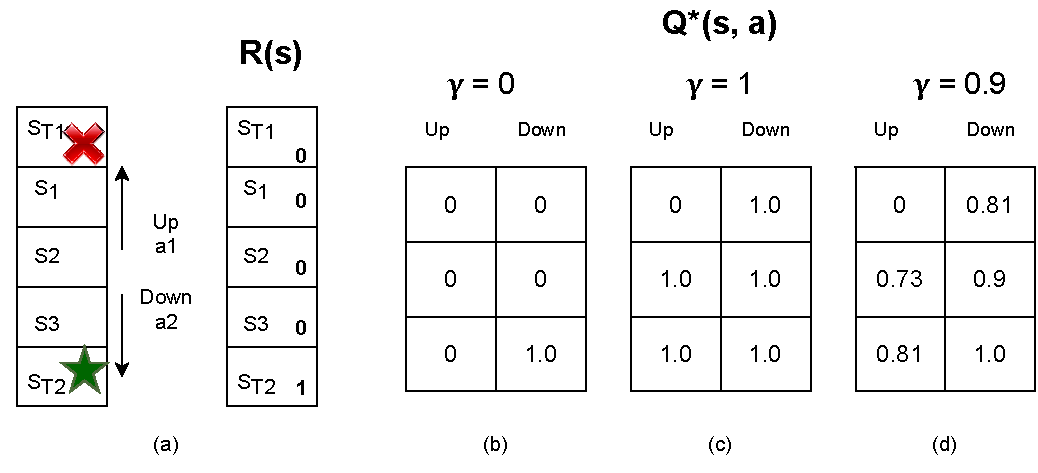
\includegraphics[height=2.5in]{figs/DRL-1d-Q_new}
\caption{
  Left: illustration of a simple MDP
  corresponding to a 1d grid world
  of 3 non-absorbing states and 2 actions.
  Right: optimal $Q$-functions for different values of $\gamma$.
\figbased{Figures 3.1, 3.2, 3.4 of \citep{Graesser2019}}.
}
\label{fig:Q1d}
\end{figure}

\section{Computing the value function and policy given a known world model}
\label{sec:planning}
\label{sec:rl-planning}
\label{sec:DPRL}

In this section, we discuss how
to compute the optimal value function (the \keywordDef{prediction problem})
and the optimal policy (the \keywordDef{control problem})
when the MDP model is known.
(Sometimes the term \keywordDef{planning} is used to refer
to computing the optimal policy, given a known model,
but planning can also refer to computing a sequence of actions,
rather than a policy.)
The algorithms we discuss are based on
\keywordDef{dynamic programming} (DP)
and \keywordDef{linear programming} (LP).

For simplicity, in this section, we assume
discrete state and action sets with $\gamma<1$.
However,
exact calculation of optimal policies often depends
polynomially on the sizes of $\calS$ and $\calA$,
and is intractable, for example, when the state space
is a Cartesian product of several finite sets.
This challenge is known as the
\keywordDef{curse of dimensionality}.
Therefore, approximations are typically needed,
such as using parametric or nonparametric representations of the value function or policy,
both for computational tractability and
for extending the methods to handle MDPs
with general state and action sets.
This requires the use of
\keywordDef{approximate dynamic programming} (ADP)
and \keywordDef{approximate linear programming} (ALP)
algorithms (see e.g., \cite{BertsekasRL}).

\eat{
using \keywordDef{dynamic programming} (\keywordDef{DP}).
The inputs to the algorithm
are the world model $p(s'|s,a)$
and reward function $R(s,a)$,
and the output is the optimal policy and 
its value function.
(This is called  \keywordDef{planning} using a known model.)
We assume the states and actions are discrete,
although similar methods can also be used in the linear-Gaussian case.
%(In fact the state space can be large, as long as $p(s'|s,a)$ is sparse.)
}

\subsection{Value iteration}
\label{sec:valueIter}
\label{sec:VI}

A popular and effective DP method for solving an MDP is
\keywordDef{value iteration} (VI).
Starting from an initial value function estimate $V_0$, the algorithm
iteratively updates the estimate by 
\begin{align}
\label{eqn:value-iteration}
V_{k+1}(s) = \max_a \left[
  R(s,a) + \gamma \sum_{s'} p(s'|s,a) V_k(s') \right]
\end{align}
Note that the update rule, sometimes called a
\keywordDef{Bellman backup},
is exactly the right-hand side of the Bellman optimality equation \cref{eqn:bellmanOptV}, with the unknown $\Vopt$ replaced by the current estimate $V_k$.
A fundamental property of \cref{eqn:value-iteration}
is that the update is a \keywordDef{contraction}:
it can be verified that
\begin{align}
\label{eqn:bellman-contraction}
\max_s |V_{k+1}(s) - \Vopt(s)| \le \gamma \max_s |V_k(s) - \Vopt(s)|
\end{align}
In other words, every iteration will reduce
the maximum value function error
by a constant factor.

$V_k$ will converge to $\Vopt$,
after which an optimal policy can be extracted using \cref{eqn:optPolFromV}.
In practice, we can often terminate VI
when $V_k$ is close enough to $\Vopt$,
since the resulting greedy policy wrt $V_k$
will be near optimal.
Value iteration can be adapted to learn the optimal action-value function $\Qopt$.

\subsection{Real-time dynamic programming (RTDP)}
\label{sec:RTDP}


In value iteration, we compute $\Vopt(s)$ and $\polopt(s)$
for all possible states $s$,
averaging over all possible next states $s'$ at each iteration,
as illustrated in \cref{fig:sutton-8-6}(right).
However, for some problems,
we may only be interested in the value (and policy)
for certain special starting states.
This is the case, for example, in
\keywordDef{shortest path problems} on graphs,
where we are trying to find the shortest
route from the current state to a goal state.
This can be modeled as an episodic MDP
by defining a transition matrix
$\ptran(s'|s,a)$ where
taking edge $a$ from node $s$ leads to the neighboring node $s'$
with probability 1.
The reward function is defined as $R(s,a)=-1$ for all states $s$
except the goal states,
which are modeled as absorbing
states.

In problems such as this, we can use a method
known as \keywordDef{real-time dynamic programming}
or \keywordDef{RTDP} \citep{Barto1995},
to efficiently compute an \keywordDef{optimal partial policy},
which only specifies what to do for the reachable states.
RTDP maintains a value function estimate $V$.
At each step, it performs a Bellman backup for the
current state $s$ by
$V(s) \assign \max_a \expectQ{R(s,a) + \gamma V(s')}{\ptran(s'|s,a)}$.
It picks an action $a$ (often with some exploration), reaches a next state $s'$,
and repeats the process.
%it picks an action $a$ for the current state $s$,
%according to $V$ (e.g., with an $\epsilon$-greedy exploration).
%It then performs a full
%expectation backup
%by computing $V(s) = \expectQ{R(s,a) + \gamma V(s')}{s'  \sim p(s'|s,a)}$.
%It then samples the next state $s'$,
%and repeats the process to update $V(s')$.
This can be seen as a form of the more general
\keywordDef{asynchronous value iteration},
that focuses its computational effort on parts of the state
space that are more likely to be reachable from the current state,
rather than synchronously updating all states at each iteration.
% Sutton p178

\subsection{Policy iteration}
\label{sec:policyIteration}

Another effective DP method for computing $\polopt$ is \keywordDef{policy iteration}.
It is an iterative algorithm that searches in the space
of deterministic policies until converging to an optimal policy.
Each iteration consists of two steps, \keywordDef{policy evaluation} and \keywordDef{policy improvement}.

The policy evaluation step, as mentioned earlier,
computes the value function for the current policy.
Let $\policy$ represent the current policy,
$\vv(s)=\Vpol(s)$ represent the value function encoded as a vector indexed by states,
$\vr(s) = \sum_a \policy(a|s) R(s,a)$ represent the reward vector,
and $\vT(s'|s) = \sum_a \policy(a|s) p(s'|s,a)$ 
represent the state transition matrix.
Bellman's equation for policy evaluation can be
written in the matrix-vector form as
\begin{align}
  \vv &= \vr + \gamma \vT \vv
  \label{eqn:policyEval}
  \end{align}
This is a linear system of equations in $|\cal{S}|$ unknowns.
We can solve it using matrix inversion:
$\vv = (\vI - \gamma \vT)^{-1} \vr$.
Alternatively, we can use value iteration
by computing
$\vv_{t+1} = \vr + \gamma \vT \vv_t$
until near convergence,
or some form of asynchronous variant
that is computationally more efficient.

Once we have evaluated $\Vpol$ for the current policy $\policy$,
we can use it to derive a better policy $\policy'$,
thus the name policy improvement.
To do this, we simply compute a deterministic
policy $\policy'$ that acts greedily with respect to $\Vpol$ in every
state, using
\be
\policy'(s) = \argmax_a \{R(s,a) + \gamma \expect{\Vpol(s')}\}
\ee
We can guarantee that $V_{\policy'} \ge \Vpol$.
This is called the \keywordDef{policy improvement theorem}.
To see this, define $\vr'$, $\vT'$ and $\vv'$ as before,
but for the new policy $\policy'$.
The definition of $\policy'$ implies
$\vr' + \gamma \vT' \vv \ge \vr + \gamma \vT \vv = \vv$,
where the equality is due to Bellman's equation.
Repeating the same equality, we have
\begin{align}
\vv &\le \vr' + \gamma \vT' \vv
\le \vr' + \gamma \vT' (\vr' + \gamma \vT' \vv)
\le \vr' + \gamma \vT' (\vr' + \gamma \vT' (\vr' + \gamma \vT' \vv) ) \le \cdots \\
&= (\vI + \gamma \vT' + \gamma^2 \vT'^2 + \cdots) \vr'
= (\vI - \gamma \vT')^{-1} \vr'
= \vv'
\end{align}

Starting from an initial policy $\policy_0$, policy iteration alternates
between policy evaluation ($E$)
and improvement ($I$) steps,
as illustrated below:
\begin{align}
\policy_0 \stackrel{E}{\ra} V_{\policy_0}
\stackrel{I}{\ra} \policy_1
\stackrel{E}{\ra} V_{\policy_1}
\cdots
\stackrel{I}{\ra} \polopt
\stackrel{E}{\ra} \Vopt
\end{align}
%where $E$ stands for policy evaluation and $I$ stands for policy improvement.
The algorithm stops at iteration $k$, if the policy $\policy_k$
is greedy with respect to its own value function $V_{\policy_k}$.
In this case, the policy is optimal.
Since there are at most $|\calA|^{|\calS|}$ deterministic policies,
and every iteration strictly improves the policy, the algorithm must converge after finite iterations.


%\label{sec:GPI}
In PI,
we alternate between policy evaluation (which involves multiple
iterations, until convergence of $\Vpol$),
and policy improvement.
In VI, we alternate between
one iteration of policy evaluation followed
by one iteration of policy improvement
(the ``$\max$'' operator in the update rule).
%In \keywordDef{generalized policy improvement} or \keywordDef{GPI},
We are in fact free to intermix any number of
these steps in any order.
The process will converge once the
policy is greedy wrt its own  value function.



\begin{figure}
\centering
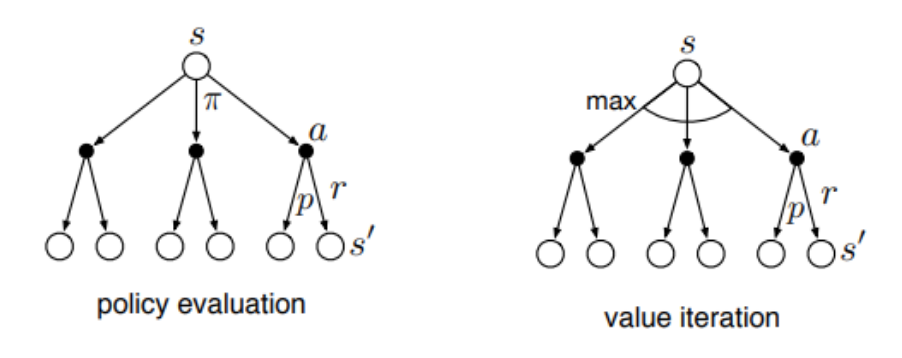
\includegraphics[height=1.5in]{figs/sutton-8-6-PI-VI}
\caption{
  Policy iteration vs value iteration represented as backup diagrams.
  Empty circles represent states, solid (filled) circles
  represent states and actions.
  \figbased{Figure 8.6 of \citep{Suttonv2}}.
}
\label{fig:sutton-8-6}
\end{figure}

Note that policy evaluation computes $\Vpol$
whereas value iteration computes $\Vopt$.
This difference is illustrated in \cref{fig:sutton-8-6},
using a \keywordDef{backup diagram}.
Here the root node represents any state $s$,
nodes at the next level represent state-action combinations
(solid circles),
and nodes at the leaves representing the set of possible
resulting next state $s'$ for each possible action.
In PE, we average over all actions according
to the policy, whereas in VI, we take the maximum over
all actions.

\section{Computing the value function  without knowing the world model}

In the rest of this chapter,
we assume the agent only has  access to samples from
the environment, $(s',r) \sim p(s',r|s,a)$.
We will show how to use these samples
to learn optimal value function and $Q$-function,
even without knowing the MDP dynamics.



\subsection{Monte Carlo estimation}
\label{sec:MCRL}

Recall that $\Vpol(s) = \expect{\return_t | s_t=s}$
is the sum of expected (discounted) returns from state $s$
if we follow policy $\pi$.
A simple way to estimate this is to rollout the policy,
and then compute the average
sum of discounted rewards.  The trajectory ends when we reach a terminal state, if
the task is episodic, or when the discount factor $\gamma^t$ becomes
negligibly small, whichever occurs first.
This is called \keywordDef{Monte Carlo estimation}.
We can use this to update our estimate of the value function as follows:
\begin{align}
\label{eqn:rl-td}
V(s_t) &\assign V(s_t) + \lr
\left[
 \return_t  - V(s_t)
  \right]
\end{align}
where $\lr$ is the learning rate, and the term in brackets is an error term.
We can use a similar technique to estimate
$\Qpol(s,a) = \expect{\return_t | s_t=s,a_t=a}$
by simply starting the rollout with action $a$.

We can use MC estimation of $Q$,  together with policy iteration
(\cref{sec:policyIteration}), to learn an optimal policy.
Specifically,
at iteration $k$,
we compute a new, improved policy using
$\policy_{k+1}(s) = \argmax_a Q_k(s,a)$,
where $Q_k$ is approximated using MC estimation.
This update can be applied to all the states visited
on the sampled trajectory.
This overall technique
is called \keywordDef{Monte Carlo control}.

To ensure this method converges to the optimal policy,
we need to collect data for every (state, action) pair,
at least in the tabular case,
since there is no generalization
across different values of $Q(s,a)$.
One way to achieve this is to use an $\epsilon$-greedy policy
 (see \cref{sec:epsGreedy}).
Since this is an on-policy algorithm,
the resulting method will converge
to the optimal $\epsilon$-soft policy,
as opposed to the optimal policy.
It is possible to use importance sampling
to estimate the value function for the optimal policy,
even if actions are chosen according to the $\epsilon$-greedy policy.
However, it is simpler to just gradually reduce $\epsilon$.
% Sutton p101

\subsection{Temporal difference (TD) learning}
\label{sec:TD}

The Monte Carlo (MC) method in \cref{sec:MCRL}
results in 
an estimator for $V(s)$ with very high variance,
since it has to unroll many trajectories, 
whose returns are a sum of many random rewards generated by stochastic state transitions.
%might yield very different returns.
In addition, it is limited to episodic tasks
(or finite horizon truncation of continuing tasks),
since it must unroll to the end of the episode
before each update step,
to ensure it reliably estimates the long term return.

In this section, we discuss a more efficient technique called
\keywordDef{temporal difference} or \keywordDef{TD} learning
\citep{Sutton88}.
The basic idea is to incrementally
reduce the Bellman error
%, which is the difference between the LHS and RHS of the Bellman equations,
for sampled states or state-actions,
based on transitions instead of a long trajectory.
More precisely, suppose we are to learn
the value function $\Vpol$ for a fixed policy $\policy$.
Given a state transition $(s_t,a_t,r_t,s_{t+1})$,
where $a_t \sim \policy(s_t)$,
we change the estimate $V(s_t)$ so that
it moves towards the  \keywordDef{target value}
$\targetV_t = r_t + \gamma V(s_{t+1}) \approx G_{t:t+1}$:
\begin{align}
V(s_t) &\assign V(s_t) + \lr
\left[
  \underbrace{r_t + \gamma V(s_{t+1}) - V(s_t)}_{\delta_t}
  \right]
%  &= (1-\lr) V(s_t) + \lr \big(r_t + \gamma V(s_{t+1}) \big) \notag
\end{align}
where $\lr$ is the learning rate.
(See \citep{Ryzhov2015} for ways to adaptively set the learning rate.)
The $\delta_t=y_t - V(s_t)$ term 
is known as the \keywordDef{TD error}.
A more general form of TD update
for parametric value function representations is
\begin{align}
\label{eqn:rl-td-approx}
\vw \assign \vw + \lr \left[
r_t + \gamma \Vapprox(s_{t+1})
  - \Vapprox(s_t) \right] \nabla_{\vw}\Vapprox(s_t)
\end{align}
we see that  \cref{eqn:rl-td} is a special case.
The TD update rule for evaluating $\Qpol$ is similar,
except we replace states with states and actions.

% Sutton and Bartoe p202

It can be shown that TD learning in the tabular case,
\cref{eqn:rl-td}, converges to the correct value function,
under proper conditions~\citep{BertsekasRL}.
%such as the the decay schedule of learning rate~\citep{BertsekasRL}.
However, it may diverge when using nonlinear function approximators,
as we discuss in \cref{sec:deadlytriad}.
The reason is that this update is a
``\keywordDef{semi-gradient}'',
which refers to the fact
that we only take the gradient wrt the  value function,
$\nabla_{\vw} V(\vs_t, \vw_t)$,
treating the target $U_t$ as constant.

The potential divergence of TD is also consistent with
the fact that \cref{eqn:rl-td-approx} does not correspond
to a gradient update
on any objective function, despite having
a very similar form to SGD (stochastic gradient descent).
Instead, it is an example of \keywordDef{bootstrapping},
%As mentioned in \cref{sec:rl-introl-valuebased},
%updates like \cref{eqn:rl-td} are based on
%the idea of \keywordDef{bootstrapping},
in which the estimate, $\Vapprox(s_t)$,
is updated to approach a target,
$r_t + \gamma \Vapprox(s_{t+1})$,
which is defined by the value function estimate itself.
This idea is shared by DP methods
like value iteration, although they rely on the
complete MDP model to compute an exact Bellman backup.
In contrast, TD learning can be viewed as using
sampled transitions to approximate such backups.
An example of a non-bootstrapping approach is the
Monte Carlo estimation in the previous section.
It samples a complete trajectory,
rather than individual transitions,
to perform an update;
this avoids the divergence issue,
but is  often much less
efficient.
\cref{fig:TD-MC-DP} illustrates the difference between
MC, TD, and DP.

\begin{figure}
\centering
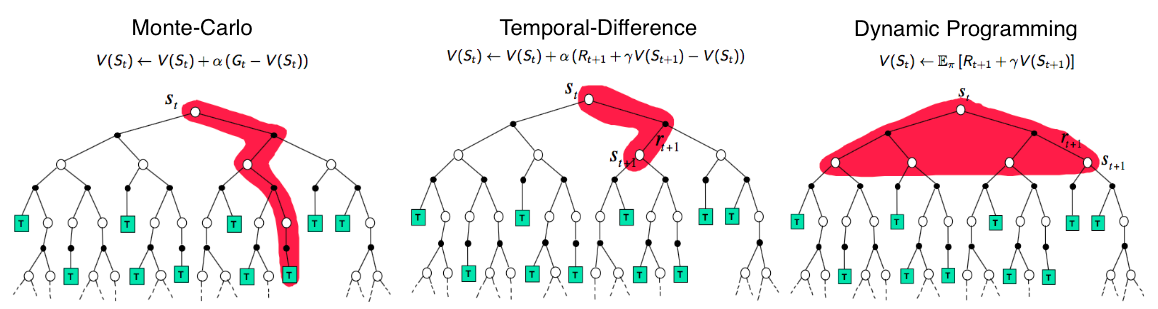
\includegraphics[height=1.5in]{figs/TD-MC-DP-backups}
\caption{
  Backup diagrams of $V(s_t)$ for Monte Carlo,
  temporal difference, and dynamic programming
  updates of the state-value function.
%  \figtaken{a figure from \citep{Silver2018L4}}.
%\figthanks{David Silver}.
\figthanks{Andy Barto}.
}
\label{fig:TD-MC-DP}
\end{figure}



\subsection{Combining TD and MC learning using TD($\lambda$)}
\label{sec:TDlambda}
\label{sec:nstep}

A key difference between TD and MC is
the way they estimate returns.
Given a trajectory
$\traj=(s_0,a_0,r_0,s_1,\ldots,s_T)$,
TD estimates the return from state $s_t$
by one-step lookahead,
$\return_{t:t+1} = r_t + \gamma V(s_{t+1})$,
where the return from time $t+1$ is replaced by
its value function estimate.
In contrast, MC waits until the end of the episode
or until $T$ is large enough,
then uses the estimate
$\return_{t:T} = r_t + \gamma r_{t+1} + \cdots + \gamma^{T-t-1} r_{T-1}$.
It is possible to interpolate between these by
performing an $n$-step rollout, and then using
the value function to approximate the return
for the rest of the trajectory,
similar to heuristic search (\cref{sec:heuristic}).
That is, we can use the \keywordDef{n-step return}
\begin{align}
\return_{t:t+n} = r_{t} + \gamma r_{t+1} + \cdots
+ \gamma^{n-1} r_{t+n-1} + \gamma^n V(s_{t+n})
\end{align}
For example, the 1-step and 2-step returns are given by
\begin{align}
  \return_{t:t+1} &= r_{t} + \gamma v_{t+1} \\
  \return_{t:t+1} &= r_{t} + \gamma r_{t+1} + \gamma^2 v_{t+2} \
  \end{align}
The corresponding $n$-step version of the TD update becomes
\begin{align}
  %V(s_t) \assign V(s_t) + \lr \left[\return_{t:t+n} - V(s_t)\right]
  \vw \assign \vw + \lr
  \left[\return_{t:t+n}  - \Vapprox(s_t) \right]
  \nabla_{\vw}\Vapprox(s_t)
\end{align}

Rather than picking a specific lookahead value, $n$,
we can take a weighted average of all possible values,
with a single parameter $\lambda\in[0,1]$,
by using
\begin{align}
\label{eqn:rl-gamma-return}
\return_{t}^{\lambda}
\defeq (1-\lambda) \sum_{n=1}^{\infty} \lambda^{n-1} \return_{t:t+n}
\end{align}
This is called the \keywordDef{lambda return}.
Note that these coefficients sum to one
(since $\sum_{t=0}^{\infty} (1-\lambda) \lambda^t = \frac{1-\lambda}{1-\lambda}=1$,
for $\lambda<1$),
so the return is a convex combination of $n$-step returns.
See \cref{fig:TDlambda} for an illustration.
We can now use $\return_t^{\lambda}$ inside the TD update
instead of $\return_{t:t+n}$;
this is called \keywordSpecial{TD$(\lambda)$}{TD(lambda)}.

Note that, if a terminal state is entered at step $T$ (as happens with episodic tasks),
then all subsequent $n$-step returns are equal to the conventional return, $G_t$.
Hence we can write
\begin{align}
  G_t^{\lambda} = (1-\lambda) \sum_{n=1}^{T-t-1}
  \lambda^{n-1} G_{t:t+n}
  \;
  + \lambda^{T-t-1} G_t
\end{align}
From this we can see that if $\lambda=1$, the $\lambda$-return
becomes equal to the regular MC return $G_t$.
If $\lambda=0$, the $\lambda$-return becomes equal to the
one-step return $G_{t:t+1}$ (since $0^{n-1}=1$ iff $n=1$),
so standard TD learning is often called
\keywordDef{TD(0) learning}.
This episodic form also gives us the following recursive equation
\be
G_t^{\lambda} = r_t + \gamma[(1-\lambda) v_{t+1} + \lambda G_{t+1}^{\lambda}]
\ee
which we initialize with $G_T=v_t$.
% https://github.com/google-deepmind/rlax/blob/master/rlax/_src/multistep.py#L34

\begin{figure}
\centering
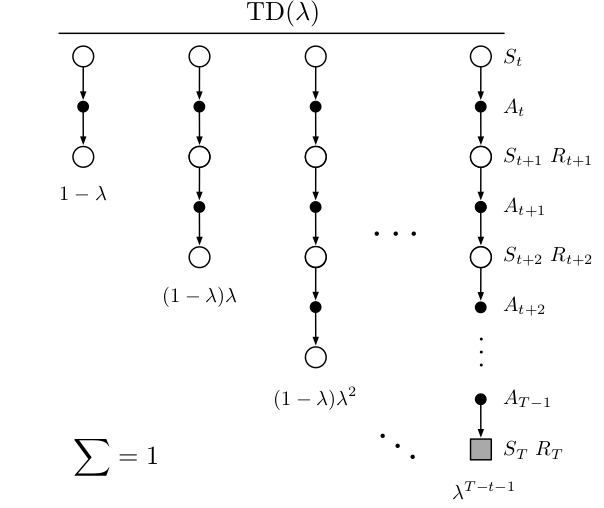
\includegraphics[height=2in]{figs/sutton-12-1}
\caption{
  The backup diagram for TD($\lambda$).
  Standard TD learning corresponds to $\lambda=0$,
  and standard MC learning corresponds to $\lambda=1$.
  \figtaken{Figure 12.1 of \citep{Suttonv2}}.
  \figthanks{Richard Sutton}.
}
\label{fig:TDlambda}
\end{figure}

\subsection{Eligibility traces}
\label{sec:eligibility}


An important benefit of using the geometric weighting
in \cref{eqn:rl-gamma-return}, as opposed to the $n$-step update,
is that
the corresponding TD learning update can be
efficiently implemented  through the use of
\keywordDef{eligibility traces},
even though $\return_{t}^{\lambda}$ is
a sum of infinitely many terms.
The eligibility term is a weighted sum of the gradients
of the value function:
\be
\vz_t = \gamma \lambda \vz_{t-1} + \nabla_{\vw} V_{\vw}(s_t)
\ee
(This trace term gets reset to 0 at the start of each episode.)
We replace the TD(0) update of
$\vw_{t+1} = \vw_t + \lr \delta_t \nabla_{\vw} V_{\vw}(s_t)$
with the TD($\lambda$) version to get
\be
\vw_{t+1} = \vw_t + \lr \delta_t \vz_t
\ee
See \citep{VanSeijen2016} for more details.

\section{SARSA: on-policy TD control}
\label{sec:SARSA}

TD learning is for policy evaluation,
as it estimates the value function for a fixed policy.
In order to find an optimal policy,
we may use the algorithm as a building block inside
generalized policy iteration (\cref{sec:policyIteration}).
In this case, it is more convenient
to work with the action-value function, $Q$, and
a policy $\policy$ that is greedy with respect to $Q$.
The agent follows $\policy$ in every step
to choose actions, and upon a transition $(s,a,r,s')$
the TD update rule is
\begin{align}
Q(s,a) \assign Q(s,a) + \lr \left[ r + \gamma Q(s',a') - Q(s,a) \right]
\label{eqn:rl-td-q}
\end{align}
where $a' \sim \policy(s')$ is the action
the agent will take in state $s'$.
After $Q$ is updated (for policy evaluation),
$\policy$ also changes accordingly as it is greedy
with respect to $Q$ (for policy improvement).
This algorithm, first proposed by \citep{Rummery1994},
was further studied and renamed to
\keywordDef{SARSA} by \citep{Sutton1996};
the name comes from its update rule that
involves an augmented transition $(s,a,r,s',a')$.

In order for SARSA to converge to $\Qopt$,
every state-action pair must be visited infinitely often,
at least in the tabular case,
since the algorithm only updates $Q(s,a)$
for $(s,a)$ that it visits.
One way to ensure this condition is to use a
``greedy in the limit with infinite exploration''
(\keywordDef{GLIE}) policy.
An example is the $\epsilon$-greedy policy,
with $\epsilon$ vanishing to $0$ gradually.
It can be shown that SARSA with a GLIE policy will
converge to $\Qopt$ and $\polopt$~\citep{Singh2000}.


\section{Q-learning: off-policy TD control}
\label{sec:Qlearning}

SARSA is an \keyword{on-policy} algorithm,
which means it learns the $Q$-function for the policy
it is currently using,
which is typically not the optimal policy,
because of the need to perform exploration.
However, with a simple modification,
we can convert this to an \keyword{off-policy}
algorithm that learns $\Qopt$,
even if a suboptimal or exploratory policy is used to choose actions.


\subsection{Tabular Q learning}

Suppose we modify SARSA by replacing the sampled next action
$a' \sim \policy(s')$ in \cref{eqn:rl-td-q}
with a greedy action:
$a' = \argmax_b Q(s',b)$.
This results in the following update
when a transition $(s,a,r,s')$ happens
\begin{align}
Q(s,a) \assign Q(s,a) + \lr \left[
  r + \gamma \max_{a'} Q(s',a') - Q(s,a) \right]
\label{eqn:Qlearning}
\end{align}
This is the update rule of \keywordDef{Q-learning}
for the tabular case~\citep{Watkins92}.


Since it is off-policy,
the method can use  $(s,a,r,s')$ triples
coming from any data source,
such as older versions of the policy,
or log data from an existing (non-RL) system.
If every state-action pair is visited infinitely often,
the algorithm provably converges to $\Qopt$
in the tabular case, with properly decayed learning rates~\citep{BertsekasRL}.
%See \cref{fig:oneStep} for a visual comparison of Q-learning,
%SARSA, TD and DP methods.
\cref{algo:Qlearning} gives a vanilla implementation of
Q-learning
%(with functiion approximation)
with $\epsilon$-greedy exploration.

\begin{algorithm}
\dontprintsemicolon
\caption{Tabular Q-learning with $\epsilon$-greedy exploration}
\label{algo:Qlearning}
Initialize value function $Q$ \\
\Repeat{converged}
       {
       Sample starting state $s$ of new episode \\
       \Repeat{state $s$ is  terminal}
       {
       Sample action
       $a=\begin{cases}
       \argmax_{b} Q(s,b), & \text{with probability $1-\epsilon$} \\
       \text{random action}, & \text{with probability $\epsilon$}
       \end{cases}$
               \\
       $(s',r) = \text{env.step}(a)$ \\
       Compute the TD error: $\delta = r + \gamma \max_{a'} Q(s',a') - Q(s,a)$ \\
       $Q(s,a) \leftarrow Q(s,a) + \lr \delta$ \\
       $s \leftarrow s'$ 
         }
}
\end{algorithm}

\eat{
\begin{algorithm}
\dontprintsemicolon
\caption{Q-learning with $\epsilon$-greedy exploration}
\label{algo:Qlearning}
Initialize value function parameters $\vw$ \\
\Repeat{converged}
       {
       Sample starting state $s$ of new episode \\
       \Repeat{state $s$ is  terminal}
       {
       Sample action
       $a=\begin{cases}
       \argmax_{b} \Qapprox(s,b), & \text{with probability $1-\epsilon$} \\
       \text{random action}, & \text{with probability $\epsilon$}
       \end{cases}$
               \\
       Observe state $s'$, reward $r$ \\
       Compute the TD error: $\delta = r + \gamma \max_{a'} \Qapprox(s',a') - \Qapprox(s,a)$ \\
       $\vw \assign \vw + \lr \delta \nabla_{\vw} \Qapprox(s,a)$ \\
           $s \assign s'$
         }
}
\end{algorithm}
}


%\subsection{Done states}
%\label{sec:done}

For terminal states, $s \in \calS^+$, we know that
$Q(s,a)=0$ for all actions $a$.
Consequently, for the optimal value function,
we have
$V^*(s) = \max_{a'} Q^*(s,a)=0$
for all terminal states.
%
When  performing online learning, we don't usually know
which states are terminal.
Therefore we assume that, whenever we take a step in the environment,
we get the next state $s'$ and reward $r$,
but also a binary indicator $\done(s')$ that tells us
if $s'$ is terminal.
In this case,  we set the target value in Q-learning
to $V^*(s')=0$ yielding the modified update rule:
\begin{align}
Q(s,a) \assign Q(s,a) + \lr \left[
  r + (1-\done(s')) \gamma \max_{a'} Q(s',a') - Q(s,a) \right]
\label{eqn:Qlearningdone}
\end{align}
For brevity, we will usually ignore this factor in the subsequent equations,
but it needs to be implemented in the code.

%\subsection{Example}
%\label{sec:Qlearning1d}


\begin{figure}
\centering
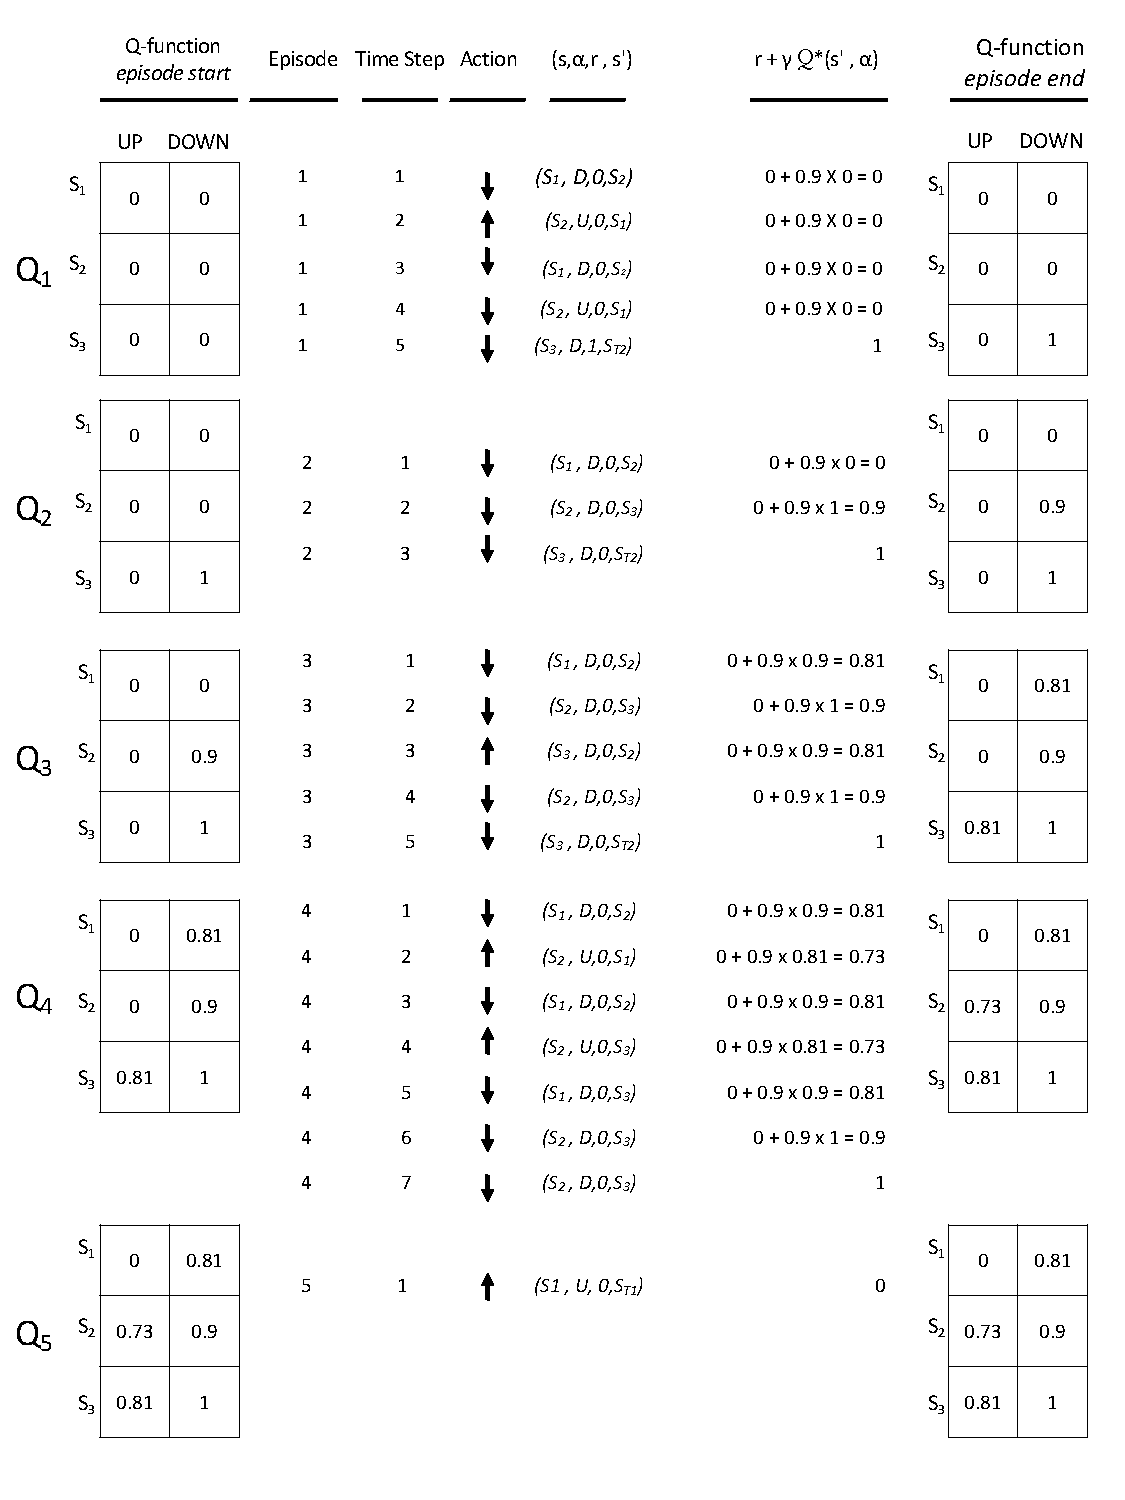
\includegraphics[height=5in]{figs/DRL-3-3}
\caption{
  Illustration of Q learning for one random trajectory
  in the 1d grid world
  in \cref{fig:Q1d} using $\epsilon$-greedy exploration.
  At the end of episode 1, we make a transition
  from $S_3$ to $S_{T2}$ and get a reward of $r=1$,
  so we estimate $Q(S_3,\downarrow)=1$.
  In episode 2, we make a transition from $S_2$ to $S_3$,
  so $S_2$ gets incremented by $\gamma Q(S_3,\downarrow)=0.9$.
  \figbased{Figure 3.3 of \citep{Graesser2019}}.
}
\label{fig:DRLTD}
\end{figure}

\cref{fig:DRLTD} gives an example
of Q-learning applied to the simple 1d grid world
from \cref{fig:Q1d}, using $\gamma=0.9$.
We show the $Q$-functon at the start and end of each episode,
after performing actions chosen by an $\epsilon$-greedy policy.
We initialize $Q(s,a)=0$ for all entries,
and use a step size of $\lr=1$.
At convergence, we have
$\Qopt(s,a) = r + \gamma \Qopt(s',a_*)$,
where $a_* = \downarrow$ for all states.




\subsection{Q learning with function approximation}
\label{sec:Qfn}

To make Q learning work with high-dimensional state spaces,
we have to replace the tabular (non-parametric) representation
with a parametric approximation, denoted $Q_{\vw}(s,a)$.
We can update this function using one or more steps of SGD
on the following loss function
\begin{align}
  \loss(\vw|\vs,a,r,\vs') &=
  \big( (r + \gamma \max_{a'} Q_{\vw}(\vs',a')) -   Q_{\vw}(\vs,a) \big)^2  
  \label{eqn:ynaive}
\end{align}
Since nonlinear functions need to be trained on minibatches
of data, we compute the average loss over multiple
randomly sampled
experience tuples (see \cref{sec:ER} for discussion)
  to get
  \begin{align}
\loss(\vw) &= \expectQ{\loss(\vw|\vs,a,r,\vs')}{(\vs,a,r,\vs') \sim U(\data)}
  \end{align}
%The random sampling helps reduce correlation between the samples.
%\begin{align}
%\vw  \assign \vw + \lr \left[
%  r + \gamma \max_{a'} Q_{_\vw}(s',a') - Q_{\vw}(s,a) \right]
%\nabla_{\vw} Q_{\vw}(s,a)
%\end{align}
See \cref{algo:Qfn} for the pseudocode.


\begin{algorithm}
\dontprintsemicolon
\caption{Q learning with function approximation and replay buffers}
\label{algo:Qfn}
Initialize environment state $\vs$,
network parameters $\vw_0$,
replay buffer $\data=\emptyset$,
discount factor $\gamma$,
step size $\eta$,
policy
$\pi_0(a|s) = \epsilon \text{Unif}(a)
+ (1-\epsilon) \delta(a=\argmax_a Q_{\vw_0}(s,a))$ \\
\For{iteration $k=0,1,2,\ldots$}
    {
      \For{environment step $s=0,1,\ldots,S-1$}
          {
            Sample action: $a \sim \pi_k(a|s)$ \\
            Interact with environment: $(s',r) = \text{env.step}(a)$ \\
            Update buffer: $\data \leftarrow \data \union \{ (s,a,s',r) \}$ 
          }
          $\vw_{k,0} \leftarrow \vw_k$ \\
          \For{gradient step $g=0,1,\ldots,G-1$}
              {
                Sample batch: $B \subset \data$ \\
                Compute error: $\loss(B,\vw_{k,g})
                = \frac{1}{|B|} \sum_{(s,a,r,s') \in B}
                \left[ Q_{\vw_{k,g}}(s,a) - (r + \gamma \max_{a'} Q_{\vw_k}(s',a')) \right]^2$\\
                Update parameters:
                $\vw_{k,g} \leftarrow \vw_{k,g} - \lr \nabla_{\vw_{k,g}}
                \loss(B,\vw_{k,g})$
              }
         $\vw_{k+1} \leftarrow \vw_{k,G}$ 
      }
\end{algorithm}

\subsubsection{Neural fitted Q}
\label{sec:NFQ}

The first approach of this kind
is known as \keywordDef{neural fitted Q iteration}
\citep{Riedmiller2005}, which corresponds to fully optimizing
$\loss(\vw)$ at each iteration (equivalent to using $G=\infty$
gradient steps).

\subsubsection{DQN}
\label{sec:DQN}

The influential
\keyword{deep Q-network} or \keyword{DQN}
paper of \citep{Mnih2015atari}
also used neural nets to represent the $Q$ function,
but performed a smaller number of gradient updates
per iteration.
Furthermore, they proposed to modify the target value
when fitting the $Q$ function in order to avoid
instabilities during training (see \cref{sec:deadly} for details).

The DQN method became famous since it was able  to train
agents that can outperform
humans when playing various Atari games from
the \keywordDef{ALE} (Atari Learning Environment)
benchmark \citep{Bellemare13}.
Here the input is a small color image,
and the action space corresponds to moving left, right, up or down,
plus an optional shoot action.\footnote{
%
For more discussion of ALE,
see \citep{Machado2018},
and for a recent extension to continuous actions
(representing joystick control),
see the CALE benchmark of \citep{Farebrother2024CALE}.
Note that DQN was not the first deep RL method to train
an agent from pixel input;
that honor goes to \citep{Lange2010},
who trained an autoencoder to embed images into low-dimensional latents,
and then used neural fitted Q learning (\cref{sec:NFQ})
to fit the $Q$ function.
}

Since 2015, many more extensions to DQN have been proposed,
with the goal of
improving performance in various ways,
either in terms of peak reward obtained,
or sample efficiency (e.g., reward obtained after only 100k steps
in the environment, as proposed in the \keywordDef{Atari-100k} benchmark
\citep{Atari100k}),
or training stability,
or all of the above.
We discuss some of these extensions in \cref{sec:DQNextensions}.



\eat{
\subsubsection{DQN}
\label{sec:DQN}


In this section, we discuss the seminal
\keywordDef{deep Q-network} or \keywordDef{DQN}
paper \citep{Mnih2015atari}.
The starting point is to consider the update
for the Q network parameters $\vw$
shown in \cref{algo:Qlearning}.
The gradient update corresponds to taking the gradient
of the following loss
\begin{align}
  \loss(\vw|\vs,a,r,\vs') &=
  \big( (r + \gamma \max_{a'} Q_{\vw}(\vs',a')) -   Q_{\vw}(\vs,a) \big)^2  
  \label{eqn:ynaive}
\end{align}
Since neural nets work best when trained on minibatches
of data, we compute the average loss by sampling
experience tuples (e.g., uniformly at random)
from
  the replay buffer $\data$
  (see \cref{sec:ER})
  to get
  \begin{align}
\loss(\vw) &= \expectQ{\loss(\vw|\vs,a,r,\vs')}{(\vs,a,r,\vs') \sim U(\data)}
  \end{align}
The random sampling helps reduce correlation between the samples.


\begin{algorithm}
\dontprintsemicolon
\caption{DQN (with target network)}
\label{algo:DQNtarget}
Initialize environment state $\vs$,
network parameters $\vw$,
target parameters $\overline{\vw} = \stopgrad(\vw)$,
replay buffer $\data=\emptyset$,
discount factor $\gamma$,
EMA rate $\rho$,
step size $\eta$
\\
\Repeat{converged}
       {
         Take action $a \sim \text{eps-greedy}(\vw)$\\
         $(\vs',r) = \text{step}(a, \vs)$ \\
         $\data := \data \union
         \{ (\vs, a, r, \vs') \}$ \\
         $\vs \assign \vs'$ \\
         Sample a minibatch $\calB = \{(\vs_j,a_j,r_j,\vs'_j)\}$
         from $\data$ \\
           $(\vw,\overline{\vw}) = \text{update}(\vw, \overline{\vw}, \calB)$
        }
.\\
$\text{def update}(\vw,\overline{\vw},\calB)$: \\
       Let $(\vs_j,a_j,r_j,\vs'_j)_{j=1}^B = \calB$ \\
$\targetV_{j} = \TargetV(r_j, \vs'_j; \overline{\vw})$ for $j=1:B$ \\
      $\loss(\vw) = \frac{1}{|\calB|} \sum_{(\vs_j, a_j, r_j, \vs'_j) \in
        \calB} (Q_{\vw}(\vs_j,a_j) - \stopgrad(\targetV_j))^2$\\
      $\vw \assign \vw - \lr_{\vw} \nabla \loss(\vw)$ // Gradient descent step \\
      $\overline{\vw} := \rho \overline{\vw} 
      + (1-\rho) \vw$       //EMA for  target network \\
    Return $\vw, \overline{\vw}$\\
\end{algorithm}
}


\subsubsection{Experience replay}
\label{sec:ER}
\label{sec:replay}

Since Q learning is an off-policy method, we can update the Q function
using any data source. This is particularly important when we use
nonlinear function approximation (see \cref{sec:Qfn}), which often needs a lot of data
for model fitting.
A natural source of data is data collected earlier in the trajectori
of the agent; this is called 
an \keywordDef{experience replay} buffer,
which stores  $(s,a,r,s')$ transition tuples into a buffer.
This can improve the stability and sample efficiency of learning,
and was
originally proposed in \citep{Lin1992}.

This modification has two advantages.
First, it improves data efficiency as every transition
can be used multiple times.
Second, it improves stability in training,
by reducing the correlation of the data samples
that the network is trained on,
since the training tuples do not have to come from
adjacent moments in time.
(Note that experience replay requires the use
of off-policy learning methods, such as Q learning,
since the training data is sampled from older
versions of the policy, not the current policy.)

%\subsubsection{Prioritized experience replay}
\label{sec:PER}

It is possible to replace the uniform sampling
from the buffer
with one that favors more
important transition tuples
that may be more informative about $Q$.
This idea is formalized in 
\citep{Schaul2016},
who develop a technique known as
\keywordDef{prioritized experience replay}.

\eat{
For example, we can sample transitions from $\data$
with probability
$p(s,a,r,s') \propto (|\delta| + \varepsilon)^{\eta}$,
%$p(i) = \frac{(|\delta_i| + \epsilon)^{\eta}}{(\sum_j |\delta_j|+\epsilon)^{\eta}}$,
where $\delta$ is the corresponding TD error
(under the current $Q$-function),
$\varepsilon > 0$ a hyperparameter
to ensure every experience is chosen
with nonzero probability,
and $\eta \geq 0$ controls the ``inverse temperature''
of the distribution (so $\eta=0$ corresponds to uniform sampling).
% Graesser p1110
}

\eat{
Consider the TD error for the $i$'th tuple $\tau_i$
\be
\delta_i = r_i + \gamma \max_{a'} Q_{\overline{\vw}}(s'_i, a')
 - Q_{\vw}(s_i,a_i)
\ee
Define the priority of $i$ as
\be
p_i = (\delta_i + \epsilon)^{\alpha}
\ee
where $\alpha \geq 0$ determines the degree of prioritization,
with $\alpha=0$ corresponding to no prioritization (uniform sampling).
Now define the probability of sampling $i$ as
\be
P(i) = \frac{p_i}{\sum_k p_k}
\ee
Sampling from this distribution will introduce bias relative
to the uniform distribution over the past $M$ samples in the replay buffer.
But we can correct this using importance sampling, as follows:
\begin{align}
  \expectQ{\loss(\tau)}{\text{Uniform}(\tau)}
  &= \sum_{i=1}^M \frac{1}{M} \loss(\tau_i) \\
  &= \sum_{i=1}^M P(\tau_i) \frac{1}{M P(\tau_i)} \loss(\tau_i) \\
  &= \expectQ{w(\tau) \loss(\tau)}{P(\tau)} 
  \end{align}
where we define the importance weight as
\be
w(\tau) = \left(\frac{1}{M P(\tau)} \right)^{\beta(t)}
\ee
Here $\beta(t)$ is a hyperparameter than starts off slightly larger than
0, to ensure that important experiences are not down-weighted too much,
and then is gradually increased to 1,
which results in an unbiased estimate.

%A distributed version of PER,
%known as \keywordDef{APE-X},
%is described in \citep{Horgan2018}.
}


\eat{
\subsubsection{Word of caution}

Unfortunately, when the function is nonlinear,
Q learning can become unstable; see \cref{sec:deadly} for details
of the problem and some solutions.
}






\subsubsection{The deadly triad}
\label{sec:offpolicyrl-deadlytriad}
\label{sec:deadlytriad}
\label{sec:deadlyTriad}
\label{sec:deadly}



\begin{figure}
\centering
\begin{subfigure}[b]{0.55\textwidth}
\centering
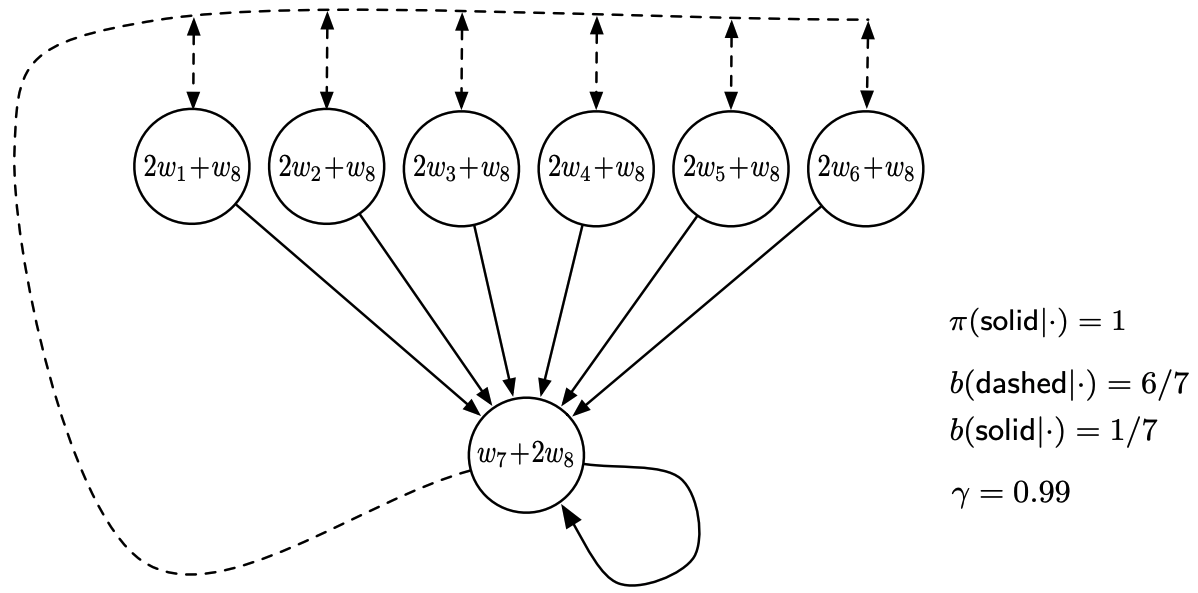
\includegraphics[height=1.75in]{figs/bairdExample}
\caption{ }
\label{fig:baird-example-mdp}
\end{subfigure}
~
\begin{subfigure}[b]{0.35\textwidth}
\centering
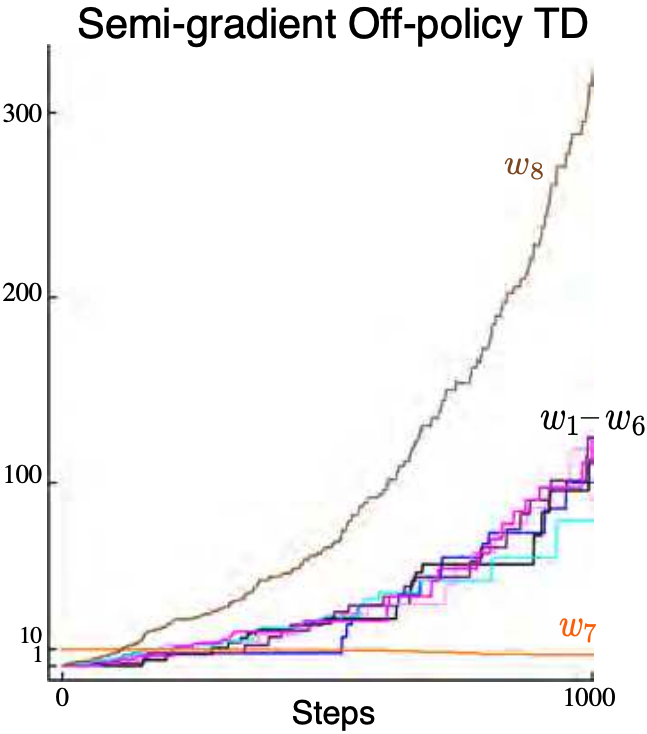
\includegraphics[height=1.75in]{figs/bairdExampleDivergence}
\caption{ }
\label{fig:baird-example-divergence}
\end{subfigure}
\caption{
(a) A simple MDP.
  (b) Parameters of the policy diverge over time.
\figtaken{Figures 11.1 and 11.2 of \citep{Suttonv2}}.
\figthanks{Richard Sutton}.
}
\label{fig:baird-example}
\end{figure}



The problem with the naive Q learning  objective in \cref{eqn:ynaive}
  is that it can lead to instability,
since the target we are regressing towards
uses the same parameters $\vw$ as the function we are updating.
So the network is ``chasing its own tail''.
Although this is fine for tabular models,  it can fail
for nonlinear models, as we discuss below.

In general, an RL algorithm can become unstable when it has
these three components:
function approximation (such as neural networks),
bootstrapped value function estimation (i.e., using TD-like methods instead of MC),
and off-policy learning (where the actions are sampled from some distribution
other than the policy that is being optimized).
This combination is known as \keywordDef{the deadly triad}
\citep{Sutton2015, Vanhasselt18}).
%It highlights another important challenge introduced by off-policy learning,
%and is a subject of ongoing research
%(e.g., \citep{Vanhasselt18,Kumar19}).

A classic example of this is the simple MDP depicted
in \cref{fig:baird-example-mdp}, due to \citep{Baird95}.
(This is known as \keywordDef{Baird's counter example}.)
It has 7 states and 2 actions.
Taking the dashed action takes the environment
to the 6 upper states uniformly at random,
while the solid action takes it to the bottom state.
The reward is 0 in all transitions,
and $\gamma=0.99$.
The value function $\Vapprox$ uses
a linear parameterization indicated by the expressions
shown inside the states, with $\vw\in\real^8$.
The target policies $\policy$ always chooses the
solid action in every state.
Clearly, the true value function, $\Vpol(s) = 0$,
can be exactly represented by setting $\vw=\vzero$.

Suppose we use a behavior policy $b$ to generate
a trajectory,
which chooses the dashed and solid actions
with probabilities $6/7$ and $1/7$, respectively,
in every state.
If we apply TD(0) on this trajectory,
the parameters diverge to $\infty$
(\cref{fig:baird-example-divergence}),
even though the problem appears simple.
In contrast, with on-policy data
(that is, when $b$ is the same as $\policy$),
TD(0) with linear approximation can be guaranteed to
converge to a good value function approximate~\citep{Tsitsiklis97}.
The difference is that with on-policy learning,
as we improve the value function, we also improve the policy,
so the two become self-consistent,
whereas with off-policy learning,
the behavior policy may not match the optimal
value function that is being learned,
leading to inconsistencies.


The divergence behavior is demonstrated in
many value-based bootstrapping methods, including TD, Q-learning,
and related approximate
dynamic programming algorithms,
where the value function is represented
either linearly (like the example above)
or nonlinearly~\citep{Gordon95,Tsitsiklis1997,Ostrovski2021}.
The root cause of these divergence phenomena
is that bootstrapping methods
typically are not minimizing a fixed objective function.  Rather, they
create a learning target using their own estimates, thus potentially
creating a self-reinforcing loop to push the estimates to infinity.
%In certain special cases, such a loop is not possible if data is
%on-policy, so one way to fix the problem is to apply off-policy
%correction methods discussed earlier.  
More formally, the problem is that
the contraction property in the tabular case
(\cref{eqn:bellman-contraction})
may no longer hold when $V$ is approximated by $\Vapprox$.

We discuss some solutions to the deadly triad problem below.


\subsubsection{Target networks}
\label{sec:targetNetwork}

One heuristic solution to the deadly triad,
proposed in the DQN paper,
is to use a  ``frozen'' 
\keywordDef{target network} computed at an earlier iteration
to define the target value for the DQN updates,
rather than trying to chase a constantly moving target.
Specifically, we maintain an extra copy
the $Q$-network, $Q_{\vw^-}$, 
with the same structure as $\Qapprox$.
This new $Q$-network is used
to compute bootstrapping targets
\be
\TargetV(r,\vs'; \vw^{-}) = r + \gamma \max_{a'} Q_{\vw^-}(\vs',a')
\ee
for training $\Qapprox$.
We can periodically set $\vw^{-} \assign \stopgrad(\vw)$,
usually after a few episodes,
where the stop gradient operator
is used to prevent autodiff propagating gradients back to $\vw$.
Alternatively, we can use
an exponential moving average (EMA)
of the weights,
i.e.,
we use 
 $\overline{\vw} = \rho \overline{\vw} + (1-\rho) \stopgrad(\vw)$,
where 
$\rho \ll 1$ ensures that $Q_{\overline{\vw}}$ slowly catches
up with $Q_{\vw}$.
(If $\rho=0$, we say that this is a \keywordDef{detached target},
since it is just a frozen copy of the current weights.)
The final loss  has the form
  \begin{align}
    \loss(\vw) &= \expectQ{\loss(\vw|\vs,a,r,\vs')}{(\vs,a,r,\vs') \sim U(\data)} \\
      \loss(\vw|\vs,a,r,\vs') &=
  (\TargetV(r,\vs';\overline{\vw}) -   Q_{\vw}(\vs,a))^2  
  \end{align}
%See \cref{algo:DQN} for the pseudocode.
Theoretical work justifying this technique is given
in  \citep{Fellows2023,Che2024}.


\eat{
\begin{algorithm}
\dontprintsemicolon
\caption{DQN (with target network)}
\label{algo:DQN}
Initialize environment state $\vs$,
network parameters $\vw$,
target parameters $\overline{\vw} = \stopgrad(\vw)$,
replay buffer $\data=\emptyset$,
discount factor $\gamma$,
EMA rate $\rho$,
step size $\eta$
\\
\Repeat{converged}
       {
         Take action $a \sim \text{eps-greedy}(\vw)$\\
         $(\vs',r) = \text{step}(a, \vs)$ \\
         $\data := \data \union
         \{ (\vs, a, r, \vs') \}$ \\
         $\vs \assign \vs'$ \\
         Sample a minibatch $\calB = \{(\vs_j,a_j,r_j,\vs'_j)\}$
         from $\data$ \\
           $(\vw,\overline{\vw}) = \text{update}(\vw, \overline{\vw}, \calB)$
        }
.\\
$\text{def update}(\vw,\overline{\vw},\calB)$: \\
       Let $(\vs_j,a_j,r_j,\vs'_j)_{j=1}^B = \calB$ \\
$\targetV_{j} = \TargetV(r_j, \vs'_j; \overline{\vw})$ for $j=1:B$ \\
      $\loss(\vw) = \frac{1}{|\calB|} \sum_{(\vs_j, a_j, r_j, \vs'_j) \in
        \calB} (Q_{\vw}(\vs_j,a_j) - \stopgrad(\targetV_j))^2$\\
      $\vw \assign \vw - \lr_{\vw} \nabla \loss(\vw)$ // Gradient descent step \\
      $\overline{\vw} := \rho \overline{\vw} 
      + (1-\rho) \vw$       //EMA for  target network \\
    Return $\vw, \overline{\vw}$\\
\end{algorithm}
}

\subsubsection{Two time-scale methods}

A general way to ensure convergence in off-policy
learning is to construct an objective function,
the minimization of which leads to a good value function approximation.
This is the basis of the
\keywordDef{gradient TD method} of \citep{Sutton2008,Maei2009,Ghiassian2020}.
%https://github.com/rlai-lab/Regularized-GradientTD
%see \citep[Ch.~11]{Suttonv2} for more information.
In practice, this can be achieved by  updating the target value in the TD update
more quickly than the value function itself;
this is known as a \keywordDef{two timescale optimization}
(see e.g., \citep{Yu2017TD,Zhang2019timescale,Hong2023}).
It is also possible to use a standard single timescale
method provided the target value is computed using a 
frozen \keyword{target network},
as discussed in \cref{sec:targetNetwork}.
See \citep{Fellows2023,Che2024} for details.

\subsubsection{Layer norm}

More recently, \citep{PQN} proved that just adding LayerNorm
\citep{Ba2016}
to the penultimate layer of the critic network,
just before the linear head,
is sufficient  to provably yield convergence of TD learning
even in the off-policy setting.
In particular, suppose the network has the form
$Q(s,a|\vw,\vtheta) = \vw^T \relu(\text{LayerNorm}(f(s,a;\vtheta)))$.
Since $||\text{LayerNorm}(f(s,a;\vtheta))|| \leq 1$, we have
$||Q(s,a|\vw,\vtheta) \leq ||\vw||$,
which means the magnitude of the output is always bounded,
as shown in \cref{fig:layerNorm}.
In \citep{PQN}, they prove this (plus $\ell_2$ regularization on $\vw$,
and a sufficiently wide penultimate layer)
is sufficient to ensure convergence 
of the value function estimate.



\begin{figure}
\centering
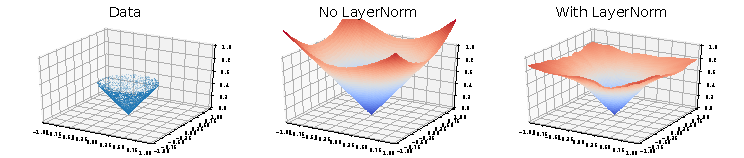
\includegraphics[height=1.5in]{figs/LayerNormFigure}
\caption{
  We generate a dataset (left) with inputs $\vx$
  distributed in a circle with radius 0.5 and labels $y = ||\vx||$.
  We then fit a two-layer MLP without LayerNorm (center)
  and with LayerNorm (right).
  LayerNorm bounds the values and prevents catastrophic overestimation
  when extrapolating.
  \figtaken{Figure  3 of \citep{Ball2023}}.
  \figthanks{Philip Ball}.
}
\label{fig:layerNorm}
\end{figure}



\eat{
% Bo Dai

  Thanks for asking! First, the deadly triad is offpolicy data + general function + TD. We can break the deadly triad by either use optimization based method to replace TD (e.g., LP-based RL with primal-dual solver https://arxiv.org/pdf/2001.01866), or use overparametrized general function (https://arxiv.org/abs/2405.21043). Second, linear value function with appropriate basis is also powerful. We had a series of work on developing the appropriate linear basis (representation) for RL (https://arxiv.org/pdf/2208.09515). Third, for convex Q function, I do not have general answer for general dynamics. However, for the multi-stage stochastic optimization  dynamic problem (https://arxiv.org/pdf/2112.00874), the Q is proved to be convex and TD converges.

 % Tom Zahavy.
  We had this paper on convex RL: https://openreview.net/pdf?id=ELndVeVA-TR, in this case we focus on value functions that are convex in the occupancy (while the value function is linear in it). These functions are quite popular for exploration/diversity/imitation so this convex setting is actually rich and meaningful. The problems are almost equivalent in terms of hardness results.

%  Hado van Hasselt.
  TD with linear value functions also suffers from the deadly triad in the off-policy case, though gradient TD (GTD) algorithms exist that do converge (in addition to alternatives Bo Dai mentioned above).

  Non-linear TD can additionally diverge even in the *on-policy* case. See, e.g., this classic paper by John Tsitsiklis and  @Benjamin Van Roy.
[Tsitsiklis1997]
  I conjecture that convexity in the parameters will not be sufficient to avoid this divergence.  If useful, I could try to construct a simple example to demonstrate this.  (I haven't checked carefully, maybe the example in the paper above is already convex.)

  However, for some problems even non-linear TD is guaranteed to converge.  For instance, this paper by Yann Ollivier
[Ollivier2018]
  that shows non-linear TD converges when the MDP is reversible, because then TD can be interpreted as stochastic gradient descent on a different objective (and therefore then inherits standard convergence properties of SGD).

Strict divergence does not always seem to happen, btw, when using a different optimiser, like ADAM, because this bounds the parameter updates.  This doesn't solve the issue, because the values can still get increasingly inaccurate when using an unstable update (we've called this phenomenon 'soft divergence' in the past).
}



\subsection{Maximization bias}

\begin{figure}
\centering
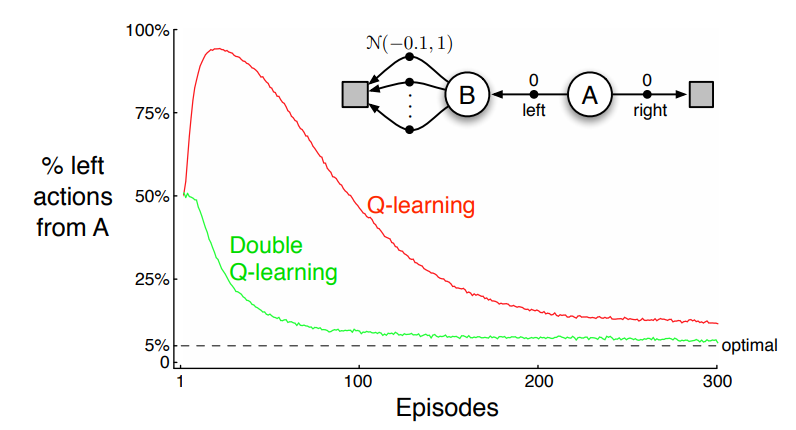
\includegraphics[height=1.5in]{figs/sutton-6-5}
\caption{
  Comparison of Q-learning and double Q-learning on a simple episodic
  MDP using $\epsilon$-greedy action selection with $\epsilon=0.1$.
  The initial state is A, and squares denote absorbing states.
The data are averaged over 10,000 runs.
\figtaken{Figure 6.5 of \citep{Suttonv2}}.
\figthanks{Richard Sutton}.
}
\label{fig:sutton-6-5}
\end{figure}

Standard Q-learning suffers from a problem
known as the \keywordDef{optimizer's curse} \citep{Smith2006},
or the \keywordDef{maximization bias}.
The problem refers to the simple statistical inequality:
$\expect{\max_a X_a} \geq \max_a \expect{X_a}$,
for a set of random variables $\{X_a\}$.
%where $r_i \sim p(R)$ are samples of $R$.
Thus, if we pick actions greedily according to their random scores $\{X_a\}$, we might pick a wrong action just because random noise makes it appealing.

% p135
\cref{fig:sutton-6-5} gives a simple example
of how this can happen in an MDP.
The start state is A.
The right action gives a reward 0 and terminates the episode.
The left action also gives a reward of 0,
but then enters state B,
from which there are many possible actions,
with rewards drawn from $\gauss(-0.1, 1.0)$.
Thus the expected return for any trajectory starting with the left
action is $-0.1$, making it suboptimal.
Nevertheless, the RL algorithm may pick   the left action
due to the maximization bias making B appear to have a positive value.

\subsubsection{Double Q-learning}
\label{sec:double}

One solution to avoid the maximization bias is to
use two separate $Q$-functions, $Q_1$ and $Q_2$,
one for selecting the greedy action,
and the other for estimating the corresponding $Q$-value.
%$\argmax_a Q_1(s,a)$,
%and the other of which is used to estimate the value
%of the chosen action, $Q_2(s,a_*)$.
%This estimate is unbiased,
%since $\expect{Q_2(s,a_*)}=Q(s,a_*)$.
%At each step, we perform the following update
In particular, upon seeing a transition $(s,a,r,s')$,
we perform the following update for $i=1:2$:
\begin{align}
  Q_i(s,a) &\assign Q_i(s,a) + \lr(\targetV_i(s,a) - Q_i(s,a)) \\
  \targetV_i(s,a) &= r + \gamma Q_{i}(s', \argmax_{a'} Q_{-i}(s', a'))
  \label{eqn:doubleQ}
%Q_1(s,a) \assign Q_1(s,a) + \lr \left[
%  r + \gamma Q_2\big(s', \argmax_{a'} Q_1(s',a')\big) -
%  Q_1(s,a) \right]
\end{align}
%% In particular, the training target for $Q_1$ becomes
%% $y_t =  r_{t+1} + \gamma Q_2(s_{t+1}, \argmax_a Q_1(s_{t+1},a))$.
%% (Alternatively, we can use
%% $y_t =  r_{t+1} + \gamma Q_1(s_{t+1}, \argmax_a Q_2(s_{t+1},a))$
%% as a training target for $Q_1$'
%% the choice is made randomly.)
So we see that $Q_1$ uses $Q_2$ to choose the best action
but uses $Q_1$ to evaluate it,
and vice versa.
%and may repeat the same update but with the roles
%of $Q_1$ and $Q_2$ swapped.
%We can also swap the roles of $Q_1$ and $Q_2$.
This technique is called
\keywordDef{double Q-learning} \citep{vanHasselt2010}.
\cref{fig:sutton-6-5} shows the benefits of
the algorithm over standard Q-learning
in a toy problem.

\subsubsection{Double DQN}
\label{sec:doubleDQN}


In \citep{vanHasselt2016}, they combine double Q learning
with deep Q networks (\cref{sec:DQN}) to get \keywordDef{double DQN}.
This modifies \cref{eqn:doubleQ}
to its gradient form, and then the current network for action
proposals, but the target network for action evaluation.
Thus  the  training target becomes
\be
\TargetV(r,\vs'; \vw, \overline{\vw}) = r + \gamma
Q_{\overline{\vw}}(\vs', \argmax_{a'} Q_{\vw}(\vs',a'))
\ee

In \cref{sec:TD3} we discuss an extension called
\keywordDef{clipped double DQN} which uses two Q networks
and their frozen copies
to define
the following target:
\be
\TargetV(r,\vs'; \vw_{1:2}, \overline{\vw}_{1:2}) = r + \gamma  \min_{i=1,2}
Q_{\overline{\vw}_i}(\vs',\argmax_{a'} Q_{\vw_i}(\vs',a'))
\ee
where $Q_{\overline{\vw}_i}$ is the target network for $Q_{\vw_i}$.
%We can derive a policy from the two networks by taking their average
%\be
%\pi(\vs,\vw) = \argmax_a \frac{1}{2} \sum_{i=1}^2 Q(\vs,a;\vw_i)
%\ee

\subsubsection{Randomized ensemble DQN}
\label{sec:REDQ}

The double DQN method is extended in
the \keywordDef{REDQ} (randomized ensembled double Q learning)
method of \citep{REDQ},
which uses
an ensemble of  $N>2$ Q-networks.
Furthermore, at each step, it draws a random
sample of $M \leq N$ networks, and takes the minimum over them
when computing the target value.
That is, it uses the following update
(see Algorithm 2 in appendix of \citep{REDQ}):
\be
\TargetV(r,\vs'; \vw_{1:N}, \overline{\vw}_{1:N})
= r + \gamma \max_{a'} \min_{i \in \calM} Q_{\overline{\vw}_i}(\vs',a')
\label{eqn:REDQtabular}
\ee
where $\calM$ is a random subset from the $N$ value functions.
The ensemble reduces the variance, and the minimum reduces
the overestimation bias.\footnote{
%
In addition, 
REDQ performs $G \gg 1$  updates of the value functions
for each environment step;
this  high \keywordDef{Update-To-Data} (UTD) ratio
(also called \keywordDef{Replay Ratio})
is critical for sample efficiency,
and is commonly used in model-based RL.
}
If we set $N=M=2$, we get a method
similar to clipped double Q learning.
(Note that REDQ is very similiar to the
\keywordDef{Random Ensemble Mixture} method of
\citep{Agarwal2020}, which was designed for offline RL.)



\eat{

See \cref{algo:REDQ} for some pseudocode for REDQ
for the tabular case.

\begin{algorithm}
\dontprintsemicolon
\caption{Tabular REDQ with experience replay}
\label{algo:REDQ}
Initialize $\{Q_i(s,a)\}_{i=1}^N$, $\overline{Q}_i=Q_i$ \\
$\hat{Q}(s,a) = \frac{1}{N} \sum_{i=1}^N Q_i(s,a)$\\
Initialize state $s$ \\
\Repeat{converged}
       {
         $a=\text{eps-greedy}(\hat{Q}(s,\cdot))$ \\
         $(s',r) = \text{step}(a,s)$\\
         $\data := \data \union \{ (s,a,r,s') \}$ \\
         \For{$G$ updates}
             {
               Sample a tuple $(s,a,r,s')$  from $\data$ \\
               Sample a set of $M$ indices $\calM \subseteq \{1,\ldots,N\}$ \\
               $Q_{\calM}(s,a) \defeq \min_{i \in \calM} \overline{Q}_i(s,a)$  \\
               Compute the  target 
               $\targetV(s,a) = r + \gamma \max_{a'} Q_{\calM}(s',a')$  \\
             \For{$i=1:N$}
                 {
                   $Q_i(s,a) \assign Q_i(s,a) + \lr(\targetV(s,a)-Q_i(s,a))$
                 }
             }
             $\hat{Q}(s,a) = \frac{1}{N} \sum_{i=1}^N Q_i(s,a)$\\
          $s \assign s'$
}
\end{algorithm}

}



\subsection{DQN extensions}
\label{sec:DQNextensions}

In this section, we discuss various extensions of DQN.

\subsubsection{Q learning for continuous actions}
\label{sec:QTopt}

Q learning is not directly applicable to continuous actions due to the need
to compute the argmax over actions.
An early solution to this problem,
based on neural fitted Q learning (see \cref{sec:NFQ}),
is proposed in \citep{Hafner2011}.
This became the basis of the 
DDPG algorithm of \cref{sec:DDPG},
which learns a policy to predict
the argmax.

An alternative  approach is to use gradient-free optimizers such as
the cross-entropy method to approximate the argmax.
The \keywordDef{QT-Opt} method of \citep{QTopt}
treats  the action vector $\va$ as a sequence of actions,
and optimizes one dimension at a time \citep{Metz2017}.
The  \keywordDef{CAQL} (continuous action $Q$-learning) method
of \citep{CAQL})
uses mixed integer programming to solve the $\argmax$ problem,
leveraging the \relu structure  of the $Q$-network.
The method of \citep{Seyde2022} quantizes each action dimension separately,
and then solves the argmax problem using methods inspired by  multi-agent RL.

  

\subsubsection{Dueling DQN}
\label{sec:duelingDQN}

The  \keywordDef{dueling DQN} method of \citep{Wang2016dueling},
learns a value function and an advantage function,
and derives the Q function, rather than learning it directly.
  This is helpful  when there are many actions with similar
$Q$-values, since the advantage $A(s,a)=Q(s,a)-V(s)$ focuses
  on the differences in value relative to a shared baseline.

In more detail, we define a network with $|A|+1$ output heads,
which computes  $A_{\vw}(\vs,a)$ for $a=1:A$ and
$V_{\vw}(\vs)$. We can then derive
\be
Q_{\vw}(\vs,a) = V_{\vw}(\vs) + A_{\vw}(\vs,a)
\ee
However, this naive approach ignores the following constraint
that holds for any policy $\pi$:
\begin{align}
\expectQ{A^{\pi}(s,a)}{\pi(a|s)}
&= \expectQ{Q^{\pi}(s,a) - V^{\pi}(s)}{\pi(a|s)} \\
&= V^{\pi}(s)  - V^{\pi}(s) = 0
\end{align}
Fortunately, for the optimal policy
$\pi^*(s) = \argmax_{a'} Q^*(s,a')$ we have
\begin{align}
0 
&= \expectQ{Q^*(s,a)}{\pi^*(a|s)}  - V^*(s) \\
&= Q^*(s, \argmax_{a'} Q^*(s,a')) - V^*(s) \\
&= \max_{a'} Q^*(s,a') - V^*(s) \\
&= \max_{a'} A^*(s,a')
\end{align}
Thus we can satisfy the constraint for the optimal policy
by subtracting off   $\max_a A(s,a)$ from the advantage head.
Equivalently we can compute the Q function using 
\be
Q_{\vw}(\vs,a) = V_{\vw}(\vs) + A_{\vw}(\vs,a) - \max_{a'} A_{\vw}(\vs,a')
\ee
In practice, the max is replaced by an average,
which seems to work better empirically.

\subsubsection{Noisy nets and exploration}
\label{sec:noisyDQN}
\label{sec:noisyNets}

Standard DQN relies on the epsilon-greedy strategy to perform exploration.
However, this will explore equally in all states,
whereas we would like to the amount of exploration
to be state dependent, to reflect the amount of uncertainty
in the outcomes of trying each action in that state
due to lack of knowledge (i.e., \keywordDef{epistemic uncertainty}
rather than aleatoric or irreducile uncertainty).
An early approach to this,
known as  \keywordDef{noisy nets} \citep{Fortunato2018},
added random noise to
the network weights to encourage exploration which is
temporally consistent within episodes.
More recent methods for exploration
are discussed in \cref{sec:exploreExploit}.
%are discussed in \cref{sec:intrinsicReward}.


\subsubsection{Multi-step DQN}
\label{sec:nsteps}

As we discussed in \cref{sec:TDlambda},
we can reduce the bias introduced by bootstrapping
by replacing TD(1) updates with TD($n$) updates,
where we unroll the value computation for $n$ MC steps,
and then plug in the value function at the end.
We can apply this to the DQN context by defining the target
\be
\targetV(s_0,a_0) = \sum_{t=1}^n \gamma^{t-1} r_t
 + \gamma^n \max_{a_n} Q_{\vw}(s_n, a_n)
 \ee
This can be implemented for episodic environments
by storing experience tuples of the form
\be
\tau = (s, a, \sum_{k=1}^n \gamma^{k-1} r_k, s_n, \done)
\ee
where $\done=1$ if the trajectory ended at any point
during the $n$-step rollout.
 
Theoretically this method is only valid if all the intermediate
actions, $a_{2:n-1}$, are sampled from the current optimal policy
derived from $Q_{\vw}$,
as opposed to some behavior policy,
such as epsilon greedy or some samples from the replay buffer
from an old policy.
In practice, we can just restrict sampling
to  recent samples from the replay buffer,
making the resulting method approximately on-policy.

Instead of using a fixed $n$, it is possible
to use a weighted combination of returns;
this is known as the  $Q(\lambda)$
  algorithm \citep{Peng1994,Kozuno2021}.

    

\eat{
\subsection{Putting it all together}

Many of the above methods can be combined for improved performance.
We give some examples of such hybrid methods below.
(Note that, besides combining various algorithmic pieces,
careful hyper-parameter tuning is critical for good results,
as discussed in \citep{Obando-Ceron2024}.)
}

\subsubsection{Rainbow}
\label{sec:rainbow}

The \keywordDef{Rainbow} method of \citep{rainbow}
combined 6 improvements to the vanilla DQN method,
as listed below.
(The paper is called ``Rainbow'' due to the color coding
of their results plot, a modified version of which is shown in
\cref{fig:rainbow}.)
At the time it was published (2018), this produced 
SOTA results on the Atari-200M benchmark.
The 6 improvements are as follows:
\begin{itemize}
\item Use \keyword{double DQN}, as in \cref{sec:doubleDQN}.

    \item  Use 
  \keyword{prioritized experience replay},  as in \cref{sec:PER}.

  
\item  Use the
categorical DQN (C51) (\cref{sec:C51}) 
distributional RL method.

  \item Use n-step returns (with $n=3$), as in \cref{sec:nsteps}.
  
\item Use \keyword{dueling DQN}, as in \cref{sec:duelingDQN}.

\item Use \keyword{noisy nets}, as in \cref{sec:noisyNets}.
\end{itemize}
Each improvement gives diminishing returns,
as can be see in \cref{fig:rainbow}.

\begin{figure}
\centering
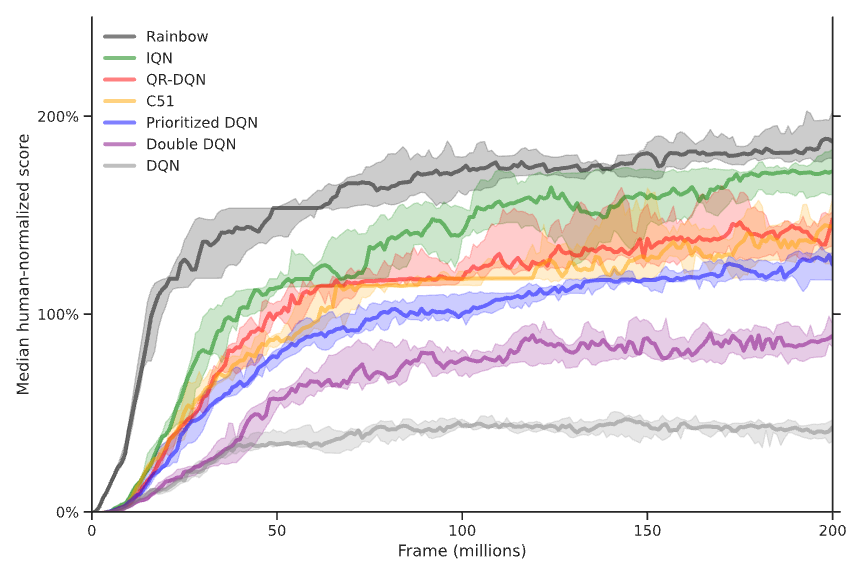
\includegraphics[height=1.5in]{figs/rainbow}
\caption{
  Plot of median human-normalized score over all 57 Atari games for
  various DQN agents.
  The yellow, red and green curves are distributional RL methods
  (\cref{sec:distributional}),
  namely categorical DQN (C51) (\cref{sec:C51})
  Quantile Regression DQN (\cref{sec:QRDQN}),
  and Implicit Quantile Networks \citep{IQN}.
  Figure from \url{https://github.com/google-deepmind/dqn_zoo}.
}
\label{fig:rainbow}
\end{figure}



Recently the ``Beyond the Rainbow'' paper \citep{beyond} proposed
several more extensions: 
\begin{itemize}
\item Use a larger CNN with residual connections,
  namely the Impala
  network from \citep{Espeholt2018}
  with the modifications (including the use of spectral normalization)
  proposed in
  \citep{Schmidt2021atari}.

  \item  Replace C51 with Implicit Quantile Networks \citep{IQN}.

  \item Use \keywordDef{Munchausen RL} \citep{Vieillard2020},
    which modifies
    the Q learning update rule by adding an entropy-like
    penalty.

  \item Collect 1 environment step from 64 parallel workers
    for each minibatch update (rather than taking many steps
    from a smaller number of workers).
\end{itemize}


\eat{
    \footnote{
    %
    The idea is as follows.
    First note that Q learning defines a greedy policy
    $\pi(a|s)=1$ iff $a = \argmax_{a'} Q(s,a')$,
    which we can convert to a stochastic policy
    $\pi(a|s) = \frac{\exp Q(s,a)}{\sum_{a'} Q(s,a')}$.
    Now consider the experience tuple
    $(s,a,r,s')$, so the Q learning
    target becomes $\targetV(s,a) = r + \max_{a'} Q^*(s',a')$.
Since $Q^*$ is unknown, we replace it with the current estimate
$Q_{\vw}(s',a')$ to get $\targetV(s,a) = r+q$ where $q=\max_{a'} Q_{\vw}(s',a')$.
However, this bootstrapping process can be unstable.
To help improve it, we can replace the target $r +q$ with
$r + \alpha \log \pi(a|s) + q$;
the motivation for this regularizer is that
the optimal policy should satisfy $\log \pi^*(a|s)$.
}
}


\subsubsection{Bigger, Better, Faster}
\label{sec:BBF}



At the time of writing this document (2024),
the SOTA on the 100k sample-efficient
Atari benchmark
\citep{Atari100k}
is obtained by the \keywordDef{BBF} algorithm of \citep{BBF}.
(BBF stands for ``Bigger, Better, Faster''.)
%This is arguably simpler than Rainbow.
It uses the following tricks,
in order of decreasing importance:
\begin{itemize}



\item Use a larger CNN with residual connections,
  namely a modified version of the Impala
  network from \citep{Espeholt2018}.

  \item Increase the \keywordDef{update-to-data} (UTD)
  ratio
  (number of times we update the Q function
  for every observation that is observed), in order to increase
  sample efficiency
  \citep{VanHasselt2019}.


\item Use a periodic soft reset of (some of) the network weights
to avoid loss of elasticity due to increased network updates, following the
\keywordDef{SR-SPR} method of \citep{DOro2022}.


\item Use n-step returns, as in \cref{sec:nsteps},
  and then gradually decrease (anneal) the n-step return from
 $n=10$ to $n=3$,
to reduce the bias over time.


\item Add weight decay.

\item Add a \keyword{self-predictive representation} loss
  (\cref{sec:self-predictive})
 to increase sample efficiency.

\item  Gradually increase the discount factor from
  $\gamma=0.97$ to $\gamma=0.997$,
  to encourage longer term planning once the model starts to be trained.\footnote{
  %
    The \keywordDef{Agent 57} method of  \citep{Badia2020}
  automatically learns the exploration rate and discount factor
  using a multi-armed bandit stratey,
  which lets it  be more exploratory or more exploitative,
  depending on the game. This resulted in super human performance
  on all 57 Atari games in ALE.
  However, it required 80 billion frames (environment steps)!
  This was subsequently reduced to the ``standard''
  200M frames in the \keywordDef{MEME} method of \citep{Kapturowski2022}.
  }


\item Drop noisy nets (which requires multiple network copies and thus slows
  down training due to increased memory use), since it does not help.

\item Use
  \keyword{dueling DQN} (see \cref{sec:duelingDQN}).

\item Use
  \keyword{distributional DQN}
  (see \cref{sec:distributional}).
  
%\item Use RNN models for the Q network,
%  as proposed in  the \keywordDef{R2D2} paper \citep{R2D2},
%  and used in many other papers.

\end{itemize}

\subsubsection{Other methods}

Many other methods have been proposed to reduce the sample complexity
of value-based RL while maintaining performance,
see e.g., the \keywordDef{MEME} paper of
\citep{Kapturowski2022}.






%\chapter{Policy-based RL}
\label{sec:policySearch}



%https://lilianweng.github.io/lil-losg/2018/04/08/policy-gradient-algorithms.html

In the previous section, we considered methods that
estimate the action-value function, $Q(s,a)$,
from which we derive a policy.
%If $Q$ is close to $\Qopt$,
%the resulting policy will be near optimal.
%e.g., $\policy(a|s)=\ind{a=\argmax_a Q(s,a)}$
%or $\policy(a|s) = e^{Q(s,a)}/\sum_{a'} e^{Q(s,a')}$.
However, these methods have several disadvantages:
(1)  they can be difficult to apply to continuous action spaces;
(2) they may diverge if function approximation is used (see
\cref{sec:deadlyTriad});  
(3) the training of $Q$, often based on TD-style updates,
is not directly related to the expected return
garnered by the learned policy;
(4) they learn deterministic policies,
whereas in stochastic and partially observed environments,
stochastic policies are provably better
\citep{Jaakkola94}.

In this section, we discuss
\keywordDef{policy search} methods,
which directly optimize the parameters of the policy
so as to maximize its expected return.
We mostly focus on \keywordDef{policy gradient} methods,
that use the gradient of the loss to guide the search.
As we will see,  these policy methods often 
benefit from estimating a value or advantage function
to reduce the variance in the policy search process,
so we will also use techniques from \cref{sec:valueRL}.
The parametric policy will be denoted by 
$\pi_{\vtheta}(a|s)$.
For discrete actions, this can be a DNN with a softmax output.
For continuous actions, we can use a Gaussian output layer,
or a diffusion policy \citep{Ren2024}.

For more details on policy gradient methods, see \citep{weng2018PG,Lehmann2024}.



\eat{
\footnote{
%
To handle multimodal distributions, it has recently
become popular to use more expressive policy classes such as diffusion
models;
this is known as a \keywordDef{diffusion policy}
\citep{diffusionPolicy}.
However, since it is difficult to compute the probability
value of the output from diffusion, such models are usually
trained using behavior cloning (\cref{sec:BC}),
rather than the policy gradient methods we discuss in this section.
%(For a recent survey of other ways to apply diffusion in RL,
%see \citep{diffusionRL}.)
}
}

\section{The policy gradient theorem}
\label{sec:policyGradient}
\label{sec:PG}


%http://timvieira.github.io/blog/post/2019/04/20/the-likelihood-ratio-gradient/

We start by defining the objective function
for policy learning,
and then derive its gradient.
%We consider the episodic case.
%A similar result can be derived for the continuing case with the average reward
%criterion~\citep[Sec 13.6]{Suttonv2}.
The objective, which we aim to maximize, is defined as
\begin{align}
  J(\pi)  &\defeq \expectQ{\sum_{t=0}^{\infty} \gamma^t R_{t+1}}{\pi} \\
  &= \sum_{t=0}^{\infty} \gamma^t \sum_s \left(\sum_{s_0}
  p_0(s_0) p^{\pi}(s_0 \rightarrow s, t) \right)
  \sum_a \pi(a|s) R(s,a) \\
  &= \sum_s 
  \left(
  \sum_{s_0} \sum_{t=0}^{\infty} \gamma^t 
  p_0(s_0) p^{\pi}(s_0 \rightarrow s, t) \right)
  \sum_a \pi(a|s) R(s,a) \\
  &= \sum_s \rho^{\pi}(s)    \sum_a \pi(a|s) R(s,a) 
\end{align}
where we have defined the discounted state visitation
measure
\be
\statmeasure_{\pi}^{\gamma}(s) \defeq
\sum_{t=0}^{\infty} \gamma^t
\underbrace{\sum_{s_0}   p_0(s_0) p^{\pi}(s_0 \rightarrow s, t)}_{p_t^{\pi}(s)}
\ee
where
$p^{\pi}(s_0 \ra s, t)$ is the probability of going
from $s_0$ to $s$ in $t$ steps,
and
$p_t^{\pi}(s)$ is the marginal probability of being in state $s$
at time $t$ (after each episodic reset).
Note that $\statmeasure_{\pi}^{\gamma}$ is a measure of time spent in  non-terminal states,
but it is not a probability measure, since it is not normalized,
i.e., $\sum_s \statmeasure_{\pi}^{\gamma}(s) \neq 1$.
However, we may abuse notation and still treat it like a probability,
so we can write things like
\be
\expectQ{f(s)}{\statmeasure_{\pi}^{\gamma}(s)} =
\sum_s \statmeasure_{\pi}^{\gamma}(s) f(s)
\ee
Using this notation, we can define the objective as
\be
J(\pi) = \expectQ{R(s,a)}{\statmeasure_{\pi}^{\gamma}(s), \pi(a|s)}
\label{eqn:JJpi}
\ee
We can also define a normalized version of the measure $\statmeasure$
by noting that
$\sum_{t=0}^{\infty} \gamma^t = \frac{1}{1-\gamma}$ for $\gamma<1$.
Hence the normalized discounted state visitation distribution
is given by
\be
\statdistpol(s) = (1-\gamma) \statmeasure_{\pi}^{\gamma}(s)
= (1-\gamma) \sum_{t=0}^{\infty} \gamma^t p_t(s)
\label{eqn:statdistpol}
\ee
(Note the change from $\rho$ to $p$.)

Note that in 
\citep[Sec 13.2]{Suttonv2}, they use slightly different notation.
In particular, they assume $\gamma=1$,
and define the non-discounted state visitation measure
as $\eta(s)$ and the corresponding normalized version by $\mu(s)$.
This is equivalent to ignoring  the discount factor $\gamma^t$
when defining $\statmeasure_{\pi}(s)$.
This is standard practice in many implementations,
since we can just average over (unweighted)
trajectories when estimating
the objective and its gradient,
even though it
results in a biased estimate
\citep{Nota2020,Che2023}.

It can be shown that the gradient of the above objective is
given by
\begin{align}
\nabla_{\vtheta} J(\vtheta)
&=\sum_s \statmeasure_{\pi}^{\gamma}(s)
\sum_a Q^{\pi}(s,a) \nabla_{\vtheta} \pi_{\vtheta}(a|s)
\label{eqn:PGthm}
\\
&=\sum_s \statmeasure_{\pi}^{\gamma}(s)
\sum_a Q^{\pi_{\vtheta}}(s,a) \pi_{\vtheta}(a|s) \nabla_{\vtheta} \log \pi_{\vtheta}(a|s) \\
&=\expectQ
{Q^{\pi_{\vtheta}}(s,a) \nabla_{\vtheta} \log \pi_{\vtheta}(a|s)}
    {\statmeasure_{\pi}^{\gamma}(s) \pi_{\vtheta}(a|s)} 
\label{eqn:SFE}
\end{align}
This is known as the \keywordDef{policy gradient theorem}
\citep{Sutton99b}.
In statistics, the term $\nabla_{\vtheta} \log \pi_{\vtheta}(\va|\vs)$
is called the (Fisher) \keywordDef{score function}\footnote{
%
This is distinct from the Stein score,
which is the gradient wrt the argument of the log probability,
$\nabla_{\va} \log \pi_{\vtheta}(\va|\vs)$,
as used in diffusion.
},
so sometimes \cref{eqn:SFE}
is called the \keywordDef{score function estimator}
or \keywordDef{SFE} \citep{Fu2015,Mohamed2020}.



\section{REINFORCE}
\label{sec:REINFORCE}
\label{sec:reinforceOpt}
\label{sec:reinforce}

% Pieter Abeel lecture notes
%https://drive.google.com/file/d/0BxXI_RttTZAhY216RTMtanBpUnc/view


% Sutton p327
One way to apply the policy gradient theorem
to optimize a policy is to use stochastic gradient ascent.
Theoretical results concerning the convergence
and sample complexity of such
methods can be found in \citep{Agarwal2021}.

To implement such a method,
let
$\traj=(s_0,a_0,r_0,s_1,\ldots,s_T)$ be
a trajectory created by sampling from $s_0\sim\initdist$
and then following $\polapprox$.
Then we have
\begin{align}
\nabla_{\vtheta} \polval(\polapprox)
&=
\sum_{t=0}^{\infty} \gamma^t \expectQ{
  \nabla_{\vtheta} \log \polapprox(a_t|s_t) \Qpolapprox(s_t,a_t)}
    {p_t(s) \polapprox(a_t|s_t)} \\
  &\approx \sum_{t=0}^{T-1} \gamma^t \return_t \nabla_{\vtheta} \log\polapprox(a_t|s_t)
\end{align}
where the return  is defined as follows
\begin{align}
\return_t &\defeq r_t + \gamma r_{t+1} + \gamma^2 r_{t+2} + \cdots
+ \gamma^{T-t-1} r_{T-1} 
= \sum_{k=0}^{T-t-1} \gamma^k r_{t+k}
= \sum_{j=t}^{T-1} \gamma^{j-t} r_j
\end{align}
See \cref{algo:REINFORCE} for the pseudocode.

\begin{algorithm}
\dontprintsemicolon
\caption{REINFORCE (episodic version)}
\label{algo:REINFORCE}
Initialize policy parameters $\vtheta$\\
\Repeat{converged}
       {
         Sample an episode $\traj=(s_0, a_0, r_0, s_1, \ldots, s_T)$ using $\polapprox$ \\
         %Compute $\return_t$ for all $t\in\{0,1,\ldots,T-1\}$ using \cref{eqn:rl-return} \\
         \For{$t=0,1,\ldots,T-1$}{
           $\return_t = \sum_{k=t+1}^T \gamma^{k-t-1} R_k$ \\
           $\vtheta \assign \vtheta + \lr_{\vtheta} \gamma^t \return_t
           \nabla_{\vtheta} \log \policy_{\vtheta}(a_t|s_t)$
         }
}
\end{algorithm}

In practice, estimating the policy gradient using
\cref{eqn:SFE} can have a high variance.
A \keywordDef{baseline} function $b(s)$ can be used for variance reduction
to get
\begin{align}
\nabla_{\vtheta} \polval(\polapprox) = 
 \expectQ{\nabla_{\vtheta} \log \polapprox(a|s) (\Qpolapprox(s,a) - b(s))}
{\statmeasure_{\vtheta}(s) \polapprox(a|s)}
\label{eqn:PGthmBaseline}
\end{align}
Any function that satisfies $\expect{\nabla_{\vtheta} b(s)}=0$ is a valid
baseline.
This follows since
\be
\sum_a  \nabla_{\vtheta} \pi_{\vtheta}(a|s) (Q(s,a)-b(s))
= \nabla_{\vtheta} \sum_a \pi_{\vtheta}(a|s) Q(s,a)
-\nabla_{\vtheta} [\sum_a \pi_{\vtheta}(a|s)] b(s)
= \nabla_{\vtheta} \sum_a \pi_{\vtheta}(a|s) Q(s,a) - 0
\ee
A common choice for the baseline is $b(s) = \Vpolapprox(s)$.
This is a good choice since $\Vpolapprox(s)$ and $Q(s,a)$ are correlated
and have similar magnitudes,
so the scaling factor in front of the gradient term will be small.
%(See also \citep{Wu2018} for an action-dependent baseline.)

Using this we get an update of the following form
\begin{align}
  \vtheta \assign \vtheta + \lr \sum_{t=0}^{T-1}
  \gamma^t (G_t - b(s_t)) \nabla_{\vtheta} \log\polapprox(a_t|s_t)
\label{eqn:REINFORCE}
\end{align}
This is 
is called the \keywordDef{REINFORCE} estimator
\citep{Williams1992}.\footnote{
  %
  The term 
``REINFORCE'' is an acronym for
``REward Increment = nonnegative Factor x Offset
Reinforcement x Characteristic Eligibility''.
The phrase ``characteristic eligibility'' refers to  the
$\nabla \log \polapprox(a_t|s_t)$ term;
the phrase ``offset reinforcement'' refers to the
$\return_t-b(s_t)$ term;
and the phrase ``nonnegative factor''
refers to the learning rate $\lr$ of SGD.
} %
The update equation
 can be interpreted as follows:
we compute the sum of discounted future rewards
induced by a trajectory, compared to a
baseline,  and if this is positive, we increase
$\vtheta$ so as to make this trajectory more likely,
otherwise we decrease $\vtheta$.
Thus, we reinforce good behaviors,
and reduce the chances of generating bad ones.



\eat{
\cref{algo:REINFORCEbaseline} gives the pseudocode
where we use  separate learning rates
for the two objectives.

\begin{algorithm}
\dontprintsemicolon
\caption{REINFORCE (episodic) with value function baseline}
\label{algo:REINFORCEbaseline}
Initialize policy parameters $\vtheta$, baseline parameters $\vw$\\
\Repeat{converged}
       {
         Sample an episode $\traj=(s_0, a_0, r_0, s_1, \ldots, s_T)$ using $\polapprox$ \\
         %Compute $\return_t$ for all $t\in\{0,1,\ldots,T-1\}$ using \cref{eqn:rl-return} \\
         \For{$t=0,1,\ldots,T-1$}{
           $\return_t = \sum_{k=t+1}^T \gamma^{k-t-1} R_k$ \\
           $\delta_t = \return_t - \Vapprox(s_t)$  \\
           $\vw \assign \vw - \lr_{\vw} \delta_t \nabla_{\vw}
           \Vapprox(s_t)$  \\
           $\vtheta \assign \vtheta + \lr_{\vtheta} \gamma^t \delta_t
           \nabla_{\vtheta} \log \policy_{\vtheta}(a_t|s_t)$ 
         }
}
\end{algorithm}
}


\section{Actor-critic methods}
\label{sec:actorCritic}
\label{sec:AC}



An \keywordDef{actor-critic} method \citep{Barto1983}
uses the policy gradient method,
but where the expected return $G_t$ is estimated
using temporal difference learning
of a value function instead of MC rollouts.
(The term ``actor'' refers to the policy,
and the term ``critic'' refers to the value function.)
The use of bootstrapping in TD updates
allows more efficient learning of the value function
compared to MC, and further reduces the variance.
In addition, it allows us to develop a fully online, incremental
algorithm, that does not need to wait until the end of the trajectory
before updating the parameters.


\subsection{Advantage actor critic (A2C)}
\label{sec:A2C}
\label{sec:A3C}

% Sutton p331
Concretely, consider the use of the one-step TD method
to estimate the return in the episodic case,
i.e., we replace $\return_t$ with
$\return_{t:t+1}=r_t+ \gamma \Vapprox(s_{t+1})$.
If we use $\Vapprox(s_t)$ as a baseline,
the REINFORCE update in \cref{eqn:REINFORCE} becomes
\begin{align}
\vtheta 
&\assign \vtheta + \lr \sum_{t=0}^{T-1} \gamma^t \left(G_{t:t+1} - \Vapprox(s_t)\right) \nabla_{\vtheta} \log\polapprox(a_t|s_t) \\
&= \vtheta + \lr \sum_{t=0}^{T-1} \gamma^t \big(r_t+ \gamma \Vapprox(s_{t+1}) - \Vapprox(s_t)\big) \nabla_{\vtheta} \log\polapprox(a_t|s_t)
\end{align}

%This  can be extended to the off-policy
%setting as explained in e.g., \citep{Degris2012,Zhang2019}.
%https://medium.com/@jonathan_hui/rl-policy-gradients-explained-advanced-topic-20c2b81a9a8b



Note that
$\delta_t = r_{t+1} + \gamma \Vapprox(s_{t+1}) -\Vapprox(s_t)$
is a single sample approximation
to the advantage function $A(s_t,a_t) = Q(s_t,a_t) - V(s_t)$.
%We can alternatively learn the advantage function
%directly, and use $A(s_t,a_t)$ instead
%of $\return_{t:T}$ (as in vanilla REINFORCE),
%or $\return_t^{(1)}$ (as in REINFORCE with a TD(0) baseline).
This method is therefore called 
\keywordDef{advantage actor critic} or \keywordDef{A2C}.
See \cref{algo:A2C} for the pseudo-code.\footnote{
%
In \citep{A3C}, they proposed
a distributed version of A2C known as
\keywordDef{A3C} 
which stands for  ``asynchrononous advantage actor critic''. 
}
(Note that $V_{\vw}(s_{t+1})=0$ if $s_t$ is a done state,
representing the end of an episode.)
Note that this is an on-policy algorithm,
where we update the value function $V_{\vw}^{\pi}$
to reflect the value of the current policy $\pi$.
See \cref{sec:bilevel} for further discussion of this point.

% https://github.com/DLR-RM/stable-baselines3/blob/master/stable_baselines3/a2c/a2c.py


\begin{algorithm}
\dontprintsemicolon
\caption{Advantage actor critic (A2C) algorithm (episodic)}
\label{algo:A2C}
Initialize actor parameters $\vtheta$, critic parameters $\vw$\\
\Repeat{converged}
       {
       Sample starting state $s_0$ of a new episode \\
       \For{$t=0,1,2,\ldots$}
       {
         Sample action $a_t \sim \polapprox(\cdot|s_t)$ \\
         $(s_{t+1},r_t,\done_t) = \text{env.step}(s_t,a_t)$ \\
        $\targetV_t = r_t + \gamma (1-\done_t) \Vapprox(s_{t+1})$       // Target \\
       $\delta_t = \targetV_t - \Vapprox(s_t)$ // Advantage \\
           $\vw \assign \vw  + \lr_{\vw} \delta_t \nabla_{\vw}
       \Vapprox(s_t)$ // Critic \\
           $\vtheta \assign \vtheta + \lr_{\vtheta} \gamma^t \delta_t
       \nabla_{\vtheta} \log \polapprox(a_t|s_t)$ // Actor \\
       \If{$\done_t=1$}{break}
         }
}
\end{algorithm}

In practice, we should use a stop-gradient
operator on the target value for the TD update,
for reasons  explained in \cref{sec:deadlyTriad}.
Furthermore, it is common to add an entropy term
to the policy, to act as a regularizer
(to ensure the policy remains stochastic, which smoothens
the loss function --- see \cref{sec:SAC}).
If we use a shared network with separate value  and policy heads,
we need to use a single loss function for training all the parameters
$\vphi$.
Thus we get the following loss, for each trajectory,
where we want to minimize TD loss,
maximize the policy gradient (expected reward) term,
and maximize the entropy term.
\begin{align}
  \loss(\vphi;\tau) &= \frac{1}{T} \sum_{t=1}^T \left[
    \lambda_{TD} \loss_{TD}(s_t,a_t,r_t,s_{t+1})
    -    \lambda_{PG} J_{PG}(s_t,a_t,r_t,s_{t+1})
    -    \lambda_{ent} J_{ent}(s_t)
    \right]
  \label{eqn:ACloss}\\
  \targetV_t &= r_t + \gamma (1-\done(s_t)) V_{\vphi}(s_{t+1}) \\
  \loss_{TD}(s_t,a_t,r_t,s_{t+1})  &= (\stopgrad(\targetV_t) - V_{\phi}(s))^2 \\
  J_{PG}(s_t,a_t,r_t,s_{t+1}) &= (\stopgrad(\targetV_t - V_{\phi}(s_t))
  \log \pi_{\vphi}(a_t|s_t) \\
  J_{ent}(s_t) &= -\sum_a \pi_{\vphi}(a|s_t) \log \pi_{\vphi}(a|s_t)
\end{align}
To handle the dynamically varying scales of the different loss functions,
we can use 
the \keywordDef{PopArt} method
of \citep{van-Hasselt2016,Hessel2019}
to allow for a fixed set of hyper-parameter values for $\lambda_i$.
(PopArt  stands for
``Preserving Outputs Precisely, while Adaptively Rescaling Targets''.)

\eat{
\begin{align}
  \loss(\vphi;\tau) = \frac{1}{T} \sum{t=1}^T \left[
    \lambda_{TD} (\stopgrad(\targetV_t) - V_{\vphi}(\vs_t))^2
    -    \lambda_{PG} (\stopgrad(\targetV_t - V_{\vphi}(\vs_t))
    -    \lambda_{ent} \entropy(\pi_{\vphi}(\cdot|\vs_t))
    \right]
  \end{align}
}

\eat{
We can then accumulate  the following gradients
over each sampled trajectory:
\begin{align}
  \nabla_{\vw}  &= -\frac{1}{2T} \sum_t
  \nabla_{\vw} (\targetV_t - V_{\vw}(s_t))^2 
  = \frac{1}{T} \sum_t  (\targetV_t - V_{\vw}(s_t)) \nabla_{\vw} V_{\vw}(s_t) \\
  \nabla_{\vtheta} &= \frac{1}{T} \sum_t
  (\targetV_t - V_{\vw}(s_t)) \nabla_{\vtheta} \log \pi_{\vtheta}(a_t|s_t)
  \end{align}
The second gradient ignores the discount term $\gamma^t$,
but omitting this is standard practice,
even though it
results in a biased estimate
\citep{Nota2020,Che2023}.
}


\eat{
For a more practical minibatch version,
based on \citep{Ivanov2019},
see \cref{algo:A2C}.
}

\subsection{Generalized advantage estimation (GAE)}
\label{sec:GAE}

%\subsection{AC with $n$-step critics}

In A2C, we replaced the high variance, but unbiased,
MC return $G_t$
with the low variance, but biased,
one-step bootstrap return $G_{t:t+1} = r_t + \gamma V_{\vw}(s_{t+1})$.
More generally, we can compute the
$n$-step estimate
\begin{align}
G_{t:t+n} =
r_t + \gamma r_{t+1} + \gamma^2 r_{t+2}
+ \cdots + \gamma^{n-1} r_{t+n-1} + \gamma^n \Vapprox(s_{t+n})
\end{align}
and thus obtain  the (truncated) $n$-step advantage estimate as follows:
\be
A_{\vw}^{(n)}(s_t,a_t) = G_{t:t+n} - \Vapprox(s_t)
\ee
Unrolling to infinity, we get
% https://nn.labml.ai/rl/ppo/gae.html
\begin{align}
  A_t^{(1)} &= r_t + \gamma v_{t+1} - v_t  \\
  A_t^{(2)} &= r_t + \gamma r_{t+1} + \gamma^2 v_{t+2} - v_t  \\
  &\vdots \\
  A_t^{(\infty)} &= r_t + \gamma r_{t+1} + \gamma^2 r_{t+2} +\cdots - v_t 
  \end{align}
$A_t^{(1)}$ is high bias but low variance,
and $A_t^{(\infty)}$  is unbiased but high variance.


%https://nn.labml.ai/rl/ppo/gae.html
% https://github.com/google-deepmind/rlax/blob/master/rlax/_src/multistep.py#L39
% https://github.com/EdanToledo/Stoix/blob/main/stoix/utils/multistep.py#L12
% https://github.com/luchris429/purejaxrl/blob/main/purejaxrl/ppo.py#L142
%https://github.com/DLR-RM/stable-baselines3/blob/master/stable_baselines3/common/buffers.py#L402

Instead of using a single value of $n$, we can take
a weighted average.
That is, we define
\be
A_t = \frac{\sum_{n=1}^T w_n A_t^{(n)}}{\sum_{n=1}^T w_n}
\ee
If we set $w_n = \lambda^{n-1}$ we get the following simple recursive
calculation:
\begin{align}
  \delta_t &= r_t + \gamma v_{t+1} - v_t \\
  A_t &= \delta_t + \gamma \lambda \delta_{t+1} + \cdots +
  (\gamma \lambda)^{T-t+1} \delta_{T-1} = \delta_t + \gamma \lambda
  A_{t+1}
  \end{align}
Here $\lambda \in [0,1]$ is a parameter that controls the bias-variance
tradeoff: larger values decrease the bias but increase the variance.
This is called \keywordDef{generalized advantage estimation}
(\keywordDef{GAE})~\citep{GAE}.
See \cref{algo:GAE} for some pseudocode.
Using this, we can define a general actor-critic
method, as shown in \cref{algo:AC}.

\begin{algorithm}
\dontprintsemicolon
\caption{Generalized Advantage Estimation}
\label{algo:GAE}
$\text{def GAE}(r_{1:T},v_{1:T}, \gamma, \lambda)$\\
$A'=0$ \\
\For{$t=T:1$}{
  $\delta_t = r_t + \gamma v_{t+1} - v_t$ \\
  $A' = \delta_t + \gamma \lambda A'$ \\
  $A_t = A'$ // advantage \\
  $\targetV_t = A_t + v_t$ // TD target 
}
Return $(A_{1:T}), \targetV_{1:T})$
%       Return $(\stopgrad(A_{1:T}), \stopgrad(\targetV_{1:T}))$
\end{algorithm}


\begin{algorithm}
\dontprintsemicolon
\caption{Actor critic with GAE}
\label{algo:AC}
Initialize  parameters $\vphi$,
environment state $s$\\
\Repeat{converged}
{
  $(s_1,a_1,r_1,\ldots,s_T)= \text{rollout}(s, \pi_{\vphi})$ \\
  $v_{1:T} = V_{\vphi}(s_{1:T})$ \\
  $(A_{1:T}, \targetV_{1:T}) = \stopgrad(\text{GAE}(r_{1:T}, v_{1:T}, \gamma, \lambda))$
  \\
  $\loss(\vphi) = \frac{1}{T}\sum_{t=1}^T \left[
    \lambda_{TD} (V_{\vphi}(s_t) - \targetV_t)^2
    -\lambda_{PG} A_t \log \pi_{\vphi}(a_t|s_t)
    -\lambda_{ent} \entropy(\pi_{\vphi}(\cdot|s_t)) \right]$ \\
  $\vphi := \vphi - \lr \nabla \loss(\vphi)$
  }
\end{algorithm}



\eat{
We can implement this as shown in \cref{algo:ACn},
following \citep[Algo 4.4]{Plaat2022}.
%(In practice, the nested sum over $\sum_t$ and $\sum_k$
%would be computed by a single backwards sum from $t=T-1$ downto 0.)

\begin{algorithm}
\dontprintsemicolon
\caption{A2C with $n$-step bootstrapping}
\label{algo:ACn}
Initialize actor parameters $\vtheta$, critic parameters $\vw$,
environment state $s$\\
\Repeat{converged}
{
         $(\tau,s) = \text{rollout}(s, \pi_{\vtheta})$ \\
         $(\vtheta, \vw) = \text{AC-step}(\vtheta, \vw, \tau)$ \\
}
.\\
$\text{def AC-step}(\vtheta,\vw,\tau)$: \\
Let $(s_0,a_0,r_0,\ldots,s_T)=\tau$ \\
\For{$t=0:T-1$}{
  $G_t = \left[\sum_{k=0}^{n-1} \gamma^k r_{t+k}  \right]
  + \gamma^n V_{\vw}(s_{t+n})$ \\
  $A_t = G_t - V_{\vw}(s_t)$
}
$\loss_{\vw} = \sum_t A_t^2$ \\
$J_{\vtheta} = \sum_t A_t \log \pi_{\vtheta}(a_t|s_t)$ \\
$\vw \assign \vw - \lr_{\vw} \nabla \loss_{\vw}$\\
$\vtheta \assign \vtheta + \lr_{\vtheta} \nabla J_{\vtheta}$ \\
       Return $(\vtheta,\vw)$
\end{algorithm}
}



\eat{
with weight proportional to $\lambda^n$
for $A_{\vw}^{(n)}(s_t,a_t)$, as in TD($\lambda$).
The average can be shown to be equivalent to
\begin{align}
A_{\vw}^{(\lambda)}(s_{t}, a_{t}) \defeq \sum_{\ell=0}^{\infty}
 (\gamma \lambda)^{\ell} \delta_{t+l}
 \label{eqn:ApolSum}
\end{align}
where $\delta_t= r_t + \gamma \Vapprox(s_{t+1}) - \Vapprox(s_t)$
is the TD error at time $t$.


In the episodic case, we can implement GAE
by modifying the $n$-step bootstrap AC algorithm
in \cref{algo:ACn}:
we just replace $Q_t$
by the $\lambda$-return $\Lambda_t$, which is computed by iterating backwards
from the end of the trajectory to the start:
\begin{align}
  \Lambda_t  = \begin{cases}
    r_t + \gamma (1-d_t)
    \left[ (1-\lambda) V(s_{t+1}) + \lambda \Lambda_{t+1} \right]
    &\mbox{if $t<T$}  \\
    V(s_T) &\mbox{otherwise}
    \end{cases}
  \end{align}
We can also develop a fully online version
using eligibility traces
(see \citep[Ch.12]{Suttonv2} for  details).
}


We can generalize this approach even further,
by using gradient estimators of the form
\be
\nabla J(\vtheta) = \expect{
\sum_{t=0}^{\infty} \Psi_t \nabla \log \policy_{\vtheta}(a_t|s_t)}
\ee
where $\Psi_t$ may be any of the following:
\begin{align}
  \Psi_t &=  \sum_{i=t}^{\infty} \gamma^i r_i
  & \text{Monte Carlo target}\\
%  \Psi_t &= Q_{n}(s_t,a_t) = \sum_{i=t}^{n-1} \gamma^i r_i
%  + \gamma^n V_{\vw}(s_n) & \text{Bootstrap $n$-step target}\\
  \Psi_t &=  \sum_{i=t}^{\infty} \gamma^i r_i
  -V_{\vw}(s_t) & \text{MC with baseline}\\
%  \Psi_t &= A_{\text{MC}}(s_t,a_t) = \sum_{i=t}^{n-1} \gamma^i r_i
%  + \gamma^n V_{\vw}(s_n) -V_{\vw}(s_t) & \text{Baseline +
  %  bootstrap}\\
  \Psi_t &= A_{\vw}(s_t,a_t) & \text{advantage function} \\
  \Psi_t &= Q_{\vw}(s_t,a_t) & \text{Q function} \\
  \Psi_t &= r_t + V_{\vw}(s_{t+1}) - V_{\vw}(s_t) & \text{TD residual}
  \end{align}

\eat{
  \begin{align}
\Psi_t &= \sum_{t=0}^{\infty} r_t \; \text{: total reward of trajectory}\\
\Psi_t &= \sum_{t'=t}^{\infty} r_{t'} \; \text{: reward following $a_t$} \\
\Psi_t &= \sum_{t'=t}^{\infty} r_{t'} - b(s_t) \; \text{: baselined
version of previous formula} \\
\Psi_t &= \Qpol(s_t,a_t) \; \text{: action-value function} \\
\Psi_t &= \Apol(s_t,a_t) \; \text{: advantage function} \\
\Psi_t &= r_t + \Vpol(s_{t+1}) - \Vpol(s_t) \; \text{: TD residual}
  \end{align}
  }
See \citep{GAE} for details.





\subsection{Two-time scale actor critic algorithms}
\label{sec:twoTimeScale}
\label{sec:bilevel}

In standard AC, we update the actor and critic in parallel.
However, it is better
to let critic $V_{\vw}$ learn
using a faster learning rate (or more updates),
so that it reflects the value of the current policy $\pi_{\vtheta}$
more accurately, in order to get better gradient estimates
for the policy update.
This is 
known as \keyword{two timescale learning}
or \keywordDef{bilevel optimization}
\citep{Yu2017TD,Zhang2019timescale,Hong2023,Zheng2022AC,Lorraine2024}.
(See also \cref{sec:MBRLgame}, where we discuss RL
from a game theoretic perspective.)

%% \footnote{
%% %
%% In \citep{Hanna2024}, they found that discretizing
%% the action space and replacing squared error with
%% cross-entropy error gave better results.
%% This is
%% consistent with other papers
%% \citep{Imani2018,Farebrother2024}
%% which  show that classification loss can be better even
%% for regression problems.
%% }

\eat{
\subsection{Advantage-weighted regression}
\label{sec:AWR}



Recall from A2C (\cref{sec:A2C})
that the policy update takes the form
$\vtheta \assign \vtheta + \lr_{\vtheta} \gamma^t \delta \nabla_{\vtheta} \log \pi_{\vtheta}(a|s)$,
where $\delta = r + \gamma \Vapprox(s') - \Vapprox(s)$
is the TD error,
and we sample $(s,a,s',r)$ from the environment and current policy.
Note that $\delta$
is an approximation to the advantage function at the current state $s$.
If we treat the advantage function as frozen,
we can compute an
approximation to the gradient of the expected reward
using 
$\nabla_{\vtheta} J(\pi_{\vtheta})
\approx \expect{A_{\vw,\vtheta}(\vs,\va) \nabla_{\vtheta} \log \pi_{\vtheta}(\va|\vs)}$,
where the expectation is wrt states drawn
from the state distribution, $\vs \sim d_{\pi_{\vtheta}}$,
and actions drawn from the current policy,
$\va \sim \pi_{\vtheta}(\cdot|\vs)$.
We can compute an empirical $N$-sample
approximation to the corresponding
implicit loss by defining


From \cref{algo:A2C}, we see that
the policy loss for a sampled trajectory
has the form
\be
J(\vtheta) = \frac{1}{T} \sum_{t=1}^T
A_{\vw}(\vs_t,\va_t) \log \pi_{\vtheta}(\va_t|\vs_t)
\ee
In the case of a Gaussian policy,
this becomes
\be
\loss(\vtheta) = \frac{1}{T} \sum_{t=1}^T
A_{\vw}(\vs_t,\va_t) \half ||\va_t-\pi_{\vtheta}(\vs_t)||_2^2
\ee
which is a weighted regression loss.
The value function loss has the form
\be
\loss(\vw) = \frac{1}{T}
\sum_{t=1}^T (r_t + \gamma V_{\vw}(\vs_{t+1}) -V_{\vw}(\vs_t))^2
\ee
We can therefore alternate between optimizing the value function,
which is a nonlinear least squares problem,
and optimizing the policy,
which is a weighted  maximum likelihood problem.
This approach is known as 
\keywordDef{reward-weighted regression} 
\citep{Peters2007}
or \keywordDef{advantage-weighted regression} or \keywordDef{AWR}
\citep{Peng2019awr,Kozakowski2022}.

In the above approach,
we can think of the actor and critic as each computing a
``best response'' to the other player at each step.
This game-theoretic perspective is discussed in more detail
in \cref{sec:MBRLgame}.
There we mention that the best response strategy
can lead to unstable algorithms.
A better approach is the two time scale methods
 discussed in \cref{sec:twoTimeScale}.

 }


\subsection{Natural policy gradient methods}
\label{sec:naturalAC}
\label{sec:naturalPG}
\label{sec:NPG}


In this section, we discuss an improvement to policy
gradient methods that uses preconditioning to speedup convergence.
In particular, we replace gradient descent with  
\keywordDef{natural gradient descent} (\keywordDef{NGD})
\citep{Amari1998,Martens2020},
which we explain below. We then show how to combine it with actor-critic.


\subsubsection{Natural gradient descent}

NGD is a second order method
for optimizing the parameters of
(conditional) probability distributions, such as policies,
$\pi_{\vtheta}(\va|\vs)$.
It typically converges faster and more robustly than
SGD, but is computationally more expensive.

Before we explain NGD, let us review standard
SGD, which is an update of the following form
\be
\vtheta_{k+1} = \vtheta_k - \lr_k \vg_k
\ee
where $\vg_k = \nabla_{\vtheta} \loss(\vtheta_k)$
is the gradient of the loss at the previous parameter values,
and $\lr_k$ is the learning rate.
It can be shown that the above update is equivalent
to minimizing a locally linear approximation to the loss,
$\hat{\loss}_k$,
subject to the constraint that
the new parameters do not move too far (in Euclidean distance)
from the previous parameters:
\begin{align}
\vtheta_{k+1} &= \argmin_{\vtheta}
\hat{\loss}_k(\vtheta) \myst ||\vtheta-\vtheta_k||_2^2 \leq \epsilon
\\
\hat{\loss}_k(\vtheta) &= \loss(\vtheta_k) + \vg_k^\trans(\vtheta-\vtheta_k)
\end{align}
where the step size $\lr_k$ is  proportional to $\epsilon$.
This is called a \keywordDef{proximal update}
\citep{proximal}.

One problem with the SGD update is that Euclidean distance
in parameter space does not make sense for probabilistic models.
For example, consider
comparing two Gaussians,
$p_{\vtheta} = p(y|\mu,\sigma)$
and
$p_{\vtheta'} = p(y|\mu',\sigma')$.
The (squared) Euclidean distance between the parameter vectors
decomposes as $||\vtheta - \vtheta'||_2^2 = (\mu-\mu')^2 + (\sigma-\sigma')^2$.
However, the predictive distribution has the form
$\exp(-\frac{1}{2\sigma^2} (y-\mu)^2)$,
so changes in $\mu$ need to be measured
relative to $\sigma$.
This is illustrated in 
\cref{fig:honkelaGaussians}(a-b),
which shows
two univariate Gaussian distributions (dotted and solid lines)
whose means differ  by $\epsilon$.
In \cref{fig:honkelaGaussians}(a), they share the same small variance
$\sigma^2$,
whereas in  \cref{fig:honkelaGaussians}(b), they share the same large variance.
It is clear that the difference in   $\mu$
matters much more (in terms of the effect on the distribution)
when the variance is small.
%(\cref{fig:honkelaGaussians}(c-d) shows a similar effect when
Thus we see that the two parameters interact with each other,
which the Euclidean distance cannot capture.

\begin{figure}
\centering
\begin{subfigure}[b]{0.45\textwidth}
\centering
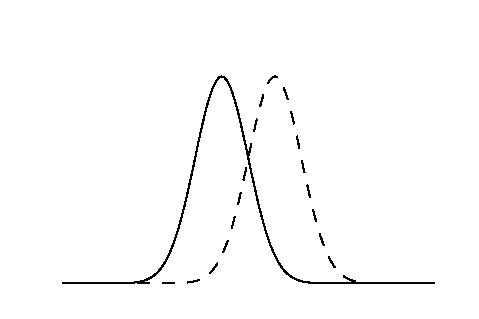
\includegraphics[height=1.5in]{figs/meanchange_lowvar}
\caption{ }
\end{subfigure}
~
\begin{subfigure}[b]{0.45\textwidth}
\centering
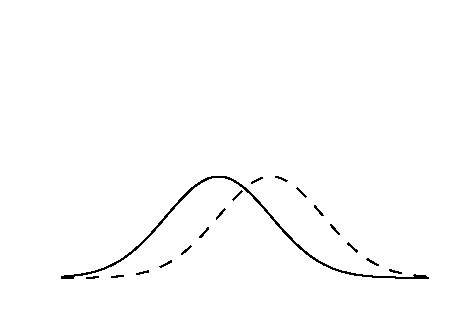
\includegraphics[height=1.5in]{figs/meanchange_highvar}
\caption{ }
\end{subfigure}
\caption{
 Changing the mean of a Gaussian by a fixed amount (from solid to
 dotted curve)
can have more impact
when the (shared) variance is small (as in a)
compared to when the variance is large (as in b).
Hence the impact (in terms of prediction accuracy)
of a change to $\mu$
depends on where the optimizer is in
$(\mu,\sigma)$ space.
\figtaken{Figure 3 of \citep{Honkela2010}, reproduced from 
\citep{ValpolaPhD}.}
\figthanks{Antti Honkela}.
}
\label{fig:honkelaGaussians}
\end{figure}

The key to NGD is to measure the notion of distance
between two probability distributions
in terms of the KL divergence.
This can be approximated in terms of
the \keywordDef{Fisher information matrix}  (FIM).
In particular, for any given input $\xdata$,
we have
\be
  \KLpq{p_{\params}(\vy|\xdata)}{p_{\params+\vdelta}(\vy|\xdata)}
  \approx
\half \vdelta^\trans \vFisher_{\xdata} \vdelta
\ee
where $\vFisher_{\xdata}$ is the FIM
\be
\vFisher_{\xdata}(\params)
= -\expectQ{\nabla^2 \log p_{\params}(\vy|\xdata)}{p_{\params}(\vy|\xdata)}
= \expectQ{(\nabla \log p_{\params}(\vy|\xdata))
(\nabla \log p_{\params}(\vy|\xdata))^\trans}{p_{\params}(\vy|\xdata)}
\ee
We  now replace the Euclidean distance
between the parameters,
$d(\vtheta_k, \vtheta_{k+1}) = ||\vdelta||_2^2$,
with 
\be
d(\vtheta_k, \vtheta_{k+1})
= \vdelta^\trans \vFisher_k \vdelta_k
\ee
where $\vdelta = \vtheta_{k+1}-\vtheta_k$
and $\vFisher_k = \vFisher_{\vx}(\vtheta_k)$
for a randomly chosen input $\vx$.
This gives rise to the following constrained
optimization problem:
\be
\vdelta_k = \argmin_{\vdelta}
\hat{\loss}_k(\vtheta_k + \vdelta) \myst
\vdelta^\trans \vFisher_k \vdelta \leq \epsilon
\ee
If we replace the constraint with a Lagrange multiplier,
we get the unconstrained objective:
\be
J_k(\vdelta) = \loss(\vtheta_k) + \vg_k^\trans \vdelta
+ \lr_k \vdelta^\trans \vFisher_k \vdelta 
\ee
Solving $J_k(\vdelta)=0$ gives the update
\be
\vdelta =  -\lr_k \vFisher_k^{-1} \vg_k
\ee
The term $\vFisher^{-1} \vg$
is called the \keywordDef{natural gradient}.
This is equivalent to  a preconditioned gradient update,
where we use the inverse FIM as a preconditioning matrix.
We can compute  the (adaptive) learning rate using
\be
\eta_k = \sqrt{\frac{\epsilon}{\vg_k^\trans \vF_k^{-1} \vg_k}}
\ee


Computing the FIM can be hard.
A simple approximation is to replace
the model's distribution with the empirical distribution.
In particular, define
 $\pemp(\xdata,\vy) = \frac{1}{N} \sum_{n=1}^N \delta_{\xdata_n}(\xdata) \delta_{\vy_n}(\vy)$,
$\pemp(\xdata) = \frac{1}{N} \sum_{n=1}^N \delta_{\xdata_n}(\xdata)$
and
$p_{\vtheta}(\vx,\vy) =  \pemp(\vx) p(\vy|\vx,\vtheta)$.
Then we can compute the \keywordDef{empirical Fisher}
\citep{Martens2016Thesis}
as follows:
\begin{align}
\vFisher(\vtheta) &= \expectQ{
\nabla \log p(\vy|\xdata,\params)
\nabla \log p(\vy|\xdata,\params)^\trans}
{p_{\vtheta}(\vx,\vy)} \\
 &\approx
\expectQ{
\nabla \log p(\vy|\xdata,\params)
\nabla \log p(\vy|\xdata,\params)^\trans}
{\pemp(\vx,\vy)} \\
&=
\frac{1}{|\data|}
\sum_{(\xdata,\vy) \in \data}
\nabla \log p(\vy|\xdata,\params)
\nabla \log p(\vy|\xdata,\params)^\trans
\end{align}

\subsubsection{Natural actor critic}

To apply NGD to RL, we can adapt
the A2C algorithm in \cref{algo:AC}.
In particular, define
\be
\vg_{kt} = \nabla_{\vtheta_k} A_t \log \pi_{\vtheta}(\va_t|\vs_t)
\ee
where $A_t$ is the advantage function at step $t$
of the random trajectory generated by the policy
at iteration  $k$.
Now we compute
\be
\vg_k = \frac{1}{T} \sum_{t=1}^T \vg_{kt},
\;
\vF_k = \frac{1}{T} \sum_{t=1}^T \vg_{kt} \vg_{kt}^\trans
\label{eqn:NACfisher}
\ee
and compute
$\vdelta_{k+1} = -\lr_k \vF_k^{-1} \vg_k$.
This approach is called \keywordDef{natural policy gradient}
\citep{Kakade2001,Rajeswaran2017}.

We can compute $\vF_k^{-1} \vg_k$ without having
to invert $\vF_k$ by using the conjugate gradient method,
where each CG step uses efficient
methods for Hessian-vector products \citep{Pearlmutter1994}.
This is called
\keywordDef{Hessian free optimization}  \citep{Martens2010}.
Similarly, we can efficiently compute
$\vg_k^\trans (\vF_{k}^{-1} \vg_k)$.

As a more accurate alternative
to the empirical Fisher,
\citep{Martens2015kfac} propose
the \keywordDef{KFAC} method,
which stands for ``Kronecker factored approximate curvature'';
this approximates the FIM of a DNN as a block diagonal
matrix, where each block is a Kronecker product
of two small matrices.
This was applied to policy gradient learning in \citep{Wu2017kfac}.


\eat{
\section{Bound optimization methods}

In this section, we describe methods that
aim to monotonically improve the performance of the policy
at each step,
similar to other \keywordDef{bound optimization} methods\footnote{
%
Bound optimization is also called \keywordDef{MM},
for majorize then maximize/minimize.
See \citep{Hunter04} for a tutorial.
} %
such as EM.
}

\section{Policy improvement methods}
\label{sec:polImprovement}
\label{sec:policyImprovement}

In this section, we discuss methods that try to monotonically
improve performance of the policy at each step,
rather than just following the gradient,
which can result in a high variance estimate
where performance can increase or decrease at each step.
These are called \keywordDef{policy improvement} methods.
Our presentation is based on \cite{Queeney2024}.

\subsection{Policy improvement lower bound}

We start by stating a useful result from
\citep{Achiam2017}.
Let $\pi_k$ be the current policy at step $k$,
and let $\pi$ be any other policy (e.g., a candidate new one).
Let  $\statdistpolk$ be the normalized
discounted state visitation distribution for $\policy_k$,
defined in \cref{eqn:statdistpol}.
Let $A^{\pi_k}(s,a) = Q^{\pi_k}(s,a)-V^{\pi_k}(s)$
be the advantage function.
Finally, let the total variation distance
between two distributions be
given by
\be
\text{TV}(p,q) \defeq \half ||\vp-\vq||_1
= \half \sum_s |p(s) - q(s)| 
\ee
Then one can show \citep{Achiam2017} that
\be
J(\pi) - J(\pi_k)
\geq
  \frac{1}{1-\gamma}
\underbrace{
 \expectQ{
  \frac{\pi(a|s)}{\pi_k(a|s)}
  A^{\pi_k}(s,a)}{\statdistpolk(s) \policy_k(a|s)}
}_{L(\pi,\pi_k)}
-
  \frac{2 \gamma C^{\pi,\pi_k}}{(1-\gamma)^2}
  \expectQ{\text{TV}(\pi(\cdot|s),\pi_k(\cdot|s))}{\statdistpolk(s)}
\label{eqn:Jlowerbound}
  \ee
where
$C^{\pi,\pi_k} = \max_s |\expectQ{A^{\pi_k}(s,a)}{\pi(a|s)}|$.
In the above, $L(\pi,\pi_k)$ is a  surrogate objective,
and the second term is a penalty term.

If we can optimize this lower bound (or a stochastic approximation,
based on samples from the current policy $\pi_k$),
we can guarantee monotonic policy improvement (in expectation)
at each step.
We will replace this objective with a trust-region update
that is easier to optimize:
\be
\pi_{k+1} = \argmax_{\pi} L(\pi,\pi_k)
\myst   \expectQ{\text{TV}(\pi,\pi_k)(s)}{\statdistpolk(s)} \leq
\epsilon
\label{eqn:polImprovementBound}
\ee
The constraint bounds the worst-case performance decline at each
update.
The overall procedure becomes an approximate policy improvement
method.
There are various ways of implementing the above method in practice,
some of which we discuss below.
(See also \citep{Grudzien2022}, who propose a framework
called \keywordDef{mirror learning},
that justifies these ``approximations'' as in fact being
the optimal thing to do for a different kind of objective.)



\subsection{Trust region policy optimization (TRPO)}
\label{sec:TRPO}



In this section, we describe
the \keywordDef{trust region policy optimization}
(\keywordDef{TRPO}) method of \citep{TRPO}.
This implements an approximation to \cref{eqn:polImprovementBound}.
First, it leverages the fact that if
\be
\expectQ{\KLpq{\pi_k}{\pi}(s)}{\statdistpolk(s)} \leq \delta
\ee
then $\pi$ also satisfies the TV constraint
with $\delta=\frac{\epsilon^2}{2}$.
Next it considers a first-order expansion of the surrogate objective
to get
\be
L(\pi,\pi_k)
=
 \expectQ{
  \frac{\pi(a|s)}{\pi_k(a|s)}
  A^{\pi_k}(s,a)}{\statdistpolk(s) \policy_k(a|s)}
\approx \vg_k^\trans (\vtheta-\vtheta_k)
\ee
where $\vg_k = \nabla_{\vtheta} L(\pi_{\vtheta},\pi_k)|_{\vtheta_k}$.
Finally it considers a second-order expansion of the KL term
to get the approximate constraint
\be
\expectQ{\KLpq{\pi_k}{\pi}(s)}{\statdistpolk(s)}
\approx \half (\vtheta-\vtheta_k)^\trans \vF_k (\vtheta-\vtheta_k)
\ee
where $\vF_k = \vg_k \vg_k^\trans$ is an approximation to
the Fisher information matrix
(see \cref{eqn:NACfisher}).
We then use the update
\be
\vtheta_{k+1} = \vtheta_k + \eta_k \vv_k
\ee
where $\vv_k = \vF_k^{-1} \vg_k$ is the natural gradient,
and the step size is initialized to
$\eta_k = \sqrt{\frac{2 \delta}{\vv_k^\trans \vF_k \vv_k}}$.
(In practice we compute $\vv_k$ by approximately
solving the linear system $\vF_k \vv = \vg_k$
using conjugate gradient methods,
which just require matrix vector multiplies.)
We then use a backtracking line search procedure
to ensure the trust region is satisfied.

\eat{
We start with a useful fact that relate
the policy values of two arbitrary policies
\citep{Kakade2002RL}:
\begin{align}
\polval(\policy')-\polval(\policy)
=  \expectQ{\expectQ{\Apol(s,a)}{\policy'(a|s)}}
{\statmeasure_{\policy'}(s)}
 \label{eqn:PolicySwitchThm}
\end{align}
where $\policy$ can be interpreted as the current policy during policy optimization, and $\policy'$ a candidate new policy (such as the greedy policy wrt $\Qpol$).
As in the policy improvement theorem
(\cref{sec:policyIteration}),
if $\expectQ{\Apol(s,a)}{\policy'(a|s)} \ge 0$ for all $s$,
then $\polval(\policy') \ge \polval(\policy)$.
However, we cannot ensure this condition to hold
when function approximation is used,
as such a uniformly improving policy $\policy'$
may not be representable by our parametric family.
Therefore, nonnegativity of \cref{eqn:PolicySwitchThm}
is not easy to ensure.


One way to ensure monotonic improvement of
$\polval$ is to improve the policy conservatively.
Let us define
\begin{align}
\polvallin( \policy')
 \defeq  \expectQ{\expectQ{\Apol(s,a)}{\policy'(a|s)}}{\statmeasure_{\policy}(s)}
 = \expectQ{\frac{\policy'(a|s)}{\policy(a|s)}
   \Apol(s,a)}{\statmeasure_{\policy}(s)\policy(a|s)}
 \label{eqn:polvalLin}
\end{align}
In the above,
we have switched the state distribution from
$\statmeasure_{\policy'}$ in \cref{eqn:PolicySwitchThm}
to $\statmeasure_{\policy}$.
In \citep{TRPO} they show that
we have  we have the following lower bound on the improvement:
\be
J(\pi') - J(\pi) \geq L(\pi') - C \max_s \KLpq{\pi(a|s)}{\pi'(a|s)}
\label{eqn:JlowerBound}
\ee
where $C$  is a constant.
We can approximate the max over states with an expectation,
to get the  following constrained optimization problem:
\begin{align}
\label{eqn:TRPOconstr}
\argmax_{\policy'}
 \polvallin(\policy')
 \myst
 \expectQ{\KLpq{\policy(\cdot|s)}{\policy'(\cdot|s)}}
         {\statmeasure_{\policy}(s)} \leq \delta
\end{align}
for some threshold $\delta>0$.
We can then approximate the KL term with the Fisher information
matrix, as in \cref{sec:NGD}.
This gives the update
\be
\vtheta_{k+1} = \vtheta_k + \lr_k \vF(\vtheta_k)^{-1}
  \nabla_{\vtheta} L(\vtheta)\vert_{\vtheta_k}
  \ee
 We  can compute $\lr_k$ using a linesearch procedure:
 we start with largest value for $\lr_k$ allowed by the KL constraint,
 and reduce it until
 the lower bound is positive.
}


\subsection{Proximal Policy Optimization (PPO)}
\label{sec:PPO}

In this section, we describe the
the \keywordDef{proximal policy optimization}
or \keywordDef{PPO} method of \citep{PPO},
which is a simplification of TRPO.
%Note that PPO does not guarantee monotonic improvement,
%but can be modified to do so
%\citep{Wang2019PPO}.
%The blog post at \url{https://vitalab.github.io/article/2020/01/14/Implementation\_Matters.html}
%argues that the benefits of PPO over TRPO follow more from
%code-level optimizations than the objective itself.
%See  \url{https://iclr-blog-track.github.io/2022/03/25/ppo-implementation-details/}


We start by noting the following result:
\be
\expectQ{\text{TV}(\pi,\pi_k)(s)}{\statdistpolk(s)}
= \half \expectQ{| \frac{\pi(a|s)}{\pi_k(a|s)} - 1 |}
{(s,a) \sim \statdistpolk}
\ee
This holds provided the support of $\pi$ is contained
in the support of $\pi_k$ at every state.
We then use the following update:
\be
\pi_{k+1} = \argmax_{\pi} 
\expectQ{
  \min\left( \rho_k(s,a)  A^{\pi_k}(s,a),
  \tilde{\rho}_k(s,a)  A^{\pi_k}(s,a)
  \right)}{(s,a) \sim \statdistpolk}
\ee
where $\rho_k(s,a) = \frac{\pi(a|s)}{\pi_k(a|s)}$
is the likelihood ratio, and
$\tilde{\rho}_k(s,a)= \text{clip}(\rho_k(s,a), 1-\epsilon,
1+\epsilon)$,
where $\text{clip}(x,l,u) = \min(\max(x,l),u)$.
\eat{
We start by considering the following unconstrained objective,
based on \cref{eqn:JlowerBound}:
\begin{align}
  \polval(\policy') = \polvallin(\policy')
  - \beta\expectQ{\KLpq{\policy(\cdot|s)}{\policy'(\cdot|s)}}
  {\statmeasure_{\policy}(s)}
\end{align}
where
\begin{align}
\polvallin( \policy')
 = \expectQ{\frac{\policy'(a|s)}{\policy(a|s)}
   \Apol(s,a)}{\statmeasure_{\policy}(s)\policy(a|s)}
\end{align}
Unfortunately, the likelihood ratio
\be
l(s,a) = \frac{\pi'(a|s)}{\pi(a|s)}
\ee
which is needed to compute $\polvallin(\policy')$
might become very large or small, if $\pi'$ deviates too much
from $\pi$. To ensure stability we can replace it with
\be
\tilde{l}(s,a) = 
\text{clip}(r(s,a;\vtheta), 1-\epsilon, 1+\epsilon)
\ee
which ensures $|l(s,a;\vtheta) - 1| \leq \epsilon$.
Furthermore, we can drop the KL penalty and just optimize
\be
\polval(\vtheta) = \expect{\min(l(s,a;\vtheta) \Apol(s,a), \;\;
\tilde{l}(s,a;\vtheta) \Apol(s,a))}
\ee
}
See \citep{Grudzien2022} for a theoretical justification
for these simplifications.
Furthermore,
this can be modified to ensure monotonic
improvement as discussed in \citep{Wang2019PPO},
making it a true bound optimization method.


Some pseudocode for PPO (with GAE)
is given in \cref{algo:PPO}.
It is basically identical to the AC code in \cref{algo:AC},
except the policy loss has the form
$\min(\rho_t A_t, \tilde{\rho}_t A_t)$
instead of
$A_t \log \pi_{\vphi}(a_t|s_t)$,
and we perform multiple policy updates per rollout,
for increased sample efficiency.
For all the implementation details, see
\url{https://iclr-blog-track.github.io/2022/03/25/ppo-implementation-details/}.


\begin{algorithm}
\dontprintsemicolon
\caption{PPO  with GAE}
\label{algo:PPO}
Initialize  parameters $\vphi$, 
environment state $s$\\
\For{iteration $k=1,2,\ldots$}
{
  $(\tau,s) = \text{rollout}(s, \pi_{\vphi})$ \\
  $(s_1,a_1,r_1,\ldots,s_T)= \tau$ \\
  $v_{t} = V_{\vphi}(s_{t}) \; \text{for } t=1:T$ \\
  $(A_{1:T}, \targetV_{1:T}) = \text{GAE}(r_{1:T}, v_{1:T}, \gamma, \lambda)$
  \\
  $\vphi_{\old} \assign \vphi$ \\
  \For{$m=1:M$}{
  $\rho_{t} = \frac{\pi_{\vphi}(a_t|s_t)}{\pi_{\vphi_{\old}}(a_t|s_t)}
  \; \text{for } t=1:T$  \\
  $\tilde{\rho}_t = \text{clip}(\rho_t) \text{ for } t=1:T$ \\
  $\loss(\vphi) = \frac{1}{T}\sum_{t=1}^T \left[
    \lambda_{TD} (V_{\vphi}(s_t) - \targetV_t)^2
    -\lambda_{PG} \min(\rho_t A_t, \tilde{\rho}_t A_t)
    -\lambda_{ent} \entropy(\pi_{\vphi}(\cdot|s_t)) \right]$ \\
  $\vphi := \vphi -  \lr \nabla_{\vphi} \loss(\vphi)$ \\
  }
}
\end{algorithm}


\eat{
\begin{algorithm}
\dontprintsemicolon
\caption{PPO with $1$-step critic}
\label{algo:PPO}
Initializeparameters $\vphi$,
environment state $s$\\
\Repeat{converged}
{
  $(\tau,s) = \text{rollout}(s, \pi_{\vtheta})$ \\
  \For{$k=1:K$}{
    $\vphi_{\old}=\vphi$ \\
    $\vphi = \text{PPO-step}(\tau, \vphi,  \vphi_{\old})$ \\
    }
}
.\\
$\text{def PPO-step}(\tau, \vphi, \vphi_{\old})$: \\
Let $(s_0,a_0,r_0,\ldots,s_T)=\tau$ \\
\For{$t=0:T-1$}{
  $G_t = r_{t+1} + \gamma V_{\vphi}(s_{t+1})$ \\
  $A_t = \stopgrad(G_t - V_{\vphi}(s_t))$ \\
  $r_t = \frac{\pi_{\vphi}(a_t|s_t)}{\pi_{\vphi_{\old}}(a_t|s_t)}$
  \\
  $\tilde{r}_t = \text{clip}(r_t)$ \\
}
$\loss = \frac{1}{T} \sum_t \left[
  \lambda_V (V_{\vphi}(s_t) - G_t)^2
  -\lambda_{\pi} \min(r_t A_t, \tilde{r}_t A_t)
  -\lambda_{ent} \entropy(\pi_{\vphi}(\cdot|s_t)) \right]$ \\
$\vphi \assign \vphi - \lr \nabla \loss$\\
       Return $\vphi$
\end{algorithm}
}

% https://github.com/luchris429/purejaxrl/blob/main/purejaxrl/ppo.py#L173
% https://github.com/snu-mllab/Achievement-Distillation/blob/main/achievement_distillation/model/ppo.py#L107

\eat{
\begin{algorithm}
\dontprintsemicolon
\caption{PPO with $1$-step critic}
\label{algo:PPO}
Initialize actor parameters $\vtheta$, critic parameters $\vw$,
environment state $s$\\
\Repeat{converged}
{
  $(\tau,s) = \text{rollout}(s, \pi_{\vtheta})$ \\
  \For{$k=1:K$}{
    $\vtheta_{\old}=\vtheta$ \\
    $(\vtheta, \vw) = \text{PPO-step}(\vtheta, \vw, \tau, \vtheta_{\old})$ \\
    }
}
.\\
$\text{def PPO-step}(\vtheta,\vw,\tau,\vtheta_{\old})$: \\
Let $(s_0,a_0,r_0,\ldots,s_T)=\tau$ \\
\For{$t=0:T-1$}{
  $Q_t = r_{t+1} + \gamma V_{\vw}(s_{t+1})$ \\
  $A_t = \stopgrad(Q_t - V_{\vw}(s_t))$ \\
  $r_t = \frac{\pi_{\vtheta}(a_t|s_t)}{\pi_{\vtheta_{\old}}(a_t|s_t)}$
  \\
  $\tilde{r}_t = \text{clip}(r_t)$ \\
}
$\loss_{\vw} = \frac{1}{T} \sum_t (V_{\vw}(s_t) - \stopgrad(Q_t))^2$ \\
$\loss_{\vtheta} = -\frac{1}{T} \sum_t 
\min(r_t A_t, \tilde{r}_t A_t)$ \\
$\vw \assign \vw - \lr_{\vw} \nabla \loss_{\vw}$\\
$\vtheta \assign \vtheta - \lr_{\vtheta} \nabla \loss_{\vtheta}$ \\
       Return $(\vtheta,\vw)$
\end{algorithm}
}



\subsection{VMPO}
\label{sec:MPO}
\label{sec:VMPO}


In this section, we discuss
the \keywordDef{VMPO} algorithm of \citep{VMPO},
which is an on-policy extenson of the earlier
on-policy \keywordDef{MPO} algorithm (MAP policy optimization)
from \citep{Abdolmaleki2018}.
It was originally explained in terms of ``control as inference''
(see \cref{sec:inferRL}),
but we can also view it as
a  contrained policy improvement method,
based on   \cref{eqn:polImprovementBound}.
In particular, VMPO leverages the fact that if
\be
\expectQ{\KLpq{\pi}{\pi_k}(s)}{\statdistpolk(s)} \leq \delta
\ee
then $\pi$ also satisfies the TV constraint
with $\delta=\frac{\epsilon^2}{2}$.

Note that here the KL is reversed compared to TRPO
in \cref{sec:TRPO}.
This new version will encourage $\pi$
to be mode-covering, so it will naturally
have high entropy, which can result in improved robustness.
Unfortunately, this kind of KL is harder to compute,
since we are taking expectations wrt the unknown distribution $\pi$.

To solve this problem, VMPO adopts an EM-type approach.
In the E step, we compute a non-parametric version
of the state-action distribution given by the unknown
new policy:
\be
\psi(s,a) = \pi(a|s) \statdistpolk(s)
\ee
The optimal new distribution is given by
\be
\psi_{k+1} = \argmax_{\psi}
\expectQ{A^{\pi_k}(s,a)}{\psi(s,a)}
\myst \KLpq{\psi}{\psi_k} \leq \delta
\ee
where
$\psi_k(s,a) = \pi_k(a|s) \statdistpolk(s)$.
The solution to this  is
\begin{align}
  \psi_{k+1}(s,a) &=  \statdistpolk(s) \pi_k(a|s) w(s,a) \\
  w(s,a) &= \frac{\exp(A^{\pi_k}(s,a)/\lambda^*)}{Z(\lambda^*)} \\
  Z(\lambda) &= \expectQ{\exp(A^{\pi_k}(s,a)/\lambda)}{(s,a)\sim
    \statdistpolk} \\
  \lambda^* &= \argmin_{\lambda \geq 0} \lambda \delta + \lambda \log Z(\lambda)
  \end{align}
In the M step, we project this target distribution back onto the space
of parametric policies, while satisfying the KL trust region
constraint:
\be
\pi_{k+1} = \argmax_{\pi}
\expectQ{w(s,a) \log \pi(a|s)}{(s,a) \sim \statdistpolk}
\myst \expectQ{\KLpq{\psi_k}{\psi}(s)}{\statdistpolk} \leq \delta
\ee


\section{Off-policy methods}
\label{sec:offPolicy}
\label{sec:offpolicy}


In many cases, it is useful to train a policy
using data collected from a distinct
\keywordDef{behavior policy}
$\behavior(a|s)$ that is
not the same as the \keywordDef{target policy} $\policytgt(a|s)$
that is being learned.
For example, this could be data collected
from earlier trials or parallel workers
(with different parameters $\vtheta'$)
and stored in a \keywordDef{replay buffer},
or it could be \keywordDef{demonstration data} from human experts.
This is known as \keywordDef{off-policy RL},
and can be much more sample efficient than the on-policy 
methods we have discussed so far, since these methods
can use data from multiple sources.
However, off-policy methods are more complicated,
as we will explain below.

The basic difficulty  is that the target policy  that we want to learn
may want to try an action in a state that has
not been experienced before in the existing data,
so there is no way to predict the outcome of this new $(s,a)$
pair.
In this section, we tackle this problem by assuming
that the  target policy is not too different from the behavior policy,
so that the ratio $\policytgt(a|s)/\policybeh(a|s)$
is bounded, which allows us to use methods based on importance
sampling.
%(In particular, this means that the behavior
%policy must have broad enough support that it covers the target.)
In the online learning setting, we can ensure this property
by using conservative incremental updates to the policy.
%as we discuss in \cref{sec:offpolPolImprovement}.
Alternatively we can use policy gradient methods
with various regularization methods, as we discuss below.

In \cref{sec:offlineRL}, we discuss offline RL,
which is an extreme instance of off-policy RL where we
have a fixed behavioral dataset, possibly generated from an unknown
behavior policy,
and can never collect any new data.



\subsection{Policy evaluation using importance sampling}
\label{sec:offpolicyRL-IS}

Assume we have a dataset of the form
$\data = \{\traj^{(i)}\}_{1 \le i \le n}$, where each trajectory is a sequence
$\traj^{(i)}=(s_0^{(i)},a_0^{(i)},r_0^{(i)},s_1^{(i)}\ldots)$,
where the actions are sampled according to a behavior policy
$\policybeh$, and
the reward and next states are sampled
according to the reward and transition models.
We want to use this offline dataset to evaluate the performance of some
target policy $\policytgt$;
this is called \keywordDef{off-policy policy evaluation} or \keywordDef{OPE}.
If the trajectories $\traj^{(i)}$ were sampled from $\policytgt$.
we could use the standard Monte Carlo estimate:
\begin{align}
  \hat{J}(\policytgt)
\defeq \frac{1}{n} \sum_{i=1}^n  \sum_{t=0}^{T-1} \gamma^t r_t^{(i)}
\end{align}
However, since the trajectories are sampled from $\policybeh$,
we use \keywordDef{importance sampling} (IS)
to correct for the distributional mismatch,
as first proposed in \citep{Precup2000}.
This gives
\begin{align}
\label{eqn:offpolicyrl-basicis}
  \polvalis(\policytgt)
  \defeq \frac{1}{n} \sum_{i=1}^n
  \frac{p(\traj^{(i)}|\policytgt)}{p(\traj^{(i)}|\policybeh)}
  \sum_{t=0}^{T-1} \gamma^t r_t^{(i)}
\end{align}
It can be verified that $\expectQ{\polvalis(\policytgt)}{\policybeh}
= \polval(\policytgt)$, that is, $\polvalis(\policytgt)$ is \keywordDef{unbiased},
provided that $p(\traj|\policybeh)>0$
whenever $p(\traj|\policytgt)>0$.
The \keywordDef{importance ratio},
$\frac{p(\traj^{(i)}|\policytgt)}{p(\traj^{(i)}|\policybeh)}$,
is used to compensate for the fact that
the data is sampled from $\policybeh$ and not $\policytgt$.
It can be simplified as follows:
\begin{align}
\label{eqn:offpolicyrl-isratio}
\frac{p(\traj|\policytgt)}{p(\traj|\policybeh)}
= \frac{p(s_0) \prod_{t=0}^{T-1} \policytgt(a_t|s_t) \ptran(s_{t+1}|s_t,a_t) \preward(r_t|s_t,a_t,s_{t+1})}{p(s_0) \prod_{t=0}^{T-1} \policybeh(a_t|s_t) \ptran(s_{t+1}|s_t,a_t) \preward(r_t|s_t,a_t,s_{t+1})}
= \prod_{t=0}^{T-1} \frac{\policytgt(a_t|s_t)}{\policybeh(a_t|s_t)}
\end{align}
This simplification makes it easy to apply IS,
as long as the target and behavior policies are known.
(If the behavior policy is unknown,
we can estimate it from $\data$,  and replace $\policybeh$
by its estimate $\hat{\policybeh}$.
For convenience, define the
\keywordDef{per-step importance ratio} at time $t$ by
\be
\psiRatio_t(\traj) \defeq \policytgt(a_t|s_t) / \policybeh(a_t|s_t)
\ee
We can reduce the variance of the estimator
by noting that the reward $r_t$ is independent of the trajectory
beyond time $t$.
This leads to a \keywordDef{per-decision importance sampling} variant:
\begin{align}
\label{eqn:offpolicyrl-pdis}
  \polvalpdis(\policytgt)
  \defeq \frac{1}{n} \sum_{i=1}^n \sum_{t=0}^{T-1}
  \prod_{t' \le t} \psiRatio_{t'}(\traj^{(i)}) \gamma^t r_t^{(i)}
\end{align}

\subsection{Off-policy actor critic methods}
\label{sec:offPolicyPG}

In this section, we discuss how to extend actor-critic
methods to work with off-policy data.

\subsubsection{Learning the critic using V-trace}
\label{sec:Vtrace}

In this section
we build on \cref{sec:offpolicyRL-IS} to develop a practical method,
known as \keywordDef{V-trace} \citep{Espeholt2018},
to estimate the value function for a target policy
using off-policy data.
(This is an extension of the earlier
\keywordDef{Retrace} algorithm \citep{Munos16},
which estimates the $Q$ function using off-policy data.)

First consider the $n$-step target value for $V(s_i)$
in the on-policy case:
\begin{align}
  V_i  &= V(s_i)
  + \sum_{t=i}^{i+n-1} \gamma^{t-i} r_t + \gamma^n V(s_{i+n}) \\
  &= V(s_i)
  + \sum_{t=i}^{i+n-1} \gamma^{t-i}
  \underbrace{(r_t + \gamma V(s_{t+1}) - V(s_t))}_{\delta_t}
\end{align}
where we define $\delta_t  = (r_t + \gamma V(s_{t+1}) - V(s_t))$
as the TD error at time $t$.
To extend this to the off-policy case, we use the per-step
importance ratio trick. However, to bound the variance
of the estimator, we truncate the IS weights.
In particular, we define
\begin{align}
  c_t &= \min\left(\overline{c},
  \frac{\policytgt(a_t|s_t)}{\policybeh(a_t|s_t)} \right),
  \;
  \rho_t = \min\left(\overline{\rho},
  \frac{\policytgt(a_t|s_t)}{\policybeh(a_t|s_t)} \right) 
\end{align}
where $\overline{c}$ and $\overline{\rho}$
are hyperparameters.
We then define the V-trace target value for $V(s_i)$ as
\begin{align}
  v_i
  &= V(s_i)
  + \sum_{t=i}^{i+n-1} \gamma^{t-i} \left( \prod_{t'=i}^{t-1} c_{t'}
  \right)   \rho_t \delta_t
\end{align}
Note that we can compute these targets recursively using
\be
v_i = V(s_i) + \rho_i  \delta_i + \gamma c_i (v_{i+1} - V(s_{i+1}))
\ee

The product of the weights $c_i \ldots c_{t-1}$ (known as the ``trace'')
measures how much a temporal difference $\delta_t$
at time $t$ impacts the update of the value function
at earlier time $i$.
If the policies are very different, the variance of this product
will be large. So the truncation parameter $\overline{c}$
is used to reduce the variance.
In  \citep{Espeholt2018}, they find $\overline{c}=1$ works best.

The use of the target $\rho_t \delta_t$  rather than $\delta_t$
means we are evaluating the value function for a policy
that is somewhere between $\policybeh$ and $\policytgt$.
For $\overline{\rho}=\infty$ (i.e., no truncation),
we converge to the value function $V^{\policytgt}$,
and for $\overline{\rho} \ra 0$,
we converge to the value function $V^{\policybeh}$.
In  \citep{Espeholt2018}, they find $\overline{\rho}=1$ works best.

Note that if $\overline{c}=\overline{\rho}$,
then $c_i=\rho_i$. This gives rise to the simplified form
\begin{align}
  v_t
  &= V(s_t)
  + \sum_{j=0}^{n-1} \gamma^{j} \left( \prod_{m=0}^{j} c_{t+m}
  \right)   \delta_{t+j}
  \label{eqn:Vtrace}
\end{align}

We can use the above V-trace targets to learn an approximate
value function by minimizing the usual $\ell_2$ loss:
\be
\loss(\vw) = \expectQ{(v_t - V_{\vw}(s_t))^2}{t \sim \data}
\ee
the gradient of which has the form
\be
\nabla \loss(\vw) = 2 \expectQ{(v_t - V_{\vw}(s_t))
  \nabla_{\vw}  V_{\vw}(s_t)}{t \sim \data}
\ee


\subsubsection{Learning the actor}
\label{sec:offpolPG}

We now discuss how to update the actor
using an off-policy estimate of the policy gradient.
We start by defining the objective to be
the expected value of the new policy,
where the states are drawn from the behavior
policy's state distribution, but the actions
are drawn from the target policy:
\be
J_{\behavior}(\policy_{\vtheta})
= \sum_s \statdistbehave(s) \Vpol(s)
= \sum_s \statdistbehave(s) \sum_a \policy_{\vtheta}(a|s) \Qpol(s,a)
\label{eqn:offPolicyJ}
\ee
Differentiating this and
ignoring the term $\nabla_{\vtheta} \Qpol(s,a)$, as suggested by \citep{Degris2012},
gives a way to (approximately) estimate the
\keywordDef{off-policy policy-gradient}
using a one-step IS correction ratio:
\begin{align}
\nabla_{\vtheta}
 J_{\behavior}(\policy_{\vtheta})
  &\approx \sum_s \sum_a
  \statdistbehave(s) \nabla_{\vtheta} \policy_{\vtheta}(a|s) \Qpol(s,a) \\
  &= \expectQ{  \frac{\policy_{\vtheta}(a|s)}{\behavior(a|s)}
  \nabla_{\vtheta} \log \policy_{\vtheta}(a|s) \Qpol(s,a)}
  {\statdistbehave(s), \behavior(a|s)}
\end{align}

In practice, we can approximate $Q_{\pi}(s_t,a_t)$
by $q_t = r_t + \gamma v_{t+1}$,
where $v_{t+1}$ is the V-trace estimate for state $s_{t+1}$.
If we use $V(s_t)$ as a baseline, to reduce the variance,
we get the following gradient estimate for the policy:
\be
\nabla J(\vtheta) = \expectQ{
  \rho_t \nabla_{\vtheta} \log \pi_{\vtheta}(a_t|s_t)
  (r_t + \gamma v_t - V_{\vw}(s_t))}{t \sim \data}
\ee

We can also replace the 1-step IS-weighted TD error
$\rho_t (r_t + \gamma v_t - V_{\vw}(s_t))$
with an IS-weighted GAE value
by modifying the generalized advantage estimation method
in \cref{sec:GAE}.
In particular, we just need to define
$\lambda_t = \lambda \min(1, \rho_t)$.
We denote the IS-weighted GAE estimate  as $A_t^{\rho}$.\footnote{
  %
  For an implementation, see
  \url{https://github.com/google-deepmind/rlax/blob/master/rlax/\_src/multistep.py\#L39}
  }

\subsubsection{IMPALA}
\label{sec:IMPALA}

As an example of an off-policy AC method,
we consider
\keywordDef{IMPALA},
which stands for ``Importance Weighted Actor-Learning Architecture''.
\citep{Espeholt2018}.
This uses  shared parameters for the policy and value function
(with different output heads), and adds an entropy bonus
to ensure the policy remains stochastic.
Thus we end up with the following objective,
which is very similar to on-policy actor-critic
shown in \cref{algo:AC}:
\be
  \loss(\vphi) = \expectQ{
    \lambda_{TD} (V_{\vphi}(s_t) - v_t)^2
    -\lambda_{PG} A_t^{\rho} \log \pi_{\vphi}(a_t|s_t)
    -\lambda_{ent} \entropy(\pi_{\vphi}(\cdot|s_t))
  }{t \sim \data}
  \label{eqn:offpolAC}
  \ee
The only difference from standard A2C is that we need
to store the probabilities of each action,
$\policybeh(a_t|s_t)$, in addition to $(s_t,a_t,r_t,s_{t+1})$
in the dataset $\data$,
which can be used to compute $\rho_t$.
\citep{Espeholt2018} was  able to use this method to train 
a single agent (using a shared CNN and LSTM for both value and policy)
to play all 57 games at a high level.
Furthermore, they showed that their
method --- thanks to its off-policy corrections ---
outperformed the A3C method (a parallel version of A2C) in \cref{sec:A3C}.



 \eat{
The term $\frac{\policy_{\vtheta}(a|s)}{\behavior(a|s)}$
is an \keywordDef{importance sampling} correction term,
used to compensate for the fact that the data is sampled
from $\behavior$ and not $\policy$.
We require that  the support of the behavior
policy  is at least
as broad as the target policy,
so $\policy(a|s)>0 \implies \behavior(a|s)>0$.
Also,  to ensure the variance of the estimators is reasonable,
we require that $\behavior$ be close to $\policy$.
This can be problematic in cases where the behavioral
data is log data that is created offline by some other system.
See \cref{sec:offlineRL} for a discussion of such cases.
In online RL, we can ensure the new policy does not
differ too much from the old policy, using methods
such as TRPO (\cref{sec:TRPO}),
PPO (\cref{sec:PPO}) and MPO (\cref{sec:MPO}).
In  \cref{sec:DPG},
we discuss a way to avoid the need to compute the IS ratio.
}





\subsection{Off-policy policy improvement methods}
\label{sec:offpolPolImprovement}

So far we have focused on  actor-critic methods.
However, policy improvement methods, such as PPO,
are often preferred to AC methods,
since they monotonically improve the objective.
In  \citep{Queeney2021} they propose
one way to extend PPO to the off-policy case.
This method was generalized in  \cite{Queeney2024}
to cover a variety of policy improvement algorithms,
including TRPO and VMPO.
We give a brief summary below.

The key insight is to realize that we can generalize
the lower bound in \cref{eqn:Jlowerbound}
to any reference policy 
\be
J(\pi) - J(\pi_k)
\geq
  \frac{1}{1-\gamma}
 \expectQ{
  \frac{\pi(a|s)}{\policyref(a|s)}
  A^{\pi_k}(s,a)}{\statdistpolref(s) \policy_k(a|s)}
-
  \frac{2 \gamma C^{\pi,\pi_k}}{(1-\gamma)^2}
  \expectQ{\text{TV}(\pi(\cdot|s),\policyref(\cdot|s))}{\statdistpolref(s)}
  \ee
The reference policy can be any previous policy,
or a convex combination of them.
In particular, if $\pi_k$ is the current policy,
we can consider the reference policy to be
$\policyref = \sum_{i=1}^M \nu_i \pi_{k-i}$,
where $0 \leq \nu_i \leq 1$
and $\sum_i \nu_i = 1$ are mixture weights.
We can approximate the expectation
by sampling  from the  replay buffer,
which contains samples from older policies.
That is, $(s,a) \sim \statdistpolref$
can be implemented by $i \sim \nu$
and $(s,a) \sim \statdistpolki$.

To compute the advantage function $A^{\pi_k}$
from off policy data, we can adapt the V-trace
method of \cref{eqn:Vtrace} to get
\begin{align}
  A_{\ttrace}^{\pi_k}(s_t,a_t)
  &= \delta_t
  + \sum_{j=0}^{n-1} \gamma^{j} \left( \prod_{m=1}^{j} c_{t+m}
  \right)   \delta_{t+j}
\end{align}
where
$\delta_t = r_t + \gamma V(s_{t+1}) - V(s_t)$,
and
$c_t = \min\left(\overline{c},
\frac{\pi_k(a_t|s_t)}{\pi_{k-i}(a_t|s_t)} \right)$
is the truncated importance sampling ratio.


To compute the TV penalty term from off policy data,
we need to choose between the PPO (\cref{sec:PPO}),
VMPO (\cref{sec:VMPO})
and TRPO (\cref{sec:TRPO}) approach.
We discuss each of these cases below.

\subsubsection{Off-policy PPO}

The simplest is to use off-policy PPO, which gives an update of the
following form (known as \keywordDef{Generalized PPO}):
\be
\pi_{k+1} = \argmax_{\pi} \expectQ{
  \expectQ{
    \min( \rho_{k-i}(s,a) A^{\pi_k}(s,a),
    \tilde{\rho}_{k-i}(s,a) A^{\pi_k}(s,a) )
  }{(s,a) \sim \statdistpolki}
  }{i \sim \nu}
\ee
where $\rho_{k-i}(s,a)=\frac{\pi(a|s)}{\pi_{k-i}(a|s)}$
and
$\tilde{\rho}_{k-i}(s,a)=\text{clip}(\frac{\pi(a|s)}{\pi_{k-i}(a|s)},l,u)$,
where $l=\frac{\pi_k(a|s)}{\pi_{k-i}(a|s)} - \epsilon$
and $u=\frac{\pi_k(a|s)}{\pi_{k-i}(a|s)} + \epsilon$.
(For other off-policy variants of PPO,
see e.g., \citep{Meng2023,Li2024R3}.)

\subsubsection{Off-policy VMPO}

%For details on the off-policy version of TRPO,
%please see \cite{Queeney2024}.
For an off-policy version of VMPO,
see  the original \keywordDef{MPO} method of \citep{Abdolmaleki2018};
this is derived using an EM framework,
but EM is just another bound optimization algorithm \citep{Hunter04},
and the result is equivalent to the version presented
in \cite{Queeney2024}.

\subsubsection{Off-policy TRPO}

For details on the off-policy version of TRPO,
see  \cite{Queeney2024}.


\subsection{Soft actor-critic (SAC)}
\label{sec:SAC}

\eat{
  https://chatgpt.com/c/6738ba70-9e20-8005-8092-2f516bd35d24
  
  
  Soft Actor-Critic (SAC) is an off-policy reinforcement learning algorithm that avoids the need for importance sampling through its unique design involving entropy maximization and how it structures its policy updates.

### Key Reasons SAC Avoids Importance Sampling:

1. **Policy and Q-Function Design**:
   SAC employs a stochastic actor-critic framework where the policy (actor) is updated using the reparameterization trick, which bypasses the need for importance sampling weights. The reparameterization trick allows gradients to be estimated directly by differentiating through the sampling process. This ensures that updates to the policy do not require the computation of density ratios that are typical in algorithms using importance sampling.

2. **Entropy Maximization**:
   SAC incorporates an entropy term in its objective function, encouraging exploration by maximizing the entropy of the policy. This approach smooths the policy update process and reduces the variance of the gradient estimates, leading to more stable training without needing importance sampling. By doing so, the policy learns to balance between maximizing the expected return and maintaining stochasticity, allowing it to sample actions effectively from a broad distribution.

3. **Off-Policy Learning with Replay Buffer**:
   Although SAC is off-policy and utilizes a replay buffer to sample past experiences, the policy update is done using the actor's own probability distribution, eliminating the need to correct for discrepancies between the behavior policy (used to collect data) and the target policy (used for updating). This means SAC directly optimizes the policy without needing to adjust for how likely each action was under the policy that generated it, thus avoiding importance sampling weights.

4. **Q-Value Estimation**:
   SAC uses a soft value function that incorporates the entropy of the policy, which implicitly handles any potential bias introduced by the use of past experiences. This soft value helps regularize the policy updates and ensures that the algorithm can handle off-policy data smoothly without additional corrections typically needed in importance sampling.

   In summary, SAC's combination of entropy maximization, the reparameterization trick for policy updates, and its clever handling of the value function enables it to perform off-policy learning while avoiding the complexity and potential variance associated with importance sampling.
}

\eat{
  Yes, the Maximum a Posteriori Policy Optimization (MPO) algorithm, being an off-policy algorithm, does involve importance sampling, but it uses it in a way that minimizes its typical downsides, such as high variance. Here's how MPO integrates importance sampling and manages it effectively:

### Importance Sampling in MPO:

1. **Policy Update**:
   MPO performs policy updates using a two-step approach:
   - **E-Step (Expectation Step)**: The algorithm computes the expected return under the current policy by sampling from a replay buffer. During this step, importance sampling weights are used to correct for the difference between the behavior policy (the policy that generated the data) and the target policy (the policy being optimized).
   - **M-Step (Maximization Step)**: MPO then fits a new policy to the distribution of actions obtained from the E-step by minimizing a Kullback–Leibler (KL) divergence between the target action distribution and the policy.

2. **Managing Importance Sampling Weights**:
   - To mitigate the high variance often associated with importance sampling, MPO employs a **clipping** technique. This limits the magnitude of the importance sampling weights, ensuring that overly large weights do not destabilize the learning process.
   - The algorithm carefully chooses the behavior policy to maintain overlap with the target policy. By ensuring that the data in the replay buffer is relevant to the current policy, MPO can reduce the variance of the importance weights.

3. **Regularization Through KL Constraints**:
   - MPO uses a KL constraint to limit how much the new policy can deviate from the current policy. This helps control the change in policy distribution, making the policy update more stable and reducing the variance introduced by importance sampling.
   - By fitting a parametric policy to the non-parametric distribution obtained during the E-step, MPO can leverage the advantages of importance sampling while keeping the updates reliable and controlled.

### Summary:
   While MPO does require importance sampling as part of its policy update process, it incorporates mechanisms such as clipping and KL constraints to mitigate the typical issues related to high variance and instability. This approach allows MPO to balance the use of off-policy data effectively, enabling robust learning without the negative effects that pure, unregulated importance sampling can bring.
}

\eat{

  Determining whether Soft Actor-Critic (SAC) or Maximum a Posteriori Policy Optimization (MPO) is better for off-policy reinforcement learning depends on the specific context, application, and requirements of the task at hand. Both algorithms have their strengths and trade-offs:

### Strengths and Considerations for SAC:
1. **Stability and Robustness**:
   - SAC is known for its stability due to its entropy-regularized objective function, which encourages exploration by maximizing policy entropy. This leads to robust learning, especially in environments where exploring various actions is beneficial.
2. **Ease of Implementation**:
   - SAC is relatively straightforward to implement and has been shown to perform well across a variety of continuous control tasks with minimal tuning.
3. **Entropy Maximization**:
   - The entropy term helps the policy remain stochastic, allowing SAC to explore effectively and avoid getting stuck in suboptimal deterministic policies.
4. **No Importance Sampling**:
   - SAC does not require importance sampling, which simplifies its implementation and avoids potential issues with high variance corrections common in off-policy algorithms that use importance sampling.

### Strengths and Considerations for MPO:
1. **Sample Efficiency**:
   - MPO has been designed to balance exploration and exploitation effectively by using a trust region approach to constrain policy updates. This can make MPO more sample-efficient than SAC in certain environments.
2. **Structured Policy Updates**:
   - MPO’s two-step process (E-step and M-step) ensures that the policy is updated in a controlled manner using KL constraints, which helps maintain stability.
3. **Adaptability to Different Objectives**:
   - MPO can be adapted to different reward structures and objectives by adjusting the weighting of the KL divergence term and other hyperparameters.
4. **Importance Sampling with Regularization**:
   - While MPO uses importance sampling for off-policy corrections, it mitigates high variance with techniques like clipping and careful handling of the replay buffer. This can make MPO more stable than algorithms that rely solely on raw importance sampling.

### Comparison:
- **Simplicity**: SAC is simpler to implement and tune compared to MPO. It is a great starting point if you need a robust, easy-to-set-up off-policy algorithm.
- **Performance and Sample Efficiency**: MPO may be more sample-efficient than SAC in certain tasks due to its careful handling of policy updates and off-policy corrections. However, it comes with added complexity, and fine-tuning its KL constraints and other hyperparameters may require more effort.
- **Exploration**: SAC’s entropy maximization leads to better exploration in environments where such exploration is critical. MPO can also explore effectively but relies more on tuning and constraints.
- **Stability**: Both algorithms are stable, but SAC’s approach with entropy regularization may result in more consistent performance across various environments without extensive tuning.

### Use Case Recommendations:
- **General Continuous Control Tasks**: SAC is often preferred due to its simplicity, reliability, and strong performance in a wide range of continuous control problems.
- **Tasks Requiring High Sample Efficiency and Custom Policy Constraints**: MPO might be a better choice if sample efficiency is critical and you are willing to invest the time in fine-tuning and managing its policy update mechanisms.

### Conclusion:
For most users and tasks, **SAC** is a solid choice due to its balance between simplicity and performance. **MPO** can be advantageous for users who need fine control over policy updates and are experienced enough to handle the added complexity. The best choice ultimately depends on your specific requirements and the environment you are working with.
}


The \keywordDef{soft actor-critic}  (\keywordDef{SAC})
algorithm \citep{SAC,Haarnoja2018SAC}
is an off-policy
actor-critic method based on
a framework known as \keyword{maximum entropy RL},
which we introduced in 
\cref{sec:maxentRL}.
Crucially, even though
SAC is off-policy and utilizes a replay buffer to sample past experiences,
the policy update is done using the actor's own probability distribution,
eliminating the need to use importance sampling
to correct for discrepancies between the behavior policy
(used to collect data) and the target policy (used for updating),
as we will see below.

We start by slightly rewriting
the maxent RL objective from
\cref{eqn:maxentRL} using modified notation:
\begin{align}
\polval^{\text{SAC}}(\vtheta) \defeq \expectQ{R(s,a)
+ \alpha \entropy(\policy_{\vtheta}(\cdot|s))}{\statdistpolapprox(s)\polapprox(a|s)}
\end{align}
Note that the entropy term makes the objective easier to optimize,
and encourages  exploration.


To optimize this, we can perform a soft policy evaluation step,
and then a soft policy improvement step.
In the policy evaluation step, we can repeatedly apply a modified Bellman
backup operator $\calT^{\pi}$ defined as
\begin{align}
  \calT^{\pi} Q(\vs_t,\va_t) = r(\vs_t,\va_t) +
  \gamma \expectQ{V(\vs_{t+1})}{\vs_{t+1} \sim p}
  \end{align}
where 
\begin{align}
  V(\vs_t) = \expectQ{
    Q(\vs_t,\va_t) - \alpha \log \pi(\va_t|\vs_t)}{\va_t \sim \pi}
  \label{eqn:softValue}
  \end{align}
is the \keywordDef{soft value function}.
If we iterate $Q^{k+1} = \calT^{\pi} Q^k$,,
this will converge to the soft $Q$ function for $\pi$.


In the policy improvement step,
we derive the new policy based on the soft $Q$ function
by softmaxing over the possible actions for each state.
We then project the update back on to the
policy class $\Pi$:
\begin{align}
  \pi_{\new} =  \arg \min_{\pi' \in \Pi}
  \KLpq{\pi'(\cdot|\vs_t)}
       {
         \frac{\exp(\frac{1}{\alpha} Q^{\pi_{\old}}(\vs_t,\cdot))}
              {Z^{\pi_{\old}}(\vs_t)}
       }
  \end{align}
(The partition function $Z^{\pi_{\old}}(\vs_t)$ may be intractable
to compute for a continuous action space, but it cancels out
when we take the derivative of the objective, so this is not a problem,
as we show below.)
After solving the above optimization problem, we are guaranteed
to satisfy the soft policy improvement theorem,
i.e., $Q^{\pi_{\new}}(\vs_t,\va_t) \geq Q^{\pi_{\old}}(\vs_t,\va_t)$
for all $\vs_t$ and $\va_t$.



The above equations are intractable in the non-tabular case,
so we now extend to the setting where we use function approximation.

\subsubsection{Policy evaluation}

For policy evaluation, we hold the policy parameters $\pi$ fixed
and optimize the parameters  $\vw$ of the $Q$ function
by minimizing the soft Bellman residual
\begin{align}
 J_Q(\vw) = \expectQ{
   \half \left(
   Q_{\vw}(\vs_t,\va_t) - \TargetV(r_{t+1}, \vs_{t+1})
   \right)^2
   }{(\vs_t,\va_t,r_{t+1},\vs_{t+1}) \sim \calD}
 \label{eqn:JQ}
\end{align}
where $\calD$ is a replay buffer,
\be
\TargetV(r_{t+1},\vs_{t+1}) = r_{t+1} +  \gamma V_{\overline{\vw}}(\vs_{t+1})
\ee
is the frozen target value, and
and $V_{\overline{\vw}}(\vs)$ is a frozen version of the
soft value function
from \cref{eqn:softValue}:
\begin{align}
  V_{\overline{\vw}}(\vs_t) = \expectQ{
    Q_{\overline{\vw}}(\vs_t,\va_t) - \alpha \log \pi(\va_t|\vs_t)}{\pi(\va_t|\vs_t)}
  \label{eqn:softValueFrozen}
  \end{align}
where $\overline{\vw}$ is the 
EMA version of $\vw$.
(The use of 
a frozen target is to avoid bootstrapping instablilities
discussed in \cref{sec:deadlyTriad}.)

To avoid the positive overestimation bias
that can occur with actor-critic methods,
\citep{SAC},
suggest fitting two soft $Q$ functions,
by optimizing $J_Q(\vw_i)$, for $i=1,2$, independently.
Inspired by clipped double $Q$ learning,
used in TD3 (\cref{sec:TD3}),
the targets are defined as 
\be
\TargetV(r_{t+1},\vs_{t+1}; \overline{\vw}_{1:2}, \vtheta)
= r_{t+1} + \gamma \left[ \min_{i=1,2}
Q_{\overline{\vw}_i}(\vs_{t+1}, \tilde{\va}_{t+1})
-\alpha \log \pi_{\vtheta}(\tilde{\va}_{t+1} | \vs_{t+1}) \right]
\ee
where $\tilde{\va}_{t+1} \sim \pi_{\vtheta}(\vs_{t+1})$
is a sampled next action.
In \citep{REDQ}, they propose the \keyword{REDQ} method
(\cref{sec:REDQ})
which uses a random ensemble of $N \geq 2$
networks instead of just 2.


\subsubsection{Policy improvement: Gaussian policy}

For policy improvement, we hold the value function parameters $\vw$ fixed
and optimize 
the parameters $\vtheta$ of the policy
by minimizing the objective below,
which is derived from the KL term
by multiplying by $\alpha$ and dropping the constant $Z$ term:
\begin{align}
  J_{\pi}(\vtheta)
    = \expectQ{
      \expectQ{\alpha \log \pi_{\vtheta}(\va_t|\vs_t)
        -Q_{\vw}(\vs_t,\va_t)}{\va_t \sim \pi_{\vtheta}}
    }{\vs_t \sim \calD}
    \label{eqn:Jpi}
    \end{align}
Since we are taking gradients wrt $\vtheta$,
which affects the inner expectation term,
we need to either use the REINFORCE estimator
from \cref{eqn:PGthmBaseline}
or the \keywordDef{reparameterization trick}
(see e.g., \citep{Mohamed2020}).
The latter is much lower variance, so is preferable.
% https://www.reddit.com/r/reinforcementlearning/comments/l5eq78/reinforcement_learning_soft_actorcritic_for/

To explain this in more detail,
let us assume the  policy distribution has the form
$\pi_{\vtheta}(\va_t|\vs_t)=\gauss(\vmu_{\vtheta}(\vs_t), \sigma^2 \vI)$.
We can write the random action as $\va_t = f_{\vtheta}(\vs_t,\vepsilon_t)$,
where $f$ is a deterministic function
of the state and a noise variable $\vepsilon_t$,
since $\va_t = \vmu(\vs_t)  + \sigma^2 \vepsilon_t$,
where $\vepsilon_t \sim \gauss(\vzero,\vI)$.
The objective now becomes
\begin{align}
  J_{\pi}(\vtheta)
    = \expectQ{
      \alpha \log \pi_{\vtheta}(f_{\vtheta}(\vs_t,\vepsilon_t) | \vs_t)
        -Q_{\vw}(\vs_t,f_{\vtheta}(\vs_t,\vepsilon_t))
      }{\vs_t \sim \calD, \vepsilon_t \sim \gauss}
    \end{align}
where we have replaced the expectation of $\va_t$
wrt $\pi_\vtheta$ with an expectation of $\vepsilon_t$
wrt its noise distribution $\gauss$.
Hence we can now safely take stochastic gradients.
See \cref{algo:SAC} for the pseudocode.
(Note that, for discrete actions,
we can avoid the need for the reparameterization
trick by computing the expectations explicitly,
as discussed in \cref{sec:SACdiscrete}.)
%by enumerating over the possible actions.
%This is known as \keywordDef{SAC-Discrete}
%\citep{Christodoulou2019}.


\begin{algorithm}
\dontprintsemicolon
\caption{SAC}
\label{algo:SAC}
Initialize environment state $\vs$,
policy parameters $\vtheta$,
$N$ critic parameters $\vw_i$,
target parameters $\overline{\vw}_i = \vw_i$,
replay buffer $\data=\emptyset$,
discount factor $\gamma$,
EMA rate $\rho$,
step size $\eta_w$, $\eta_\pi$.
\\
\Repeat{converged}
       {
         Take action $\va \sim \pi_{\vtheta}(\cdot|\vs)$ \\
         $(\vs',r) = \text{step}(\va, \vs)$ \\
         $\data := \data \union
         \{ (\vs, \va, r, \vs') \}$ \\
         $\vs \assign \vs'$ \\
         \For{$G$ updates}{
         Sample a minibatch $\calB = \{(\vs_j,\va_j,r_j,\vs'_j)\}$
         from $\data$ \\
           $\vw = \text{update-critics}(\vtheta, \vw, \calB)$
         }
         Sample a minibatch $\calB = \{(\vs_j,\va_j,r_j,\vs'_j)\}$
         from $\data$\\
         $\vtheta = \text{update-policy}(\vtheta,\vw, \calB)$
        }
.\\
$\text{def update-critics}(\vtheta,\vw,\calB)$: \\
       Let $(\vs_j,\va_j,r_j,\vs'_j)_{j=1}^B = \calB$ \\
       $\targetV_j = \TargetV(r_j,\vs'_j; \overline{\vw}_{1:N}, \vtheta)$ for  $j=1:B$ \\
\For{$i=1:N$}
    {
      $\loss(\vw_i) = \frac{1}{|\calB|} \sum_{(\vs,\va,r,\vs')_j \in
        \calB} (Q_{\vw_i}(\vs_j,\va_j) - \stopgrad(\targetV_j))^2$\\
      $\vw_i \assign \vw_i - \lr_{\vw} \nabla \loss(\vw_i)$ // Descent
      \\
      $\overline{\vw}_i := \rho \overline{\vw}_i
      + (1-\rho) \vw_i$       //Update target networks \\
    }
    Return $\vw_{1:N}, \overline{\vw}_{1:N}$\\
.\\
$\text{def update-actor}(\vtheta,\vw,\calB)$: \\
    $\hat{Q}(s,a)  \defeq \frac{1}{N} \sum_{i=1}^N
    Q_{\vw_i}(s,a)$ // Average critic\\
$J(\vtheta) =
\frac{1}{|\calB|} \sum_{\vs \in \calB}
\left(
\hat{Q}(\vs, \tilde{\va}_{\vtheta}(\vs))
-
\alpha \log \pi_{\vtheta}(\tilde{\va}(\vs)|\vs)
\right),
\;  \tilde{\va}_{\vtheta}(\vs) \sim \pi_{\vtheta}(\cdot|\vs)
$ \\
$\vtheta \assign \vtheta +  \lr_{\vtheta} \nabla J(\vtheta)$ // Ascent\\
Return $\vtheta$
\end{algorithm}


  
\subsubsection{Policy improvement: softmax policy}
\label{sec:SACdiscrete}

  % https://github.com/DLR-RM/stable-baselines3/issues/157
%\urlhttps://www.reddit.com/r/reinforcementlearning/comments/bmm1dj/soft_actorcritic_with_discrete_actions/
%https://spinningup.openai.com/en/latest/algorithms/sac.html#entropy-regularized-reinforcement-learning
  
For discrete actions,  we can replace the Gaussian
reparameterization with the gumbel-softmax reparameterization
\citep{Jang2016,concrete}.
% https://stackoverflow.com/questions/56226133/soft-actor-critic-with-discrete-action-space
Alternatively, we can eschew sampling
and compute the expectations over the actions explicitly,
to derive lower variance versions
of the equations;
this is known as \keywordDef{SAC-Discrete}
\citep{Christodoulou2019}.
% used in https://arxiv.org/pdf/2110.05038 from 2022
The  $J_{\pi}$ objective can now be computed as
\begin{align}
  J'_{\pi}(\vtheta)
  = \expectQ{\sum_a \pi_{\vtheta}(a|\vs_t)
    [\alpha \log \pi_{\vtheta}(a|\vs_t) - Q_{\vw}(\vs_t,a)]
    }{\vs_t \sim \calD}
\end{align}
which avoids the need for reparameterization.
(In  \citep{Zhou2022sac},
they  propose to augment $J'_{\pi}$ with an entropy penalty,
adding a term of the form $\half(\entropy_{\old}-\entropy_{\pi})^2$,
to prevent drastic changes in the policy,
where the entropy of the policy
can be computed analytically per sampled state.)
%The other expressions involving expectations over actions
%can be modified in a similar way.
The $J_Q$ term is similar to before
\begin{align}
 J'_Q(\vw) = \expectQ{
   \half\left(
   Q_{\vw}(\vs_t,\va_t) - \TargetV'(r_{t+1}, \vs_{t+1})
   \right)^2)
 }{(\vs_t,\va_t,r_{t+1},\vs_{t+1}) \sim \calD}
\end{align}
where  now the frozen target
function is given by
\begin{align}
  \TargetV'(r_{t+1},\vs_{t+1})
   = r_{t+1} + \gamma \left(
    \sum_{a_{t+1}} \pi_{\vtheta}(a_{t+1}|\vs_{t+1})
      [\min_{i=1,2} Q_{\overline{\vw}_i}(\vs_{t+1},a_{t+1}) - \alpha \log \pi_{\vtheta}(a_{t+1}|\vs_{t+1})]
      \right)
  \end{align}

%(Alternatively we can use the soft Q-learning
%technique of \cref{sec:softQlearning},
%although that does not directly optimized expected reward.)

% https://www.reddit.com/r/reinforcementlearning/comments/8k8bye/ddpg_for_discrete_action_domains/
% https://ai.stackexchange.com/questions/22901/which-is-the-best-rl-algo-for-continuous-states-but-discrete-action-spaces-probl


\subsubsection{Adjusting the temperature}

In  \citep{Haarnoja2018SAC} they propose to  automatically
adjust the temperature parameter $\alpha$ by optimizing
\begin{align*}
  J(\alpha) = \expectQ{-\alpha(\log \pi_\vtheta(\va_t|\vs_t) + \overline{H})}
  {\vs_t \sim \data, \va_t \sim \pi_{\vtheta}}
  \end{align*}
where $\overline{H}$ is the target entropy (a hyper-parameters).
This objective is approximated by sampling actions from the replay buffer.

For discrete actions,  temperature objective is given by
\begin{align}
  J'(\alpha) = \expectQ{
    \sum_a \pi_t(a|\vs_t) [-\alpha(\log \pi_t(\va_t|\vs_t) + \overline{H})]
    }{\vs_t \sim \calD}
\end{align}


\eat{
\subsection{Experimental results}

In  \citep{SAC,Haarnoja2018SAC},
they  show experimentally
on various continuous control tasks
the SAC method
outperforms the DDPG algorithm (\cref{sec:DDPG}),
which learns a deterministic policy,
and the PPO algorithm (\cref{sec:PPO}),
which learns  a stochastic policy but is on-policy
(and therefore less sample efficient).
}



%And in \citep{Banerjee2024sac},
%they suggested using
%\keyword{prioritized experience replay}
%(\cref{sec:PER}) to improve performance.


\eat{
\subsection{SAC with REDQ}
%for increased sample efficiency}
\label{sec:SACREDQ}


In \citep{SAC},
they  suggest fitting two soft $Q$ functions,
by optimizing $J_Q(\vw_i)$, for $i=1,2$, independently.
Then, inspired by clipped double $Q$ learning,
used in TD3 (\cref{sec:TD3}),
they define
$Q_{\vw}(\vs,\va)=\min(Q_{\vw_1}(\vs,\va), Q_{\vw_2}(\vs,\va))$
and
$V_{\vw}(\vs) = \expectQ{\min_{i=1,2} Q_{\vw_i}(\vs,\va) - \alpha \log \pi_{\vtheta}(\va|\vs)}
{\va \sim \pi}$.
These expressions are used to compute $J_{\pi}$ and $J_Q$.
This avoids the positive overestimation bias
that can occur with actor-critic methods.
%and was first proposed in the \keyword{TD3} paper
%\citep{TD3} discussed in \cref{sec:DDPG}.
%It is also possible to use an ensemble
%of Q networks, as in the 
%\keyword{REDQ} method discussed in \cref{sec:REDQ}.
%In \citep{REDQ}, they showed how to combine this with
%SAC to get good results on various continuous control problems.

In \citep{REDQ}, they extend this by developing
the 
\keywordDef{REDQ} (randomized ensembled double Q learning) method.
This uses 
an ensemble of $N \geq 2$ Q-networks,
as described in \cref{sec:REDQ}.
Furthermore, at each step, it draws a random
sample of $M \leq N$ networks, and takes the minimum over them
when computing the target value.
That is, it uses
\be
y(\vs,\va) = r + \gamma  \min_{i \in \calM} \overline{Q}_i(\vs',\pi_{\vtheta}(\vs'))
\ee
where $\calM$ is a random subset from the $N$ value functions,
and $\overline{Q}_i$ is the EMA target network for $Q_i$.
This is just like the Q-learning case in
\cref{eqn:REDQtabular},
except we use the policy to perform the max over actions.
%The ensemble reduces the variance, and the minimum reduces
%the overestimation bias.
REDQ also performs $G \gg 1$ gradient updates of the value functions
for each policy update,  so that
we compute the true value function for the current policy,
as discussed in  \cref{sec:bilevel}.
See \cref{algo:SACREDQ} for the pseudo-code.
If we set $N=M=2$ and $G=1$, we recover standard SAC.

In \citep{REDQ}, they show that using $N=10$, $M=2$ and $G=20$
gives good results on the MuJoCo continuous control tasks,
even for relatively small sample sizes,
significantly outperforming standard SAC,
and somewhat outperforming the
model-based \keyword{MBPO} method (\cref{sec:MBPO}).



\begin{algorithm}
\dontprintsemicolon
\caption{SAC with REDQ}
\label{algo:SACREDQ}
Initialize environment state $\vs$,
policy parameters $\vtheta$,
$N$ critic parameters $\vw_i$,
target parameters $\overline{\vw}_i = \vw_i$,
replay buffer $\data=\emptyset$,
discount factor $\gamma$,
EMA rate $\rho$,
step size $\eta_w$, $\eta_\pi$.
\\
\Repeat{converged}
       {
         Take action $\va \sim \pi_{\vtheta}(\cdot|\vs)$ \\
         $(\vs',r) = \text{step}(\va, \vs)$ \\
         $\data := \data \union
         \{ (\vs, \va, r, \vs') \}$ \\
         $\vs \assign \vs'$ \\
         \For{$G$ updates}{
         Sample a minibatch $\calB = \{(\vs_j,\va_j,r_j,\vs'_j)\}$
         from $\data$ \\
           $\vw = \text{update-critics}(\vtheta, \vw, \calB)$
         }
         Sample a minibatch $\calB = \{(\vs_j,\va_j,r_j,\vs'_j)\}$
         from $\data$\\
         $\vtheta = \text{update-policy}(\vtheta,\vw, \calB)$
        }
.\\
$\text{def update-critics}(\vtheta,\vw,\calB)$: \\
       Let $(\vs_j,\va_j,r_j,\vs'_j)_{j=1}^B = \calB$ \\
Sample a set of $M$ indices $\calM \subseteq \{1,\ldots,N\}$ \\
$Q_{\calM}(s,a)  \defeq \min_{i \in \calM} Q_{\overline{\vw}_i}(s,a)$ \\
\For{$j=1:B$}{
  $\targetV_j = r_j +
  \gamma\left( Q_{\calM}(\vs_j', \tilde{\va}'_j)
 - \alpha \log \pi_{\vtheta}(\tilde{\va}_j'|\vs'_j)
 \right), \tilde{\va}_j' \sim \pi_{\vtheta}(\cdot|\vs'_j)$ 
}
\For{$i=1:N$}
    {
      $\loss(\vw_i) = \frac{1}{|\calB|} \sum_{(\vs,\va,r,\vs')_j \in
        \calB} (Q_{\vw_i}(\vs_j,\va_j) - \stopgrad(\targetV_j))^2$\\
      $\vw_i \assign \vw_i - \lr_{\vw} \nabla \loss(\vw_i)$ // Descent
      \\
      $\overline{\vw}_i := \rho \overline{\vw}_i
      + (1-\rho) \vw_i$       //Update target networks \\
    }
    Return $\vw_{1:N}, \overline{\vw}_{1:N}$\\
.\\
$\text{def update-actor}(\vtheta,\vw,\calB)$: \\
    $\hat{Q}(s,a)  \defeq \frac{1}{N} \sum_{i=1}^N
    Q_{\vw_i}(s,a)$ // Average critic\\
$J(\vtheta) =
\frac{1}{|\calB|} \sum_{\vs \in \calB}
\left(
\hat{Q}(\vs, \tilde{\va}_{\vtheta}(\vs)
-
\alpha \log \pi_{\vtheta}(\tilde{\va}(\vs)|\vs)
\right),
\;  \tilde{\va}_{\vtheta}(\vs) \sim \pi_{\vtheta}(\cdot|\vs)
$ \\
$\vtheta \assign \vtheta +  \lr_{\vtheta} \nabla J(\vtheta)$ // Ascent\\
Return $\vtheta$
\end{algorithm}
}


\eat{
\begin{algorithm}
\dontprintsemicolon
\caption{SAC with REDQ (OLD)}
\label{algo:REDQ}
Initialize policy parameters $\vtheta$,
$N$ critic parameters $\vw_i$,
target parameters $\overline{\vw}_i = \vw_i$,
replay buffer $\data=\emptyset$,
discount factor $\gamma$,
EMA rate $\rho$,
step size $\eta_w$, $\eta_\pi$.
\\
\Repeat{converged}
       {
         Take action $\va_t \sim \pi_{\vtheta}(\cdot|\vs_t)$ \\
         Observe reward $r_t$ and next state $\vs_t$ \\
         Add data to buffer: $\data := \data \union
         \{ (\vs_t, \va_t, r_t, \vs_{t+1}) \}$ \\
         \For{$G$ updates}
             {
               Sample a minibatch $\calB = \{(\vs,\va,r,\vs')_j\}$ from $\data$ \\
               Sample a set of $M$ indices $\calM \subseteq \{1,\ldots,N\}$ \\
               Compute the $Q$ target $\targetV_j$ based on the soft value function:\\
               $\targetV_j = r_j + \gamma\left( [\min_{i \in \calM}
               Q_{\overline{\vw}_i}(\vs'_i,\tilde{\va}')] - \alpha
               \log \pi_{\vtheta}(\tilde{\va}_j'|\vs'_j)
               \right), \tilde{\va}_j' \sim \pi_{\vtheta}(\cdot|\vs'_j)$
             }
             \For{$i=1:N$}
                 {
                   Update critics using gradient\\
                   $\nabla_{\vw}
                   \frac{1}{|\calB|} \sum_{(\vs,\va,r,\vs')_j \in \calB}
                   (Q_{\vw_i}(\vs_j,\va_j) - \targetV_j)^2$ \\
                   Update target networks:
                   $\overline{\vw}_i := \rho \overline{\vw}_i
                   + (1-\rho) \vw_i$
                 }
                 Update actor using (reparameterized) gradient\\
                 $\nabla_{\vtheta}
                 \frac{1}{|\calB|}
                 \sum_{\vs \in \calB}
                 \left(
                 \alpha \log \pi_{\vtheta}(\tilde{\va}(\vs)|\vs)
                 -
                 [\frac{1}{N}
                 \sum_{i=1}^N Q_{\vw_i}(\vs,\tilde{\va}(\vs))]
                 \right),
                 \tilde{\va}(\vs) \sim \pi_{\vtheta}(\cdot|\vs)
                 $
}
\end{algorithm}
}


\eat{
\subsection{Soft $Q$-learning}
\label{sec:softQlearning}

There is a variant of soft actor-critic which only requires to model the action-value function,
similar to $Q$-learning.
It is based on the observation that both the policy and soft value function can be induced by the soft action-value function as follows:
\begin{align}
\Vapprox(s) &= \lambda \log\sum_a\exp\left(\lambda^{-1} \Qapprox(s,a)\right)  \\
\policy_\vw(a|s) &= \exp\left(\lambda^{-1} (\Qapprox(s,a) - \Vapprox(s))\right)
\end{align}
We then only need to learn $Q_{\vw}$,
by optimizing \cref{eqn:JQ},
and then we can derive $\pi_{\vw}$.
%, using approaches similar to DQN (\cref{sec:DQN}).
The resulting algorithm, \keywordDef{soft Q-learning}~\citep{Schulman17Equivalence},
is convenient if the number of actions is small (when $\calA$ is discrete),
or if the integral in obtaining $V_\vw$ from $\Qapprox$
is easy to compute (when $\calA$ is continuous).

}

\eat{
\subsection{Amago}
\label{sec:amago}

\begin{figure}
\centering
    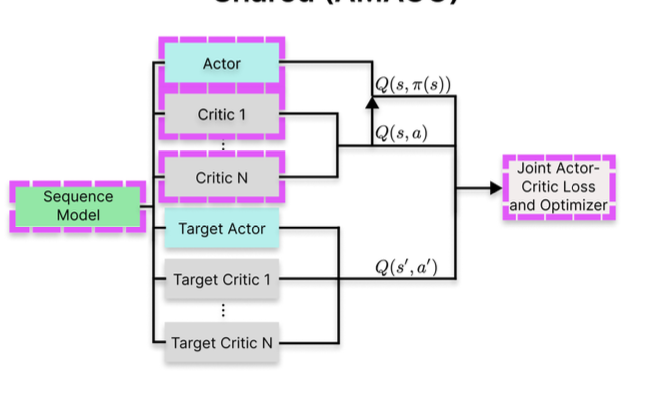
\includegraphics[height=1.5in]{figs/amago}
    \caption{
      The Amago actor-critic model.
      Purple boxes are involved in training.
      The green box is a the slow-to-train transformer backbone.
      The blue actor and gray critics are lightweight feedforward
      output heads.
\figtaken{Figure 10 if \citep{Grigsby2024}}.
}
\label{fig:amago}
\end{figure}

The recent  \keywordDef{Amago} algorithm \citep{Grigsby2024}
modifies the discrete SAC algorithm by considering  $\alpha=0$;
they  end up with a learning rule similar to DDPG (\cref{sec:DDPQ}).
In more detail,
%let $\vq_s = [Q(s,a_1),\ldots,Q(s,a_K)]$ be a vector
%of $Q$ values for each possible action, and let
%$\vmu_s = [\pi(a_1|s), \ldots, \pi(a_K|s)]$ be a vector
%of action probabilities.
let $\overline{Q}$ and $\overline{\pi}$ represent the frozen
(target) values of these functions, derived from EMA.
The critic loss can be written as an average
of the following loss, where we sample tuples from the replay buffer:
\be
  \loss_{\text{TD}}(\vs,a,r,\vs') = (Q(\vs,a) - (r+\gamma
    \stopgrad(\overline{V}(\vs,a)))^2 
  \ee
where the  value function is given by
\begin{align}
  \overline{V}(\vs) &=
  \sum_a \overline{\pi}(a|\vs) \overline{Q}(\vs,a)
  \end{align}
The actor  loss
(which we want to minimize, so negative of the previous objective)
is given by an average of the following loss,
where we sample states from the replay buffer:
\begin{align}
  \loss_{\text{PG}}(\vs) &= -\sum_a    \pi(a|\vs) Q(\vs,a)
\end{align}

In the limit that the policy becomes deterministic,
the value function becomes
\be
\overline{V}(\vs,a) = \overline{Q}(\vs,\overline{\pi}(\vs))
\ee
which is plugged into the critic loss.
The actor loss becomes 
\begin{align}
  \loss_{\text{PG}}(\vs)=-Q(\vs, \pi(\vs))
\end{align}
This gives an update similar to DDPQ.
Note that exploration can be ensured by using
a method such as epsilon-greedy, even if the policy is deterministic.
%Furthermore, the policy network still learns a distribution,
%which can be sampled from.

The actor and critic are both defined in terms of a shared
transformer sequence model,
with different output heads. (In fact they  have $N$ output heads
for the different $Q$ functions, as in REDQ, and maintain
a target version of the policy and the $N$ critics,
as shown in \cref{fig:amago}.
To train the shared model, they 
 construct a unified objective
$\loss = E[\lambda_0 \loss_{TD} + \lambda_1 \loss_{PG}]$,
where the TD and policy gradient losses are dynamically normalized
using the \keywordDef{PopArt} method
of \citep{van-Hasselt2016,Hessel2019}
to allow
for a fixed set of hyper-parameter values for $\lambda_i$,
even as the range of the losses change over time.
%(PopArt  stands for
%``Preserving Outputs Precisely, while Adaptively Rescaling Targets''.)
They show good results on challenging environments such as MineCraft.

}

\eat{
  
Yes, the discrete version is implemented like SAC-Discrete, where the actor outputs a softmax over actions, and the critic uses that distribution to reduce variance. In my experience, the main benefit of SAC's entropy is that it smooths TD targets in the critic update (similar to the manual noise of TD3) rather than the exploration improvement it's usually motivated by. When another technique is already stabilizing the critic update, it reduces tuning to remove entropy constraints and ensure exploration with a more intuitive epsilon-greedy schedule.

AMAGO has a second actor term that does weighted max likelihood on actions from the buffer. This is the main reason we need the actor network for discrete environments rather than taking the argmax over the critic like DQN variants. It also makes the discrete and continuous versions very similar. The second loss term is a safety measure for when the critic is inaccurate, as it essentially reduces the update to supervised learning with a Transformer. This turns out to be more important for multi-task problems than we thought and we're about to release a follow-up paper about it.

The update has the same theoretical properties as DDPG in an MDP
because the policy is allowed to become deterministic if that turns
out to be optimal. In meta-RL/POMDPs we’d rather be able to learn a
stochastic policy when the model has finite memory length, and we
always sample during evaluation.
}







\section{Deterministic policy gradient methods}
\label{sec:DPG}

In this section, we consider the case of a deterministic
policy, that predicts a unique action for each state,
so $a_t = \policydet(s_t)$,
rather than $a_t \sim \polapprox(s_t)$.
(We require that the actions are continuous,
because we will take the Jacobian of the $Q$ function
wrt the actions; if the actions are discrete,
we can just use DQN.)
The advantage of using a deterministic policy
is that we can modify the policy gradient method
so that it can work off policy without
needing importance sampling, as we will see.


Following
\cref{eqn:JJpi},
we define the value of a policy as the expected discounted
reward per state:
\begin{align}
\polval(\policydet)
%= \int_S \statdistdet(s) R(s, \policydet(s)) ds
\defeq  \expectQ{R(s,\policydet(s))}{\statmeasuredet(s)}
\end{align}
The \keywordDef{deterministic policy gradient theorem}
\citep{dpg} tells us that the gradient of this expression
is given by
\begin{align}
\nabla_{\vtheta} \polval(\policydet)
&=  \expectQ{\nabla_{\vtheta} \Qdet(s,
  \policydet(s))}
      {\statmeasuredet(s)} \\
&= \expectQ{\nabla_{\vtheta} \policydet(s)
 \nabla_a \Qdet(s, a)|_{a=\policydet(s)}}{\statmeasuredet(s)}
\label{eqn:DDPGgrad}
\end{align}
where $\nabla_{\vtheta} \policydet(s)$ is
the $M \times N$ Jacobian matrix,
and $M$ and $N$ are the dimensions
of $\calA$ and $\vtheta$, respectively.
%the number of action dimensions,
%and $N$ is the number of policy parameters.
For stochastic policies of the form
$\polapprox(a|s) = \policydet(s) + \text{noise}$,
the standard policy gradient theorem reduces
to the above form as the noise level goes to zero.

Note that the gradient estimate
in \cref{eqn:DDPGgrad}
integrates over the states but not over the actions,
which helps reduce the variance in gradient estimation
from sampled trajectories.
However, since the deterministic policy does not do any exploration,
we need to use an \keyword{off-policy method} for training.
This collects data from 
a stochastic behavior policy $\behavior$,
whose stationary state distribution is
$\statdistbehave$.
%We define the objective in a similar way to \cref{eqn:offPolicyJ}:
The original objective, $\polval(\policydet)$, is approximated by the following:
\begin{align}
\polvalbeh(\policydet)
\defeq \expectQ{\Vdet(s)}{\statdistbehave(s)}
= \expectQ{\Qdet(s, \policydet(s))}{\statdistbehave(s)}
\end{align}
with the off-policy deterministic policy gradient
from \citep{Degris2012}
is approximated by
%(see also \cref{sec:offpolicyRL-IS})
\begin{align}
\label{eqn:OffDDPGgrad}
\nabla_{\vtheta} \polvalbeh(\policydet)
\approx \expectQ{\nabla_{\vtheta} \left[\Qdet(s,
    \policydet(s))\right]}
        {\statdistbehave(s)}
= \expectQ{\nabla_{\vtheta} \policydet(s)
 \nabla_a \Qdet(s, a)|_{a=\policydet(s)}  }{\statdistbehave(s)}
\end{align}
where we have a dropped a term that depends on
$\nabla_{\vtheta} \Qdet(s,a)$ and is hard to estimate
\citep{dpg}.

To apply \cref{eqn:OffDDPGgrad}, we may learn $\Qapprox \approx \Qdet$ with TD,
giving rise to the following updates:
\begin{align}
\delta &= r_t + \gamma \Qapprox(s_{t+1}, \policydet(s_{t+1}))
- \Qapprox(s_t, a_t) \\
\vw_{t+1} &\assign \vw_t + \lr_{\vw} \delta \nabla_{\vw} \Qapprox(s_t,a_t) \\
\vtheta_{t+1} &\assign \vtheta_t + \lr_{\vtheta} \nabla_{\vtheta} \policydet(s_t)
\nabla_a \Qapprox(s_t,a)|_{a=\policydet(s_t)} 
\end{align}
So we learn both a state-action critic $Q_{\vw}$
and an actor $\vmu_{\vtheta}$.
This method avoids importance sampling
in the actor update because
of the deterministic policy gradient,
and we avoids it  in the critic
update because of the use of Q-learning.

If $\Qapprox$ is linear in $\vw$, and uses features
of the form $\vphi(s,a) = \va^\trans \nabla_{\vtheta} \policydet(s)$,
%where $\va$ is the vector representation of $a$,
then we say the function approximator for the critic
is \keywordDef{compatible} with the actor;
in this case, one can show that the above approximation
does not bias the overall gradient.
%Of course, this is rather restrictive.

%https://www.reddit.com/r/reinforcementlearning/comments/fafi7j/actorcritic_for_discrete_action_space/

The basic off-policy
DPG method has been extended in various ways,
some of which we describe below.

\subsection{DDPG}
\label{sec:DDPG}
\label{sec:D4PG}


The \keywordDef{DDPG} algorithm of \citep{ddpg},
which stands for
``\keyword{deep deterministic policy gradient}'',
uses  the DQN method (\cref{sec:DQN})
to update $Q$ that is represented by deep neural networks.
%
In more detail, the actor tries to minimize the output of the critic
by optimize
\be
\loss_{\vtheta}(s) = Q_{\vw}(s, \mu_{\vtheta}(s))
\ee
averaged over states $s$ drawn from the replay buffer.
The  critic tries to minimize
the 1-step TD loss
\be
\loss_{\vw}(s,a,r,s') =
[Q_{\vw}(s,a) - (r + \gamma Q_{\overline{\vw}}(s',\mu_{\vtheta}(s')))]^2
\ee
where $Q_{\overline{\vw}}$ is the target critic network,
and the samples $(s,a,r,a')$ are drawn from a replay buffer.
(See \cref{sec:targetNetwork} for a discussion of target networks.)

The \keywordDef{D4PG} algorithm \citep{D4PG},
which stands for ``distributed distributional DDPG'',
extends DDPG to
handle distributed training,
and to handle \keyword{distributional RL}
(see \cref{sec:distributional}).


\subsection{Twin Delayed DDPG (TD3)}
\label{sec:TD3}

The  \keywordDef{TD3} (``twin delayed deep deterministic'') method of
\citep{TD3}
extends DDPG  in 3 main ways.
First, it uses \keywordDef{target policy smoothing},
in which noise is added to the action, to encourage generalization:
\be
\tilde{\va} = \vmu_{\vtheta}(\vs) + \text{noise}
= \pi_{\vtheta}(\vs)
\ee
Second it uses \keywordDef{clipped double Q learning},
which is an extension of the double Q-learning discussed in
\cref{sec:double} to avoid
over-estimation bias.
In particular, the target values for TD learning are defined using
\be
\TargetV(r,\vs'; \overline{\vw}_{1:2}, \overline{\vtheta})
= r + \gamma \min_{i=1,2}
Q_{\overline{\vw}_i}(\vs', \pi_{\overline{\vtheta}}(\vs'))
\ee
Third, it uses \keywordDef{delayed policy updates},
in which it only updates the policy after the value function
has stabilized. (See also \cref{sec:bilevel}.)
See \cref{algo:TD3} for the pseudcode.


\begin{algorithm}
\dontprintsemicolon
\caption{TD3}
\label{algo:TD3}
Initialize environment state $\vs$,
policy parameters $\vtheta$,
target policy parameters $\overline{\vtheta}$,
critic parameters $\vw_i$,
target critic parameters $\overline{\vw}_i = \vw_i$,
replay buffer $\data=\emptyset$,
discount factor $\gamma$,
EMA rate $\rho$,
step size $\lr_{\vw}$, $\lr_{\vtheta}$.
\\
\Repeat{converged}
       {
         $\va = \mu_{\vtheta}(\vs) + \text{noise}$ \\
         $(\vs',r) = \text{step}(\va, \vs)$ \\
         $\data := \data \union
         \{ (\vs, \va, r, \vs') \}$ \\
         $\vs \assign \vs'$ \\
         \For{$G$ updates}{
         Sample a minibatch $\calB = \{(\vs_j,\va_j,r_j,\vs'_j)\}$
         from $\data$ \\
           $\vw = \text{update-critics}(\vtheta, \vw, \calB)$
         }
         Sample a minibatch $\calB = \{(\vs_j,\va_j,r_j,\vs'_j)\}$
         from $\data$\\
         $\vtheta = \text{update-policy}(\vtheta,\vw, \calB)$
        }
.\\
$\text{def update-critics}(\vtheta,\vw,\calB)$: \\
       Let $(\vs_j,\va_j,r_j,\vs'_j)_{j=1}^B = \calB$ \\
       \For{$j=1:B$}{
         $\tilde{\va}_j = \mu_{\overline{\vtheta}}(\vs'_j)
         + \text{clip}(\text{noise}, -c, c)$ \\
         $\targetV_j = r_j + \gamma \min_{i=1,2} Q_{\overline{\vw}_i}(\vs'_j,
         \tilde{\va}_j)$
       }
       \For{$i=1:2$}
    {
      $\loss(\vw_i) = \frac{1}{|\calB|} \sum_{(\vs,\va,r,\vs')_j \in
        \calB} (Q_{\vw_i}(\vs_j,\va_j) - \stopgrad(\targetV_j))^2$\\
      $\vw_i \assign \vw_i - \lr_{\vw} \nabla \loss(\vw_i)$ // Descent
      \\
      $\overline{\vw}_i := \rho \overline{\vw}_i
      + (1-\rho) \vw_i$       //Update target networks with EMA\\
    }

    Return $\vw_{1:N}, \overline{\vw}_{1:N}$\\
.\\
$\text{def update-actor}(\vtheta,\vw,\calB)$: \\
$J(\vtheta) =
 \frac{1}{|\calB|} \sum_{\vs \in \calB}
 \left(Q_{\vw_1}(\vs, \mu_{\vtheta}(\vs)) \right)^2$ \\
 $\vtheta \assign \vtheta +  \lr_{\vtheta} \nabla J(\vtheta)$ //
 Ascent \\
       $\overline{\vtheta} := \rho \overline{\vtheta}
       + (1-\rho) \vtheta$       //Update target policy network with EMA \\
         Return $\vtheta, \overline{\vtheta}$
\end{algorithm}






\eat{
\section{Gradient-free methods}
\label{sec:PGrnd}

The policy gradient
estimator computes a ``zeroth order'' gradient, which essentially
evaluates the function with randomly sampled trajectories.
Sometimes it can be more efficient to
use a derivative-free optimizer (\cref{sec:DFO}),
that does not even attempt to estimate the gradient.
For example, \citep{Mania2018} obtain good results
by training linear policies with random search,
and \citep{Salimans2017ES} show how to use
evolutionary strategies to optimize the policy
of a robotic controller.
}

%\chapter{Model-based RL}
\label{sec:MBRL}

% https://jonathan-hui.medium.com/rl-model-based-reinforcement-learning-3c2b6f0aa323

Model-free approaches to RL typically
need a lot of interactions with the environment
to achieve good performance.
For example, state of the art
methods for the Atari benchmark, such as \keyword{rainbow}
(\cref{sec:DQN}), use millions of frames,
equivalent to many days of playing
at the standard frame rate.
By contrast, humans can achieve the same
performance in minutes \citep{Tsividis2017}.
Similarly,
OpenAI's robot hand controller \citep{Andrychowicz2020}
needs  100 years of simulated data
to 
learn to manipulate a rubiks cube.


One promising approach to greater sample efficiency
is \keywordDef{model-based RL}
(\keywordDef{MBRL}).
In the simplest approach to MBRL,
we first learn the state transition or dynamics model
$\ptran(s'|s,a)$ --- also called a \keywordDef{world model} ---
and the reward function $R(s,a)$,
using some offline trajectory data, 
and then we use these models to compute a  policy
(e.g., using dynamic programming, as discussed in
\cref{sec:rl-planning},
or using some model-free policy learning method on simulated data,
as discussed in \cref{sec:policySearch}).
It can be shown that the sample complexity
of learning the dynamics is less than the sample
complexity of learning the policy \citep{Zhu2024iclr}.

However, the above two-stage approach --- where we first learn the model,
and then plan with it --- can suffer from the usual problems
encountered in offline RL (\cref{sec:offlineRL}),
i.e., the policy may query the model at a state
for which no data has been collected, so predictions can be
unreliable, causing the policy to learn the wrong thing.
To get better results, we have to interleave the model learning
and policy learning, so that one helps the other
(since the policy determines what data is collected).
%We discuss this in \cref{sec:MBRLgame}.
%However, we start in \cref{sec:MPC} by discussing the RL
%problem in the case where the model is known.

There are two main ways to perform MBRL.
In the first approach,
known as  \keywordDef{decision-time planning}
or \keywordDef{model predictive control},
we use the model
to choose the next action by searching over possible future
trajectories.
We then score each trajectory, pick the action corresponding to the best one, take
a step in the environment, and repeat.
(We can also optionally update the model
based on the  rollouts.)
This is discussed in \cref{sec:rollout}.

The second approach is to use the current model and policy
to rollout imaginary trajectories,
and to use this data
(optionally in addition to empirical data)
to  improve the policy using model-free RL;
this is called \keywordDef{background planning},
and is discussed in \cref{sec:backgroundPlanning}.


The advantage of decision-time planning is that
it  allows us to train a world model on reward-free data,
and then use that model
to optimize any reward function.
This can be particularly useful if the reward
contains changing constraints,
or if it is  an intrinsic reward (\cref{sec:intrinsic})
that frequently changes based on the knowledge state of the agent.
The downside of decision-time planning is that it is much slower.
However, it is possible to combine the two methods, as we discuss below.
For an empirical comparison of
background planning and decision-time planning,
see  \citep{Alver2024background}.

Some generic pseudo-code for an MBRL agent is given
in \cref{algo:MBRL}.
(The {\tt rollout} function is defined in \cref{algo:rollout};
some simple  code for model learning is
shown in \cref{algo:update-model},
although we discuss other loss functions in  \cref{sec:WM};
%the code for the sampling functions is omitted, since it is trivial;
finally, the code for the policy learning is given in other parts of this manuscript.)
For more details on general MBRL, see
e.g., \citep{Wang2019MBRL,Moerland2023,Plaat2021}.



\begin{algorithm}
\dontprintsemicolon
\caption{MBRL agent}
\label{algo:MBRL}
def MBRL-agent$(\Mtrue; T, H, N)$: \\
Initialize state $s \sim \Mtrue$ \\
Initialize data buffer $\data=\emptyset$, model $\hat{M}$ \\
Initialize value function $V$, policy proposal $\pi$\\
\Repeat{until converged}
       {
       // Collect data from environment \\
         $\tau_{\tenv} = \text{rollout}(s, \pi, T, \Mtrue)$, \;
      $s = \tau_{\tenv}[-1]$, \;
      $\data = \data \union \tau_{\tenv}$ \\
      // Update model \\
         \If{Update model online}
            {
        $\hat{M} = \text{update-model}(\hat{M}, \tau_{\tenv})$\\
              }
              \If{Update model using replay}
              {
                %$\tau_{\treplay}^{1:N} =\text{sample-traj-from-replay}(\data, N)$ \\
                $\tau_{\treplay}^{n} =\text{sample-trajectory}(\data), n=1:N$ \\
                $\hat{M} = \text{update-model}(\hat{M}, \tau_{\treplay}^{1:N})$\\
              }

   // Update policy \\
          \If{Update on-policy with real}
                 {
                   $(\pi,V)=\text{update-on-policy}(\pi,V,\tau_{\tenv})$\\
                 }
           \If{Update on-policy with imagination}
                    {
                      %$\tau_{\timag}^{1:N}=\text{sample-traj-from-model}(\data,\hat{M},\pi,T,N)$ \\
                      $\tau_{\timag}^{n}=\text{rollout}(\text{sample-init-state}(\data),\pi,T,\hat{M}), n=1:N$ \\
           $(\pi,V)=\text{update-on-policy}(\pi,V,\tau_{\timag}^{1:N})$ 
           }

          \If{Update off-policy with real}
           {
             %$\tau_{\treplay}^{1:N}=\text{sample-traj-from-replay}(\data,N)$ \\
             $\tau_{\treplay}^{n} =\text{sample-trajectory}(\data), n=1:N$ \\
             $(\pi,V)=\text{update-off-policy}(\pi,V,\tau_{\treplay}^{1:N})$\\
           }
           \If{Update off-policy with imagination}
           {
             %$\tau_{\timag}^{1:N}=\text{sample-traj-from-model}(\data,\hat{M},\pi,T,N)$ \\
             $\tau_{\timag}^{n}=\text{rollout}(\text{sample-state}(\data),\pi,T,\hat{M}), n=1:N$ \\
              $(\pi,V)=\text{update-off-policy}(\pi,V,\tau_{\timag}^{1:N})$\\
            }

}
\end{algorithm}



\begin{algorithm}
\dontprintsemicolon
\caption{Rollout}
\label{algo:rollout}
def rollout$(s_1, \pi, T, M)$ \\
$\tau=[s_1]$ \\
\For{$t=1:T$}{
  $a_t = \pi(s_t)$ \\
  $(s_{t+1}, r_{t+1}) \sim M(s_t,a_t)$ \\
  $\tau += [a_t, r_{t+1}, s_{t+1}]$
  }
Return $\tau$ 
\end{algorithm}


\begin{algorithm}
\dontprintsemicolon
\caption{Model learning}
\label{algo:update-model}
 def update-model$(M,\tau^{1:N}):$\\
 $\lossfn(M) = -\frac{1}{N T}\sum_{n=1}^N \sum_{(s_t,a_t,r_{t+1},s_{t+1}) \in \tau^n}
 \log M(s_{t+1},r_{t+1}| s_t,a_t)$ // NLL \\
    $M = M - \lr_M \nabla_M \lossfn(M)$ \\
    Return $M$\\
\end{algorithm}


\section{Decision-time planning}
\label{sec:rollout}
\label{sec:decisionTimePlanning}

If the model is known, and the state and action space is discrete
and low dimensional,
we can use exact techniques
based on dynamic programming to compute the policy,
as discussed in \cref{sec:planning}.
However, for the general case,
approximate  methods must be used for planning,
whether the model is known (e.g., for board games like Chess and Go)
or learned.

One approach to approximate planning
is to be lazy, and 
just  wait until we know what state we are in,
call it $s_t$, and then decide what to do,
rather than trying to learn a policy that maps any state to the best action.
This is called \keywordDef{decision time planning}
or  ``\keywordDef{planning in the now}''
\citep{Kaelbling2011}.
We discuss some variants of this approach below.

\subsection{Model predictive control (MPC)}
\label{sec:MPC}

We now describe a method
 known as \keywordDef{receeding horizon control}
or \keywordDef{model predictive control} (\keywordDef{MPC})
\citep{Mayne1990,Camacho2013,Rawlings2022}:
We use the world model to predict future states and rewards that might  follow
from the current state
for each possible sequence of future actions we might pursue,
and we then take the action from the sequence that looks most promising.
More precisely, at each step, we compute
\begin{align}
  \va_{t:t+H-1}^* &=  \text{planning}(s_t, M, R, \hat{V}, H) \\
  &= \argmax_{\va_{t:t+H-1}}
\expectQ{\sum_{h=0}^{H-1} R(s_{t+h}, a_{t+h}) + \hat{V}(s_{t+H})}
{s_{t+1:t+H} \sim M(\cdot|s_t, a_{t:t+H-1})} 
\label{eqn:MPC} \\
\pi_{\tmpc}(s_t) &= a_t^*
\end{align}
%where the expectation is over state sequences that
%might result from executing $\va_{t:t+H-1}$ from state $s_t$.
Here, $H$ is called the \keywordDef{planning horizon},
and $\hat{V}(s_{t+H})$ is an estimate of the reward-to-go
at the end of this $H$-step look-ahead process.
We can often speed up the optimization process
by using a pre-trained proposal policy $a_t=\pi(s_t)$,
which can be used to guide the search process, as we discuss below.

Note that MPC computes a fixed sequence of actions, $\va_{t:t+H-1}$,
also called a plan,  given the current state $\vs_t$;
since the future actions $\va_{t'}$ for $t'>t$
are independent of the future states $\vs_{t'}$,
this is called an \keywordDef{open loop controller}.
Such a controller can work well in deterministic environments
(where $\vs_{t'}$ can be computed from $\vs_t$ and the action sequence),
but in general, we will need to replan at each step,
as the actual next state is observed.
Thus MPC is a way of creating
a \keywordDef{closed loop controller}.


We can combine MPC with model and policy/proposal learning
using the  pseudocode in \cref{algo:MBRL},
where the decision policy $a_t = \pi_{\tmpc}(s_t)$ is implemented
by \cref{eqn:MPC}.
If we want to learn the propsoal policy
$a_t=\pi(s_t)$, we should use off-policy methods,
since the training data (even if imaginary)
will be collected by $\pi_{\tmpc}$
rather than by $\pi$.
When learning the world model,
we only need it to be
locally accurate, around the current state,
which means we can often use simpler models in MPC
than in background planning approaches.

In the sections below, we discuss particular kinds of MPC methods.
Further connections between MPC and RL
are discussed in \citep{Bertsekas2024MPC}.


\subsection{Heuristic search}
\label{sec:heuristicSearch}
\label{sec:heuristic}
\label{sec:Astar}

\begin{figure}
\centering
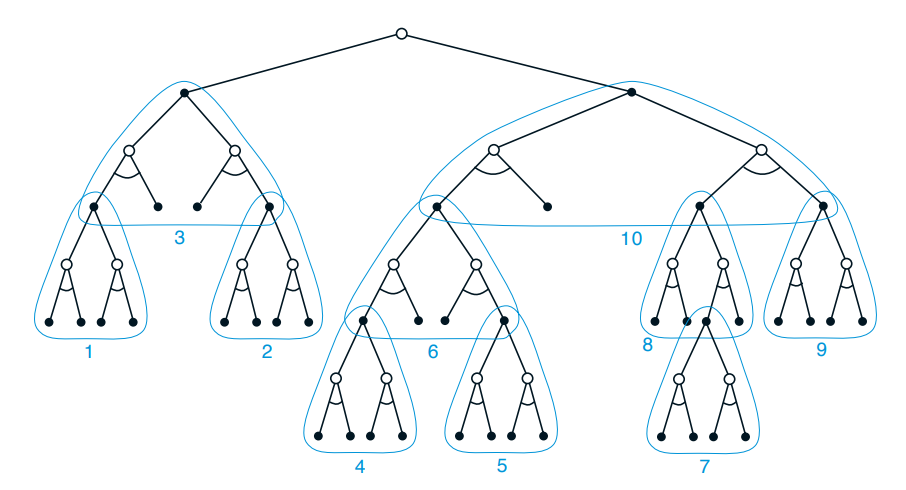
\includegraphics[height=1.5in]{figs/sutton-8-9}
\caption{
  Illustration of  heuristic search.
  In this figure,
  the subtrees
  are ordered  according to a depth-first search
  procedure.
  \figtaken{Figure 8.9 of \citep{Suttonv2}}.
\figthanks{Richard Sutton}.
}
\label{fig:sutton-8-9}
\end{figure}

If the state and action spaces are finite,
we can solve \cref{eqn:MPC}  exactly,
although the time complexity will typically
be exponential in $H$.
However, in many situations,
we can prune off unpromising trajectories,
thus making the approach feasible in large scale problems.

In particular, consider
a discrete, deterministic MDP
where reward maximization corresponds to finding
a shortest path to a goal state.
We can expand the successors of the current state
according to all possible actions, trying to find the goal state.
Since the search tree grows exponentially with depth,
we can use a \keywordDef{heuristic function} to prioritize
which nodes to expand;
this is called \keywordDef{best-first search},
as illustrated in \cref{fig:sutton-8-9}.

If the heuristic function is an optimistic lower bound
on the true distance to the goal, it is called
\keywordDef{admissible}.
If we aim to maximize total rewards,
admissibility means the heuristic function is
an upper bound of the true value function.
Admissibility ensures we will never
incorrectly prune off parts of the search space.
In this case, the resulting algorithm is known
as \keywordSpecial{$A^*$ search}{A* search},
and is optimal.
%
For more details on classical AI
\keywordDef{heuristic search} methods,
see \citep{Pearl1984,aima}.


\eat{
In the AI literature, the heuristic function
(which approximates the value function for the MDP)
is usually manually
designed. However, we can use RL methods to learn
the value function, as we discuss in \cref{sec:valueBased}.
For example, \keywordDef{TD-Gammon} \citep{Tesauro95}
uses temporal difference learning (\cref{sec:TD})
to learn a value function for the game of backgammon,
using a form of heuristic search to pick actions at each step.
(The world model $p(s'|s,a)$ was based on the statistics
of dice rolls, combined with the assumption that the opposing
player would act optimally according to TD-gammon's current model.)
}





\subsection{Monte Carlo tree search}
\label{sec:MCTS}





\keywordDef{Monte Carlo tree search}
or \keywordDef{MCTS} is similar to heuristic search,
but learns a value function for each encountered state,
rather than relying on a manually designed heuristic
(see e.g., \citep{Munos2014} for details).
MCTS is inspired by the upper confidence bound (UCB)
method for bandits,
but works for general MDPs \citep{Kocsis06}.

\subsubsection{AlphaGo and AlphaZero}
\label{sec:alphaGo}
\label{sec:alphaZero}

% Sutton p448
The famous \keywordDef{AlphaGo} system \citep{alphaGo},
which was the first AI system to beat a human grandmaster at the board game Go,
used the MCTS method,
combined with a value function learned using RL,
and a policy that was initialized using supervised learning
from human demonstrations.
This was followed up by \keywordDef{AlphaGoZero}
\citep{alphaGoZero},
which had a much simpler design,
and did not train on any human data,
i.e., it was trained entirely using RL and self play.
It significantly outperformed the original AlphaGo.
This was generalized to \keywordDef{AlphaZero} 
\citep{alphaZero},
which can play expert-level Go, chess, and shogi (Japanese chess),
using a known model of the environment.
%In \cref{sec:muZero}, we discuss how to extend AlphaZero
%to the case where the world model must be learned.





\subsubsection{MuZero}
\label{sec:muZero}

AlphaZero  assumes the world model is known.
The \keywordDef{MuZero} method of 
\citep{Schrittwieser2020}
learns a world model, by training a latent
representation of the observations, $\vz_t=\phi(\vo_t)$,
and a corresponding latent dynamics model $\vz_t=M(\vz_t,a_t)$.
The world model is trained
to predict the immediate reward,
the future reward (i..e, the value),
and the optimal policy,
where the optimal policy is computed 
using MCTS.

\newcommand{\mcts}{\text{MCTS}}

In more detail,
to learn the model, MuZero uses a sum of 3 loss terms
applied to each $(\vz_{t-1}, a_{t}, \vz_{t}, r_{t})$
tuple in the replay buffer.
The first loss is
$\loss(r_t, \hat{r}_t)$, where $r_t$ is the observed reward
and $\hat{r}_t=R(\vz_{t})$ is the predicted reward.
The second loss is
$\loss(\vpi^{\mcts}_t, \vpi_t)$, where $\vpi^{\mcts}_t$ is the target policy
from MCTS search (see below)
and $\vpi_t = f(\vz_t)$ is the predicted policy.
The third loss is
$\loss(G_t^{\mcts}, v_t)$,
where  $G^{\mcts}_t = \sum_{i=0}^{n-1} \gamma^i r_{t+i} + \gamma^k v_{t+n}$
is the n-step bootstrap
target value derived from MCTS search (see below),
and $v_t=V(\vz_t)$ is the predicted value from the current model.


To pick an action, MuZero does not use the policy directly.
Instead it uses MCTS to rollout a search tree
using the dynamics model, starting from the current state $\vz_t$.
It uses the predicted policy  $\vpi_t$ and value $v_t$
as heuristics to limit the breadth and depth of the search.
Each time it expands a node in the tree, it assigns it a unique
integer id (since we are assuming the dynamics are deterministic),
thus lazily creating a discrete MDP.
It then partially solves for the tabular $Q$ function for this MDP
using Monte Carlo rollouts,
similar to real-time dynamic programming (\cref{sec:RTDP}).

In more detail, the MCTS process is as follows.
Let $s^k=\vz_t$ be the root node, for $k=0$.
We initialize $Q(s^k,a)=0$ and $P(s^k,a)=\vpi_t(a|s^k)$,
where the latter is the prior for each action.
To select the action $a^k$ to perform next (in the rollout),
we  use the UCB heuristic  (\cref{sec:UCB})
based on the empirical counts $N(s,a)$
combined with  the prior policy, $P(s,a)$,
which act as pseudocounts.
After expanding this node, we  create the child node
$s^{k+1}=M(s^k,a^k)$;
we initialize $Q(s^{k+1},a)=0$ and $P(s^{k+1},a)=\vpi_t(a|s^{k+1})$,
and repeat the process until we reach a maximum depth,
where
we apply the value function to the corresponding leaf node.
We then compute the empirical sum of discounted rewards along each of the
explored paths, and use this to update the $Q(s,a)$ and $N(s,a)$
values for all visited nodes.
After performing 50 such rollouts, we compute the empirical
distribution
over actions at the root node to get the MCTS visit count policy,
$\vpi^{\mcts}_t(a) = [N(s^0,a)/(\sum_b N(s^0,b))]^{1/\tau}$,
where $\tau$ is a temperature.
Finally we sample an action $a_{t}$ from $\vpi^{\mcts}_t$,
take a step,
add $(o_t, a_t, r_t, \vpi_t^{\mcts}, G_t^{\mcts})$ to the replay buffer,
compute the losses, update the model and policy parameters, and repeat.


The  \keywordDef{Stochastic MuZero} method
of \citep{Antonoglou2022} extends MuZero to allow for stochastic
environments.
The \keywordDef{Sampled MuZero} method of \citep{Hubert2021}
extends MuZero to allow for large action spaces.



\subsubsection{EfficientZero}
\label{sec:efficientZero}


The \keywordDef{Efficient Zero}
paper  \citep{efficientZero} extends MuZero by adding
an additional  self-prediction loss to help train the world model.
(See \cref{sec:SPR} for a discussion of such losses.)
It also makes several other changes.
In particular, it replaces the empirical sum of instantaneous rewards,
$\sum_{i=0}^{n-1} \gamma^i r_{t+i}$,
used in computing $G_t^{\mcts}$,
with an LSTM model that predicts the sum of rewards
for a trajectory starting at $\vz_t$;
they call this the value prefix.
In addition, 
it replaces the stored value at the leaf nodes
of trajectories in the replay buffer with new values,
by rerunning MCTS using the current model
applied to  the leaves.
They show that all three changes help,
but the biggest gain is from the self-prediction  loss.
The recent \keywordDef{Efficient Zero V2}
\citep{efficientZeroV2} extends this to also work with continuous
actions,
by replacing tree search with sampling-based Gumbel search,
amongst other changes.



\subsection{Trajectory optimization for continuous actions}



For continuous actions, we cannot enumerate
all possible branches in the search tree.
Instead, we can view \cref{eqn:MPC}
as a standard optimization problem over
the real valued sequence of vectors $\va_{t:t+H-1}$.

\subsubsection{Random shooting}

For general nonlinear models (such as neural networks),
a simple approach
is to pick a sequence of random actions to try,
evaluate the reward for each trajectory,
and pick the best.
This is called \keywordDef{random shooting}
\citep{Diehl2007,Rao2010}.

\subsubsection{LQG}

If the system dynamics are linear
and the reward function corresponds to
negative quadratic cost,
the optimal action sequence can be solved
mathematically, as in the
\keywordDef{linear-quadratic-Gaussian}
(\keywordDef{LQG}) controller
(see e.g., \citep{Anderson89,Hoffmann2017control}).

If the model is nonlinear, we can use
\keywordDef{differential dynamic programming}
(\keywordDef{DDP})~\citep{Jacobson70,Todorov05}.
In each iteration, DDP starts with a reference trajectory,
and linearizes the system dynamics around states on
the trajectory to form a locally quadratic approximation
of the reward function.
This system can be solved using LQG,
whose optimal solution results in a new trajectory.
The algorithm then moves to the next iteration,
with the new trajectory as the reference trajectory.



\subsubsection{CEM}
\label{sec:TDMPC}
\label{sec:CEM}


It common to use
black-box (gradient-free) optimization methods
like the \keywordDef{cross-entropy method} or \keywordDef{CEM}
in order to find the best action sequence.
The CEM method is a simple derivative-free optimization
method for continuous black-box functions $f: \real^D \ra \real$.
We start with a multivariate Gaussian, $\gauss(\vmu_0,\vSigma_0)$,
representing a distribution over possible action $\va$.
We sample from this, evaluate all the proposals,
pick the top $K$, then refit the Gaussian to these top $K$,
and repeat, until we find a sample with sufficiently good score
(or we perform moment matching on the top $K$ scores).
For details, see \citep{Rubinstein1997,Rubinstein2004,DeBoer2005}.

In \cref{sec:MPPI}, we discuss the MPPI method,
which is a common instantiation of CEM method.
Another example is
in the \keywordDef{TD-MPC} paper \citep{TDMPC}.
They learn the world model (dynamics model) in a latent space
so as to predict future value and reward using temporal difference learning,
and then use CEM to implement MPC for this world model.
%\citep{Pinneri2021} discusses ways to speedup CEM,
In \citep{Bharadhwaj2020} they discuss how to combine CEM with gradient-based planning.
\eat{
It is also possible to create differentiable versions
of CEM and to backpropagate through them
to train the dynamics model,
as we discuss in \cref{sec:differentiable-planning}.
}

\subsubsection{MPPI}
\label{sec:MPPI}

%such as \keywordDef{shooting} and
%\keywordDef{collocation}~\citep{Diehl2007,Rao2010,Kalakrishnan11}.
%Many of them work in an iterative fashion,
%starting with an initial action sequence
%followed by a step to improve it.
%This process repeats until convergence of
%the cost.

The \keywordDef{model predictive path integral}
or \keywordDef{MPPI} approach \citep{MPPI}
is a version of CEM. 
Originally MPPI was limited to models with linear dynamics,
but it was extended to general nonlinear models in 
\citep{Williams2017}.
The basic idea is that the initial mean of the Gaussian
at step $t$, namely $\vmu_t=\va_{t:t+H}$,
is computed based on shifting $\hat{\vmu}_{t-1}$ forward by one step.
(Here $\vmu_t$ is known as a reference trajectory.)

In \citep{Wagener2019}, they apply this method for robot control.
They consider a state vector
of the form $\vs_t=(\vq_t,\dot{\vq}_t)$, where $\vq_t$ is the
configuration
of the robot. The deterministic dynamics has the form
\be
\vs_{t+1} = F(\vs_t,\va_t) = \begin{pmatrix}
  \vq_t + \dot{\vq}_t \Delta t \\
  \dot{\vq}_t + f(\vs_t,\va_t) \Delta t
  \end{pmatrix}
\ee
where $f$ is a 2 layer MLP.
This is trained using the
\keywordDef{Dagger} method of \citep{Ross2011},
which alternates between fitting the model (using supervised learning)
on the current replay buffer (initialized with expert data),
and then deploying the model 
inside the MPPI framework to collect new data.


\subsubsection{GP-MPC}
\label{sec:GPMPC}

\citep{Kamthe2018}  proposed
\keywordDef{GP-MPC}, which combines a Gaussian process dynamics model
with model predictive control.
They  compute
a Gaussian approximation to the future state trajectory
given a candidate action trajectory,
$p(\vs_{t+1:t+H}|\va_{t:t+H-1},\vs_t)$,
by moment matching,
and use this to deterministically compute
the expected reward and its gradient wrt
$\va_{t:t+H-1}$.
%(as opposed to the policy parameters $\vtheta$).
Using this, they can solve \cref{eqn:MPC}
to find  $\va_{t:t+H-1}^*$;
finally, they execute the first step of this plan,
 $a_{t}^*$,
and repeat the whole process.


The key observation is that moment matching is a deterministic
operator that maps $p(\vs_t|\va_{1:t-1})$ to $p(\vs_{t+1}|\va_{1:t})$,
so the problem becomes one of deterministic optimal control,
for which many solution methods exist.
Indeed the whole approach can be seen as a generalization
of the \keywordDef{LQG} method from  classical control,
which assumes a (locally) linear dynamics model,
a quadratic cost function,
and a Gaussian distribution over states
\citep{Recht2019}.
In GP-MPC, the moment matching plays the role of local linearization.

The advantage of GP-MPC  over the earlier method
known as \keywordDef{PILCO}
(``probabilistic inference for learning control''),
which learns a policy  by maximizing the expected reward
from rollouts (see \citep{pilco,pilcoJ} for details),
is that GP-MPC can handle constraints more easily,
and it can be more data efficient,
since it continually updates the GP model after every  step
(instead of at the end of an trajectory).


\subsection{SMC for MPC}
\label{sec:SMCMPC}

A general way to tackle MPC --- which supports discrete and continuous actions,
as well as discrete and continuous states and linear and nonlinear world models ---
is to formulate it as the problem of
posterior inference over state-action sequences
with high reward.
That is, following the \keyword{control as inference} framework discussed in
\cref{sec:inferRL},
we define the goal as computing
the following posterior:
\be
p(\vx_{1:T} | \vs_1, O_{1:T})
\propto
p(\vx_{1:T},  O_{1:T} | \vs_1)
= 
\prod_{t=1}^{T-1} p(\vs_{t+1}|\va_t,\vs_t)
\exp\left( \sum_{t=1}^T R(\vs_t,\va_t)  + \log p(\va_t)
\right)
\ee
where $\vx_t=(\vs_t,\va_t)$,
and $O_t$ is the ``optimality variable''
which is clamped to the value 1,
with distribution
$p(O_t=1|\vs_t,\va_t) = \exp(R(s_t,a_t))$.
(Henceforth we will assume a uniform prior over actions,
so $p(\va_t) \propto 1$.)
If we can sample from this distribution,
we can find state-action sequences with high expected
reward, and then we can just extract
the first action from one of these sampled
trajectories.\footnote{
%
We should really marginalize over the state sequences,
and then find the maximum marginal probability action sequence,
as in \cref{eqn:MPC}, but we approximate
this by joint sampling, for simplicity.
For more discussion on this point, see \citep{Lazaro-Gredilla2024}.
}


In practice we  only compute the posterior
for $h$ steps into the future,
although we still condition on optimality
out to the full horizon $T$.
Thus we define our goal as computing
\be
p(\vx_{1:h} | O_{1:T})
\propto
\underbrace{p(\vx_{1:h} | O_{1:h})}_{\alpha_h(\vx_{1:h})}
\underbrace{p(O_{h+1:T}|\vx_h)}_{\beta_h(\vx_h)}
\label{eqn:target}
\ee
where $p(O_t=1|s_t,a_t) = \exp(R(s_t,a_t))$
is the probability that the ``optimality variable''
obtains its observed (clamped) value of 1.
We have decomposed the posterior as a forwards filtering term,
$\alpha_h(\vx_{1:h})$,
and a backwards likelihood or smoothing term,
$\beta_h(\vx_h)$,
as is standard in the literature
on inference in state-space models
(see e.g., \citep[Ch.8-9]{book2}).
Note that if we define the value function as
$V(\vs_h) = \log p(O_{h:T}|\vs_h)$,
then 
the backwards message can be rewritten as
follows  \citep{Piche2019}:
\be
p(O_{h+1:T}|\vx_h) = \expectQ{\exp(V(\vs_{h+1}))}{p(\vs_{h+1}|\vx_h)}
\ee

A standard way to perform posterior inference in 
models such as these is to use
 \keywordDef{Sequential Monte Carlo}
 or \keywordDef{SMC},
 which is an extension of particle filtering
 (i.e., sequential importance sampling with resampling)
 to a general sequence of distributions over a growing state space
 (see e.g., \citep[Ch 13.]{book2}).
 When combined with an approximation to the backwards message,
 the approach is called \keywordDef{twisted SMC}
\citep{Briers10,Whiteley2014,Ala-Luhtala2016,SIXO,Zhao2024}.
This was applied to MPC 
in  \citep{Piche2019}.
In particular, they suggest using SAC to learn a value function
$V$, analogous to the backwards twist function, and policy $\pi$,
which can be used to create the forwards proposal.
More precisely,
the policy can be combined with the world model
$M(\vs_t|\vs_{t-1},\va_{t-1})$ to give a (Markovian) proposal
disribution over the next state and action:
\be
q(\vx_t|\vx_{1:t-1}) = M(\vs_t|\vs_{t-1},\va_{t-1})
 \pi(\va_t|\vs_t)
 \ee
This can then be used inside of an SMC
algorithm to sample trajectories from  the posterior
in \cref{eqn:target}.
In particular, at each step, 
we sample from
the proposal to extend each 
previous particle (sampled trajectory) by one step,
and then reweight the corresponding particle using
\begin{align}
  w_t &= \frac{p(\vx_{1:T}|O_{1:T})}{q(\vx_{1:t})} 
    = \frac{p(\vx_{1:t-1}|O_{1:T}) p(\vx_t|\vx_{1:t-1},O_{1:T})}
      {q(\vx_{1:t-1}) q(\vx_t|\vx_{1:t-1})} \\
  &=  w_{t-1} \frac{p(\vx_t|\vx_{1:t-1},O_{1:T})}
  {q(\vx_t|\vx_{1:t-1})} 
  \propto  w_{t-1} \frac{1}{ q(\vx_t|\vx_{1:t-1})}
  \frac{ p(\vx_{1:t}|O_{1:T})}{p(\vx_{1:t-1}|O_{1:T})}
\end{align}
Now plugging in the forward-backward equation
from \cref{eqn:target}, and doing some algebra, we get
the following
(see  \citep[App. A.4]{Piche2019} for the detailed derivation):
\begin{align}
  w_t
  &\propto  w_{t-1} \frac{1}{ q(\vx_t|\vx_{1:t-1})}
 \frac{ p(\vx_{1:t}|O_{1:t}) p(O_{t+1:T}|\vx_t)}
      {p(\vx_{1:t-1}|O_{1:t-1}) p(O_{t:T}|\vx_{t-1})} \\
      &\propto  w_{t-1} \expectQ{
        \exp(A(\vs_t,\va_t,\vs_{t+1}))}{p(\vs_{t+1}|\vs_t,a_t)} 
\end{align}
where
\be
A(\vs_t,\va_t,\vs_{t+1})
= r_t - \log \pi(\va_t|\vs_t) + V(\vs_{t+1})
- \expectQ{\exp(V(\vs_t))}{p(\vs_t|\vs_{t-1},\va_{t-1})}
\ee
is a maximum entropy version of an advantage function.
We show the overall pseudocode in
\cref{algo:SMCMPC}.


\begin{algorithm}
\dontprintsemicolon
\caption{SMC for MPC}
\label{algo:SMCMPC}
def SMC-MPC($\vs_t, M, \pi,  V, H)$ \\
Initialize particles:  $\{\vs_t^n=\vs_t\}_{n=1}^N$ \\
Initialize weights: $\{w_t^n = 1\}_{n=1}^N$ \\
\For{$i=t:t+H$}
    {
      // Propose one-step extension \\
      $\{ \va_i^n \sim \pi(\cdot|\vs_i^n) \}$ \\
      $\{ (\vs_{i+1}^n, r_i^n) \sim M(\cdot | \vs_i^n, \va_i^n) \}$ \\
      // Update weights \\
      $\{ w_i^n \propto w_{i-1}^n \exp(A(\vs_i^n, \va_i^n, \vs_{i+1}^n)) \}$ \\
    // Resampling \\
    $\{ \vx_{1:i}^n \} \sim \text{Multinom}(n; w_i^1, \ldots, w_i^N)$ \\
    $\{ w_i^n = 1 \}$
    }
    Sample $n \sim \text{Unif}(1:N)$ // Pick one of the top samples \\
    Return $\va_t^n$ \\
%    Return $(\vs_{t:t+h}^n, \va_{t:t+h}^n)$ \\
\end{algorithm}


An improved version of the above method, called \keywordDef{Critic SMC},
is presented in \citep{Lioutas2022}.
The main difference is that  they first extend each of the $N$ particles
(sampled trajectories) by $K$ possible ``putative actions'' $a_i^{nk}$,
then score
them using a learned heuristic function $Q(s_i^n,a_i^{nk})$,
then resample $N$
winners $a_i^n$ from this set of $N \times K$ particles,
and then push these winners through the
dynamics model to get $s_{i+1}^n \sim M(\cdot|s_i^n,a_i^n)$.
Finally, they  reweight the $N$
particles by the advantage and resample, as before.
This can be advantageous  if the dynamics model is slow to evaluate,
since we can evaluate $K$ possible extensions just using the heuristic
function.
We can think of this as a form of stochastic beam search, where the beam
has $N$ candidates, and you expand each one using $K$ possible actions,
and then reduce the population  (beam) back to $N$



\eat{
\subsection{Amortized MPC}

MPC can be slow, since it requires rolling out the world model
for each candidate action sequence.
However, we can use the output of MPC as training data
for learning a reactive policy,
which can be trained with MLE (i.e., behavior cloning,
c.f., \cref{sec:BC}).
The above approach is a valid policy improvement operator,
as pointed out in the MuZero paper \citep{Schrittwieser2020}.
This follows from the policy improvement theorem
(\cref{sec:policyImprovement}):
we just set the new policy to be $\pi'(s) =a^* \neq \pi(s)$,
where $a^*$ is the result of lookahead search, and $\pi'$ is otherwise
the same as $\pi$.\footnote{
%
This policy improvement argument assumes a nonparametric (e.g., tabular) policy.
For a parametric model, updating $\pi'(s)$ to predict $a^*$ may also
affect the prediction for other states.
Furthermore,
this is only an improvement of the policy wrt the current world
model. If the model is wrong, it can also be incrementally updated,
usually using maximum
likelihood training on observed trajectories.
Methods to ensure both steps monotonically improve performance
are discussed in \cref{sec:MBRLrobust}.
}
We call this approach ``\keywordDef{amortized MPC}'',
since it amortizes the cost of doing MPC
by distilling the lookahead search process into
a model-free reactive policy.
}


\section{Background planning}
%\section{Jointly learning the model and policy}
\label{sec:MBRLcombine}
\label{sec:MBRLrobust}
\label{sec:backgroundPlanning}

In \cref{sec:decisionTimePlanning},
 we discussed how to use
models to perform decision time planning.
However, this can be slow.
Fortunately, we can amortize the planning process into a reactive
policy.
To do this, we can use the model to generate synthetic trajectories
``in the background'' (while executing the current policy),
and use this imaginary  data
to train the policy;
this is called ``\keywordDef{background planning}''.
We discuss a game theoretic formulation of this setup in
\cref{sec:MBRLgame}.
Then in \cref{sec:dyna},
we discuss ways to combine model-based and model-free learning.
Finally, in \cref{sec:modelUncertainty},
we discuss ways to deal with model errors, that might lead the policy astray.




\subsection{A game-theoretic perspective on MBRL}
\label{sec:MBRLgame}


In this section, we discuss a game-theoretic framework for 
MBRL, as proposed in  \citep{Rajeswaran2020}. This provides a theoretical
foundation for many of the more heuristic methods in the literature.

We denote the true world model  by $\Mtrue$.
To simplify the notation, we assume an MDP setup with a known 
reward function,
so all that needs to be learned is the world model, $\Mest$, representing
$p(s'|s,a)$.
(It is trivial to also learn the reward function.)
We define the value of a policy $\pi$ when rolled out in some model $M'$
as the (discounted) sum of expected rewards:
\begin{align*}
J(\pi,M') = \expectQ{\sum_{t=0}^{\infty} \gamma^t R(s_t)}{M',\pi}
\end{align*}
We define the loss of a model $\Mest$ given a distribution
$\mu(s,a)$ over states and actions as
\begin{align*}
  \lossfn(\Mest,\mu) = \expectQ{\KLpq{\Mtrue(\cdot|s,a)}{\Mest(\cdot|s,a)}}
  {(s,a) \sim \mu}
\end{align*}
We now define MBRL as a two-player general-sum game:
\begin{align*}
  \overbrace{\max_{\pi} J(\pi, \Mest)}^{\text{policy player}},
  \overbrace{\min_{\Mest} \lossfn(\Mest, \mu_{\Mtrue}^{\pi})}^{\text{model player}}
\end{align*}
where $\mu_{\Mtrue}^{\pi} = \frac{1}{T} \sum_{t=0}^T \Mtrue(s_t=s,a_t=a)$
as the induced state visitation distribution when policy
$\pi$ is applied in the real world $\Mtrue$,
so that
minimizing $\lossfn(\Mest, \mu_{\Mtrue}^{\pi})$ gives the
\keywordDef{maximum likelhood estimate} for $\Mest$.

Now consider a \keywordDef{Nash equilibrium}
of this game, that is a pair $(\pi,\Mest)$ that satisfies
$\lossfn(\Mest,\mu_{\Mtrue}^{\pi}) \leq \epsilon_{\Mtrue}$
and $J(\pi,\Mest) \geq J(\pi', \Mest) - \epsilon_{\pi}$ for all $\pi'$.
(That is, the model is accurate when predicting the rollouts from  $\pi$,
and $\pi$ cannot be improved when evaluated in $\Mest$).
In  \citep{Rajeswaran2020} they prove that the
Nash equilibirum
policy $\pi$ is  near optimal wrt the real world,
in the sense that $J(\pi^*, \Mtrue) - J(\pi,\Mtrue)$ is bounded by a constant,
where $\pi^*$ is an optimal policy for the real world $\Mtrue$.
(The constant depends  on the $\epsilon$ parameters,
and the TV distance between $\mu_{\Mtrue}^{\pi^*}$
and $\mu_{\Mest}^{\pi*}$.)

A natural approach to trying to find such a Nash equilibrium
is to use \keywordDef{gradient descent ascent} or \keywordDef{GDA},
in which each player updates its parameters simultaneously,
using
\begin{align*}
  \pi_{k+1} &= \pi_k + \lr_{\pi} \nabla_{\pi} J(\pi_k, \Mest_k) \\
  \Mest_{k+1} &= \Mest_k
  -\lr_{M} \nabla_{\Mest} \lossfn(\Mest_k, \mu_{\Mtrue}^{\pi_k})
\end{align*}
Unfortunately, GDA is often an unstable algorithm,
and often needs very small learning rates $\lr$.
In addition, to increase sample efficiency in the real world,
it is better to make multiple policy improvement steps
using synthetic data from the model  $\Mest_k$ at each step.

Rather than taking small steps in parallel,
the \keywordDef{best response} strategy fully optimizes
each player given the previous value of the other player,
in parallel:
\begin{align*}
  \pi_{k+1} &= \argmax_{\pi} J(\pi, \Mest_k) \\
  \Mest_{k+1} &= \argmin_{\Mest} \lossfn(\Mest, \mu_{\Mtrue}^{\pi_k})
\end{align*}
Unfortunately, making such large updates in parallel
can often result in a very unstable algorithm.

To avoid the above problems,
\citep{Rajeswaran2020}
propose to replace the min-max
game with a \keywordDef{Stackelberg game}, which is a generalization
of min-max games where we impose a specific player ordering.
In particular, let the players be $A$ and $B$,
let their parameters be $\theta_A$ and $\theta_B$,
and let their losses be
$\loss_A(\theta_A,\theta_B)$
and
$\loss_B(\theta_A,\theta_B)$.
If player $A$ is the leader, the Stackelberg game corresponds
to the following \keyword{nested optimization problem},
also called a \keyword{bilevel optimization problem}:
\begin{align*}
  \min_{\theta_A} \loss_A(\theta_A, \theta^*_B(\theta_A))
  \st
  \theta^*_B(\theta_A)  = \argmin_{\theta} \loss_B(\theta_A, \theta)
\end{align*}
Since the follower $B$ chooses the best response
to the leader $A$, the follower's parameters are a function
of the leader's. The leader is aware of this, and can utilize
this when updating its own parameters.

The main advantage of the Stackelberg approach  is that one can derive
gradient-based algorithms that will provably converge to a local
optimum \citep{Colson2007,Zucchet2022}.
In particular, suppose we choose the \keywordDef{policy as leader}
(\keywordDef{PAL}).
We then just have to solve the following optimization problem:
\begin{align*}
  \Mest_{k+1} &= \argmin_{\Mest} \lossfn(\Mest, \mu_{\Mtrue}^{\pi_k}) \\
  \pi_{k+1} &= \pi_k + \lr_{\pi} \nabla_{\pi} J(\pi_k, \Mest_{k+1})
\end{align*}
We can solve the first step by executing
$\pi_k$ in the environment to collect data $\data_k$
and then fitting a local (policy-specific) dynamics model
by solving $\Mest_{k+1} = \argmin \lossfn(\Mest, \data_k)$.
(For example, this could be a locally linear model,
such as those used in trajectory optimization
methods discussed in \cref{sec:MPPI}.)
We then (slightly) improve the policy to get $\pi_{k+1}$ using a
conservative update algorithm, such as natural actor-critic (\cref{sec:NPG})
or TRPO (\cref{sec:TRPO}),
on ``imaginary'' model rollouts from $\Mest_{k+1}$.

Alternatively, suppose we choose the
\keywordDef{model as leader} (\keywordDef{MAL}).
We now have to solve
\begin{align*}
  \pi_{k+1} &= \argmax_{\pi} J(\pi, \Mest_k) \\
  \Mest_{k+1} &= \Mest_k - \lr_{M} \nabla_{\Mest}
  \lossfn(\Mest, \mu_{\Mtrue}^{\pi_{k+1}})
\end{align*}
We can solve the first step by using  any RL algorithm
on ``imaginary'' model rollouts from $\Mest_{k}$
to get $\pi_{k+1}$.
We then apply this in the real world to get data $\data_{k+1}$,
which we use to slightly improve the model to get $\Mest_{k+1}$
by using a conservative model update applied to $\data_{k+1}$.
(In practice we can implement a conservative model update
by mixing $\data_{k+1}$ with data generated from earlier
models, an approach known as \keywordDef{data aggregation}
\citep{Ross2012}.)
Compared to PAL, the resulting model will be a more  global model,
since it is trained on data from a mixture of policies
(including very suboptimal ones at the beginning of learning).

\eat{
Some generic pseudocode for MBRL is shown in  \cref{algo:MBRL}.
Here $N_{\tpg}$ is the number of policy gradient updates
(using any on-policy method) per imaginary trajectory,
and $N_{\tmodel}$ is the number of model updates
(using any training method, such as MLE) per real trajectory
(of length $T_{\tenv}$).
To implement MAL, we can set $N_{\tpg} \gg N_{\tmodel}$,
so that the update-to-data ratio is high.
To implement PAL, we can set $N_{\tpg}$ to be small
(so we update the policy slowly);
we also have to ensure  that the update-model step
is run to completion.
Note that in either case,
the total number of steps in the real environment is $N_{\ttot} \times T_{\tenv}$;
everything else is done ``in imagination''.
}

\eat{
To approximate the idea that we learn a new optimal
policy at each step $k$ in response to making small changes to the model,
we set the number of policy updates per step, $N_{\tpg}$,
to be much larger than the number of model updates per step, $N_{\tmodel}$.
We assume the rollout function generates a trajectory of desired length $T$
using the  policy applied to the specified model (either learned model or true environment model).
If the trajectory terminates early, we reset the state and generate another trajectory
until we have taken a total of $T$ steps.
The policy gradient step function corresponds to any (on-policy) policy gradient method,
such as the natural policy gradient
method of \cref{sec:NPG},
or the PPO method of \cref{sec:PPO}.
}




\eat{
\subsubsection{Distributionally robust models and policies}

We can define a more robust notion of Stackelberg equilibrium
by optimizing player $A$'s performance under the worst
case realization for player $B$:
\begin{align*}
  \min_{\theta_A} \max_{\theta_B \in R(\theta_A)}
  \loss_A(\theta_A, \theta^*_B(\theta_A))
  \st
  R(\theta_A)  = \{ \theta:
  \loss_B(\theta_A, \theta) \leq \loss_B(\theta_A, \theta_B')
  \forall \theta_B' \}
\end{align*}
where $R(\theta_A)$ is the best response set to player $A$.

In PAL, 
suppose we approximate the best response set $R(\pi_k)$
with an ensemble of models
(as discussed in \cref{sec:BNNworldModel}).
The \keyword{EPOpt} algorithm of
\citep{Rajeswaran2016} optimizes the policy wrt
the adversarial choice of model from $R(\pi_k)$,
resulting in a robust Stackelberg approach.
%(The more popular \keyword{PETS} algorithm of
%\citep{Chua2018} uses the model average,
%and thus does not constitute a robust  approach.)


In MAL, we can think of methods which encourage policy exploration
(such as entropy regularization, or intrinsic rewards,
discussed in \cref{sec:intrinsicReward}),
as approximating the best response $R(\hat{M}_k)$
with a set of (locally optimal) policies and then returning the one
that maximizes the prediction error
for the current model $\hat{M}_k$.
This will cause data $\data_{k+1}$ to be collected
in new parts of space to maximally  improve the model.

\subsubsection{Experimental comparison of PAL and MAL}

In \citep{Rajeswaran2020}, they show good results for the PAL and MAL
methods on various continuous control tasks (from state-based inputs),
outperforming model-free SAC method (\cref{sec:SAC})
and model-based MBPO method (\cref{sec:MBPO}).
They even manage to use the method on various real robots
solving manipulation and locomotion tasks.
In their experiments, they used an MLP policy with a diagonal Gaussian output.
(Enforcing a lower bound on the predicted variance avoids entropy collapse.)
For the world model, they used an ensemble of 4 MLPs.
(Using an ensemble makes policy learning more robust,
as we discuss below.)
In MAL, they found it necessary to perform 
$T_{\tinit}=5000$ environments steps with  the initial random policy
to collect enough data to learn the initial model;
this warmup phase could of course be replaced by any MFRL method,
rather than using a fixed random policy.
They perform $N_{\tpol}=25$ policy updates (in imagination) per step,
and $N_{\tmodel}=10$ model updates (on real data) per step.
They collect $T_{\tenv}=20 H$ environment steps after
each policy update, where $H$ is the horizon length of the task
for each environment (which depends on the reward sparsity and the discount factor).
For the imaginary rollouts,
they start from a previously visited real-world state,
sampled at different points along the trajectory,
to ensure good state coverage \citep{Rajeswaran2017}.
They use imaginary rollouts of length $T_{\timag}=\min(H,500)$,
although this is of course environment-specific.
(Rollouts can also get truncated early if the process terminates,
either in the real world or in simulation.)


}


\subsection{Dyna}
\label{sec:dyna}
\label{sec:MBPO}

The \keywordDef{Dyna} paper \citep{Sutton1990}
proposed an approach to MBRL that is related
to the approach discussed in 
\cref{sec:MBRLgame},
in the sense that it trains a policy and world model in parallel,
but it differs in one crucial way:
the policy is also trained on real data, not just imaginary data.
That is, we define
$\pi_{k+1} = \pi_k + \lr_{\pi} \nabla_{\pi} J(\pi_k, \hat{D}_k \union \data_k)$,
where
 $\data_k$ is data
from the real environment
and 
$\hat{D}_k = \text{rollout}(\pi_k, \hat{M}_k)$
is imaginary data from the model.
This makes Dyna a hybrid model-free and model-based RL method,
rather than a ``pure'' MBRL method.

In more detail,
at each step of Dyna, the agent collects new data
from the environment and adds it to a real replay buffer.
This is then used to do an off-policy update.
It also updates its world model given the real data.
Then it simulates  imaginary data,
starting from a previously visited state
(see {\tt sample-init-state} function
in \cref{algo:MBRL}),
and rolling  out the current policy in the learned model.
The imaginary data is then added to the imaginary replay buffer
and used by an on-policy learning algorithm.
This process continue until the agent runs
out of time and must take the next step in the environment.


\subsubsection{Tabular Dyna}

\begin{algorithm}
\dontprintsemicolon
\caption{Tabular Dyna-Q}
\label{algo:dynaQ}
def dyna-Q-agent$(s, \Mtrue; \eps, \lr, \gamma)$: \\
Initialize 
data buffer $\data=\emptyset$, $Q(s,a)=0$ and $\hat{M}(s,a)=0$ \\
\Repeat{until converged}
       {
               // Collect real data from environment \\
         $a = \text{eps-greedy}(Q, \eps)$ \\
         $(s',r) = \text{env.step}(s,a)$ \\
               $\data = \data \union \{(s,a,r,s')\}$ \\
               // Update policy on real data \\
               $Q(s,a) := Q(s,a) + \lr[r + \gamma \max_{a'} Q(s',a') - Q(s,a)]$ \\
               // Update model on real data \\
         $\hat{M}(s,a) = (s', r)$ \\
         $s := s'$ \\
         // Update policy on imaginary data \\
         \For{n=1:N}
             {
               Select $(s,a)$ from $\data$ \\
               $(s',r) =\hat{M}(s,a)$ \\
               $Q(s,a) := Q(s,a) + \lr[r + \gamma \max_{a'} Q(s',a') - Q(s,a)]$ 
               }
         }
\end{algorithm}


 The original Dyna paper was developed  under the assumption
 that the world model $s'=M(s,a)$ is deterministic and tabular,
 and the $Q$ function is also tabular.
 See \cref{algo:dynaQ} for the simplified pseudocode for this case.
% Based on \url{https://www.davidsilver.uk/wp-content/uploads/2020/03/dyna.pdf#page=27.00}.
Since  we assume a deterministic world model of the form
 $s'=M(s,a)$, then sampling a single step from this starting
 at a previously visited state is equivalent
 to \keyword{experience replay} (\cref{sec:ER}).
 Thus  we can think of ER as a kind of non-parametric world model
 \citep{VanHasselt2019}.

\subsubsection{Dyna with function approximation}


It is easy to extend Dyna to work with  function approximation
and policy gradient methods.
The code is identical to the MBRL code in \cref{algo:MBRL},
where now we train the policy on real as well as imaginary data.
(\citep{Lai2021} argues that we should gradually increase
the fraction of real data that is used to train the policy,
to avoid suboptimal performance due to model limitations.)
If we use real data from the replay buffer,
we have to use an off-policy learner,
since the replay buffer contains trajectories that may have been
generated from  old policies.
(The most recent real trajectory,
and all imaginary trajectories,
are always  from the current policy.)

We now mention some examples of this ``generalized Dyna'' framework.
In \citep{dynaLinear} they extended Dyna to the case
where the $Q$ function is linear,
and in \citep{Holland2018}
they extended it to the DQN case.
%In \citep{Janner2019,Dong2024dyna} they extend dyna to use the off-policy
%SAC method, and
In \citep{Janner2019}, they present the
\keywordDef{MBPO}
(model based policy optimization) algorithm,
which uses Dyna with the off-policy SAC method.
Their world model is an
\keywordDef{ensemble of DNNs}, which generates diverse predictions
(an approach which was originally proposed in
the \keywordDef{PETS}
(probabilistic ensembles with trajectory sampling)
paper of \citep{Chua2018}).
In \citep{Kurutach2019}, they combine
Dyna with TRPO (\cref{sec:TRPO}) and ensemble world models,
and 
in \citep{Wu2023dyna} they combine Dyna with PPO and GP world models.
(Technically speaking, these on-policy approaches are not valid with Dyna,
but they can work if the replay buffer  used for policy training
is not too stale.)


\eat{
\footnote{
%
Interestingly, \citep{Rajeswaran2020} claim that their Stackelberg
approach
works better than MBPO,
\citep{Janner2019}, which is based on Dyna.
In both cases the model is an ensemble of DNNs.
Indeed, \citep{Rajeswaran2020} write:
``we note that MBPO is a hybrid model-based and model-free method,
while our  MAL and PAL implementations is entirely model-based.
In MBPO, it was noted that long horizon model-based rollouts were unstable and
combining with an off-policy critic was important. We find that through our
Stackelberg formulation, which is intended to carefully control the effects
of distribution shift, we are able to perform rollouts of hundreds of steps
without error amplification.``
However, in MAL, they use the on-policy
natural policy gradient method (\cref{sec:NPG})
as the policy learner,
whereas in MBPO, they use off-policy SAC method (\cref{sec:SAC}),
so it is possible the improvement comes from this difference,
or other implementation details,
rather than the difference between Stackelberg and Dyna.
}
}

\subsection{Dealing with model errors and uncertainty}
\label{sec:uncertainty}
\label{sec:modelUncertainty}

The theory in \cref{sec:MBRLgame} tells us that the model-as-leader
approach, which trains a new policy in imagination at each inner iteration 
while gradually improving the model in the outer loop,
will converge to the optimal policy,
provided the model converges to the true model (or one that is
\keyword{value equivalent} to it, see \cref{sec:valueEquivalence}).
This can be assured provided the model is sufficiently powerful,
and the policy explores sufficiently widely to collect
enough diverse but task-relevant data.
Nevertheless, models will inevitably have errors, and it can be useful
for the policy learning to be aware of this.
We discuss some approaches to this below.


\subsubsection{Avoiding compounding errors  in rollouts}

In MBRL,
we have to rollout imaginary trajectories to use for training
the policy.
It makes intuitive sense to 
start from a previously visited real-world state,
since the model will likely be reliable there.
We should start rollouts from different points along each real trajectory,
to ensure good state coverage,
rather than just expanding around the initial state \citep{Rajeswaran2017}.
However, if we roll out too far from a previously seen state, the trajectories
are likely to become less realistic,
due to \keywordDef{compounding errors} from the model
\citep{Lambert2022}.

In \citep{Janner2019}, they present the
\keyword{MBPO} method,
%% (model based policy optimization) algorithm,
%% that uses an \keywordDef{ensemble of DNNs} to generate diverse predictions
%% (an approach which was originally proposed in
%% the \keywordDef{PETS}
%% (probabilistic ensembles with trajectory sampling)
%% paper of \citep{Chua2018}),
which  uses short rollouts (inside Dyna) to prevent compounding error
(an approach which is justified in \citep{Jiang2015}).
\citep{Frauenknecht2024} is a recent extension of MBPO which
dynamically decides how much to roll out, based on model uncertainty.
%However,  \citep{Holland2018} argue that longer rollouts are more
%useful, since one-step rollouts are no better than experience replay
%\citep{VanHasselt2019}.

Another approach to mitigating compounding errors
is to learn a trajectory-level dynamics model,
instead of a single-step model,
see e.g., \citep{dmpc} which uses diffusion to train
$p(s_{t+1:t+H}|s_t,a_{t:t+H-1})$,
  and uses this inside an MPC loop.


If the model is able to predict a reliable distribution
over future states, then we can leverage this uncertainty
estimate to compute an estimate of the expected reward.
For example, PILCO
\citep{pilco,pilcoJ} uses Gaussian processes as the world model,
and uses this to analytically derive the expected reward over
trajectories as a function of policy parameters,
which are then optimized using a deterministic second-order
gradient-based solver.
In 
\citep{Mankowitz2019}, they combine the MPO algorithm
(\cref{sec:MPO}) for continuous control
with \keywordDef{uncertainty sets} on the dynamics to
learn a policy that optimizes for a worst case expected return
objective.



\subsubsection{End-to-end differentiable learning of model and planner}
\label{sec:endToEnd}
\label{sec:differentiable-planning}

One solution to the  mismatch  problem between model fitting
and policy learning is to use
\keywordDef{differentiable planning},
in which we learn the model so as to minimize the planning loss.
This bilevel optimization problem was first proposed
in the \keywordDef{Value Iteration Network} paper
of \citep{Tamar2016}
and extended
in the \keywordDef{TreeQN} paper
of \citep{treeQN}.
In \citep{Amos2019DCEM} they proposed a version of
this for continuous actions based on the differentiable
cross entropy method.
In \citep{Nikishin2022,Bansal2023}
they propose to use implicit differentation to avoid
explicitly unrolling the inner optimization.

\subsubsection{Unified model and planning variational lower bound}
\label{sec:unified}

In \citep{Eysenbach2022}, they propose a method called
\keywordDef{Mismatched No More} (MNM) to solve the objective mismatch problem.
They define an optimality variable (see \cref{sec:inferRL})
based on the entire trajectory,
$p(O=1|\tau) = R(\tau) = \sum_{t=1}^{\infty} \gamma^t R(s_t,a_t)$.
This gives rise to the following variational lower bound
on the log probability of optimality:
\begin{eqnarray*}
  \log p(O=1) &= \log \int_{\tau} P(O=1,\tau)
  = \log \expectQ{P(O=1|\tau)}{P(\tau)}
  \geq \expectQ{\log R(\tau) + \log P(\tau) - \log Q(\tau)}{Q(\tau)}
\end{eqnarray*}
where $P(\tau)$ is the distribution over trajectories induced by policy
applied to the true world model,
  $P(\tau) = \mu(s_0) \prod_{t=0}^{\infty} M(s_{t+1}|s_t,a_t)  \pi(a_t|s_t)$,
and $Q(\tau)$ is the distribution over trajectories
using the estimated world model,
  $Q(\tau) = \mu(s_0) \prod_{t=0}^{\infty} \hat{M}(s_{t+1}|s_t,a_t)
  \pi(a_t|s_t)$.
They then maximize this bound wrt $\pi$ and $\hat{M}$.


In \citep{Ghugare2022}
they extend MNM to work with images (and other high dimensional states)
by learning a latent encoder $\hat{E}(\vz_t|\vo_t)$
as well as latent dynamics $\hat{M}(\vz_{t+1}|\vz_t,a_t)$,
similar to other self-predictive methods
(\cref{sec:self-predictive}).
They call their method
\keywordDef{Aligned Latent Models}.


\eat{
\subsubsection{Lower bound optimization}

Various lower bound optimization methods have been developed,
that guarantee monotonically increasing policy performance
even in the presence of model error.
Such methods include
\citep{Luo2019RL}, who propose  \keywordDef{SLBO} (Stochastic Lower
Bounds Optimization);
\eat{
\citep{CMLO} who propose \keywordDef{CMLO}
(Constrained Model-shift Lower-bound Optimization);
\citep{Zhang2023USBPO} who propose
\keywordDef{USB-PO} algorithm (Unified model Shift and model Bias
Policy Optimization);
and \citep{Dong2024}  who propose the \keywordDef{MBMFPO} method
(Model-Based Reinforcement Learning with Model-Free Policy Optimization);
}
\citep{Eysenbach2022}, who propose
\keywordDef{Mismatched No More};
and
\citep{Ghugare2022}, who propose
\keywordDef{Aligned Latent Models}.
%These latter two methods are described in more detail in \cref{sec:unified}.
%Each of these papers makes different assumptions, that may be more or
%less realistic, in order to satsify their guarantees.
%that differ in their degrees of usefulness.
%However, none of these methods (except MBPO) are widely used.
}


\subsubsection{Dynamically switching between MFRL and MBRL}

One problem with the above methods is that,
if the model is of limited capacity, or if it learns
to model ``irrelevant'' aspects of the environment,
then any MBRL method may be dominated by a MFRL method
that directly optimizes the true expected reward.
A safer approach is to use a model-based policy only  when
the agent is confident it is better, but otherwise
to fall back to a model-free policy.
This is the strategy proposed
in the \keywordDef{Unified RL}
method of  \citep{Freed2024}.

\eat{
In more detail, the idea is as follows.
Let $\vw$ be the parameters of the world model,
which induces the following distribution over trajectories:
\be
p(\tau|\pi,\vw) = 
\prod_{t=1}^T p(s_t|s_{t-1}, a_{t-1},\vw) \pi(a_t|s_t) p(r_t|s_t,a_t,\vw)
\ee
(where for $t=0$ the term inside the product becomes
$p(s_0) \pi(a_0|s_0) p(r_0|s_0,a_0,\vw)$).
Define the expected return of the policy, given a particular
set of parameters, as
\be
J(\pi|\vw) = \expectQ{\sum_{t=0}^T r_t | \pi, \vw}{p(\tau|\pi,\vw)}
\ee
Let $\pi^{MB}$ be a policy learned using MBRL (e.g., AC on imaginary trajectories),
and $\pi^{MF}$ be a policy learned using MFRL (e.g., SAC on replay buffer).
Let $\data$ be all the data collected so far,
and let $p(\vw|\data)$ be the posterior belief over the model parameters.
It is better to use  $\pi^{MB}$ 
only if our posterior belief is that $\pi^{MB}$ is better,
i.e., 
\be
\int p(\vw|\data) [J(\pi^{MB}|\vw) - J(\pi^{MF}|\vw)] d \vw \geq 0
\ee
Essentially we are using the model just to rule out bad model-free policies.
In practice,
we can approximate the integral by sampling from the posterior over $\vw$;
we can approximate the posterior using standard methods for
Bayesian  neural nets;
and we can approximate $J(\pi|\vw)$ using MC rollouts.

In \citep{Freed2024}, they apply this method to various Gym and MuJoCo
continuous control tasks, using an LSTM dynamics model,
and dropout \citep{Gal2016rnn} to approximate the posterior.
For tasks that are hard to reliably model (such as Ant),
the method initially uses MBRL, which works better in the low sample regime,
but then automatically switches to MFRL in the large data regime,
to avoid the asymptotic limit imposed by a poor  model.
For tasks where the model is a good fit (such as Walker),
the method uses MBRL throughout.
}


\section{World models}
\label{sec:WM}
\label{sec:genWM}

In this section, we discuss various kinds of world models
that have been proposed in the literature.
These can be used for decision-time planning
or for background planning


\subsection{Generative world models}

In this section, we discuss different kinds of world model
$M(\vs'|\vs,a)$.
We can use this to 
generate imaginary trajectories 
by sampling from the following joint distribution:
\be
p(\vs_{t+1:T},\vr_{t+1:T},\va_{t:T-1}|\vs_t)=
\prod_{i=t}^{T-1}
\pi(\va_i|\vs_i)
M(\vs_{i+1}|\vs_{i}, \va_i)
R(r_{i+1}|\vs_{i}, \va_i)
\label{eqn:unroll}
\ee

\subsubsection{Observation-space world models}

The simplest approach is to define $M(\vs'|\vs,a)$ as a conditional
generative model over states.
If the state space is high dimensional (e.g., images),
we can use standard  techniques  for image generation 
such as diffusion (see e.g.,
the \keywordDef{Diamond} method of \citep{Alonso2024}).
If the observed states are low-dimensional vectors,
such as proprioceptive states,
we can use transformers
(see e.g., the \keywordDef{Transformer Dynamics Model}
of \citep{Schubert2023}).

\subsubsection{Factored models}

In some cases, the dimensions of the state vector $\vs$ represent
distinct
variables, and the joint Markov transition matrix $p(\vs'|\vs,a)$
has  conditional independence properties
which 
can be represented as a sparse graphical model,
This is called
a \keywordDef{factored MDP}
\citep{Boutilier2000}.

\subsubsection{Latent-space world models}
\label{sec:MBRLlatent}
\label{sec:latentWM}



In this section, we describe some methods
that use latent variables as part of their world model.
We let $\vz_t$ denote the latent (or hidden) state at time $t$;
this can be a discrete or continuous variable (or vector
of variables).
The generative model has the form of a controlled HMM:
\be
p(\vo_{t+1:T}, \vz_{t+1:T},\vr_{t+1:T},\va_{t:T-1}|\vz_t) =
\prod_{i=t}^{T-1}
\left[
  \pi(\va_i | \vz_{i})
M(\vz_{i+1}|\vz_{i}, \va_i)
R(r_{i}|\vz_{i+1}, \va_i)
D(\vo_{i}|\vz_{i+1})
\right]
\label{eqn:unrollLatent}
\ee
where $p(\vo_t|\vz_t)=D(\vo_t|\vz_t)$ is the decoder,
or likelihood function,
and $\pi(\va_t|\vz_t)$ is the policy.

The world model is usually trained by maximizing the
marginal likelihood
of the observed outputs given an action sequence.
(We discuss non-likelihood based loss functions
in \cref{sec:nongen}.)
Computing the marginal likelihood
 requires marginalizing over the hidden variables
$\vz_{t+1:T}$. To make this computationally tractable,
it is common to use amortized variational inference,
in which we
train an encoder network,
$p(\vz_t|\vo_t)$, to approximate the posterior
over the latents.
Many papers have followed this basic approach,
such as 
the \keywordDef{``world models''} paper  \citep{worldModels},
and the methods we discuss below.
%and the \keywordDef{``dreamer''} series of papers
%that we discuss in more detail below.



\subsubsection{Dreamer}
\label{sec:dreamer}

In this section, we summarize the approach used in
\keywordDef{Dreamer} paper \citep{dreamer}
and its recent extensions,
such as \keyword{DreamerV2} \citep{dreamerv2}
and \keyword{DreamerV3} \citep{dreamerv3}.
These are all based on the background planning approach,
in which the policy is trained on imaginary
trajectories generated by a latent variable world model.
(Note that Dreamer is based on an earlier approach
called \keywordDef{PlaNet}  \citep{planet},
which used MPC instead of background planning.)
%In turn, Dreamer has been extended in several ways,
%some of which we mention below.

\begin{figure}
\centering
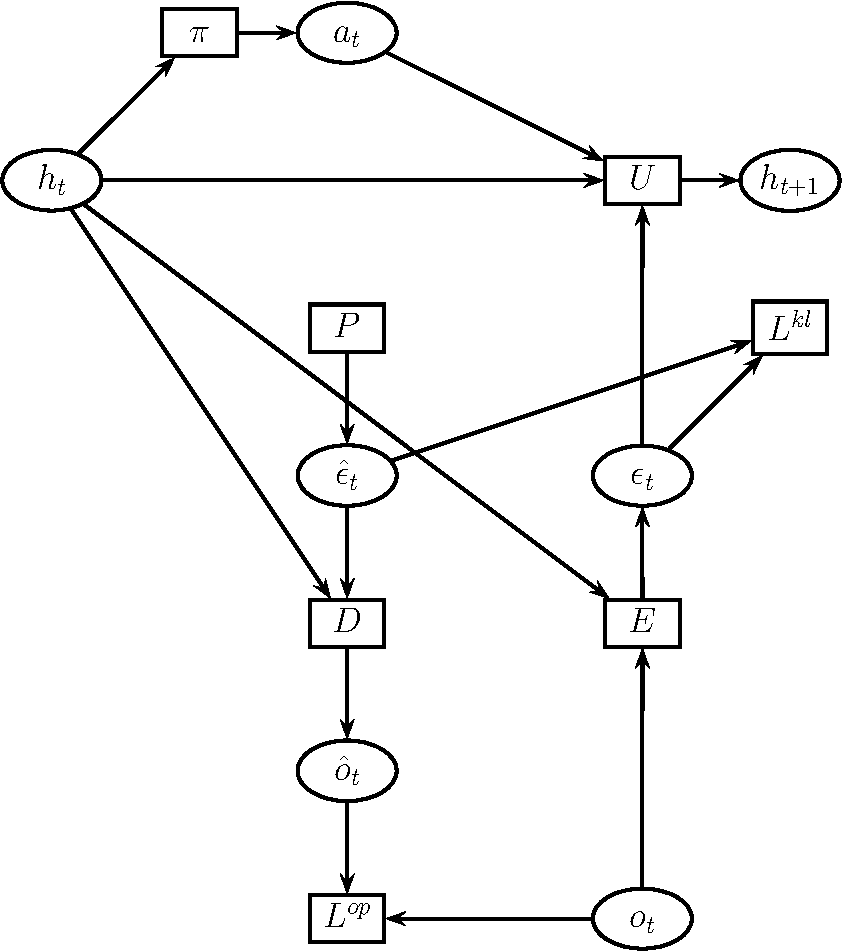
\includegraphics[height=4in]{figs/dreamer-noval}
\caption{
  Illustration of  Dreamer world model as a factor graph
  (so  squares are functions, circles are variables).
%  ($z_t$ is stochastic.)
  We have unrolled the forwards prediction for only 1 step.
  Also, we have omitted the reward prediction loss.
}
\label{fig:dreamer}
\end{figure}

\renewcommand{\latent}{\vepsilon}

In Dreamer, the
stochastic dynamic latent variables
in \cref{eqn:unrollLatent}
are replaced by deterministic dynamic latent
variables $\vh_t$,
since this makes the model easier to train.
(We will see that  $\vh_t$ acts like the posterior
over the hidden state at time $t-1$;
this is also the  prior predictive belief state
before we see $\vo_t$.)
A ``static'' stochastic variable $\latent_t$ is now generated
for each time step, and acts like a ``random effect''
in order to help generate the observations,
without relying on $\vh_t$ to store all of the necessary information.
(This simplifies the recurrent latent state.)
In more detail, Dreamer defines the following functions:\footnote{
%
To map from our notation to the notation in the paper,
see the following key:
%  $b_{t-1} \ra h_t$,
  $\vo_t \ra x_t$, 
  $U \ra f_{\phi}$ (sequence model),
  $P \ra p_{\phi}(\hat{z}_t|h_t)$ (dynamics predictor),ion model),
  $D \ra p_{\phi}(\hat{x}_t|h_t, \hat{z}_t)$  (decoder),
  $E \ra  q_{\phi}(\latent_t|h_t,x_t)$ (encoder).
}
\begin{itemize}
\item A hidden dynamics (sequence) model:  $\vh_{t+1}= U(\vh_{t}, \va_{t}, \latent_t)$
 \item A latent state prior: $\hat{\latent}_t \sim P(\hat{\latent}_t|\vh_{t})$ 
 \item A latent state decoder (observation predictor):
   $\hat{\vo}_t \sim D(\hat{\vo}_t|\vh_t,\hat{\latent}_t)$.
   \item A reward predictor: $\hat{r}_t \sim R(\hat{r}_t|\vh_t, \hat{\latent}_t)$
     \item A latent state encoder:  $\latent_t \sim E(\latent_t|\vh_{t}, \vo_t)$.
%   \item A value function: $v_{t-1} = V(\vh_t)$
  \item A policy function: $\va_t \sim \pi(\va_t|\vh_t)$
\end{itemize}
See \cref{fig:dreamer} for an illustration of the system.
%Note that the initial hidden state $\vh_0$ is assumed to be known;
%all subsequent hidden states $\vh_t$ can be computed
%deterministically given the past stochastic variables.

We now give a simplified explanation of how the world model is trained.
The loss has the form
\be
\loss^{\text{WM}} = \expectQ{
  \sum_{t=1}^T \beta_{o} \loss^o(\vo_t, \hat{\vo}_t) 
  + \beta_{z} \loss^z(\latent_t, \hat{\latent}_t)
  }{q(\latent_{1:T})}
\ee
where the $\beta$ terms are different weights for each loss,
and $q$ is the posterior over the latents, given by
\be
q(\latent_{1:T}|\vh_{0},\vo_{1:T},\va_{1:T})
 = \prod_{t=1}^T E(\latent_t|\vh_t,\vo_t) \delta(\vh_t-U(\vh_{t-1},\va_{t-1},\latent_{t-1}))
 \ee
The loss terms are defined as follows:
\begin{align}
  \loss^o &= -\ln D(\vo_t|\latent_t,\vh_t)\\
  \loss^z &= \KLpq{E(\latent_t|\vh_t,\vo_t))}{P(\latent_t|\vh_t)}) 
\end{align}
where we abuse notation somewhat,
since $\loss^z$ is a function of two distributions,
not of the variables $\latent_t$ and $\hat{\latent}_t$.

In addition to the world model loss, we have the following
actor-critic losses
\begin{align}
  \loss^{\text{critic}}
  &= \sum_{t=1}^T (V(\vh_t) - \stopgrad(G_t^{\lambda}))^2 \\
  \loss^{\text{actor}}
   &= -\sum_{t=1}^T \stopgrad((G_t^{\lambda}-V(\vh_t))) \log \pi(\va_t|\vh_t)
  \end{align}
where $G_t^{\lambda}$ is the GAE estimate of the reward to go:
\be
G_t^{\lambda} = r_t + \gamma\left( (1-\lambda) V(\vh_t) + \lambda G_{t+1}^{\lambda} \right) 
\ee

\eat{
\newcommand{\tpred}{\text{pred}}
\newcommand{\tdyn}{\text{dyn}}
\newcommand{\trep}{\text{rep}}



The world model is trained to minimize the following loss:
\be
\loss = \expectQ{
  \sum_{t=1}^T \beta_{\tpred} \loss_{\tpred}
  + \beta_{\tdyn} \loss_{\tdyn}
  + \beta_{\trep} \loss_{\trep}
  }{q(\vz_{1:T}|\vh_{0:T},\vo_{1:T})}
\ee
where the $\beta$ terms are different weights for each loss.
The loss terms are defined as follows:
\begin{align}
  \loss_{\tpred} &= -\ln D(\vo_t|\vz_t,\vh_t)
  - \ln R(r_t|\vz_t,\vh_t) \\
  \loss_{\tdyn} &= \max(1, \KLpq{\stopgrad(E(\vz_t|\vh_t,\vo_t))}{P(\vz_t|\vh_t)}) \\
  \loss_{\trep} &= \max(1, \KLpq{E(\vz_t|\vh_t,\vo_t)}{\stopgrad(P(\vz_t|\vh_t))})
\end{align}
where $\stopgrad$ is the stop gradient operator.
Here $\loss_{\tpred}$ is the observation prediction loss;
$\loss_{\tdyn}$ is the dynamics loss, that trains the sequence
model to predict the (frozen) latent encoding;
and $\loss_{\trep}$ is the representation loss,
that trains the latent encoder to be predictable
by the (frozen) dynamics model.
The use of the $\max(1,KL)$ expression is to ensure
that the KL loss does not have to go all the way to 0,
which can cause latent variable collapse.
the value of 1 nat (about 1.44 bits) corresponds
to the \keywordDef{free bits} of the encoding
\citep{kingma2016improving}.
}

\eat{
A recent extension of the PlaNet paper,
known as \keywordDef{Dreamer},
was proposed in \citep{dreamer}.
In this paper, the online MPC planner is replaced
by a policy network, $\policy(\va_t|\vz_t)$,
which is learned using
gradient-based actor-critic in latent space.
%\eat{
%More precisely, Dreamer
%learns a Markovian
%inference model $q(\vz_t|\vz_{t-1},\va_{t-1},\vs_t)$
%(which they call the ``representation model''),
%the transition model $p(\vz_t|\vz_{t-1},\va_{t-1})$,
%reward model $p(r_t|\vz_t)$,
%observation model $p(\vs_t|\vz_t)$,
% policy $\policy(\va_t|\vz_t)$,
% and value function $V(\vz_t)$.
%}
The inference and generative models
are trained by maximizing the ELBO,
as in PlaNet.
(They also tried replacing the reconstruction
loss with noise contrastive estimation
which avoids the need to
generate pixels; however,  this gave worse results.)
The policy and  value function are trained with actor-critic
with GAE estimation (see \cref{algo:AC}).
They show that Dreamer gives better results
than PlaNet, presumably because they
learn a policy to optimize the
long term reward (as estimated by the value function),
rather than relying on MPC
based on short-term rollouts.
}

There have been several extensions to the original Dreamer paper.
\keyword{DreamerV2} \citep{dreamerv2}
adds categorical (discrete) latents and  KL balancing between prior
and posterior estimates.  
This was the
first imagination-based agent to outperform humans in Atari games.
\keyword{DayDreamer} \citep{dayDreamer}
applies DreamerV2 to real robots.
\keyword{DreamerV3} \citep{dreamerv3}
builds upon DreamerV2 using various tricks --- such as symlog
encodings\footnote{
%
The symlog function is defined as
$\text{symlog}(x) = \text{sign}(x)\ln(|x|+1)$,
and its inverse is
$\text{symexp}(x) = \text{sign}(x)(\exp(|x|)-1)$.
The symlog function squashes large positive and negative values,
while preserving small values.
} %
for the reward, critic, and decoder ---
to enable more stable optimization and domain independent
choice of hyper-parameters.
It was the first method to create diamonds in the Minecraft
game without requiring human demonstration data.
(However, reaching this goal took 17 days of training.)
\citep{Lin2024} extends DreamerV3 to also model language
observations.


Variants of Dreamer such as TransDreamer \citep{transDreamer}
 and STORM \citep{storm}  have also been
 explored, where transformers replace the recurrent network.
The  \keyword{DreamingV2} paper of \citep{dreamingV2}
replaces the generative loss
with a non-generative self-prediction loss (see \cref{sec:SPR}).

\subsubsection{Iris}
\label{sec:iris}

The \keywordDef{Iris} method
of \citep{iris} follows the MBRL paradigm,
in which it alternates beween
(1) learning a world model
using real data $D_r$
and then  generate imaginary rollouts $D_i$ using the WM,
and (2)
learning the policy given $D_i$
and collecting new data $D_r'$ for learning.
In the model learning stage,
Iris learns a discrete latent
encoding using the VQ-VAE method,
and then  fits a transformer dynamics
model to the latent codes.
In the policy learning stage, it uses actor critic methods.
The \keywordDef{Delta-Iris}
method of \citep{delta-iris}
extends this by training the model to only predict
the delta between neighboring frames.
Note that, in both cases, the policy has the form $a_t=\pi(\vo_t)$,
where $\vo_t$ is an image, so the
the rollouts need to ground to pixel space, and cannot only
be done in latent space.

 



\subsection{Non-generative world models}
\label{sec:nongen}
\label{sec:MBRLnongen}


In \cref{sec:MBRLgame}, we argued that, if we can learn a sufficiently accurate world
model, then solving for the optimal policy in simulation will give
a policy that is close to optimal in the real world.
However, a simple agent may not be able to capture the full complexity
of the true environment;
this is called the ``\keywordDef{small agent, big world}'' problem
\citep{Dong2022,bitByBit,Arumugam2024,Kumar2024}.

Consider what happens when the agent's model is misspecified (i.e., it cannot
represent the true world model), which is nearly always the case.
The agent will train its model
to reduce state (or observation) prediction error,
by minimizing $\lossfn(\hat{M}, \mu_M^{\pi})$.
However, not all features of the state are useful for planning.
For example, if the states are images, a dynamics model
with limited representational capacity may choose
to focus on predicting the background pixels
rather than more control-relevant features, like small moving
objects, since predicting the background reliably
reduces the MSE more.
This is due to ``\keywordDef{objective mismatch}''
\citep{Lambert2020RL,Wei2023MBRL},
which refers to the discrepancy between the way a
model is usually trained (to predict the observations)
vs the way its representation is used for control.
To tackle this problem, in this section we discuss methods
for learning representations and models that don't rely on
predicting all the observations.
Our presentation is based in part
on   \citep{Ni2024} (which in turn builds on
\citep{Subramanian2022}).
See \cref{tab:WM} for a summary of some of the methods
we will discuss.



\begin{table}
  \centering
  \begin{tabular}{llll}
    Loss & Policy & Usage & Examples \\ \hline
    OP & Observables & Dyna & Diamond \citep{Alonso2024}, Delta-Iris \citep{delta-iris} \\
    OP & Observables & MCTS & TDM  \citep{Schubert2023} \\
    OP & Latents & Dyna & Dreamer \citep{dreamerv3} \\
    RP, VP, PP & Latents & MCTS & MuZero \citep{Schrittwieser2020} \\
    RP, VP, PP, ZP & Latents & MCTS & EfficientZero  \citep{efficientZero} \\
    RP, VP, ZP  & Latents & MPC-CEM & TD-MPC \citep{Hansen2022} \\
    VP, ZP  & Latents & Aux. &  Minimalist \citep{Ni2024} \\
    VP, ZP & Latents & Dyna & DreamingV2  \citep{dreamingV2} \\
    VP, ZP, OP & Latents & Dyna & AIS  \citep{Subramanian2022}\\
    POP & Latents & Dyna & Denoised MDP  \citep{Wang2022}
  \end{tabular}
  \caption{Summary of some world-modeling methods.
    % SPR \citep{Schwarzer2021},
    The ``loss'' column refers to the loss used to train
    the latent encoder (if present) and the dynamics model
    (OP = observation prediction, ZP = latent state prediction,
    RP = reward prediction, VP = value prediction,
    PP = policy prediction, POP = partial observation prediction).
    The ``policy'' column refers to the input that is passed
    to the policy.
    (For MCTS methods, the policy is just used as a proposal
    over action sequences to initialize the search/ optimization process.)
    The ``usage'' column refers to how to the world model is used:
        for  background planning (which we call ``Dyna''),
        or for decision-time planning (which we call ``MCTS''),
        or just as an auxiliary loss on top of standard policy/value
        learning (which we call ``Aux'').
        Thus Aux methods are single-stage (``end-to-end''), whereas the other
        methods alternate are two-phase, and alternate between improving the world model
    and then using it for improving the policy (or searching for the optimal action).
    }
  \label{tab:WM}
  \end{table}


\subsubsection{Value prediction}
\label{sec:valueEquivalence}

\newcommand{\hist}{\data}

Let $\hist_t =(\hist_{t-1},\va_{t-1},r_{t-1},\vo_t)$ be the observed history at time $t$,
and let $\vz_t = \phi(\hist_t)$ be a latent representation (compressed encoding)
of this history, where $\phi$ is called an encoder or a \keywordDef{state abstraction}
function. We will train the policy $\va_t=\pi(\vz_t)$ in the usual way,
so our focus will be on how to learn good latent representations.

An optimal representation $\vz_t=\phi(\hist_t)$ is a sufficient statistic
for the optimal action-value function $Q^*$.
Thus it satifies the \keywordDef{value equivalence} principle
\citep{Li2006,Castro2011,Grimm2020,Grimm2022,Alver2023,Alver2024},
which says  that two states $s_1$ and $s_2$ are  value equivalent
(given a policy)
if $V^{\pi}(s_1) = V^{\pi}(s_2)$.
In particular, if the representation is optimal,
it will satisfy value equivalence wrt the optimal policy,
i.e.,
if $\phi(\hist_i)=\phi(\hist_j)$ then $Q^*(\hist_i,a)=Q^*(\hist_j,a)$.
We can train such a representation function by using
its output $\vz=\phi(\hist)$ as input to the Q function
or to the policy.
(We call such a loss \keywordDef{VP}, for value prediction.)
This will cause the model to focus
its representational power on the relevant parts of the observation
history.


Note that there is a stronger property than value equivalence
called \keywordDef{bisimulation}
\citep{Givan2003}.
This says that two states $s_1$ and $s_2$ are bisimiliar if
$P(s'|s_1,a) \approx P(s'|s_2,a)$ and $R(s_1,a) = R(s_2,a)$.
From this, we can derive a continuous measure called the
\keywordDef{bisimulation metric} \citep{Ferns2004}.
This has the advantage (compared to value equivalence)
of being policy independent, but the disadvantage that it can be 
harder to compute  \citep{Castro2020mdp,Zhang2021},
although there has been recent progress on computaitonally
efficient methods such as MICo \citep{Castro2021}
and KSMe \citep{Castro2023}.



\eat{
\subsection{Value equivalence}
\label{sec:valueEquivalence}


Rather than training a (possibly latent) model to generate every pixel
in an image,
and then learning the corresponding latent dynamics,
we can train a dynamics model to only predict
quantities that are relevant to the task at hand.
This is formalized in the
principle of \keywordDef{value equivalence},
which 
says that two models are equally good if they give
rise to the same optimal  value function
\citep{Grimm2020,Grimm2022,Alver2023,Alver2024}.
More precisely, let the value function for a model $M=(T,R)$
with policy $\pi$ be
\be
V_{M}^{\pi}(s) = \expectQ{\sum_{t=0}^{\infty} \gamma^t R(s_t,a_t)|s_0=s}{\pi,T}
 \ee
Let $\pi^*_M$ be the optimal policy for this model.
We say that   $\MVE$ is value equivalent (VE) to $\Mtrue$ if
\be
V_{\Mtrue}^{\pi^*_{\MVE}} = V^{\pi^*_{\Mtrue}}_{\Mtrue}
\ee
In practice we may not be find a VE model $\MVE$
that is smaller/simpler than $\Mtrue$,
so  \citep{Arumugam2022} propose a notion of approximate value equivalence,
that allows us to trade off model simplicity against
distortion in the induced value function.
}



\subsubsection{Self prediction}
\label{sec:SPR}
\label{sec:self-predictive}

Unfortunately, in problems with sparse reward,
predicting the value may  not provide enough of a feedback signal
to learn quickly. Consequently it is common to augment
the training with a \keywordDef{self-prediction} loss
where we train $\phi$ to ensure
the following condition hold:
\begin{align}
  \exists M \myst  \expectQ{\vz'|\hist,a}{M^*} &=
  \expectQ{\vz'|\phi(\hist),a)}{M} \;\; \forall \hist,a
\end{align}
where the LHS is the predicted mean
of the next latent state under the true model,
and the RHS is the predicted mean under the learned
dynamics model.
We call this the \keywordDef{EZP}, which stands for expected $\vz$ prediction.\footnote{
%
In \citep{Ni2024}, they also describe the ZP loss,
which requires predicting the  full distribution over $\vz'$
using a stochastic transition model.
This is strictly  more powerful, but somewhat more complicated,
so we omit it for simplicity.
}

A trivial way to minimize the (E)ZP loss is for the embedding
to map everything to a constant vector, say $E(\hist)=\vzero$,
in which case $\vz_{t+1}$ will be trivial for  the
dynamics model $M$ to predict.
However this is not a useful representation.
This problem is \keywordDef{representational collapse}
\citep{Jing2022collapse}.
Fortunately,
we can provably prevent collapse (at least for linear encoders)
by using a frozen target network 
\citep{Tang2023,Ni2024}. That is, we use the following auxiliary
loss
\be
\loss_{\text{EZP}}(\vphi,\vtheta;\hist,a,\hist')
= ||M_{\vtheta}(E_{\vphi}(\hist,a)) - E_{\overline{\vphi}}(\hist')||_2^2
\ee
where 
\be
\overline{\vphi}=\rho \overline{\vphi} + (1-\rho) \stopgrad(\vphi)
\ee
is the (stop-gradient version of) the EMA
of the encoder weights.
(If we set $\rho=0$, this is called a detached network.)


\begin{figure}
\centering
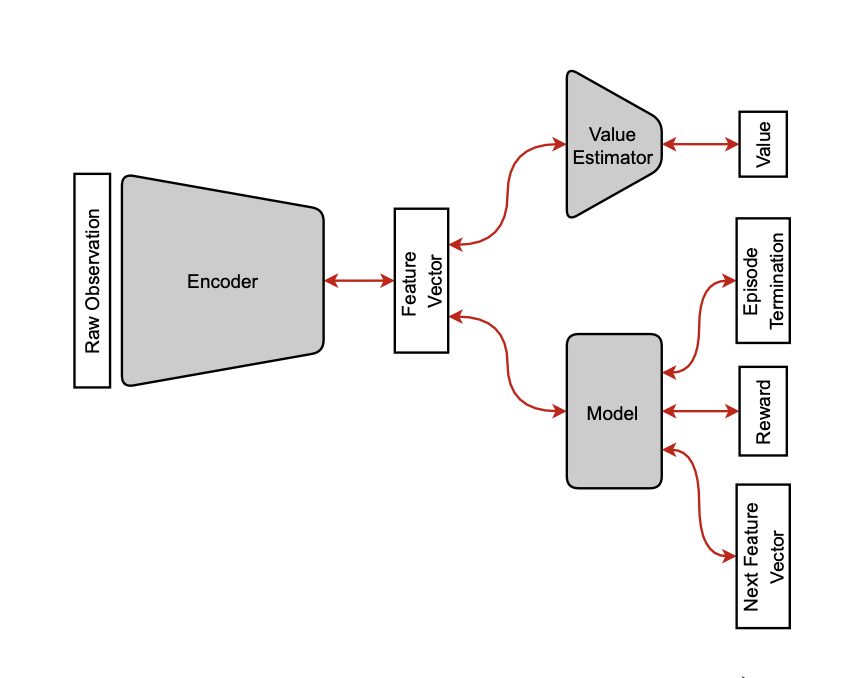
\includegraphics[height=2.5in]{figs/MBRLtargets.png}
\caption{
  Illustration of  an encoder $\vz_t=E(\vo_t)$,
  which is passed to a value estimator $v_t=V(\vz_t)$,
  and a world model, which predicts
  the next latent state $\hat{\vz}_{t+1}=M(\vz_t,a_t)$,
  the reward $r_t=R(\vz_t,a_t)$,
  and the termination (done) flag, $d_t=\done(\vz_t)$.
  \figtaken{Figure C.2 of \citep{Alver2023}.}
\figthanks{Doina Precup}.
}
\label{fig:MBRLtargets}
\end{figure}

We can also train the latent encoder to predict the reward.
Formally, we want to ensure we can satisfy the following condition,
which we call \keywordDef{RP} for ``reward prediction'':
\begin{align}
%  \exists M \myst P(\vz'|\hist,a) &= M(\vz'|\phi(\hist), a) \forall \hist,a,\vz
%   & \text{ZP} \\
  \exists R \myst  \expectQ{r|\hist,a}{R^*} &=
  \expectQ{r|\phi(\hist),a)}{R} \;\; \forall \hist,a
\end{align}
See \cref{fig:MBRLtargets} for an illustration.
In \citep{Ni2024}, they prove that a representation
that satisfies ZP and RP is enough to satisfy value equivalence
(sufficiency for $Q^*$).

Methods that optimize ZP and VP loss
have been used in many papers,
such as 
\keywordDef{Predictron}  \citep{predictron},
\keywordDef{Value Prediction Networks} \citep{Oh2017},
\keywordDef{Self Predictive Representations} (SPR)
\citep{Schwarzer2021},
\keywordDef{Efficient Zero}
(\cref{sec:efficientZero}),
\keywordDef{BYOL-Explore}
(\cref{sec:BYOL}),
etc.


\subsubsection{Policy prediction}


The value function and reward losses may be too sparse
to learn efficiently. Although self-prediction loss can help somewhat,
it does not use any extra information from the environment as feedback.
Consequently it is natural to consider other kinds of prediction
targets for learning the latent encoder (and dynamics).
When using MCTS, it is possible compute what the policy should
be for a given state, and this can be used as a prediction
target for the reactive policy $a_t=\pi(\vz_t)$,
which in turn can be used as a feedback signal for the latent
state. This method is used by MuZero (\cref{sec:muZero})
and EfficientZero (\cref{sec:efficientZero}).



\subsubsection{Observation prediction}

Another natural target to use for learning the encoder
and dynamics is the next observation,
using a one-step version of \cref{eqn:unroll}.
Indeed, \citep{Ni2024} say that a representation $\phi$ satsifies
the \keywordDef{OP} (observation prediction)
criterion if it satisfies the following condition:
\begin{align}
  \exists D \myst  p^*(\vo'|\hist,a) = D(\vo'|\phi(\hist),a)
\;\; \forall \hist,a
\end{align}
where $D$ is the decoder.
In order to repeatedly apply this, we need to be able
to update the encoding $\vz=\phi(\hist)$ in a recursive
or online way. Thus we must also satisfify
the following recurrent encoder condition,
which \citep{Ni2024}
call \keywordDef{Rec}:
\begin{align}
  \exists U \myst  \phi(\hist') = U(\phi(\hist), a, \vo')
\;\; \forall \hist,a,\vo'
\end{align}
where $U$ is the update operator.
Note that belief state updates (as in a POMDP)
satisfy this property.
Furthermore, belief states are a sufficient statistic
to satisfy the OP condition.
See \cref{sec:MBRLlatent} for a discussion of generative models
of this form.
However, there are other approaches to partial
observability which work directly
in prediction space (see \cref{sec:PSR}).

\subsubsection{Partial observation prediction}

We have argued that predicting all the observations
is problematic, but not predicting them is also problematic.
A natural compromise is to predict some of the observations,
or at least sone function of them.
This is known as a \keywordDef{partial world model}
(see e.g., \citep{Alver2023}).

The best way to do this is an open research problem.
A simple approach would be to predict all the observations,
but put a penalty on the resulting OP loss term.
A more sophisticated approach would be to structure the latent
space so that we distinguish latent variables
that are useful for learning $Q^*$ (i.e., which affect the reward
and which are affected by the agent's actions)
from other latent variables that are needed to explain
parts of the observation but otherwise are not useful.
We can then impose an  information bottleneck
penalty on the latter, to prevent the agent
focusing on irrelevant observational details.
(See e.g., the \keywordDef{denoised MDP} method
of \citep{Wang2022}.)


\subsubsection{BYOL-Explore}
\label{sec:BYOL}

\begin{figure}
\centering
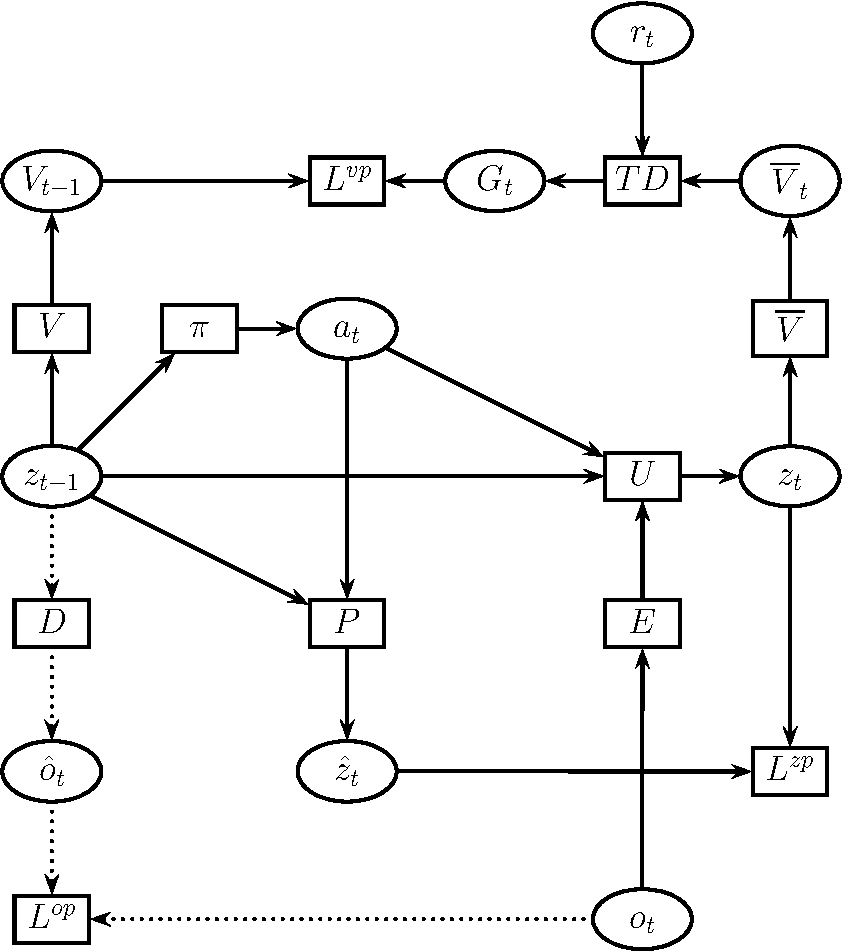
\includegraphics[height=4in]{figs/byol2}
\caption{
  Illustration of (a simplified version of)  the BYOL-Explore architecture,
  represented as a factor graph
  (so squares are functions, circles are variables).
  The dotted lines represent an optional observation
  prediction loss.
  The map from notation in this figure to the paper is as follows:
  $U \ra h^c$ (closed-loop RNN update),
  $P \ra h^o$ (open-loop RNN update),
  $D \ra g$ (decoder),
  $E \ra f$ (encoder).
  We have unrolled the forwards prediction for only 1 step.
  Also, we have omitted the reward prediction loss.
  The $\overline{V}$ node is the EMA version of the value function.
  The TD node is the TD operator.
}
\label{fig:byol}
\end{figure}

As an example of the above framework,
consider the \keywordDef{BYOL-Explore} paper
\citep{BYOLexplore}, which uses a  non-generative world model
trained with ZP and VP loss.
(BYOL stands for ``build your own latent''.)
See  \cref{fig:byol} for 
the computation graph,
which we see is slightly simpler than the
Dreamer computation graph in \cref{fig:dreamer}
due to the lack of stochastic latents.
%(in BYOL, the $\vz_t$ variables are updated using an RNN).
In addition to using self-prediction loss to help train the latent
representation, the error in this loss can be used
to define an intrinsic reward, to encourage the agent
to explore states where the model is uncertain.
See \cref{sec:intrinsic} for further discussion of this topic.



\eat{
In  \citep{Weber2017nips}, they train a model
to predict future states and rewards, and then use
the hidden states of this model as additional
context for a policy-based learning method.
This can help overcome partial observability.
They call their method \keywordDef{imagination-augmented agents}.
}

%(discussed in \cref{sec:MCTS})
%and TD-MPC (discussed in \cref{sec:TDMPC}).
%trains a latent world model to predict the  reward,
%policy and value function.


\eat{
\subsection{Self-prediction}
\label{sec:self-predictive}
\label{sec:SPR}

Since the reward and value of a state are just scalars,
predicting them  is often an insufficient feedback signal to train the
latent representation
(especially in sparse reward problems).
Fortunately we can add  additional losses or auxiliary signals,
to regularize the representation learning problem
\citep{Jaderberg2017iclr}.
This can help in situations when rewards are sparse or absent.

%as we discuss in \cref{sec:GVF} on general value functions.
In general it can be difficult to decide what features
are worth modeling.
But a common approach is to predict the next latent state,
in addition to the reward and value,
as shown in \cref{fig:MBRLtargets}.
This is called a \keywordDef{self predictive representation} or \keywordDef{SPR}.
That is, we add a loss of the form $\loss(\hat{\vz}_{t+1}, \vz_{t+1})$,
where $\vz_{t+1}=E(\vo_{t+1})$ is the actual  next latent state,
$\hat{\vz}_{t+1}=M(\vz_t,a_t)$ is  the predicted  next latent state,
and the loss function is something like cosine distance in embedding space.
We use this loss not only to train the dynamics model $M$,
but also the encoder $E$.
A trivial way to minimize this loss wrt $E$ is for the embedding
to map everything to a constant vector, say $E(\vo)=\vzero$,
in which case $\vz_{t+1}$ will be trivial for  $M$
to predict.
However this is not a useful representation.
This problem is \keywordDef{latent representational collapse}
\citep{Jing2022}.
Fortunately,
we can provably prevent collapse (at lest for linear encoders)
by using a frozen target network and bilevel optimization
\citep{Tang2023,Ni2024}.
(The reward and value losses also help prevent total collapse.)
}



\eat{
\subsubsection{BYOL-Explore}

Self-prediction is also used
 in the \keyword{BYOL-Explore} paper
 \citep{BYOLexplore},
 which is used to create an intrinsic reward.
%the \keyword{Efficient Zero} paper  \citep{efficientZero}
%(summarized in \cref{sec:MCTS}),
}


\eat{
As with  other contrastive losses used in self-supervised learning
(see \cref{sec:contrastiveLoss}),
we need to  prevent the embedding from collapsing to a trivial
function (e.g. $\phi(\vo_t)=\vzero_t$), which would be easy
to predict.
(This is similar to the problems caused by bootstrapping
in the context of off-policy RL, see \cref{sec:deadlyTriad}.)
The standard approach is to use tricks such as target networks
and stop gradients, as discussed in \cref{sec:targetNetwork}.
Alternatively, we can use non-contrastive or negative-free
methods (\cref{sec:negative-free});
for example,  \citep{Robine2023}
use  VICReg \citep{VICreg} inside a Dyna setup.
}


\eat{
It is also possible to use non-contrastive, but still non-generative,
methods for learning the latents. For example,
\keywordDef{DreamerPro} \citep{dreamerPro}
uses an approach based on ``prototypical representations'',
derived from the hidden state of the RNN dynamics model.
The \keywordDef{IFactor} approach of \citep{iFactor}
partitions the the latent factors into four groups,
based on whether they are predictive of reward or not,
and based on whether they are influenced by the actions or not.
}


\eat{
The action-value functions for the intermediate nodes
in the search tree are represented by deep neural networks,
and updated using temporal difference
methods that we discuss in \cref{sec:valueBased}.
MCTS can also be applied to many other kinds of seqential decision problems,
such as experiment design for
sequentially creating molecules~\citep{Segler2018}.
}



%%%%

\eat{
\subsection{Differentiable planning}
\label{sec:differentiable-planning}


One solution to the objective mismatch  problem is to use
\keywordDef{differentiable planning},
in which we combine model learning and policy learning together,
and train them jointly end-to-end,
rather than in an alternating two-player fashion.
In particular, we can solve try to optimize
\begin{equation*}
  \min_{\hat{M}, Q} \expectQ{(R(s,a) + \gamma V(s') - Q(s,a))^2}
      {(s,a,s')    \sim \data}
  \end{equation*}
where  $s'=\hat{M}(s,a)$ is the learned dynamics model,
subject to the constraint that the value function
is derived from the model using
\begin{equation*}
V(s) = \argmax_{a(0:K)} \expectQ{\sum_{k=0}^{K-1}
  \gamma^k R(s_k,a_k) + \gamma^K V(s_K) | S_0=s}{\hat{M}}.
\end{equation*}
This bilevel optimization problem was first proposed
in the \keywordDef{TreeQN} paper
\citep{treeQN}.
In \citep{Amos2019DCEM} they proposed a version of
this for continuous actions based on the differentiable
CEM method (see \cref{sec:CEM}).
In \citep{Nikishin2022,Bansal2023}
they propose to use implicit differentation to avoid
explicitly unrolling the inner optimization.
 
\subsection{Variational inference}
\label{sec:VMBPO}
\label{sec:ALM}

In this section, we present another solution to the objective
mismatch problem.
It is an extension of the framework of
\cref{sec:inferRL}, where we formulate control (RL)
as an inference problem,
where the goal is to infer the posterior over states and actions
that maximizes the log probability of observing
the sequence of optimality variables
$O_{t}=1$, where $p(O_t=1|s_t,a_t) = \exp(R(s_t,a_t))$.
In \cref{sec:inferRL},  we only optimize the parameters of the policy,
treating the samples as coming from the true dynamics model,
resulting in the model-free SAC algorithm.
Here we jointly optimize over the policy $\pi$
and the dynamics  $M$, allowing for planning and policy
learning ``in imagination''.
We follow the presentation of
\citep{Wei2023MBRL},
which should be consulted for more details.


Using standard methods from variational inference (see \cref{chap:VI}),
we can derive the following  lower bound
on the log likelihood
\begin{equation*}
  \log p(O_{0:\infty}=1) \geq
  \expectQ{\sum_{t=0}^{\infty} R(s_t,a_t)}{Q(\tau)}
  -\KLpq{Q(\tau)}{P(\tau)}
\end{equation*}
In the above,
$P(\tau)$ is
the true distribution over state and action trajectories, given by
\begin{equation*}
  P(\tau) = \mu(s_0) \prod_{t=0}^{\infty} M(s_{t+1}|s_t,a_t)
  P(a_t|s_t)
\end{equation*}
where $P(a|s)$ is the behavior policy (which we may approximate as uniform),
$\mu(s_0)$ is the distribution over starting states,
and $M$ is the true dynamics model.
Furthermore, $Q(\tau)$ is the approximate distribution
given by
\begin{equation*}
  Q(\tau) = \mu(s_0) \prod_{t=0}^{\infty} \hat{M}(s_{t+1}|s_t,a_t)
  \pi(a_t|s_t)
\end{equation*}
We can therefore rewrite the lower bound maximization problem
as follows:
\begin{equation*}
  \max_{\hat{M},\pi}
  \expectQ{\sum_{t=0}^{\infty} \gamma^t\left(
    R(s_t,a_t) + \log \frac{P(a_t|s_t)}{\pi(a_t|s_t)}
    + \log \frac{M(s_{t+1}|s_t,a_t)}{\hat{M}(s_{t+1}|s_t,a_t)}\right)
    }{Q(\tau)}
\end{equation*}
\eat{
In \citep{Chow2021},
they show that the optimal variational dynamics and policy have the
form
\begin{eqnarray*}
  \hat{M}(s'|s,a)& \propto& \exp(V(s') + \log M(s'|s,a)) \\
  \pi(a|s) &\propto& \exp(Q(s,a) + \log P(a|s))
\end{eqnarray*}
where
we have used the following Bellman-like equation:
\begin{equation*}
Q(s_t,a_t) = R(s_t,a_t) + \log \frac{P(a_t|s_t)}{\pi(a_t|s_t)}
+ \expectQ{V(s_{t+1}) +
  \log \frac{M(s_{t+1}|s_t,a_t)}
       {\hat{M}(s_{t+1}|s_t,a_t)}
       }
    {\hat{M}(s_{t+1}|s_t,a_t)}
\end{equation*}
and we define $V(s) = \argmax_a Q(s,a)$.
}
We can approximate the  density ratio
$\frac{M(s_{t+1}|s_t,a_t)}{\hat{M}(s_{t+1}|s_t,a_t)}$
using a binary classifier,
as discussed in \cref{sec:class_probability_estimation}.
In \citep{Chow2021}, they call this method
\keywordDef{VMBPO}
for ``Variational Model-Based Policy Optimization''.


In \citep{Eysenbach2022}, they derive a tighter bound,
by defining the optimality variable based on the entire trajectory,
$p(O=1|\tau) = R(\tau) = \sum_{t=1}^{\infty} \gamma^t R(s_t,a_t)$.
This gives rise to the following simpler lower bound:
\begin{eqnarray*}
  \log p(O=1) &= \log \int_{\tau} P(O=1,\tau)
  = \log \expectQ{P(O=1|\tau)}{P(\tau)}
  \geq \expectQ{\log R(\tau) + \log P(\tau) - \log Q(\tau)}{Q(\tau)}
\end{eqnarray*}
This gives rise to   an objective that is the same
as in VMBPO but $R(s,a)$ is replaced by $\log R(s,a)$.
They call their method
\keywordDef{Mismatched No More},
so-called since it solves the model-policy
mismatch.

In \citep{Ghugare2022}
they extend MNM to work with images (and other high dimensional states)
by learning a latent encoder $\hat{E}v(z_t|s_t)$
as well as latent dynamics $\hat{M}(z_{t+1}|\z_t,a_t)$.
The trajectories are now defined over observed states, latent states,
and actions, and the objective becomes the following:
\begin{equation*}
  \max_{\hat{M},\hat{E},\pi}
  \expectQ{\sum_{t=0}^{\infty} \gamma^t\left(
    \log R(s_t,a_t) + \log \frac{P(a_t|s_t)}{\pi(a_t|s_t)}
    + \log \frac{\hat{E}(z_{t+1}|s_{t+1})}{\hat{M}(z_{t+1}|z_t,a_t)}\right)
    }{Q(\tau)}
\end{equation*}
They call their method
\keywordDef{Aligned Latent Models}.\footnote{
%
Note that the above objective corresponds to a simplified
form of the offline RL
objective in Appendix A.7 of \citep{Ghugare2022}.
It is simplified because we  use Monte Carlo rollouts
rather than a $K$-step bootstrap estimate of the return.
Note that,
in the offline setting, the $P(a_t|s_t)$ term can be learned using  behavior cloning.
However, it is also possible to derive an online RL objective
in which $P(a_t|s_t) = \pi(a_t|s_t)$, so this term cancels out.
See \citep{Ghugare2022} for details.
}
We note that the final term is similar to
other self-predictive representation learning 
methods discussed in \cref{sec:self-predictive},
and the authors use a simlar target network approach for the
encoder $E$ to ensure stability of training.

}





%\section{Beyond one-step models: predictive representations}
\label{sec:beyond}
\label{sec:successor}


The ``world models'' we described in \cref{sec:WM}
are \keywordDef{one-step models} of the form $p(s'|s,a)$,
or $p(z'|z,a)$ for $z=\phi(s)$, where $\phi$ is a state-abstraction
function.
However, such models are problematic when it comes to predicting
many kinds of future events, such as ``will a car pull in front of me?''
or ``when will it start raining?'',
since it is hard to predict exactly when these events will occur,
and these events may correspond to many different ``ground states''.
In principle we can roll out many possible long term futures,
and apply some abstraction function to  the resulting
generated trajectories to extract features of interest,
and thus derive a predictive model of the form $p(t', \phi(s_{t+1:t'})|s_t,\pi)$,
where $t'$ is the random duration of the sampled trajectory.
However, it would be more
efficient if we could directly predict this distribution
without having to know the value of $t'$,
and without having to predict all the details of all the
intermediate future states,
many of which will be irrelevant given the abstraction function $\phi$.
This motivates the study of multi-step world models,
that predict multiple steps into the future,
either at the state level, or at the feature level.
These are called \keywordDef{predictive representations},
and are a compromise between standard model-based RL
and model-free RL, as we will see.
Our presentation on this topic is based on 
\citep{Carvalho2024}.
% https://julien-vitay.net/post/successor_representations/
(See also \cref{sec:HRL}, where we discuss the related topic
of temporal abstraction from a model-free perspective.)

\subsection{General value functions}
\label{sec:GVF}

The value function is based on  predicting the sum of expected
discounted future rewards.
But the reward is just one possible signal of interest we can extract from the environment.
We can generalize this by considering a \keywordDef{cumulant}
$C_t \in \real$, which is some scalar of interest derived from the state or observation
(e.g., did a loud bang just occur? is there a tree visible in the image?).
We then define the \keywordDef{general value function} or \keywordDef{GVF}
as follows \citep{GVF}:
\be
V^{\pi,C,\gamma}(s) = \expect{
  \sum_{t=0}^{\infty} \gamma^t C(s_{t+1}) \vert s_0=s, a_{0:\infty} \sim \pi}
\ee
If $C(s_{t+1})=R_{t+1}$, this reduces to the value function.\footnote{
%
This follows the convention  of \citep{Suttonv2},
where we write $(s_t, a_t, r_{t+1}, s_{t+1})$
to represent the transitions, since
$r_{t+1}$ and $s_{t+1}$ are both generated
by applying $a_t$ in state $s_t$.
}
However, we can also define the GVF to predict components
of the observation vector; this is called \keywordDef{nexting} \citep{Modayil2014},
since it refers to next state prediction at different timescales.

\subsection{Successor representations}
\label{sec:SR}
\label{sec:PSR}


In this section we consider a variant of GVF
where the cumulant corresponds
to a state occupancy vector $C(s_{t+1}) = \ind{s_{t+1}=\tilde{s}}$,
which provides a dense feedback signal.
This give us the \keywordDef{successor representation} or \keywordDef{SR}
\citep{Dayan1993}:
\be
M^{\pi}(s,\tilde{s}) = \expect{
  \sum_{t=0}^{\infty} \gamma^t \ind{s_{t+1}=\tilde{s}} \vert S_0=s}
\ee
If we define the policy-dependent state-transition matrix by
\be
T^{\pi}(s,s') = \sum_a \pi(a|s) T(s'|s,a)
\ee
then the SR matrix can be rewritten as
\be
\vM^{\pi} = \sum_{t=0}^{\infty} \gamma^t [\vT^{\pi}]^{t+1}
= \vT^{\pi} (\vI - \gamma \vT^{\pi})^{-1}
\ee
Thus we see that the SR replaces information about
individual transitions with their cumulants,
just as the value function replaces individual rewards
with the reward-to-go.

Like the value function, the SR obeys a Bellman equation
\begin{align}
  M^{\pi}(s,\tilde{s})
  &= \sum_a \pi(a|s) \sum_{s'}
T(s'|s,a)\left( \ind{s'=\tilde{s}} + \gamma M^{\pi}(s',\tilde{s})
\right) \\
   &= \expect{\ind{s'=\tilde{s}} + \gamma M^{\pi}(s',\tilde{s})}
\end{align}
Hence we can learn an SR using a TD update of the form
\begin{align}
  M^{\pi}(s,\tilde{s}) &\leftarrow
  M^{\pi}(s,\tilde{s}) + \eta 
  \underbrace{\left( \ind{s'=\tilde{s}} + \gamma M^{\pi}(s',\tilde{s})
     - M^{\pi}(s,\tilde{s}) \right)}_{\delta}
\end{align}
where $s'$ is the next state sampled from $T(s'|s,a)$.
Compare this to the value-function TD update
in \cref{eqn:rl-td}:
\be
V^{\pi}(s) \leftarrow
V^{\pi}(s) + \eta \underbrace{ \left(
  R(s') + \gamma V^{\pi}(s') - V^{\pi}(s) \right)}_{\delta}
\ee
However, with an SR,
we can easily compute the value
function for any reward function
(as approximated by a given policy)
as follows:
\be
V^{R,\pi} = \sum_{\tilde{s}} M^{\pi}(s,\tilde{s}) R(\tilde{s})
\ee
See \cref{fig:successorRep} for an example.

\begin{figure}
\centering
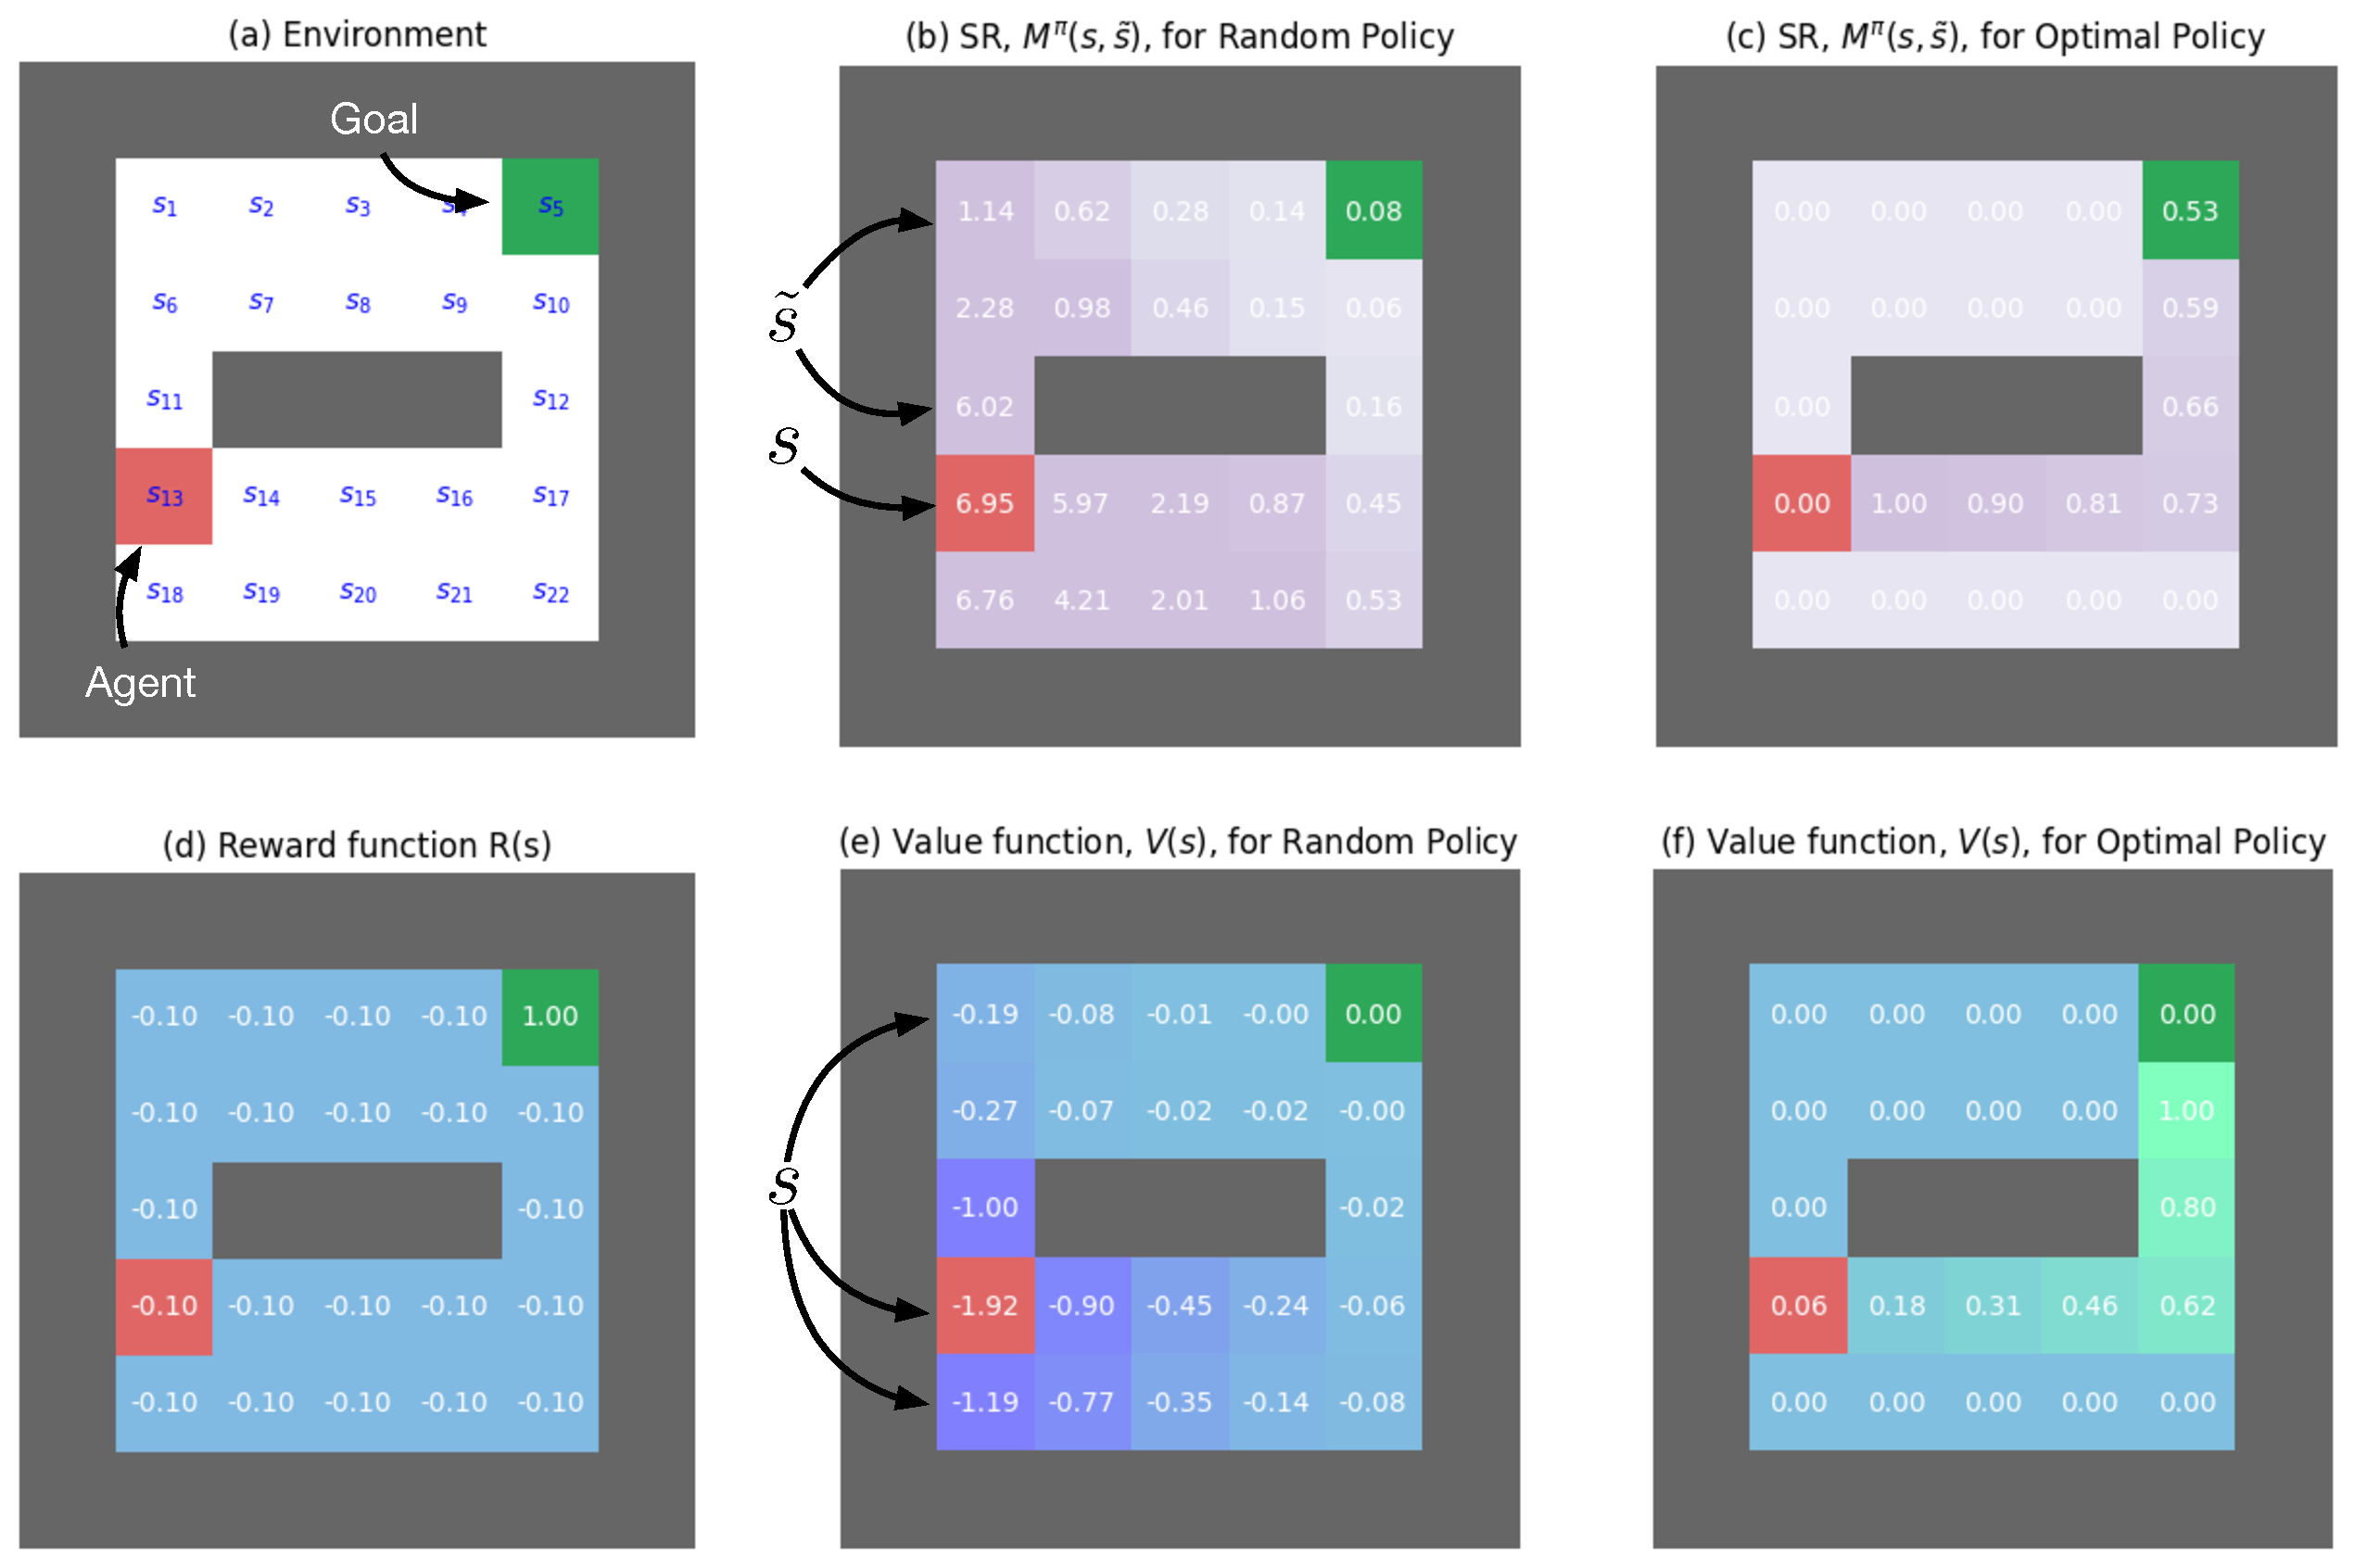
\includegraphics[height=3in]{figs/successor-rep}
\caption{
  % https://colab.sandbox.google.com/drive/1IxBmFARYobb1D3e26XzeSkTEOFxt8cxI?usp=sharing
  Illustration of successor representation for
  the 2d maze environment shown in (a) with reward
  shown in (d), which assings all states a reward of -0.1
  except for the goal state which has a reward of 1.0.
  In (b-c) we show the  SRs for a random policy and the optimal policy.
  In (e-f) we show the corresponding value functons.
%
  In (b), we see that the SR under the random policy
  assigns high state occupancy values to states which are close
  (in Manhattan distance)
  to the current state $s_{13}$
  (e.g., $M^{\pi}(s_{13}, s_{14})=5.97$)
  and low values to states that are further away
  (e.g., $M^{\pi}(s_{13}, s_{12})=0.16$).
%
  In (c), we see that the SR under the optimal policy
  assigns high state occupancy values to states which are close
  to the optimal path to the goal
  (e.g., $M^{\pi}(s_{13}, s_{14})=1.0$)
  and which fade with distance from the current state
  along that path
  (e.g., $M^{\pi}(s_{13}, s_{12})=0.66$).
  \figtaken{Figure 3 of \citep{Carvalho2024}}.
  \figthanks{Wilka Carvalho}.
  \figgen{\url{https://github.com/wcarvalho/jaxneurorl/blob/main/successor_representation.ipynb}}.
}
\label{fig:successorRep}
\end{figure}

We can also make a version of SR that depends on the action
as well as the state to get
\begin{align}
M^{\pi}(s,a,\tilde{s})
&= \expect{\sum_{t=0}^{\infty} \gamma^t \ind{s_{t+1}=\tilde{s}}
  \vert s_0=s, a_0=a, a_{1:\infty} \sim \pi} \\
&= \expect{\ind{s'=\tilde{s}} + \gamma M^{\pi}(s',a,\tilde{s})
  \vert s_0=s, a_0=a, a_{1:\infty} \sim \pi}
\end{align}
This gives rise to a TD update of the form
\begin{align}
  M^{\pi}(s,a,\tilde{s}) &\leftarrow
  M^{\pi}(s,a,\tilde{s}) + \eta 
  \underbrace{\left( \ind{s'=\tilde{s}} + \gamma M^{\pi}(s',a',\tilde{s})
     - M^{\pi}(s,a,\tilde{s}) \right)}_{\delta}
\end{align}
where $s'$ is the next state sampled from $T(s'|s,a)$
and $a'$ is the next action sampled from $\pi(s')$.
Compare this to the (on-policy) SARSA update from
\cref{eqn:rl-td-q}:
\be
Q^{\pi}(s,a) \leftarrow
Q^{\pi}(s,a) + \eta \underbrace{ \left(
  R(s') + \gamma Q^{\pi}(s',a') - Q^{\pi}(s,a) \right)}_{\delta}
\ee
However, from an SR, we can compute the state-action value function
for any reward function:
\be
Q^{R,\pi}(s,a) = \sum_{\tilde{s}} M^{\pi}(s,a,\tilde{s}) R(\tilde{s})
\ee
This can be used to improve the policy as we discuss
in \cref{sec:GPI}.

We see that the SR  representation has the computational
advantages of model-free RL (no need to do explicit planning or rollouts
in order to compute the  optimal action),
but also the flexibility of model-based RL
(we can easily change the reward function without having
to learn a new value function).
This latter property makes SR particularly well suited
to problems that use intrinsic reward (see \cref{sec:intrinsicReward}),
which often changes depending on the information state of the agent.

Unfortunately, the SR is limited in several ways:
(1) it assumes a finite, discrete state space;
(2)  it depends on a given policy.
%(3) it assumes the environment dynamics remain constant,
%even if the reward changes.
We discuss ways to overcome limitation 1 in
\cref{sec:SM},  and limitation 2 in \cref{sec:GPI}.


\subsection{Successor models}
\label{sec:SM}

In this section, we discuss the \keywordDef{successor model}
(also called a $\gamma$-model),
which is a probabilistic extension of SR
\citep{Janner2020,Eysenbach2021}.
This allows us
to generalize SR to work with continuous states and actions,
and to simulate future state trajectories.
The approach is to define the cumulant as the $k$-step conditional
distribution $C(s_{k+1}) = P(s_{k+1}=\tilde{s}|s_0=s,\pi)$,
which is the probability of being in state $\tilde{s}$
after following $\pi$ for $k$ steps starting from
state $s$. (Compare this to the SR cumulant,
which is $C(s_{k+1})=\ind{s_{k+1}=\tilde{s}}$.)
The SM is then defined as
\be
\vmu^{\pi}(\tilde{s}|s)
=(1-\gamma) \sum_{t=0}^{\infty} \gamma^t P(s_{t+1}=\tilde{s}|s_0=s)
\ee
where the $1-\gamma$ term ensures that $\vmu^{\pi}$ integrates to 1.
(Recall that $\sum_{t=0}^{\infty} \gamma^t = \frac{1}{1-\gamma}$ for $\gamma<1$.)
In the tabular setting, the SM is just the normalized SR,
since
\begin{align}
\vmu^{\pi}(\tilde{s}|s)
&=(1-\gamma) M^{\pi}(s,\tilde{s}) \\
&=(1-\gamma) \expect{\sum_{t=0}^{\infty} \gamma^t \ind{s_{t+1}=\tilde{s}}
  |s_0=s, a_{0:\infty} \sim \pi} \\
&= (1-\gamma) \sum_{t=0}^{\infty} \gamma^t P(s_{t+1}=\tilde{s}|s_0=s, \pi)
\end{align}
Thus $\vmu^{\pi}(\tilde{s}|s)$
tells us the probability that $\tilde{s}$ can be reached from $s$
within a horizon determined by $\gamma$ when  following $\pi$,
even though we don't know exactly when we will reach $\tilde{s}$.

SMs obey a Bellman-like recursion
\be
\vmu^{\pi}(\tilde{s}|s) = \expect{
  (1-\gamma) T(\tilde{s}|s,a) + \gamma \vmu^{\pi}(\tilde{s}|s')}
\ee
We can use this to perform policy evaluation by computing
\be
V^{\pi}(s) = \frac{1}{1-\gamma}
\expectQ{R(\tilde{s})}{\vmu^{\pi}(\tilde{s}|s)}
\ee

We can also define an action-conditioned SM
\begin{align}
\vmu^{\pi}(\tilde{s}|s,a)
&=(1-\gamma) \sum_{t=0}^{\infty} \gamma^t P(s_{t+1}=\tilde{s}|s_0=s,a_0=a) \\
&=(1-\gamma) T(\tilde{s}|s,a) + \gamma \expect{\vmu^{\pi}(\tilde{s}|s',a',\pi)}
\end{align}
Hence we can learn an SM using a TD update of the form
\begin{align}
  \vmu^{\pi}(\tilde{s}|s,a) &\leftarrow
  \vmu^{\pi}(\tilde{s}|s,a) + \eta 
  \underbrace{\left( (1-\gamma) T(s'|s,a)
    + \gamma \vmu^{\pi}(\tilde{s}|s',a')
    - \vmu^{\pi}(\tilde{s}|s,a) \right)}_{\delta}
  \label{eqn:SMQTD}
\end{align}
where $s'$ is the next state sampled from $T(s'|s,a)$
and $a'$ is the next action sampled from $\pi(s')$.
\eat{
Compare this to the Q-learning update
\be
Q^{\pi}(s,a) \leftarrow
Q^{\pi}(s,a) + \eta \underbrace{ \left(
  R(s') + \gamma Q^{\pi}(s',a') - Q^{\pi}(s,a) \right)}_{\delta}
\ee
}
With an SM, we can  compute the state-action value
for any reward:
\be
Q^{R,\pi}(s,a) = \frac{1}{1-\gamma}
\expectQ{R(\tilde{s})}{\vmu^{\pi}(\tilde{s}|s,a)}
\ee
This can be used to improve the policy as we discuss
in \cref{sec:GPI}.



\subsubsection{Learning SMs}

Although we can learn SMs
using the TD
update in \cref{eqn:SMQTD},
this requires evaluating
$T(s'|s,a)$ to compute the target update $\delta$,
and this one-step transition model is typically unknown.
Instead, since $\vmu^{\pi}$ is a conditional density model,
we will optimize
the cross-entropy TD loss
\citep{Janner2020}, defined as follows
\be
\loss_{\mu} = \expectQ{\log \vmu_{\vtheta}(\tilde{s}|s,a)}
     {(s,a) \sim p(s,a),
       \tilde{s} \sim (T^{\pi} \vmu^{\pi})(\cdot|s,a)}
\ee
where $(T^{\pi} \vmu^{\pi})(\cdot|s,a)$ is the Bellman
operator applied to $\vmu^{\pi}$ and then evaluated
at $(s,a)$, i.e.,
\be
(T^{\pi} \vmu^{\pi})(\tilde{s}|s,a)
=(1-\gamma) T(s'|s,a) + \gamma \sum_{s'}
T(s'|s,a) \sum_{a'} \pi(a'|s'( \vmu^{\pi}(\tilde{s}|s',a')
\ee
We can sample from this as follows:
first sample $s' \sim T(s'|s,a)$ from the environment
and then
with probability $1-\gamma$ 
set $\tilde{s}=s'$ and terminate.
Otherwise sample $a' \sim \pi(a'|s')$
and then create a bootstrap sample
from the model using $\tilde{s} \sim \vmu^{\pi}(\tilde{s}|s',a')$.

There are many possible density models we can use for
$\vmu^{\pi}$.
In \citep{Thakoor2022}, they use a VAE.
In \citep{Tomar2024}, they use
an autoregressive transformer applied
to a set of  discrete
latent tokens, which are learned using VQ-VAE or
a non-reconstructive self-supervised loss.
They call their method \keywordDef{Video Occcupancy Models}.


An alternative approach to learning SMs, that avoids fitting a normalized
density model over states, is to use contrastive learning
to estimate how likely $\tilde{s}$ is to occur
after some number of steps, given $(s,a)$,
compared to some randomly sampled negative state
\citep{Eysenbach2021C,Zheng2024contrastive}.
Although we can't sample from the resulting learned model
(we can only use it for evaluation),
we can use it to improve a policy that achieves
a target state (an approach known as
goal-conditioned policy learning,
discussed in \cref{sec:GCRL}).

\subsubsection{Jumpy models using  geometric policy composition}
\label{sec:jumpy}

In \citep{Thakoor2022}, they propose
\keywordDef{geometric policy composition} or GPC
as a way to learn a new policy by sequencing together
a set of $N$ policies, as opposed to taking $N$ primitive actions
in a row.
This can be thought of as a \keywordDef{jumpy model}, since it predicts
multiple steps into the future, instead of one step at a time
(c.f., \citep{Zhang2023jumpy}).

In more detail, in GPC, the agent picks a sequence of $n$
policies $\pi_i$ for $i=1:n$, and then samples states
according to their corresponding SMs:
starting with $(s_0,a_0)$, we sample
$s_1 \sim \vmu_{\gamma}^{\pi_1}(\cdot|s_0,a_0)$,
then $a_1 \sim \pi_1(\cdot | s_1)$,
then
$s_2 \sim \vmu_{\gamma}^{\pi_2}(\cdot|s_1,a_1)$,
etc.
This continues for $n-1$ steps.
Finally we sample $s_n \sim \vmu_{\gamma'}^{\pi_n}(\cdot|s_{n-1},a_{n-1})$,
where $\gamma' > \gamma$ represents a longer horizon SM.
The reward estimates computed along this sampled path can then
be combined to compute the value of each candidate policy sequence.


\subsection{Successor features}
\label{sec:SF}

Both SRs and SMs require defining expectations
or distributions over the entire future state vector,
which can be problematic in high dimensional spaces.
In \citep{Barreto2017} they introduced
\keywordDef{successor features}, that generalize
SRs by working with features $\vphi(s)$ instead
of primitive states. In particular, if we define
the cumulant to be
$C(s_{t+1}) = \vphi(s_{t+1})$,
we get the following definition of SF:
\be
\vpsi^{\pi,\vphi}(s) = \expect{
  \sum_{t=0}^{\infty} \gamma^t \vphi(s_{t+1}) \vert s_0=s, a_{0:\infty} \sim \pi}
\ee
We will henceforth drop the $\vphi$ superscript from the notation,
for brevity.
SFs obey a Bellman equation
\be
\vpsi(s) = \expect{\vphi(s') + \gamma \vpsi(s')}
\ee

If we assume the reward function can be written as
\be
R(s,\vw) = \vphi(s)^\trans \vw
\ee
then we can derive the value function for any reward
as follows:
\begin{align}
  V^{\pi,\vw}(s)
  &= \expect{R(s_1) + \gamma R(s_2) + \cdots \vert  s_0=s} \\
  &= \expect{\vphi(s_1)^\trans \vw + \gamma \vphi(s_2)^\trans \vw + \cdots \vert  s_0=s} \\
  &= \expect{\sum_{t=0}^{\infty} \gamma^t \vphi(s_{t+1}) \vert  s_0=s}^\trans \vw 
  = \vpsi^{\pi}(s)^\trans \vw
\end{align}


Similarly we can define an action-conditioned version of SF as
\begin{align}
\vpsi^{\pi,\vphi}(s,a) &= \expect{
  \sum_{t=0}^{\infty} \vphi(s_{t+1}) \vert s_0=s, a_0=a, a_{1:\infty} \sim \pi} \\
&= \expect{\vphi(s') + \gamma \vpsi(s',a')}
\end{align}
We can learn this using a TD rule
\be
\vpsi^{\pi}(s,a) \leftarrow
\vpsi^{\pi}(s,a) + \eta \underbrace{
  \left( \vphi(s') + \gamma \vpsi^{\pi}(s', a') - \vpsi^{\pi}(s,a) \right)}_{\delta}
\label{eqn:SFTD}
\ee
And we can use it to derive a state-action value function:
\begin{align}
  Q^{\pi,\vw}(s)
  = \vpsi^{\pi}(s,a)^\trans \vw
\end{align}
This allows us to define multiple $Q$ functions (and hence policies)
just by changing the weight vector $\vw$, as we discuss in \cref{sec:GPI}.


\subsubsection{Generalized policy improvement}
\label{sec:GPI}

So far, we have discussed how to compute the value function
for a new reward function but using the SFs
from an existing known policy.
In this section we discuss how to create a new policy
that is better than an existing set of policies,
by using \keywordDef{Generalized Policy Improvement}
or \keywordDef{GPI} \citep{Barreto2017,Barreto2020}.



\begin{figure}
\centering
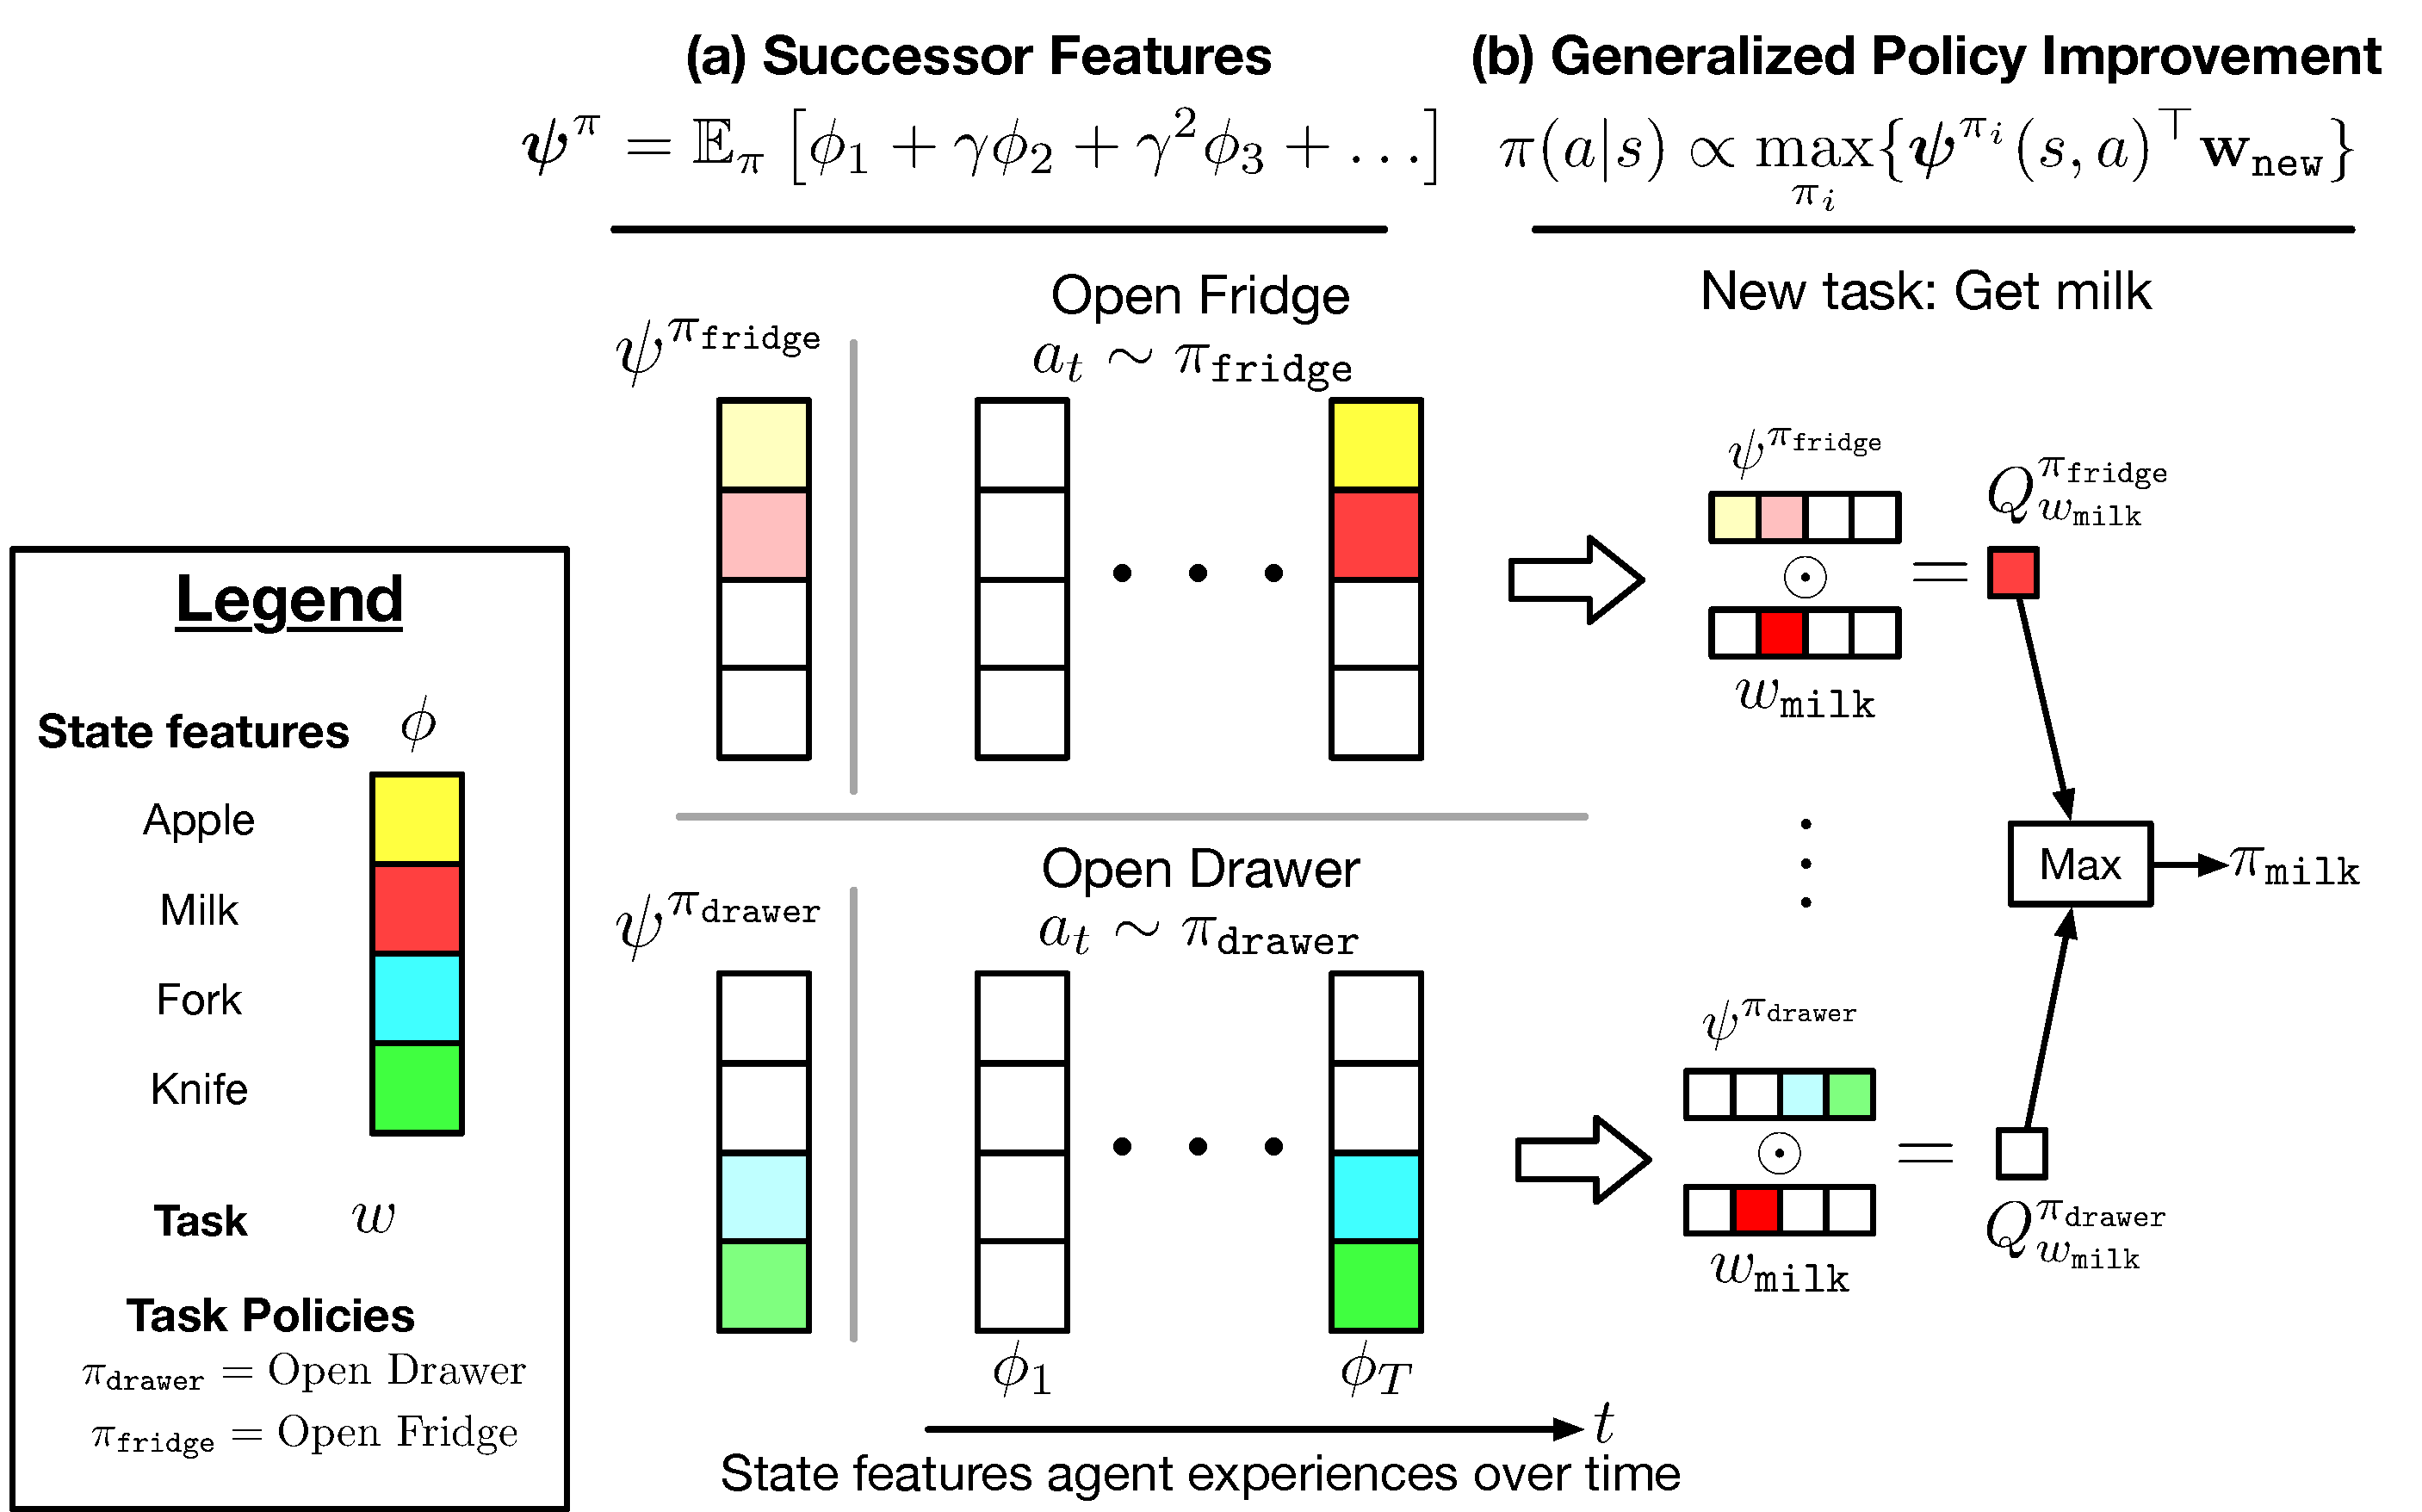
\includegraphics[height=3in]{figs/successor-features}
\caption{
  Illustration of successor features representation.
  (a)
  Here $\vphi_t=\vphi(s_t)$ is the vector of features
  for the state at time $t$, and $\vpsi^{\pi}$
  is the corresponding SF representation, which depends
  on the policy $\pi$.
  (b) Given a set of existing policies and their SFs,
  we can create a new one by specifying a desired
  weight vector $\wnew$ and taking a weighted combination
  of the existing SFs.
  \figtaken{Figure 5 of \citep{Carvalho2024}}.
    \figthanks{Wilka Carvalho}.
}
\label{fig:successorFeatures}
\end{figure}

Suppose we have learned a set of $N$ (potentially optimal)
policies $\pi_i$ and their corresponding SFs $\vpsi^{\pi_i}$
for maximizing rewards defined by $\vw_i$.
When presented with a new task $\wnew$,
we can compute a new policy using GPI as follows:
\begin{align}
  a^*(s;\wnew) &=
  \argmax_a \max_i Q^{\pi_i}(s,a,\wnew)
  =\argmax_a \max_i \vpsi^{\pi_i}(s,a)^\trans \wnew
\end{align}
If $\wnew$ is in the span of the training tasks
(i.e., there exist weights $\alpha_i$ such that $\wnew \sum_i \alpha_i \vw_i$),
then the GPI theorem states that $\pi(a|s)=\ind{a=a^*(s,\wnew)}$
will perform at least as well as any of the existing policies,
i.e., $Q^{\pi}(s,a) \geq \max_i Q^{\pi_i}(s,a)$
(c.f.,  policy improvement in \cref{sec:policyImprovement}).
See \cref{fig:successorFeatures} for an illustration.

Note that GPI is a model-free approach to computing a new policy,
based on an existing library of policies.
In \citep{Alegre2023}, they propose an extension that can also
leverage a (possibly approximate) world model to learn
better policies that can outperform the library
of existing policies by performing more decision-time search.


\subsubsection{Option keyboard}

One limitation of GPI is that it requires that the reward
function, and the resulting policy, be defined in terms of a fixed
weight vector $\wnew$, where the preference over features
is constant over time. However, for some tasks we might
want to initially avoid a feature or state and then later move
towards it.
To solve this, 
\citep{Barreto2019,Barreto2020} introduced the \keywordDef{option keyboard},
in which the weight vector for a task can be computed
dynamically in a state-dependent way, using
$\vw_s = g(s,\wnew)$.
(Options are discussed in \cref{sec:options}.)
Actions can then be chosen as follows:
\begin{align}
  a^*(s;\wnew) &=
    \argmax_a \max_i \vpsi^{\pi_i}(s,a)^\trans \vw_s
\end{align}
Thus the policy $\pi_i$ that is chosen  depends
in the current state. Thus $\vw_s$ induces a set of policies
that are active for a period of time, similar to playing
a chord on a piano.

%\subsubsection{Discovering cumulants}




\subsubsection{Learning SFs}

A key question when using SFs is how to learn the cumulants
or state-features
$\vphi(s)$.
Various approaches have been suggested,
including leveraging meta-gradients \citep{Veeriah2019},
image reconstruction \citep{Machado2018eigen},
and
maximizing the mutual information between task encodings
and the cumulants that an agent experiences when pursuing that task
\citep{Hansen2019}.
The cumulants are encouraged to satisfies the linear reward
constraint by minimizing
\be
\loss_r = ||r-\vphi_{\vtheta}(s)^\trans \vw||_2^2
\ee

Once the cumulant function is known,
we have to learn the corresponding SF.
The standard approach learns a different SF for every policy,
which is limiting. In \citep{Borsa2019} they introduced
\keywordDef{Universal Successor Feature Approximators}
which takes an input a policy encoding $\vz_{\vw}$,
representing a policy $\pi_{\vw}$ (typically we set $\vz_{\vw}=\vw$).
We then define
\be
\vpsi^{\pi_{\vw}}(s,a) = \vpsi_{\vtheta}(s,a,\vz_{\vw})
\ee
The GPI update then becomes
\be
a^*(s;\wnew) = \argmax_a \max_{\vz_{\vw}} \vpsi_{\vtheta}(s,a,\vz_{\vw})^\trans \wnew
\ee
so we replace the discrete max over a finite number of policies
with a continuous optimization problem (to be solved per state).

If we want to learn the policies and SFs at the same time,
we can optimize the following losses in parallel:
\begin{align}
  \loss_Q &= ||\vpsi_{\vtheta}(s,a,\vz_w)^\trans \vw - \vy_Q||,
  \;
  \vy_Q = R(s';\vw) + \gamma \vpsi_{\vtheta}(s',a^*,\vz_w)^\trans \vw
  \label{eqn:LQ} \\
  \loss_{\vpsi} &= ||\vpsi_{\vtheta}(s,a,\vz_{\vw}) - \vy_{\vpsi}||,
  \;
  \vy_{\vpsi} = \vphi(s') + \gamma \vpsi_{\vtheta}(s',a^*,\vz_{\vw})
\end{align}
where $a^* = \argmax_{a'} \vpsi_{\vtheta}(s', a', \vz_{\vw})^\trans \vw$.
The first equation is standard Q learning loss,
and the second is the TD update rule
in \cref{eqn:SFTD} for the SF.
In \citep{Carvalho2023}, they present the
\keywordDef{Successor Features Keyboard},
that can learn the policy,
the SFs 
and the task encoding $\vz_{\vw}$,
all simultaneously.
They also suggest replacing the squared error regression
loss in \cref{eqn:LQ} with a cross-entropy loss,
where each dimension of the SF is now a
discrete probability distribution
over $M$ possible values of the corresponding feature.
(c.f. \cref{sec:classifRL}).


\subsubsection{Choosing the tasks}

A key advantage of SFs is that they provide a way
to compute a value function and policy for any given reward,
as specified by a task-specific weight vector $\vw$.
But how do we choose these tasks?
In \citep{Hansen2019} they sample $\vw$ from a distribution
at the start of each task, to encourage the agent
to learn to explore different parts of the state space
(as specified by the feature function $\vphi$).
In \citep{Liu2021} they extend this by adding an intrinsic
reward that favors exploring parts of the state space
that are surprising (i.e., which induce high entropy),
c.f., \cref{sec:intrinsicReward}.
In \citep{Farebrother2023}, they introduce
\keywordDef{proto-value networks},
which is a way to define auxiliary tasks based on  successor
measures.

\eat{
\subsection{Forwards-backwards representations: TODO}
\label{sec:FB}

\citep{Touati2021,Touati2023}
}


%%%%%%%%%%%


\eat{
\subsection{Predictive state representations}
\label{sec:PSR}

An alternative to working with belief states
is to  marginalize out the POMDP
latent state $z_t$,
to derive a set of predictions over future observables $\vo_{t+1:T}$
as a function of the past history of observables, $\vh_t$,
and future actions, $\va_{t+1:T}$.
This can then become a learning  target for a model, that is trained
to directly
predict  future observations, without explicitly invoking the concept
of latent state.
This is called a \keywordDef{predictive state representation}
or \keywordDef{PSR} \citep{PSR}.
This is related to the idea of
\keywordDef{observable operator models}
\citep{Jaeger2000}.
See also \cref{sec:SR} where we discuss successor representations.
%However, it is not clear which features of the future observables
%are worth modeling.
%(GVFs, discussed in \cref{sec:GVF}, share the same problem.)
}


\eat{
\subsection{General value functions}
\label{sec:GVF}

So far we have mainly been focused on predicting the sum of expected
discounted future rewards, i.e., the value function.
But the reward is just one possible signal of interest we can extract from the environment.
We can generalize this by considering a \keywordDef{cumulant}
$C_t \in \real$, which is some scalar of interest derived from the observation
(e.g., did a loud bang just occur? is there a tree visible in the image?).
We then define the \keywordDef{general value function} or \keywordDef{GVF}
as follows \citep{GVF}:
\be
V_{\pi,\gamma,C}(s) = \expect{
  \sum_{k=t}^{\infty} \left(\prod_{i=t+1}^k \gamma(S_i) \right)
  C_{k+1} \vert S_t=s, A_{t:\infty} \sim \pi}
\ee
where $1-\gamma(s)$ is the probability of terminating in state $s$.
If we set $C(s)=R(s)$ and $\gamma(s)=\gamma$, we recover the value function.
But we can use the GVF to predict the probability of
other \keywordDef{auxiliary tasks}, such as the occurence of a loud bang;
and unlike a standard one-step predictive model,
we don't need to know exactly when the event will occur.
(See also \citep{Ring2021}.)

By training a model to compute GVFs for multiple related cumulants,
we can  learned a useful state representation more efficiently than just
learning from the reward by itself, while still avoiding the need
to reconstruct the entire observation.
Thus this is a form of non-generative world model,
as discussed in \cref{sec:MBRLnongen}.
The benefits of this kind of approach were shown in
\citep{Jaderberg2017iclr}.


Note that training GVFs using some kind of TD learning
is inherently an off-policy learning problem, since the data is being
collected by a policy to maximize reward, but the other cumulants
are just being predicted, not maximized.
Since the GVF is typically a neural network with multiple output heads,
we need to tackle the \keyword{deadly triad}, which we discussed in 
\cref{sec:deadlyTriad}.
One approach is to use gradient TD methods, which are provably convergent.
This has been applied to GVF learning in \citep{Xu2022GVF}.
However, the question of which cumulants are worth learning is still open.
}


%\chapter{Other topics in RL}
\label{sec:rl-other}

In this section, we briefly mention some other important topics in RL.
%This summary is based in part on \citep[Ch.17]{Suttonv2}.


\section{Distributional RL}
\label{sec:distributional}

% engression

The \keywordDef{distributional RL} approach
of \citep{Bellemare2017,BellemareBook},
predicts the distribution of (discounted) returns,
not just the expected return.
More precisely, let $Z^{\pi} = \sum_{t=0}^T \gamma^t r_t$ be a random variable
representing the reward-to-go.
The standard value function is defined to compute the expectation
of this variable: $V^{\pi}(s) = \expect{Z^{\pi}|s_0=s}$.
In DRL, we instead attempt to learn the full distribution,
$p(Z^{\pi}|s_0=s)$.
For a general review of distributional regression,
see \citep{Kneib2023}.
Below  we briefly mention a few algorithms in this class
that have been explored in the context of RL.


\subsection{Quantile regression methods}
\label{sec:QRDQN}

An alternative to predicting a full distribution
is to predict a fixed set of quantiles.
This is called quantile regression,
and has been used with DQN in
\citep{Dabney2017} to get \keywordDef{QR-DQN},
and with SAC in \citep{Wurman2022}
to get \keywordDef{QR-SAC}.
(The latter  was used in Sony's \keywordDef{GTSophy}
Gran Turismo AI racing agent.)

% quantiles may cross

\eat{
\footnote{
%
Interestingly, the original DQN paper did not
learn to predict the mean of the Q function.
since it was not trained with quadratic loss.
Instead it was trained with Huber loss,
which is quadratic if the residual error is less than 1,
and otherwise is a linear function.
Hence the gradient is clipped to be between
-1 and 1.
See \url{https://openai.com/index/openai-baselines-dqn/}
for a discussion.
}
}




\subsection{Replacing regression with classification}
\label{sec:classifRL}
\label{sec:C51}
\label{sec:catDQN}



\begin{figure}
\centering
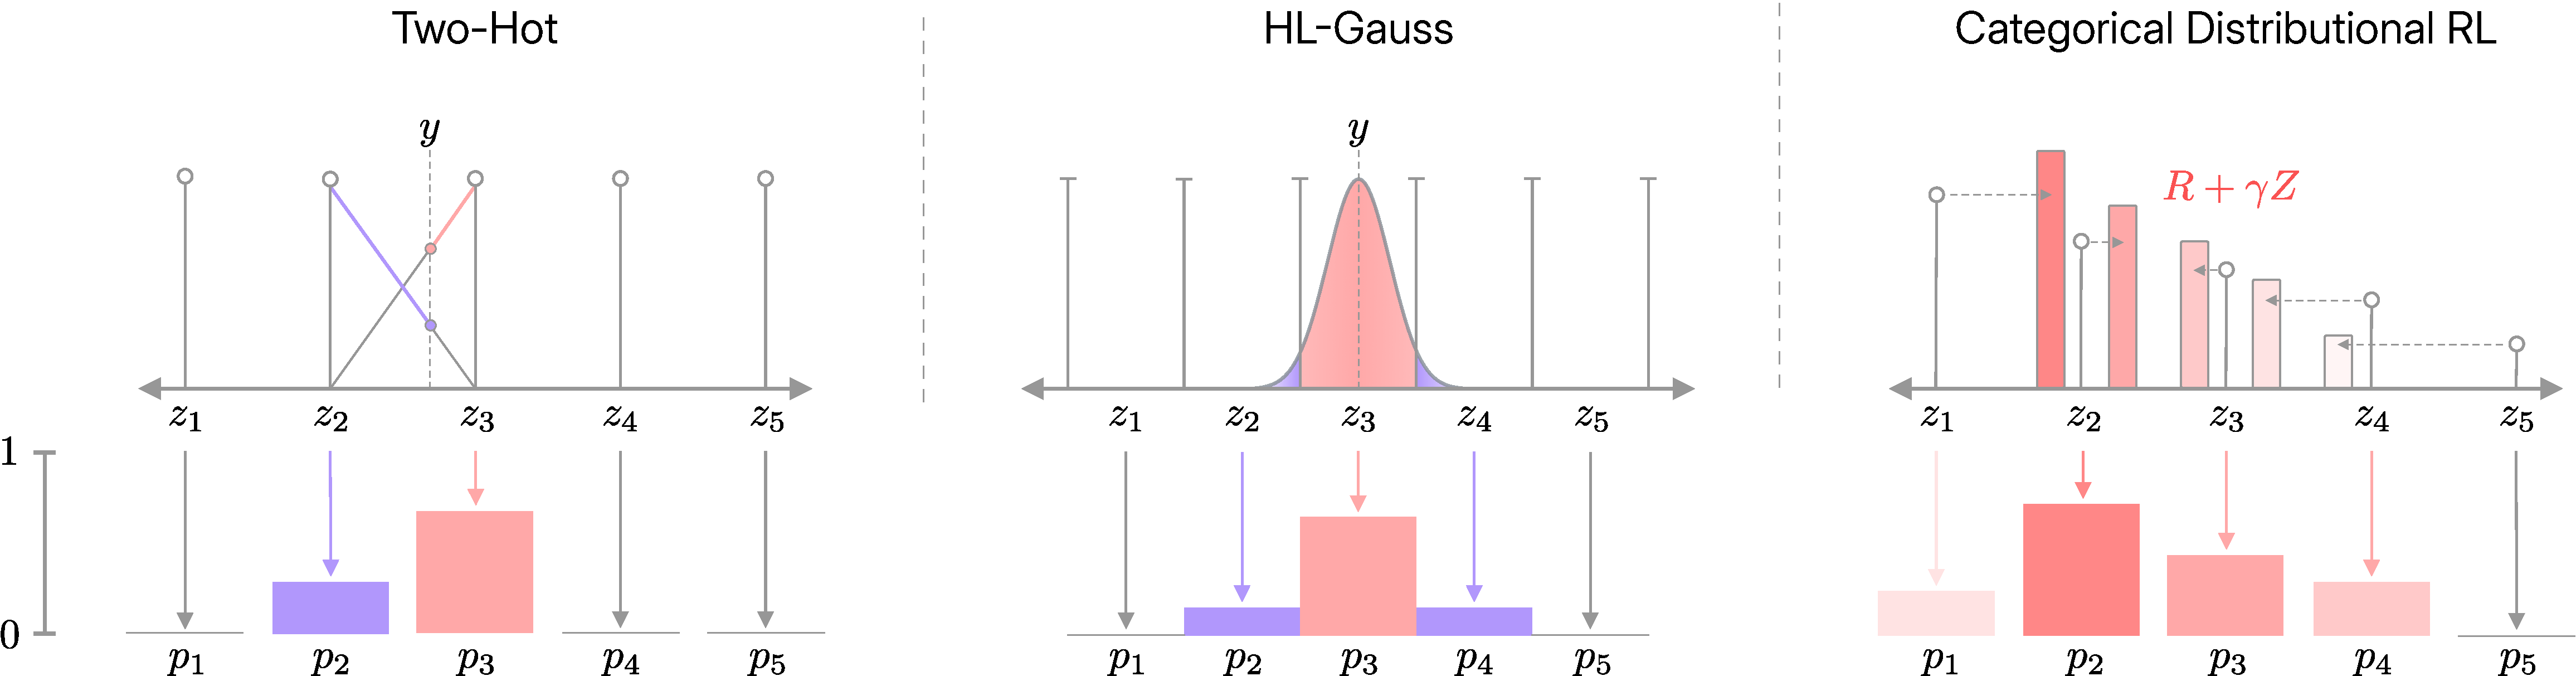
\includegraphics[height=1.5in]{figs/twoHot.pdf}
\caption{
  Illustration of how to encode a scalar target $y$
  or distributional target $Z$
using a categorical distribution.
\figtaken{Figure 1 of \citep{Farebrother2024}}.
\figthanks{Jesse Farebrother}.
}
\label{fig:twoHot}
\end{figure}


An alternative to quantile regression
is to approximate the distribution over returns
using a histogram, and then fit it
using cross entropy loss (see \cref{fig:twoHot}).
This approach was first suggested in \citep{Bellemare2017},
who called it  \keywordDef{categorical DQN}.
(In their paper, they use 51 discrete categories (atoms),
giving rise to the name \keywordDef{C51}.) 

An even simpler approach is to replace the distributional
target with the standard scalar target (representing the mean),
and then discretize this target
and use cross entropy loss instead of squared error.\footnote{
%
Technically speaking, this is no longer a distributional RL method,
since the prediction target is the mean,
but the mechanism for predicting the mean leverages a distribution,
for robustness and ease of optimization.
}
Unfortunately, this encoding is lossy.
In  \citep{Schrittwieser2020}, they
proposed the \keywordDef{two-hot} transform,
that is a lossless encoding of the target based on putting
appropriate weight on the nearest two bins (see \cref{fig:twoHot}).
In \citep{Imani2018}, they proposed the
\keywordDef{HL-Gauss} histogram loss,
that convolves the target value $y$ with a Gaussian,
and then discretizes the resulting continuous distribution.
This is  more symetric than two-hot encoding, as shown in \cref{fig:twoHot}.
Regardless of how the discrete target is chosen,
predictions are made using
$\hat{y}(s;\vtheta) = \sum_k p_k(s) b_k$,
where $p_k(s)$ is the probability of bin $k$,
and $b_k$ is the bin center.

In \citep{Farebrother2024}, they show that 
the HL-Gauss trick  works much better than
MSE,  two-hot and C51 across a variety of problems
(both offline and online),
especially  when they scale to large networks.
They conjecture that the reason it beats MSE
is that cross entropy is more robust to noisy targets
(e.g., due to stochasticity) and nonstationary targets.
They also conjecture  that the reason HL works better than two-hot
is that HL is closer to ordinal regression, and reduces overfitting
by having a softer (more entropic) target distribution
(similiar to label smoothing in classification problems).



\section{Reward functions}
\label{sec:reward}

Sequential decision making relies on the
 user to define the reward function in order to
 encourage the agent to exhibit some desired behavior.
In this section, we discuss this crucial aspect of the problem.
%However, sometimes we want or need to learn the reward function,
%as we discuss below.


\subsection{Reward hacking}
\label{sec:rewardHacking}
\label{sec:hacking}

In some cases, the reward function may be misspecified, so even though the agent may
maximize the reward, this might turn out not to be what the user desired.
For example, suppose the user rewards the agent for making as many
paper clips as possible.
An optimal agent may convert the whole world into a paper clip factory,
because the user forgot to specify various constraints, such as not
killing people or not destroying the environment.
In the \keywordDef{AI alignment} community,
this example is known as  the \keywordDef{paperclip maximizer problem},
and is due to Nick Bostrom \citep{Bostrom2016}.
(See e.g., \url{https://openai.com/index/faulty-reward-functions/} for some examples
that have occurred in practice.)
This is an example of a more general problem
known as
%\keywordDef{Goodhart's law} or
\keywordDef{reward hacking}
\citep{Skalse2022}.
For a potential solution, based on the assistance game paradigm,
see \cref{sec:assistance}.


\eat{
For example, a rat which can electrically stimulate its dopamine
center by pressing a lever, will press the lever indefinitely,
until it starves to death \citep{Bennett2023}; this is known as
\keywordDef{wire heading}, and illustrates
the dangers of changing the reward function.
}

\subsection{Sparse reward}

Even if the reward function is correct, optimizing it is not always easy.
In particular, many problems suffer from \keywordDef{sparse reward},
in which $R(s,a)=0$ for almost all states and actions, so the agent
only every gets feedback (either positive or negative) on the rare occasions
when it achieves some unknown goal.
This requires \keywordDef{deep exploration}
\citep{Osband2019}
to find the rewarding states.
One approach to this is use to use PSRL (\cref{sec:PSRL}).
However, various other heuristics have been developed,
some of which we discuss below.


\subsection{Reward shaping}
\label{sec:rewardShaping}

In  \keywordDef{reward shaping},
we add prior knowledge about what we believe good states should look like,
as a way to combat the difficulties of learning from sparse reward.
That is, we define a new reward function $r' = r + F$,
where $F$ is called the shaping function.
In general, this can affect the optimal policy.
For example, if a soccer playing agent is ``artificially''
rewarded for making contact with the ball,
it might learn to repeatedly touch and untouch the ball
(toggling between $s$ and $s'$), rather than
trying to win the original game.
But in \citep{Ng99},
the prove that if the shaping function has the form
\be
F(s,a,s') = \gamma \Phi(s') - \Phi(s)
\ee
where $\Phi: \calS \ra \real$
is a \keywordDef{potential function},
then we can guarantee that the sum of shaped rewards
will match the sum of original rewards plus a constant.
This is called \keywordDef{Potential-Based Reward Shaping}.

In \citep{Wiewiora2003}, they prove that (in the tabular case)
this approach
is equivalent to initializing the value function
to $V(s)=\Phi(s)$.
%In \citep{Wiewiora2003aaai}, 
In \citep{Tessler2019},
they propose
an extension called potential-based advice,
where they show that a potential of the form
$F(s,a,s',a') = \gamma \Phi(s',a') - \Phi(s,a)$
is also valid (and more expressive).
In \citep{Hu2020}, they introduce a reward shaping function $z$
which can be used to down-weight or up-weight the
shaping function:
\be
r'(s,a) = r(s,a) + z_{\phi}(s,a) F(s,a)
\ee
They use bilevel optimization to optimize $\phi$
wrt the original task performance.


% https://gibberblot.github.io/rl-notes/single-agent/reward-shaping.html#potential-based-reward-shaping
%



\subsection{Intrinsic reward}
\label{sec:intrinsicReward}
\label{sec:intrinsic}

When the extrinsic reward is sparse,
it can be useful to (also) reward the agent for solving
``generally useful'' tasks,
such as learning about the world.
This is called \keywordDef{intrinsically motivated RL}
\citep{Aubret2023,Linke2019,Amin2021,Yuan2022,Yuan2024,Colas2022}.
It can be thought of as a special case of reward shaping,
where the shaping function is dynamically computed.

We can classify these methods into two main types:
\keywordDef{knowledge-based intrinsic motivation},
or \keywordDef{artificial curiosity},
where the agent is
rewarded for learning about its environment;
and  \keywordDef{competence-based intrinsic motivation},
where the agent is rewarded for achieving novel goals
or mastering new skills.

\subsubsection{Knowledge-based intrinsic motivation}

One simple approach to knowledge-based intrinsic motivation
is to add to the extrinsic reward
an intrinsic \keywordDef{exploration bonus}
$R_t^i(s_t)$,
which is high when the agent visits novel states.
For tabular environments, we can just count the number of visits to each state,
$N_t(s)$, and define $R_t^i(s) = 1/N_t(s)$ or
$R_t^i(s) = 1/\sqrt{N_t(s)}$, which is similar to the UCB
heuristic used in bandits (see \cref{sec:UCB}).
We can  extend exploration bonuses  to high dimensional states (e.g. images)
using density models \citep{Bellemare2016}.
Alternatively, \citep{Machado2020} propose to use the $\ell_1$
norm of the successor feature (\cref{sec:SF}) representation
as an alternative to the visitation count, giving rise
to an intrinsic reward of the form
$R^i(s) = 1/||\vpsi^{\pi}(s)||_1$.
Recently \citep{Yu2023} extended this to combine
SFs with {\em predecessor} representations,
which encode retrospective information about the previous state
(c.f., inverse dynamics models, mentioned below).
This encourages exploration towards bottleneck states.

Another approach
is the \keywordDef{Random Network Distillation} or \keywordDef{RND}
method of \citep{Burda2018}.
This uses a fixed random neural network feature extractor
$\vz_t=f(\vs_t;\vtheta^*)$ to define a target,
and then trains a predictor $\hat{\vz}_t=f(\vs_t;\hat{\vtheta}_t)$
to predict these targets.
If $\vs_t$ is similar to previously seen states,
then the trained model will have low prediction error.
We can thus define the intrinsic reward as proportional
to the squared error $||\hat{\vz}_t - \vz_t||_2^2$.
%In  \citep{Burda2018}, they show that this metric
%is related to the predictive uncertainty
%of a deep ensemble with a random prior
%\cref{sec:rndPrior}.
The \keywordDef{BYOL-Explore} method of
\citep{Guo2022} goes beyond RND by learning
the target representation (for the next state),
rather than using a fixed random projection,
but is still based on prediction error.


\eat{
The value function now has two output heads,
one to predict the sum of extrinsic rewards,
and another to predict the sum of intrinsic rewards;
the latter can change over time as the agent learns.
The overall value is the sum of these two heads,
similar to the reward shaping term
$V(s;\vw) = V^e(s;\vw) + V^i(s;\vw')$ in \cref{sec:rewardShaping}.

The RND method has given good results on Atari games
with sparse reward, such as \keyword{Montezuma's revenge}.
as well as some continuous control problems
\citep{Laskin2021}.
}

We can also define an intrinsic reward in terms
of the information theoretic \keywordDef{surprise}
of the next state given the current one:
\be
R(\vs,\va,\vs') = -\log q(\vs'|\vs,\va)
\ee
This is the same as methods based on
rewarding states for prediction error.
Unfortunately such methods
can suffer from 
the \keywordDef{noisy TV problem}
(also called a \keywordDef{stochastic trap}),
in which an agent is attracted to states 
which are intrinsically to predict.
To see this, note that by averaging
over future states we see that the above reward reduces to
\be
R(\vs,\va) = -\expectQ{\log q(\vs'|\vs,\va)}{p^*(\vs'|\vs,\va)}
= \crossentropy(p^*, q)
\ee
where $p^*$ is the true model and $q$ is the learned dynamics model,
and $\crossentropy$ is the cros -entropy.
As we learn the optimal model, $q=p^*$,
this reduces to the conditional
entropy of the predictive distribution,
which can be non-zero for inherently unpredictable states.

To help filter out such random noise,
\citep{Pathak2017} proposes an
\keywordDef{Intrinsic Curiosity Module}.
This first learns  an \keywordDef{inverse dynamics model}
of the form $a = f(\vs,\vs')$, which tries
to predict which action was used, given
that the agent was in $\vs$ and is now in $\vs'$.
The classifier has the form
$\softmax(g(\phi(\vs), \phi(s'), a))$,
where $\vz=\phi(\vs)$ is  a representation function
that focuses  on parts of the state that the agent can control.
Then the agent learns a forwards dynamics model
in $\vz$-space.
Finally it defines the intrinsic reward as
\be
R(\vs,\va,\vs') = -\log q(\phi(\vs')|\phi(\vs),a)
\ee
Thus the agent is rewarded for visiting states that lead
to unpredictable consequences,
where the difference in outcomes is measured
in a (hopefully more meaningful) latent space.

Another solution  is to replace the cross entropy
with the KL divergence,
$R(\vs,\va) = \KL(p||q) = \crossentropy(p,q) - \entropy(p)$,
which goes to zero once the learned model matches the true model,
even for unpredictable states.
This has the desired effect of encouraging exploration towards states
which have epistemic uncertainty (reducible noise)
but not aleatoric uncertainty (irreducible noise)
\citep{Mavor-Parker2022}.
The \keywordDef{BYOL-Hindsight} method of \citep{Jarrett2023}
is one recent approach that attempts to use
the $R(\vs,\va) = \KL(p||q)$ objective.
Unfortunately, computing the $\KL(p||q)$ term is much harder
than the usual variational objective of $\KL(q||p)$.
A related idea,
proposed in the RL context by \citep{Schmidhuber2010},
is to use the \keywordDef{information gain} as a reward.
This is defined as
$R_t(\vs_t,\va_t)=\KL(q(\vs_t|\vh_t,\va_t,\vtheta_t)
|| q(\vs_t|\vh_t,\va_t,\vtheta_{t-1})$,
where $\vh_t$ is the history of past observations,
and $\vtheta_t=\text{update}(\vtheta_{t-1}, \vh_t, \va_t, \vs_t)$
are the new model parameters.
This is closely related to the BALD (Bayesian Active Learning by Disagreement)
criterion
\citep{Houlsby2011,Kirsch2019},  and has the advantage
of being  easier to compute, since it is does not reference
the true distribution $p$.
%https://people.idsia.ch/~juergen/artificial-curiosity-since-1990.html
%https://ae-foster.github.io/posts/2022/04/27/bed-bald.html



%See also e.g., \citep{Amin2021,Yuan2022} for a recent survey other intrinsic reward methods.

\subsubsection{Goal-based intrinsic motivation}
%\subsection{Go Explore: TODO}
\label{sec:goExplore}



We will discuss goal-conditioned RL
in \cref{sec:GCRL}. If the agent creates its own goals,
then it provides a way to explore the environment.
The question of when and how an agent to switch to pursuing
a new goal is studied in \citep{Pislar2022}
(see also \citep{Bagaria2023}).
Some other key work in this space includes
the \keywordDef{scheduled auxiliary control}
method of \citep{Riedmiller2018},
and
the \keywordDef{Go Explore} algorithm in 
\citep{Ecoffet2019,Ecoffet2021}
and its recent LLM extension \citep{Lu2024go}.



\eat{
\subsection{Meta-learning the reward function}
\label{sec:rewardMeta}

It may be possible to learn the reward function
using  \keywordDef{bilevel optimization problem},
where the outerloop searches over reward functions,
and the inner loop searches over policies that maximize the given reward.
The value returned by the inner loop is the score which is maximized by the outer loop.
This is analogous to evolution, which searches 
over reward functions, such as the desire for food and sex,
which are then optimized by the agent using RL.
Evolution's goal is to maximize the evolutionary fitness of each agent,
which cannot be directly measured by the agent itself,
but can be estimated at a population level.
See also \cref{sec:LLMreward}.
}



\section{Hierarchical RL}
\label{sec:HRL}

%https://thegradient.pub/the-promise-of-hierarchical-reinforcement-learning/
%https://x.com/RichardSSutton/status/1813987506200957103
%https://github.com/Jinjiarui/hrl-papers

So far we have focused on MDPs that work at a single time scale.
However, this is very limiting.
For example, imagine planning a trip from San Francisco to New York:
we need to choose high level actions first, such as which airline to fly,
and then medium level actions, such as how to get to the airport,
followed by low level actions, such as motor commands.
Thus we need to consider actions that operate multiple levels
of \keywordDef{temporal abstraction}.
This is called \keywordDef{hierarchical RL} or \keywordDef{HRL}.
This is a big and important topic,
and we only brief mention a few key ideas and methods.
Our summary is based in part on 
\citep{Pateria2022}.
(See also \cref{sec:beyond} where we discuss multi-step
predictive models; by contrast, in this section we focus
on model-free methods.)
% Hutsebaut-Buysse2022,

\subsection{Feudal (goal-conditioned) HRL}
\label{sec:feudal}
\label{sec:GCRL}

\begin{figure}
\centering
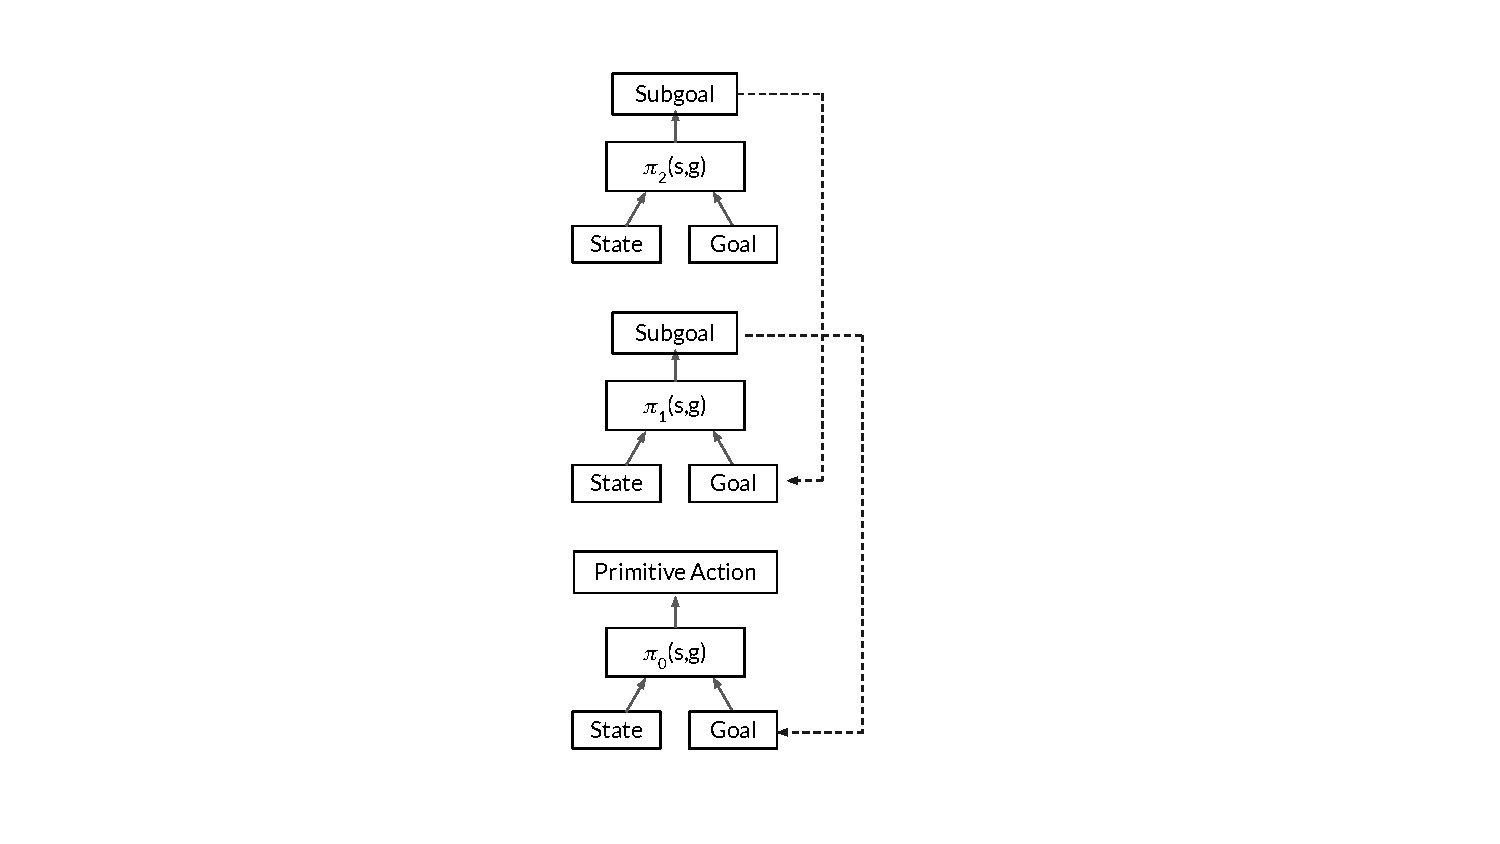
\includegraphics[height=2.5in]{figs/Goal_Cond_HRL_Architecture.pdf}
\caption{
  Illustration of a 3 level hierarchical goal-conditioned controller.
\figtaken{\url{http://bigai.cs.brown.edu/2019/09/03/hac.html}}.
\figthanks{Andrew Levy}.
}
\label{fig:HAC}
\end{figure}

In this section, we discuss an approach to HRL known as
\keywordDef{feudal RL} \citep{Dayan1992}. Here the action
space of the higher level policy consists of \keywordDef{subgoals}
that are passed down to the lower level policy.
See \cref{fig:HAC} for an illustration.
The lower level policy learns a \keywordDef{universal policy}
$\pi(a|s,g)$, where $g$ is the goal passed into it
\citep{Schaul2015}.
This policy
optimizes an MDP in which the reward is define as $R(s,a|g)=1$
iff the goal state is achieved,
i.e., $R(s,a|s) = \ind{s=g}$.
(We can also define a dense reward signal using
some state abstraction function $\phi$,
by definining $R(s,a|g)=\text{sim}(\phi(s), \phi(g))$
for some similarity metric.)
This approach to RL is known as
\keywordDef{goal-conditioned RL} \citep{Liu2022GCL}.
%The set of goals can be manually defined or discovered,
%as we discuss below.


\subsubsection{Hindsight Experience Relabeling (HER)}
\label{sec:HER}


In this section, we discuss an approach to efficiently learning
goal-conditioned  policies,
in the special case where
the set of goal states
$\calG$ is the same as the set of original states $\calS$.
We will extend this to the hierarchical case below.

The basic idea is as follows.
We collect various trajectores  in the environment,
from a starting state $s_0$ to some terminal state $s_T$,
and then define the goal of each trajectory as being $g=s_T$;
this trajectory then serves as a demonstration
of how to achieve this goal.
This is called \keywordDef{hindsight experience relabeling}
or \keywordDef{HER} \citep{HER}.
This can be used to relabel the trajectories stored in the replay buffer.
That is, if we have $(s,a,R(s|g),s',g)$ tuples, we replace them with
$(s,a,R(s|g'),g')$ where $g'=s_T$.
We can then use any off-policy RL method to learn $\pi(a|s,g)$.
In \citep{Eysenbach2020}, they show that HER can be viewed as a special
case of maximum-entropy inverse RL,
since it is estimating the reward for which the corresponding
trajectory was optimal.

\subsubsection{Hierarchical HER}
\label{sec:HAC}
\label{sec:HIRO}

We can leverage HER to learn a hierarchical controller
in several ways. In \citep{Nachum2018}
they propose \keywordDef{HIRO}
(Hierarchical Reinforcement Learning with Off-policy Correction)
as a way to train a two-level controller.
(For a two-level controller, the top level is often
called the \keywordDef{manager}, and the low level the \keywordDef{worker}.)
The data for the manager are transition tuples
of the form $(s_t, g_t, \sum r_{t:t+c}, s_{t+c})$,
where $c$ is the time taken for the worker to
reach the goal (or some maximum time),
and $r_t$ is the main task reward function at step $t$.
The data for the worker are transition tuples of the form
$(s_{t+i}, g_t, a_{t+i}, r_{t+i}^{g_t}, s_{t+i+1})$
for $i=0:c$, where $r_t^{g}$ is the reward
wrt reaching goal $g$.
This data can be used to train the two policies.
However, if the worker fails to achieve the goal
in the given time limit,
all the rewards will be 0, and no learning will take place.
To combat this,
if the worker does not achieve $g_t$
after $c$ timesteps, the subgoal is relabeled
in the transition data with another subgoal $g_t'$
which is sampled from $p(g|\tau)$,
where $\tau$ is the observed trajectory.
Thus both policies treat $g_t'$ as the goal in hindsight,
so they can use the actually collected data for training


%Unfortunately, training all levels of the hierarchy at the same time
%can be unstable.
The \keywordDef{hierarchical actor critic} (HAC) method
of \citep{Levy2018} is a simpler version of HIRO that can be extended
to multiple levels of hierarchy,
where the lowest level corresponds to primitive actions
(see \cref{fig:HAC}).
In the HAC approach, the output subgoal in the higher level data,
and the input subgoal in the lower-level data,
are replaced with the actual state that was achieved
in hindsight. This allows
the training of  each level of the
hierarchy independently of the lower levels,
by assuming  the lower level policies are already optimal
(since they achieved the specified goal).
As a result, the distribution of
$(s,a,s')$ tuples experienced by a higher level
will be stable,  providing a  stationary learning target.
By contrast, if all policies are learned simultaneously,
the distribution becomes \keywordDef{non-stationary},
which makes learning harder.
For more details, see the paper,
or the corresponding blog post (with animations)
at  \url{http://bigai.cs.brown.edu/2019/09/03/hac.html}.
%(Note that \citep{McClinton2021} combines HAC
%with intrinsic reward (\cref{sec:intrinsic})
%to improve exploration.)


\subsubsection{Learning the subgoal space}

In the previous approaches, the subgoals are defined
in terms of the states that were achieved at the end
of each trajectory, $g'=s_T$. This can be generalized
by using a state abstraction function to get
$g'=\phi(s_T)$.
The methods in \cref{sec:HIRO})
assumed that $\phi$ was manually
specified.
We now mention some ways to learn $\phi$.

In \citep{Vezhnevets2017}, they present
\keywordDef{Feudal Networks} for learning a two level hierarchy.
The manager samples subgoals in a learned latent subgoal space.
The worker uses distance to this subgoal as a reward,
and is trained in the usual way.
The manager uses the ``transition gradient'' as a reward,
which is derived from the task reward as well as the
distance between the subgoal and the actual state transition
made by the worker. This reward signal is used to learn
the manager policy and the latent subgoal space.

Feudal networks do not guarantee that the learned subgoal
space will result in optimal behavior.
In \citep{Nachum2019}, they present
a method to optimize the policy and $\phi$ function
so as to minimize a bound on the suboptimality of the hierarchical
policy.
This approach is combined with HIRO
(\cref{sec:HIRO}) to tackle the non-stationarity issue.



\subsection{Options}
\label{sec:options}

The feudal approach to HRL is somewhat limited,
since not all subroutines or skills can be defined in terms
of reaching a goal state (even if it is a partially
specified one, such as being in a desired location
but without specifying the velocity).
For example, consider the skill of
``driving in a circle'', or ``finding food''.
The \keywordDef{options} framework  is a
more general framework for HRL first proposed in
\citep{options}.
We discuss this below.

\subsubsection{Definitions}

An option $\omega=(I,\pi,\beta)$ is a tuple consisting of:
the \keywordDef{initiation set} $I_{\omega} \subset S$,
which is a subset of states that this option can start from
(also called the \keywordDef{affordances} of  each state
\citep{Khetarpal2020});
the \keywordDef{subpolicy} $\pi_{\omega}(a|s) \in [0,1]$;
and the \keywordDef{termination condition}
$\beta_{\omega}(s) \in [0,1]$,
which gives the probability of finishing in state $s$.
(This induces a geometric distribution over option durations,
which we denote by $\tau \sim \beta_{\omega}$.)
The set of all options is denoted $\Omega$.

To execute an option at step $t$ entails choosing an action using
$a_t = \pi_{\omega}(s_t)$ and then deciding whether
to terminate at step $t+1$ with probability
$1-\beta_{\omega}(s_{t+1})$ or to continue following the option at step $t+1$.
(This is an example of a \keywordDef{semi-Markov decision process}
\citep{Puterman94}.)
If we define $\pi_{\omega}(s)=a$ and $\beta_{\omega}(s)=0$ for all $s$, then
this option corresponds to primitive action $a$ that terminates in one step.
But with options we can expand the repertoire of actions to include those that
take many steps to finish.

To create an MDP with options, we need to define the reward function
and dynamics model. The reward is defined as follows:
\be
R(s,\omega) = \expect{R_1 + \gamma R^2 + \cdots + \gamma^{\tau-1} R_{\tau}
  \vert S_0=s, A_{0:\tau-1} \sim \pi_{\omega}, \tau \sim \beta_{\omega} }
\ee
The dynamics model is defined as follows:
\be
p_{\gamma}(s'|s,\omega) = \sum_{k=1}^{\infty}
\gamma^k \Pr\left(S_k=s', \tau=k | S_0=s, A_{0:k-1} \sim \pi_{\omega},
\tau \sim \beta_{\omega}\right)
\ee
Note that $p_{\gamma}(s'|s,\omega)$ is not a conditional probability distribution,
because of the $\gamma^k$ term,
but we can usually treat it like one.
Note also that a dynamics model  that can predict multiple steps ahead
is sometimes called a \keywordDef{jumpy model}
(see also \cref{sec:jumpy}).



We can use these
definitions to define the value function for a hierarchical policy
using a generalized Bellman equation, as follows:
\be
V_{\pi}(s) = \sum_{\omega  \in \Omega(s)}
\pi(\omega|s)
\left[ R(s,\omega) + \sum_{s'} p_{\gamma}(s'|s,\omega)  V_{\pi}(s') \right]
\ee
We can compute this using value iteration.
We can  then learn a policy using
policy iteration, or a policy gradient method.
In other words, once we have defined the options,
we can use all the standard RL machinery.

Note that GCRL can be considered a special case of options
where each option corresponds to a different goal.
Thus the reward function has the form
$R(s,\omega)=\ind{s=\omega}$,
the termination function is
$\beta_{\omega}(s)=\ind{s=\omega}$,
and
the initiation set is the entire state space.

\subsubsection{Learning options}

The early work on options,
including the \keywordDef{MAXQ} approach of
\citep{Dietterich2000hrl},
assumed that the set of options was manually specified.
Since then, many methods for learning options have been proposed.
We mention a few of these below.


The first set of methods for option learning
rely on two stage training.
In the first stage, exploration methods
are used to collect trajectories.
Then this data is analysed, 
either by inferring hidden segments
using EM applied to a latent variable model
\citep{Daniel2016},
or  by using
the \keywordDef{skill chaining} method
of \citep{Konidaris2009},
which uses
classifiers to segment the trajectories.
The labeled data can then be used to define
a set of options, which can be trained using standard methods.



The second set of methods for option learning
use end-to-end training,
i.e., the options and their policies are jointly learned online.
For example,
\citep{Bacon2017} propose the  \keywordDef{option-critic} architecture.
The number of options is manually specified,
and all policies are randomly initialized.
Then they are jointly trained using policy gradient methods
designed for semi-MDPs.
(See also \citep{Riemer2018} for a hierarchical
extension of option-critic to support options calling options.)
%This has been extended in various ways,
%e.g., with attention \citep{Chunduru2020}
However, since the learning signal is just the main task reward,
the method can work poorly
in problems with sparse reward compared to
subgoal methods
(see discussion in \citep{Vezhnevets2017,Nachum2019}).

Another problem with option-critic is that it requires
specialized methods that are designed for optimizing semi-MDPs.
In \citep{Zhang2019dac}, they propose
\keywordDef{double actor critic},
which allows the use of standard policy gradient methods.
This works  by defining two parallel
\keywordDef{augmented MDPs},
where the state space of each MDP is the cross-product
of the original state space and the set of options.
The manager learns a policy over options,
and the worker learns a policy over states for each option.
Both MDPs just use task rewards, without subgoals or
subtask rewards.

It has been observed that
option learning using option-critic or double actor-critic can fail,
in the sense that the top level controller
may learn to switch from one option to the next at almost
every time step
\citep{Zhang2019dac,Harb2018}.
The reason is that the
optimal policy does not require
the use of temporally extended options,
but instead can be defined in terms of primitive actions
(as in standard RL).
Therefore in
\citep{Harb2018} they propose to add a regularizer
called the \keywordDef{deliberation cost},
in which the higher level policy is penalized
whenever it switches options.
This can speed up learning, at the cost of a potentially
suboptimal policy.

Another possible failure mode in option learning
is if the higher level policy selects a single
option for the entire task duration.
To combat this, \citep{Khetarpal2019} propose the
\keywordDef{Interest Option Critic},
which learns the  initiation condition $I_{\omega}$
so that the option is selected
only in certain states of interest,
rather than the entire state space.

In \citep{Machado2023}, they discuss how the successor
representation (discussed in \cref{sec:successor})
can be used to define options,
using a method they call the \keywordDef{Representation-driven
  Option Discovery} (ROD) cycle.
% https://medium.com/@marlos.cholodovskis/the-representation-driven-option-discovery-cycle-e3f5877696c2

In \citep{Lin2024nips} they propose to represent options as programs,
which are learned using LLMs.

\eat{
Unfortunately,  it is currently unclear how best
to learn options  automatically,
although there has been some work
(see e.g.,  \citep{Ramesh2019,Sutton2023}).
See also \cref{sec:HER} where we discuss an alternative approach to
HRL using goal-conditioned policies.

So far, we have assumed the set of goals is pre-specified
(or can be derived using HER with a fixed function $\phi$).
There have been several proposals on how to automatically
learn good goals.
\citep{Choi2021} propose a variational approach to
\keywordDef{empowerment}, that
tries to maximize the mutual information between the agent’s actions or goals
and its experienced states.
}



%\section{Distributional RL}
%\label{sec:distributional}

%We work with distributions of rewards
%instead of  expected rewards \citep{Bellemare2017,BellemareBook}.




\section{Imitation learning}
\label{sec:imitation}

In previous sections, an RL agent is
to learn an optimal sequential decision making policy
so that the total reward is maximized.
\keywordDef{Imitation learning} (IL),
also known as \keywordDef{apprenticeship learning}
and \keywordDef{learning from demonstration} (LfD),
is a different setting,
in which the agent does not observe rewards,
but has access to a collection $\dataExp$ of trajectories
generated by an expert policy $\policyexp$;
that is, $\traj = (s_0,a_0,s_1,a_1,\ldots,s_T)$
and $a_t \sim \policyexp(s_t)$
for $\traj\in\dataExp$.
The goal is to learn a good policy by imitating the expert,
in the absence of reward signals.
IL finds many applications in scenarios
where we have demonstrations of experts (often humans)
but designing a good reward function is not easy,
such as car driving and conversational systems.
(See also \cref{sec:offlineRL}, where we discuss the closely
related topic of offline RL, where we also learn from a collection
of trajectories, but no longer assume they are generated by an optimal
policy.)

\subsection{Imitation learning by behavior cloning}
\label{sec:behavior-cloning}
\label{sec:BC}

A natural method is \keywordDef{behavior cloning},
which reduces IL to supervised learning;
see \citep{Pomerleau89} for an early application
to autonomous driving.
It interprets a policy as a classifier that
maps states (inputs) to actions (labels),
and finds a policy
by minimizing the imitation error, such as
\begin{align}
\label{eqn:rl-inference-bc}
\min_{\policy}
\expectQ{\KLpq{\policyexp(s)}{\policy(s)}}{\statdistpolexp(s)}
\end{align}
where the expectation wrt $\statdistpolexp$ may be approximated by averaging over states in $\dataExp$.
A challenge with this method is that the loss
does not consider the sequential nature of IL:
future state distribution is not fixed
but instead depends on earlier actions.
Therefore, if we learn a policy $\hat{\policy}$ that
has a low imitation error under distribution
$\statdistpolexp$,
as defined in \cref{eqn:rl-inference-bc},
it may still incur a large error
under distribution $\statdist_{\hat{\policy}}$
(when the policy $\hat{\policy}$ is actually run).
This problem has been tackled by the offline RL
literature, which we discuss in \cref{sec:offlineRL}.

\eat{
Further expert demonstrations
or algorithmic augmentations are often
needed to handle the distribution mismatch
(see e.g., \citep{Daume09,Ross11}).
}

\subsection{Imitation learning by inverse reinforcement learning}
\label{sec:IRL}

An effective approach to IL is 
\keywordDef{inverse reinforcement learning} (IRL)
or \keywordDef{inverse optimal control} (IOC).
Here, we first infer a reward function
that ``explains'' the observed expert trajectories,
and then compute a (near-)optimal policy
against this learned reward using any standard
RL algorithms studied in earlier sections.
The key step of reward learning 
(from expert trajectories)
is the opposite of standard RL,
thus called inverse RL~\citep{Ng00irl}.

It is clear that there are infinitely many reward functions for which the expert policy is optimal,
for example by several optimality-preserving transformations~\citep{Ng99}.
To address this challenge,
we can follow the maximum entropy principle,
and use an energy-based probability model
to capture how expert trajectories are
generated~\citep{Ziebart08}:
\begin{align}
p(\traj) \propto 
%\exp(R_{\vtheta}(\traj)) = 
\exp\big(\sum_{t=0}^{T-1} R_{\vtheta}(s_t,a_t)\big)
\end{align}
where $R_{\vtheta}$ is an 
unknown reward function with parameter $\vtheta$.
Abusing notation slightly, we denote by
$R_{\vtheta}(\traj) = \sum_{t=0}^{T-1} R_{\vtheta}(s_t,a_t))$
the cumulative reward along the trajectory $\traj$.
This model assigns exponentially small probabilities
to trajectories with lower cumulative rewards.
The partition function,
$Z_{\vtheta} \defeq \int_{\traj}\exp(R_{\vtheta}(\traj))$,
is in general intractable to compute,
and must be approximated.
Here, we can take a sample-based approach.
Let $\dataExp$ and $\data$ be the sets of
trajectories generated by an expert,
and by some known distribution $q$, respectively.
We may infer $\vtheta$ by maximizing the likelihood,
$p(\dataExp|\vtheta)$,
or equivalently,
minimizing the negative log-likelihood loss
\begin{align}
\loss(\vtheta) &= -\frac{1}{|\dataExp|}\sum_{\traj\in\dataExp} R_{\vtheta}(\traj) + \log \frac{1}{|\data|}\sum_{\traj\in\data} \frac{\exp(R_{\vtheta}(\traj))}{q(\traj)}
\end{align}
The term inside the $\log$ of the loss is an
importance sampling estimate of $Z$
that is unbiased as long as $q(\traj)>0$ for all $\traj$.
However, in order to reduce the variance,
we can choose $q$ adaptively
as $\vtheta$ is being updated.
The optimal sampling distribution,
$q_*(\traj) \propto \exp(R_{\vtheta}(\traj))$,
is hard to obtain.  Instead, we may find
a policy $\hat{\policy}$
which induces a distribution that is close to $q_*$,
for instance, using methods of maximum entropy RL discussed in \cref{sec:maxentRL}.
Interestingly, the process above produces
the inferred reward $R_{\vtheta}$
as well as an approximate optimal policy $\hat{\policy}$.
This approach is used by \keywordDef{guided cost learning}~\citep{Finn2018GCL},
and found effective in robotics applications.


\subsection{Imitation learning by divergence minimization}
\label{sec:ildm}

We now discuss a different, but related, approach to IL.
Recall that the reward function depends only on
the state and action in an MDP.
It implies that if we can find a policy $\policy$,
so that $\statdistpol(s,a)$ and $\statdistpolexp(s,a)$ are close,
then $\policy$ receives similar long-term reward
as $\policyexp$,
and is a good imitation of $\policyexp$ in this regard.
A number of IL algorithms find $\policy$
by minimizing the divergence between
$\statdistpol$ and $\statdistpolexp$.
We will largely follow the exposition of \citep{Ghasemipour19};
see \citep{Ke19} for a similar derivation.

Let $f$ be a convex function,
and $\fdiv$ be the corresponding $f$-divergence
\citep{Morimoto1963,Ali1966,Csiszar1967,liese2006divergences,csiszar2004information}.
From the above intuition, we want to minimize
$\fdivpq{\statdistpolexp}{\statdistpol}$.
Then, using a variational approximation of
$\fdiv$~\citep{Nguyen2010},
we can solve the following optimization problem for $\policy$:
\begin{align}
\label{eqn:rl-inference-ildm}
\min_{\policy} \max_{\vw}
\expectQ{T_{\vw}(s,a)}{\statdistpolexp(s,a)}
- \expectQ{f^*(T_{\vw}(s,a))}{\statdistpol(s,a)}
\end{align}
where $f^*$ is the convex conjugate of $f$,
and $T_{\vw}:\calS\times\calA\to\real$
is some function parameterized by $\vw$.
We can think of $\pi$ as a generator (of actions)
and $T_{\vw}$ as an adversarial critic
that is used to compare the generated $(s,a)$
pairs to the real ones.
Thus
the first expectation can be estimated using
$\dataExp$, as in behavior cloning,
and the second can be estimated using trajectories
generated by policy $\policy$.
Furthermore, to implement this algorithm, we often
use a parametric policy representation $\polapprox$,
and then perform stochastic gradient updates to
find a saddle-point to \cref{eqn:rl-inference-ildm}.
%
With different choices of the convex function $f$,
we can obtain many existing IL algorithms,
such as 
%behavior cloning (\cref{eqn:rl-inference-bc}),
%DAgger~\citep{Ross11},
\keywordDef{generative adversarial imitation learning}
(\keywordDef{GAIL})~\citep{Ho16}
and
\keywordDef{adversarial inverse RL}
(\keywordDef{AIRL})~\citep{Fu18},
etc.

\eat{
Finally, the algorithms above typically require
running the learned policy $\policy$ 
to approximate the second expectation
in \cref{eqn:rl-inference-ildm}.
In risk- or cost-sensitive scenarios,
collecting more data is not always possible,
Instead, we are in the off-policy IL setting,
working with trajectories collected by some policy
other than $\policy$.
Hence, we need to correct the mismatch
between $\statdistpol$ and
the off-policy trajectory distribution,
for which techniques from \cref{sec:offpolicyRL}
can be used.
An example is
\keywordDef{ValueDICE}~\citep{Kostrikov2020},
which uses a similar distribution correction
method of DualDICE~(\cref{sec:offpolicyrl-dice}).
}

\eat{
By the idea of matching (cite Abbeel-Ng)
f-MAX (4)
JS-div leads to GAIL
ReverseKL leads to AIRL
GAIL is more general?
Connection to DICE
\citep{Ghasemipour19,Abbeel04,Ho16}
\citep{Kostrikov2020}

Mention other imitation learning (apprenticeship learning, IOC) methods:
behavior cloning, by GD (Neu), by LP (Bowling)
}



\section{Offline RL}
\label{sec:offlineRL}

\begin{figure}
\centering
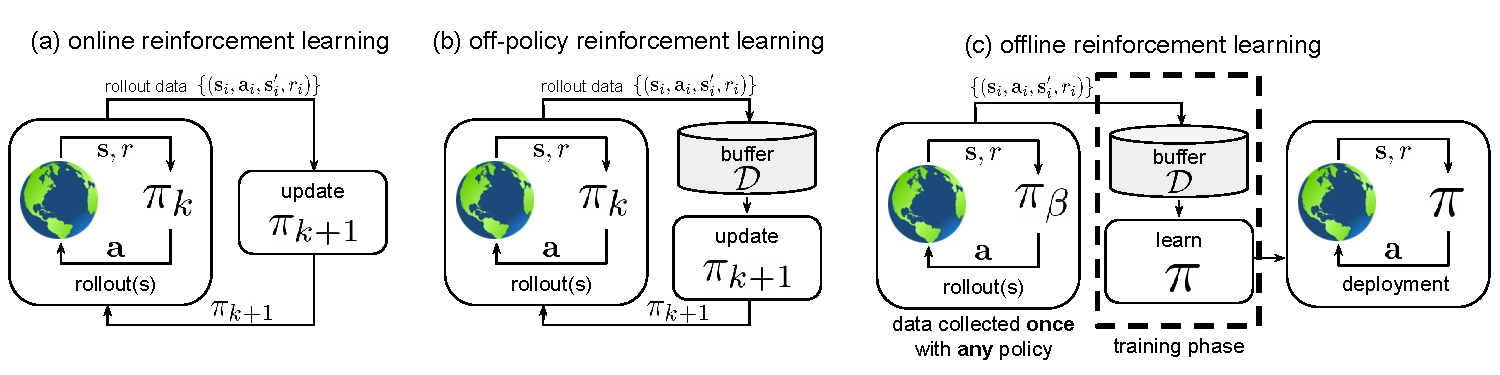
\includegraphics[height=1.5in]{figs/offlineRL}
\caption{
  Comparison of online on-policy RL,  online off-policy RL,
  and offline RL.
\figtaken{Figure 1 of \citep{Levine2020offline}}.
\figthanks{Sergey Levine}.
}
\label{fig:offline}
\end{figure}




\keywordDef{Offline reinforcement learning}
(also called \keywordDef{batch reinforcement learning} \cite{Lange2012})
is concerned with learning a reward maximizing
policy from a fixed, static dataset,
collected by some existing policy,
known as the \keywordDef{behavior policy}.
Thus no interaction with the environment is allowed
(see \cref{fig:offline}).
This makes policy learning harder than the online case,
since we do not know the consequences of actions that were not taken
in a given state, and cannot test any such ``counterfactual'' predictions
by trying them.
(This is the same problem as in off-policy RL, which we discussed in
\cref{sec:offpolicy}.)
In addition, the policy will be deployed on new states that it may not have seen,
requiring that the policy generalize out-of-distribution,
which is the main bottleneck for current offline RL methods \citep{Park2024value}.
%We discuss some solution methods below.
%(See also \citep{Bhargava2024} for a recent comparison
%of the methods we will discuss.)

A very simple and widely used offline RL method
is known as \keyword{behavior cloning} or \keyword{BC}.
This amounts to training a policy to predict the observed
output action $a_t$ associated with each observed state $s_t$,
so we aim to ensure $\pi(s_t) \approx a_t$,
as in supervised learning.
This assumes the offline dataset was created by an expert,
and so falls under the umbrella of imitation learning
(see \cref{sec:BC} for details).
By contrast, offline RL methods can leverage suboptimal data.
We give a brief summary of some of these  methods below.
For more details, 
see e.g., \citep{Levine20Offline,Chen2024offlineRL,Cetin2024}.
For some offline RL benchmarks,
see DR4L \citep{Fu20}, RL Unplugged \citep{Gulcehre20},
OGBench (Offline Goal-Conditioned benchmark) \citep{Park2024},
and D5RL \citep{Rafailov2024}.

%A simple extension of BC to the case where
%the offline dataset was generated by policies of variable
%quality is to filter out trajectories with low reward;
%this is called \keywordDef{filtered BC}.




%For an experimental comparison of
%offline RL methods, see e.g., \citep{Gulcehre20,Fu20,Bhargava2024,Cetin2024}.
%For a more recent approach,
%known as \keywordDef{perceiver actor critic},
%see \citep{Springenberg2024}.


\subsection{Offline model-free RL}


In principle, we can tackle offline RL using the off-policy methods
that we discussed in \cref{sec:offpolicy}.
These use some form of importance sampling, based on
$\policytgt(a|s)/\behavior(a|s)$, to reweight the data in the replay buffer $\data$,
which was collected by 
the behavior policy, towards the current policy (the one  being evaluated/ learned).
Unfortunately, such methods only work well if the behavior policy is
is close to the new policy. In the online RL case,
this can be ensured by gradually updating the new policy away from
the behavior policy, and then sampling new data  
from the updated policy (which becomes the new behavior policy).
Unfortunately, this is not an option in the offline case.
Thus we need to use other strategies to control the discrepancy
between the behavior policy and learned policy, as we discuss below.
(Besides the algorithmic techniques we discuss,
another reliable way to get better offline RL performance
is to train on larger, more diverse datasets,
as shown in \citep{Kumar2023offline}.)

\eat{
Various methods have been developed to control the variance
of the importance weights in the offline case,
as discussed in \citep[Sec 4]{Levine20Offline},
but such methods are not widely used in practice.
}

\subsubsection{Policy constraint methods}

In the \keywordDef{policy constraint} method,
we use a modified form of  actor-critic,  which, at iteration $k$,
uses an update of the form
\begin{align}
  Q^{\pi}_{k+1} &\leftarrow \argmin_Q \expectQ{
    \left(Q(s,a) - (R(s,a) + \gamma \expectQ{Q^{\pi}_k(s',a')}{\pi_k(a'|s')})
    \right)^2
  }{(s,a,s') \sim \data} \\
  \pi_{k+1} &\leftarrow \argmax_{\pi} \expectQ{
    \expectQ{Q^{\pi}_{k+1}(s,a)}{\pi(a|s)}}{s \sim \data}
  \myst D(\policy, \behavior) \leq \epsilon
  \label{eqn:piUpdate}
\end{align}
where $D(\policy(\cdot|s), \behavior(\cdot|s))$ is a divergence measure
on distributions, such as KL divergence or another $f$-divergence.
This ensures that we do not try to evaluate the $Q$ function
on actions $a'$ that are too dissimilar from those seen
in the data buffer (for each sampled state $s$),
which might otherwise result in artefacts similar
an  adversarial attack.


As an alternative to adding a constraint,
we can add a penalty of
$\alpha D(\policy(\cdot|s), \behavior(\cdot|s))$
to the target $Q$ value and the actor objective,
resulting in the following update:
\begin{align}
  Q^{\pi}_{k+1} &\leftarrow \argmin_Q \expectQ{
    \left(Q(s,a) - (R(s,a) + \gamma \expectQ{Q^{\pi}_k(s',a')
    -\alpha \gamma D(\pi_k(\cdot|s'), \behavior(\cdot|s'))}{\pi_k(a'|s')})
    \right)^2
  }{(s,a,s') \sim \data} \\
  \pi_{k+1} &\leftarrow \argmax_{\pi} \expectQ{
    \expectQ{Q^{\pi}_{k+1}(s,a)}{\pi(a|s)}
  - \alpha D(\pi(\cdot|s'), \behavior(\cdot|s'))}{s \sim \data}
\end{align}

One problem with the above method is that we have to fit
a parametric model to $\behavior(a|s)$ in order to evaluate the
divergence term. Fortunately, in the case of KL, the divergence
can be enforced implicitly,
as in the \keywordDef{advantage weighted regression}
or \keywordDef{AWR} method of \citep{Peng2019awr},
the \keywordDef{reward weighted regression} method
of \citep{Peters07},
 the \keywordDef{advantage weighted actor critic}
or \keywordDef{AWAC} method of \citep{Nair2020},
the \keywordDef{advantage weighted behavior model}
or \keywordDef{ABM} method of \citep{Siegel2020},
In this approach, we first solve (nonparametrically) for the new policy
under the KL divergence constraint to
get $\overline{\pi}_{k+1}$, and then we project
this into the required policy function class via
supervised regression, as follows:
\begin{align}
  \overline{\pi}_{k+1}(a|s) &\leftarrow \frac{1}{Z}
  \behavior(a|s) \exp\left( \frac{1}{\alpha} Q_k^{\pi}(s,a) \right) \\
  \pi_{k+1} &\leftarrow \argmin_{\pi} \KLpq{\overline{\pi}_{k+1}}{\pi}
\end{align}
In practice the first step can be implemented by weighting
samples from $\behavior(a|s)$ (i.e., from the data buffer)
using importance weights given by
$\exp\left( \frac{1}{\alpha} Q_k^{\pi}(s,a) \right)$,
and the second step can be implemented via  supervised
learning (i.e., maximum likelihood estimation) using
these weights.

It is also possible to replace the KL divergence
with an integral probability metric (IPM),
such as the maximum mean discrepancy (MMD) distance,
which can be computed from samples,
without needing to fit a distribution $\behavior(a|s)$.
This approach is used in 
\citep{Kumar2019off}.
% https://bair.berkeley.edu/blog/2019/12/05/bear/
This has the advantage that it can constrain the support of the learned
policy to be a subset of the behavior policy,
rather than just remaining close to it.
To see why this can be advantageous, consider the case where
the behavior policy is uniform.
In this case, constraining the learned policy to remain close (in KL divergence)
to this distribution could result in suboptimal behavior,
since the optimal policy may just want to put all its mass on a single action
(for each state).

\subsubsection{Behavior-constrained policy gradient methods}

Recently a class of methods has been developed that is simple and effective:
we first learn a baseline policy $\pi(a|s)$ (using BC) and a Q function
(using Bellman minimization) on the offline data,
and then update the policy parameters to pick actions that have high expected
value according to $Q$ and which are also likely under the BC prior.
%which we call behavior-regularized PG \citep{Wu2020}.
An early example of this is the $Q^{\dagger}$ algorithm
of \citep{Fujimoto2019batch}.
In  \citep{Fujimoto2021}, they present
 the \keywordDef{DDPG+BC} method,
which optimizes
\be
\max_{\pi} J(\pi) = \expectQ{
  Q(s,\mu^{\pi}(s)) + \alpha \log \pi(a|s)}{(s,a) \sim \data}
\ee
where $\mu^{\pi}(s) = \expectQ{a}{\pi(a|s)}$ is the mean of
the predicted action, and $\alpha$ is a hyper-parameter.
As another example,
the \keywordDef{DQL} method of \citep{Wang2023DQL}
optimizes a diffusion policy using
\be
\min_{\pi} \loss(\pi)
= \loss_{\text{diffusion}}(\pi) + \loss_{q}(\pi)
= \loss_{\text{diffusion}}(\pi) 
- \alpha \expectQ{Q(s,a)}{s \sim  \data,
  a \sim \pi(\cdot|s)}
\ee
Finally, \citep{Agarwal2022} discusses how to transfer
the policy from a previous agent to a new agent
by combining BC with Q learning.

\subsubsection{Uncertainty penalties}
\label{sec:offlineUncertainty}

An alternative way to avoid picking out-of-distribution actions,
where the $Q$ function might be unreliable,
is to add a penalty term to the $Q$ function based on the estimated
epistemic uncertainty, given the dataset $\data$,
which we denote by $\text{Unc}(P_D(Q^{\pi}))$,
where $P_D(Q^{\pi})$ is the distribution over $Q$ functions,
and $\text{Unc}$ is some metric on distributions.
For example, we can use a deep ensemble to represent the distribution,
and use the variance of $Q(s,a)$ across ensemble members as
a measure of uncertainty.
%as in \citep{Kumar2019off}.
This gives rise to the following policy improvement update:
\begin{align}
  \pi_{k+1} &\leftarrow \argmax_{\pi} \expectQ{
    \expectQ{
      \expectQ{Q^{\pi}_{k+1}(s,a)}{P_D(Q_{k+1}^{\pi})}
    }{\pi(a|s)}
    - \alpha \text{Unc}(P_D(Q_{k+1}^{\pi}))
}{s \sim \data}
\end{align}
For examples of this approach, see e.g.,
\citep{An2021,Wu2021unc,Ghasemipour2022}.

\subsubsection{Conservative Q-learning and pessimistic value functions}
\label{sec:CQL}
% Sergey Levine talk 2024
% https://www.youtube.com/watch?v=Az5BoT7lCYo&list=PLEA9Mnr-L18lI_I-EkyAc1-gXgBj52oV5


An alternative to explicitly estimating uncertainty
is to add a \keywordDef{conservative penalty}
directly to the $Q$-learning error term.
That is, we minimize the following wrt $\vw$
using each batch of data $\calB$:
\be
\overline{\calE}(\calB,\vw)
   = \alpha \calC(\calB,\vw) + \calE(\calB, \vw)
\ee
where $\calE(\calB, \vw) = \expectQ{ (Q_{\vw}(s,a) -
  (r+\gamma \max_{a'} Q_{\vw}(s',a')))^2}{(s,a,s') \in \calB}$
is the usual loss for $Q$-learning,
and $\calC(\calB,\vw)$ is some conservative penalty.
In the \keywordDef{conservative Q learning}
or \keywordDef{CQL} method of \citep{CQL},
we use the following penalty term:
\be
\calC(\calB,\vw)
= \expectQ{Q_{\vw}(s,a)}{s \sim \calB, a \sim \pi(\cdot|s)}
- \expectQ{Q_{\vw}(s,a)}{(s,a) \sim \calB}
\ee
If $\pi$ is the behavior policy, this penalty becomes 0.

 
\eat{
A natural approach to offline RL is to just perform
Q-learning on the fixed dataset,
and then to compute the policy using
$\pi(a|s) = \argmax_a Q(s,a)$.
In principle this should work, since Q-learning is off-policy,
but in practice it does not work.
The reason is that Q-learning is trying to learn
the optimal policy $\pi^*$, but the data was generated by
a fixed \keyword{behavior policy}
$\pi_{\beta}$, so when Q-learning predicts the value
of the best action, it cannot be checked against the data,
and it might become over optimistic.



To see this in more detail, let us rewrite
the Bellman backup in terms of a distribution
$\pi_{\tnew}$ that puts all its mass on the optimal action
(according to the current $Q$) for each state,
so $\pi_{\topt}(a|s)=\delta(a-\argmax_{a'} Q(s,a'))$.
Thus the TD loss becomes
\be
J_{\beta}(Q,\pi) = \expectQ{ (Q(s,a)-\targetV(s,a))^2}{\pi_{\beta}(s,a)}
\ee
where the target $\targetV(s,a)$ is defined by 
\be
\targetV(s,a) =
  r(s,a) + \expectQ{Q(s',a')}
  {\pi_{\beta}(s') \pi_{\topt}(a'|s')}
\ee
If we have $\pi_{\beta}(s,a)=\pi_{\beta}(s) \pi_{\topt}(s|a)$, this optimization
should work well, since the training data comes
from the optimal distribution, and thus we have a stable system.
But for suboptimal behavior data, Q-learning will learn
to find actions that do better than the training data,
according to $Q$; this is like finding adversarial examples
for a network, and can result in unstable behavior,
where the estimated $Q$ values increase, but the actual reward
decreases.

% Pessimism-based methods eg CQL
% Policy constraints (eg BRAC)
% Avoid OOD actions in updates (eg AWAC, IQL). Don't evaluate
%  actions you didn't train on.

One way to deal with the overestimation problem is to use
 \keywordDef{conservative Q learning}
 or \keywordDef{CQL} \citep{CQL}.
The idea is to find $(s,a)$ points where the
$Q$-function might be overestimating the true value,
and then to ``push down'' on the estimate,
so it becomes more conservative.
In practice this amounts to adding the following
regularizer (scaled by $\alpha$) to $J_{\beta}$:
\begin{align}
J_{CQL}(Q,\pi)
&=   \expectQ{ Q(s,a) -\expectQ{Q(s,a')}{a' \sim \pi(\cdot|s)}
}{(s,a) \sim \data} \\
&=  \expectQ{Q(s,a)}{(s,a) \sim \data}
- \expectQ{Q(s',a')}{s' \sim \data, a' \sim \pi(\cdot|s')}
\label{eqn:CQL}
\end{align}
%The first term in the regularizer pushes down on all
%$Q$ values, whereas the second term pushes up on
%the $Q$ values encountered in the data.
%One can prove that
%$\hat{Q}^{\pi} \leq Q^{\pi}$ for large enough $\alpha$.
%The $\alpha$ coefficient determines the strength of this
%regularization.


}

 \eat{
the approach attempts to generalize beyond  offline data,
but not too far.
First it uses Q learning to solve
\be
\argmin_{\vw} [Q_{\vw}(s_t,a_t) - \expectQ{r(s_t,a_t) + Q_{\vw}(s_{t+1},a_{t+1})}{\pemp}]^2
\ee
where $\pemp$ is the empirical distribution over trajectories.
It also fits the BC policy $q_{\beta}(a_t|s_t)$.
Finally  it finds the policy that is closest
(in the chosen parametric family)
to
$q(a_t|s_t) \propto \exp(Q_{\vw}(s_t,a_t) q_{\beta}(a_t|s_t))$,
which is the BC policy weigthed  by the Q function.
It does this by solving a weighted MLE problem
\be
\argmin_{\vtheta} \KLpq{\pi_{\vtheta}(a_t|s_t)}{q(a_t|s_t)}
\ee
%
 }


     
\subsection{Offline model-based RL}
\label{sec:offlineMBRL}


In \cref{sec:MBRL}, we discussed model-based RL,
which can train a dynamics model given a fixed dataset,
and then use this to generate synthetic data
to evaluate and then optimize  different possible policies.
However, if the model is wrong, the method may learn a suboptimal
policy, as we discussed in \cref{sec:modelUncertainty}.
This problem is particularly severe in the offline RL case,
since we cannot recover from any errors by collecting more data.
Therefore various conservative MBRL algorithms have been developed,
to avoid exploiting model errors.
For example, \citep{Kidambi2020} present the
\keywordDef{MOREL} algorithm,
and \citep{Yu2020mopo} present the \keywordDef{MOPO} algorithm.
Unlike the
value function uncertainty method of \cref{sec:offlineUncertainty},
or the conservative value function method of \cref{sec:CQL},
these model-based methods add a penalty for visiting states where
the model is likely to be incorrect.

In more detail, let $u(s,a)$ be an estimate of the uncertainty of the
model's predictions given input $(s,a)$.
In MOPO, they define a conservative reward using
$\overline{R}(s,a) = R(s,a) - \lambda u(s,a)$,
and in MOREL, they modify the MDP so that the agent enters an
absorbing state with a low reward when $u(s,a)$ is sufficiently
large.
In both cases, it is possible to prove that the model-based
estimate of the policy's performance under the modified
reward or dynamics is a lower bound of the performance
of the policy's true performance in the real MDP,
provided that the uncertainty function $u$ is an error oracle,
which means that is satisfies
$D(M_{\vtheta}(s'|s,a), M^*(s'|s,a)) \leq u(s,a)$,
where $M^*$ is the true dynamics, and $M_{\vtheta}$
is the estimated dynamics.

For more information on offline MBRL methods,
see \citep{Chen2024offline}.



 
\subsection{Offline RL using reward-conditioned sequence modeling}
\label{sec:seqModel}

Recently an approach to offline RL
based on sequence modeling has become very popular.
The basic idea --- known as \keywordDef{upside down RL}
\citep{Schmidhuber2019}
or \keywordDef{RvS} (RL via Supervised learning)
\citep{Kumar2019,Emmons2021} ---
is to train a generative model over future states
and/or actions conditioned on the observed reward,
rather than predicting the reward given a state-action
trajectory.
%This reduces to a supervised learning problem
%(albeit with high dimensional output).
At test time, the conditioning is changed
to represent the desired reward, and futures
are sampled from the model.
The implementation of this idea then depends on what
kind of generative model to use, as we discuss below.

The \keywordDef{trajectory transformer}
method of \citep{trajectoryTransformer}
learns a joint model of the form
$p(\vs_{1:T}, \va_{1:T}, \vr_{1:T})$
using a transformer,
and then samples from this using beam search,
selecting the ones with high reward (similar to MPC, \cref{sec:MPC}).
The \keywordDef{decision transformer} \citep{decisionTransformer}
is related, but  just generates action sequences,
and conditions on the past observations and the future reward-to-go.
That is, it fits
\be
\argmax_{\vtheta} \expectQ{
  \log \pi_{\vtheta}(a_t|s_{0:t}, a_{0:t-1}, \text{RTG}_{0:t})}{\pemp}
\ee
where $\text{RTG}_t = \sum_{k=t}^T r_t$ is the return to go.
(For a comparison of decision transformers to other offline RL methods,
see \citep{Bhargava2024}.)

The \keywordDef{diffuser} method of \citep{diffuser}
is a diffusion version of trajectory transformer,
so it fits $p(\vs_{1:T}, \va_{1:T}, \vr_{1:T})$ using diffusion,
where the action space is assumed to be continuous.
They also replace beam search with classifier guidance.
The \keywordDef{decision diffuser} method of \citep{decisionDiffuser}
extends diffuser by using classifer-free guidance,
where the conditioning signal is the reward-to-go,
simlar to decision transformer.
However, unlike diffuser,
the decision diffuser just models the future state trajectories
(rather than learning a joint distribution over states and actions),
and infers the actions using an \keywordDef{inverse dynamics model}
$a_t = \pi(s_t, s_{t+1})$,
which is trained using supervised learning.

One problem with the above approaches is that conditioning
on a desired return and taking the predicted action can fail dramatically
in stochastic environments,
since trajectories that result in a return may have only
achieved that return due to chance \citep{Paster2022,Yang2023,Brandfonbrener2022,Villaflor2022}.
(This is related to the optimism bias in the control-as-inference
approach discussed in \cref{sec:RLAI}.)

 
\subsection{Hybrid offline/online methods}

Despite the progress in offline RL, it is fundamentally
more limited in what it can learn compared to online RL
\citep{Ostrovski2021}.
Therefore, various hybrids of offline and online RL have been proposed,
such as
\citep{Ball2023} and \citep{Nakamoto2023}.

For example,
\citep{Nakamoto2023}
suggest pre-training
with offline RL (specifically CQL) followed by online finetuning.
Naively this does not work that well, because CQL can be
too conservative, requiring the online learning
to waste some time at the beginning fixing
the pessimism. So they propose a small
modification to CQL,
known as \keywordDef{calibrated Q learning}.
This simply prevents CQL from being too conservative,
by replacing the CQL
regularizer
%in \cref{eqn:CQL}
with
\be
\min_Q \max_{\pi}
J(Q,\pi)    + \alpha  \expectQ{
  \max(Q(s,a), V^{\pi_{\beta}}(s))
  - \alpha \expectQ{Q(s,a)}{(s,a) \sim \data}
}{s \sim \data, a \sim \pi(a|s)}
\label{eqn:CalQL}
\ee
where the $Q(s,a)$ term inside the $\max$
ensures conservatism (so $Q$ lower bounds
the value of the learned policy),
and the $V^{\pi_{\beta}}(s)$ term
ensures ``calibration''
(so $Q$ upper bounds the value
of the behavior policy).
Then online finetuning is performed in the usual way.

%This seems like a promising practical solution
%for creating RL systems that work in the real-world.





\section{Extreme-token Phenomena in pretrained LLMs} \label{sec:llm}

%\DP{TODO for SONG: rewrite this paragraph}
% \DP{TODO for DRUV: check again after Song finishes}

In this section, we investigate extreme-token phenomena in open-source pretrained LLMs. In \Cref{sub:active_dormant}, we analyze the static behavior of these phenomena in Llama 2-7B-Base \citep{touvron2023llama}, confirming the existence of the \textit{active-dormant mechanism} in LLMs. Notably, we identify a specific head that is active on GitHub samples but dormant on Wikipedia samples. In \Cref{sub:olmo_dynamics}, we examine the dynamic behavior of extreme-token phenomena during the pretraining of OLMo-7B \citep{groeneveld2024olmo}. We show that the attention logits, value states norm, and residual states norm of the sink token(s) in OLMo reflect behavior similar to that of the simpler BB model. Specifically, the simultaneous formation of attention sinks and value-state drains gives evidence for the \textit{mutual reinforcement mechanism}.

% It turns out that our exploration into the BB task in \Cref{sec:bb_task} may actually shed light upon the origin of attention sinks, small value states, and massive norms in full-fledged large language models trained on massive amounts of text. To verify this claim, we once again summarize and elaborate the observations we made in the BB task model:
% \begin{enumerate}[leftmargin=2em]
% \setlength\itemsep{0pt}
%     \item The attention sinks and value-state drains are external manifestations of the active-dormant mechanism in LLMs. 
%     \item The lower-layer components (e.g., attentions and MLPs) of the LLM contribute to all three extreme-token phenomena.     
%     \item The attention heads go through the attention-increasing and value-state-shrinking phase. They converge to the stable phase, with identical attention logits on the \bos~token. Meanwhile, the residual state norm corresponding to the \bos{} token linearly increase during pretraining.
% \end{enumerate}

% We will confirm each of these observations in this section.\footnote{Here, we mention that in order to achieve this checklist, we had to do a certain amount of translating from the setting of the BB model to the setting of LLMs. For example, the BB model identifies trigger tokens as the (semantically) important tokens in that the model should change behavior after seeing them. In the context of LLMs, almost every token fits this description for a suitable context, but tokens like \bos{} do not. 
% %\tianyu{I think we should say that each token could be trigger or non-trigger, depending on the context? If every tokens are triggers, there's no dormant phase.}
% } Namely, in \Cref{sub:active_dormant} we will confirm point 1; in \Cref{sub:circuits} we confirm point 2; and in \Cref{sub:olmo_dynamics} we confirm point 3.


\subsection{Active-dormant mechanism in LLMs}\label{sub:active_dormant}


\begin{figure}
    \centering
    \begin{subfigure}[t]{0.58\textwidth}
        \centering
        \caption{\small Attention weights for GitHub/Wikipedia data}% \sm{Maybe 2 by 2? }}
        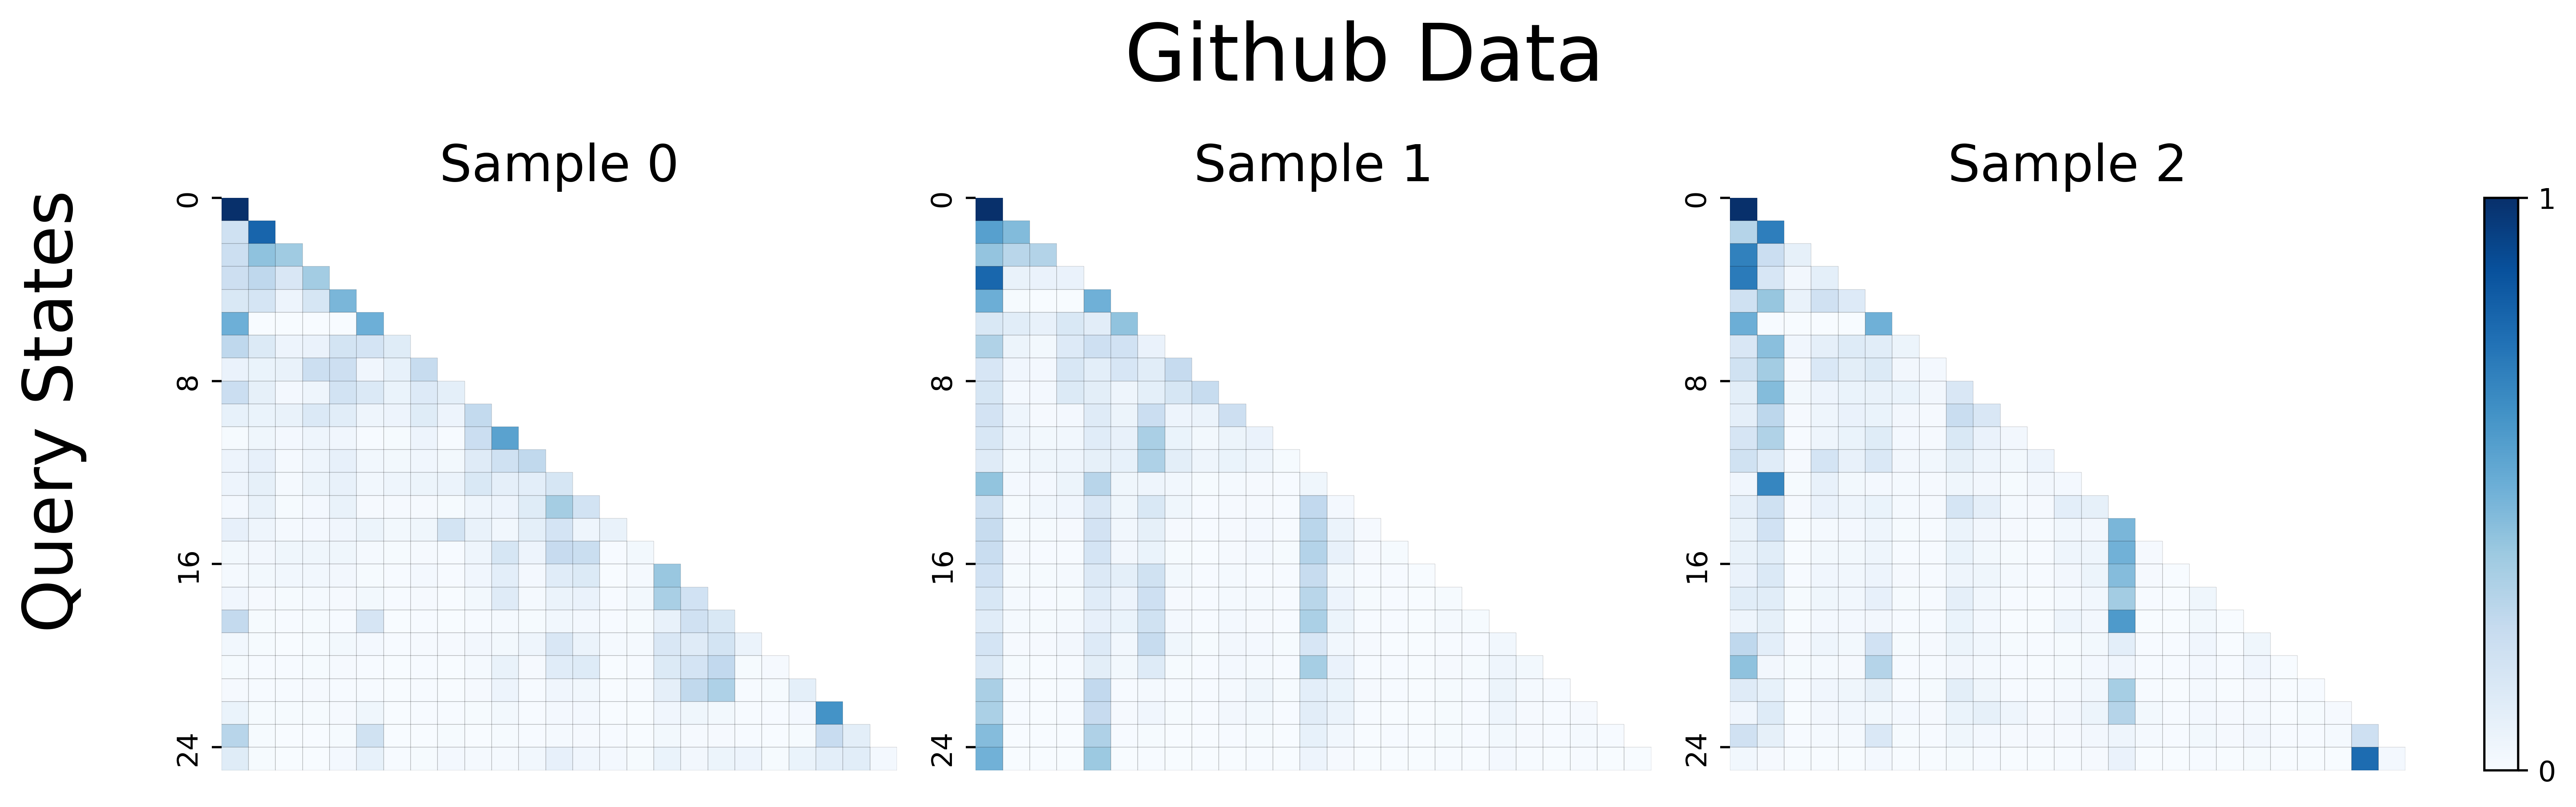
\includegraphics[width=0.9\textwidth]{Figures/L16_H25/attn_github_head25.png}
        
        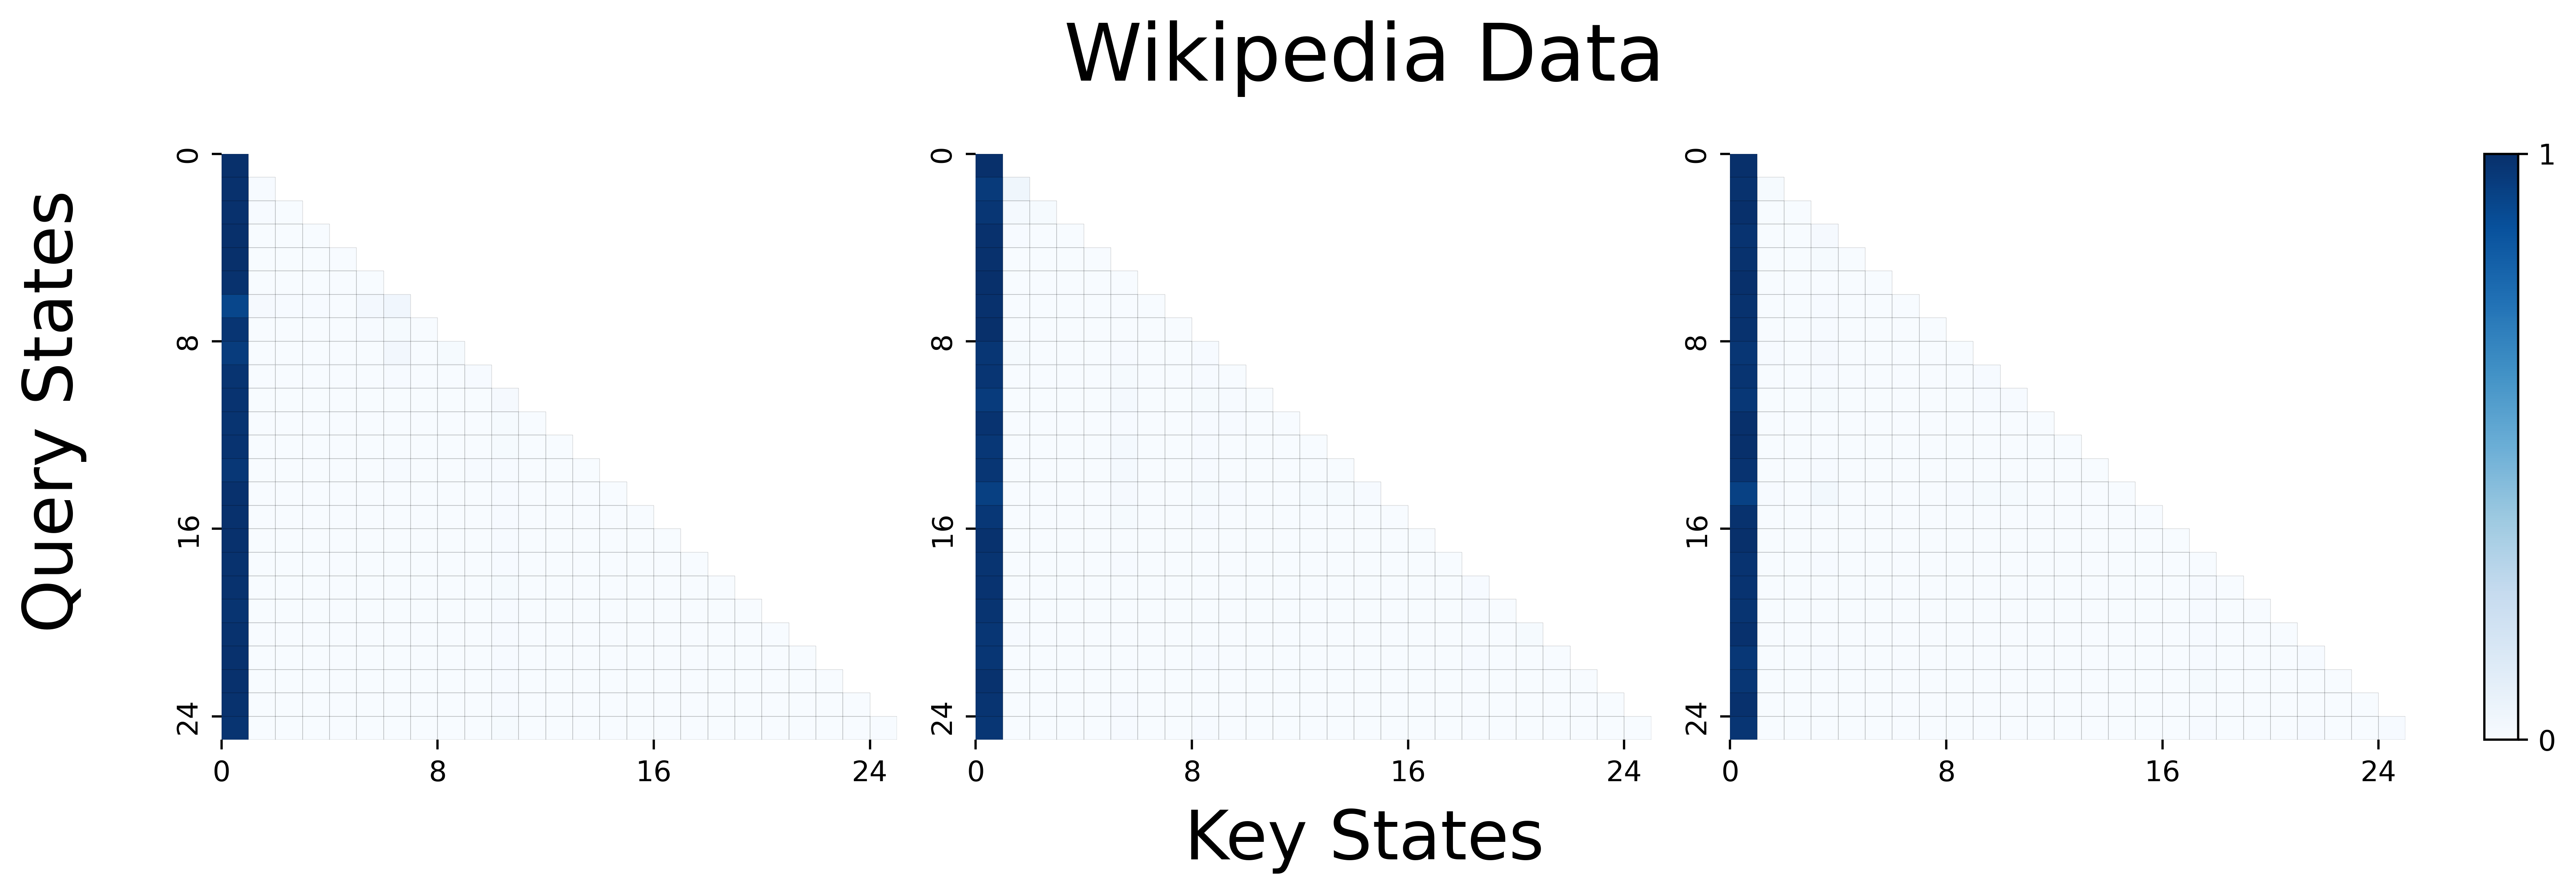
\includegraphics[width=0.9\textwidth]{Figures/L16_H25/attn_wikipedia_head25.png}
        \label{fig:github_wikipedia_weights}
    \end{subfigure}
    \hfill
    \begin{subfigure}[t]{0.38\textwidth}
        \caption{\small Zero-out-head intervention outcomes}
        \label{fig:github_wikipedia_zero_out}
        \vskip1.5em
        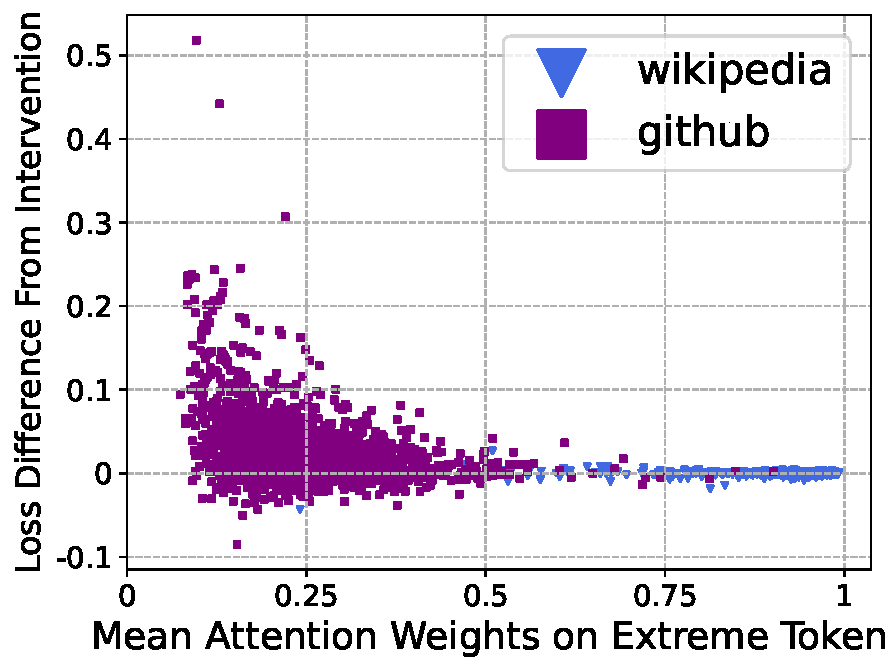
\includegraphics[width=0.9\textwidth]{Figures/BBM/LLM_interventions.pdf}
    \end{subfigure}
    \vspace{-0.5em}
    %\includegraphics[width=0.5\linewidth]{}
    \caption{\small \textbf{Active-dormant mechanism of Layer 16 Head 25 (L16H25) of Llama 2-7B-Base.} We observe that L16H25 is active on GitHub data and dormant on Wikipedia data, both sourced from RedPajama-1T \citep{together2023redpajama}. \textit{Left (a)}: Attention weights of L16H25, prompted by three randomly selected samples from each domain. \textit{Right (b)}: Results of an intervention study showing the change in cross-entropy loss when the output of L16H25 (specifically, its value states) is set to zero across sequences in both domains. The findings indicate that the model's performance for GitHub data, measured by cross-entropy loss, strongly relies on the output of this attention head. 
    % \sm{(a) Truncate at $24$ \sm{right: xlabel and xtick size. $x 0.1$} \sm{High priority} \sm{Orange color change}}
    % heads are sinks in one domain and not others (Llama 2 7B L16H25, GitHub vs Wikipedia) \DP{TODO...}
    % \DP{Plan: two figures. Left: attn sink visualization for GitHub on left and Wikipedia (4x4 (adjust to be visually appealing) samples visualize L16H25). Right: causal intervention, zeroing out head vs cross entropy delta taken across many samples from GitHub and Wikipedia.}
    }
    \label{fig:dormant_heads_domain_dependent}
\end{figure}




    %\textit{If all tokens at a head do not have helpful value states for predicting the next token, then attention mass will concentrate on tokens which are generally unhelpful for next-token prediction (like \bos). \sm{Attention heads are controlled by the active-dormant mechanism; attention sinks and value-state drains are the dormant phases of attention heads. }}

Our study of the BB model leads to the following prediction with respect to the extreme-token phenomena, which we hypothesize also applies to LLMs:  
\begin{center}
    \textit{Attention heads are controlled by an active-dormant mechanism (cf.\ Claim \ref{claim:active-dormant}). The presence of attention sinks and value-state drains indicates that an attention head is in a dormant phase.}
\end{center}

This hypothesis suggests that in LLMs, whether an attention head becomes a sink depends on the context. Specifically, the attention head may become entirely irrelevant for selecting the next tokens in certain contexts or tasks, but not in others. When this irrelevance occurs, the attention head transitions into an attention sink. This hypothesis was confirmed in small transformers and the BB task, as demonstrated in Section~\ref{sec:bb_task}. 



Accordingly, we aim to identify instances of attention heads in pretrained LLMs that exhibit this active-dormant behavior, i.e., heads that are dormant in some domains but active in others. In \Cref{fig:dormant_heads_domain_dependent}, we display a particular attention head---Layer 16 Head 25 (L16H25) of Llama 2-7B-Base \citep{touvron2023llama}---which demonstrates a clear active-dormant distinction across two distinct contexts (e.g., tokens from the GitHub subset versus the Wikipedia subset of RedPajama \citep{together2023redpajama}). While many attention heads show similar context-dependent behavior (see \Cref{sec:more_heads}), we focus on this one because the conditions for its activation are straightforward and interpretable, whereas other heads may have more nuanced criteria. 
% \sm{Can we plot more figures instead of the figures that are GitHub/Wiki}

\Cref{fig:github_wikipedia_weights} shows the attention maps of L16H25 on samples from both the GitHub and Wikipedia subsets of RedPajama. It demonstrates that L16H26 is \textit{dormant} (i.e., an attention sink) on samples from Wikipedia, which resemble prose, and \textit{active} (i.e., not an attention sink) on samples from GitHub, which resemble code. Additionally, \Cref{fig:github_wikipedia_zero_out} compares the loss difference when L16H25 is zeroed out for prompts from both domains. The results show that zeroing out this head significantly decreases model performance on GitHub sequences, while having minimal impact on Wikipedia sequences. This observation also confirms the head behaves as dormant in some contexts and active in others---in some contexts, removing this head has no effect on model performance, while in others, its removal causes significant performance drops.
% We include more detail in \Cref{sec:circuit}.
% , where we extract a circuit for extreme-token phenomena to examine the dormant-active mechanism and its interaction with input token semantics. \sm{Polish} \sm{Mid priority}



% Accordingly, we strive to find instances of heads in pretrained LLMs that satisfy this principle, i.e., which are dormant on some domains and active on others. In \Cref{fig:dormant_heads_domain_dependent}, we show a particular attention head -- Layer 16 Head 25 of Llama 2-7B-Base \citep{touvron2023llama} --- which has an extremely clear active-dormant distinction across two distinct contexts (e.g., tokens from RedPajama \citep{together2023redpajama} drawn from the GitHub subset versus the Wikipedia subset). While there are many such attention heads which are context-dependent --- we provide some in \Cref{sec:more_heads} --- we demonstrate this one because the conditions under which it is active are simple and interpretable, while others have more involved or complex criteria to become active. We observe that this attention head is \textit{dormant} (i.e., an attention sink) on samples from Wikipedia, which more closely resemble prose, and \textit{active} (i.e., not an attention sink) on samples from GitHub, which more closely resemble code. We also observe that this attention head, in general, contributes significantly to the performance of the model on code sequences, but has negligible impact on the performance of the model on prose sequences (\Cref{fig:github_wikipedia_zero_out}). This is a further justification, from a practical perspective, of why this head is sometimes dormant and sometimes active --- in some contexts we can ablate it from the model entirely with no effect, but in other contexts ablating the head leads to huge performance drops. We include more detail in \Cref{sec:circuit}, where we extract a circuit for extreme-token phenomena in order to analyze the dormant-active mechanism and its interaction with the semantics of the input tokens.

%\footnote{Llama 2-7B-Base has two sink tokens (\bos~and one more) in its attention sink heads, while Llama 3.1-8B-Base only has one (\bos). We discuss a potential reason in \Cref{sub:multiple_sinks_discussion}. \sm{Why we put this remark here?}} \sm{Talk about other heads also has dormant and active phase, though not interpretable. Ablation figures in appendix. } \DP{@SM: the first part is already in the paragraph.} \sm{It would be good to link to figures for other heads. } \DP{sure will add to appendix, and comment out this comments when done}

\subsection{Extreme-token phenomena along training dynamics of LLMs}\label{sub:olmo_dynamics}


\begin{figure}[t]
    \centering
    \begin{subfigure}[t]{0.32\textwidth}
        \centering 
        \caption{\small Attention sink dynamics}
        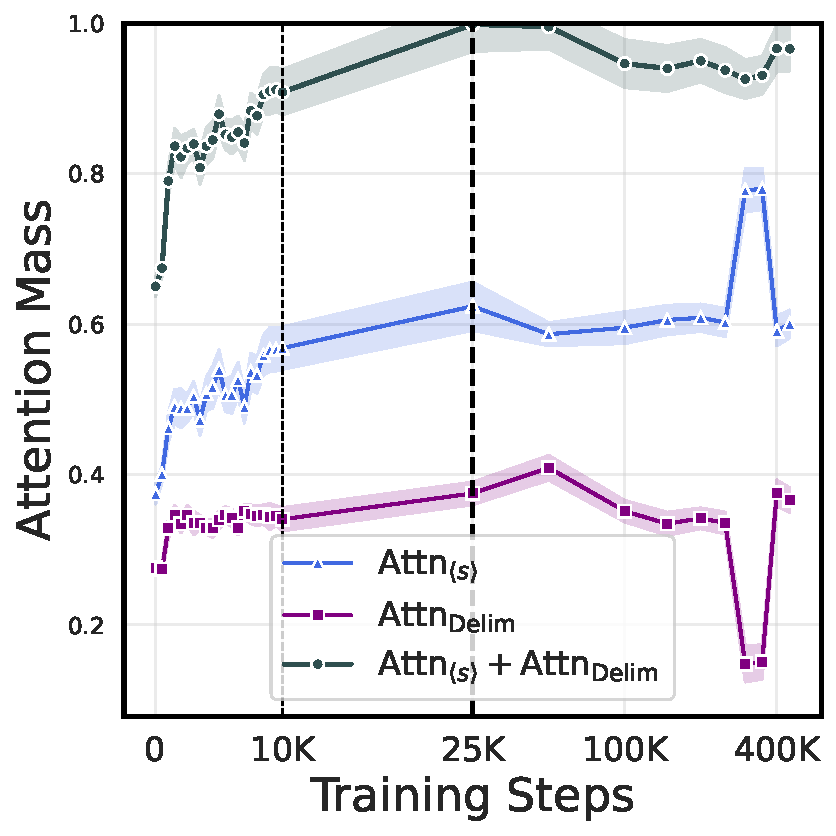
\includegraphics[width=0.9\textwidth]{Figures/olmo/attn_mass_on_top_two_tokens.pdf}
        \label{fig:olmo_sink}
    \end{subfigure}
    \begin{subfigure}[t]{0.32\textwidth}
        \centering 
        \caption{\small Value state dynamics}
        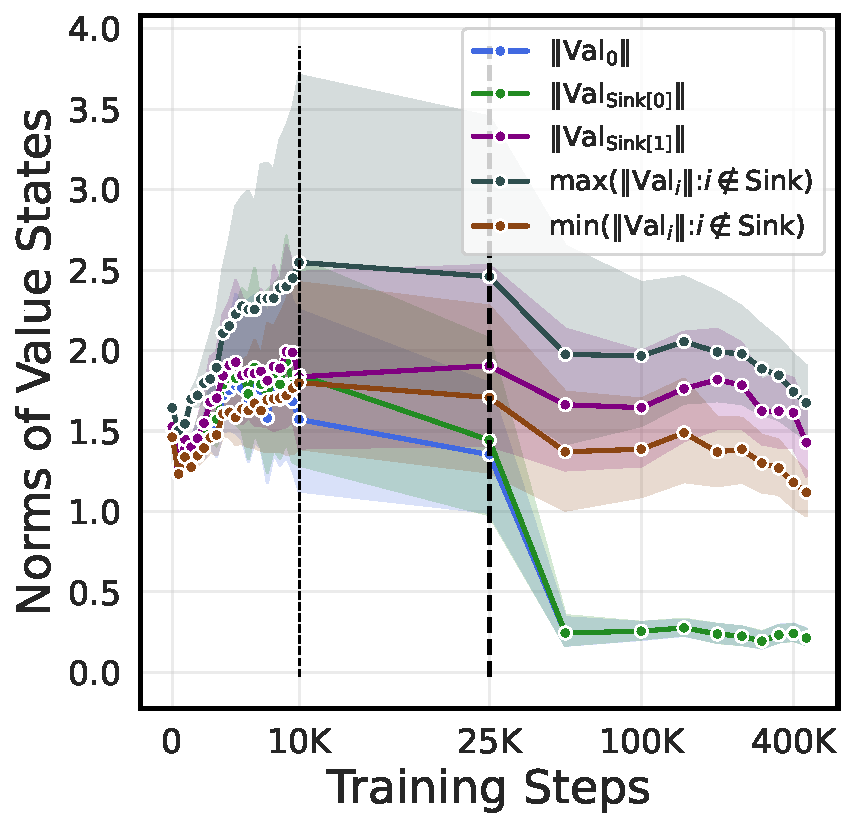
\includegraphics[width=0.9\textwidth]{Figures/olmo/value_norms.pdf}
        \label{fig:olmo_drain}
    \end{subfigure}
    \begin{subfigure}[t]{0.32\textwidth}
        \centering 
        \caption{\small Residual state dynamics}
        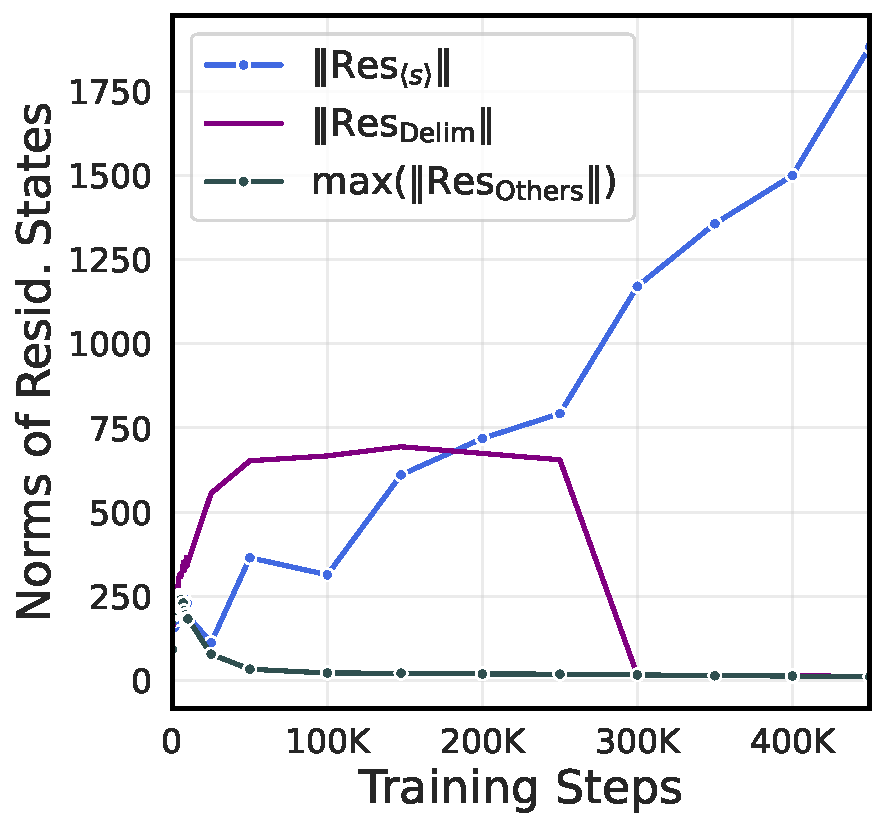
\includegraphics[width=0.9\textwidth]{Figures/olmo/layer_output_norms.pdf}
        \label{fig:olmo_peak}
    \end{subfigure}
    % \vspace{-2em}
    \caption{\small \textbf{Attention weights, value state norms, and residual state norms of Layer 24 during the training dynamics of OLMo.} \textit{Left (a)}: The total attention mass on extreme tokens \bos~and ``\text{Delim}''(\period) at Layer 24, averaged across all attention heads. The horizontal axis is logarithmically scaled after step $10$k. We observe a rapid increase followed by stabilization within the range \([0.9, 1]\) for the rest of training, consistent with our predictions. \textit{Middle (b)}: The value state norms of each token at Layer 24 during training, averaged over all heads. The horizontal axis is logarithmically scaled after step $10k$. Initially, the value states of all tokens shrink, eventually converging, while the value states of the extreme tokens shrink to significantly lower levels compared to other tokens. Figure \textit{(a)} and \textit{(b)} coincide with the trends in Figure~\ref{fig:dynamics} under the BB task. \textit{Right (c)}: The residual state norms of each token at Layer 24 during training. The residual state norm of \bos~increases linearly in magnitude throughout training, matching Figure~\ref{fig:sgd} in the BB task.}
    % \sm{Thicker} \sm{L24 is a bit repetitive} \sm{For (a) and (b), is there a way to draw 0 - 50K using linear scale and 50K - 500K using log scale? This could match better Figure 3(b)} \tianyu{link back to corresponding figures in BB task}}



    
    \label{fig:olmo_predictions_phase0}
\end{figure}
\begin{figure}[h]
    \centering
    \hfill
    \begin{subfigure}[t]{0.32\textwidth}
        \centering 
        \caption{\small Logit dynamics}
        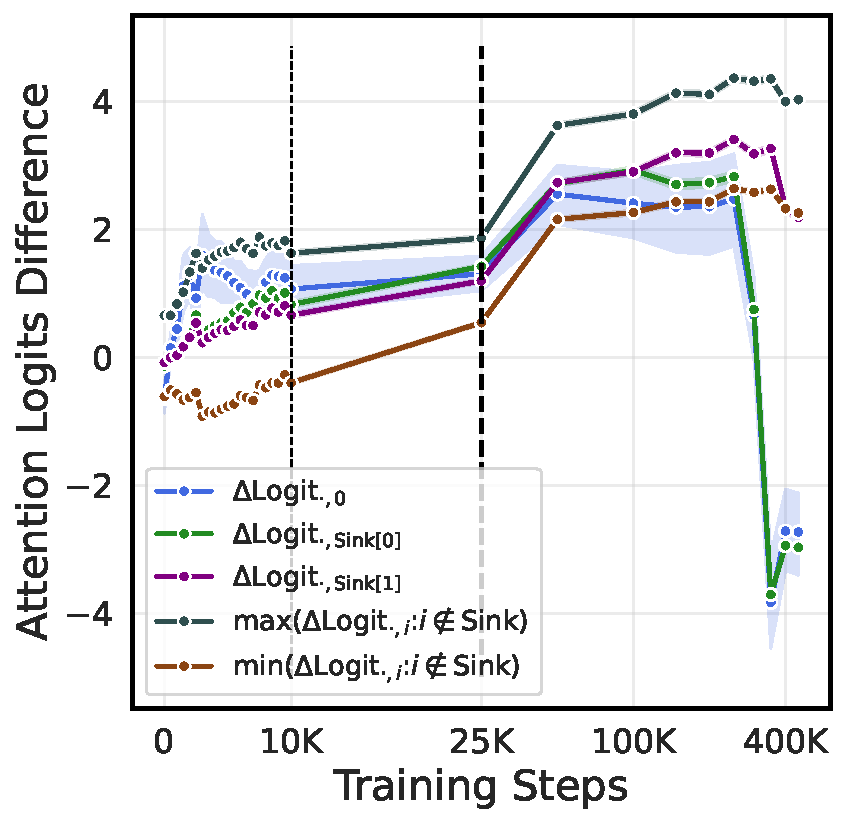
\includegraphics[width=0.9\textwidth]{Figures/olmo/attention_logits.pdf}
        \label{fig:attention_logits_olmo_dynamic}
    \end{subfigure}
    \hfill
    \begin{subfigure}[t]{0.32\textwidth}
        \centering 
        \caption{\small Sink-logits concentration}
        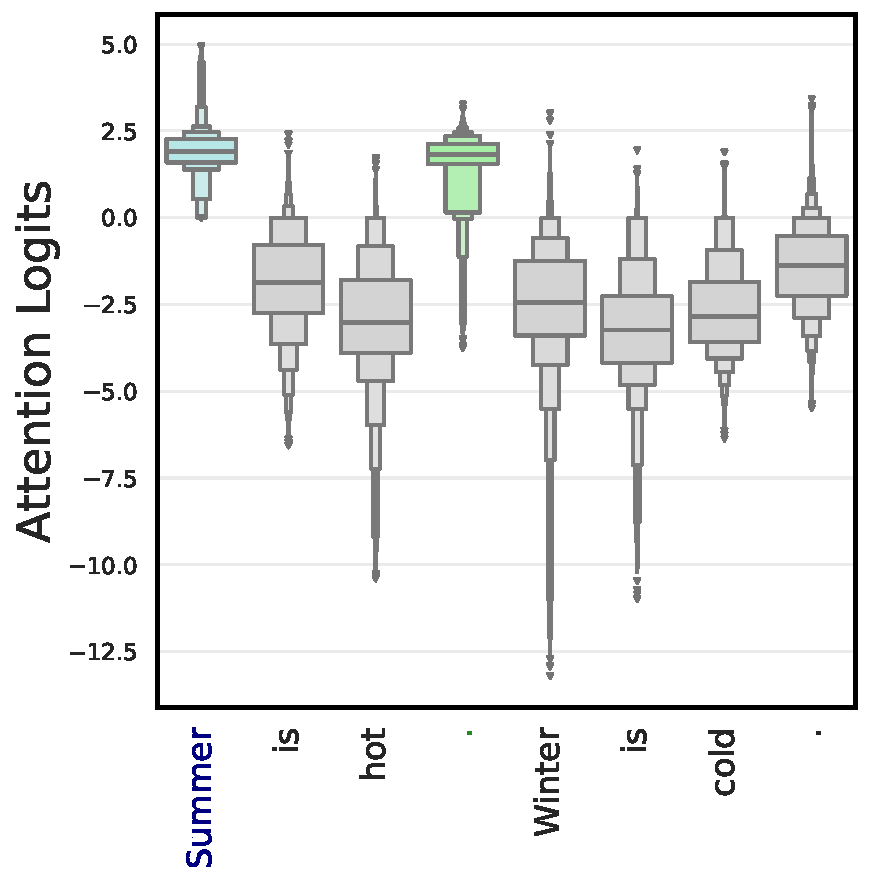
\includegraphics[width=0.9\textwidth]{Figures/olmo/attention_logits_on_test.pdf}
        \label{fig:attention_logits_olmo_static}
    \end{subfigure}
    \hfill
    \phantom{.}
    % \vspace{-2em}
        \caption{\small \textbf{Attention logits of Layer 24.}  \textit{Left (a)}: Attention logits difference of all tokens' query states against \bos's key state during training. The difference in attention logits is computed as \(\Delta\mathrm{logit}_{\cdot,\bos} = \query_{\cdot}^\top \key_{\bos} - \text{Mean}[\query_{\cdot}^\top \key_{\text{Others}}]\). The horizontal axis is logarithmically scaled after step $10k$. We observe that $\Delta \mathrm{logit}_{\cdot,\bos}$ increases approximately in logarithmic scale during training steps $10$k to $100$k, matching the decreasing phase of the value states in Figure~\ref{fig:olmo_drain}. 
        % This behavior aligns with the stable-phase prediction made in the BB model in \Cref{thm:main}(c). Note that this prediction does not apply to the logit corresponding to the zeroth query and key token, as its softmax value will be set to \(1\), making its behavior irrelevant for prediction. 
        \textit{Right (b)}: Attention logits of the last token's query state against all token's key states for pretrained OLMo. In this experiment, we generate \(128\) randomly sampled test tokens with IDs from \(100\) to \(50000\) in the OLMo tokenizer. We append each token separately to the test phrase ``Summer is warm\period~Winter is cold\period'', creating \(128\) different samples, which we feed to the LLM to examine the model behavior. We plot the distribution of (un-shifted) attention logits \( \text{logit}_{\cdot,\tok}=\query_{\mathrm{test}}^\top \key_{\tok}\) across all heads at Layer 24 and all test tokens. The distribution of $\text{logit}_{\cdot,\bos}$ and $\text{logit}_{\cdot,\text{Delim}}$ have considerably small variance compared with other logits, confirming the sink-logits concentration phenomenon. }
        % \tianyu{maybe to make it more clear, we can say that the variance of the attention logits on \bos~is small. Or we can use a new name (attention logits concentration)} \sm{tick size. Box thicker. } \sm{pdf} \tianyu{change the logit in (a)}}
    % \caption{\small \textbf{Attention logits of Layer 24.}  \textit{Left (a)}: The normalized attention logits of all tokens' query states against \bos's key state during training \sm{Is it the opposite?}. We observe that the logits of all non-extreme tokens' query states against \bos's key state in OLMo's Layer 24 are stable for a large fraction of the training run, after an initialization period. This echoes the stable phase prediction made in the BB model in \Cref{thm:main}(c). Note that this prediction makes no guarantees about the logit corresponding to the zeroth query token and zeroth key token, which will be set to \(1\) by the softmax and so its behavior is irrelevant for prediction. Also note that we use normalization, similar to \Cref{sec:bb_task}, to make all terms comparable; namely we have \(\mathrm{logit}_{i} = \langle \query_{i}, \key_{0}\rangle - \mathtt{mean}_{j}(\langle \query_{i}, \key_{j}\rangle)\). \textit{Right (b)}: \sm{A summary phrase of the figure.} For this experiment, we generate \(128\) randomly sampled test tokens with IDs from \(100\) to \(50000\) in the OLMo tokenizer. We append each token separately to the test phrase ``Summer is warm. Winter is cold.'', creating \(128\) different samples, which we feed to the LLM to record the model behavior. We plot the distribution of (un-normalized) dot products \(\langle \query_{\mathrm{test}}, \key_{j}\rangle\) across all heads at Layer 24 and all test tokens. We observe that logits of all regular tokens have very similar distributions, and the distributions of the logits corresponding to extreme tokens \(0\) and \(3\) are also similar. \sm{Why similar? } This confirms the hypothesis that at the end of training, attention heads converge to the stable phase, with similar logits on extreme tokens. \tianyu{maybe to make it more clear, we can say that the variance of the attention logits on \bos~is small. Or we can use a new name (attention logits concentration)} \sm{tick size. Box thicker. } }
    \label{fig:olmo_predictions_phase1}
\end{figure}


Our study of the BB model leads to the following prediction about the dynamical behavior of the extreme-token phenomena, which we hypothesize also applies to LLMs:  
\begin{center}
    \textit{Attention heads undergo an attention-increasing and value-state-shrinking phase driven by the mutual reinforcement mechanism (cf.\ Claim~\ref{claim:mutual-reinforcement}). This is followed by a stable phase, where all non-trigger tokens have large, nearly identical attention logits on the extreme token. Simultaneously, the residual state norms of the extreme tokens increase linearly during pretraining.}
\end{center}



% We confirm these predictions below, thus demonstrating the overall validity of the BB task as a model for extreme token phenomena in LLMs. 
We confirm these predictions below. To observe the training dynamics of a large-scale LLM, we use the setup of OLMo-7B-0424 \citep{groeneveld2024olmo} (henceforth just referred to as OLMo), which provides open-sourced weights at various stages of their training.\footnote{We did not analyze Llama for dynamics, as they do not provide open-source intermediate checkpoints along pretraining.} For our analysis, we inspect OLMo at multiple checkpoints: every 500 steps for the first 10,000 steps, then at 25,000 steps, 50,000 steps, and every 50,000 steps up to 449,000 steps (approximately the end of their training).\footnote{For the single 150,000-step checkpoint, we observed that its statistics were outliers, which we hypothesize is due to a system failure. We address this by using the average of nearby checkpoints to represent its statistics.} The input we use for this analysis is again ``Summer is warm\period~Winter is cold\period''\footnote{Note that OLMo does not have a \bos~token, but attention sinks still form in the majority of heads. In particular, the first token always behaves as an attention sink. We discuss this further in \Cref{sub:fixed_bos}.} In this prompt, the ``$\mathrm{Delim}$'' token, namely ``\period'', also becomes a sink token along with \bos. We believe this occurs because the period is not semantically meaningful and is not useful for predicting future tokens (cf.\  \Cref{sub:fixed_bos}) 
% \sm{Footnote 4 could be made as part of the main text}


% \tianyu{revise the mutual reinforcement mech part}
\Cref{fig:olmo_predictions_phase0} illustrates the dynamics of attention weights, value state norms, and the residual state norms for attention heads in Layer 24 of OLMo. The figure shows that the average attention on extreme tokens (\bos~and $\mathrm{Delim}$) increases rapidly at the beginning of training before stablizing, while the value state norms of these extreme tokens decrease during training steps 10k-100k. The synchronized evolution of attention weights and value state norms aligns with the prediction of the mutual reinforcement mechanism.  Additionally, the residual states of \bos~increase linearly, while those of other tokens converge to a small number. \Cref{fig:olmo_predictions_phase1} provides a more detailed examination of the attention logits in Layer 24 of OLMo. Figure~\ref{fig:attention_logits_olmo_dynamic} presents the dynamics of the difference in attention logits, showing that $\Delta \text{logit}_{\cdot,\bos}$ increase during training steps 10k-100k, matching the decreasing phase of the value states.
Figure~\ref{fig:attention_logits_olmo_static} also demonstrates the \textit{sink-logits concentration} phenomenon. Specifically, it shows that the sink logits will eventually converge to a stable phase, in which logits corresponding to the key of the sink token and queries of all non-sink tokens are nearly identical. These findings coincide with the dynamical behavior predicted by the BB model, as outlined in Theorem~\ref{thm:main}(c) and corroborated by the experimental results in \Cref{figure:verify-assumptions}. 

% with the attention logits corresponding to \bos's key and other token's query converging to near identical value \sm{Name for this logit}
% In \Cref{fig:olmo_predictions_phase0}, we confirm that attention heads go through an attention-increasing and value-state-shrinking phase, and that the residual state norm of the \bos{} token increases linearly during pretraining. We show that, at Layer 24 of OLMo, the average attention on extreme tokens (\bos~and $\mathrm{Delim}$) increases rapidly at the beginning of training and converges to a constant, while the value state norms of extreme tokens decrease rapidly. Also, the residual states of extreme tokens also increase linearly, while the rest quickly converge. In \Cref{fig:olmo_predictions_phase1} we show that attention heads converge to a stable phase, and that all logits corresponding to the first token's value states (i.e., all tokens' value of \(\mathrm{logit}_{0}\), except possibly the value of \(\mathrm{logit}_{0}\) corresponding to \bos~itself) have similar distributions. These confirm our dynamics insights from the BB model (cf.\ \Cref{figure:verify-assumptions}). 

%\sm{These echos the findings from the BB model. Link figure 3b here. }
% Outline:
% \begin{itemize}
%     \item OLMo value states at a middle layer are roughly constant over time except for bos token and first delimiter
%     \item Massive norm keeps increasing over time 
%     \item Attention sink occurs very rapidly and stays constant over time
% \end{itemize}

% \begin{figure}
%     \centering
%     %\includegraphics[width=0.5\linewidth]{}
%     \caption{Training dynamics of value states, massive norm, and attention sink via OLMo
%     \DP{TODO: for attention logits plot, put linear plot for first 10k epochs (halfway through axis) and log plot for remaining epochs; do the same for value states; plot multiple heads for value plot}}
%     \label{fig:enter-label}
% \end{figure}














\section{General RL, AIXI and universal AGI}
\label{sec:AIXI}

The term ``\keywordDef{general RL}''
(see e.g., \citep{Hutter2005,Lattimore2013,Hutter2024,Majeed2021})
refers to the setup in which an agent
receives a stream of observations $o_1, o_2, \ldots$
and rewards $r_1, r_2, \ldots$,
and performs a sequence of actions in response, $a_1, a_2, \ldots$,
but where we do not make any Markovian (or even stationarity)
assumptions about the environment that generates the observation stream.
%
Instead, we assume that the environment is a computable function
or program $p^*$, which generated the observations
$o_{1:t}$ and $r_{1:t}$ seen so far
in response to the actions taken, $a_{1:t-1}$.
We denote this by
$U(p^*,\va_{1:t}) = (o_1 r_1 \cdots o_t r_t)$,
where $U$ is a universal Turing machine.
If we use the receeding horizon control strategy (see \cref{sec:MPC}),
the optimal action at each step is the one that maximizes
the posterior expected reward-to-go (out to some horizon $m$
steps into the future).
If we assume the agent represents the unknown environment
as a program $p \in \calM$,
then the optimal action is given by 
the following \keywordDef{expectimax} formula:
\be
a_t = \argmax_{a_t} \sum_{o_t,r_t} \cdots \max_{a_m} \sum_{o_m,r_m}
[r_t + \cdots + r_m]
\sum_{p: U(p,\va_{1:m}) = (o_1 r_1 \cdots o_m r_m)}
\Pr(p)
\ee
where $\Pr(p)$ is the prior probability of $p$,
and we assume the likelihood is 1 if $p$ can generate
the observations given the actions, and is 0 otherwise.

The key question is: what is a reasonable prior over programs?
In \citep{Hutter2005},
Marcus Hutter proposed to apply
the idea of \keywordDef{Solomonoff induction}
\citep{Solomonoff1964}
to the case of an online decision making agent.
This amounts to using the prior $\Pr(p) = 2^{-\ell(p)}$,
where $\ell(p)$ is the length of program $p$.
This prior favors shorter programs, and the likelihood
filters out programs that cannot explain the data.

The resulting agent is known as \keywordDef{AIXI},
where ``AI'' stands for ``Artificial Intelligence''
and ``XI''
referring to the Greek letter $\xi$ used in Solomonoff induction.
%
The AIXI agent has been called the
%``theoretical gold standard for intelligent behavior''.
``most intelligent general-purpose agent possible''
\citep{Hutter2024},
and can be viewed as the theoretical foundation 
of (universal) \keywordDef{artificial general intelligence}
or \keywordDef{AGI}.

Unfortunately, the AIXI agent is intractable to compute,
since it relies on Solomonoff induction and Kolmogorov complexity,
both of which are intractable,
but various approximations
can be devised.
For example, we can  approximate the expectimax
with MCTS (see \cref{sec:MCTS}).
Alternatively, 
\citep{Grau-Moya2024} showed that it is possible to use
\keyword{meta learning}
to train a generic sequence predictor,
such as a transformer or LSTM,
on data generated by random Turing machines,
so that the transformer learns to approximate a universal predictor.
Another approach 
is to  learn a policy (to avoid searching over action sequences)
using TD-learning (\cref{sec:TD});
the weighting term in the policy mixture requires that
the agent predict its own future actions,
so this approach is known as \keywordDef{self-AIXI} \citep{Catt2023}.


Note that AIXI is a normative theory for optimal agents, but is not very practical,
since it does not take computational limitations into account.
In \citep{Arumugam2024,Arumugam2024satisficing},
they describe an
 approach which extends the above Bayesian framework,
while also taking into account the data budget (due to limited
environment interactions) that real agents must contend with
(which prohibits modeling the entire environment or finding the optimal action).
This approach,  known as \keywordDef{Capacity-Limited Bayesian RL} (CBRL),
combines Bayesian inference, RL, and rate distortion theory,
and can be seen as a normative theoretical foundation for computationally
bounded rational agents.
%(See e.g., \citep{Arumugam2024satisficing} for a recent approximate
%but tractable implementation of these ideas.)



%\eat{
\documentclass[11pt]{report}
\usepackage[margin=2cm]{geometry}
\usepackage{graphicx}
\usepackage{float}
\usepackage{times}
\usepackage{url}
\usepackage[dvipsnames]{xcolor}
\usepackage{hyperref}

\newcommand{\specialcell}[2][c]{\begin{tabular}[#1]{@{}c@{}}#2\end{tabular}}

\newcommand{\Gap}{\texorpdfstring{\hfill}{}}
\newcommand{\Rec}{\texorpdfstring{{\small\emph{\color{ccai-blue}{\fbox{High Leverage}}}}}{}}
\newcommand{\HighRisk}{\texorpdfstring{{\small\emph{\color{ccai-yellow-darker}{\fbox{Uncertain Impact}}}}}{}}
\newcommand{\Longterm}{\texorpdfstring{{\small\emph{\color{ccai-green}{\fbox{Long-term}}}}}{}}

\begin{document}

\begin{abstract}
Climate change is one of the greatest challenges facing humanity, and we, as machine learning experts, may wonder how we can help. Here we describe how machine learning can be a powerful tool in reducing greenhouse gas emissions and helping society adapt to a changing climate. From smart grids to disaster management, we identify high impact problems where existing gaps can be filled by machine learning, in collaboration with other fields. Our recommendations encompass exciting research questions as well as promising business opportunities. We call on the machine learning community to join the global effort against climate change.
\vskip .5in
\end{abstract}

\part*{Introduction}
The effects of climate change are increasingly visible.\footnote{For a layman's introduction to the topic of climate change, see \cite{romm2018climate, archer2010climate}.} Storms, droughts, fires, and flooding have become stronger and more frequent \cite{field2012managing}. Global ecosystems are changing, including the natural resources and agriculture on which humanity depends. The 2018 intergovernmental report on climate change estimated that the world will face catastrophic consequences unless global greenhouse gas emissions are eliminated within thirty years \cite{ipcc_global_2018}. Yet year after year, these emissions rise.

Addressing climate change involves mitigation (reducing emissions) and adaptation (preparing for unavoidable consequences). Both are multifaceted issues. Mitigation of greenhouse gas (GHG) emissions requires changes to electricity systems, transportation, buildings, industry, and land use. Adaptation requires planning for resilience and disaster management, given an understanding of climate and extreme events. Such a diversity of problems can be seen as an opportunity: there are many ways to have an impact.

In recent years, machine learning (ML) has been recognized as a broadly powerful tool for technological progress. Despite the growth of movements applying ML and AI to problems of societal and global good,\footnote{See the AI for social good movement (e.g.~\cite{hager2019artificial, berendt2019ai}), ML for the developing world~\cite{de2018machine}, the computational sustainability movement (e.g.~\cite{kelling2018computational, joppa2017case, lassig2016computational, gomes2009computational, dietterich2009machine}, the American Meteorological Society's Committee on AI Applications to Environmental Science, and the field of Climate Informatics (\url{www.climateinformatics.org}) \cite{Monteleoni2013chapter}, as well as the relevant survey papers \cite{faghmous2014big, kaack2019challenges, ford2016opinion}.} there remains the need for a concerted effort to identify how these tools may best be applied to tackle climate change. Many ML practitioners wish to act, but are uncertain how. On the other side, many fields have begun actively seeking input from the ML community.

This paper aims to provide an overview of where machine learning can be applied with high impact in the fight against climate change, through either effective engineering or innovative research. The strategies we highlight include climate mitigation and adaptation, as well as meta-level tools that enable other strategies. In order to maximize the relevance of our recommendations, we have consulted experts across many fields (see \hyperref[sec:acknowledgments]{{\small{Acknowledgments}}}) in the preparation of this paper.


\begin{table}
\begin{small}
\begin{center}
\begin{tabular}{l l l l l l l l l l l l}  \toprule
     \multicolumn{2}{l}{ }
         & \small{\rotatebox{90}{\parbox{2.2cm}{Causal\\inference}}}
         & \small{\rotatebox{90}{\parbox{2.2cm}{Computer\\vision}}}
         & \small{\rotatebox{90}{\parbox{2.2cm}{Interpretable\\models}}}
         & \small{\rotatebox{90}{NLP}}
         & \small{\rotatebox{90}{\parbox{2.2cm}{RL \& Control}}}
        %  & \small{\rotatebox{90}{Robotics}}
         & \small{\rotatebox{90}{\parbox{2.2cm}{Time-series analysis}}}
         & \small{\rotatebox{90}{\parbox{2.2cm}{Transfer\\learning}}}
         & \small{\rotatebox{90}{\parbox{2.2cm}{Uncertainty\\quantification}}}
         & \small{\rotatebox{90}{\parbox{2.2cm}{Unsupervised\\learning}}}
    \\ \midrule
    \rowcolor{ccai-blue-lightest}
    \multicolumn{2}{l}{1 \hyperref[sec:electricity-systems]{Electricity systems}} 
        & % Causal inf
        &  % Comp vision
        & % Interpretable ml
        & % nlp
        & % rl + control
        & % time series
        & % transfer
        & % UQ
        & \\% unsupervised \ref{sub
    & \hyperref[sec:electricity-lowCarbon]{Enabling low-carbon electricity}
        & % Causal inf
        & $\bullet$% Comp vision
        & $\bullet$% % Interpretable ml
        & % % nlp
        & $\bullet$%% rl + control
        & $\bullet$% % time series
        & % transfer
        & $\bullet$% % UQ
        & $\bullet$\\% unsupervised 
    & \hyperref[sec:electricity-currentSystemImpact]{Reducing current-system impacts}
        & % Causal inf
        & $\bullet$% Comp vision
        & % Interpretable ml
        & % nlp
        & % rl + control
        & $\bullet$% % time series
        & % transfer
        & $\bullet$% % UQ
        & $\bullet$\\% unsupervised 
    & \hyperref[sec:electricity-developing]{Ensuring global impact}
        & % Causal inf
        & $\bullet$% Comp vision
        & % Interpretable ml
        & % nlp
        & % rl + control
        & % time series
        & $\bullet$ % transfer
        & % UQ
        & $\bullet$\\% unsupervised 
    \rowcolor{ccai-blue-lightest}
    \multicolumn{2}{l}{2 \hyperref[sec:transportation]{Transportation}} 
        & % Causal inf
        & % Comp vision
        &% Interpretable ml
        & % nlp
        & % rl + control
        & % time series
        & % transfer
        & % UQ
        & \\% unsupervised 
    & \hyperref[sec:TReducing]{Reducing transport activity}
        & % Causal inf
        & $\bullet$% Comp vision
        & % Interpretable ml
        & % nlp
        & % rl + control
        & $\bullet$% time series
        & % transfer
        & $\bullet$% UQ
        & $\bullet$\\% unsupervised     
   & \hyperref[sec:TEfficient]{Improving vehicle efficiency}
        & % Causal inf
        & $\bullet$% Comp vision
        & % Interpretable ml
        & % nlp
        & $\bullet$% rl + control
        & % time series
        & % transfer
        & % UQ
        & \\% unsupervised    
   & \hyperref[sec:TFuels]{Alternative fuels \& electrification}
        & % Causal inf
        & % Comp vision
        & % Interpretable ml
        & % nlp
        & $\bullet$% rl + control
        & % time series
        & % transfer
        & % UQ
        & $\bullet$ \\% unsupervised    
   & \hyperref[sec:modalshift]{Modal shift}
        & $\bullet$% Causal inf
        & $\bullet$% Comp vision
        & % Interpretable ml
        & % nlp
        & % rl + control
        & $\bullet$% time series
        & % transfer
        & $\bullet$% UQ
        & \\% unsupervised    
    \rowcolor{ccai-blue-lightest}
    \multicolumn{2}{l}{3 \hyperref[sec:buildings-cities]{Buildings and cities}} 
        & % Causal inf
        & % Comp vision
        & % Interpretable ml
        & % nlp
        & % rl + control
        & % time series
        & % transfer
        & % UQ
        & \\% unsupervised 
    & \hyperref[sec:indv]{Optimizing buildings}
        & $\bullet$% Causal inf
        & % Comp vision
        & % Interpretable ml
        & % nlp
        & $\bullet$% rl + control
        & $\bullet$% time series
        & $\bullet$% transfer
        & % UQ
        & \\% unsupervised 
    & \hyperref[sec:distr]{Urban planning}
        & % Causal inf
        & $\bullet$% Comp vision
        & % Interpretable ml
        & % nlp
        & % rl + control
        & $\bullet$% time series
        & $\bullet$% transfer
        & % UQ
        & $\bullet$\\% unsupervised 
    & \hyperref[sec:cities]{The future of cities}
        & % Causal inf
        & % Comp vision
        & % Interpretable ml
        & $\bullet$%% nlp
        & % rl + control
        & %% time series
        & $\bullet$%% transfer
        & $\bullet$% UQ
        & $\bullet$\\% unsupervised 
    \rowcolor{ccai-blue-lightest}
    \multicolumn{2}{l}{4 \hyperref[sec:industry]{Industry}} 
        & % Causal inf
        & % Comp vision
        & % Interpretable ml
        & % nlp
        & % rl + control
        & % time series
        & % transfer
        & % UQ
        & \\% unsupervised 
    & \hyperref[sec:supplychains]{Optimizing supply chains}
        & % Causal inf
        & $\bullet$ %% Comp vision
        & % Interpretable ml
        & % nlp
        & $\bullet$ % rl + control
        & $\bullet$ % time series
        & % transfer
        & % UQ
        & \\% unsupervised 
    & \hyperref[sec:materialsandconstruction]{Improving materials}
        & %% Causal inf
        & % Comp vision
        & % Interpretable ml
        & % nlp
        & % rl + control
        & % time series
        & %% transfer
        & % UQ
        & $\bullet$ \\% unsupervised 
    & \hyperref[sec:demandresponse]{Production \& energy}
        & %% Causal inf
        & $\bullet$%% Comp vision
        & $\bullet$ %% Interpretable ml
        & % nlp
        & $\bullet$% rl + control
        & %% time series
        & %% transfer
        & % UQ
        & \\% unsupervised 
    \rowcolor{ccai-blue-lightest}
    \multicolumn{2}{l}{5 \hyperref[sec:afolu]{Farms \& forests}} 
        & % Causal inf
        & % Comp vision
        & % Interpretable ml
        & % nlp
        & % rl + control
        & % time series
        & % transfer
        & % UQ
        & \\% unsupervised 
    & \hyperref[sec:emissions-detection]{Remote sensing of emissions}
        & % Causal inf
        & $\bullet$% Comp vision
        & % Interpretable ml
        & % nlp
        & % rl + control
        & % time series
        & % transfer
        & % UQ
        & \\% unsupervised 
    & \hyperref[sec:agriculture]{Precision agriculture}
        & % Causal inf
        & $\bullet$% Comp vision
        & % Interpretable ml
        & % nlp
        & $\bullet$% rl + control
        & $\bullet$% time series
        & % transfer
        & % UQ
        & \\% unsupervised 
    & \hyperref[sec:peatlands]{Monitoring peatlands}
        & % Causal inf
        & $\bullet$% Comp vision
        & % Interpretable ml
        & % nlp
        & % rl + control
        & % time series
        & % transfer
        & % UQ
        & \\% unsupervised 
    & \hyperref[sec:forests]{Managing forests}
        & % Causal inf
        & $\bullet$% Comp vision
        & % Interpretable ml
        & % nlp
        & $\bullet$ % rl + control
        & $\bullet$ % time series
        & % transfer
        & % UQ
        & \\% unsupervised 
    \rowcolor{ccai-blue-lightest}
    \multicolumn{2}{l}{6 \hyperref[sec:ccs]{Carbon dioxide removal}}
        & % Causal inf
        & % Comp vision
        & % Interpretable ml
        & % nlp
        & % rl + control
        & % time series
        & % transfer
        & % UQ
        & \\
    & \hyperref[sec:ccs]{Direct air capture}
        & % Causal inf
        & % Comp vision
        & % Interpretable ml
        & % nlp
        & % rl + control
        & % time series
        & % transfer
        & % UQ
        & $\bullet$\\% unsupervised 
    & \hyperref[subsubsec: sequestrativervin]{Sequestering~\cd}
        & % Causal inf
        & $\bullet$% Comp vision
        & % Interpretable ml
        & % nlp
        & % rl + control
        & % time series
        & % transfer
        & $\bullet$% UQ
        & $\bullet$\\% unsupervised 
    \rowcolor{ccai-blue-lightest}
    \multicolumn{2}{l}{7 \hyperref[sec: climate prediction]{Climate prediction}} 
        & % Causal inf
        & % Comp vision
        & % Interpretable ml
        & % nlp
        & % rl + control
        & % time series
        & % transfer
        & % UQ
        & \\% unsupervised 
    & \hyperref[sec:climate-models-params]{Uniting data, ML \& climate science}
        & % Causal inf
        & $\bullet$% Comp vision
        & $\bullet$% Interpretable ml
        & % nlp
        & % rl + control
        & $\bullet$% time series
        & % transfer
        & $\bullet$% UQ
        & \\% unsupervised 
    & \hyperref[sec:models-extreme-events]{Forecasting extreme events}
        & % Causal inf
        & $\bullet$% Comp vision
        & $\bullet$% Interpretable ml
        & % nlp
        & % rl + control
        & $\bullet$% time series
        & % transfer
        & $\bullet$% UQ
        & \\% unsupervised 
    \rowcolor{ccai-blue-lightest}
    \multicolumn{2}{l}{8 \hyperref[sec:societal-impacts]{Societal impacts}} 
        & % Causal inf
        & % Comp vision
        & % Interpretable ml
        & % nlp
        & % rl + control
        & % time series
        & % transfer
        & % UQ
        & \\% unsupervised 
    & \hyperref[subsub:ecology]{Ecology}
        & % Causal inf
        & $\bullet$% Comp vision
        & % Interpretable ml
        & % nlp
        & % rl + control
        & % time series
        & $\bullet$% transfer
        & % UQ
        & \\% unsupervised 
    & \hyperref[subsub:infrastructure]{Infrastructure}
        & % Causal inf
        & % Comp vision
        & % Interpretable ml
        & % nlp
        & $\bullet$% rl + control
        & $\bullet$% time series
        & % transfer
        & $\bullet$% UQ
        & \\% unsupervised 
    & \hyperref[subsub:social_systems]{Social systems}
        & % Causal inf
        & $\bullet$% Comp vision
        & % Interpretable ml
        & % nlp
        & % rl + control
        & $\bullet$% time series
        & % transfer
        & % UQ
        & $\bullet$\\% unsupervised 
    & \hyperref[subsub:crisis]{Crisis}
        & % Causal inf
        & $\bullet$% Comp vision
        & % Interpretable ml
        & $\bullet$% nlp
        & % rl + control
        & % time series
        & % transfer
        & % UQ
        & \\% unsupervised 
    \rowcolor{ccai-blue-lightest}
    \multicolumn{2}{l}{9 \hyperref[sec:geoengineering]{Solar geoengineering}} 
        & % Causal inf
        & % Comp vision
        & % Interpretable ml
        & % nlp
        & % rl + control
        & % time series
        & % transfer
        & % UQ
        & \\% unsupervised 
    & \hyperref[subsub:better-aerosols]{Understanding \& improving aerosols}
        & % Causal inf
        & % Comp vision
        & % Interpretable ml
        & % nlp
        & % rl + control
        & $\bullet$% time series
        & % transfer
        & $\bullet$% UQ
        & \\% unsupervised 
    & \hyperref[subsub:planetary-control]{Engineering a planetary control system}
        & % Causal inf
        & % Comp vision
        & % Interpretable ml
        & % nlp
        & $\bullet$% rl + control
        & % time series
        & % transfer
        & $\bullet$% UQ
        & \\% unsupervised 
    & \hyperref[subsub:impact-models]{Modeling impacts}
        & % Causal inf
        & % Comp vision
        & % Interpretable ml
        & % nlp
        & % rl + control
        & $\bullet$% time series
        & % transfer
        & $\bullet$% UQ
        & \\% unsupervised 
    \rowcolor{ccai-blue-lightest}
    \multicolumn{2}{l}{10 \hyperref[sec:tools-individuals]{Individual action}} 
        & % Causal inf
        & % Comp vision
        & % Interpretable ml
        & % nlp
        & % rl + control
        & % time series
        & % transfer
        & % UQ
        & \\% unsupervised 
    & \hyperref[sec:personal_carbon_footprint]{Understanding personal footprint}
        & $\bullet$% Causal inf
        & % Comp vision
        & % Interpretable ml
        & $\bullet$% nlp
        & $\bullet$% rl + control
        & $\bullet$% time series
        & % transfer
        & % UQ
        & \\% unsupervised 
    & \hyperref[sec:behavior_change]{Facilitating behavior change}
        & % Causal inf
        & % Comp vision
        & % Interpretable ml
        & $\bullet$% nlp
        & % rl + control
        & % time series
        & % transfer
        & % UQ
        & $\bullet$\\% unsupervised 
    \rowcolor{ccai-blue-lightest}
    \multicolumn{2}{l}{11 \hyperref[sec:toolsforsociety]{Collective decisions}} 
        & % Causal inf
        & % Comp vision
        & % Interpretable ml
        & % nlp
        & % rl + control
        & % time series
        & % transfer
        & % UQ
        &  \\% unsupervised 
    & \hyperref[sec:coordination]{Modeling social interactions}
        & % Causal inf
        & % Comp vision
        & $\bullet$ % Interpretable ml
        & % nlp
        & $\bullet$ % rl + control
        & % time series
        & % transfer
        & % UQ
        & \\% unsupervised 
    & \hyperref[sec:decisionmaking]{Informing policy}
        & $\bullet$ % Causal inf
        & $\bullet$ % Comp vision
        & % Interpretable ml
        & $\bullet$% nlp
        & % rl + control
        & % time series
        & % transfer
        & $\bullet$% UQ
        & $\bullet$\\% unsupervised 
    & \hyperref[subsec:markets]{Designing markets}
        & % Causal inf
        & % Comp vision
        & % Interpretable ml
        & % nlp
        & $\bullet$% rl + control
        & $\bullet$% time series
        & % transfer
        & % UQ
        & $\bullet$\\% unsupervised 
    \rowcolor{ccai-blue-lightest}
    \multicolumn{2}{l}{12 \hyperref[sec:education]{Education}} 
        & % Causal inf
        & % Comp vision
        & % Interpretable ml
        & $\bullet$% nlp
        & $\bullet$% rl + control
        & % time series
        & % transfer
        & % UQ
        & \\% unsupervised 
    \rowcolor{ccai-blue-lightest}
    \multicolumn{2}{l}{13 \hyperref[sec:finance]{Finance}} 
        & % Causal inf
        & % Comp vision
        & % Interpretable ml
        & $\bullet$% nlp
        & % rl + control
        & $\bullet$% time series
        & % transfer
        & $\bullet$% UQ
        & \\% unsupervised 
    \bottomrule
\end{tabular}
\caption{Climate change solution domains, corresponding to sections of this paper, matched with selected areas of ML that are relevant to each. }
\label{tab:summary}
\end{center}
\end{small}
\end{table}


\subsection*{Who is this paper written for?}

We believe that our recommendations will prove valuable to several different audiences (detailed below). In our writing, we have assumed some familiarity with basic terminology in machine learning, but do not assume any prior familiarity with application domains (such as agriculture or electric grids).\\

\textbf{Researchers and engineers:}
We identify many problems that require conceptual innovation and can advance the field of ML, as well as being highly impactful. For example, we highlight how climate models afford an exciting domain for interpretable ML (see \S\ref{sec: climate prediction}).
We encourage researchers and engineers across fields to use their expertise in solving urgent problems relevant to society.\\

\textbf{Entrepreneurs and investors:} We identify many problems where existing ML techniques could have a major impact without further research, and where the missing piece is deployment. We realize that some of the recommendations we offer here will make valuable startups and nonprofits. For example, we highlight techniques for providing fine-grained solar forecasts for power companies (see \S\ref{sec:electricity-lowCarbon}), tools for helping reduce personal energy consumption (see \S\ref{sec:behavior_change}), and predictions for the financial impacts of climate change (see \S\ref{sec:finance}). We encourage entrepreneurs and investors to fill what is currently a wide-open space.\\

\textbf{Corporate leaders:} We identify problems where ML can lead to massive efficiency gains if adopted at scale by corporate players. For example, we highlight means of optimizing supply chains to reduce waste (see \S\ref{sec:supplychains}) and software/hardware tools for precision agriculture (see \S\ref{sec:agriculture}). We encourage corporate leaders to take advantage of opportunities offered by ML to benefit both the world and the bottom line.\\

\textbf{Local and national governments:} We identify problems where ML can improve public services, help gather data for decision-making, and guide plans for future development. For example, we highlight intelligent transportation systems (see \S\ref{sec:modalshift}), techniques for automatically assessing the energy consumption of buildings in cities (see \S\ref{sec:indv}),
and tools for improving disaster management (see \S\ref{subsub:crisis}). We encourage governments to consult ML experts while planning infrastructure and development, as this can lead to better, more cost-effective outcomes. We further encourage public entities to release data that may be relevant to climate change mitigation and adaptation goals.\\

\subsection*{How to read this paper} \label{sub:howtoread}
The paper is broken into sections according to application domain (see Table \ref{tab:summary}). To help the reader, we have also included the following flags at the level of individual strategies.
\begin{itemize}
\item \textbf{\Rec} $\,$ denotes bottlenecks that domain experts have identified in climate change mitigation or adaptation and that we believe to be particularly well-suited to tools from ML. These areas may be especially fruitful for ML practitioners wishing to have an outsized impact, though applications not marked with this flag are also valuable and should be pursued.
\item \textbf{\Longterm} $\,$ denotes applications that will have their primary impact after 2040. While extremely important, these may in some cases be less pressing than those which can help act on climate change in the near term.
\item \textbf{\HighRisk} $\,$ denotes applications where the impact on GHG emissions is uncertain (for example, the \emph{Jevons paradox} may apply\footnote{The Jevons paradox in economics refers to a situation where increased efficiency nonetheless results in higher overall demand. For example, autonomous vehicles could cause people to drive far more, so that overall GHG emissions could increase even if each ride is more efficient. In such cases, it becomes especially important to make use of specific policies, such as carbon pricing, to direct new technologies and the ML behind them. See also the literature on rebound effects and induced demand.}) or where there is  potential for undesirable side effects (\emph{negative externalities}).
\end{itemize}

These flags should not be taken as definitive; they represent our understanding of more rigorous analyses within the domains we consider, combined with our subjective evaluation of the potential role of ML in these various applications.

Despite the length of the paper, we cannot cover everything. There will certainly be many applications that we have not considered, or that we have erroneously dismissed. We look forward to seeing where future work leads.

\subsection*{A call for collaboration}

All of the problems we highlight in this paper require collaboration across fields. As the language used to refer to problems often varies between disciplines, we have provided keywords and background reading within each section of the paper. Finding collaborators and relevant data can sometimes be difficult; for additional resources, please visit the website that accompanies this paper: \url{https://www.climatechange.ai/}.

Collaboration makes it easier to develop effective strategies. Working with domain experts reduces the chance of using powerful tools when simple tools will do the job, of working on a problem that isn't actually relevant to practitioners, of overly simplifying a complex issue,
or of failing to anticipate risks.

Collaboration can also help ensure that new work reaches the audience that will use it. To be impactful, ML code should be accessible and published using a language and a platform that are already popular with the intended users. For maximal impact, new code can be integrated into an existing, widely used tool.

We emphasize that machine learning is not a silver bullet. The applications we highlight are impactful, but no one solution will ``fix'' climate change. There are also many areas of action where ML is inapplicable, and we omit these entirely. Furthermore, technology alone is not enough -- technologies that would address climate change have been available for years, but have largely not been adopted at scale by society. While we hope that ML will be useful in reducing the costs associated with climate action, humanity also must decide to act.

\end{document}

\chapter{Value-based RL}
\label{sec:RLvalue}
\label{sec:valueBased}
\label{sec:valueRL}

\section{Basic concepts}

In this section we introduce some definitions and basic concepts.

\subsection{Value functions}
\label{sec:valueFn}

Let $\policy$ be a given policy.  We define the \keywordDef{state-value function},
or \keywordDef{value function} for short,
as follows (with $\expectQ{\cdot}{\policy}$ indicating that actions are selected by $\policy$):
\begin{align}
\Vpol(s)
\defeq \expectQ{\return_0 | s_0=s}{\policy}
=\expectQ{\sum_{t=0}^{\infty} \gamma^t r_{t} | s_0=s}{\policy}
\label{eqn:Vfn}
\end{align}
This is the expected return obtained if we start in state $s$ and follow $\policy$ to choose actions
in a continuing task (i.e., $T=\infty$).
%For finite-horizon problems, there is in general
%a dependence of the value function on $t$.
%For simplicity, we will focus on continuing tasks in
%most of the chapter, although concepts like
%value functions apply to episodic tasks as well.

Similarly, we define 
the \keywordDef{state-action value function},
also known as the \keywordDef{$Q$-function},
as follows:
\begin{align}
\Qpol(s,a)
\defeq \expectQ{\return_0 | s_0=s,a_0=a}{\policy}
=\expectQ{\sum_{t=0}^{\infty} \gamma^t r_{t} | s_0=s,a_0=a}{\policy}
\label{eqn:Qfn}
\end{align}
This quantity represents the expected return obtained
if we start by taking action $a$ in state $s$,
and then follow $\policy$ to choose actions thereafter.

Finally, we define the \keywordDef{advantage function} as follows:
\be
\Apol(s,a) \defeq \Qpol(s,a)  - \Vpol(s)
\ee
This tells us the benefit of picking action $a$
in state $s$ then switching to policy $\policy$, relative to the baseline return of always following $\policy$.
Note that $\Apol(s,a)$ can be both positive and negative, and $\expectQ{\Apol(s,a)}{\policy(a|s)}=0$
due to a useful equality:
$\Vpol(s) = \expectQ{\Qpol(s,a)}{\policy(a|s)}$.
%= \sum_a \policy(a|s) \Qpol(s,a)$.

\subsection{Bellman's equations}
\label{sec:optPolicy}
\label{sec:bellman}
\label{sec:Bellman}

Suppose $\polopt$ is a policy such that $\Vpolopt \ge \Vpol$ for all $s \in \calS$ and all policy $\policy$, then it is an \keywordDef{optimal policy}.
There can be multiple optimal policies for the same MDP, but by definition their value functions must be the same, and are denoted by $\Vopt$ and $\Qopt$, respectively.
We call $\Vopt$ the \keywordDef{optimal state-value function}, and $\Qopt$ the \keywordDef{optimal action-value function}.
Furthermore, any finite MDP must have at least one deterministic optimal policy~\citep{Puterman94}.

A fundamental result about the optimal value function is
\keywordDef{Bellman's optimality equations}:
\begin{align}
  \Vopt(s) &=
   \max_a R(s,a) + \gamma \expectQ{\Vopt(s')}{\ptran(s'|s,a)} 
\label{eqn:bellmanOptV} \\
    \Qopt(s,a) &= R(s,a) + \gamma  \expectQ{\max_{a'} \Qopt(s',a')}{\ptran(s'|s,a)}
    \label{eqn:bellmanOptQ}
\end{align}
Conversely, the optimal value functions are the only solutions that satisfy the equations.
In other words, although the value function is defined as the
expectation of a sum of infinitely many rewards, it can be
characterized by a recursive equation
that involves only one-step transition and reward models of the MDP.
Such a recursion play a central role in many RL algorithms we will see later.

Given a value function ($V$ or $Q$),
the discrepancy between 
the right- and left-hand sides of
\cref{eqn:bellmanOptV,eqn:bellmanOptQ}
are called \keywordDef{Bellman error}
or \keywordDef{Bellman residual}.
We can define the \keywordDef{Bellman operator}
$\calB$ given an MDP $M=(R,T)$ and policy $\pi$
as a function that takes a value function $V$
and derives a few value function $V'$ that satisfies
\be
V'(s) = \calB^{\pi}_{M} V(s)
\defeq \expectQ{R(s,a) + \gamma \expectQ{V(s')}{T(s'|s,a)}}{\pi(a|s)}
\ee
This reduces the Bellman error.
Applying the Bellman operator to a state is called a
\keywordDef{Bellman backup}.
If we iterate this process, we will converge to the optimal
value function $V_*$, as we discuss in \cref{sec:VI}.

Given the optimal value function, we can derive an optimal policy using
\begin{align}
\polopt(s) &= \argmax_a \Qopt(s,a)
\label{eqn:optPolFromQ} \\
  &= \argmax_a \left[ R(s,a) + \gamma \expectQ{\Vopt(s')}{\ptran(s'|s,a)} \right]
\label{eqn:optPolFromV}
\end{align}
Following such an optimal policy ensures
the agent achieves maximum expected return
starting from any state. 

The problem of solving for $\Vopt$, $\Qopt$ or $\polopt$
is called \keywordDef{policy optimization}.
In contrast, solving for $\Vpol$ or $\Qpol$ for a
given policy $\policy$ is called
\keywordDef{policy evaluation},
which constitutes an important subclass of RL
problems as will be discussed in later sections.
For policy evaluation, we have similar Bellman equations,
which simply replace $\max_a\{\cdot\}$
in \cref{eqn:bellmanOptV,eqn:bellmanOptQ} with 
$\expectQ{\cdot}{\policy(a|s)}$.

\eat{
We have assumed a discrete state space in
\cref{eqn:optPolFromV}, so that $\ptran$ is
a conditional probability mass function.
For continuous state spaces, $\ptran$ is
a probability density function, in which case
we can simply replace the summation with integration.
In this chapter, both forms will be used interchangeably, if there is no ambiguity.
}

In \cref{eqn:optPolFromQ,eqn:optPolFromV}, as in the Bellman optimality equations, we must take a maximum over all actions in $\calA$, and the maximizing action is called the \keywordDef{greedy action} with respect to the value functions, $\Qopt$ or $\Vopt$.
Finding greedy actions is computationally easy if $\calA$ is a small finite set.
For high dimensional continuous spaces,  see \cref{sec:QTopt}.


\subsection{Example: 1d grid world}
\label{sec:Q1d}

In this section, we show a simple example,
to make some of the above concepts more concrete.
Consider the 1d \keywordDef{grid world}
shown in \cref{fig:Q1d}(a). There are 5 possible states,
among them $S_{T1}$ and $S_{T2}$ are absorbing states,
%also called \keywordDef{terminal states},
since the interaction ends once the agent enters them.
There are 2 actions, $\uparrow$ and $\downarrow$.
The reward function is zero everywhere except
at the goal state, $S_{T2}$,
which gives a reward of $1$ upon entering.
Thus the optimal action in every state is to move down.

\cref{fig:Q1d}(b) shows the $\Qopt$ function for $\gamma=0$.
Note that we only show the function for non-absorbing states,
as the optimal $Q$-values are $0$ in absorbing states
by definition.
We see that $\Qopt(s_3,\downarrow)=1.0$, since the agent will get a reward of $1.0$
on the next step if it moves down from $s_3$;
however, $\Qopt(s,a)=0$ for all other state-action pairs,
since they do not provide nonzero immediate reward.
This optimal $Q$-function reflects the fact that
using $\gamma=0$ is completely \keyword{myopic},
and ignores the future.

\cref{fig:Q1d}(c) shows $\Qopt$ when $\gamma=1$.
In this case, we care about all future rewards equally.
Thus $\Qopt(s,a)=1$ for all state-action pairs,
since the agent can always reach the goal eventually. 
This is infinitely far-sighted.
However, it does not give the agent
any short-term guidance on how to behave.
For example, in $s_2$, it is not clear if it is should go up or down,
since both actions will eventually reach the goal
with identical $\Qopt$-values.

\cref{fig:Q1d}(d) shows $\Qopt$ when $\gamma=0.9$.
This reflects a preference for near-term rewards,
while also taking future reward into account.
This encourages the agent to seek the shortest path
to the goal, which is usually what we desire.
A proper choice of $\gamma$ is up to the agent designer, just like the design of the reward function,
and has to reflect the desired behavior of the agent.

\begin{figure}
\centering
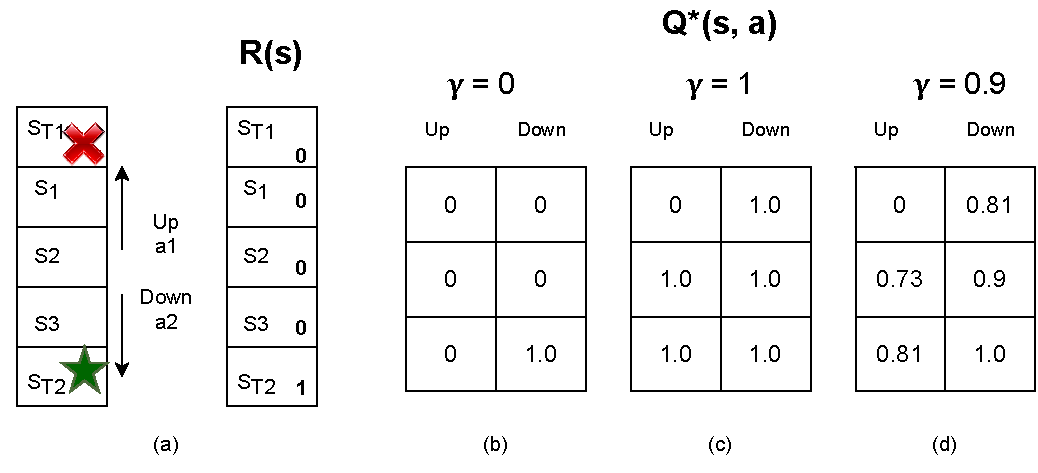
\includegraphics[height=2.5in]{figs/DRL-1d-Q_new}
\caption{
  Left: illustration of a simple MDP
  corresponding to a 1d grid world
  of 3 non-absorbing states and 2 actions.
  Right: optimal $Q$-functions for different values of $\gamma$.
\figbased{Figures 3.1, 3.2, 3.4 of \citep{Graesser2019}}.
}
\label{fig:Q1d}
\end{figure}

\section{Computing the value function and policy given a known world model}
\label{sec:planning}
\label{sec:rl-planning}
\label{sec:DPRL}

In this section, we discuss how
to compute the optimal value function (the \keywordDef{prediction problem})
and the optimal policy (the \keywordDef{control problem})
when the MDP model is known.
(Sometimes the term \keywordDef{planning} is used to refer
to computing the optimal policy, given a known model,
but planning can also refer to computing a sequence of actions,
rather than a policy.)
The algorithms we discuss are based on
\keywordDef{dynamic programming} (DP)
and \keywordDef{linear programming} (LP).

For simplicity, in this section, we assume
discrete state and action sets with $\gamma<1$.
However,
exact calculation of optimal policies often depends
polynomially on the sizes of $\calS$ and $\calA$,
and is intractable, for example, when the state space
is a Cartesian product of several finite sets.
This challenge is known as the
\keywordDef{curse of dimensionality}.
Therefore, approximations are typically needed,
such as using parametric or nonparametric representations of the value function or policy,
both for computational tractability and
for extending the methods to handle MDPs
with general state and action sets.
This requires the use of
\keywordDef{approximate dynamic programming} (ADP)
and \keywordDef{approximate linear programming} (ALP)
algorithms (see e.g., \cite{BertsekasRL}).

\eat{
using \keywordDef{dynamic programming} (\keywordDef{DP}).
The inputs to the algorithm
are the world model $p(s'|s,a)$
and reward function $R(s,a)$,
and the output is the optimal policy and 
its value function.
(This is called  \keywordDef{planning} using a known model.)
We assume the states and actions are discrete,
although similar methods can also be used in the linear-Gaussian case.
%(In fact the state space can be large, as long as $p(s'|s,a)$ is sparse.)
}

\subsection{Value iteration}
\label{sec:valueIter}
\label{sec:VI}

A popular and effective DP method for solving an MDP is
\keywordDef{value iteration} (VI).
Starting from an initial value function estimate $V_0$, the algorithm
iteratively updates the estimate by 
\begin{align}
\label{eqn:value-iteration}
V_{k+1}(s) = \max_a \left[
  R(s,a) + \gamma \sum_{s'} p(s'|s,a) V_k(s') \right]
\end{align}
Note that the update rule, sometimes called a
\keywordDef{Bellman backup},
is exactly the right-hand side of the Bellman optimality equation \cref{eqn:bellmanOptV}, with the unknown $\Vopt$ replaced by the current estimate $V_k$.
A fundamental property of \cref{eqn:value-iteration}
is that the update is a \keywordDef{contraction}:
it can be verified that
\begin{align}
\label{eqn:bellman-contraction}
\max_s |V_{k+1}(s) - \Vopt(s)| \le \gamma \max_s |V_k(s) - \Vopt(s)|
\end{align}
In other words, every iteration will reduce
the maximum value function error
by a constant factor.

$V_k$ will converge to $\Vopt$,
after which an optimal policy can be extracted using \cref{eqn:optPolFromV}.
In practice, we can often terminate VI
when $V_k$ is close enough to $\Vopt$,
since the resulting greedy policy wrt $V_k$
will be near optimal.
Value iteration can be adapted to learn the optimal action-value function $\Qopt$.

\subsection{Real-time dynamic programming (RTDP)}
\label{sec:RTDP}


In value iteration, we compute $\Vopt(s)$ and $\polopt(s)$
for all possible states $s$,
averaging over all possible next states $s'$ at each iteration,
as illustrated in \cref{fig:sutton-8-6}(right).
However, for some problems,
we may only be interested in the value (and policy)
for certain special starting states.
This is the case, for example, in
\keywordDef{shortest path problems} on graphs,
where we are trying to find the shortest
route from the current state to a goal state.
This can be modeled as an episodic MDP
by defining a transition matrix
$\ptran(s'|s,a)$ where
taking edge $a$ from node $s$ leads to the neighboring node $s'$
with probability 1.
The reward function is defined as $R(s,a)=-1$ for all states $s$
except the goal states,
which are modeled as absorbing
states.

In problems such as this, we can use a method
known as \keywordDef{real-time dynamic programming}
or \keywordDef{RTDP} \citep{Barto1995},
to efficiently compute an \keywordDef{optimal partial policy},
which only specifies what to do for the reachable states.
RTDP maintains a value function estimate $V$.
At each step, it performs a Bellman backup for the
current state $s$ by
$V(s) \assign \max_a \expectQ{R(s,a) + \gamma V(s')}{\ptran(s'|s,a)}$.
It picks an action $a$ (often with some exploration), reaches a next state $s'$,
and repeats the process.
%it picks an action $a$ for the current state $s$,
%according to $V$ (e.g., with an $\epsilon$-greedy exploration).
%It then performs a full
%expectation backup
%by computing $V(s) = \expectQ{R(s,a) + \gamma V(s')}{s'  \sim p(s'|s,a)}$.
%It then samples the next state $s'$,
%and repeats the process to update $V(s')$.
This can be seen as a form of the more general
\keywordDef{asynchronous value iteration},
that focuses its computational effort on parts of the state
space that are more likely to be reachable from the current state,
rather than synchronously updating all states at each iteration.
% Sutton p178

\subsection{Policy iteration}
\label{sec:policyIteration}

Another effective DP method for computing $\polopt$ is \keywordDef{policy iteration}.
It is an iterative algorithm that searches in the space
of deterministic policies until converging to an optimal policy.
Each iteration consists of two steps, \keywordDef{policy evaluation} and \keywordDef{policy improvement}.

The policy evaluation step, as mentioned earlier,
computes the value function for the current policy.
Let $\policy$ represent the current policy,
$\vv(s)=\Vpol(s)$ represent the value function encoded as a vector indexed by states,
$\vr(s) = \sum_a \policy(a|s) R(s,a)$ represent the reward vector,
and $\vT(s'|s) = \sum_a \policy(a|s) p(s'|s,a)$ 
represent the state transition matrix.
Bellman's equation for policy evaluation can be
written in the matrix-vector form as
\begin{align}
  \vv &= \vr + \gamma \vT \vv
  \label{eqn:policyEval}
  \end{align}
This is a linear system of equations in $|\cal{S}|$ unknowns.
We can solve it using matrix inversion:
$\vv = (\vI - \gamma \vT)^{-1} \vr$.
Alternatively, we can use value iteration
by computing
$\vv_{t+1} = \vr + \gamma \vT \vv_t$
until near convergence,
or some form of asynchronous variant
that is computationally more efficient.

Once we have evaluated $\Vpol$ for the current policy $\policy$,
we can use it to derive a better policy $\policy'$,
thus the name policy improvement.
To do this, we simply compute a deterministic
policy $\policy'$ that acts greedily with respect to $\Vpol$ in every
state, using
\be
\policy'(s) = \argmax_a \{R(s,a) + \gamma \expect{\Vpol(s')}\}
\ee
We can guarantee that $V_{\policy'} \ge \Vpol$.
This is called the \keywordDef{policy improvement theorem}.
To see this, define $\vr'$, $\vT'$ and $\vv'$ as before,
but for the new policy $\policy'$.
The definition of $\policy'$ implies
$\vr' + \gamma \vT' \vv \ge \vr + \gamma \vT \vv = \vv$,
where the equality is due to Bellman's equation.
Repeating the same equality, we have
\begin{align}
\vv &\le \vr' + \gamma \vT' \vv
\le \vr' + \gamma \vT' (\vr' + \gamma \vT' \vv)
\le \vr' + \gamma \vT' (\vr' + \gamma \vT' (\vr' + \gamma \vT' \vv) ) \le \cdots \\
&= (\vI + \gamma \vT' + \gamma^2 \vT'^2 + \cdots) \vr'
= (\vI - \gamma \vT')^{-1} \vr'
= \vv'
\end{align}

Starting from an initial policy $\policy_0$, policy iteration alternates
between policy evaluation ($E$)
and improvement ($I$) steps,
as illustrated below:
\begin{align}
\policy_0 \stackrel{E}{\ra} V_{\policy_0}
\stackrel{I}{\ra} \policy_1
\stackrel{E}{\ra} V_{\policy_1}
\cdots
\stackrel{I}{\ra} \polopt
\stackrel{E}{\ra} \Vopt
\end{align}
%where $E$ stands for policy evaluation and $I$ stands for policy improvement.
The algorithm stops at iteration $k$, if the policy $\policy_k$
is greedy with respect to its own value function $V_{\policy_k}$.
In this case, the policy is optimal.
Since there are at most $|\calA|^{|\calS|}$ deterministic policies,
and every iteration strictly improves the policy, the algorithm must converge after finite iterations.


%\label{sec:GPI}
In PI,
we alternate between policy evaluation (which involves multiple
iterations, until convergence of $\Vpol$),
and policy improvement.
In VI, we alternate between
one iteration of policy evaluation followed
by one iteration of policy improvement
(the ``$\max$'' operator in the update rule).
%In \keywordDef{generalized policy improvement} or \keywordDef{GPI},
We are in fact free to intermix any number of
these steps in any order.
The process will converge once the
policy is greedy wrt its own  value function.



\begin{figure}
\centering
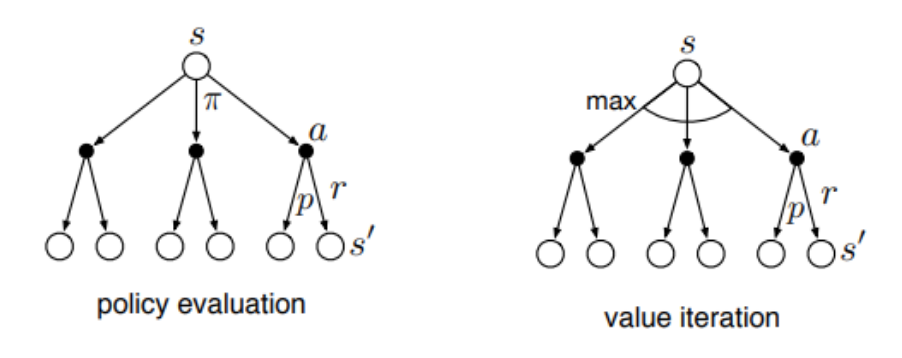
\includegraphics[height=1.5in]{figs/sutton-8-6-PI-VI}
\caption{
  Policy iteration vs value iteration represented as backup diagrams.
  Empty circles represent states, solid (filled) circles
  represent states and actions.
  \figbased{Figure 8.6 of \citep{Suttonv2}}.
}
\label{fig:sutton-8-6}
\end{figure}

Note that policy evaluation computes $\Vpol$
whereas value iteration computes $\Vopt$.
This difference is illustrated in \cref{fig:sutton-8-6},
using a \keywordDef{backup diagram}.
Here the root node represents any state $s$,
nodes at the next level represent state-action combinations
(solid circles),
and nodes at the leaves representing the set of possible
resulting next state $s'$ for each possible action.
In PE, we average over all actions according
to the policy, whereas in VI, we take the maximum over
all actions.

\section{Computing the value function  without knowing the world model}

In the rest of this chapter,
we assume the agent only has  access to samples from
the environment, $(s',r) \sim p(s',r|s,a)$.
We will show how to use these samples
to learn optimal value function and $Q$-function,
even without knowing the MDP dynamics.



\subsection{Monte Carlo estimation}
\label{sec:MCRL}

Recall that $\Vpol(s) = \expect{\return_t | s_t=s}$
is the sum of expected (discounted) returns from state $s$
if we follow policy $\pi$.
A simple way to estimate this is to rollout the policy,
and then compute the average
sum of discounted rewards.  The trajectory ends when we reach a terminal state, if
the task is episodic, or when the discount factor $\gamma^t$ becomes
negligibly small, whichever occurs first.
This is called \keywordDef{Monte Carlo estimation}.
We can use this to update our estimate of the value function as follows:
\begin{align}
\label{eqn:rl-td}
V(s_t) &\assign V(s_t) + \lr
\left[
 \return_t  - V(s_t)
  \right]
\end{align}
where $\lr$ is the learning rate, and the term in brackets is an error term.
We can use a similar technique to estimate
$\Qpol(s,a) = \expect{\return_t | s_t=s,a_t=a}$
by simply starting the rollout with action $a$.

We can use MC estimation of $Q$,  together with policy iteration
(\cref{sec:policyIteration}), to learn an optimal policy.
Specifically,
at iteration $k$,
we compute a new, improved policy using
$\policy_{k+1}(s) = \argmax_a Q_k(s,a)$,
where $Q_k$ is approximated using MC estimation.
This update can be applied to all the states visited
on the sampled trajectory.
This overall technique
is called \keywordDef{Monte Carlo control}.

To ensure this method converges to the optimal policy,
we need to collect data for every (state, action) pair,
at least in the tabular case,
since there is no generalization
across different values of $Q(s,a)$.
One way to achieve this is to use an $\epsilon$-greedy policy
 (see \cref{sec:epsGreedy}).
Since this is an on-policy algorithm,
the resulting method will converge
to the optimal $\epsilon$-soft policy,
as opposed to the optimal policy.
It is possible to use importance sampling
to estimate the value function for the optimal policy,
even if actions are chosen according to the $\epsilon$-greedy policy.
However, it is simpler to just gradually reduce $\epsilon$.
% Sutton p101

\subsection{Temporal difference (TD) learning}
\label{sec:TD}

The Monte Carlo (MC) method in \cref{sec:MCRL}
results in 
an estimator for $V(s)$ with very high variance,
since it has to unroll many trajectories, 
whose returns are a sum of many random rewards generated by stochastic state transitions.
%might yield very different returns.
In addition, it is limited to episodic tasks
(or finite horizon truncation of continuing tasks),
since it must unroll to the end of the episode
before each update step,
to ensure it reliably estimates the long term return.

In this section, we discuss a more efficient technique called
\keywordDef{temporal difference} or \keywordDef{TD} learning
\citep{Sutton88}.
The basic idea is to incrementally
reduce the Bellman error
%, which is the difference between the LHS and RHS of the Bellman equations,
for sampled states or state-actions,
based on transitions instead of a long trajectory.
More precisely, suppose we are to learn
the value function $\Vpol$ for a fixed policy $\policy$.
Given a state transition $(s_t,a_t,r_t,s_{t+1})$,
where $a_t \sim \policy(s_t)$,
we change the estimate $V(s_t)$ so that
it moves towards the  \keywordDef{target value}
$\targetV_t = r_t + \gamma V(s_{t+1}) \approx G_{t:t+1}$:
\begin{align}
V(s_t) &\assign V(s_t) + \lr
\left[
  \underbrace{r_t + \gamma V(s_{t+1}) - V(s_t)}_{\delta_t}
  \right]
%  &= (1-\lr) V(s_t) + \lr \big(r_t + \gamma V(s_{t+1}) \big) \notag
\end{align}
where $\lr$ is the learning rate.
(See \citep{Ryzhov2015} for ways to adaptively set the learning rate.)
The $\delta_t=y_t - V(s_t)$ term 
is known as the \keywordDef{TD error}.
A more general form of TD update
for parametric value function representations is
\begin{align}
\label{eqn:rl-td-approx}
\vw \assign \vw + \lr \left[
r_t + \gamma \Vapprox(s_{t+1})
  - \Vapprox(s_t) \right] \nabla_{\vw}\Vapprox(s_t)
\end{align}
we see that  \cref{eqn:rl-td} is a special case.
The TD update rule for evaluating $\Qpol$ is similar,
except we replace states with states and actions.

% Sutton and Bartoe p202

It can be shown that TD learning in the tabular case,
\cref{eqn:rl-td}, converges to the correct value function,
under proper conditions~\citep{BertsekasRL}.
%such as the the decay schedule of learning rate~\citep{BertsekasRL}.
However, it may diverge when using nonlinear function approximators,
as we discuss in \cref{sec:deadlytriad}.
The reason is that this update is a
``\keywordDef{semi-gradient}'',
which refers to the fact
that we only take the gradient wrt the  value function,
$\nabla_{\vw} V(\vs_t, \vw_t)$,
treating the target $U_t$ as constant.

The potential divergence of TD is also consistent with
the fact that \cref{eqn:rl-td-approx} does not correspond
to a gradient update
on any objective function, despite having
a very similar form to SGD (stochastic gradient descent).
Instead, it is an example of \keywordDef{bootstrapping},
%As mentioned in \cref{sec:rl-introl-valuebased},
%updates like \cref{eqn:rl-td} are based on
%the idea of \keywordDef{bootstrapping},
in which the estimate, $\Vapprox(s_t)$,
is updated to approach a target,
$r_t + \gamma \Vapprox(s_{t+1})$,
which is defined by the value function estimate itself.
This idea is shared by DP methods
like value iteration, although they rely on the
complete MDP model to compute an exact Bellman backup.
In contrast, TD learning can be viewed as using
sampled transitions to approximate such backups.
An example of a non-bootstrapping approach is the
Monte Carlo estimation in the previous section.
It samples a complete trajectory,
rather than individual transitions,
to perform an update;
this avoids the divergence issue,
but is  often much less
efficient.
\cref{fig:TD-MC-DP} illustrates the difference between
MC, TD, and DP.

\begin{figure}
\centering
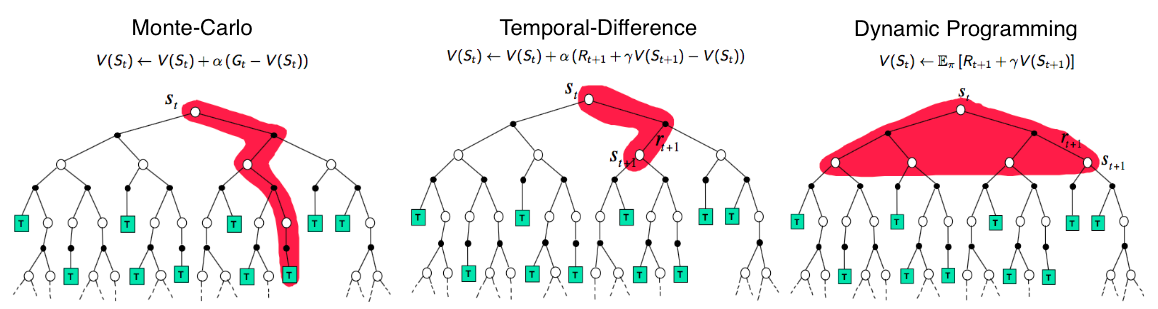
\includegraphics[height=1.5in]{figs/TD-MC-DP-backups}
\caption{
  Backup diagrams of $V(s_t)$ for Monte Carlo,
  temporal difference, and dynamic programming
  updates of the state-value function.
%  \figtaken{a figure from \citep{Silver2018L4}}.
%\figthanks{David Silver}.
\figthanks{Andy Barto}.
}
\label{fig:TD-MC-DP}
\end{figure}



\subsection{Combining TD and MC learning using TD($\lambda$)}
\label{sec:TDlambda}
\label{sec:nstep}

A key difference between TD and MC is
the way they estimate returns.
Given a trajectory
$\traj=(s_0,a_0,r_0,s_1,\ldots,s_T)$,
TD estimates the return from state $s_t$
by one-step lookahead,
$\return_{t:t+1} = r_t + \gamma V(s_{t+1})$,
where the return from time $t+1$ is replaced by
its value function estimate.
In contrast, MC waits until the end of the episode
or until $T$ is large enough,
then uses the estimate
$\return_{t:T} = r_t + \gamma r_{t+1} + \cdots + \gamma^{T-t-1} r_{T-1}$.
It is possible to interpolate between these by
performing an $n$-step rollout, and then using
the value function to approximate the return
for the rest of the trajectory,
similar to heuristic search (\cref{sec:heuristic}).
That is, we can use the \keywordDef{n-step return}
\begin{align}
\return_{t:t+n} = r_{t} + \gamma r_{t+1} + \cdots
+ \gamma^{n-1} r_{t+n-1} + \gamma^n V(s_{t+n})
\end{align}
For example, the 1-step and 2-step returns are given by
\begin{align}
  \return_{t:t+1} &= r_{t} + \gamma v_{t+1} \\
  \return_{t:t+1} &= r_{t} + \gamma r_{t+1} + \gamma^2 v_{t+2} \
  \end{align}
The corresponding $n$-step version of the TD update becomes
\begin{align}
  %V(s_t) \assign V(s_t) + \lr \left[\return_{t:t+n} - V(s_t)\right]
  \vw \assign \vw + \lr
  \left[\return_{t:t+n}  - \Vapprox(s_t) \right]
  \nabla_{\vw}\Vapprox(s_t)
\end{align}

Rather than picking a specific lookahead value, $n$,
we can take a weighted average of all possible values,
with a single parameter $\lambda\in[0,1]$,
by using
\begin{align}
\label{eqn:rl-gamma-return}
\return_{t}^{\lambda}
\defeq (1-\lambda) \sum_{n=1}^{\infty} \lambda^{n-1} \return_{t:t+n}
\end{align}
This is called the \keywordDef{lambda return}.
Note that these coefficients sum to one
(since $\sum_{t=0}^{\infty} (1-\lambda) \lambda^t = \frac{1-\lambda}{1-\lambda}=1$,
for $\lambda<1$),
so the return is a convex combination of $n$-step returns.
See \cref{fig:TDlambda} for an illustration.
We can now use $\return_t^{\lambda}$ inside the TD update
instead of $\return_{t:t+n}$;
this is called \keywordSpecial{TD$(\lambda)$}{TD(lambda)}.

Note that, if a terminal state is entered at step $T$ (as happens with episodic tasks),
then all subsequent $n$-step returns are equal to the conventional return, $G_t$.
Hence we can write
\begin{align}
  G_t^{\lambda} = (1-\lambda) \sum_{n=1}^{T-t-1}
  \lambda^{n-1} G_{t:t+n}
  \;
  + \lambda^{T-t-1} G_t
\end{align}
From this we can see that if $\lambda=1$, the $\lambda$-return
becomes equal to the regular MC return $G_t$.
If $\lambda=0$, the $\lambda$-return becomes equal to the
one-step return $G_{t:t+1}$ (since $0^{n-1}=1$ iff $n=1$),
so standard TD learning is often called
\keywordDef{TD(0) learning}.
This episodic form also gives us the following recursive equation
\be
G_t^{\lambda} = r_t + \gamma[(1-\lambda) v_{t+1} + \lambda G_{t+1}^{\lambda}]
\ee
which we initialize with $G_T=v_t$.
% https://github.com/google-deepmind/rlax/blob/master/rlax/_src/multistep.py#L34

\begin{figure}
\centering
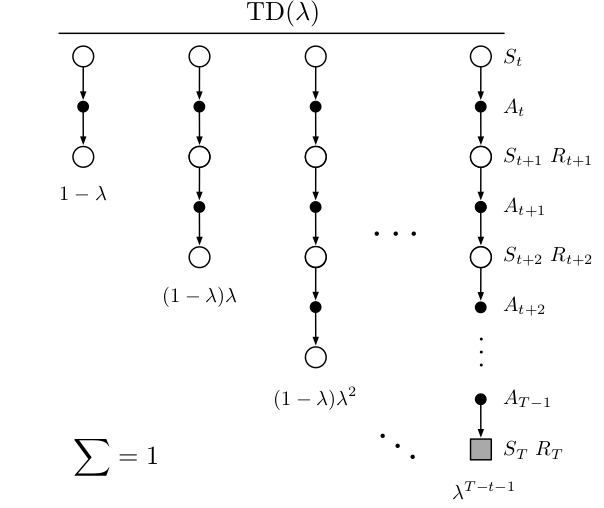
\includegraphics[height=2in]{figs/sutton-12-1}
\caption{
  The backup diagram for TD($\lambda$).
  Standard TD learning corresponds to $\lambda=0$,
  and standard MC learning corresponds to $\lambda=1$.
  \figtaken{Figure 12.1 of \citep{Suttonv2}}.
  \figthanks{Richard Sutton}.
}
\label{fig:TDlambda}
\end{figure}

\subsection{Eligibility traces}
\label{sec:eligibility}


An important benefit of using the geometric weighting
in \cref{eqn:rl-gamma-return}, as opposed to the $n$-step update,
is that
the corresponding TD learning update can be
efficiently implemented  through the use of
\keywordDef{eligibility traces},
even though $\return_{t}^{\lambda}$ is
a sum of infinitely many terms.
The eligibility term is a weighted sum of the gradients
of the value function:
\be
\vz_t = \gamma \lambda \vz_{t-1} + \nabla_{\vw} V_{\vw}(s_t)
\ee
(This trace term gets reset to 0 at the start of each episode.)
We replace the TD(0) update of
$\vw_{t+1} = \vw_t + \lr \delta_t \nabla_{\vw} V_{\vw}(s_t)$
with the TD($\lambda$) version to get
\be
\vw_{t+1} = \vw_t + \lr \delta_t \vz_t
\ee
See \citep{VanSeijen2016} for more details.

\section{SARSA: on-policy TD control}
\label{sec:SARSA}

TD learning is for policy evaluation,
as it estimates the value function for a fixed policy.
In order to find an optimal policy,
we may use the algorithm as a building block inside
generalized policy iteration (\cref{sec:policyIteration}).
In this case, it is more convenient
to work with the action-value function, $Q$, and
a policy $\policy$ that is greedy with respect to $Q$.
The agent follows $\policy$ in every step
to choose actions, and upon a transition $(s,a,r,s')$
the TD update rule is
\begin{align}
Q(s,a) \assign Q(s,a) + \lr \left[ r + \gamma Q(s',a') - Q(s,a) \right]
\label{eqn:rl-td-q}
\end{align}
where $a' \sim \policy(s')$ is the action
the agent will take in state $s'$.
After $Q$ is updated (for policy evaluation),
$\policy$ also changes accordingly as it is greedy
with respect to $Q$ (for policy improvement).
This algorithm, first proposed by \citep{Rummery1994},
was further studied and renamed to
\keywordDef{SARSA} by \citep{Sutton1996};
the name comes from its update rule that
involves an augmented transition $(s,a,r,s',a')$.

In order for SARSA to converge to $\Qopt$,
every state-action pair must be visited infinitely often,
at least in the tabular case,
since the algorithm only updates $Q(s,a)$
for $(s,a)$ that it visits.
One way to ensure this condition is to use a
``greedy in the limit with infinite exploration''
(\keywordDef{GLIE}) policy.
An example is the $\epsilon$-greedy policy,
with $\epsilon$ vanishing to $0$ gradually.
It can be shown that SARSA with a GLIE policy will
converge to $\Qopt$ and $\polopt$~\citep{Singh2000}.


\section{Q-learning: off-policy TD control}
\label{sec:Qlearning}

SARSA is an \keyword{on-policy} algorithm,
which means it learns the $Q$-function for the policy
it is currently using,
which is typically not the optimal policy,
because of the need to perform exploration.
However, with a simple modification,
we can convert this to an \keyword{off-policy}
algorithm that learns $\Qopt$,
even if a suboptimal or exploratory policy is used to choose actions.


\subsection{Tabular Q learning}

Suppose we modify SARSA by replacing the sampled next action
$a' \sim \policy(s')$ in \cref{eqn:rl-td-q}
with a greedy action:
$a' = \argmax_b Q(s',b)$.
This results in the following update
when a transition $(s,a,r,s')$ happens
\begin{align}
Q(s,a) \assign Q(s,a) + \lr \left[
  r + \gamma \max_{a'} Q(s',a') - Q(s,a) \right]
\label{eqn:Qlearning}
\end{align}
This is the update rule of \keywordDef{Q-learning}
for the tabular case~\citep{Watkins92}.


Since it is off-policy,
the method can use  $(s,a,r,s')$ triples
coming from any data source,
such as older versions of the policy,
or log data from an existing (non-RL) system.
If every state-action pair is visited infinitely often,
the algorithm provably converges to $\Qopt$
in the tabular case, with properly decayed learning rates~\citep{BertsekasRL}.
%See \cref{fig:oneStep} for a visual comparison of Q-learning,
%SARSA, TD and DP methods.
\cref{algo:Qlearning} gives a vanilla implementation of
Q-learning
%(with functiion approximation)
with $\epsilon$-greedy exploration.

\begin{algorithm}
\dontprintsemicolon
\caption{Tabular Q-learning with $\epsilon$-greedy exploration}
\label{algo:Qlearning}
Initialize value function $Q$ \\
\Repeat{converged}
       {
       Sample starting state $s$ of new episode \\
       \Repeat{state $s$ is  terminal}
       {
       Sample action
       $a=\begin{cases}
       \argmax_{b} Q(s,b), & \text{with probability $1-\epsilon$} \\
       \text{random action}, & \text{with probability $\epsilon$}
       \end{cases}$
               \\
       $(s',r) = \text{env.step}(a)$ \\
       Compute the TD error: $\delta = r + \gamma \max_{a'} Q(s',a') - Q(s,a)$ \\
       $Q(s,a) \leftarrow Q(s,a) + \lr \delta$ \\
       $s \leftarrow s'$ 
         }
}
\end{algorithm}

\eat{
\begin{algorithm}
\dontprintsemicolon
\caption{Q-learning with $\epsilon$-greedy exploration}
\label{algo:Qlearning}
Initialize value function parameters $\vw$ \\
\Repeat{converged}
       {
       Sample starting state $s$ of new episode \\
       \Repeat{state $s$ is  terminal}
       {
       Sample action
       $a=\begin{cases}
       \argmax_{b} \Qapprox(s,b), & \text{with probability $1-\epsilon$} \\
       \text{random action}, & \text{with probability $\epsilon$}
       \end{cases}$
               \\
       Observe state $s'$, reward $r$ \\
       Compute the TD error: $\delta = r + \gamma \max_{a'} \Qapprox(s',a') - \Qapprox(s,a)$ \\
       $\vw \assign \vw + \lr \delta \nabla_{\vw} \Qapprox(s,a)$ \\
           $s \assign s'$
         }
}
\end{algorithm}
}


%\subsection{Done states}
%\label{sec:done}

For terminal states, $s \in \calS^+$, we know that
$Q(s,a)=0$ for all actions $a$.
Consequently, for the optimal value function,
we have
$V^*(s) = \max_{a'} Q^*(s,a)=0$
for all terminal states.
%
When  performing online learning, we don't usually know
which states are terminal.
Therefore we assume that, whenever we take a step in the environment,
we get the next state $s'$ and reward $r$,
but also a binary indicator $\done(s')$ that tells us
if $s'$ is terminal.
In this case,  we set the target value in Q-learning
to $V^*(s')=0$ yielding the modified update rule:
\begin{align}
Q(s,a) \assign Q(s,a) + \lr \left[
  r + (1-\done(s')) \gamma \max_{a'} Q(s',a') - Q(s,a) \right]
\label{eqn:Qlearningdone}
\end{align}
For brevity, we will usually ignore this factor in the subsequent equations,
but it needs to be implemented in the code.

%\subsection{Example}
%\label{sec:Qlearning1d}


\begin{figure}
\centering
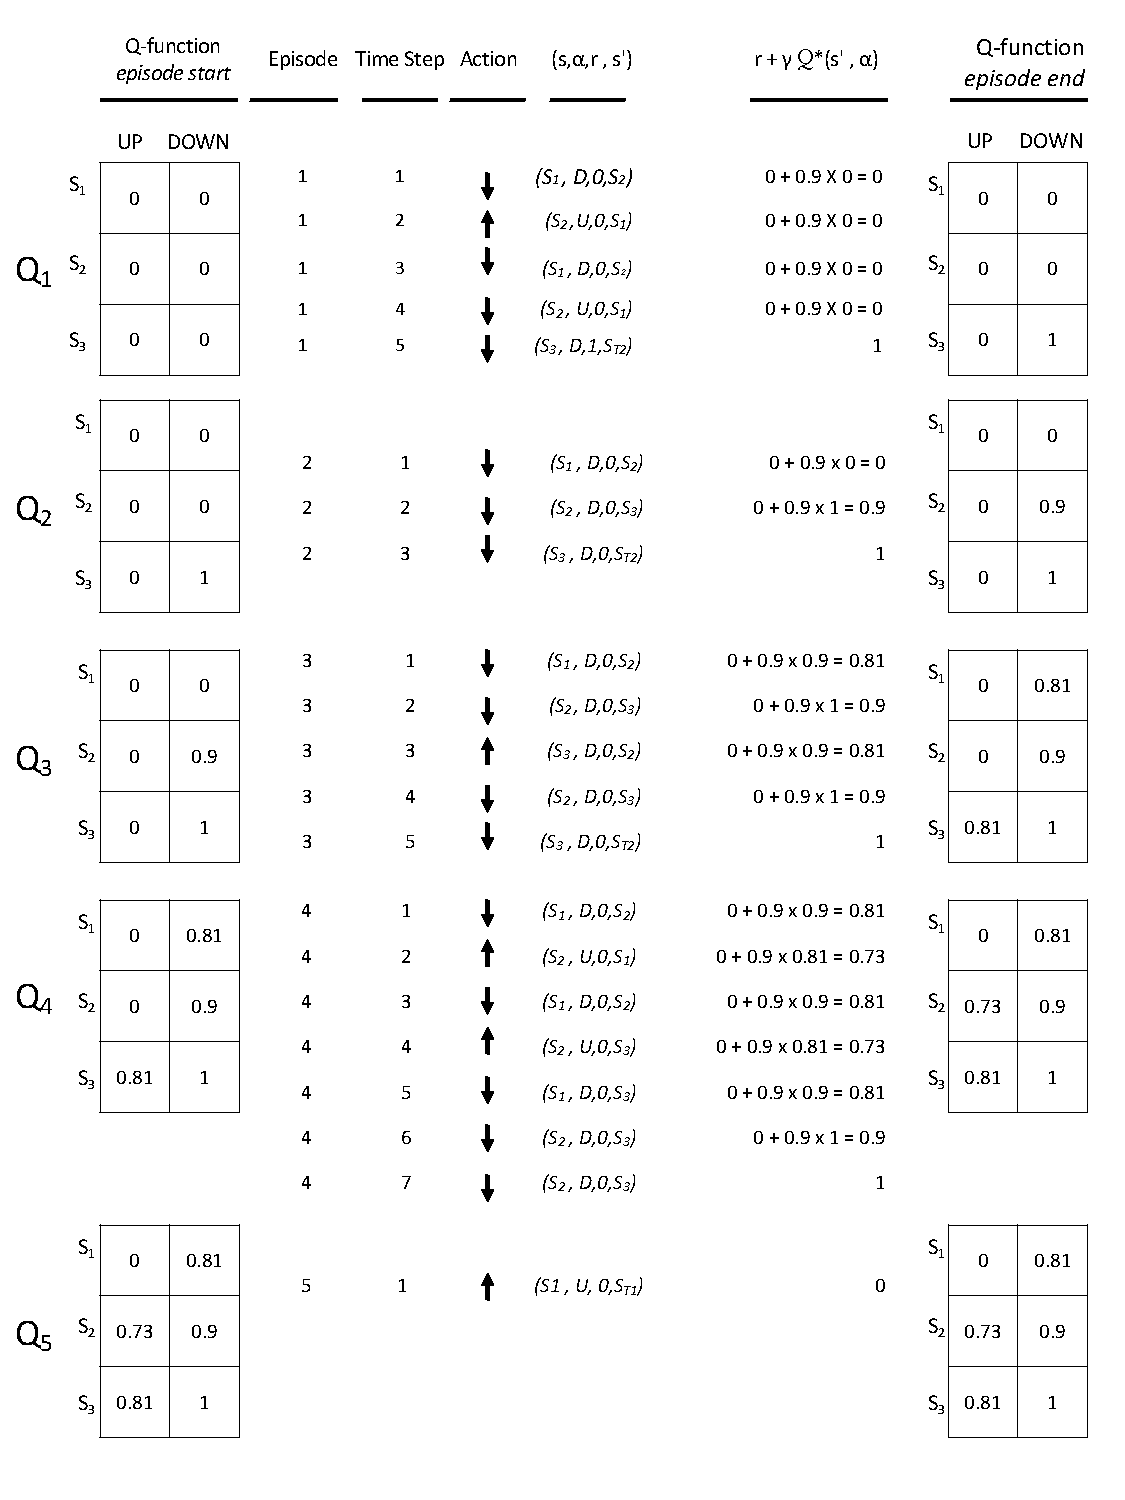
\includegraphics[height=5in]{figs/DRL-3-3}
\caption{
  Illustration of Q learning for one random trajectory
  in the 1d grid world
  in \cref{fig:Q1d} using $\epsilon$-greedy exploration.
  At the end of episode 1, we make a transition
  from $S_3$ to $S_{T2}$ and get a reward of $r=1$,
  so we estimate $Q(S_3,\downarrow)=1$.
  In episode 2, we make a transition from $S_2$ to $S_3$,
  so $S_2$ gets incremented by $\gamma Q(S_3,\downarrow)=0.9$.
  \figbased{Figure 3.3 of \citep{Graesser2019}}.
}
\label{fig:DRLTD}
\end{figure}

\cref{fig:DRLTD} gives an example
of Q-learning applied to the simple 1d grid world
from \cref{fig:Q1d}, using $\gamma=0.9$.
We show the $Q$-functon at the start and end of each episode,
after performing actions chosen by an $\epsilon$-greedy policy.
We initialize $Q(s,a)=0$ for all entries,
and use a step size of $\lr=1$.
At convergence, we have
$\Qopt(s,a) = r + \gamma \Qopt(s',a_*)$,
where $a_* = \downarrow$ for all states.




\subsection{Q learning with function approximation}
\label{sec:Qfn}

To make Q learning work with high-dimensional state spaces,
we have to replace the tabular (non-parametric) representation
with a parametric approximation, denoted $Q_{\vw}(s,a)$.
We can update this function using one or more steps of SGD
on the following loss function
\begin{align}
  \loss(\vw|\vs,a,r,\vs') &=
  \big( (r + \gamma \max_{a'} Q_{\vw}(\vs',a')) -   Q_{\vw}(\vs,a) \big)^2  
  \label{eqn:ynaive}
\end{align}
Since nonlinear functions need to be trained on minibatches
of data, we compute the average loss over multiple
randomly sampled
experience tuples (see \cref{sec:ER} for discussion)
  to get
  \begin{align}
\loss(\vw) &= \expectQ{\loss(\vw|\vs,a,r,\vs')}{(\vs,a,r,\vs') \sim U(\data)}
  \end{align}
%The random sampling helps reduce correlation between the samples.
%\begin{align}
%\vw  \assign \vw + \lr \left[
%  r + \gamma \max_{a'} Q_{_\vw}(s',a') - Q_{\vw}(s,a) \right]
%\nabla_{\vw} Q_{\vw}(s,a)
%\end{align}
See \cref{algo:Qfn} for the pseudocode.


\begin{algorithm}
\dontprintsemicolon
\caption{Q learning with function approximation and replay buffers}
\label{algo:Qfn}
Initialize environment state $\vs$,
network parameters $\vw_0$,
replay buffer $\data=\emptyset$,
discount factor $\gamma$,
step size $\eta$,
policy
$\pi_0(a|s) = \epsilon \text{Unif}(a)
+ (1-\epsilon) \delta(a=\argmax_a Q_{\vw_0}(s,a))$ \\
\For{iteration $k=0,1,2,\ldots$}
    {
      \For{environment step $s=0,1,\ldots,S-1$}
          {
            Sample action: $a \sim \pi_k(a|s)$ \\
            Interact with environment: $(s',r) = \text{env.step}(a)$ \\
            Update buffer: $\data \leftarrow \data \union \{ (s,a,s',r) \}$ 
          }
          $\vw_{k,0} \leftarrow \vw_k$ \\
          \For{gradient step $g=0,1,\ldots,G-1$}
              {
                Sample batch: $B \subset \data$ \\
                Compute error: $\loss(B,\vw_{k,g})
                = \frac{1}{|B|} \sum_{(s,a,r,s') \in B}
                \left[ Q_{\vw_{k,g}}(s,a) - (r + \gamma \max_{a'} Q_{\vw_k}(s',a')) \right]^2$\\
                Update parameters:
                $\vw_{k,g} \leftarrow \vw_{k,g} - \lr \nabla_{\vw_{k,g}}
                \loss(B,\vw_{k,g})$
              }
         $\vw_{k+1} \leftarrow \vw_{k,G}$ 
      }
\end{algorithm}

\subsubsection{Neural fitted Q}
\label{sec:NFQ}

The first approach of this kind
is known as \keywordDef{neural fitted Q iteration}
\citep{Riedmiller2005}, which corresponds to fully optimizing
$\loss(\vw)$ at each iteration (equivalent to using $G=\infty$
gradient steps).

\subsubsection{DQN}
\label{sec:DQN}

The influential
\keyword{deep Q-network} or \keyword{DQN}
paper of \citep{Mnih2015atari}
also used neural nets to represent the $Q$ function,
but performed a smaller number of gradient updates
per iteration.
Furthermore, they proposed to modify the target value
when fitting the $Q$ function in order to avoid
instabilities during training (see \cref{sec:deadly} for details).

The DQN method became famous since it was able  to train
agents that can outperform
humans when playing various Atari games from
the \keywordDef{ALE} (Atari Learning Environment)
benchmark \citep{Bellemare13}.
Here the input is a small color image,
and the action space corresponds to moving left, right, up or down,
plus an optional shoot action.\footnote{
%
For more discussion of ALE,
see \citep{Machado2018},
and for a recent extension to continuous actions
(representing joystick control),
see the CALE benchmark of \citep{Farebrother2024CALE}.
Note that DQN was not the first deep RL method to train
an agent from pixel input;
that honor goes to \citep{Lange2010},
who trained an autoencoder to embed images into low-dimensional latents,
and then used neural fitted Q learning (\cref{sec:NFQ})
to fit the $Q$ function.
}

Since 2015, many more extensions to DQN have been proposed,
with the goal of
improving performance in various ways,
either in terms of peak reward obtained,
or sample efficiency (e.g., reward obtained after only 100k steps
in the environment, as proposed in the \keywordDef{Atari-100k} benchmark
\citep{Atari100k}),
or training stability,
or all of the above.
We discuss some of these extensions in \cref{sec:DQNextensions}.



\eat{
\subsubsection{DQN}
\label{sec:DQN}


In this section, we discuss the seminal
\keywordDef{deep Q-network} or \keywordDef{DQN}
paper \citep{Mnih2015atari}.
The starting point is to consider the update
for the Q network parameters $\vw$
shown in \cref{algo:Qlearning}.
The gradient update corresponds to taking the gradient
of the following loss
\begin{align}
  \loss(\vw|\vs,a,r,\vs') &=
  \big( (r + \gamma \max_{a'} Q_{\vw}(\vs',a')) -   Q_{\vw}(\vs,a) \big)^2  
  \label{eqn:ynaive}
\end{align}
Since neural nets work best when trained on minibatches
of data, we compute the average loss by sampling
experience tuples (e.g., uniformly at random)
from
  the replay buffer $\data$
  (see \cref{sec:ER})
  to get
  \begin{align}
\loss(\vw) &= \expectQ{\loss(\vw|\vs,a,r,\vs')}{(\vs,a,r,\vs') \sim U(\data)}
  \end{align}
The random sampling helps reduce correlation between the samples.


\begin{algorithm}
\dontprintsemicolon
\caption{DQN (with target network)}
\label{algo:DQNtarget}
Initialize environment state $\vs$,
network parameters $\vw$,
target parameters $\overline{\vw} = \stopgrad(\vw)$,
replay buffer $\data=\emptyset$,
discount factor $\gamma$,
EMA rate $\rho$,
step size $\eta$
\\
\Repeat{converged}
       {
         Take action $a \sim \text{eps-greedy}(\vw)$\\
         $(\vs',r) = \text{step}(a, \vs)$ \\
         $\data := \data \union
         \{ (\vs, a, r, \vs') \}$ \\
         $\vs \assign \vs'$ \\
         Sample a minibatch $\calB = \{(\vs_j,a_j,r_j,\vs'_j)\}$
         from $\data$ \\
           $(\vw,\overline{\vw}) = \text{update}(\vw, \overline{\vw}, \calB)$
        }
.\\
$\text{def update}(\vw,\overline{\vw},\calB)$: \\
       Let $(\vs_j,a_j,r_j,\vs'_j)_{j=1}^B = \calB$ \\
$\targetV_{j} = \TargetV(r_j, \vs'_j; \overline{\vw})$ for $j=1:B$ \\
      $\loss(\vw) = \frac{1}{|\calB|} \sum_{(\vs_j, a_j, r_j, \vs'_j) \in
        \calB} (Q_{\vw}(\vs_j,a_j) - \stopgrad(\targetV_j))^2$\\
      $\vw \assign \vw - \lr_{\vw} \nabla \loss(\vw)$ // Gradient descent step \\
      $\overline{\vw} := \rho \overline{\vw} 
      + (1-\rho) \vw$       //EMA for  target network \\
    Return $\vw, \overline{\vw}$\\
\end{algorithm}
}


\subsubsection{Experience replay}
\label{sec:ER}
\label{sec:replay}

Since Q learning is an off-policy method, we can update the Q function
using any data source. This is particularly important when we use
nonlinear function approximation (see \cref{sec:Qfn}), which often needs a lot of data
for model fitting.
A natural source of data is data collected earlier in the trajectori
of the agent; this is called 
an \keywordDef{experience replay} buffer,
which stores  $(s,a,r,s')$ transition tuples into a buffer.
This can improve the stability and sample efficiency of learning,
and was
originally proposed in \citep{Lin1992}.

This modification has two advantages.
First, it improves data efficiency as every transition
can be used multiple times.
Second, it improves stability in training,
by reducing the correlation of the data samples
that the network is trained on,
since the training tuples do not have to come from
adjacent moments in time.
(Note that experience replay requires the use
of off-policy learning methods, such as Q learning,
since the training data is sampled from older
versions of the policy, not the current policy.)

%\subsubsection{Prioritized experience replay}
\label{sec:PER}

It is possible to replace the uniform sampling
from the buffer
with one that favors more
important transition tuples
that may be more informative about $Q$.
This idea is formalized in 
\citep{Schaul2016},
who develop a technique known as
\keywordDef{prioritized experience replay}.

\eat{
For example, we can sample transitions from $\data$
with probability
$p(s,a,r,s') \propto (|\delta| + \varepsilon)^{\eta}$,
%$p(i) = \frac{(|\delta_i| + \epsilon)^{\eta}}{(\sum_j |\delta_j|+\epsilon)^{\eta}}$,
where $\delta$ is the corresponding TD error
(under the current $Q$-function),
$\varepsilon > 0$ a hyperparameter
to ensure every experience is chosen
with nonzero probability,
and $\eta \geq 0$ controls the ``inverse temperature''
of the distribution (so $\eta=0$ corresponds to uniform sampling).
% Graesser p1110
}

\eat{
Consider the TD error for the $i$'th tuple $\tau_i$
\be
\delta_i = r_i + \gamma \max_{a'} Q_{\overline{\vw}}(s'_i, a')
 - Q_{\vw}(s_i,a_i)
\ee
Define the priority of $i$ as
\be
p_i = (\delta_i + \epsilon)^{\alpha}
\ee
where $\alpha \geq 0$ determines the degree of prioritization,
with $\alpha=0$ corresponding to no prioritization (uniform sampling).
Now define the probability of sampling $i$ as
\be
P(i) = \frac{p_i}{\sum_k p_k}
\ee
Sampling from this distribution will introduce bias relative
to the uniform distribution over the past $M$ samples in the replay buffer.
But we can correct this using importance sampling, as follows:
\begin{align}
  \expectQ{\loss(\tau)}{\text{Uniform}(\tau)}
  &= \sum_{i=1}^M \frac{1}{M} \loss(\tau_i) \\
  &= \sum_{i=1}^M P(\tau_i) \frac{1}{M P(\tau_i)} \loss(\tau_i) \\
  &= \expectQ{w(\tau) \loss(\tau)}{P(\tau)} 
  \end{align}
where we define the importance weight as
\be
w(\tau) = \left(\frac{1}{M P(\tau)} \right)^{\beta(t)}
\ee
Here $\beta(t)$ is a hyperparameter than starts off slightly larger than
0, to ensure that important experiences are not down-weighted too much,
and then is gradually increased to 1,
which results in an unbiased estimate.

%A distributed version of PER,
%known as \keywordDef{APE-X},
%is described in \citep{Horgan2018}.
}


\eat{
\subsubsection{Word of caution}

Unfortunately, when the function is nonlinear,
Q learning can become unstable; see \cref{sec:deadly} for details
of the problem and some solutions.
}






\subsubsection{The deadly triad}
\label{sec:offpolicyrl-deadlytriad}
\label{sec:deadlytriad}
\label{sec:deadlyTriad}
\label{sec:deadly}



\begin{figure}
\centering
\begin{subfigure}[b]{0.55\textwidth}
\centering
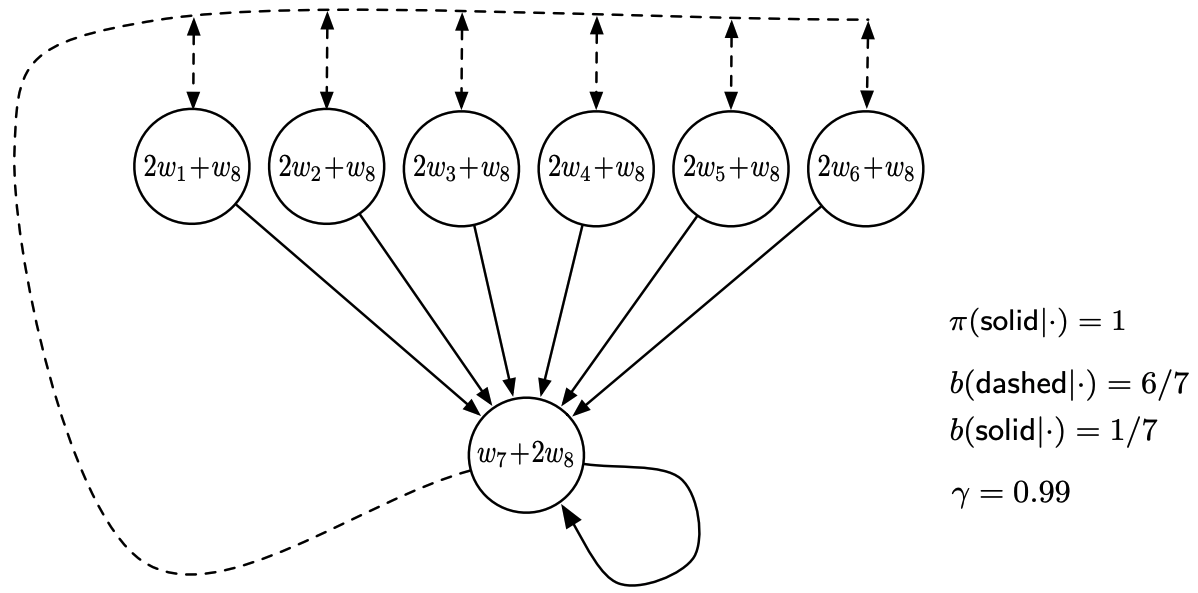
\includegraphics[height=1.75in]{figs/bairdExample}
\caption{ }
\label{fig:baird-example-mdp}
\end{subfigure}
~
\begin{subfigure}[b]{0.35\textwidth}
\centering
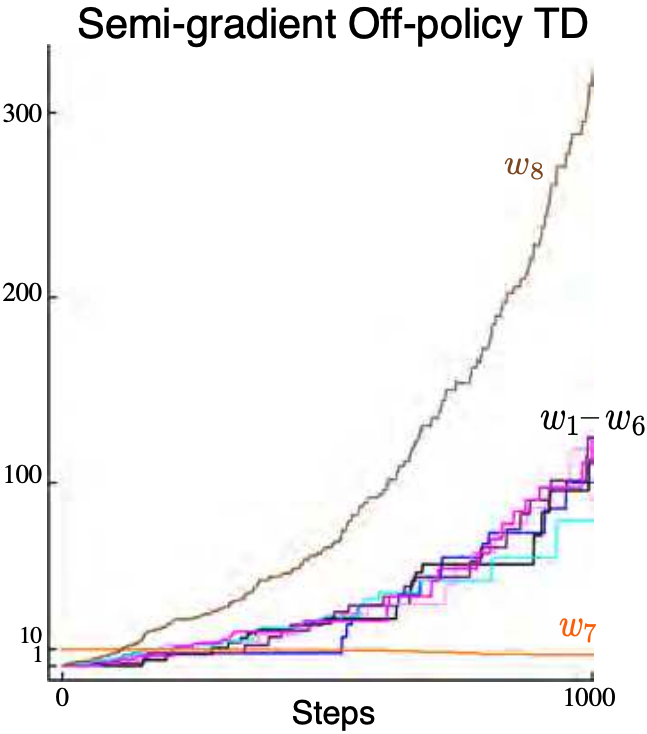
\includegraphics[height=1.75in]{figs/bairdExampleDivergence}
\caption{ }
\label{fig:baird-example-divergence}
\end{subfigure}
\caption{
(a) A simple MDP.
  (b) Parameters of the policy diverge over time.
\figtaken{Figures 11.1 and 11.2 of \citep{Suttonv2}}.
\figthanks{Richard Sutton}.
}
\label{fig:baird-example}
\end{figure}



The problem with the naive Q learning  objective in \cref{eqn:ynaive}
  is that it can lead to instability,
since the target we are regressing towards
uses the same parameters $\vw$ as the function we are updating.
So the network is ``chasing its own tail''.
Although this is fine for tabular models,  it can fail
for nonlinear models, as we discuss below.

In general, an RL algorithm can become unstable when it has
these three components:
function approximation (such as neural networks),
bootstrapped value function estimation (i.e., using TD-like methods instead of MC),
and off-policy learning (where the actions are sampled from some distribution
other than the policy that is being optimized).
This combination is known as \keywordDef{the deadly triad}
\citep{Sutton2015, Vanhasselt18}).
%It highlights another important challenge introduced by off-policy learning,
%and is a subject of ongoing research
%(e.g., \citep{Vanhasselt18,Kumar19}).

A classic example of this is the simple MDP depicted
in \cref{fig:baird-example-mdp}, due to \citep{Baird95}.
(This is known as \keywordDef{Baird's counter example}.)
It has 7 states and 2 actions.
Taking the dashed action takes the environment
to the 6 upper states uniformly at random,
while the solid action takes it to the bottom state.
The reward is 0 in all transitions,
and $\gamma=0.99$.
The value function $\Vapprox$ uses
a linear parameterization indicated by the expressions
shown inside the states, with $\vw\in\real^8$.
The target policies $\policy$ always chooses the
solid action in every state.
Clearly, the true value function, $\Vpol(s) = 0$,
can be exactly represented by setting $\vw=\vzero$.

Suppose we use a behavior policy $b$ to generate
a trajectory,
which chooses the dashed and solid actions
with probabilities $6/7$ and $1/7$, respectively,
in every state.
If we apply TD(0) on this trajectory,
the parameters diverge to $\infty$
(\cref{fig:baird-example-divergence}),
even though the problem appears simple.
In contrast, with on-policy data
(that is, when $b$ is the same as $\policy$),
TD(0) with linear approximation can be guaranteed to
converge to a good value function approximate~\citep{Tsitsiklis97}.
The difference is that with on-policy learning,
as we improve the value function, we also improve the policy,
so the two become self-consistent,
whereas with off-policy learning,
the behavior policy may not match the optimal
value function that is being learned,
leading to inconsistencies.


The divergence behavior is demonstrated in
many value-based bootstrapping methods, including TD, Q-learning,
and related approximate
dynamic programming algorithms,
where the value function is represented
either linearly (like the example above)
or nonlinearly~\citep{Gordon95,Tsitsiklis1997,Ostrovski2021}.
The root cause of these divergence phenomena
is that bootstrapping methods
typically are not minimizing a fixed objective function.  Rather, they
create a learning target using their own estimates, thus potentially
creating a self-reinforcing loop to push the estimates to infinity.
%In certain special cases, such a loop is not possible if data is
%on-policy, so one way to fix the problem is to apply off-policy
%correction methods discussed earlier.  
More formally, the problem is that
the contraction property in the tabular case
(\cref{eqn:bellman-contraction})
may no longer hold when $V$ is approximated by $\Vapprox$.

We discuss some solutions to the deadly triad problem below.


\subsubsection{Target networks}
\label{sec:targetNetwork}

One heuristic solution to the deadly triad,
proposed in the DQN paper,
is to use a  ``frozen'' 
\keywordDef{target network} computed at an earlier iteration
to define the target value for the DQN updates,
rather than trying to chase a constantly moving target.
Specifically, we maintain an extra copy
the $Q$-network, $Q_{\vw^-}$, 
with the same structure as $\Qapprox$.
This new $Q$-network is used
to compute bootstrapping targets
\be
\TargetV(r,\vs'; \vw^{-}) = r + \gamma \max_{a'} Q_{\vw^-}(\vs',a')
\ee
for training $\Qapprox$.
We can periodically set $\vw^{-} \assign \stopgrad(\vw)$,
usually after a few episodes,
where the stop gradient operator
is used to prevent autodiff propagating gradients back to $\vw$.
Alternatively, we can use
an exponential moving average (EMA)
of the weights,
i.e.,
we use 
 $\overline{\vw} = \rho \overline{\vw} + (1-\rho) \stopgrad(\vw)$,
where 
$\rho \ll 1$ ensures that $Q_{\overline{\vw}}$ slowly catches
up with $Q_{\vw}$.
(If $\rho=0$, we say that this is a \keywordDef{detached target},
since it is just a frozen copy of the current weights.)
The final loss  has the form
  \begin{align}
    \loss(\vw) &= \expectQ{\loss(\vw|\vs,a,r,\vs')}{(\vs,a,r,\vs') \sim U(\data)} \\
      \loss(\vw|\vs,a,r,\vs') &=
  (\TargetV(r,\vs';\overline{\vw}) -   Q_{\vw}(\vs,a))^2  
  \end{align}
%See \cref{algo:DQN} for the pseudocode.
Theoretical work justifying this technique is given
in  \citep{Fellows2023,Che2024}.


\eat{
\begin{algorithm}
\dontprintsemicolon
\caption{DQN (with target network)}
\label{algo:DQN}
Initialize environment state $\vs$,
network parameters $\vw$,
target parameters $\overline{\vw} = \stopgrad(\vw)$,
replay buffer $\data=\emptyset$,
discount factor $\gamma$,
EMA rate $\rho$,
step size $\eta$
\\
\Repeat{converged}
       {
         Take action $a \sim \text{eps-greedy}(\vw)$\\
         $(\vs',r) = \text{step}(a, \vs)$ \\
         $\data := \data \union
         \{ (\vs, a, r, \vs') \}$ \\
         $\vs \assign \vs'$ \\
         Sample a minibatch $\calB = \{(\vs_j,a_j,r_j,\vs'_j)\}$
         from $\data$ \\
           $(\vw,\overline{\vw}) = \text{update}(\vw, \overline{\vw}, \calB)$
        }
.\\
$\text{def update}(\vw,\overline{\vw},\calB)$: \\
       Let $(\vs_j,a_j,r_j,\vs'_j)_{j=1}^B = \calB$ \\
$\targetV_{j} = \TargetV(r_j, \vs'_j; \overline{\vw})$ for $j=1:B$ \\
      $\loss(\vw) = \frac{1}{|\calB|} \sum_{(\vs_j, a_j, r_j, \vs'_j) \in
        \calB} (Q_{\vw}(\vs_j,a_j) - \stopgrad(\targetV_j))^2$\\
      $\vw \assign \vw - \lr_{\vw} \nabla \loss(\vw)$ // Gradient descent step \\
      $\overline{\vw} := \rho \overline{\vw} 
      + (1-\rho) \vw$       //EMA for  target network \\
    Return $\vw, \overline{\vw}$\\
\end{algorithm}
}

\subsubsection{Two time-scale methods}

A general way to ensure convergence in off-policy
learning is to construct an objective function,
the minimization of which leads to a good value function approximation.
This is the basis of the
\keywordDef{gradient TD method} of \citep{Sutton2008,Maei2009,Ghiassian2020}.
%https://github.com/rlai-lab/Regularized-GradientTD
%see \citep[Ch.~11]{Suttonv2} for more information.
In practice, this can be achieved by  updating the target value in the TD update
more quickly than the value function itself;
this is known as a \keywordDef{two timescale optimization}
(see e.g., \citep{Yu2017TD,Zhang2019timescale,Hong2023}).
It is also possible to use a standard single timescale
method provided the target value is computed using a 
frozen \keyword{target network},
as discussed in \cref{sec:targetNetwork}.
See \citep{Fellows2023,Che2024} for details.

\subsubsection{Layer norm}

More recently, \citep{PQN} proved that just adding LayerNorm
\citep{Ba2016}
to the penultimate layer of the critic network,
just before the linear head,
is sufficient  to provably yield convergence of TD learning
even in the off-policy setting.
In particular, suppose the network has the form
$Q(s,a|\vw,\vtheta) = \vw^T \relu(\text{LayerNorm}(f(s,a;\vtheta)))$.
Since $||\text{LayerNorm}(f(s,a;\vtheta))|| \leq 1$, we have
$||Q(s,a|\vw,\vtheta) \leq ||\vw||$,
which means the magnitude of the output is always bounded,
as shown in \cref{fig:layerNorm}.
In \citep{PQN}, they prove this (plus $\ell_2$ regularization on $\vw$,
and a sufficiently wide penultimate layer)
is sufficient to ensure convergence 
of the value function estimate.



\begin{figure}
\centering
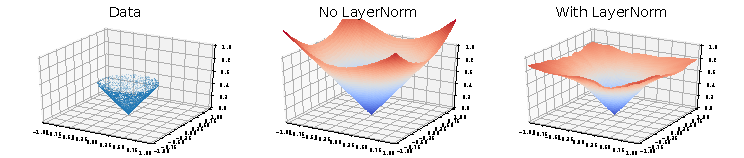
\includegraphics[height=1.5in]{figs/LayerNormFigure}
\caption{
  We generate a dataset (left) with inputs $\vx$
  distributed in a circle with radius 0.5 and labels $y = ||\vx||$.
  We then fit a two-layer MLP without LayerNorm (center)
  and with LayerNorm (right).
  LayerNorm bounds the values and prevents catastrophic overestimation
  when extrapolating.
  \figtaken{Figure  3 of \citep{Ball2023}}.
  \figthanks{Philip Ball}.
}
\label{fig:layerNorm}
\end{figure}



\eat{
% Bo Dai

  Thanks for asking! First, the deadly triad is offpolicy data + general function + TD. We can break the deadly triad by either use optimization based method to replace TD (e.g., LP-based RL with primal-dual solver https://arxiv.org/pdf/2001.01866), or use overparametrized general function (https://arxiv.org/abs/2405.21043). Second, linear value function with appropriate basis is also powerful. We had a series of work on developing the appropriate linear basis (representation) for RL (https://arxiv.org/pdf/2208.09515). Third, for convex Q function, I do not have general answer for general dynamics. However, for the multi-stage stochastic optimization  dynamic problem (https://arxiv.org/pdf/2112.00874), the Q is proved to be convex and TD converges.

 % Tom Zahavy.
  We had this paper on convex RL: https://openreview.net/pdf?id=ELndVeVA-TR, in this case we focus on value functions that are convex in the occupancy (while the value function is linear in it). These functions are quite popular for exploration/diversity/imitation so this convex setting is actually rich and meaningful. The problems are almost equivalent in terms of hardness results.

%  Hado van Hasselt.
  TD with linear value functions also suffers from the deadly triad in the off-policy case, though gradient TD (GTD) algorithms exist that do converge (in addition to alternatives Bo Dai mentioned above).

  Non-linear TD can additionally diverge even in the *on-policy* case. See, e.g., this classic paper by John Tsitsiklis and  @Benjamin Van Roy.
[Tsitsiklis1997]
  I conjecture that convexity in the parameters will not be sufficient to avoid this divergence.  If useful, I could try to construct a simple example to demonstrate this.  (I haven't checked carefully, maybe the example in the paper above is already convex.)

  However, for some problems even non-linear TD is guaranteed to converge.  For instance, this paper by Yann Ollivier
[Ollivier2018]
  that shows non-linear TD converges when the MDP is reversible, because then TD can be interpreted as stochastic gradient descent on a different objective (and therefore then inherits standard convergence properties of SGD).

Strict divergence does not always seem to happen, btw, when using a different optimiser, like ADAM, because this bounds the parameter updates.  This doesn't solve the issue, because the values can still get increasingly inaccurate when using an unstable update (we've called this phenomenon 'soft divergence' in the past).
}



\subsection{Maximization bias}

\begin{figure}
\centering
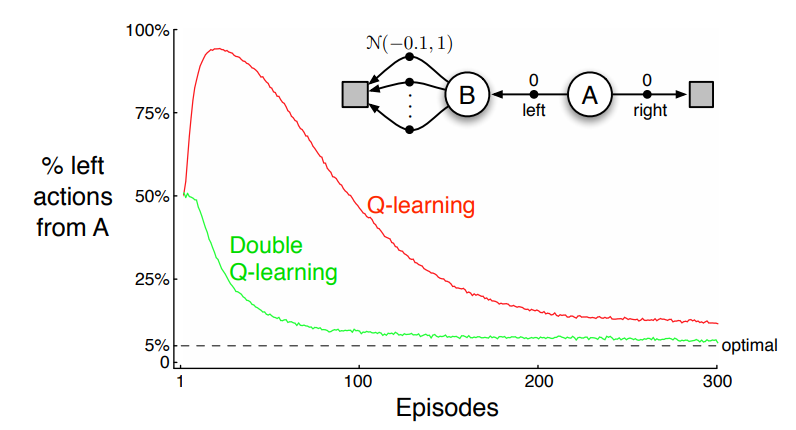
\includegraphics[height=1.5in]{figs/sutton-6-5}
\caption{
  Comparison of Q-learning and double Q-learning on a simple episodic
  MDP using $\epsilon$-greedy action selection with $\epsilon=0.1$.
  The initial state is A, and squares denote absorbing states.
The data are averaged over 10,000 runs.
\figtaken{Figure 6.5 of \citep{Suttonv2}}.
\figthanks{Richard Sutton}.
}
\label{fig:sutton-6-5}
\end{figure}

Standard Q-learning suffers from a problem
known as the \keywordDef{optimizer's curse} \citep{Smith2006},
or the \keywordDef{maximization bias}.
The problem refers to the simple statistical inequality:
$\expect{\max_a X_a} \geq \max_a \expect{X_a}$,
for a set of random variables $\{X_a\}$.
%where $r_i \sim p(R)$ are samples of $R$.
Thus, if we pick actions greedily according to their random scores $\{X_a\}$, we might pick a wrong action just because random noise makes it appealing.

% p135
\cref{fig:sutton-6-5} gives a simple example
of how this can happen in an MDP.
The start state is A.
The right action gives a reward 0 and terminates the episode.
The left action also gives a reward of 0,
but then enters state B,
from which there are many possible actions,
with rewards drawn from $\gauss(-0.1, 1.0)$.
Thus the expected return for any trajectory starting with the left
action is $-0.1$, making it suboptimal.
Nevertheless, the RL algorithm may pick   the left action
due to the maximization bias making B appear to have a positive value.

\subsubsection{Double Q-learning}
\label{sec:double}

One solution to avoid the maximization bias is to
use two separate $Q$-functions, $Q_1$ and $Q_2$,
one for selecting the greedy action,
and the other for estimating the corresponding $Q$-value.
%$\argmax_a Q_1(s,a)$,
%and the other of which is used to estimate the value
%of the chosen action, $Q_2(s,a_*)$.
%This estimate is unbiased,
%since $\expect{Q_2(s,a_*)}=Q(s,a_*)$.
%At each step, we perform the following update
In particular, upon seeing a transition $(s,a,r,s')$,
we perform the following update for $i=1:2$:
\begin{align}
  Q_i(s,a) &\assign Q_i(s,a) + \lr(\targetV_i(s,a) - Q_i(s,a)) \\
  \targetV_i(s,a) &= r + \gamma Q_{i}(s', \argmax_{a'} Q_{-i}(s', a'))
  \label{eqn:doubleQ}
%Q_1(s,a) \assign Q_1(s,a) + \lr \left[
%  r + \gamma Q_2\big(s', \argmax_{a'} Q_1(s',a')\big) -
%  Q_1(s,a) \right]
\end{align}
%% In particular, the training target for $Q_1$ becomes
%% $y_t =  r_{t+1} + \gamma Q_2(s_{t+1}, \argmax_a Q_1(s_{t+1},a))$.
%% (Alternatively, we can use
%% $y_t =  r_{t+1} + \gamma Q_1(s_{t+1}, \argmax_a Q_2(s_{t+1},a))$
%% as a training target for $Q_1$'
%% the choice is made randomly.)
So we see that $Q_1$ uses $Q_2$ to choose the best action
but uses $Q_1$ to evaluate it,
and vice versa.
%and may repeat the same update but with the roles
%of $Q_1$ and $Q_2$ swapped.
%We can also swap the roles of $Q_1$ and $Q_2$.
This technique is called
\keywordDef{double Q-learning} \citep{vanHasselt2010}.
\cref{fig:sutton-6-5} shows the benefits of
the algorithm over standard Q-learning
in a toy problem.

\subsubsection{Double DQN}
\label{sec:doubleDQN}


In \citep{vanHasselt2016}, they combine double Q learning
with deep Q networks (\cref{sec:DQN}) to get \keywordDef{double DQN}.
This modifies \cref{eqn:doubleQ}
to its gradient form, and then the current network for action
proposals, but the target network for action evaluation.
Thus  the  training target becomes
\be
\TargetV(r,\vs'; \vw, \overline{\vw}) = r + \gamma
Q_{\overline{\vw}}(\vs', \argmax_{a'} Q_{\vw}(\vs',a'))
\ee

In \cref{sec:TD3} we discuss an extension called
\keywordDef{clipped double DQN} which uses two Q networks
and their frozen copies
to define
the following target:
\be
\TargetV(r,\vs'; \vw_{1:2}, \overline{\vw}_{1:2}) = r + \gamma  \min_{i=1,2}
Q_{\overline{\vw}_i}(\vs',\argmax_{a'} Q_{\vw_i}(\vs',a'))
\ee
where $Q_{\overline{\vw}_i}$ is the target network for $Q_{\vw_i}$.
%We can derive a policy from the two networks by taking their average
%\be
%\pi(\vs,\vw) = \argmax_a \frac{1}{2} \sum_{i=1}^2 Q(\vs,a;\vw_i)
%\ee

\subsubsection{Randomized ensemble DQN}
\label{sec:REDQ}

The double DQN method is extended in
the \keywordDef{REDQ} (randomized ensembled double Q learning)
method of \citep{REDQ},
which uses
an ensemble of  $N>2$ Q-networks.
Furthermore, at each step, it draws a random
sample of $M \leq N$ networks, and takes the minimum over them
when computing the target value.
That is, it uses the following update
(see Algorithm 2 in appendix of \citep{REDQ}):
\be
\TargetV(r,\vs'; \vw_{1:N}, \overline{\vw}_{1:N})
= r + \gamma \max_{a'} \min_{i \in \calM} Q_{\overline{\vw}_i}(\vs',a')
\label{eqn:REDQtabular}
\ee
where $\calM$ is a random subset from the $N$ value functions.
The ensemble reduces the variance, and the minimum reduces
the overestimation bias.\footnote{
%
In addition, 
REDQ performs $G \gg 1$  updates of the value functions
for each environment step;
this  high \keywordDef{Update-To-Data} (UTD) ratio
(also called \keywordDef{Replay Ratio})
is critical for sample efficiency,
and is commonly used in model-based RL.
}
If we set $N=M=2$, we get a method
similar to clipped double Q learning.
(Note that REDQ is very similiar to the
\keywordDef{Random Ensemble Mixture} method of
\citep{Agarwal2020}, which was designed for offline RL.)



\eat{

See \cref{algo:REDQ} for some pseudocode for REDQ
for the tabular case.

\begin{algorithm}
\dontprintsemicolon
\caption{Tabular REDQ with experience replay}
\label{algo:REDQ}
Initialize $\{Q_i(s,a)\}_{i=1}^N$, $\overline{Q}_i=Q_i$ \\
$\hat{Q}(s,a) = \frac{1}{N} \sum_{i=1}^N Q_i(s,a)$\\
Initialize state $s$ \\
\Repeat{converged}
       {
         $a=\text{eps-greedy}(\hat{Q}(s,\cdot))$ \\
         $(s',r) = \text{step}(a,s)$\\
         $\data := \data \union \{ (s,a,r,s') \}$ \\
         \For{$G$ updates}
             {
               Sample a tuple $(s,a,r,s')$  from $\data$ \\
               Sample a set of $M$ indices $\calM \subseteq \{1,\ldots,N\}$ \\
               $Q_{\calM}(s,a) \defeq \min_{i \in \calM} \overline{Q}_i(s,a)$  \\
               Compute the  target 
               $\targetV(s,a) = r + \gamma \max_{a'} Q_{\calM}(s',a')$  \\
             \For{$i=1:N$}
                 {
                   $Q_i(s,a) \assign Q_i(s,a) + \lr(\targetV(s,a)-Q_i(s,a))$
                 }
             }
             $\hat{Q}(s,a) = \frac{1}{N} \sum_{i=1}^N Q_i(s,a)$\\
          $s \assign s'$
}
\end{algorithm}

}



\subsection{DQN extensions}
\label{sec:DQNextensions}

In this section, we discuss various extensions of DQN.

\subsubsection{Q learning for continuous actions}
\label{sec:QTopt}

Q learning is not directly applicable to continuous actions due to the need
to compute the argmax over actions.
An early solution to this problem,
based on neural fitted Q learning (see \cref{sec:NFQ}),
is proposed in \citep{Hafner2011}.
This became the basis of the 
DDPG algorithm of \cref{sec:DDPG},
which learns a policy to predict
the argmax.

An alternative  approach is to use gradient-free optimizers such as
the cross-entropy method to approximate the argmax.
The \keywordDef{QT-Opt} method of \citep{QTopt}
treats  the action vector $\va$ as a sequence of actions,
and optimizes one dimension at a time \citep{Metz2017}.
The  \keywordDef{CAQL} (continuous action $Q$-learning) method
of \citep{CAQL})
uses mixed integer programming to solve the $\argmax$ problem,
leveraging the \relu structure  of the $Q$-network.
The method of \citep{Seyde2022} quantizes each action dimension separately,
and then solves the argmax problem using methods inspired by  multi-agent RL.

  

\subsubsection{Dueling DQN}
\label{sec:duelingDQN}

The  \keywordDef{dueling DQN} method of \citep{Wang2016dueling},
learns a value function and an advantage function,
and derives the Q function, rather than learning it directly.
  This is helpful  when there are many actions with similar
$Q$-values, since the advantage $A(s,a)=Q(s,a)-V(s)$ focuses
  on the differences in value relative to a shared baseline.

In more detail, we define a network with $|A|+1$ output heads,
which computes  $A_{\vw}(\vs,a)$ for $a=1:A$ and
$V_{\vw}(\vs)$. We can then derive
\be
Q_{\vw}(\vs,a) = V_{\vw}(\vs) + A_{\vw}(\vs,a)
\ee
However, this naive approach ignores the following constraint
that holds for any policy $\pi$:
\begin{align}
\expectQ{A^{\pi}(s,a)}{\pi(a|s)}
&= \expectQ{Q^{\pi}(s,a) - V^{\pi}(s)}{\pi(a|s)} \\
&= V^{\pi}(s)  - V^{\pi}(s) = 0
\end{align}
Fortunately, for the optimal policy
$\pi^*(s) = \argmax_{a'} Q^*(s,a')$ we have
\begin{align}
0 
&= \expectQ{Q^*(s,a)}{\pi^*(a|s)}  - V^*(s) \\
&= Q^*(s, \argmax_{a'} Q^*(s,a')) - V^*(s) \\
&= \max_{a'} Q^*(s,a') - V^*(s) \\
&= \max_{a'} A^*(s,a')
\end{align}
Thus we can satisfy the constraint for the optimal policy
by subtracting off   $\max_a A(s,a)$ from the advantage head.
Equivalently we can compute the Q function using 
\be
Q_{\vw}(\vs,a) = V_{\vw}(\vs) + A_{\vw}(\vs,a) - \max_{a'} A_{\vw}(\vs,a')
\ee
In practice, the max is replaced by an average,
which seems to work better empirically.

\subsubsection{Noisy nets and exploration}
\label{sec:noisyDQN}
\label{sec:noisyNets}

Standard DQN relies on the epsilon-greedy strategy to perform exploration.
However, this will explore equally in all states,
whereas we would like to the amount of exploration
to be state dependent, to reflect the amount of uncertainty
in the outcomes of trying each action in that state
due to lack of knowledge (i.e., \keywordDef{epistemic uncertainty}
rather than aleatoric or irreducile uncertainty).
An early approach to this,
known as  \keywordDef{noisy nets} \citep{Fortunato2018},
added random noise to
the network weights to encourage exploration which is
temporally consistent within episodes.
More recent methods for exploration
are discussed in \cref{sec:exploreExploit}.
%are discussed in \cref{sec:intrinsicReward}.


\subsubsection{Multi-step DQN}
\label{sec:nsteps}

As we discussed in \cref{sec:TDlambda},
we can reduce the bias introduced by bootstrapping
by replacing TD(1) updates with TD($n$) updates,
where we unroll the value computation for $n$ MC steps,
and then plug in the value function at the end.
We can apply this to the DQN context by defining the target
\be
\targetV(s_0,a_0) = \sum_{t=1}^n \gamma^{t-1} r_t
 + \gamma^n \max_{a_n} Q_{\vw}(s_n, a_n)
 \ee
This can be implemented for episodic environments
by storing experience tuples of the form
\be
\tau = (s, a, \sum_{k=1}^n \gamma^{k-1} r_k, s_n, \done)
\ee
where $\done=1$ if the trajectory ended at any point
during the $n$-step rollout.
 
Theoretically this method is only valid if all the intermediate
actions, $a_{2:n-1}$, are sampled from the current optimal policy
derived from $Q_{\vw}$,
as opposed to some behavior policy,
such as epsilon greedy or some samples from the replay buffer
from an old policy.
In practice, we can just restrict sampling
to  recent samples from the replay buffer,
making the resulting method approximately on-policy.

Instead of using a fixed $n$, it is possible
to use a weighted combination of returns;
this is known as the  $Q(\lambda)$
  algorithm \citep{Peng1994,Kozuno2021}.

    

\eat{
\subsection{Putting it all together}

Many of the above methods can be combined for improved performance.
We give some examples of such hybrid methods below.
(Note that, besides combining various algorithmic pieces,
careful hyper-parameter tuning is critical for good results,
as discussed in \citep{Obando-Ceron2024}.)
}

\subsubsection{Rainbow}
\label{sec:rainbow}

The \keywordDef{Rainbow} method of \citep{rainbow}
combined 6 improvements to the vanilla DQN method,
as listed below.
(The paper is called ``Rainbow'' due to the color coding
of their results plot, a modified version of which is shown in
\cref{fig:rainbow}.)
At the time it was published (2018), this produced 
SOTA results on the Atari-200M benchmark.
The 6 improvements are as follows:
\begin{itemize}
\item Use \keyword{double DQN}, as in \cref{sec:doubleDQN}.

    \item  Use 
  \keyword{prioritized experience replay},  as in \cref{sec:PER}.

  
\item  Use the
categorical DQN (C51) (\cref{sec:C51}) 
distributional RL method.

  \item Use n-step returns (with $n=3$), as in \cref{sec:nsteps}.
  
\item Use \keyword{dueling DQN}, as in \cref{sec:duelingDQN}.

\item Use \keyword{noisy nets}, as in \cref{sec:noisyNets}.
\end{itemize}
Each improvement gives diminishing returns,
as can be see in \cref{fig:rainbow}.

\begin{figure}
\centering
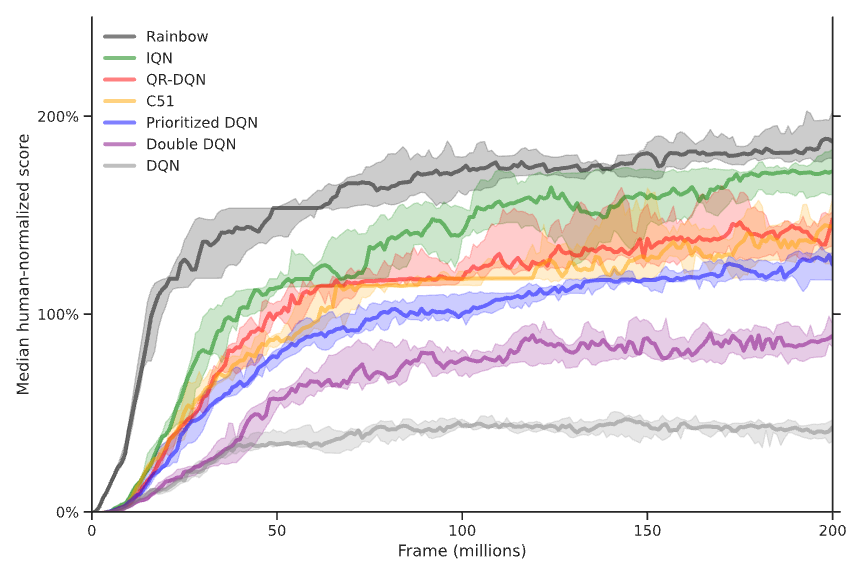
\includegraphics[height=1.5in]{figs/rainbow}
\caption{
  Plot of median human-normalized score over all 57 Atari games for
  various DQN agents.
  The yellow, red and green curves are distributional RL methods
  (\cref{sec:distributional}),
  namely categorical DQN (C51) (\cref{sec:C51})
  Quantile Regression DQN (\cref{sec:QRDQN}),
  and Implicit Quantile Networks \citep{IQN}.
  Figure from \url{https://github.com/google-deepmind/dqn_zoo}.
}
\label{fig:rainbow}
\end{figure}



Recently the ``Beyond the Rainbow'' paper \citep{beyond} proposed
several more extensions: 
\begin{itemize}
\item Use a larger CNN with residual connections,
  namely the Impala
  network from \citep{Espeholt2018}
  with the modifications (including the use of spectral normalization)
  proposed in
  \citep{Schmidt2021atari}.

  \item  Replace C51 with Implicit Quantile Networks \citep{IQN}.

  \item Use \keywordDef{Munchausen RL} \citep{Vieillard2020},
    which modifies
    the Q learning update rule by adding an entropy-like
    penalty.

  \item Collect 1 environment step from 64 parallel workers
    for each minibatch update (rather than taking many steps
    from a smaller number of workers).
\end{itemize}


\eat{
    \footnote{
    %
    The idea is as follows.
    First note that Q learning defines a greedy policy
    $\pi(a|s)=1$ iff $a = \argmax_{a'} Q(s,a')$,
    which we can convert to a stochastic policy
    $\pi(a|s) = \frac{\exp Q(s,a)}{\sum_{a'} Q(s,a')}$.
    Now consider the experience tuple
    $(s,a,r,s')$, so the Q learning
    target becomes $\targetV(s,a) = r + \max_{a'} Q^*(s',a')$.
Since $Q^*$ is unknown, we replace it with the current estimate
$Q_{\vw}(s',a')$ to get $\targetV(s,a) = r+q$ where $q=\max_{a'} Q_{\vw}(s',a')$.
However, this bootstrapping process can be unstable.
To help improve it, we can replace the target $r +q$ with
$r + \alpha \log \pi(a|s) + q$;
the motivation for this regularizer is that
the optimal policy should satisfy $\log \pi^*(a|s)$.
}
}


\subsubsection{Bigger, Better, Faster}
\label{sec:BBF}



At the time of writing this document (2024),
the SOTA on the 100k sample-efficient
Atari benchmark
\citep{Atari100k}
is obtained by the \keywordDef{BBF} algorithm of \citep{BBF}.
(BBF stands for ``Bigger, Better, Faster''.)
%This is arguably simpler than Rainbow.
It uses the following tricks,
in order of decreasing importance:
\begin{itemize}



\item Use a larger CNN with residual connections,
  namely a modified version of the Impala
  network from \citep{Espeholt2018}.

  \item Increase the \keywordDef{update-to-data} (UTD)
  ratio
  (number of times we update the Q function
  for every observation that is observed), in order to increase
  sample efficiency
  \citep{VanHasselt2019}.


\item Use a periodic soft reset of (some of) the network weights
to avoid loss of elasticity due to increased network updates, following the
\keywordDef{SR-SPR} method of \citep{DOro2022}.


\item Use n-step returns, as in \cref{sec:nsteps},
  and then gradually decrease (anneal) the n-step return from
 $n=10$ to $n=3$,
to reduce the bias over time.


\item Add weight decay.

\item Add a \keyword{self-predictive representation} loss
  (\cref{sec:self-predictive})
 to increase sample efficiency.

\item  Gradually increase the discount factor from
  $\gamma=0.97$ to $\gamma=0.997$,
  to encourage longer term planning once the model starts to be trained.\footnote{
  %
    The \keywordDef{Agent 57} method of  \citep{Badia2020}
  automatically learns the exploration rate and discount factor
  using a multi-armed bandit stratey,
  which lets it  be more exploratory or more exploitative,
  depending on the game. This resulted in super human performance
  on all 57 Atari games in ALE.
  However, it required 80 billion frames (environment steps)!
  This was subsequently reduced to the ``standard''
  200M frames in the \keywordDef{MEME} method of \citep{Kapturowski2022}.
  }


\item Drop noisy nets (which requires multiple network copies and thus slows
  down training due to increased memory use), since it does not help.

\item Use
  \keyword{dueling DQN} (see \cref{sec:duelingDQN}).

\item Use
  \keyword{distributional DQN}
  (see \cref{sec:distributional}).
  
%\item Use RNN models for the Q network,
%  as proposed in  the \keywordDef{R2D2} paper \citep{R2D2},
%  and used in many other papers.

\end{itemize}

\subsubsection{Other methods}

Many other methods have been proposed to reduce the sample complexity
of value-based RL while maintaining performance,
see e.g., the \keywordDef{MEME} paper of
\citep{Kapturowski2022}.






\chapter{Policy-based RL}
\label{sec:policySearch}



%https://lilianweng.github.io/lil-losg/2018/04/08/policy-gradient-algorithms.html

In the previous section, we considered methods that
estimate the action-value function, $Q(s,a)$,
from which we derive a policy.
%If $Q$ is close to $\Qopt$,
%the resulting policy will be near optimal.
%e.g., $\policy(a|s)=\ind{a=\argmax_a Q(s,a)}$
%or $\policy(a|s) = e^{Q(s,a)}/\sum_{a'} e^{Q(s,a')}$.
However, these methods have several disadvantages:
(1)  they can be difficult to apply to continuous action spaces;
(2) they may diverge if function approximation is used (see
\cref{sec:deadlyTriad});  
(3) the training of $Q$, often based on TD-style updates,
is not directly related to the expected return
garnered by the learned policy;
(4) they learn deterministic policies,
whereas in stochastic and partially observed environments,
stochastic policies are provably better
\citep{Jaakkola94}.

In this section, we discuss
\keywordDef{policy search} methods,
which directly optimize the parameters of the policy
so as to maximize its expected return.
We mostly focus on \keywordDef{policy gradient} methods,
that use the gradient of the loss to guide the search.
As we will see,  these policy methods often 
benefit from estimating a value or advantage function
to reduce the variance in the policy search process,
so we will also use techniques from \cref{sec:valueRL}.
The parametric policy will be denoted by 
$\pi_{\vtheta}(a|s)$.
For discrete actions, this can be a DNN with a softmax output.
For continuous actions, we can use a Gaussian output layer,
or a diffusion policy \citep{Ren2024}.

For more details on policy gradient methods, see \citep{weng2018PG,Lehmann2024}.



\eat{
\footnote{
%
To handle multimodal distributions, it has recently
become popular to use more expressive policy classes such as diffusion
models;
this is known as a \keywordDef{diffusion policy}
\citep{diffusionPolicy}.
However, since it is difficult to compute the probability
value of the output from diffusion, such models are usually
trained using behavior cloning (\cref{sec:BC}),
rather than the policy gradient methods we discuss in this section.
%(For a recent survey of other ways to apply diffusion in RL,
%see \citep{diffusionRL}.)
}
}

\section{The policy gradient theorem}
\label{sec:policyGradient}
\label{sec:PG}


%http://timvieira.github.io/blog/post/2019/04/20/the-likelihood-ratio-gradient/

We start by defining the objective function
for policy learning,
and then derive its gradient.
%We consider the episodic case.
%A similar result can be derived for the continuing case with the average reward
%criterion~\citep[Sec 13.6]{Suttonv2}.
The objective, which we aim to maximize, is defined as
\begin{align}
  J(\pi)  &\defeq \expectQ{\sum_{t=0}^{\infty} \gamma^t R_{t+1}}{\pi} \\
  &= \sum_{t=0}^{\infty} \gamma^t \sum_s \left(\sum_{s_0}
  p_0(s_0) p^{\pi}(s_0 \rightarrow s, t) \right)
  \sum_a \pi(a|s) R(s,a) \\
  &= \sum_s 
  \left(
  \sum_{s_0} \sum_{t=0}^{\infty} \gamma^t 
  p_0(s_0) p^{\pi}(s_0 \rightarrow s, t) \right)
  \sum_a \pi(a|s) R(s,a) \\
  &= \sum_s \rho^{\pi}(s)    \sum_a \pi(a|s) R(s,a) 
\end{align}
where we have defined the discounted state visitation
measure
\be
\statmeasure_{\pi}^{\gamma}(s) \defeq
\sum_{t=0}^{\infty} \gamma^t
\underbrace{\sum_{s_0}   p_0(s_0) p^{\pi}(s_0 \rightarrow s, t)}_{p_t^{\pi}(s)}
\ee
where
$p^{\pi}(s_0 \ra s, t)$ is the probability of going
from $s_0$ to $s$ in $t$ steps,
and
$p_t^{\pi}(s)$ is the marginal probability of being in state $s$
at time $t$ (after each episodic reset).
Note that $\statmeasure_{\pi}^{\gamma}$ is a measure of time spent in  non-terminal states,
but it is not a probability measure, since it is not normalized,
i.e., $\sum_s \statmeasure_{\pi}^{\gamma}(s) \neq 1$.
However, we may abuse notation and still treat it like a probability,
so we can write things like
\be
\expectQ{f(s)}{\statmeasure_{\pi}^{\gamma}(s)} =
\sum_s \statmeasure_{\pi}^{\gamma}(s) f(s)
\ee
Using this notation, we can define the objective as
\be
J(\pi) = \expectQ{R(s,a)}{\statmeasure_{\pi}^{\gamma}(s), \pi(a|s)}
\label{eqn:JJpi}
\ee
We can also define a normalized version of the measure $\statmeasure$
by noting that
$\sum_{t=0}^{\infty} \gamma^t = \frac{1}{1-\gamma}$ for $\gamma<1$.
Hence the normalized discounted state visitation distribution
is given by
\be
\statdistpol(s) = (1-\gamma) \statmeasure_{\pi}^{\gamma}(s)
= (1-\gamma) \sum_{t=0}^{\infty} \gamma^t p_t(s)
\label{eqn:statdistpol}
\ee
(Note the change from $\rho$ to $p$.)

Note that in 
\citep[Sec 13.2]{Suttonv2}, they use slightly different notation.
In particular, they assume $\gamma=1$,
and define the non-discounted state visitation measure
as $\eta(s)$ and the corresponding normalized version by $\mu(s)$.
This is equivalent to ignoring  the discount factor $\gamma^t$
when defining $\statmeasure_{\pi}(s)$.
This is standard practice in many implementations,
since we can just average over (unweighted)
trajectories when estimating
the objective and its gradient,
even though it
results in a biased estimate
\citep{Nota2020,Che2023}.

It can be shown that the gradient of the above objective is
given by
\begin{align}
\nabla_{\vtheta} J(\vtheta)
&=\sum_s \statmeasure_{\pi}^{\gamma}(s)
\sum_a Q^{\pi}(s,a) \nabla_{\vtheta} \pi_{\vtheta}(a|s)
\label{eqn:PGthm}
\\
&=\sum_s \statmeasure_{\pi}^{\gamma}(s)
\sum_a Q^{\pi_{\vtheta}}(s,a) \pi_{\vtheta}(a|s) \nabla_{\vtheta} \log \pi_{\vtheta}(a|s) \\
&=\expectQ
{Q^{\pi_{\vtheta}}(s,a) \nabla_{\vtheta} \log \pi_{\vtheta}(a|s)}
    {\statmeasure_{\pi}^{\gamma}(s) \pi_{\vtheta}(a|s)} 
\label{eqn:SFE}
\end{align}
This is known as the \keywordDef{policy gradient theorem}
\citep{Sutton99b}.
In statistics, the term $\nabla_{\vtheta} \log \pi_{\vtheta}(\va|\vs)$
is called the (Fisher) \keywordDef{score function}\footnote{
%
This is distinct from the Stein score,
which is the gradient wrt the argument of the log probability,
$\nabla_{\va} \log \pi_{\vtheta}(\va|\vs)$,
as used in diffusion.
},
so sometimes \cref{eqn:SFE}
is called the \keywordDef{score function estimator}
or \keywordDef{SFE} \citep{Fu2015,Mohamed2020}.



\section{REINFORCE}
\label{sec:REINFORCE}
\label{sec:reinforceOpt}
\label{sec:reinforce}

% Pieter Abeel lecture notes
%https://drive.google.com/file/d/0BxXI_RttTZAhY216RTMtanBpUnc/view


% Sutton p327
One way to apply the policy gradient theorem
to optimize a policy is to use stochastic gradient ascent.
Theoretical results concerning the convergence
and sample complexity of such
methods can be found in \citep{Agarwal2021}.

To implement such a method,
let
$\traj=(s_0,a_0,r_0,s_1,\ldots,s_T)$ be
a trajectory created by sampling from $s_0\sim\initdist$
and then following $\polapprox$.
Then we have
\begin{align}
\nabla_{\vtheta} \polval(\polapprox)
&=
\sum_{t=0}^{\infty} \gamma^t \expectQ{
  \nabla_{\vtheta} \log \polapprox(a_t|s_t) \Qpolapprox(s_t,a_t)}
    {p_t(s) \polapprox(a_t|s_t)} \\
  &\approx \sum_{t=0}^{T-1} \gamma^t \return_t \nabla_{\vtheta} \log\polapprox(a_t|s_t)
\end{align}
where the return  is defined as follows
\begin{align}
\return_t &\defeq r_t + \gamma r_{t+1} + \gamma^2 r_{t+2} + \cdots
+ \gamma^{T-t-1} r_{T-1} 
= \sum_{k=0}^{T-t-1} \gamma^k r_{t+k}
= \sum_{j=t}^{T-1} \gamma^{j-t} r_j
\end{align}
See \cref{algo:REINFORCE} for the pseudocode.

\begin{algorithm}
\dontprintsemicolon
\caption{REINFORCE (episodic version)}
\label{algo:REINFORCE}
Initialize policy parameters $\vtheta$\\
\Repeat{converged}
       {
         Sample an episode $\traj=(s_0, a_0, r_0, s_1, \ldots, s_T)$ using $\polapprox$ \\
         %Compute $\return_t$ for all $t\in\{0,1,\ldots,T-1\}$ using \cref{eqn:rl-return} \\
         \For{$t=0,1,\ldots,T-1$}{
           $\return_t = \sum_{k=t+1}^T \gamma^{k-t-1} R_k$ \\
           $\vtheta \assign \vtheta + \lr_{\vtheta} \gamma^t \return_t
           \nabla_{\vtheta} \log \policy_{\vtheta}(a_t|s_t)$
         }
}
\end{algorithm}

In practice, estimating the policy gradient using
\cref{eqn:SFE} can have a high variance.
A \keywordDef{baseline} function $b(s)$ can be used for variance reduction
to get
\begin{align}
\nabla_{\vtheta} \polval(\polapprox) = 
 \expectQ{\nabla_{\vtheta} \log \polapprox(a|s) (\Qpolapprox(s,a) - b(s))}
{\statmeasure_{\vtheta}(s) \polapprox(a|s)}
\label{eqn:PGthmBaseline}
\end{align}
Any function that satisfies $\expect{\nabla_{\vtheta} b(s)}=0$ is a valid
baseline.
This follows since
\be
\sum_a  \nabla_{\vtheta} \pi_{\vtheta}(a|s) (Q(s,a)-b(s))
= \nabla_{\vtheta} \sum_a \pi_{\vtheta}(a|s) Q(s,a)
-\nabla_{\vtheta} [\sum_a \pi_{\vtheta}(a|s)] b(s)
= \nabla_{\vtheta} \sum_a \pi_{\vtheta}(a|s) Q(s,a) - 0
\ee
A common choice for the baseline is $b(s) = \Vpolapprox(s)$.
This is a good choice since $\Vpolapprox(s)$ and $Q(s,a)$ are correlated
and have similar magnitudes,
so the scaling factor in front of the gradient term will be small.
%(See also \citep{Wu2018} for an action-dependent baseline.)

Using this we get an update of the following form
\begin{align}
  \vtheta \assign \vtheta + \lr \sum_{t=0}^{T-1}
  \gamma^t (G_t - b(s_t)) \nabla_{\vtheta} \log\polapprox(a_t|s_t)
\label{eqn:REINFORCE}
\end{align}
This is 
is called the \keywordDef{REINFORCE} estimator
\citep{Williams1992}.\footnote{
  %
  The term 
``REINFORCE'' is an acronym for
``REward Increment = nonnegative Factor x Offset
Reinforcement x Characteristic Eligibility''.
The phrase ``characteristic eligibility'' refers to  the
$\nabla \log \polapprox(a_t|s_t)$ term;
the phrase ``offset reinforcement'' refers to the
$\return_t-b(s_t)$ term;
and the phrase ``nonnegative factor''
refers to the learning rate $\lr$ of SGD.
} %
The update equation
 can be interpreted as follows:
we compute the sum of discounted future rewards
induced by a trajectory, compared to a
baseline,  and if this is positive, we increase
$\vtheta$ so as to make this trajectory more likely,
otherwise we decrease $\vtheta$.
Thus, we reinforce good behaviors,
and reduce the chances of generating bad ones.



\eat{
\cref{algo:REINFORCEbaseline} gives the pseudocode
where we use  separate learning rates
for the two objectives.

\begin{algorithm}
\dontprintsemicolon
\caption{REINFORCE (episodic) with value function baseline}
\label{algo:REINFORCEbaseline}
Initialize policy parameters $\vtheta$, baseline parameters $\vw$\\
\Repeat{converged}
       {
         Sample an episode $\traj=(s_0, a_0, r_0, s_1, \ldots, s_T)$ using $\polapprox$ \\
         %Compute $\return_t$ for all $t\in\{0,1,\ldots,T-1\}$ using \cref{eqn:rl-return} \\
         \For{$t=0,1,\ldots,T-1$}{
           $\return_t = \sum_{k=t+1}^T \gamma^{k-t-1} R_k$ \\
           $\delta_t = \return_t - \Vapprox(s_t)$  \\
           $\vw \assign \vw - \lr_{\vw} \delta_t \nabla_{\vw}
           \Vapprox(s_t)$  \\
           $\vtheta \assign \vtheta + \lr_{\vtheta} \gamma^t \delta_t
           \nabla_{\vtheta} \log \policy_{\vtheta}(a_t|s_t)$ 
         }
}
\end{algorithm}
}


\section{Actor-critic methods}
\label{sec:actorCritic}
\label{sec:AC}



An \keywordDef{actor-critic} method \citep{Barto1983}
uses the policy gradient method,
but where the expected return $G_t$ is estimated
using temporal difference learning
of a value function instead of MC rollouts.
(The term ``actor'' refers to the policy,
and the term ``critic'' refers to the value function.)
The use of bootstrapping in TD updates
allows more efficient learning of the value function
compared to MC, and further reduces the variance.
In addition, it allows us to develop a fully online, incremental
algorithm, that does not need to wait until the end of the trajectory
before updating the parameters.


\subsection{Advantage actor critic (A2C)}
\label{sec:A2C}
\label{sec:A3C}

% Sutton p331
Concretely, consider the use of the one-step TD method
to estimate the return in the episodic case,
i.e., we replace $\return_t$ with
$\return_{t:t+1}=r_t+ \gamma \Vapprox(s_{t+1})$.
If we use $\Vapprox(s_t)$ as a baseline,
the REINFORCE update in \cref{eqn:REINFORCE} becomes
\begin{align}
\vtheta 
&\assign \vtheta + \lr \sum_{t=0}^{T-1} \gamma^t \left(G_{t:t+1} - \Vapprox(s_t)\right) \nabla_{\vtheta} \log\polapprox(a_t|s_t) \\
&= \vtheta + \lr \sum_{t=0}^{T-1} \gamma^t \big(r_t+ \gamma \Vapprox(s_{t+1}) - \Vapprox(s_t)\big) \nabla_{\vtheta} \log\polapprox(a_t|s_t)
\end{align}

%This  can be extended to the off-policy
%setting as explained in e.g., \citep{Degris2012,Zhang2019}.
%https://medium.com/@jonathan_hui/rl-policy-gradients-explained-advanced-topic-20c2b81a9a8b



Note that
$\delta_t = r_{t+1} + \gamma \Vapprox(s_{t+1}) -\Vapprox(s_t)$
is a single sample approximation
to the advantage function $A(s_t,a_t) = Q(s_t,a_t) - V(s_t)$.
%We can alternatively learn the advantage function
%directly, and use $A(s_t,a_t)$ instead
%of $\return_{t:T}$ (as in vanilla REINFORCE),
%or $\return_t^{(1)}$ (as in REINFORCE with a TD(0) baseline).
This method is therefore called 
\keywordDef{advantage actor critic} or \keywordDef{A2C}.
See \cref{algo:A2C} for the pseudo-code.\footnote{
%
In \citep{A3C}, they proposed
a distributed version of A2C known as
\keywordDef{A3C} 
which stands for  ``asynchrononous advantage actor critic''. 
}
(Note that $V_{\vw}(s_{t+1})=0$ if $s_t$ is a done state,
representing the end of an episode.)
Note that this is an on-policy algorithm,
where we update the value function $V_{\vw}^{\pi}$
to reflect the value of the current policy $\pi$.
See \cref{sec:bilevel} for further discussion of this point.

% https://github.com/DLR-RM/stable-baselines3/blob/master/stable_baselines3/a2c/a2c.py


\begin{algorithm}
\dontprintsemicolon
\caption{Advantage actor critic (A2C) algorithm (episodic)}
\label{algo:A2C}
Initialize actor parameters $\vtheta$, critic parameters $\vw$\\
\Repeat{converged}
       {
       Sample starting state $s_0$ of a new episode \\
       \For{$t=0,1,2,\ldots$}
       {
         Sample action $a_t \sim \polapprox(\cdot|s_t)$ \\
         $(s_{t+1},r_t,\done_t) = \text{env.step}(s_t,a_t)$ \\
        $\targetV_t = r_t + \gamma (1-\done_t) \Vapprox(s_{t+1})$       // Target \\
       $\delta_t = \targetV_t - \Vapprox(s_t)$ // Advantage \\
           $\vw \assign \vw  + \lr_{\vw} \delta_t \nabla_{\vw}
       \Vapprox(s_t)$ // Critic \\
           $\vtheta \assign \vtheta + \lr_{\vtheta} \gamma^t \delta_t
       \nabla_{\vtheta} \log \polapprox(a_t|s_t)$ // Actor \\
       \If{$\done_t=1$}{break}
         }
}
\end{algorithm}

In practice, we should use a stop-gradient
operator on the target value for the TD update,
for reasons  explained in \cref{sec:deadlyTriad}.
Furthermore, it is common to add an entropy term
to the policy, to act as a regularizer
(to ensure the policy remains stochastic, which smoothens
the loss function --- see \cref{sec:SAC}).
If we use a shared network with separate value  and policy heads,
we need to use a single loss function for training all the parameters
$\vphi$.
Thus we get the following loss, for each trajectory,
where we want to minimize TD loss,
maximize the policy gradient (expected reward) term,
and maximize the entropy term.
\begin{align}
  \loss(\vphi;\tau) &= \frac{1}{T} \sum_{t=1}^T \left[
    \lambda_{TD} \loss_{TD}(s_t,a_t,r_t,s_{t+1})
    -    \lambda_{PG} J_{PG}(s_t,a_t,r_t,s_{t+1})
    -    \lambda_{ent} J_{ent}(s_t)
    \right]
  \label{eqn:ACloss}\\
  \targetV_t &= r_t + \gamma (1-\done(s_t)) V_{\vphi}(s_{t+1}) \\
  \loss_{TD}(s_t,a_t,r_t,s_{t+1})  &= (\stopgrad(\targetV_t) - V_{\phi}(s))^2 \\
  J_{PG}(s_t,a_t,r_t,s_{t+1}) &= (\stopgrad(\targetV_t - V_{\phi}(s_t))
  \log \pi_{\vphi}(a_t|s_t) \\
  J_{ent}(s_t) &= -\sum_a \pi_{\vphi}(a|s_t) \log \pi_{\vphi}(a|s_t)
\end{align}
To handle the dynamically varying scales of the different loss functions,
we can use 
the \keywordDef{PopArt} method
of \citep{van-Hasselt2016,Hessel2019}
to allow for a fixed set of hyper-parameter values for $\lambda_i$.
(PopArt  stands for
``Preserving Outputs Precisely, while Adaptively Rescaling Targets''.)

\eat{
\begin{align}
  \loss(\vphi;\tau) = \frac{1}{T} \sum{t=1}^T \left[
    \lambda_{TD} (\stopgrad(\targetV_t) - V_{\vphi}(\vs_t))^2
    -    \lambda_{PG} (\stopgrad(\targetV_t - V_{\vphi}(\vs_t))
    -    \lambda_{ent} \entropy(\pi_{\vphi}(\cdot|\vs_t))
    \right]
  \end{align}
}

\eat{
We can then accumulate  the following gradients
over each sampled trajectory:
\begin{align}
  \nabla_{\vw}  &= -\frac{1}{2T} \sum_t
  \nabla_{\vw} (\targetV_t - V_{\vw}(s_t))^2 
  = \frac{1}{T} \sum_t  (\targetV_t - V_{\vw}(s_t)) \nabla_{\vw} V_{\vw}(s_t) \\
  \nabla_{\vtheta} &= \frac{1}{T} \sum_t
  (\targetV_t - V_{\vw}(s_t)) \nabla_{\vtheta} \log \pi_{\vtheta}(a_t|s_t)
  \end{align}
The second gradient ignores the discount term $\gamma^t$,
but omitting this is standard practice,
even though it
results in a biased estimate
\citep{Nota2020,Che2023}.
}


\eat{
For a more practical minibatch version,
based on \citep{Ivanov2019},
see \cref{algo:A2C}.
}

\subsection{Generalized advantage estimation (GAE)}
\label{sec:GAE}

%\subsection{AC with $n$-step critics}

In A2C, we replaced the high variance, but unbiased,
MC return $G_t$
with the low variance, but biased,
one-step bootstrap return $G_{t:t+1} = r_t + \gamma V_{\vw}(s_{t+1})$.
More generally, we can compute the
$n$-step estimate
\begin{align}
G_{t:t+n} =
r_t + \gamma r_{t+1} + \gamma^2 r_{t+2}
+ \cdots + \gamma^{n-1} r_{t+n-1} + \gamma^n \Vapprox(s_{t+n})
\end{align}
and thus obtain  the (truncated) $n$-step advantage estimate as follows:
\be
A_{\vw}^{(n)}(s_t,a_t) = G_{t:t+n} - \Vapprox(s_t)
\ee
Unrolling to infinity, we get
% https://nn.labml.ai/rl/ppo/gae.html
\begin{align}
  A_t^{(1)} &= r_t + \gamma v_{t+1} - v_t  \\
  A_t^{(2)} &= r_t + \gamma r_{t+1} + \gamma^2 v_{t+2} - v_t  \\
  &\vdots \\
  A_t^{(\infty)} &= r_t + \gamma r_{t+1} + \gamma^2 r_{t+2} +\cdots - v_t 
  \end{align}
$A_t^{(1)}$ is high bias but low variance,
and $A_t^{(\infty)}$  is unbiased but high variance.


%https://nn.labml.ai/rl/ppo/gae.html
% https://github.com/google-deepmind/rlax/blob/master/rlax/_src/multistep.py#L39
% https://github.com/EdanToledo/Stoix/blob/main/stoix/utils/multistep.py#L12
% https://github.com/luchris429/purejaxrl/blob/main/purejaxrl/ppo.py#L142
%https://github.com/DLR-RM/stable-baselines3/blob/master/stable_baselines3/common/buffers.py#L402

Instead of using a single value of $n$, we can take
a weighted average.
That is, we define
\be
A_t = \frac{\sum_{n=1}^T w_n A_t^{(n)}}{\sum_{n=1}^T w_n}
\ee
If we set $w_n = \lambda^{n-1}$ we get the following simple recursive
calculation:
\begin{align}
  \delta_t &= r_t + \gamma v_{t+1} - v_t \\
  A_t &= \delta_t + \gamma \lambda \delta_{t+1} + \cdots +
  (\gamma \lambda)^{T-t+1} \delta_{T-1} = \delta_t + \gamma \lambda
  A_{t+1}
  \end{align}
Here $\lambda \in [0,1]$ is a parameter that controls the bias-variance
tradeoff: larger values decrease the bias but increase the variance.
This is called \keywordDef{generalized advantage estimation}
(\keywordDef{GAE})~\citep{GAE}.
See \cref{algo:GAE} for some pseudocode.
Using this, we can define a general actor-critic
method, as shown in \cref{algo:AC}.

\begin{algorithm}
\dontprintsemicolon
\caption{Generalized Advantage Estimation}
\label{algo:GAE}
$\text{def GAE}(r_{1:T},v_{1:T}, \gamma, \lambda)$\\
$A'=0$ \\
\For{$t=T:1$}{
  $\delta_t = r_t + \gamma v_{t+1} - v_t$ \\
  $A' = \delta_t + \gamma \lambda A'$ \\
  $A_t = A'$ // advantage \\
  $\targetV_t = A_t + v_t$ // TD target 
}
Return $(A_{1:T}), \targetV_{1:T})$
%       Return $(\stopgrad(A_{1:T}), \stopgrad(\targetV_{1:T}))$
\end{algorithm}


\begin{algorithm}
\dontprintsemicolon
\caption{Actor critic with GAE}
\label{algo:AC}
Initialize  parameters $\vphi$,
environment state $s$\\
\Repeat{converged}
{
  $(s_1,a_1,r_1,\ldots,s_T)= \text{rollout}(s, \pi_{\vphi})$ \\
  $v_{1:T} = V_{\vphi}(s_{1:T})$ \\
  $(A_{1:T}, \targetV_{1:T}) = \stopgrad(\text{GAE}(r_{1:T}, v_{1:T}, \gamma, \lambda))$
  \\
  $\loss(\vphi) = \frac{1}{T}\sum_{t=1}^T \left[
    \lambda_{TD} (V_{\vphi}(s_t) - \targetV_t)^2
    -\lambda_{PG} A_t \log \pi_{\vphi}(a_t|s_t)
    -\lambda_{ent} \entropy(\pi_{\vphi}(\cdot|s_t)) \right]$ \\
  $\vphi := \vphi - \lr \nabla \loss(\vphi)$
  }
\end{algorithm}



\eat{
We can implement this as shown in \cref{algo:ACn},
following \citep[Algo 4.4]{Plaat2022}.
%(In practice, the nested sum over $\sum_t$ and $\sum_k$
%would be computed by a single backwards sum from $t=T-1$ downto 0.)

\begin{algorithm}
\dontprintsemicolon
\caption{A2C with $n$-step bootstrapping}
\label{algo:ACn}
Initialize actor parameters $\vtheta$, critic parameters $\vw$,
environment state $s$\\
\Repeat{converged}
{
         $(\tau,s) = \text{rollout}(s, \pi_{\vtheta})$ \\
         $(\vtheta, \vw) = \text{AC-step}(\vtheta, \vw, \tau)$ \\
}
.\\
$\text{def AC-step}(\vtheta,\vw,\tau)$: \\
Let $(s_0,a_0,r_0,\ldots,s_T)=\tau$ \\
\For{$t=0:T-1$}{
  $G_t = \left[\sum_{k=0}^{n-1} \gamma^k r_{t+k}  \right]
  + \gamma^n V_{\vw}(s_{t+n})$ \\
  $A_t = G_t - V_{\vw}(s_t)$
}
$\loss_{\vw} = \sum_t A_t^2$ \\
$J_{\vtheta} = \sum_t A_t \log \pi_{\vtheta}(a_t|s_t)$ \\
$\vw \assign \vw - \lr_{\vw} \nabla \loss_{\vw}$\\
$\vtheta \assign \vtheta + \lr_{\vtheta} \nabla J_{\vtheta}$ \\
       Return $(\vtheta,\vw)$
\end{algorithm}
}



\eat{
with weight proportional to $\lambda^n$
for $A_{\vw}^{(n)}(s_t,a_t)$, as in TD($\lambda$).
The average can be shown to be equivalent to
\begin{align}
A_{\vw}^{(\lambda)}(s_{t}, a_{t}) \defeq \sum_{\ell=0}^{\infty}
 (\gamma \lambda)^{\ell} \delta_{t+l}
 \label{eqn:ApolSum}
\end{align}
where $\delta_t= r_t + \gamma \Vapprox(s_{t+1}) - \Vapprox(s_t)$
is the TD error at time $t$.


In the episodic case, we can implement GAE
by modifying the $n$-step bootstrap AC algorithm
in \cref{algo:ACn}:
we just replace $Q_t$
by the $\lambda$-return $\Lambda_t$, which is computed by iterating backwards
from the end of the trajectory to the start:
\begin{align}
  \Lambda_t  = \begin{cases}
    r_t + \gamma (1-d_t)
    \left[ (1-\lambda) V(s_{t+1}) + \lambda \Lambda_{t+1} \right]
    &\mbox{if $t<T$}  \\
    V(s_T) &\mbox{otherwise}
    \end{cases}
  \end{align}
We can also develop a fully online version
using eligibility traces
(see \citep[Ch.12]{Suttonv2} for  details).
}


We can generalize this approach even further,
by using gradient estimators of the form
\be
\nabla J(\vtheta) = \expect{
\sum_{t=0}^{\infty} \Psi_t \nabla \log \policy_{\vtheta}(a_t|s_t)}
\ee
where $\Psi_t$ may be any of the following:
\begin{align}
  \Psi_t &=  \sum_{i=t}^{\infty} \gamma^i r_i
  & \text{Monte Carlo target}\\
%  \Psi_t &= Q_{n}(s_t,a_t) = \sum_{i=t}^{n-1} \gamma^i r_i
%  + \gamma^n V_{\vw}(s_n) & \text{Bootstrap $n$-step target}\\
  \Psi_t &=  \sum_{i=t}^{\infty} \gamma^i r_i
  -V_{\vw}(s_t) & \text{MC with baseline}\\
%  \Psi_t &= A_{\text{MC}}(s_t,a_t) = \sum_{i=t}^{n-1} \gamma^i r_i
%  + \gamma^n V_{\vw}(s_n) -V_{\vw}(s_t) & \text{Baseline +
  %  bootstrap}\\
  \Psi_t &= A_{\vw}(s_t,a_t) & \text{advantage function} \\
  \Psi_t &= Q_{\vw}(s_t,a_t) & \text{Q function} \\
  \Psi_t &= r_t + V_{\vw}(s_{t+1}) - V_{\vw}(s_t) & \text{TD residual}
  \end{align}

\eat{
  \begin{align}
\Psi_t &= \sum_{t=0}^{\infty} r_t \; \text{: total reward of trajectory}\\
\Psi_t &= \sum_{t'=t}^{\infty} r_{t'} \; \text{: reward following $a_t$} \\
\Psi_t &= \sum_{t'=t}^{\infty} r_{t'} - b(s_t) \; \text{: baselined
version of previous formula} \\
\Psi_t &= \Qpol(s_t,a_t) \; \text{: action-value function} \\
\Psi_t &= \Apol(s_t,a_t) \; \text{: advantage function} \\
\Psi_t &= r_t + \Vpol(s_{t+1}) - \Vpol(s_t) \; \text{: TD residual}
  \end{align}
  }
See \citep{GAE} for details.





\subsection{Two-time scale actor critic algorithms}
\label{sec:twoTimeScale}
\label{sec:bilevel}

In standard AC, we update the actor and critic in parallel.
However, it is better
to let critic $V_{\vw}$ learn
using a faster learning rate (or more updates),
so that it reflects the value of the current policy $\pi_{\vtheta}$
more accurately, in order to get better gradient estimates
for the policy update.
This is 
known as \keyword{two timescale learning}
or \keywordDef{bilevel optimization}
\citep{Yu2017TD,Zhang2019timescale,Hong2023,Zheng2022AC,Lorraine2024}.
(See also \cref{sec:MBRLgame}, where we discuss RL
from a game theoretic perspective.)

%% \footnote{
%% %
%% In \citep{Hanna2024}, they found that discretizing
%% the action space and replacing squared error with
%% cross-entropy error gave better results.
%% This is
%% consistent with other papers
%% \citep{Imani2018,Farebrother2024}
%% which  show that classification loss can be better even
%% for regression problems.
%% }

\eat{
\subsection{Advantage-weighted regression}
\label{sec:AWR}



Recall from A2C (\cref{sec:A2C})
that the policy update takes the form
$\vtheta \assign \vtheta + \lr_{\vtheta} \gamma^t \delta \nabla_{\vtheta} \log \pi_{\vtheta}(a|s)$,
where $\delta = r + \gamma \Vapprox(s') - \Vapprox(s)$
is the TD error,
and we sample $(s,a,s',r)$ from the environment and current policy.
Note that $\delta$
is an approximation to the advantage function at the current state $s$.
If we treat the advantage function as frozen,
we can compute an
approximation to the gradient of the expected reward
using 
$\nabla_{\vtheta} J(\pi_{\vtheta})
\approx \expect{A_{\vw,\vtheta}(\vs,\va) \nabla_{\vtheta} \log \pi_{\vtheta}(\va|\vs)}$,
where the expectation is wrt states drawn
from the state distribution, $\vs \sim d_{\pi_{\vtheta}}$,
and actions drawn from the current policy,
$\va \sim \pi_{\vtheta}(\cdot|\vs)$.
We can compute an empirical $N$-sample
approximation to the corresponding
implicit loss by defining


From \cref{algo:A2C}, we see that
the policy loss for a sampled trajectory
has the form
\be
J(\vtheta) = \frac{1}{T} \sum_{t=1}^T
A_{\vw}(\vs_t,\va_t) \log \pi_{\vtheta}(\va_t|\vs_t)
\ee
In the case of a Gaussian policy,
this becomes
\be
\loss(\vtheta) = \frac{1}{T} \sum_{t=1}^T
A_{\vw}(\vs_t,\va_t) \half ||\va_t-\pi_{\vtheta}(\vs_t)||_2^2
\ee
which is a weighted regression loss.
The value function loss has the form
\be
\loss(\vw) = \frac{1}{T}
\sum_{t=1}^T (r_t + \gamma V_{\vw}(\vs_{t+1}) -V_{\vw}(\vs_t))^2
\ee
We can therefore alternate between optimizing the value function,
which is a nonlinear least squares problem,
and optimizing the policy,
which is a weighted  maximum likelihood problem.
This approach is known as 
\keywordDef{reward-weighted regression} 
\citep{Peters2007}
or \keywordDef{advantage-weighted regression} or \keywordDef{AWR}
\citep{Peng2019awr,Kozakowski2022}.

In the above approach,
we can think of the actor and critic as each computing a
``best response'' to the other player at each step.
This game-theoretic perspective is discussed in more detail
in \cref{sec:MBRLgame}.
There we mention that the best response strategy
can lead to unstable algorithms.
A better approach is the two time scale methods
 discussed in \cref{sec:twoTimeScale}.

 }


\subsection{Natural policy gradient methods}
\label{sec:naturalAC}
\label{sec:naturalPG}
\label{sec:NPG}


In this section, we discuss an improvement to policy
gradient methods that uses preconditioning to speedup convergence.
In particular, we replace gradient descent with  
\keywordDef{natural gradient descent} (\keywordDef{NGD})
\citep{Amari1998,Martens2020},
which we explain below. We then show how to combine it with actor-critic.


\subsubsection{Natural gradient descent}

NGD is a second order method
for optimizing the parameters of
(conditional) probability distributions, such as policies,
$\pi_{\vtheta}(\va|\vs)$.
It typically converges faster and more robustly than
SGD, but is computationally more expensive.

Before we explain NGD, let us review standard
SGD, which is an update of the following form
\be
\vtheta_{k+1} = \vtheta_k - \lr_k \vg_k
\ee
where $\vg_k = \nabla_{\vtheta} \loss(\vtheta_k)$
is the gradient of the loss at the previous parameter values,
and $\lr_k$ is the learning rate.
It can be shown that the above update is equivalent
to minimizing a locally linear approximation to the loss,
$\hat{\loss}_k$,
subject to the constraint that
the new parameters do not move too far (in Euclidean distance)
from the previous parameters:
\begin{align}
\vtheta_{k+1} &= \argmin_{\vtheta}
\hat{\loss}_k(\vtheta) \myst ||\vtheta-\vtheta_k||_2^2 \leq \epsilon
\\
\hat{\loss}_k(\vtheta) &= \loss(\vtheta_k) + \vg_k^\trans(\vtheta-\vtheta_k)
\end{align}
where the step size $\lr_k$ is  proportional to $\epsilon$.
This is called a \keywordDef{proximal update}
\citep{proximal}.

One problem with the SGD update is that Euclidean distance
in parameter space does not make sense for probabilistic models.
For example, consider
comparing two Gaussians,
$p_{\vtheta} = p(y|\mu,\sigma)$
and
$p_{\vtheta'} = p(y|\mu',\sigma')$.
The (squared) Euclidean distance between the parameter vectors
decomposes as $||\vtheta - \vtheta'||_2^2 = (\mu-\mu')^2 + (\sigma-\sigma')^2$.
However, the predictive distribution has the form
$\exp(-\frac{1}{2\sigma^2} (y-\mu)^2)$,
so changes in $\mu$ need to be measured
relative to $\sigma$.
This is illustrated in 
\cref{fig:honkelaGaussians}(a-b),
which shows
two univariate Gaussian distributions (dotted and solid lines)
whose means differ  by $\epsilon$.
In \cref{fig:honkelaGaussians}(a), they share the same small variance
$\sigma^2$,
whereas in  \cref{fig:honkelaGaussians}(b), they share the same large variance.
It is clear that the difference in   $\mu$
matters much more (in terms of the effect on the distribution)
when the variance is small.
%(\cref{fig:honkelaGaussians}(c-d) shows a similar effect when
Thus we see that the two parameters interact with each other,
which the Euclidean distance cannot capture.

\begin{figure}
\centering
\begin{subfigure}[b]{0.45\textwidth}
\centering
\includegraphics[height=1.5in]{figs/meanchange_lowvar}
\caption{ }
\end{subfigure}
~
\begin{subfigure}[b]{0.45\textwidth}
\centering
\includegraphics[height=1.5in]{figs/meanchange_highvar}
\caption{ }
\end{subfigure}
\caption{
 Changing the mean of a Gaussian by a fixed amount (from solid to
 dotted curve)
can have more impact
when the (shared) variance is small (as in a)
compared to when the variance is large (as in b).
Hence the impact (in terms of prediction accuracy)
of a change to $\mu$
depends on where the optimizer is in
$(\mu,\sigma)$ space.
\figtaken{Figure 3 of \citep{Honkela2010}, reproduced from 
\citep{ValpolaPhD}.}
\figthanks{Antti Honkela}.
}
\label{fig:honkelaGaussians}
\end{figure}

The key to NGD is to measure the notion of distance
between two probability distributions
in terms of the KL divergence.
This can be approximated in terms of
the \keywordDef{Fisher information matrix}  (FIM).
In particular, for any given input $\xdata$,
we have
\be
  \KLpq{p_{\params}(\vy|\xdata)}{p_{\params+\vdelta}(\vy|\xdata)}
  \approx
\half \vdelta^\trans \vFisher_{\xdata} \vdelta
\ee
where $\vFisher_{\xdata}$ is the FIM
\be
\vFisher_{\xdata}(\params)
= -\expectQ{\nabla^2 \log p_{\params}(\vy|\xdata)}{p_{\params}(\vy|\xdata)}
= \expectQ{(\nabla \log p_{\params}(\vy|\xdata))
(\nabla \log p_{\params}(\vy|\xdata))^\trans}{p_{\params}(\vy|\xdata)}
\ee
We  now replace the Euclidean distance
between the parameters,
$d(\vtheta_k, \vtheta_{k+1}) = ||\vdelta||_2^2$,
with 
\be
d(\vtheta_k, \vtheta_{k+1})
= \vdelta^\trans \vFisher_k \vdelta_k
\ee
where $\vdelta = \vtheta_{k+1}-\vtheta_k$
and $\vFisher_k = \vFisher_{\vx}(\vtheta_k)$
for a randomly chosen input $\vx$.
This gives rise to the following constrained
optimization problem:
\be
\vdelta_k = \argmin_{\vdelta}
\hat{\loss}_k(\vtheta_k + \vdelta) \myst
\vdelta^\trans \vFisher_k \vdelta \leq \epsilon
\ee
If we replace the constraint with a Lagrange multiplier,
we get the unconstrained objective:
\be
J_k(\vdelta) = \loss(\vtheta_k) + \vg_k^\trans \vdelta
+ \lr_k \vdelta^\trans \vFisher_k \vdelta 
\ee
Solving $J_k(\vdelta)=0$ gives the update
\be
\vdelta =  -\lr_k \vFisher_k^{-1} \vg_k
\ee
The term $\vFisher^{-1} \vg$
is called the \keywordDef{natural gradient}.
This is equivalent to  a preconditioned gradient update,
where we use the inverse FIM as a preconditioning matrix.
We can compute  the (adaptive) learning rate using
\be
\eta_k = \sqrt{\frac{\epsilon}{\vg_k^\trans \vF_k^{-1} \vg_k}}
\ee


Computing the FIM can be hard.
A simple approximation is to replace
the model's distribution with the empirical distribution.
In particular, define
 $\pemp(\xdata,\vy) = \frac{1}{N} \sum_{n=1}^N \delta_{\xdata_n}(\xdata) \delta_{\vy_n}(\vy)$,
$\pemp(\xdata) = \frac{1}{N} \sum_{n=1}^N \delta_{\xdata_n}(\xdata)$
and
$p_{\vtheta}(\vx,\vy) =  \pemp(\vx) p(\vy|\vx,\vtheta)$.
Then we can compute the \keywordDef{empirical Fisher}
\citep{Martens2016Thesis}
as follows:
\begin{align}
\vFisher(\vtheta) &= \expectQ{
\nabla \log p(\vy|\xdata,\params)
\nabla \log p(\vy|\xdata,\params)^\trans}
{p_{\vtheta}(\vx,\vy)} \\
 &\approx
\expectQ{
\nabla \log p(\vy|\xdata,\params)
\nabla \log p(\vy|\xdata,\params)^\trans}
{\pemp(\vx,\vy)} \\
&=
\frac{1}{|\data|}
\sum_{(\xdata,\vy) \in \data}
\nabla \log p(\vy|\xdata,\params)
\nabla \log p(\vy|\xdata,\params)^\trans
\end{align}

\subsubsection{Natural actor critic}

To apply NGD to RL, we can adapt
the A2C algorithm in \cref{algo:AC}.
In particular, define
\be
\vg_{kt} = \nabla_{\vtheta_k} A_t \log \pi_{\vtheta}(\va_t|\vs_t)
\ee
where $A_t$ is the advantage function at step $t$
of the random trajectory generated by the policy
at iteration  $k$.
Now we compute
\be
\vg_k = \frac{1}{T} \sum_{t=1}^T \vg_{kt},
\;
\vF_k = \frac{1}{T} \sum_{t=1}^T \vg_{kt} \vg_{kt}^\trans
\label{eqn:NACfisher}
\ee
and compute
$\vdelta_{k+1} = -\lr_k \vF_k^{-1} \vg_k$.
This approach is called \keywordDef{natural policy gradient}
\citep{Kakade2001,Rajeswaran2017}.

We can compute $\vF_k^{-1} \vg_k$ without having
to invert $\vF_k$ by using the conjugate gradient method,
where each CG step uses efficient
methods for Hessian-vector products \citep{Pearlmutter1994}.
This is called
\keywordDef{Hessian free optimization}  \citep{Martens2010}.
Similarly, we can efficiently compute
$\vg_k^\trans (\vF_{k}^{-1} \vg_k)$.

As a more accurate alternative
to the empirical Fisher,
\citep{Martens2015kfac} propose
the \keywordDef{KFAC} method,
which stands for ``Kronecker factored approximate curvature'';
this approximates the FIM of a DNN as a block diagonal
matrix, where each block is a Kronecker product
of two small matrices.
This was applied to policy gradient learning in \citep{Wu2017kfac}.


\eat{
\section{Bound optimization methods}

In this section, we describe methods that
aim to monotonically improve the performance of the policy
at each step,
similar to other \keywordDef{bound optimization} methods\footnote{
%
Bound optimization is also called \keywordDef{MM},
for majorize then maximize/minimize.
See \citep{Hunter04} for a tutorial.
} %
such as EM.
}

\section{Policy improvement methods}
\label{sec:polImprovement}
\label{sec:policyImprovement}

In this section, we discuss methods that try to monotonically
improve performance of the policy at each step,
rather than just following the gradient,
which can result in a high variance estimate
where performance can increase or decrease at each step.
These are called \keywordDef{policy improvement} methods.
Our presentation is based on \cite{Queeney2024}.

\subsection{Policy improvement lower bound}

We start by stating a useful result from
\citep{Achiam2017}.
Let $\pi_k$ be the current policy at step $k$,
and let $\pi$ be any other policy (e.g., a candidate new one).
Let  $\statdistpolk$ be the normalized
discounted state visitation distribution for $\policy_k$,
defined in \cref{eqn:statdistpol}.
Let $A^{\pi_k}(s,a) = Q^{\pi_k}(s,a)-V^{\pi_k}(s)$
be the advantage function.
Finally, let the total variation distance
between two distributions be
given by
\be
\text{TV}(p,q) \defeq \half ||\vp-\vq||_1
= \half \sum_s |p(s) - q(s)| 
\ee
Then one can show \citep{Achiam2017} that
\be
J(\pi) - J(\pi_k)
\geq
  \frac{1}{1-\gamma}
\underbrace{
 \expectQ{
  \frac{\pi(a|s)}{\pi_k(a|s)}
  A^{\pi_k}(s,a)}{\statdistpolk(s) \policy_k(a|s)}
}_{L(\pi,\pi_k)}
-
  \frac{2 \gamma C^{\pi,\pi_k}}{(1-\gamma)^2}
  \expectQ{\text{TV}(\pi(\cdot|s),\pi_k(\cdot|s))}{\statdistpolk(s)}
\label{eqn:Jlowerbound}
  \ee
where
$C^{\pi,\pi_k} = \max_s |\expectQ{A^{\pi_k}(s,a)}{\pi(a|s)}|$.
In the above, $L(\pi,\pi_k)$ is a  surrogate objective,
and the second term is a penalty term.

If we can optimize this lower bound (or a stochastic approximation,
based on samples from the current policy $\pi_k$),
we can guarantee monotonic policy improvement (in expectation)
at each step.
We will replace this objective with a trust-region update
that is easier to optimize:
\be
\pi_{k+1} = \argmax_{\pi} L(\pi,\pi_k)
\myst   \expectQ{\text{TV}(\pi,\pi_k)(s)}{\statdistpolk(s)} \leq
\epsilon
\label{eqn:polImprovementBound}
\ee
The constraint bounds the worst-case performance decline at each
update.
The overall procedure becomes an approximate policy improvement
method.
There are various ways of implementing the above method in practice,
some of which we discuss below.
(See also \citep{Grudzien2022}, who propose a framework
called \keywordDef{mirror learning},
that justifies these ``approximations'' as in fact being
the optimal thing to do for a different kind of objective.)



\subsection{Trust region policy optimization (TRPO)}
\label{sec:TRPO}



In this section, we describe
the \keywordDef{trust region policy optimization}
(\keywordDef{TRPO}) method of \citep{TRPO}.
This implements an approximation to \cref{eqn:polImprovementBound}.
First, it leverages the fact that if
\be
\expectQ{\KLpq{\pi_k}{\pi}(s)}{\statdistpolk(s)} \leq \delta
\ee
then $\pi$ also satisfies the TV constraint
with $\delta=\frac{\epsilon^2}{2}$.
Next it considers a first-order expansion of the surrogate objective
to get
\be
L(\pi,\pi_k)
=
 \expectQ{
  \frac{\pi(a|s)}{\pi_k(a|s)}
  A^{\pi_k}(s,a)}{\statdistpolk(s) \policy_k(a|s)}
\approx \vg_k^\trans (\vtheta-\vtheta_k)
\ee
where $\vg_k = \nabla_{\vtheta} L(\pi_{\vtheta},\pi_k)|_{\vtheta_k}$.
Finally it considers a second-order expansion of the KL term
to get the approximate constraint
\be
\expectQ{\KLpq{\pi_k}{\pi}(s)}{\statdistpolk(s)}
\approx \half (\vtheta-\vtheta_k)^\trans \vF_k (\vtheta-\vtheta_k)
\ee
where $\vF_k = \vg_k \vg_k^\trans$ is an approximation to
the Fisher information matrix
(see \cref{eqn:NACfisher}).
We then use the update
\be
\vtheta_{k+1} = \vtheta_k + \eta_k \vv_k
\ee
where $\vv_k = \vF_k^{-1} \vg_k$ is the natural gradient,
and the step size is initialized to
$\eta_k = \sqrt{\frac{2 \delta}{\vv_k^\trans \vF_k \vv_k}}$.
(In practice we compute $\vv_k$ by approximately
solving the linear system $\vF_k \vv = \vg_k$
using conjugate gradient methods,
which just require matrix vector multiplies.)
We then use a backtracking line search procedure
to ensure the trust region is satisfied.

\eat{
We start with a useful fact that relate
the policy values of two arbitrary policies
\citep{Kakade2002RL}:
\begin{align}
\polval(\policy')-\polval(\policy)
=  \expectQ{\expectQ{\Apol(s,a)}{\policy'(a|s)}}
{\statmeasure_{\policy'}(s)}
 \label{eqn:PolicySwitchThm}
\end{align}
where $\policy$ can be interpreted as the current policy during policy optimization, and $\policy'$ a candidate new policy (such as the greedy policy wrt $\Qpol$).
As in the policy improvement theorem
(\cref{sec:policyIteration}),
if $\expectQ{\Apol(s,a)}{\policy'(a|s)} \ge 0$ for all $s$,
then $\polval(\policy') \ge \polval(\policy)$.
However, we cannot ensure this condition to hold
when function approximation is used,
as such a uniformly improving policy $\policy'$
may not be representable by our parametric family.
Therefore, nonnegativity of \cref{eqn:PolicySwitchThm}
is not easy to ensure.


One way to ensure monotonic improvement of
$\polval$ is to improve the policy conservatively.
Let us define
\begin{align}
\polvallin( \policy')
 \defeq  \expectQ{\expectQ{\Apol(s,a)}{\policy'(a|s)}}{\statmeasure_{\policy}(s)}
 = \expectQ{\frac{\policy'(a|s)}{\policy(a|s)}
   \Apol(s,a)}{\statmeasure_{\policy}(s)\policy(a|s)}
 \label{eqn:polvalLin}
\end{align}
In the above,
we have switched the state distribution from
$\statmeasure_{\policy'}$ in \cref{eqn:PolicySwitchThm}
to $\statmeasure_{\policy}$.
In \citep{TRPO} they show that
we have  we have the following lower bound on the improvement:
\be
J(\pi') - J(\pi) \geq L(\pi') - C \max_s \KLpq{\pi(a|s)}{\pi'(a|s)}
\label{eqn:JlowerBound}
\ee
where $C$  is a constant.
We can approximate the max over states with an expectation,
to get the  following constrained optimization problem:
\begin{align}
\label{eqn:TRPOconstr}
\argmax_{\policy'}
 \polvallin(\policy')
 \myst
 \expectQ{\KLpq{\policy(\cdot|s)}{\policy'(\cdot|s)}}
         {\statmeasure_{\policy}(s)} \leq \delta
\end{align}
for some threshold $\delta>0$.
We can then approximate the KL term with the Fisher information
matrix, as in \cref{sec:NGD}.
This gives the update
\be
\vtheta_{k+1} = \vtheta_k + \lr_k \vF(\vtheta_k)^{-1}
  \nabla_{\vtheta} L(\vtheta)\vert_{\vtheta_k}
  \ee
 We  can compute $\lr_k$ using a linesearch procedure:
 we start with largest value for $\lr_k$ allowed by the KL constraint,
 and reduce it until
 the lower bound is positive.
}


\subsection{Proximal Policy Optimization (PPO)}
\label{sec:PPO}

In this section, we describe the
the \keywordDef{proximal policy optimization}
or \keywordDef{PPO} method of \citep{PPO},
which is a simplification of TRPO.
%Note that PPO does not guarantee monotonic improvement,
%but can be modified to do so
%\citep{Wang2019PPO}.
%The blog post at \url{https://vitalab.github.io/article/2020/01/14/Implementation\_Matters.html}
%argues that the benefits of PPO over TRPO follow more from
%code-level optimizations than the objective itself.
%See  \url{https://iclr-blog-track.github.io/2022/03/25/ppo-implementation-details/}


We start by noting the following result:
\be
\expectQ{\text{TV}(\pi,\pi_k)(s)}{\statdistpolk(s)}
= \half \expectQ{| \frac{\pi(a|s)}{\pi_k(a|s)} - 1 |}
{(s,a) \sim \statdistpolk}
\ee
This holds provided the support of $\pi$ is contained
in the support of $\pi_k$ at every state.
We then use the following update:
\be
\pi_{k+1} = \argmax_{\pi} 
\expectQ{
  \min\left( \rho_k(s,a)  A^{\pi_k}(s,a),
  \tilde{\rho}_k(s,a)  A^{\pi_k}(s,a)
  \right)}{(s,a) \sim \statdistpolk}
\ee
where $\rho_k(s,a) = \frac{\pi(a|s)}{\pi_k(a|s)}$
is the likelihood ratio, and
$\tilde{\rho}_k(s,a)= \text{clip}(\rho_k(s,a), 1-\epsilon,
1+\epsilon)$,
where $\text{clip}(x,l,u) = \min(\max(x,l),u)$.
\eat{
We start by considering the following unconstrained objective,
based on \cref{eqn:JlowerBound}:
\begin{align}
  \polval(\policy') = \polvallin(\policy')
  - \beta\expectQ{\KLpq{\policy(\cdot|s)}{\policy'(\cdot|s)}}
  {\statmeasure_{\policy}(s)}
\end{align}
where
\begin{align}
\polvallin( \policy')
 = \expectQ{\frac{\policy'(a|s)}{\policy(a|s)}
   \Apol(s,a)}{\statmeasure_{\policy}(s)\policy(a|s)}
\end{align}
Unfortunately, the likelihood ratio
\be
l(s,a) = \frac{\pi'(a|s)}{\pi(a|s)}
\ee
which is needed to compute $\polvallin(\policy')$
might become very large or small, if $\pi'$ deviates too much
from $\pi$. To ensure stability we can replace it with
\be
\tilde{l}(s,a) = 
\text{clip}(r(s,a;\vtheta), 1-\epsilon, 1+\epsilon)
\ee
which ensures $|l(s,a;\vtheta) - 1| \leq \epsilon$.
Furthermore, we can drop the KL penalty and just optimize
\be
\polval(\vtheta) = \expect{\min(l(s,a;\vtheta) \Apol(s,a), \;\;
\tilde{l}(s,a;\vtheta) \Apol(s,a))}
\ee
}
See \citep{Grudzien2022} for a theoretical justification
for these simplifications.
Furthermore,
this can be modified to ensure monotonic
improvement as discussed in \citep{Wang2019PPO},
making it a true bound optimization method.


Some pseudocode for PPO (with GAE)
is given in \cref{algo:PPO}.
It is basically identical to the AC code in \cref{algo:AC},
except the policy loss has the form
$\min(\rho_t A_t, \tilde{\rho}_t A_t)$
instead of
$A_t \log \pi_{\vphi}(a_t|s_t)$,
and we perform multiple policy updates per rollout,
for increased sample efficiency.
For all the implementation details, see
\url{https://iclr-blog-track.github.io/2022/03/25/ppo-implementation-details/}.


\begin{algorithm}
\dontprintsemicolon
\caption{PPO  with GAE}
\label{algo:PPO}
Initialize  parameters $\vphi$, 
environment state $s$\\
\For{iteration $k=1,2,\ldots$}
{
  $(\tau,s) = \text{rollout}(s, \pi_{\vphi})$ \\
  $(s_1,a_1,r_1,\ldots,s_T)= \tau$ \\
  $v_{t} = V_{\vphi}(s_{t}) \; \text{for } t=1:T$ \\
  $(A_{1:T}, \targetV_{1:T}) = \text{GAE}(r_{1:T}, v_{1:T}, \gamma, \lambda)$
  \\
  $\vphi_{\old} \assign \vphi$ \\
  \For{$m=1:M$}{
  $\rho_{t} = \frac{\pi_{\vphi}(a_t|s_t)}{\pi_{\vphi_{\old}}(a_t|s_t)}
  \; \text{for } t=1:T$  \\
  $\tilde{\rho}_t = \text{clip}(\rho_t) \text{ for } t=1:T$ \\
  $\loss(\vphi) = \frac{1}{T}\sum_{t=1}^T \left[
    \lambda_{TD} (V_{\vphi}(s_t) - \targetV_t)^2
    -\lambda_{PG} \min(\rho_t A_t, \tilde{\rho}_t A_t)
    -\lambda_{ent} \entropy(\pi_{\vphi}(\cdot|s_t)) \right]$ \\
  $\vphi := \vphi -  \lr \nabla_{\vphi} \loss(\vphi)$ \\
  }
}
\end{algorithm}


\eat{
\begin{algorithm}
\dontprintsemicolon
\caption{PPO with $1$-step critic}
\label{algo:PPO}
Initializeparameters $\vphi$,
environment state $s$\\
\Repeat{converged}
{
  $(\tau,s) = \text{rollout}(s, \pi_{\vtheta})$ \\
  \For{$k=1:K$}{
    $\vphi_{\old}=\vphi$ \\
    $\vphi = \text{PPO-step}(\tau, \vphi,  \vphi_{\old})$ \\
    }
}
.\\
$\text{def PPO-step}(\tau, \vphi, \vphi_{\old})$: \\
Let $(s_0,a_0,r_0,\ldots,s_T)=\tau$ \\
\For{$t=0:T-1$}{
  $G_t = r_{t+1} + \gamma V_{\vphi}(s_{t+1})$ \\
  $A_t = \stopgrad(G_t - V_{\vphi}(s_t))$ \\
  $r_t = \frac{\pi_{\vphi}(a_t|s_t)}{\pi_{\vphi_{\old}}(a_t|s_t)}$
  \\
  $\tilde{r}_t = \text{clip}(r_t)$ \\
}
$\loss = \frac{1}{T} \sum_t \left[
  \lambda_V (V_{\vphi}(s_t) - G_t)^2
  -\lambda_{\pi} \min(r_t A_t, \tilde{r}_t A_t)
  -\lambda_{ent} \entropy(\pi_{\vphi}(\cdot|s_t)) \right]$ \\
$\vphi \assign \vphi - \lr \nabla \loss$\\
       Return $\vphi$
\end{algorithm}
}

% https://github.com/luchris429/purejaxrl/blob/main/purejaxrl/ppo.py#L173
% https://github.com/snu-mllab/Achievement-Distillation/blob/main/achievement_distillation/model/ppo.py#L107

\eat{
\begin{algorithm}
\dontprintsemicolon
\caption{PPO with $1$-step critic}
\label{algo:PPO}
Initialize actor parameters $\vtheta$, critic parameters $\vw$,
environment state $s$\\
\Repeat{converged}
{
  $(\tau,s) = \text{rollout}(s, \pi_{\vtheta})$ \\
  \For{$k=1:K$}{
    $\vtheta_{\old}=\vtheta$ \\
    $(\vtheta, \vw) = \text{PPO-step}(\vtheta, \vw, \tau, \vtheta_{\old})$ \\
    }
}
.\\
$\text{def PPO-step}(\vtheta,\vw,\tau,\vtheta_{\old})$: \\
Let $(s_0,a_0,r_0,\ldots,s_T)=\tau$ \\
\For{$t=0:T-1$}{
  $Q_t = r_{t+1} + \gamma V_{\vw}(s_{t+1})$ \\
  $A_t = \stopgrad(Q_t - V_{\vw}(s_t))$ \\
  $r_t = \frac{\pi_{\vtheta}(a_t|s_t)}{\pi_{\vtheta_{\old}}(a_t|s_t)}$
  \\
  $\tilde{r}_t = \text{clip}(r_t)$ \\
}
$\loss_{\vw} = \frac{1}{T} \sum_t (V_{\vw}(s_t) - \stopgrad(Q_t))^2$ \\
$\loss_{\vtheta} = -\frac{1}{T} \sum_t 
\min(r_t A_t, \tilde{r}_t A_t)$ \\
$\vw \assign \vw - \lr_{\vw} \nabla \loss_{\vw}$\\
$\vtheta \assign \vtheta - \lr_{\vtheta} \nabla \loss_{\vtheta}$ \\
       Return $(\vtheta,\vw)$
\end{algorithm}
}



\subsection{VMPO}
\label{sec:MPO}
\label{sec:VMPO}


In this section, we discuss
the \keywordDef{VMPO} algorithm of \citep{VMPO},
which is an on-policy extenson of the earlier
on-policy \keywordDef{MPO} algorithm (MAP policy optimization)
from \citep{Abdolmaleki2018}.
It was originally explained in terms of ``control as inference''
(see \cref{sec:inferRL}),
but we can also view it as
a  contrained policy improvement method,
based on   \cref{eqn:polImprovementBound}.
In particular, VMPO leverages the fact that if
\be
\expectQ{\KLpq{\pi}{\pi_k}(s)}{\statdistpolk(s)} \leq \delta
\ee
then $\pi$ also satisfies the TV constraint
with $\delta=\frac{\epsilon^2}{2}$.

Note that here the KL is reversed compared to TRPO
in \cref{sec:TRPO}.
This new version will encourage $\pi$
to be mode-covering, so it will naturally
have high entropy, which can result in improved robustness.
Unfortunately, this kind of KL is harder to compute,
since we are taking expectations wrt the unknown distribution $\pi$.

To solve this problem, VMPO adopts an EM-type approach.
In the E step, we compute a non-parametric version
of the state-action distribution given by the unknown
new policy:
\be
\psi(s,a) = \pi(a|s) \statdistpolk(s)
\ee
The optimal new distribution is given by
\be
\psi_{k+1} = \argmax_{\psi}
\expectQ{A^{\pi_k}(s,a)}{\psi(s,a)}
\myst \KLpq{\psi}{\psi_k} \leq \delta
\ee
where
$\psi_k(s,a) = \pi_k(a|s) \statdistpolk(s)$.
The solution to this  is
\begin{align}
  \psi_{k+1}(s,a) &=  \statdistpolk(s) \pi_k(a|s) w(s,a) \\
  w(s,a) &= \frac{\exp(A^{\pi_k}(s,a)/\lambda^*)}{Z(\lambda^*)} \\
  Z(\lambda) &= \expectQ{\exp(A^{\pi_k}(s,a)/\lambda)}{(s,a)\sim
    \statdistpolk} \\
  \lambda^* &= \argmin_{\lambda \geq 0} \lambda \delta + \lambda \log Z(\lambda)
  \end{align}
In the M step, we project this target distribution back onto the space
of parametric policies, while satisfying the KL trust region
constraint:
\be
\pi_{k+1} = \argmax_{\pi}
\expectQ{w(s,a) \log \pi(a|s)}{(s,a) \sim \statdistpolk}
\myst \expectQ{\KLpq{\psi_k}{\psi}(s)}{\statdistpolk} \leq \delta
\ee


\section{Off-policy methods}
\label{sec:offPolicy}
\label{sec:offpolicy}


In many cases, it is useful to train a policy
using data collected from a distinct
\keywordDef{behavior policy}
$\behavior(a|s)$ that is
not the same as the \keywordDef{target policy} $\policytgt(a|s)$
that is being learned.
For example, this could be data collected
from earlier trials or parallel workers
(with different parameters $\vtheta'$)
and stored in a \keywordDef{replay buffer},
or it could be \keywordDef{demonstration data} from human experts.
This is known as \keywordDef{off-policy RL},
and can be much more sample efficient than the on-policy 
methods we have discussed so far, since these methods
can use data from multiple sources.
However, off-policy methods are more complicated,
as we will explain below.

The basic difficulty  is that the target policy  that we want to learn
may want to try an action in a state that has
not been experienced before in the existing data,
so there is no way to predict the outcome of this new $(s,a)$
pair.
In this section, we tackle this problem by assuming
that the  target policy is not too different from the behavior policy,
so that the ratio $\policytgt(a|s)/\policybeh(a|s)$
is bounded, which allows us to use methods based on importance
sampling.
%(In particular, this means that the behavior
%policy must have broad enough support that it covers the target.)
In the online learning setting, we can ensure this property
by using conservative incremental updates to the policy.
%as we discuss in \cref{sec:offpolPolImprovement}.
Alternatively we can use policy gradient methods
with various regularization methods, as we discuss below.

In \cref{sec:offlineRL}, we discuss offline RL,
which is an extreme instance of off-policy RL where we
have a fixed behavioral dataset, possibly generated from an unknown
behavior policy,
and can never collect any new data.



\subsection{Policy evaluation using importance sampling}
\label{sec:offpolicyRL-IS}

Assume we have a dataset of the form
$\data = \{\traj^{(i)}\}_{1 \le i \le n}$, where each trajectory is a sequence
$\traj^{(i)}=(s_0^{(i)},a_0^{(i)},r_0^{(i)},s_1^{(i)}\ldots)$,
where the actions are sampled according to a behavior policy
$\policybeh$, and
the reward and next states are sampled
according to the reward and transition models.
We want to use this offline dataset to evaluate the performance of some
target policy $\policytgt$;
this is called \keywordDef{off-policy policy evaluation} or \keywordDef{OPE}.
If the trajectories $\traj^{(i)}$ were sampled from $\policytgt$.
we could use the standard Monte Carlo estimate:
\begin{align}
  \hat{J}(\policytgt)
\defeq \frac{1}{n} \sum_{i=1}^n  \sum_{t=0}^{T-1} \gamma^t r_t^{(i)}
\end{align}
However, since the trajectories are sampled from $\policybeh$,
we use \keywordDef{importance sampling} (IS)
to correct for the distributional mismatch,
as first proposed in \citep{Precup2000}.
This gives
\begin{align}
\label{eqn:offpolicyrl-basicis}
  \polvalis(\policytgt)
  \defeq \frac{1}{n} \sum_{i=1}^n
  \frac{p(\traj^{(i)}|\policytgt)}{p(\traj^{(i)}|\policybeh)}
  \sum_{t=0}^{T-1} \gamma^t r_t^{(i)}
\end{align}
It can be verified that $\expectQ{\polvalis(\policytgt)}{\policybeh}
= \polval(\policytgt)$, that is, $\polvalis(\policytgt)$ is \keywordDef{unbiased},
provided that $p(\traj|\policybeh)>0$
whenever $p(\traj|\policytgt)>0$.
The \keywordDef{importance ratio},
$\frac{p(\traj^{(i)}|\policytgt)}{p(\traj^{(i)}|\policybeh)}$,
is used to compensate for the fact that
the data is sampled from $\policybeh$ and not $\policytgt$.
It can be simplified as follows:
\begin{align}
\label{eqn:offpolicyrl-isratio}
\frac{p(\traj|\policytgt)}{p(\traj|\policybeh)}
= \frac{p(s_0) \prod_{t=0}^{T-1} \policytgt(a_t|s_t) \ptran(s_{t+1}|s_t,a_t) \preward(r_t|s_t,a_t,s_{t+1})}{p(s_0) \prod_{t=0}^{T-1} \policybeh(a_t|s_t) \ptran(s_{t+1}|s_t,a_t) \preward(r_t|s_t,a_t,s_{t+1})}
= \prod_{t=0}^{T-1} \frac{\policytgt(a_t|s_t)}{\policybeh(a_t|s_t)}
\end{align}
This simplification makes it easy to apply IS,
as long as the target and behavior policies are known.
(If the behavior policy is unknown,
we can estimate it from $\data$,  and replace $\policybeh$
by its estimate $\hat{\policybeh}$.
For convenience, define the
\keywordDef{per-step importance ratio} at time $t$ by
\be
\psiRatio_t(\traj) \defeq \policytgt(a_t|s_t) / \policybeh(a_t|s_t)
\ee
We can reduce the variance of the estimator
by noting that the reward $r_t$ is independent of the trajectory
beyond time $t$.
This leads to a \keywordDef{per-decision importance sampling} variant:
\begin{align}
\label{eqn:offpolicyrl-pdis}
  \polvalpdis(\policytgt)
  \defeq \frac{1}{n} \sum_{i=1}^n \sum_{t=0}^{T-1}
  \prod_{t' \le t} \psiRatio_{t'}(\traj^{(i)}) \gamma^t r_t^{(i)}
\end{align}

\subsection{Off-policy actor critic methods}
\label{sec:offPolicyPG}

In this section, we discuss how to extend actor-critic
methods to work with off-policy data.

\subsubsection{Learning the critic using V-trace}
\label{sec:Vtrace}

In this section
we build on \cref{sec:offpolicyRL-IS} to develop a practical method,
known as \keywordDef{V-trace} \citep{Espeholt2018},
to estimate the value function for a target policy
using off-policy data.
(This is an extension of the earlier
\keywordDef{Retrace} algorithm \citep{Munos16},
which estimates the $Q$ function using off-policy data.)

First consider the $n$-step target value for $V(s_i)$
in the on-policy case:
\begin{align}
  V_i  &= V(s_i)
  + \sum_{t=i}^{i+n-1} \gamma^{t-i} r_t + \gamma^n V(s_{i+n}) \\
  &= V(s_i)
  + \sum_{t=i}^{i+n-1} \gamma^{t-i}
  \underbrace{(r_t + \gamma V(s_{t+1}) - V(s_t))}_{\delta_t}
\end{align}
where we define $\delta_t  = (r_t + \gamma V(s_{t+1}) - V(s_t))$
as the TD error at time $t$.
To extend this to the off-policy case, we use the per-step
importance ratio trick. However, to bound the variance
of the estimator, we truncate the IS weights.
In particular, we define
\begin{align}
  c_t &= \min\left(\overline{c},
  \frac{\policytgt(a_t|s_t)}{\policybeh(a_t|s_t)} \right),
  \;
  \rho_t = \min\left(\overline{\rho},
  \frac{\policytgt(a_t|s_t)}{\policybeh(a_t|s_t)} \right) 
\end{align}
where $\overline{c}$ and $\overline{\rho}$
are hyperparameters.
We then define the V-trace target value for $V(s_i)$ as
\begin{align}
  v_i
  &= V(s_i)
  + \sum_{t=i}^{i+n-1} \gamma^{t-i} \left( \prod_{t'=i}^{t-1} c_{t'}
  \right)   \rho_t \delta_t
\end{align}
Note that we can compute these targets recursively using
\be
v_i = V(s_i) + \rho_i  \delta_i + \gamma c_i (v_{i+1} - V(s_{i+1}))
\ee

The product of the weights $c_i \ldots c_{t-1}$ (known as the ``trace'')
measures how much a temporal difference $\delta_t$
at time $t$ impacts the update of the value function
at earlier time $i$.
If the policies are very different, the variance of this product
will be large. So the truncation parameter $\overline{c}$
is used to reduce the variance.
In  \citep{Espeholt2018}, they find $\overline{c}=1$ works best.

The use of the target $\rho_t \delta_t$  rather than $\delta_t$
means we are evaluating the value function for a policy
that is somewhere between $\policybeh$ and $\policytgt$.
For $\overline{\rho}=\infty$ (i.e., no truncation),
we converge to the value function $V^{\policytgt}$,
and for $\overline{\rho} \ra 0$,
we converge to the value function $V^{\policybeh}$.
In  \citep{Espeholt2018}, they find $\overline{\rho}=1$ works best.

Note that if $\overline{c}=\overline{\rho}$,
then $c_i=\rho_i$. This gives rise to the simplified form
\begin{align}
  v_t
  &= V(s_t)
  + \sum_{j=0}^{n-1} \gamma^{j} \left( \prod_{m=0}^{j} c_{t+m}
  \right)   \delta_{t+j}
  \label{eqn:Vtrace}
\end{align}

We can use the above V-trace targets to learn an approximate
value function by minimizing the usual $\ell_2$ loss:
\be
\loss(\vw) = \expectQ{(v_t - V_{\vw}(s_t))^2}{t \sim \data}
\ee
the gradient of which has the form
\be
\nabla \loss(\vw) = 2 \expectQ{(v_t - V_{\vw}(s_t))
  \nabla_{\vw}  V_{\vw}(s_t)}{t \sim \data}
\ee


\subsubsection{Learning the actor}
\label{sec:offpolPG}

We now discuss how to update the actor
using an off-policy estimate of the policy gradient.
We start by defining the objective to be
the expected value of the new policy,
where the states are drawn from the behavior
policy's state distribution, but the actions
are drawn from the target policy:
\be
J_{\behavior}(\policy_{\vtheta})
= \sum_s \statdistbehave(s) \Vpol(s)
= \sum_s \statdistbehave(s) \sum_a \policy_{\vtheta}(a|s) \Qpol(s,a)
\label{eqn:offPolicyJ}
\ee
Differentiating this and
ignoring the term $\nabla_{\vtheta} \Qpol(s,a)$, as suggested by \citep{Degris2012},
gives a way to (approximately) estimate the
\keywordDef{off-policy policy-gradient}
using a one-step IS correction ratio:
\begin{align}
\nabla_{\vtheta}
 J_{\behavior}(\policy_{\vtheta})
  &\approx \sum_s \sum_a
  \statdistbehave(s) \nabla_{\vtheta} \policy_{\vtheta}(a|s) \Qpol(s,a) \\
  &= \expectQ{  \frac{\policy_{\vtheta}(a|s)}{\behavior(a|s)}
  \nabla_{\vtheta} \log \policy_{\vtheta}(a|s) \Qpol(s,a)}
  {\statdistbehave(s), \behavior(a|s)}
\end{align}

In practice, we can approximate $Q_{\pi}(s_t,a_t)$
by $q_t = r_t + \gamma v_{t+1}$,
where $v_{t+1}$ is the V-trace estimate for state $s_{t+1}$.
If we use $V(s_t)$ as a baseline, to reduce the variance,
we get the following gradient estimate for the policy:
\be
\nabla J(\vtheta) = \expectQ{
  \rho_t \nabla_{\vtheta} \log \pi_{\vtheta}(a_t|s_t)
  (r_t + \gamma v_t - V_{\vw}(s_t))}{t \sim \data}
\ee

We can also replace the 1-step IS-weighted TD error
$\rho_t (r_t + \gamma v_t - V_{\vw}(s_t))$
with an IS-weighted GAE value
by modifying the generalized advantage estimation method
in \cref{sec:GAE}.
In particular, we just need to define
$\lambda_t = \lambda \min(1, \rho_t)$.
We denote the IS-weighted GAE estimate  as $A_t^{\rho}$.\footnote{
  %
  For an implementation, see
  \url{https://github.com/google-deepmind/rlax/blob/master/rlax/\_src/multistep.py\#L39}
  }

\subsubsection{IMPALA}
\label{sec:IMPALA}

As an example of an off-policy AC method,
we consider
\keywordDef{IMPALA},
which stands for ``Importance Weighted Actor-Learning Architecture''.
\citep{Espeholt2018}.
This uses  shared parameters for the policy and value function
(with different output heads), and adds an entropy bonus
to ensure the policy remains stochastic.
Thus we end up with the following objective,
which is very similar to on-policy actor-critic
shown in \cref{algo:AC}:
\be
  \loss(\vphi) = \expectQ{
    \lambda_{TD} (V_{\vphi}(s_t) - v_t)^2
    -\lambda_{PG} A_t^{\rho} \log \pi_{\vphi}(a_t|s_t)
    -\lambda_{ent} \entropy(\pi_{\vphi}(\cdot|s_t))
  }{t \sim \data}
  \label{eqn:offpolAC}
  \ee
The only difference from standard A2C is that we need
to store the probabilities of each action,
$\policybeh(a_t|s_t)$, in addition to $(s_t,a_t,r_t,s_{t+1})$
in the dataset $\data$,
which can be used to compute $\rho_t$.
\citep{Espeholt2018} was  able to use this method to train 
a single agent (using a shared CNN and LSTM for both value and policy)
to play all 57 games at a high level.
Furthermore, they showed that their
method --- thanks to its off-policy corrections ---
outperformed the A3C method (a parallel version of A2C) in \cref{sec:A3C}.



 \eat{
The term $\frac{\policy_{\vtheta}(a|s)}{\behavior(a|s)}$
is an \keywordDef{importance sampling} correction term,
used to compensate for the fact that the data is sampled
from $\behavior$ and not $\policy$.
We require that  the support of the behavior
policy  is at least
as broad as the target policy,
so $\policy(a|s)>0 \implies \behavior(a|s)>0$.
Also,  to ensure the variance of the estimators is reasonable,
we require that $\behavior$ be close to $\policy$.
This can be problematic in cases where the behavioral
data is log data that is created offline by some other system.
See \cref{sec:offlineRL} for a discussion of such cases.
In online RL, we can ensure the new policy does not
differ too much from the old policy, using methods
such as TRPO (\cref{sec:TRPO}),
PPO (\cref{sec:PPO}) and MPO (\cref{sec:MPO}).
In  \cref{sec:DPG},
we discuss a way to avoid the need to compute the IS ratio.
}





\subsection{Off-policy policy improvement methods}
\label{sec:offpolPolImprovement}

So far we have focused on  actor-critic methods.
However, policy improvement methods, such as PPO,
are often preferred to AC methods,
since they monotonically improve the objective.
In  \citep{Queeney2021} they propose
one way to extend PPO to the off-policy case.
This method was generalized in  \cite{Queeney2024}
to cover a variety of policy improvement algorithms,
including TRPO and VMPO.
We give a brief summary below.

The key insight is to realize that we can generalize
the lower bound in \cref{eqn:Jlowerbound}
to any reference policy 
\be
J(\pi) - J(\pi_k)
\geq
  \frac{1}{1-\gamma}
 \expectQ{
  \frac{\pi(a|s)}{\policyref(a|s)}
  A^{\pi_k}(s,a)}{\statdistpolref(s) \policy_k(a|s)}
-
  \frac{2 \gamma C^{\pi,\pi_k}}{(1-\gamma)^2}
  \expectQ{\text{TV}(\pi(\cdot|s),\policyref(\cdot|s))}{\statdistpolref(s)}
  \ee
The reference policy can be any previous policy,
or a convex combination of them.
In particular, if $\pi_k$ is the current policy,
we can consider the reference policy to be
$\policyref = \sum_{i=1}^M \nu_i \pi_{k-i}$,
where $0 \leq \nu_i \leq 1$
and $\sum_i \nu_i = 1$ are mixture weights.
We can approximate the expectation
by sampling  from the  replay buffer,
which contains samples from older policies.
That is, $(s,a) \sim \statdistpolref$
can be implemented by $i \sim \nu$
and $(s,a) \sim \statdistpolki$.

To compute the advantage function $A^{\pi_k}$
from off policy data, we can adapt the V-trace
method of \cref{eqn:Vtrace} to get
\begin{align}
  A_{\ttrace}^{\pi_k}(s_t,a_t)
  &= \delta_t
  + \sum_{j=0}^{n-1} \gamma^{j} \left( \prod_{m=1}^{j} c_{t+m}
  \right)   \delta_{t+j}
\end{align}
where
$\delta_t = r_t + \gamma V(s_{t+1}) - V(s_t)$,
and
$c_t = \min\left(\overline{c},
\frac{\pi_k(a_t|s_t)}{\pi_{k-i}(a_t|s_t)} \right)$
is the truncated importance sampling ratio.


To compute the TV penalty term from off policy data,
we need to choose between the PPO (\cref{sec:PPO}),
VMPO (\cref{sec:VMPO})
and TRPO (\cref{sec:TRPO}) approach.
We discuss each of these cases below.

\subsubsection{Off-policy PPO}

The simplest is to use off-policy PPO, which gives an update of the
following form (known as \keywordDef{Generalized PPO}):
\be
\pi_{k+1} = \argmax_{\pi} \expectQ{
  \expectQ{
    \min( \rho_{k-i}(s,a) A^{\pi_k}(s,a),
    \tilde{\rho}_{k-i}(s,a) A^{\pi_k}(s,a) )
  }{(s,a) \sim \statdistpolki}
  }{i \sim \nu}
\ee
where $\rho_{k-i}(s,a)=\frac{\pi(a|s)}{\pi_{k-i}(a|s)}$
and
$\tilde{\rho}_{k-i}(s,a)=\text{clip}(\frac{\pi(a|s)}{\pi_{k-i}(a|s)},l,u)$,
where $l=\frac{\pi_k(a|s)}{\pi_{k-i}(a|s)} - \epsilon$
and $u=\frac{\pi_k(a|s)}{\pi_{k-i}(a|s)} + \epsilon$.
(For other off-policy variants of PPO,
see e.g., \citep{Meng2023,Li2024R3}.)

\subsubsection{Off-policy VMPO}

%For details on the off-policy version of TRPO,
%please see \cite{Queeney2024}.
For an off-policy version of VMPO,
see  the original \keywordDef{MPO} method of \citep{Abdolmaleki2018};
this is derived using an EM framework,
but EM is just another bound optimization algorithm \citep{Hunter04},
and the result is equivalent to the version presented
in \cite{Queeney2024}.

\subsubsection{Off-policy TRPO}

For details on the off-policy version of TRPO,
see  \cite{Queeney2024}.


\subsection{Soft actor-critic (SAC)}
\label{sec:SAC}

\eat{
  https://chatgpt.com/c/6738ba70-9e20-8005-8092-2f516bd35d24
  
  
  Soft Actor-Critic (SAC) is an off-policy reinforcement learning algorithm that avoids the need for importance sampling through its unique design involving entropy maximization and how it structures its policy updates.

### Key Reasons SAC Avoids Importance Sampling:

1. **Policy and Q-Function Design**:
   SAC employs a stochastic actor-critic framework where the policy (actor) is updated using the reparameterization trick, which bypasses the need for importance sampling weights. The reparameterization trick allows gradients to be estimated directly by differentiating through the sampling process. This ensures that updates to the policy do not require the computation of density ratios that are typical in algorithms using importance sampling.

2. **Entropy Maximization**:
   SAC incorporates an entropy term in its objective function, encouraging exploration by maximizing the entropy of the policy. This approach smooths the policy update process and reduces the variance of the gradient estimates, leading to more stable training without needing importance sampling. By doing so, the policy learns to balance between maximizing the expected return and maintaining stochasticity, allowing it to sample actions effectively from a broad distribution.

3. **Off-Policy Learning with Replay Buffer**:
   Although SAC is off-policy and utilizes a replay buffer to sample past experiences, the policy update is done using the actor's own probability distribution, eliminating the need to correct for discrepancies between the behavior policy (used to collect data) and the target policy (used for updating). This means SAC directly optimizes the policy without needing to adjust for how likely each action was under the policy that generated it, thus avoiding importance sampling weights.

4. **Q-Value Estimation**:
   SAC uses a soft value function that incorporates the entropy of the policy, which implicitly handles any potential bias introduced by the use of past experiences. This soft value helps regularize the policy updates and ensures that the algorithm can handle off-policy data smoothly without additional corrections typically needed in importance sampling.

   In summary, SAC's combination of entropy maximization, the reparameterization trick for policy updates, and its clever handling of the value function enables it to perform off-policy learning while avoiding the complexity and potential variance associated with importance sampling.
}

\eat{
  Yes, the Maximum a Posteriori Policy Optimization (MPO) algorithm, being an off-policy algorithm, does involve importance sampling, but it uses it in a way that minimizes its typical downsides, such as high variance. Here's how MPO integrates importance sampling and manages it effectively:

### Importance Sampling in MPO:

1. **Policy Update**:
   MPO performs policy updates using a two-step approach:
   - **E-Step (Expectation Step)**: The algorithm computes the expected return under the current policy by sampling from a replay buffer. During this step, importance sampling weights are used to correct for the difference between the behavior policy (the policy that generated the data) and the target policy (the policy being optimized).
   - **M-Step (Maximization Step)**: MPO then fits a new policy to the distribution of actions obtained from the E-step by minimizing a Kullback–Leibler (KL) divergence between the target action distribution and the policy.

2. **Managing Importance Sampling Weights**:
   - To mitigate the high variance often associated with importance sampling, MPO employs a **clipping** technique. This limits the magnitude of the importance sampling weights, ensuring that overly large weights do not destabilize the learning process.
   - The algorithm carefully chooses the behavior policy to maintain overlap with the target policy. By ensuring that the data in the replay buffer is relevant to the current policy, MPO can reduce the variance of the importance weights.

3. **Regularization Through KL Constraints**:
   - MPO uses a KL constraint to limit how much the new policy can deviate from the current policy. This helps control the change in policy distribution, making the policy update more stable and reducing the variance introduced by importance sampling.
   - By fitting a parametric policy to the non-parametric distribution obtained during the E-step, MPO can leverage the advantages of importance sampling while keeping the updates reliable and controlled.

### Summary:
   While MPO does require importance sampling as part of its policy update process, it incorporates mechanisms such as clipping and KL constraints to mitigate the typical issues related to high variance and instability. This approach allows MPO to balance the use of off-policy data effectively, enabling robust learning without the negative effects that pure, unregulated importance sampling can bring.
}

\eat{

  Determining whether Soft Actor-Critic (SAC) or Maximum a Posteriori Policy Optimization (MPO) is better for off-policy reinforcement learning depends on the specific context, application, and requirements of the task at hand. Both algorithms have their strengths and trade-offs:

### Strengths and Considerations for SAC:
1. **Stability and Robustness**:
   - SAC is known for its stability due to its entropy-regularized objective function, which encourages exploration by maximizing policy entropy. This leads to robust learning, especially in environments where exploring various actions is beneficial.
2. **Ease of Implementation**:
   - SAC is relatively straightforward to implement and has been shown to perform well across a variety of continuous control tasks with minimal tuning.
3. **Entropy Maximization**:
   - The entropy term helps the policy remain stochastic, allowing SAC to explore effectively and avoid getting stuck in suboptimal deterministic policies.
4. **No Importance Sampling**:
   - SAC does not require importance sampling, which simplifies its implementation and avoids potential issues with high variance corrections common in off-policy algorithms that use importance sampling.

### Strengths and Considerations for MPO:
1. **Sample Efficiency**:
   - MPO has been designed to balance exploration and exploitation effectively by using a trust region approach to constrain policy updates. This can make MPO more sample-efficient than SAC in certain environments.
2. **Structured Policy Updates**:
   - MPO’s two-step process (E-step and M-step) ensures that the policy is updated in a controlled manner using KL constraints, which helps maintain stability.
3. **Adaptability to Different Objectives**:
   - MPO can be adapted to different reward structures and objectives by adjusting the weighting of the KL divergence term and other hyperparameters.
4. **Importance Sampling with Regularization**:
   - While MPO uses importance sampling for off-policy corrections, it mitigates high variance with techniques like clipping and careful handling of the replay buffer. This can make MPO more stable than algorithms that rely solely on raw importance sampling.

### Comparison:
- **Simplicity**: SAC is simpler to implement and tune compared to MPO. It is a great starting point if you need a robust, easy-to-set-up off-policy algorithm.
- **Performance and Sample Efficiency**: MPO may be more sample-efficient than SAC in certain tasks due to its careful handling of policy updates and off-policy corrections. However, it comes with added complexity, and fine-tuning its KL constraints and other hyperparameters may require more effort.
- **Exploration**: SAC’s entropy maximization leads to better exploration in environments where such exploration is critical. MPO can also explore effectively but relies more on tuning and constraints.
- **Stability**: Both algorithms are stable, but SAC’s approach with entropy regularization may result in more consistent performance across various environments without extensive tuning.

### Use Case Recommendations:
- **General Continuous Control Tasks**: SAC is often preferred due to its simplicity, reliability, and strong performance in a wide range of continuous control problems.
- **Tasks Requiring High Sample Efficiency and Custom Policy Constraints**: MPO might be a better choice if sample efficiency is critical and you are willing to invest the time in fine-tuning and managing its policy update mechanisms.

### Conclusion:
For most users and tasks, **SAC** is a solid choice due to its balance between simplicity and performance. **MPO** can be advantageous for users who need fine control over policy updates and are experienced enough to handle the added complexity. The best choice ultimately depends on your specific requirements and the environment you are working with.
}


The \keywordDef{soft actor-critic}  (\keywordDef{SAC})
algorithm \citep{SAC,Haarnoja2018SAC}
is an off-policy
actor-critic method based on
a framework known as \keyword{maximum entropy RL},
which we introduced in 
\cref{sec:maxentRL}.
Crucially, even though
SAC is off-policy and utilizes a replay buffer to sample past experiences,
the policy update is done using the actor's own probability distribution,
eliminating the need to use importance sampling
to correct for discrepancies between the behavior policy
(used to collect data) and the target policy (used for updating),
as we will see below.

We start by slightly rewriting
the maxent RL objective from
\cref{eqn:maxentRL} using modified notation:
\begin{align}
\polval^{\text{SAC}}(\vtheta) \defeq \expectQ{R(s,a)
+ \alpha \entropy(\policy_{\vtheta}(\cdot|s))}{\statdistpolapprox(s)\polapprox(a|s)}
\end{align}
Note that the entropy term makes the objective easier to optimize,
and encourages  exploration.


To optimize this, we can perform a soft policy evaluation step,
and then a soft policy improvement step.
In the policy evaluation step, we can repeatedly apply a modified Bellman
backup operator $\calT^{\pi}$ defined as
\begin{align}
  \calT^{\pi} Q(\vs_t,\va_t) = r(\vs_t,\va_t) +
  \gamma \expectQ{V(\vs_{t+1})}{\vs_{t+1} \sim p}
  \end{align}
where 
\begin{align}
  V(\vs_t) = \expectQ{
    Q(\vs_t,\va_t) - \alpha \log \pi(\va_t|\vs_t)}{\va_t \sim \pi}
  \label{eqn:softValue}
  \end{align}
is the \keywordDef{soft value function}.
If we iterate $Q^{k+1} = \calT^{\pi} Q^k$,,
this will converge to the soft $Q$ function for $\pi$.


In the policy improvement step,
we derive the new policy based on the soft $Q$ function
by softmaxing over the possible actions for each state.
We then project the update back on to the
policy class $\Pi$:
\begin{align}
  \pi_{\new} =  \arg \min_{\pi' \in \Pi}
  \KLpq{\pi'(\cdot|\vs_t)}
       {
         \frac{\exp(\frac{1}{\alpha} Q^{\pi_{\old}}(\vs_t,\cdot))}
              {Z^{\pi_{\old}}(\vs_t)}
       }
  \end{align}
(The partition function $Z^{\pi_{\old}}(\vs_t)$ may be intractable
to compute for a continuous action space, but it cancels out
when we take the derivative of the objective, so this is not a problem,
as we show below.)
After solving the above optimization problem, we are guaranteed
to satisfy the soft policy improvement theorem,
i.e., $Q^{\pi_{\new}}(\vs_t,\va_t) \geq Q^{\pi_{\old}}(\vs_t,\va_t)$
for all $\vs_t$ and $\va_t$.



The above equations are intractable in the non-tabular case,
so we now extend to the setting where we use function approximation.

\subsubsection{Policy evaluation}

For policy evaluation, we hold the policy parameters $\pi$ fixed
and optimize the parameters  $\vw$ of the $Q$ function
by minimizing the soft Bellman residual
\begin{align}
 J_Q(\vw) = \expectQ{
   \half \left(
   Q_{\vw}(\vs_t,\va_t) - \TargetV(r_{t+1}, \vs_{t+1})
   \right)^2
   }{(\vs_t,\va_t,r_{t+1},\vs_{t+1}) \sim \calD}
 \label{eqn:JQ}
\end{align}
where $\calD$ is a replay buffer,
\be
\TargetV(r_{t+1},\vs_{t+1}) = r_{t+1} +  \gamma V_{\overline{\vw}}(\vs_{t+1})
\ee
is the frozen target value, and
and $V_{\overline{\vw}}(\vs)$ is a frozen version of the
soft value function
from \cref{eqn:softValue}:
\begin{align}
  V_{\overline{\vw}}(\vs_t) = \expectQ{
    Q_{\overline{\vw}}(\vs_t,\va_t) - \alpha \log \pi(\va_t|\vs_t)}{\pi(\va_t|\vs_t)}
  \label{eqn:softValueFrozen}
  \end{align}
where $\overline{\vw}$ is the 
EMA version of $\vw$.
(The use of 
a frozen target is to avoid bootstrapping instablilities
discussed in \cref{sec:deadlyTriad}.)

To avoid the positive overestimation bias
that can occur with actor-critic methods,
\citep{SAC},
suggest fitting two soft $Q$ functions,
by optimizing $J_Q(\vw_i)$, for $i=1,2$, independently.
Inspired by clipped double $Q$ learning,
used in TD3 (\cref{sec:TD3}),
the targets are defined as 
\be
\TargetV(r_{t+1},\vs_{t+1}; \overline{\vw}_{1:2}, \vtheta)
= r_{t+1} + \gamma \left[ \min_{i=1,2}
Q_{\overline{\vw}_i}(\vs_{t+1}, \tilde{\va}_{t+1})
-\alpha \log \pi_{\vtheta}(\tilde{\va}_{t+1} | \vs_{t+1}) \right]
\ee
where $\tilde{\va}_{t+1} \sim \pi_{\vtheta}(\vs_{t+1})$
is a sampled next action.
In \citep{REDQ}, they propose the \keyword{REDQ} method
(\cref{sec:REDQ})
which uses a random ensemble of $N \geq 2$
networks instead of just 2.


\subsubsection{Policy improvement: Gaussian policy}

For policy improvement, we hold the value function parameters $\vw$ fixed
and optimize 
the parameters $\vtheta$ of the policy
by minimizing the objective below,
which is derived from the KL term
by multiplying by $\alpha$ and dropping the constant $Z$ term:
\begin{align}
  J_{\pi}(\vtheta)
    = \expectQ{
      \expectQ{\alpha \log \pi_{\vtheta}(\va_t|\vs_t)
        -Q_{\vw}(\vs_t,\va_t)}{\va_t \sim \pi_{\vtheta}}
    }{\vs_t \sim \calD}
    \label{eqn:Jpi}
    \end{align}
Since we are taking gradients wrt $\vtheta$,
which affects the inner expectation term,
we need to either use the REINFORCE estimator
from \cref{eqn:PGthmBaseline}
or the \keywordDef{reparameterization trick}
(see e.g., \citep{Mohamed2020}).
The latter is much lower variance, so is preferable.
% https://www.reddit.com/r/reinforcementlearning/comments/l5eq78/reinforcement_learning_soft_actorcritic_for/

To explain this in more detail,
let us assume the  policy distribution has the form
$\pi_{\vtheta}(\va_t|\vs_t)=\gauss(\vmu_{\vtheta}(\vs_t), \sigma^2 \vI)$.
We can write the random action as $\va_t = f_{\vtheta}(\vs_t,\vepsilon_t)$,
where $f$ is a deterministic function
of the state and a noise variable $\vepsilon_t$,
since $\va_t = \vmu(\vs_t)  + \sigma^2 \vepsilon_t$,
where $\vepsilon_t \sim \gauss(\vzero,\vI)$.
The objective now becomes
\begin{align}
  J_{\pi}(\vtheta)
    = \expectQ{
      \alpha \log \pi_{\vtheta}(f_{\vtheta}(\vs_t,\vepsilon_t) | \vs_t)
        -Q_{\vw}(\vs_t,f_{\vtheta}(\vs_t,\vepsilon_t))
      }{\vs_t \sim \calD, \vepsilon_t \sim \gauss}
    \end{align}
where we have replaced the expectation of $\va_t$
wrt $\pi_\vtheta$ with an expectation of $\vepsilon_t$
wrt its noise distribution $\gauss$.
Hence we can now safely take stochastic gradients.
See \cref{algo:SAC} for the pseudocode.
(Note that, for discrete actions,
we can avoid the need for the reparameterization
trick by computing the expectations explicitly,
as discussed in \cref{sec:SACdiscrete}.)
%by enumerating over the possible actions.
%This is known as \keywordDef{SAC-Discrete}
%\citep{Christodoulou2019}.


\begin{algorithm}
\dontprintsemicolon
\caption{SAC}
\label{algo:SAC}
Initialize environment state $\vs$,
policy parameters $\vtheta$,
$N$ critic parameters $\vw_i$,
target parameters $\overline{\vw}_i = \vw_i$,
replay buffer $\data=\emptyset$,
discount factor $\gamma$,
EMA rate $\rho$,
step size $\eta_w$, $\eta_\pi$.
\\
\Repeat{converged}
       {
         Take action $\va \sim \pi_{\vtheta}(\cdot|\vs)$ \\
         $(\vs',r) = \text{step}(\va, \vs)$ \\
         $\data := \data \union
         \{ (\vs, \va, r, \vs') \}$ \\
         $\vs \assign \vs'$ \\
         \For{$G$ updates}{
         Sample a minibatch $\calB = \{(\vs_j,\va_j,r_j,\vs'_j)\}$
         from $\data$ \\
           $\vw = \text{update-critics}(\vtheta, \vw, \calB)$
         }
         Sample a minibatch $\calB = \{(\vs_j,\va_j,r_j,\vs'_j)\}$
         from $\data$\\
         $\vtheta = \text{update-policy}(\vtheta,\vw, \calB)$
        }
.\\
$\text{def update-critics}(\vtheta,\vw,\calB)$: \\
       Let $(\vs_j,\va_j,r_j,\vs'_j)_{j=1}^B = \calB$ \\
       $\targetV_j = \TargetV(r_j,\vs'_j; \overline{\vw}_{1:N}, \vtheta)$ for  $j=1:B$ \\
\For{$i=1:N$}
    {
      $\loss(\vw_i) = \frac{1}{|\calB|} \sum_{(\vs,\va,r,\vs')_j \in
        \calB} (Q_{\vw_i}(\vs_j,\va_j) - \stopgrad(\targetV_j))^2$\\
      $\vw_i \assign \vw_i - \lr_{\vw} \nabla \loss(\vw_i)$ // Descent
      \\
      $\overline{\vw}_i := \rho \overline{\vw}_i
      + (1-\rho) \vw_i$       //Update target networks \\
    }
    Return $\vw_{1:N}, \overline{\vw}_{1:N}$\\
.\\
$\text{def update-actor}(\vtheta,\vw,\calB)$: \\
    $\hat{Q}(s,a)  \defeq \frac{1}{N} \sum_{i=1}^N
    Q_{\vw_i}(s,a)$ // Average critic\\
$J(\vtheta) =
\frac{1}{|\calB|} \sum_{\vs \in \calB}
\left(
\hat{Q}(\vs, \tilde{\va}_{\vtheta}(\vs))
-
\alpha \log \pi_{\vtheta}(\tilde{\va}(\vs)|\vs)
\right),
\;  \tilde{\va}_{\vtheta}(\vs) \sim \pi_{\vtheta}(\cdot|\vs)
$ \\
$\vtheta \assign \vtheta +  \lr_{\vtheta} \nabla J(\vtheta)$ // Ascent\\
Return $\vtheta$
\end{algorithm}


  
\subsubsection{Policy improvement: softmax policy}
\label{sec:SACdiscrete}

  % https://github.com/DLR-RM/stable-baselines3/issues/157
%\urlhttps://www.reddit.com/r/reinforcementlearning/comments/bmm1dj/soft_actorcritic_with_discrete_actions/
%https://spinningup.openai.com/en/latest/algorithms/sac.html#entropy-regularized-reinforcement-learning
  
For discrete actions,  we can replace the Gaussian
reparameterization with the gumbel-softmax reparameterization
\citep{Jang2016,concrete}.
% https://stackoverflow.com/questions/56226133/soft-actor-critic-with-discrete-action-space
Alternatively, we can eschew sampling
and compute the expectations over the actions explicitly,
to derive lower variance versions
of the equations;
this is known as \keywordDef{SAC-Discrete}
\citep{Christodoulou2019}.
% used in https://arxiv.org/pdf/2110.05038 from 2022
The  $J_{\pi}$ objective can now be computed as
\begin{align}
  J'_{\pi}(\vtheta)
  = \expectQ{\sum_a \pi_{\vtheta}(a|\vs_t)
    [\alpha \log \pi_{\vtheta}(a|\vs_t) - Q_{\vw}(\vs_t,a)]
    }{\vs_t \sim \calD}
\end{align}
which avoids the need for reparameterization.
(In  \citep{Zhou2022sac},
they  propose to augment $J'_{\pi}$ with an entropy penalty,
adding a term of the form $\half(\entropy_{\old}-\entropy_{\pi})^2$,
to prevent drastic changes in the policy,
where the entropy of the policy
can be computed analytically per sampled state.)
%The other expressions involving expectations over actions
%can be modified in a similar way.
The $J_Q$ term is similar to before
\begin{align}
 J'_Q(\vw) = \expectQ{
   \half\left(
   Q_{\vw}(\vs_t,\va_t) - \TargetV'(r_{t+1}, \vs_{t+1})
   \right)^2)
 }{(\vs_t,\va_t,r_{t+1},\vs_{t+1}) \sim \calD}
\end{align}
where  now the frozen target
function is given by
\begin{align}
  \TargetV'(r_{t+1},\vs_{t+1})
   = r_{t+1} + \gamma \left(
    \sum_{a_{t+1}} \pi_{\vtheta}(a_{t+1}|\vs_{t+1})
      [\min_{i=1,2} Q_{\overline{\vw}_i}(\vs_{t+1},a_{t+1}) - \alpha \log \pi_{\vtheta}(a_{t+1}|\vs_{t+1})]
      \right)
  \end{align}

%(Alternatively we can use the soft Q-learning
%technique of \cref{sec:softQlearning},
%although that does not directly optimized expected reward.)

% https://www.reddit.com/r/reinforcementlearning/comments/8k8bye/ddpg_for_discrete_action_domains/
% https://ai.stackexchange.com/questions/22901/which-is-the-best-rl-algo-for-continuous-states-but-discrete-action-spaces-probl


\subsubsection{Adjusting the temperature}

In  \citep{Haarnoja2018SAC} they propose to  automatically
adjust the temperature parameter $\alpha$ by optimizing
\begin{align*}
  J(\alpha) = \expectQ{-\alpha(\log \pi_\vtheta(\va_t|\vs_t) + \overline{H})}
  {\vs_t \sim \data, \va_t \sim \pi_{\vtheta}}
  \end{align*}
where $\overline{H}$ is the target entropy (a hyper-parameters).
This objective is approximated by sampling actions from the replay buffer.

For discrete actions,  temperature objective is given by
\begin{align}
  J'(\alpha) = \expectQ{
    \sum_a \pi_t(a|\vs_t) [-\alpha(\log \pi_t(\va_t|\vs_t) + \overline{H})]
    }{\vs_t \sim \calD}
\end{align}


\eat{
\subsection{Experimental results}

In  \citep{SAC,Haarnoja2018SAC},
they  show experimentally
on various continuous control tasks
the SAC method
outperforms the DDPG algorithm (\cref{sec:DDPG}),
which learns a deterministic policy,
and the PPO algorithm (\cref{sec:PPO}),
which learns  a stochastic policy but is on-policy
(and therefore less sample efficient).
}



%And in \citep{Banerjee2024sac},
%they suggested using
%\keyword{prioritized experience replay}
%(\cref{sec:PER}) to improve performance.


\eat{
\subsection{SAC with REDQ}
%for increased sample efficiency}
\label{sec:SACREDQ}


In \citep{SAC},
they  suggest fitting two soft $Q$ functions,
by optimizing $J_Q(\vw_i)$, for $i=1,2$, independently.
Then, inspired by clipped double $Q$ learning,
used in TD3 (\cref{sec:TD3}),
they define
$Q_{\vw}(\vs,\va)=\min(Q_{\vw_1}(\vs,\va), Q_{\vw_2}(\vs,\va))$
and
$V_{\vw}(\vs) = \expectQ{\min_{i=1,2} Q_{\vw_i}(\vs,\va) - \alpha \log \pi_{\vtheta}(\va|\vs)}
{\va \sim \pi}$.
These expressions are used to compute $J_{\pi}$ and $J_Q$.
This avoids the positive overestimation bias
that can occur with actor-critic methods.
%and was first proposed in the \keyword{TD3} paper
%\citep{TD3} discussed in \cref{sec:DDPG}.
%It is also possible to use an ensemble
%of Q networks, as in the 
%\keyword{REDQ} method discussed in \cref{sec:REDQ}.
%In \citep{REDQ}, they showed how to combine this with
%SAC to get good results on various continuous control problems.

In \citep{REDQ}, they extend this by developing
the 
\keywordDef{REDQ} (randomized ensembled double Q learning) method.
This uses 
an ensemble of $N \geq 2$ Q-networks,
as described in \cref{sec:REDQ}.
Furthermore, at each step, it draws a random
sample of $M \leq N$ networks, and takes the minimum over them
when computing the target value.
That is, it uses
\be
y(\vs,\va) = r + \gamma  \min_{i \in \calM} \overline{Q}_i(\vs',\pi_{\vtheta}(\vs'))
\ee
where $\calM$ is a random subset from the $N$ value functions,
and $\overline{Q}_i$ is the EMA target network for $Q_i$.
This is just like the Q-learning case in
\cref{eqn:REDQtabular},
except we use the policy to perform the max over actions.
%The ensemble reduces the variance, and the minimum reduces
%the overestimation bias.
REDQ also performs $G \gg 1$ gradient updates of the value functions
for each policy update,  so that
we compute the true value function for the current policy,
as discussed in  \cref{sec:bilevel}.
See \cref{algo:SACREDQ} for the pseudo-code.
If we set $N=M=2$ and $G=1$, we recover standard SAC.

In \citep{REDQ}, they show that using $N=10$, $M=2$ and $G=20$
gives good results on the MuJoCo continuous control tasks,
even for relatively small sample sizes,
significantly outperforming standard SAC,
and somewhat outperforming the
model-based \keyword{MBPO} method (\cref{sec:MBPO}).



\begin{algorithm}
\dontprintsemicolon
\caption{SAC with REDQ}
\label{algo:SACREDQ}
Initialize environment state $\vs$,
policy parameters $\vtheta$,
$N$ critic parameters $\vw_i$,
target parameters $\overline{\vw}_i = \vw_i$,
replay buffer $\data=\emptyset$,
discount factor $\gamma$,
EMA rate $\rho$,
step size $\eta_w$, $\eta_\pi$.
\\
\Repeat{converged}
       {
         Take action $\va \sim \pi_{\vtheta}(\cdot|\vs)$ \\
         $(\vs',r) = \text{step}(\va, \vs)$ \\
         $\data := \data \union
         \{ (\vs, \va, r, \vs') \}$ \\
         $\vs \assign \vs'$ \\
         \For{$G$ updates}{
         Sample a minibatch $\calB = \{(\vs_j,\va_j,r_j,\vs'_j)\}$
         from $\data$ \\
           $\vw = \text{update-critics}(\vtheta, \vw, \calB)$
         }
         Sample a minibatch $\calB = \{(\vs_j,\va_j,r_j,\vs'_j)\}$
         from $\data$\\
         $\vtheta = \text{update-policy}(\vtheta,\vw, \calB)$
        }
.\\
$\text{def update-critics}(\vtheta,\vw,\calB)$: \\
       Let $(\vs_j,\va_j,r_j,\vs'_j)_{j=1}^B = \calB$ \\
Sample a set of $M$ indices $\calM \subseteq \{1,\ldots,N\}$ \\
$Q_{\calM}(s,a)  \defeq \min_{i \in \calM} Q_{\overline{\vw}_i}(s,a)$ \\
\For{$j=1:B$}{
  $\targetV_j = r_j +
  \gamma\left( Q_{\calM}(\vs_j', \tilde{\va}'_j)
 - \alpha \log \pi_{\vtheta}(\tilde{\va}_j'|\vs'_j)
 \right), \tilde{\va}_j' \sim \pi_{\vtheta}(\cdot|\vs'_j)$ 
}
\For{$i=1:N$}
    {
      $\loss(\vw_i) = \frac{1}{|\calB|} \sum_{(\vs,\va,r,\vs')_j \in
        \calB} (Q_{\vw_i}(\vs_j,\va_j) - \stopgrad(\targetV_j))^2$\\
      $\vw_i \assign \vw_i - \lr_{\vw} \nabla \loss(\vw_i)$ // Descent
      \\
      $\overline{\vw}_i := \rho \overline{\vw}_i
      + (1-\rho) \vw_i$       //Update target networks \\
    }
    Return $\vw_{1:N}, \overline{\vw}_{1:N}$\\
.\\
$\text{def update-actor}(\vtheta,\vw,\calB)$: \\
    $\hat{Q}(s,a)  \defeq \frac{1}{N} \sum_{i=1}^N
    Q_{\vw_i}(s,a)$ // Average critic\\
$J(\vtheta) =
\frac{1}{|\calB|} \sum_{\vs \in \calB}
\left(
\hat{Q}(\vs, \tilde{\va}_{\vtheta}(\vs)
-
\alpha \log \pi_{\vtheta}(\tilde{\va}(\vs)|\vs)
\right),
\;  \tilde{\va}_{\vtheta}(\vs) \sim \pi_{\vtheta}(\cdot|\vs)
$ \\
$\vtheta \assign \vtheta +  \lr_{\vtheta} \nabla J(\vtheta)$ // Ascent\\
Return $\vtheta$
\end{algorithm}
}


\eat{
\begin{algorithm}
\dontprintsemicolon
\caption{SAC with REDQ (OLD)}
\label{algo:REDQ}
Initialize policy parameters $\vtheta$,
$N$ critic parameters $\vw_i$,
target parameters $\overline{\vw}_i = \vw_i$,
replay buffer $\data=\emptyset$,
discount factor $\gamma$,
EMA rate $\rho$,
step size $\eta_w$, $\eta_\pi$.
\\
\Repeat{converged}
       {
         Take action $\va_t \sim \pi_{\vtheta}(\cdot|\vs_t)$ \\
         Observe reward $r_t$ and next state $\vs_t$ \\
         Add data to buffer: $\data := \data \union
         \{ (\vs_t, \va_t, r_t, \vs_{t+1}) \}$ \\
         \For{$G$ updates}
             {
               Sample a minibatch $\calB = \{(\vs,\va,r,\vs')_j\}$ from $\data$ \\
               Sample a set of $M$ indices $\calM \subseteq \{1,\ldots,N\}$ \\
               Compute the $Q$ target $\targetV_j$ based on the soft value function:\\
               $\targetV_j = r_j + \gamma\left( [\min_{i \in \calM}
               Q_{\overline{\vw}_i}(\vs'_i,\tilde{\va}')] - \alpha
               \log \pi_{\vtheta}(\tilde{\va}_j'|\vs'_j)
               \right), \tilde{\va}_j' \sim \pi_{\vtheta}(\cdot|\vs'_j)$
             }
             \For{$i=1:N$}
                 {
                   Update critics using gradient\\
                   $\nabla_{\vw}
                   \frac{1}{|\calB|} \sum_{(\vs,\va,r,\vs')_j \in \calB}
                   (Q_{\vw_i}(\vs_j,\va_j) - \targetV_j)^2$ \\
                   Update target networks:
                   $\overline{\vw}_i := \rho \overline{\vw}_i
                   + (1-\rho) \vw_i$
                 }
                 Update actor using (reparameterized) gradient\\
                 $\nabla_{\vtheta}
                 \frac{1}{|\calB|}
                 \sum_{\vs \in \calB}
                 \left(
                 \alpha \log \pi_{\vtheta}(\tilde{\va}(\vs)|\vs)
                 -
                 [\frac{1}{N}
                 \sum_{i=1}^N Q_{\vw_i}(\vs,\tilde{\va}(\vs))]
                 \right),
                 \tilde{\va}(\vs) \sim \pi_{\vtheta}(\cdot|\vs)
                 $
}
\end{algorithm}
}


\eat{
\subsection{Soft $Q$-learning}
\label{sec:softQlearning}

There is a variant of soft actor-critic which only requires to model the action-value function,
similar to $Q$-learning.
It is based on the observation that both the policy and soft value function can be induced by the soft action-value function as follows:
\begin{align}
\Vapprox(s) &= \lambda \log\sum_a\exp\left(\lambda^{-1} \Qapprox(s,a)\right)  \\
\policy_\vw(a|s) &= \exp\left(\lambda^{-1} (\Qapprox(s,a) - \Vapprox(s))\right)
\end{align}
We then only need to learn $Q_{\vw}$,
by optimizing \cref{eqn:JQ},
and then we can derive $\pi_{\vw}$.
%, using approaches similar to DQN (\cref{sec:DQN}).
The resulting algorithm, \keywordDef{soft Q-learning}~\citep{Schulman17Equivalence},
is convenient if the number of actions is small (when $\calA$ is discrete),
or if the integral in obtaining $V_\vw$ from $\Qapprox$
is easy to compute (when $\calA$ is continuous).

}

\eat{
\subsection{Amago}
\label{sec:amago}

\begin{figure}
\centering
    \includegraphics[height=1.5in]{figs/amago}
    \caption{
      The Amago actor-critic model.
      Purple boxes are involved in training.
      The green box is a the slow-to-train transformer backbone.
      The blue actor and gray critics are lightweight feedforward
      output heads.
\figtaken{Figure 10 if \citep{Grigsby2024}}.
}
\label{fig:amago}
\end{figure}

The recent  \keywordDef{Amago} algorithm \citep{Grigsby2024}
modifies the discrete SAC algorithm by considering  $\alpha=0$;
they  end up with a learning rule similar to DDPG (\cref{sec:DDPQ}).
In more detail,
%let $\vq_s = [Q(s,a_1),\ldots,Q(s,a_K)]$ be a vector
%of $Q$ values for each possible action, and let
%$\vmu_s = [\pi(a_1|s), \ldots, \pi(a_K|s)]$ be a vector
%of action probabilities.
let $\overline{Q}$ and $\overline{\pi}$ represent the frozen
(target) values of these functions, derived from EMA.
The critic loss can be written as an average
of the following loss, where we sample tuples from the replay buffer:
\be
  \loss_{\text{TD}}(\vs,a,r,\vs') = (Q(\vs,a) - (r+\gamma
    \stopgrad(\overline{V}(\vs,a)))^2 
  \ee
where the  value function is given by
\begin{align}
  \overline{V}(\vs) &=
  \sum_a \overline{\pi}(a|\vs) \overline{Q}(\vs,a)
  \end{align}
The actor  loss
(which we want to minimize, so negative of the previous objective)
is given by an average of the following loss,
where we sample states from the replay buffer:
\begin{align}
  \loss_{\text{PG}}(\vs) &= -\sum_a    \pi(a|\vs) Q(\vs,a)
\end{align}

In the limit that the policy becomes deterministic,
the value function becomes
\be
\overline{V}(\vs,a) = \overline{Q}(\vs,\overline{\pi}(\vs))
\ee
which is plugged into the critic loss.
The actor loss becomes 
\begin{align}
  \loss_{\text{PG}}(\vs)=-Q(\vs, \pi(\vs))
\end{align}
This gives an update similar to DDPQ.
Note that exploration can be ensured by using
a method such as epsilon-greedy, even if the policy is deterministic.
%Furthermore, the policy network still learns a distribution,
%which can be sampled from.

The actor and critic are both defined in terms of a shared
transformer sequence model,
with different output heads. (In fact they  have $N$ output heads
for the different $Q$ functions, as in REDQ, and maintain
a target version of the policy and the $N$ critics,
as shown in \cref{fig:amago}.
To train the shared model, they 
 construct a unified objective
$\loss = E[\lambda_0 \loss_{TD} + \lambda_1 \loss_{PG}]$,
where the TD and policy gradient losses are dynamically normalized
using the \keywordDef{PopArt} method
of \citep{van-Hasselt2016,Hessel2019}
to allow
for a fixed set of hyper-parameter values for $\lambda_i$,
even as the range of the losses change over time.
%(PopArt  stands for
%``Preserving Outputs Precisely, while Adaptively Rescaling Targets''.)
They show good results on challenging environments such as MineCraft.

}

\eat{
  
Yes, the discrete version is implemented like SAC-Discrete, where the actor outputs a softmax over actions, and the critic uses that distribution to reduce variance. In my experience, the main benefit of SAC's entropy is that it smooths TD targets in the critic update (similar to the manual noise of TD3) rather than the exploration improvement it's usually motivated by. When another technique is already stabilizing the critic update, it reduces tuning to remove entropy constraints and ensure exploration with a more intuitive epsilon-greedy schedule.

AMAGO has a second actor term that does weighted max likelihood on actions from the buffer. This is the main reason we need the actor network for discrete environments rather than taking the argmax over the critic like DQN variants. It also makes the discrete and continuous versions very similar. The second loss term is a safety measure for when the critic is inaccurate, as it essentially reduces the update to supervised learning with a Transformer. This turns out to be more important for multi-task problems than we thought and we're about to release a follow-up paper about it.

The update has the same theoretical properties as DDPG in an MDP
because the policy is allowed to become deterministic if that turns
out to be optimal. In meta-RL/POMDPs we’d rather be able to learn a
stochastic policy when the model has finite memory length, and we
always sample during evaluation.
}







\section{Deterministic policy gradient methods}
\label{sec:DPG}

In this section, we consider the case of a deterministic
policy, that predicts a unique action for each state,
so $a_t = \policydet(s_t)$,
rather than $a_t \sim \polapprox(s_t)$.
(We require that the actions are continuous,
because we will take the Jacobian of the $Q$ function
wrt the actions; if the actions are discrete,
we can just use DQN.)
The advantage of using a deterministic policy
is that we can modify the policy gradient method
so that it can work off policy without
needing importance sampling, as we will see.


Following
\cref{eqn:JJpi},
we define the value of a policy as the expected discounted
reward per state:
\begin{align}
\polval(\policydet)
%= \int_S \statdistdet(s) R(s, \policydet(s)) ds
\defeq  \expectQ{R(s,\policydet(s))}{\statmeasuredet(s)}
\end{align}
The \keywordDef{deterministic policy gradient theorem}
\citep{dpg} tells us that the gradient of this expression
is given by
\begin{align}
\nabla_{\vtheta} \polval(\policydet)
&=  \expectQ{\nabla_{\vtheta} \Qdet(s,
  \policydet(s))}
      {\statmeasuredet(s)} \\
&= \expectQ{\nabla_{\vtheta} \policydet(s)
 \nabla_a \Qdet(s, a)|_{a=\policydet(s)}}{\statmeasuredet(s)}
\label{eqn:DDPGgrad}
\end{align}
where $\nabla_{\vtheta} \policydet(s)$ is
the $M \times N$ Jacobian matrix,
and $M$ and $N$ are the dimensions
of $\calA$ and $\vtheta$, respectively.
%the number of action dimensions,
%and $N$ is the number of policy parameters.
For stochastic policies of the form
$\polapprox(a|s) = \policydet(s) + \text{noise}$,
the standard policy gradient theorem reduces
to the above form as the noise level goes to zero.

Note that the gradient estimate
in \cref{eqn:DDPGgrad}
integrates over the states but not over the actions,
which helps reduce the variance in gradient estimation
from sampled trajectories.
However, since the deterministic policy does not do any exploration,
we need to use an \keyword{off-policy method} for training.
This collects data from 
a stochastic behavior policy $\behavior$,
whose stationary state distribution is
$\statdistbehave$.
%We define the objective in a similar way to \cref{eqn:offPolicyJ}:
The original objective, $\polval(\policydet)$, is approximated by the following:
\begin{align}
\polvalbeh(\policydet)
\defeq \expectQ{\Vdet(s)}{\statdistbehave(s)}
= \expectQ{\Qdet(s, \policydet(s))}{\statdistbehave(s)}
\end{align}
with the off-policy deterministic policy gradient
from \citep{Degris2012}
is approximated by
%(see also \cref{sec:offpolicyRL-IS})
\begin{align}
\label{eqn:OffDDPGgrad}
\nabla_{\vtheta} \polvalbeh(\policydet)
\approx \expectQ{\nabla_{\vtheta} \left[\Qdet(s,
    \policydet(s))\right]}
        {\statdistbehave(s)}
= \expectQ{\nabla_{\vtheta} \policydet(s)
 \nabla_a \Qdet(s, a)|_{a=\policydet(s)}  }{\statdistbehave(s)}
\end{align}
where we have a dropped a term that depends on
$\nabla_{\vtheta} \Qdet(s,a)$ and is hard to estimate
\citep{dpg}.

To apply \cref{eqn:OffDDPGgrad}, we may learn $\Qapprox \approx \Qdet$ with TD,
giving rise to the following updates:
\begin{align}
\delta &= r_t + \gamma \Qapprox(s_{t+1}, \policydet(s_{t+1}))
- \Qapprox(s_t, a_t) \\
\vw_{t+1} &\assign \vw_t + \lr_{\vw} \delta \nabla_{\vw} \Qapprox(s_t,a_t) \\
\vtheta_{t+1} &\assign \vtheta_t + \lr_{\vtheta} \nabla_{\vtheta} \policydet(s_t)
\nabla_a \Qapprox(s_t,a)|_{a=\policydet(s_t)} 
\end{align}
So we learn both a state-action critic $Q_{\vw}$
and an actor $\vmu_{\vtheta}$.
This method avoids importance sampling
in the actor update because
of the deterministic policy gradient,
and we avoids it  in the critic
update because of the use of Q-learning.

If $\Qapprox$ is linear in $\vw$, and uses features
of the form $\vphi(s,a) = \va^\trans \nabla_{\vtheta} \policydet(s)$,
%where $\va$ is the vector representation of $a$,
then we say the function approximator for the critic
is \keywordDef{compatible} with the actor;
in this case, one can show that the above approximation
does not bias the overall gradient.
%Of course, this is rather restrictive.

%https://www.reddit.com/r/reinforcementlearning/comments/fafi7j/actorcritic_for_discrete_action_space/

The basic off-policy
DPG method has been extended in various ways,
some of which we describe below.

\subsection{DDPG}
\label{sec:DDPG}
\label{sec:D4PG}


The \keywordDef{DDPG} algorithm of \citep{ddpg},
which stands for
``\keyword{deep deterministic policy gradient}'',
uses  the DQN method (\cref{sec:DQN})
to update $Q$ that is represented by deep neural networks.
%
In more detail, the actor tries to minimize the output of the critic
by optimize
\be
\loss_{\vtheta}(s) = Q_{\vw}(s, \mu_{\vtheta}(s))
\ee
averaged over states $s$ drawn from the replay buffer.
The  critic tries to minimize
the 1-step TD loss
\be
\loss_{\vw}(s,a,r,s') =
[Q_{\vw}(s,a) - (r + \gamma Q_{\overline{\vw}}(s',\mu_{\vtheta}(s')))]^2
\ee
where $Q_{\overline{\vw}}$ is the target critic network,
and the samples $(s,a,r,a')$ are drawn from a replay buffer.
(See \cref{sec:targetNetwork} for a discussion of target networks.)

The \keywordDef{D4PG} algorithm \citep{D4PG},
which stands for ``distributed distributional DDPG'',
extends DDPG to
handle distributed training,
and to handle \keyword{distributional RL}
(see \cref{sec:distributional}).


\subsection{Twin Delayed DDPG (TD3)}
\label{sec:TD3}

The  \keywordDef{TD3} (``twin delayed deep deterministic'') method of
\citep{TD3}
extends DDPG  in 3 main ways.
First, it uses \keywordDef{target policy smoothing},
in which noise is added to the action, to encourage generalization:
\be
\tilde{\va} = \vmu_{\vtheta}(\vs) + \text{noise}
= \pi_{\vtheta}(\vs)
\ee
Second it uses \keywordDef{clipped double Q learning},
which is an extension of the double Q-learning discussed in
\cref{sec:double} to avoid
over-estimation bias.
In particular, the target values for TD learning are defined using
\be
\TargetV(r,\vs'; \overline{\vw}_{1:2}, \overline{\vtheta})
= r + \gamma \min_{i=1,2}
Q_{\overline{\vw}_i}(\vs', \pi_{\overline{\vtheta}}(\vs'))
\ee
Third, it uses \keywordDef{delayed policy updates},
in which it only updates the policy after the value function
has stabilized. (See also \cref{sec:bilevel}.)
See \cref{algo:TD3} for the pseudcode.


\begin{algorithm}
\dontprintsemicolon
\caption{TD3}
\label{algo:TD3}
Initialize environment state $\vs$,
policy parameters $\vtheta$,
target policy parameters $\overline{\vtheta}$,
critic parameters $\vw_i$,
target critic parameters $\overline{\vw}_i = \vw_i$,
replay buffer $\data=\emptyset$,
discount factor $\gamma$,
EMA rate $\rho$,
step size $\lr_{\vw}$, $\lr_{\vtheta}$.
\\
\Repeat{converged}
       {
         $\va = \mu_{\vtheta}(\vs) + \text{noise}$ \\
         $(\vs',r) = \text{step}(\va, \vs)$ \\
         $\data := \data \union
         \{ (\vs, \va, r, \vs') \}$ \\
         $\vs \assign \vs'$ \\
         \For{$G$ updates}{
         Sample a minibatch $\calB = \{(\vs_j,\va_j,r_j,\vs'_j)\}$
         from $\data$ \\
           $\vw = \text{update-critics}(\vtheta, \vw, \calB)$
         }
         Sample a minibatch $\calB = \{(\vs_j,\va_j,r_j,\vs'_j)\}$
         from $\data$\\
         $\vtheta = \text{update-policy}(\vtheta,\vw, \calB)$
        }
.\\
$\text{def update-critics}(\vtheta,\vw,\calB)$: \\
       Let $(\vs_j,\va_j,r_j,\vs'_j)_{j=1}^B = \calB$ \\
       \For{$j=1:B$}{
         $\tilde{\va}_j = \mu_{\overline{\vtheta}}(\vs'_j)
         + \text{clip}(\text{noise}, -c, c)$ \\
         $\targetV_j = r_j + \gamma \min_{i=1,2} Q_{\overline{\vw}_i}(\vs'_j,
         \tilde{\va}_j)$
       }
       \For{$i=1:2$}
    {
      $\loss(\vw_i) = \frac{1}{|\calB|} \sum_{(\vs,\va,r,\vs')_j \in
        \calB} (Q_{\vw_i}(\vs_j,\va_j) - \stopgrad(\targetV_j))^2$\\
      $\vw_i \assign \vw_i - \lr_{\vw} \nabla \loss(\vw_i)$ // Descent
      \\
      $\overline{\vw}_i := \rho \overline{\vw}_i
      + (1-\rho) \vw_i$       //Update target networks with EMA\\
    }

    Return $\vw_{1:N}, \overline{\vw}_{1:N}$\\
.\\
$\text{def update-actor}(\vtheta,\vw,\calB)$: \\
$J(\vtheta) =
 \frac{1}{|\calB|} \sum_{\vs \in \calB}
 \left(Q_{\vw_1}(\vs, \mu_{\vtheta}(\vs)) \right)^2$ \\
 $\vtheta \assign \vtheta +  \lr_{\vtheta} \nabla J(\vtheta)$ //
 Ascent \\
       $\overline{\vtheta} := \rho \overline{\vtheta}
       + (1-\rho) \vtheta$       //Update target policy network with EMA \\
         Return $\vtheta, \overline{\vtheta}$
\end{algorithm}






\eat{
\section{Gradient-free methods}
\label{sec:PGrnd}

The policy gradient
estimator computes a ``zeroth order'' gradient, which essentially
evaluates the function with randomly sampled trajectories.
Sometimes it can be more efficient to
use a derivative-free optimizer (\cref{sec:DFO}),
that does not even attempt to estimate the gradient.
For example, \citep{Mania2018} obtain good results
by training linear policies with random search,
and \citep{Salimans2017ES} show how to use
evolutionary strategies to optimize the policy
of a robotic controller.
}

\chapter{Model-based RL}
\label{sec:MBRL}

% https://jonathan-hui.medium.com/rl-model-based-reinforcement-learning-3c2b6f0aa323

Model-free approaches to RL typically
need a lot of interactions with the environment
to achieve good performance.
For example, state of the art
methods for the Atari benchmark, such as \keyword{rainbow}
(\cref{sec:DQN}), use millions of frames,
equivalent to many days of playing
at the standard frame rate.
By contrast, humans can achieve the same
performance in minutes \citep{Tsividis2017}.
Similarly,
OpenAI's robot hand controller \citep{Andrychowicz2020}
needs  100 years of simulated data
to 
learn to manipulate a rubiks cube.


One promising approach to greater sample efficiency
is \keywordDef{model-based RL}
(\keywordDef{MBRL}).
In the simplest approach to MBRL,
we first learn the state transition or dynamics model
$\ptran(s'|s,a)$ --- also called a \keywordDef{world model} ---
and the reward function $R(s,a)$,
using some offline trajectory data, 
and then we use these models to compute a  policy
(e.g., using dynamic programming, as discussed in
\cref{sec:rl-planning},
or using some model-free policy learning method on simulated data,
as discussed in \cref{sec:policySearch}).
It can be shown that the sample complexity
of learning the dynamics is less than the sample
complexity of learning the policy \citep{Zhu2024iclr}.

However, the above two-stage approach --- where we first learn the model,
and then plan with it --- can suffer from the usual problems
encountered in offline RL (\cref{sec:offlineRL}),
i.e., the policy may query the model at a state
for which no data has been collected, so predictions can be
unreliable, causing the policy to learn the wrong thing.
To get better results, we have to interleave the model learning
and policy learning, so that one helps the other
(since the policy determines what data is collected).
%We discuss this in \cref{sec:MBRLgame}.
%However, we start in \cref{sec:MPC} by discussing the RL
%problem in the case where the model is known.

There are two main ways to perform MBRL.
In the first approach,
known as  \keywordDef{decision-time planning}
or \keywordDef{model predictive control},
we use the model
to choose the next action by searching over possible future
trajectories.
We then score each trajectory, pick the action corresponding to the best one, take
a step in the environment, and repeat.
(We can also optionally update the model
based on the  rollouts.)
This is discussed in \cref{sec:rollout}.

The second approach is to use the current model and policy
to rollout imaginary trajectories,
and to use this data
(optionally in addition to empirical data)
to  improve the policy using model-free RL;
this is called \keywordDef{background planning},
and is discussed in \cref{sec:backgroundPlanning}.


The advantage of decision-time planning is that
it  allows us to train a world model on reward-free data,
and then use that model
to optimize any reward function.
This can be particularly useful if the reward
contains changing constraints,
or if it is  an intrinsic reward (\cref{sec:intrinsic})
that frequently changes based on the knowledge state of the agent.
The downside of decision-time planning is that it is much slower.
However, it is possible to combine the two methods, as we discuss below.
For an empirical comparison of
background planning and decision-time planning,
see  \citep{Alver2024background}.

Some generic pseudo-code for an MBRL agent is given
in \cref{algo:MBRL}.
(The {\tt rollout} function is defined in \cref{algo:rollout};
some simple  code for model learning is
shown in \cref{algo:update-model},
although we discuss other loss functions in  \cref{sec:WM};
%the code for the sampling functions is omitted, since it is trivial;
finally, the code for the policy learning is given in other parts of this manuscript.)
For more details on general MBRL, see
e.g., \citep{Wang2019MBRL,Moerland2023,Plaat2021}.



\begin{algorithm}
\dontprintsemicolon
\caption{MBRL agent}
\label{algo:MBRL}
def MBRL-agent$(\Mtrue; T, H, N)$: \\
Initialize state $s \sim \Mtrue$ \\
Initialize data buffer $\data=\emptyset$, model $\hat{M}$ \\
Initialize value function $V$, policy proposal $\pi$\\
\Repeat{until converged}
       {
       // Collect data from environment \\
         $\tau_{\tenv} = \text{rollout}(s, \pi, T, \Mtrue)$, \;
      $s = \tau_{\tenv}[-1]$, \;
      $\data = \data \union \tau_{\tenv}$ \\
      // Update model \\
         \If{Update model online}
            {
        $\hat{M} = \text{update-model}(\hat{M}, \tau_{\tenv})$\\
              }
              \If{Update model using replay}
              {
                %$\tau_{\treplay}^{1:N} =\text{sample-traj-from-replay}(\data, N)$ \\
                $\tau_{\treplay}^{n} =\text{sample-trajectory}(\data), n=1:N$ \\
                $\hat{M} = \text{update-model}(\hat{M}, \tau_{\treplay}^{1:N})$\\
              }

   // Update policy \\
          \If{Update on-policy with real}
                 {
                   $(\pi,V)=\text{update-on-policy}(\pi,V,\tau_{\tenv})$\\
                 }
           \If{Update on-policy with imagination}
                    {
                      %$\tau_{\timag}^{1:N}=\text{sample-traj-from-model}(\data,\hat{M},\pi,T,N)$ \\
                      $\tau_{\timag}^{n}=\text{rollout}(\text{sample-init-state}(\data),\pi,T,\hat{M}), n=1:N$ \\
           $(\pi,V)=\text{update-on-policy}(\pi,V,\tau_{\timag}^{1:N})$ 
           }

          \If{Update off-policy with real}
           {
             %$\tau_{\treplay}^{1:N}=\text{sample-traj-from-replay}(\data,N)$ \\
             $\tau_{\treplay}^{n} =\text{sample-trajectory}(\data), n=1:N$ \\
             $(\pi,V)=\text{update-off-policy}(\pi,V,\tau_{\treplay}^{1:N})$\\
           }
           \If{Update off-policy with imagination}
           {
             %$\tau_{\timag}^{1:N}=\text{sample-traj-from-model}(\data,\hat{M},\pi,T,N)$ \\
             $\tau_{\timag}^{n}=\text{rollout}(\text{sample-state}(\data),\pi,T,\hat{M}), n=1:N$ \\
              $(\pi,V)=\text{update-off-policy}(\pi,V,\tau_{\timag}^{1:N})$\\
            }

}
\end{algorithm}



\begin{algorithm}
\dontprintsemicolon
\caption{Rollout}
\label{algo:rollout}
def rollout$(s_1, \pi, T, M)$ \\
$\tau=[s_1]$ \\
\For{$t=1:T$}{
  $a_t = \pi(s_t)$ \\
  $(s_{t+1}, r_{t+1}) \sim M(s_t,a_t)$ \\
  $\tau += [a_t, r_{t+1}, s_{t+1}]$
  }
Return $\tau$ 
\end{algorithm}


\begin{algorithm}
\dontprintsemicolon
\caption{Model learning}
\label{algo:update-model}
 def update-model$(M,\tau^{1:N}):$\\
 $\lossfn(M) = -\frac{1}{N T}\sum_{n=1}^N \sum_{(s_t,a_t,r_{t+1},s_{t+1}) \in \tau^n}
 \log M(s_{t+1},r_{t+1}| s_t,a_t)$ // NLL \\
    $M = M - \lr_M \nabla_M \lossfn(M)$ \\
    Return $M$\\
\end{algorithm}


\section{Decision-time planning}
\label{sec:rollout}
\label{sec:decisionTimePlanning}

If the model is known, and the state and action space is discrete
and low dimensional,
we can use exact techniques
based on dynamic programming to compute the policy,
as discussed in \cref{sec:planning}.
However, for the general case,
approximate  methods must be used for planning,
whether the model is known (e.g., for board games like Chess and Go)
or learned.

One approach to approximate planning
is to be lazy, and 
just  wait until we know what state we are in,
call it $s_t$, and then decide what to do,
rather than trying to learn a policy that maps any state to the best action.
This is called \keywordDef{decision time planning}
or  ``\keywordDef{planning in the now}''
\citep{Kaelbling2011}.
We discuss some variants of this approach below.

\subsection{Model predictive control (MPC)}
\label{sec:MPC}

We now describe a method
 known as \keywordDef{receeding horizon control}
or \keywordDef{model predictive control} (\keywordDef{MPC})
\citep{Mayne1990,Camacho2013,Rawlings2022}:
We use the world model to predict future states and rewards that might  follow
from the current state
for each possible sequence of future actions we might pursue,
and we then take the action from the sequence that looks most promising.
More precisely, at each step, we compute
\begin{align}
  \va_{t:t+H-1}^* &=  \text{planning}(s_t, M, R, \hat{V}, H) \\
  &= \argmax_{\va_{t:t+H-1}}
\expectQ{\sum_{h=0}^{H-1} R(s_{t+h}, a_{t+h}) + \hat{V}(s_{t+H})}
{s_{t+1:t+H} \sim M(\cdot|s_t, a_{t:t+H-1})} 
\label{eqn:MPC} \\
\pi_{\tmpc}(s_t) &= a_t^*
\end{align}
%where the expectation is over state sequences that
%might result from executing $\va_{t:t+H-1}$ from state $s_t$.
Here, $H$ is called the \keywordDef{planning horizon},
and $\hat{V}(s_{t+H})$ is an estimate of the reward-to-go
at the end of this $H$-step look-ahead process.
We can often speed up the optimization process
by using a pre-trained proposal policy $a_t=\pi(s_t)$,
which can be used to guide the search process, as we discuss below.

Note that MPC computes a fixed sequence of actions, $\va_{t:t+H-1}$,
also called a plan,  given the current state $\vs_t$;
since the future actions $\va_{t'}$ for $t'>t$
are independent of the future states $\vs_{t'}$,
this is called an \keywordDef{open loop controller}.
Such a controller can work well in deterministic environments
(where $\vs_{t'}$ can be computed from $\vs_t$ and the action sequence),
but in general, we will need to replan at each step,
as the actual next state is observed.
Thus MPC is a way of creating
a \keywordDef{closed loop controller}.


We can combine MPC with model and policy/proposal learning
using the  pseudocode in \cref{algo:MBRL},
where the decision policy $a_t = \pi_{\tmpc}(s_t)$ is implemented
by \cref{eqn:MPC}.
If we want to learn the propsoal policy
$a_t=\pi(s_t)$, we should use off-policy methods,
since the training data (even if imaginary)
will be collected by $\pi_{\tmpc}$
rather than by $\pi$.
When learning the world model,
we only need it to be
locally accurate, around the current state,
which means we can often use simpler models in MPC
than in background planning approaches.

In the sections below, we discuss particular kinds of MPC methods.
Further connections between MPC and RL
are discussed in \citep{Bertsekas2024MPC}.


\subsection{Heuristic search}
\label{sec:heuristicSearch}
\label{sec:heuristic}
\label{sec:Astar}

\begin{figure}
\centering
\includegraphics[height=1.5in]{figs/sutton-8-9}
\caption{
  Illustration of  heuristic search.
  In this figure,
  the subtrees
  are ordered  according to a depth-first search
  procedure.
  \figtaken{Figure 8.9 of \citep{Suttonv2}}.
\figthanks{Richard Sutton}.
}
\label{fig:sutton-8-9}
\end{figure}

If the state and action spaces are finite,
we can solve \cref{eqn:MPC}  exactly,
although the time complexity will typically
be exponential in $H$.
However, in many situations,
we can prune off unpromising trajectories,
thus making the approach feasible in large scale problems.

In particular, consider
a discrete, deterministic MDP
where reward maximization corresponds to finding
a shortest path to a goal state.
We can expand the successors of the current state
according to all possible actions, trying to find the goal state.
Since the search tree grows exponentially with depth,
we can use a \keywordDef{heuristic function} to prioritize
which nodes to expand;
this is called \keywordDef{best-first search},
as illustrated in \cref{fig:sutton-8-9}.

If the heuristic function is an optimistic lower bound
on the true distance to the goal, it is called
\keywordDef{admissible}.
If we aim to maximize total rewards,
admissibility means the heuristic function is
an upper bound of the true value function.
Admissibility ensures we will never
incorrectly prune off parts of the search space.
In this case, the resulting algorithm is known
as \keywordSpecial{$A^*$ search}{A* search},
and is optimal.
%
For more details on classical AI
\keywordDef{heuristic search} methods,
see \citep{Pearl1984,aima}.


\eat{
In the AI literature, the heuristic function
(which approximates the value function for the MDP)
is usually manually
designed. However, we can use RL methods to learn
the value function, as we discuss in \cref{sec:valueBased}.
For example, \keywordDef{TD-Gammon} \citep{Tesauro95}
uses temporal difference learning (\cref{sec:TD})
to learn a value function for the game of backgammon,
using a form of heuristic search to pick actions at each step.
(The world model $p(s'|s,a)$ was based on the statistics
of dice rolls, combined with the assumption that the opposing
player would act optimally according to TD-gammon's current model.)
}





\subsection{Monte Carlo tree search}
\label{sec:MCTS}





\keywordDef{Monte Carlo tree search}
or \keywordDef{MCTS} is similar to heuristic search,
but learns a value function for each encountered state,
rather than relying on a manually designed heuristic
(see e.g., \citep{Munos2014} for details).
MCTS is inspired by the upper confidence bound (UCB)
method for bandits,
but works for general MDPs \citep{Kocsis06}.

\subsubsection{AlphaGo and AlphaZero}
\label{sec:alphaGo}
\label{sec:alphaZero}

% Sutton p448
The famous \keywordDef{AlphaGo} system \citep{alphaGo},
which was the first AI system to beat a human grandmaster at the board game Go,
used the MCTS method,
combined with a value function learned using RL,
and a policy that was initialized using supervised learning
from human demonstrations.
This was followed up by \keywordDef{AlphaGoZero}
\citep{alphaGoZero},
which had a much simpler design,
and did not train on any human data,
i.e., it was trained entirely using RL and self play.
It significantly outperformed the original AlphaGo.
This was generalized to \keywordDef{AlphaZero} 
\citep{alphaZero},
which can play expert-level Go, chess, and shogi (Japanese chess),
using a known model of the environment.
%In \cref{sec:muZero}, we discuss how to extend AlphaZero
%to the case where the world model must be learned.





\subsubsection{MuZero}
\label{sec:muZero}

AlphaZero  assumes the world model is known.
The \keywordDef{MuZero} method of 
\citep{Schrittwieser2020}
learns a world model, by training a latent
representation of the observations, $\vz_t=\phi(\vo_t)$,
and a corresponding latent dynamics model $\vz_t=M(\vz_t,a_t)$.
The world model is trained
to predict the immediate reward,
the future reward (i..e, the value),
and the optimal policy,
where the optimal policy is computed 
using MCTS.

\newcommand{\mcts}{\text{MCTS}}

In more detail,
to learn the model, MuZero uses a sum of 3 loss terms
applied to each $(\vz_{t-1}, a_{t}, \vz_{t}, r_{t})$
tuple in the replay buffer.
The first loss is
$\loss(r_t, \hat{r}_t)$, where $r_t$ is the observed reward
and $\hat{r}_t=R(\vz_{t})$ is the predicted reward.
The second loss is
$\loss(\vpi^{\mcts}_t, \vpi_t)$, where $\vpi^{\mcts}_t$ is the target policy
from MCTS search (see below)
and $\vpi_t = f(\vz_t)$ is the predicted policy.
The third loss is
$\loss(G_t^{\mcts}, v_t)$,
where  $G^{\mcts}_t = \sum_{i=0}^{n-1} \gamma^i r_{t+i} + \gamma^k v_{t+n}$
is the n-step bootstrap
target value derived from MCTS search (see below),
and $v_t=V(\vz_t)$ is the predicted value from the current model.


To pick an action, MuZero does not use the policy directly.
Instead it uses MCTS to rollout a search tree
using the dynamics model, starting from the current state $\vz_t$.
It uses the predicted policy  $\vpi_t$ and value $v_t$
as heuristics to limit the breadth and depth of the search.
Each time it expands a node in the tree, it assigns it a unique
integer id (since we are assuming the dynamics are deterministic),
thus lazily creating a discrete MDP.
It then partially solves for the tabular $Q$ function for this MDP
using Monte Carlo rollouts,
similar to real-time dynamic programming (\cref{sec:RTDP}).

In more detail, the MCTS process is as follows.
Let $s^k=\vz_t$ be the root node, for $k=0$.
We initialize $Q(s^k,a)=0$ and $P(s^k,a)=\vpi_t(a|s^k)$,
where the latter is the prior for each action.
To select the action $a^k$ to perform next (in the rollout),
we  use the UCB heuristic  (\cref{sec:UCB})
based on the empirical counts $N(s,a)$
combined with  the prior policy, $P(s,a)$,
which act as pseudocounts.
After expanding this node, we  create the child node
$s^{k+1}=M(s^k,a^k)$;
we initialize $Q(s^{k+1},a)=0$ and $P(s^{k+1},a)=\vpi_t(a|s^{k+1})$,
and repeat the process until we reach a maximum depth,
where
we apply the value function to the corresponding leaf node.
We then compute the empirical sum of discounted rewards along each of the
explored paths, and use this to update the $Q(s,a)$ and $N(s,a)$
values for all visited nodes.
After performing 50 such rollouts, we compute the empirical
distribution
over actions at the root node to get the MCTS visit count policy,
$\vpi^{\mcts}_t(a) = [N(s^0,a)/(\sum_b N(s^0,b))]^{1/\tau}$,
where $\tau$ is a temperature.
Finally we sample an action $a_{t}$ from $\vpi^{\mcts}_t$,
take a step,
add $(o_t, a_t, r_t, \vpi_t^{\mcts}, G_t^{\mcts})$ to the replay buffer,
compute the losses, update the model and policy parameters, and repeat.


The  \keywordDef{Stochastic MuZero} method
of \citep{Antonoglou2022} extends MuZero to allow for stochastic
environments.
The \keywordDef{Sampled MuZero} method of \citep{Hubert2021}
extends MuZero to allow for large action spaces.



\subsubsection{EfficientZero}
\label{sec:efficientZero}


The \keywordDef{Efficient Zero}
paper  \citep{efficientZero} extends MuZero by adding
an additional  self-prediction loss to help train the world model.
(See \cref{sec:SPR} for a discussion of such losses.)
It also makes several other changes.
In particular, it replaces the empirical sum of instantaneous rewards,
$\sum_{i=0}^{n-1} \gamma^i r_{t+i}$,
used in computing $G_t^{\mcts}$,
with an LSTM model that predicts the sum of rewards
for a trajectory starting at $\vz_t$;
they call this the value prefix.
In addition, 
it replaces the stored value at the leaf nodes
of trajectories in the replay buffer with new values,
by rerunning MCTS using the current model
applied to  the leaves.
They show that all three changes help,
but the biggest gain is from the self-prediction  loss.
The recent \keywordDef{Efficient Zero V2}
\citep{efficientZeroV2} extends this to also work with continuous
actions,
by replacing tree search with sampling-based Gumbel search,
amongst other changes.



\subsection{Trajectory optimization for continuous actions}



For continuous actions, we cannot enumerate
all possible branches in the search tree.
Instead, we can view \cref{eqn:MPC}
as a standard optimization problem over
the real valued sequence of vectors $\va_{t:t+H-1}$.

\subsubsection{Random shooting}

For general nonlinear models (such as neural networks),
a simple approach
is to pick a sequence of random actions to try,
evaluate the reward for each trajectory,
and pick the best.
This is called \keywordDef{random shooting}
\citep{Diehl2007,Rao2010}.

\subsubsection{LQG}

If the system dynamics are linear
and the reward function corresponds to
negative quadratic cost,
the optimal action sequence can be solved
mathematically, as in the
\keywordDef{linear-quadratic-Gaussian}
(\keywordDef{LQG}) controller
(see e.g., \citep{Anderson89,Hoffmann2017control}).

If the model is nonlinear, we can use
\keywordDef{differential dynamic programming}
(\keywordDef{DDP})~\citep{Jacobson70,Todorov05}.
In each iteration, DDP starts with a reference trajectory,
and linearizes the system dynamics around states on
the trajectory to form a locally quadratic approximation
of the reward function.
This system can be solved using LQG,
whose optimal solution results in a new trajectory.
The algorithm then moves to the next iteration,
with the new trajectory as the reference trajectory.



\subsubsection{CEM}
\label{sec:TDMPC}
\label{sec:CEM}


It common to use
black-box (gradient-free) optimization methods
like the \keywordDef{cross-entropy method} or \keywordDef{CEM}
in order to find the best action sequence.
The CEM method is a simple derivative-free optimization
method for continuous black-box functions $f: \real^D \ra \real$.
We start with a multivariate Gaussian, $\gauss(\vmu_0,\vSigma_0)$,
representing a distribution over possible action $\va$.
We sample from this, evaluate all the proposals,
pick the top $K$, then refit the Gaussian to these top $K$,
and repeat, until we find a sample with sufficiently good score
(or we perform moment matching on the top $K$ scores).
For details, see \citep{Rubinstein1997,Rubinstein2004,DeBoer2005}.

In \cref{sec:MPPI}, we discuss the MPPI method,
which is a common instantiation of CEM method.
Another example is
in the \keywordDef{TD-MPC} paper \citep{TDMPC}.
They learn the world model (dynamics model) in a latent space
so as to predict future value and reward using temporal difference learning,
and then use CEM to implement MPC for this world model.
%\citep{Pinneri2021} discusses ways to speedup CEM,
In \citep{Bharadhwaj2020} they discuss how to combine CEM with gradient-based planning.
\eat{
It is also possible to create differentiable versions
of CEM and to backpropagate through them
to train the dynamics model,
as we discuss in \cref{sec:differentiable-planning}.
}

\subsubsection{MPPI}
\label{sec:MPPI}

%such as \keywordDef{shooting} and
%\keywordDef{collocation}~\citep{Diehl2007,Rao2010,Kalakrishnan11}.
%Many of them work in an iterative fashion,
%starting with an initial action sequence
%followed by a step to improve it.
%This process repeats until convergence of
%the cost.

The \keywordDef{model predictive path integral}
or \keywordDef{MPPI} approach \citep{MPPI}
is a version of CEM. 
Originally MPPI was limited to models with linear dynamics,
but it was extended to general nonlinear models in 
\citep{Williams2017}.
The basic idea is that the initial mean of the Gaussian
at step $t$, namely $\vmu_t=\va_{t:t+H}$,
is computed based on shifting $\hat{\vmu}_{t-1}$ forward by one step.
(Here $\vmu_t$ is known as a reference trajectory.)

In \citep{Wagener2019}, they apply this method for robot control.
They consider a state vector
of the form $\vs_t=(\vq_t,\dot{\vq}_t)$, where $\vq_t$ is the
configuration
of the robot. The deterministic dynamics has the form
\be
\vs_{t+1} = F(\vs_t,\va_t) = \begin{pmatrix}
  \vq_t + \dot{\vq}_t \Delta t \\
  \dot{\vq}_t + f(\vs_t,\va_t) \Delta t
  \end{pmatrix}
\ee
where $f$ is a 2 layer MLP.
This is trained using the
\keywordDef{Dagger} method of \citep{Ross2011},
which alternates between fitting the model (using supervised learning)
on the current replay buffer (initialized with expert data),
and then deploying the model 
inside the MPPI framework to collect new data.


\subsubsection{GP-MPC}
\label{sec:GPMPC}

\citep{Kamthe2018}  proposed
\keywordDef{GP-MPC}, which combines a Gaussian process dynamics model
with model predictive control.
They  compute
a Gaussian approximation to the future state trajectory
given a candidate action trajectory,
$p(\vs_{t+1:t+H}|\va_{t:t+H-1},\vs_t)$,
by moment matching,
and use this to deterministically compute
the expected reward and its gradient wrt
$\va_{t:t+H-1}$.
%(as opposed to the policy parameters $\vtheta$).
Using this, they can solve \cref{eqn:MPC}
to find  $\va_{t:t+H-1}^*$;
finally, they execute the first step of this plan,
 $a_{t}^*$,
and repeat the whole process.


The key observation is that moment matching is a deterministic
operator that maps $p(\vs_t|\va_{1:t-1})$ to $p(\vs_{t+1}|\va_{1:t})$,
so the problem becomes one of deterministic optimal control,
for which many solution methods exist.
Indeed the whole approach can be seen as a generalization
of the \keywordDef{LQG} method from  classical control,
which assumes a (locally) linear dynamics model,
a quadratic cost function,
and a Gaussian distribution over states
\citep{Recht2019}.
In GP-MPC, the moment matching plays the role of local linearization.

The advantage of GP-MPC  over the earlier method
known as \keywordDef{PILCO}
(``probabilistic inference for learning control''),
which learns a policy  by maximizing the expected reward
from rollouts (see \citep{pilco,pilcoJ} for details),
is that GP-MPC can handle constraints more easily,
and it can be more data efficient,
since it continually updates the GP model after every  step
(instead of at the end of an trajectory).


\subsection{SMC for MPC}
\label{sec:SMCMPC}

A general way to tackle MPC --- which supports discrete and continuous actions,
as well as discrete and continuous states and linear and nonlinear world models ---
is to formulate it as the problem of
posterior inference over state-action sequences
with high reward.
That is, following the \keyword{control as inference} framework discussed in
\cref{sec:inferRL},
we define the goal as computing
the following posterior:
\be
p(\vx_{1:T} | \vs_1, O_{1:T})
\propto
p(\vx_{1:T},  O_{1:T} | \vs_1)
= 
\prod_{t=1}^{T-1} p(\vs_{t+1}|\va_t,\vs_t)
\exp\left( \sum_{t=1}^T R(\vs_t,\va_t)  + \log p(\va_t)
\right)
\ee
where $\vx_t=(\vs_t,\va_t)$,
and $O_t$ is the ``optimality variable''
which is clamped to the value 1,
with distribution
$p(O_t=1|\vs_t,\va_t) = \exp(R(s_t,a_t))$.
(Henceforth we will assume a uniform prior over actions,
so $p(\va_t) \propto 1$.)
If we can sample from this distribution,
we can find state-action sequences with high expected
reward, and then we can just extract
the first action from one of these sampled
trajectories.\footnote{
%
We should really marginalize over the state sequences,
and then find the maximum marginal probability action sequence,
as in \cref{eqn:MPC}, but we approximate
this by joint sampling, for simplicity.
For more discussion on this point, see \citep{Lazaro-Gredilla2024}.
}


In practice we  only compute the posterior
for $h$ steps into the future,
although we still condition on optimality
out to the full horizon $T$.
Thus we define our goal as computing
\be
p(\vx_{1:h} | O_{1:T})
\propto
\underbrace{p(\vx_{1:h} | O_{1:h})}_{\alpha_h(\vx_{1:h})}
\underbrace{p(O_{h+1:T}|\vx_h)}_{\beta_h(\vx_h)}
\label{eqn:target}
\ee
where $p(O_t=1|s_t,a_t) = \exp(R(s_t,a_t))$
is the probability that the ``optimality variable''
obtains its observed (clamped) value of 1.
We have decomposed the posterior as a forwards filtering term,
$\alpha_h(\vx_{1:h})$,
and a backwards likelihood or smoothing term,
$\beta_h(\vx_h)$,
as is standard in the literature
on inference in state-space models
(see e.g., \citep[Ch.8-9]{book2}).
Note that if we define the value function as
$V(\vs_h) = \log p(O_{h:T}|\vs_h)$,
then 
the backwards message can be rewritten as
follows  \citep{Piche2019}:
\be
p(O_{h+1:T}|\vx_h) = \expectQ{\exp(V(\vs_{h+1}))}{p(\vs_{h+1}|\vx_h)}
\ee

A standard way to perform posterior inference in 
models such as these is to use
 \keywordDef{Sequential Monte Carlo}
 or \keywordDef{SMC},
 which is an extension of particle filtering
 (i.e., sequential importance sampling with resampling)
 to a general sequence of distributions over a growing state space
 (see e.g., \citep[Ch 13.]{book2}).
 When combined with an approximation to the backwards message,
 the approach is called \keywordDef{twisted SMC}
\citep{Briers10,Whiteley2014,Ala-Luhtala2016,SIXO,Zhao2024}.
This was applied to MPC 
in  \citep{Piche2019}.
In particular, they suggest using SAC to learn a value function
$V$, analogous to the backwards twist function, and policy $\pi$,
which can be used to create the forwards proposal.
More precisely,
the policy can be combined with the world model
$M(\vs_t|\vs_{t-1},\va_{t-1})$ to give a (Markovian) proposal
disribution over the next state and action:
\be
q(\vx_t|\vx_{1:t-1}) = M(\vs_t|\vs_{t-1},\va_{t-1})
 \pi(\va_t|\vs_t)
 \ee
This can then be used inside of an SMC
algorithm to sample trajectories from  the posterior
in \cref{eqn:target}.
In particular, at each step, 
we sample from
the proposal to extend each 
previous particle (sampled trajectory) by one step,
and then reweight the corresponding particle using
\begin{align}
  w_t &= \frac{p(\vx_{1:T}|O_{1:T})}{q(\vx_{1:t})} 
    = \frac{p(\vx_{1:t-1}|O_{1:T}) p(\vx_t|\vx_{1:t-1},O_{1:T})}
      {q(\vx_{1:t-1}) q(\vx_t|\vx_{1:t-1})} \\
  &=  w_{t-1} \frac{p(\vx_t|\vx_{1:t-1},O_{1:T})}
  {q(\vx_t|\vx_{1:t-1})} 
  \propto  w_{t-1} \frac{1}{ q(\vx_t|\vx_{1:t-1})}
  \frac{ p(\vx_{1:t}|O_{1:T})}{p(\vx_{1:t-1}|O_{1:T})}
\end{align}
Now plugging in the forward-backward equation
from \cref{eqn:target}, and doing some algebra, we get
the following
(see  \citep[App. A.4]{Piche2019} for the detailed derivation):
\begin{align}
  w_t
  &\propto  w_{t-1} \frac{1}{ q(\vx_t|\vx_{1:t-1})}
 \frac{ p(\vx_{1:t}|O_{1:t}) p(O_{t+1:T}|\vx_t)}
      {p(\vx_{1:t-1}|O_{1:t-1}) p(O_{t:T}|\vx_{t-1})} \\
      &\propto  w_{t-1} \expectQ{
        \exp(A(\vs_t,\va_t,\vs_{t+1}))}{p(\vs_{t+1}|\vs_t,a_t)} 
\end{align}
where
\be
A(\vs_t,\va_t,\vs_{t+1})
= r_t - \log \pi(\va_t|\vs_t) + V(\vs_{t+1})
- \expectQ{\exp(V(\vs_t))}{p(\vs_t|\vs_{t-1},\va_{t-1})}
\ee
is a maximum entropy version of an advantage function.
We show the overall pseudocode in
\cref{algo:SMCMPC}.


\begin{algorithm}
\dontprintsemicolon
\caption{SMC for MPC}
\label{algo:SMCMPC}
def SMC-MPC($\vs_t, M, \pi,  V, H)$ \\
Initialize particles:  $\{\vs_t^n=\vs_t\}_{n=1}^N$ \\
Initialize weights: $\{w_t^n = 1\}_{n=1}^N$ \\
\For{$i=t:t+H$}
    {
      // Propose one-step extension \\
      $\{ \va_i^n \sim \pi(\cdot|\vs_i^n) \}$ \\
      $\{ (\vs_{i+1}^n, r_i^n) \sim M(\cdot | \vs_i^n, \va_i^n) \}$ \\
      // Update weights \\
      $\{ w_i^n \propto w_{i-1}^n \exp(A(\vs_i^n, \va_i^n, \vs_{i+1}^n)) \}$ \\
    // Resampling \\
    $\{ \vx_{1:i}^n \} \sim \text{Multinom}(n; w_i^1, \ldots, w_i^N)$ \\
    $\{ w_i^n = 1 \}$
    }
    Sample $n \sim \text{Unif}(1:N)$ // Pick one of the top samples \\
    Return $\va_t^n$ \\
%    Return $(\vs_{t:t+h}^n, \va_{t:t+h}^n)$ \\
\end{algorithm}


An improved version of the above method, called \keywordDef{Critic SMC},
is presented in \citep{Lioutas2022}.
The main difference is that  they first extend each of the $N$ particles
(sampled trajectories) by $K$ possible ``putative actions'' $a_i^{nk}$,
then score
them using a learned heuristic function $Q(s_i^n,a_i^{nk})$,
then resample $N$
winners $a_i^n$ from this set of $N \times K$ particles,
and then push these winners through the
dynamics model to get $s_{i+1}^n \sim M(\cdot|s_i^n,a_i^n)$.
Finally, they  reweight the $N$
particles by the advantage and resample, as before.
This can be advantageous  if the dynamics model is slow to evaluate,
since we can evaluate $K$ possible extensions just using the heuristic
function.
We can think of this as a form of stochastic beam search, where the beam
has $N$ candidates, and you expand each one using $K$ possible actions,
and then reduce the population  (beam) back to $N$



\eat{
\subsection{Amortized MPC}

MPC can be slow, since it requires rolling out the world model
for each candidate action sequence.
However, we can use the output of MPC as training data
for learning a reactive policy,
which can be trained with MLE (i.e., behavior cloning,
c.f., \cref{sec:BC}).
The above approach is a valid policy improvement operator,
as pointed out in the MuZero paper \citep{Schrittwieser2020}.
This follows from the policy improvement theorem
(\cref{sec:policyImprovement}):
we just set the new policy to be $\pi'(s) =a^* \neq \pi(s)$,
where $a^*$ is the result of lookahead search, and $\pi'$ is otherwise
the same as $\pi$.\footnote{
%
This policy improvement argument assumes a nonparametric (e.g., tabular) policy.
For a parametric model, updating $\pi'(s)$ to predict $a^*$ may also
affect the prediction for other states.
Furthermore,
this is only an improvement of the policy wrt the current world
model. If the model is wrong, it can also be incrementally updated,
usually using maximum
likelihood training on observed trajectories.
Methods to ensure both steps monotonically improve performance
are discussed in \cref{sec:MBRLrobust}.
}
We call this approach ``\keywordDef{amortized MPC}'',
since it amortizes the cost of doing MPC
by distilling the lookahead search process into
a model-free reactive policy.
}


\section{Background planning}
%\section{Jointly learning the model and policy}
\label{sec:MBRLcombine}
\label{sec:MBRLrobust}
\label{sec:backgroundPlanning}

In \cref{sec:decisionTimePlanning},
 we discussed how to use
models to perform decision time planning.
However, this can be slow.
Fortunately, we can amortize the planning process into a reactive
policy.
To do this, we can use the model to generate synthetic trajectories
``in the background'' (while executing the current policy),
and use this imaginary  data
to train the policy;
this is called ``\keywordDef{background planning}''.
We discuss a game theoretic formulation of this setup in
\cref{sec:MBRLgame}.
Then in \cref{sec:dyna},
we discuss ways to combine model-based and model-free learning.
Finally, in \cref{sec:modelUncertainty},
we discuss ways to deal with model errors, that might lead the policy astray.




\subsection{A game-theoretic perspective on MBRL}
\label{sec:MBRLgame}


In this section, we discuss a game-theoretic framework for 
MBRL, as proposed in  \citep{Rajeswaran2020}. This provides a theoretical
foundation for many of the more heuristic methods in the literature.

We denote the true world model  by $\Mtrue$.
To simplify the notation, we assume an MDP setup with a known 
reward function,
so all that needs to be learned is the world model, $\Mest$, representing
$p(s'|s,a)$.
(It is trivial to also learn the reward function.)
We define the value of a policy $\pi$ when rolled out in some model $M'$
as the (discounted) sum of expected rewards:
\begin{align*}
J(\pi,M') = \expectQ{\sum_{t=0}^{\infty} \gamma^t R(s_t)}{M',\pi}
\end{align*}
We define the loss of a model $\Mest$ given a distribution
$\mu(s,a)$ over states and actions as
\begin{align*}
  \lossfn(\Mest,\mu) = \expectQ{\KLpq{\Mtrue(\cdot|s,a)}{\Mest(\cdot|s,a)}}
  {(s,a) \sim \mu}
\end{align*}
We now define MBRL as a two-player general-sum game:
\begin{align*}
  \overbrace{\max_{\pi} J(\pi, \Mest)}^{\text{policy player}},
  \overbrace{\min_{\Mest} \lossfn(\Mest, \mu_{\Mtrue}^{\pi})}^{\text{model player}}
\end{align*}
where $\mu_{\Mtrue}^{\pi} = \frac{1}{T} \sum_{t=0}^T \Mtrue(s_t=s,a_t=a)$
as the induced state visitation distribution when policy
$\pi$ is applied in the real world $\Mtrue$,
so that
minimizing $\lossfn(\Mest, \mu_{\Mtrue}^{\pi})$ gives the
\keywordDef{maximum likelhood estimate} for $\Mest$.

Now consider a \keywordDef{Nash equilibrium}
of this game, that is a pair $(\pi,\Mest)$ that satisfies
$\lossfn(\Mest,\mu_{\Mtrue}^{\pi}) \leq \epsilon_{\Mtrue}$
and $J(\pi,\Mest) \geq J(\pi', \Mest) - \epsilon_{\pi}$ for all $\pi'$.
(That is, the model is accurate when predicting the rollouts from  $\pi$,
and $\pi$ cannot be improved when evaluated in $\Mest$).
In  \citep{Rajeswaran2020} they prove that the
Nash equilibirum
policy $\pi$ is  near optimal wrt the real world,
in the sense that $J(\pi^*, \Mtrue) - J(\pi,\Mtrue)$ is bounded by a constant,
where $\pi^*$ is an optimal policy for the real world $\Mtrue$.
(The constant depends  on the $\epsilon$ parameters,
and the TV distance between $\mu_{\Mtrue}^{\pi^*}$
and $\mu_{\Mest}^{\pi*}$.)

A natural approach to trying to find such a Nash equilibrium
is to use \keywordDef{gradient descent ascent} or \keywordDef{GDA},
in which each player updates its parameters simultaneously,
using
\begin{align*}
  \pi_{k+1} &= \pi_k + \lr_{\pi} \nabla_{\pi} J(\pi_k, \Mest_k) \\
  \Mest_{k+1} &= \Mest_k
  -\lr_{M} \nabla_{\Mest} \lossfn(\Mest_k, \mu_{\Mtrue}^{\pi_k})
\end{align*}
Unfortunately, GDA is often an unstable algorithm,
and often needs very small learning rates $\lr$.
In addition, to increase sample efficiency in the real world,
it is better to make multiple policy improvement steps
using synthetic data from the model  $\Mest_k$ at each step.

Rather than taking small steps in parallel,
the \keywordDef{best response} strategy fully optimizes
each player given the previous value of the other player,
in parallel:
\begin{align*}
  \pi_{k+1} &= \argmax_{\pi} J(\pi, \Mest_k) \\
  \Mest_{k+1} &= \argmin_{\Mest} \lossfn(\Mest, \mu_{\Mtrue}^{\pi_k})
\end{align*}
Unfortunately, making such large updates in parallel
can often result in a very unstable algorithm.

To avoid the above problems,
\citep{Rajeswaran2020}
propose to replace the min-max
game with a \keywordDef{Stackelberg game}, which is a generalization
of min-max games where we impose a specific player ordering.
In particular, let the players be $A$ and $B$,
let their parameters be $\theta_A$ and $\theta_B$,
and let their losses be
$\loss_A(\theta_A,\theta_B)$
and
$\loss_B(\theta_A,\theta_B)$.
If player $A$ is the leader, the Stackelberg game corresponds
to the following \keyword{nested optimization problem},
also called a \keyword{bilevel optimization problem}:
\begin{align*}
  \min_{\theta_A} \loss_A(\theta_A, \theta^*_B(\theta_A))
  \st
  \theta^*_B(\theta_A)  = \argmin_{\theta} \loss_B(\theta_A, \theta)
\end{align*}
Since the follower $B$ chooses the best response
to the leader $A$, the follower's parameters are a function
of the leader's. The leader is aware of this, and can utilize
this when updating its own parameters.

The main advantage of the Stackelberg approach  is that one can derive
gradient-based algorithms that will provably converge to a local
optimum \citep{Colson2007,Zucchet2022}.
In particular, suppose we choose the \keywordDef{policy as leader}
(\keywordDef{PAL}).
We then just have to solve the following optimization problem:
\begin{align*}
  \Mest_{k+1} &= \argmin_{\Mest} \lossfn(\Mest, \mu_{\Mtrue}^{\pi_k}) \\
  \pi_{k+1} &= \pi_k + \lr_{\pi} \nabla_{\pi} J(\pi_k, \Mest_{k+1})
\end{align*}
We can solve the first step by executing
$\pi_k$ in the environment to collect data $\data_k$
and then fitting a local (policy-specific) dynamics model
by solving $\Mest_{k+1} = \argmin \lossfn(\Mest, \data_k)$.
(For example, this could be a locally linear model,
such as those used in trajectory optimization
methods discussed in \cref{sec:MPPI}.)
We then (slightly) improve the policy to get $\pi_{k+1}$ using a
conservative update algorithm, such as natural actor-critic (\cref{sec:NPG})
or TRPO (\cref{sec:TRPO}),
on ``imaginary'' model rollouts from $\Mest_{k+1}$.

Alternatively, suppose we choose the
\keywordDef{model as leader} (\keywordDef{MAL}).
We now have to solve
\begin{align*}
  \pi_{k+1} &= \argmax_{\pi} J(\pi, \Mest_k) \\
  \Mest_{k+1} &= \Mest_k - \lr_{M} \nabla_{\Mest}
  \lossfn(\Mest, \mu_{\Mtrue}^{\pi_{k+1}})
\end{align*}
We can solve the first step by using  any RL algorithm
on ``imaginary'' model rollouts from $\Mest_{k}$
to get $\pi_{k+1}$.
We then apply this in the real world to get data $\data_{k+1}$,
which we use to slightly improve the model to get $\Mest_{k+1}$
by using a conservative model update applied to $\data_{k+1}$.
(In practice we can implement a conservative model update
by mixing $\data_{k+1}$ with data generated from earlier
models, an approach known as \keywordDef{data aggregation}
\citep{Ross2012}.)
Compared to PAL, the resulting model will be a more  global model,
since it is trained on data from a mixture of policies
(including very suboptimal ones at the beginning of learning).

\eat{
Some generic pseudocode for MBRL is shown in  \cref{algo:MBRL}.
Here $N_{\tpg}$ is the number of policy gradient updates
(using any on-policy method) per imaginary trajectory,
and $N_{\tmodel}$ is the number of model updates
(using any training method, such as MLE) per real trajectory
(of length $T_{\tenv}$).
To implement MAL, we can set $N_{\tpg} \gg N_{\tmodel}$,
so that the update-to-data ratio is high.
To implement PAL, we can set $N_{\tpg}$ to be small
(so we update the policy slowly);
we also have to ensure  that the update-model step
is run to completion.
Note that in either case,
the total number of steps in the real environment is $N_{\ttot} \times T_{\tenv}$;
everything else is done ``in imagination''.
}

\eat{
To approximate the idea that we learn a new optimal
policy at each step $k$ in response to making small changes to the model,
we set the number of policy updates per step, $N_{\tpg}$,
to be much larger than the number of model updates per step, $N_{\tmodel}$.
We assume the rollout function generates a trajectory of desired length $T$
using the  policy applied to the specified model (either learned model or true environment model).
If the trajectory terminates early, we reset the state and generate another trajectory
until we have taken a total of $T$ steps.
The policy gradient step function corresponds to any (on-policy) policy gradient method,
such as the natural policy gradient
method of \cref{sec:NPG},
or the PPO method of \cref{sec:PPO}.
}




\eat{
\subsubsection{Distributionally robust models and policies}

We can define a more robust notion of Stackelberg equilibrium
by optimizing player $A$'s performance under the worst
case realization for player $B$:
\begin{align*}
  \min_{\theta_A} \max_{\theta_B \in R(\theta_A)}
  \loss_A(\theta_A, \theta^*_B(\theta_A))
  \st
  R(\theta_A)  = \{ \theta:
  \loss_B(\theta_A, \theta) \leq \loss_B(\theta_A, \theta_B')
  \forall \theta_B' \}
\end{align*}
where $R(\theta_A)$ is the best response set to player $A$.

In PAL, 
suppose we approximate the best response set $R(\pi_k)$
with an ensemble of models
(as discussed in \cref{sec:BNNworldModel}).
The \keyword{EPOpt} algorithm of
\citep{Rajeswaran2016} optimizes the policy wrt
the adversarial choice of model from $R(\pi_k)$,
resulting in a robust Stackelberg approach.
%(The more popular \keyword{PETS} algorithm of
%\citep{Chua2018} uses the model average,
%and thus does not constitute a robust  approach.)


In MAL, we can think of methods which encourage policy exploration
(such as entropy regularization, or intrinsic rewards,
discussed in \cref{sec:intrinsicReward}),
as approximating the best response $R(\hat{M}_k)$
with a set of (locally optimal) policies and then returning the one
that maximizes the prediction error
for the current model $\hat{M}_k$.
This will cause data $\data_{k+1}$ to be collected
in new parts of space to maximally  improve the model.

\subsubsection{Experimental comparison of PAL and MAL}

In \citep{Rajeswaran2020}, they show good results for the PAL and MAL
methods on various continuous control tasks (from state-based inputs),
outperforming model-free SAC method (\cref{sec:SAC})
and model-based MBPO method (\cref{sec:MBPO}).
They even manage to use the method on various real robots
solving manipulation and locomotion tasks.
In their experiments, they used an MLP policy with a diagonal Gaussian output.
(Enforcing a lower bound on the predicted variance avoids entropy collapse.)
For the world model, they used an ensemble of 4 MLPs.
(Using an ensemble makes policy learning more robust,
as we discuss below.)
In MAL, they found it necessary to perform 
$T_{\tinit}=5000$ environments steps with  the initial random policy
to collect enough data to learn the initial model;
this warmup phase could of course be replaced by any MFRL method,
rather than using a fixed random policy.
They perform $N_{\tpol}=25$ policy updates (in imagination) per step,
and $N_{\tmodel}=10$ model updates (on real data) per step.
They collect $T_{\tenv}=20 H$ environment steps after
each policy update, where $H$ is the horizon length of the task
for each environment (which depends on the reward sparsity and the discount factor).
For the imaginary rollouts,
they start from a previously visited real-world state,
sampled at different points along the trajectory,
to ensure good state coverage \citep{Rajeswaran2017}.
They use imaginary rollouts of length $T_{\timag}=\min(H,500)$,
although this is of course environment-specific.
(Rollouts can also get truncated early if the process terminates,
either in the real world or in simulation.)


}


\subsection{Dyna}
\label{sec:dyna}
\label{sec:MBPO}

The \keywordDef{Dyna} paper \citep{Sutton1990}
proposed an approach to MBRL that is related
to the approach discussed in 
\cref{sec:MBRLgame},
in the sense that it trains a policy and world model in parallel,
but it differs in one crucial way:
the policy is also trained on real data, not just imaginary data.
That is, we define
$\pi_{k+1} = \pi_k + \lr_{\pi} \nabla_{\pi} J(\pi_k, \hat{D}_k \union \data_k)$,
where
 $\data_k$ is data
from the real environment
and 
$\hat{D}_k = \text{rollout}(\pi_k, \hat{M}_k)$
is imaginary data from the model.
This makes Dyna a hybrid model-free and model-based RL method,
rather than a ``pure'' MBRL method.

In more detail,
at each step of Dyna, the agent collects new data
from the environment and adds it to a real replay buffer.
This is then used to do an off-policy update.
It also updates its world model given the real data.
Then it simulates  imaginary data,
starting from a previously visited state
(see {\tt sample-init-state} function
in \cref{algo:MBRL}),
and rolling  out the current policy in the learned model.
The imaginary data is then added to the imaginary replay buffer
and used by an on-policy learning algorithm.
This process continue until the agent runs
out of time and must take the next step in the environment.


\subsubsection{Tabular Dyna}

\begin{algorithm}
\dontprintsemicolon
\caption{Tabular Dyna-Q}
\label{algo:dynaQ}
def dyna-Q-agent$(s, \Mtrue; \eps, \lr, \gamma)$: \\
Initialize 
data buffer $\data=\emptyset$, $Q(s,a)=0$ and $\hat{M}(s,a)=0$ \\
\Repeat{until converged}
       {
               // Collect real data from environment \\
         $a = \text{eps-greedy}(Q, \eps)$ \\
         $(s',r) = \text{env.step}(s,a)$ \\
               $\data = \data \union \{(s,a,r,s')\}$ \\
               // Update policy on real data \\
               $Q(s,a) := Q(s,a) + \lr[r + \gamma \max_{a'} Q(s',a') - Q(s,a)]$ \\
               // Update model on real data \\
         $\hat{M}(s,a) = (s', r)$ \\
         $s := s'$ \\
         // Update policy on imaginary data \\
         \For{n=1:N}
             {
               Select $(s,a)$ from $\data$ \\
               $(s',r) =\hat{M}(s,a)$ \\
               $Q(s,a) := Q(s,a) + \lr[r + \gamma \max_{a'} Q(s',a') - Q(s,a)]$ 
               }
         }
\end{algorithm}


 The original Dyna paper was developed  under the assumption
 that the world model $s'=M(s,a)$ is deterministic and tabular,
 and the $Q$ function is also tabular.
 See \cref{algo:dynaQ} for the simplified pseudocode for this case.
% Based on \url{https://www.davidsilver.uk/wp-content/uploads/2020/03/dyna.pdf#page=27.00}.
Since  we assume a deterministic world model of the form
 $s'=M(s,a)$, then sampling a single step from this starting
 at a previously visited state is equivalent
 to \keyword{experience replay} (\cref{sec:ER}).
 Thus  we can think of ER as a kind of non-parametric world model
 \citep{VanHasselt2019}.

\subsubsection{Dyna with function approximation}


It is easy to extend Dyna to work with  function approximation
and policy gradient methods.
The code is identical to the MBRL code in \cref{algo:MBRL},
where now we train the policy on real as well as imaginary data.
(\citep{Lai2021} argues that we should gradually increase
the fraction of real data that is used to train the policy,
to avoid suboptimal performance due to model limitations.)
If we use real data from the replay buffer,
we have to use an off-policy learner,
since the replay buffer contains trajectories that may have been
generated from  old policies.
(The most recent real trajectory,
and all imaginary trajectories,
are always  from the current policy.)

We now mention some examples of this ``generalized Dyna'' framework.
In \citep{dynaLinear} they extended Dyna to the case
where the $Q$ function is linear,
and in \citep{Holland2018}
they extended it to the DQN case.
%In \citep{Janner2019,Dong2024dyna} they extend dyna to use the off-policy
%SAC method, and
In \citep{Janner2019}, they present the
\keywordDef{MBPO}
(model based policy optimization) algorithm,
which uses Dyna with the off-policy SAC method.
Their world model is an
\keywordDef{ensemble of DNNs}, which generates diverse predictions
(an approach which was originally proposed in
the \keywordDef{PETS}
(probabilistic ensembles with trajectory sampling)
paper of \citep{Chua2018}).
In \citep{Kurutach2019}, they combine
Dyna with TRPO (\cref{sec:TRPO}) and ensemble world models,
and 
in \citep{Wu2023dyna} they combine Dyna with PPO and GP world models.
(Technically speaking, these on-policy approaches are not valid with Dyna,
but they can work if the replay buffer  used for policy training
is not too stale.)


\eat{
\footnote{
%
Interestingly, \citep{Rajeswaran2020} claim that their Stackelberg
approach
works better than MBPO,
\citep{Janner2019}, which is based on Dyna.
In both cases the model is an ensemble of DNNs.
Indeed, \citep{Rajeswaran2020} write:
``we note that MBPO is a hybrid model-based and model-free method,
while our  MAL and PAL implementations is entirely model-based.
In MBPO, it was noted that long horizon model-based rollouts were unstable and
combining with an off-policy critic was important. We find that through our
Stackelberg formulation, which is intended to carefully control the effects
of distribution shift, we are able to perform rollouts of hundreds of steps
without error amplification.``
However, in MAL, they use the on-policy
natural policy gradient method (\cref{sec:NPG})
as the policy learner,
whereas in MBPO, they use off-policy SAC method (\cref{sec:SAC}),
so it is possible the improvement comes from this difference,
or other implementation details,
rather than the difference between Stackelberg and Dyna.
}
}

\subsection{Dealing with model errors and uncertainty}
\label{sec:uncertainty}
\label{sec:modelUncertainty}

The theory in \cref{sec:MBRLgame} tells us that the model-as-leader
approach, which trains a new policy in imagination at each inner iteration 
while gradually improving the model in the outer loop,
will converge to the optimal policy,
provided the model converges to the true model (or one that is
\keyword{value equivalent} to it, see \cref{sec:valueEquivalence}).
This can be assured provided the model is sufficiently powerful,
and the policy explores sufficiently widely to collect
enough diverse but task-relevant data.
Nevertheless, models will inevitably have errors, and it can be useful
for the policy learning to be aware of this.
We discuss some approaches to this below.


\subsubsection{Avoiding compounding errors  in rollouts}

In MBRL,
we have to rollout imaginary trajectories to use for training
the policy.
It makes intuitive sense to 
start from a previously visited real-world state,
since the model will likely be reliable there.
We should start rollouts from different points along each real trajectory,
to ensure good state coverage,
rather than just expanding around the initial state \citep{Rajeswaran2017}.
However, if we roll out too far from a previously seen state, the trajectories
are likely to become less realistic,
due to \keywordDef{compounding errors} from the model
\citep{Lambert2022}.

In \citep{Janner2019}, they present the
\keyword{MBPO} method,
%% (model based policy optimization) algorithm,
%% that uses an \keywordDef{ensemble of DNNs} to generate diverse predictions
%% (an approach which was originally proposed in
%% the \keywordDef{PETS}
%% (probabilistic ensembles with trajectory sampling)
%% paper of \citep{Chua2018}),
which  uses short rollouts (inside Dyna) to prevent compounding error
(an approach which is justified in \citep{Jiang2015}).
\citep{Frauenknecht2024} is a recent extension of MBPO which
dynamically decides how much to roll out, based on model uncertainty.
%However,  \citep{Holland2018} argue that longer rollouts are more
%useful, since one-step rollouts are no better than experience replay
%\citep{VanHasselt2019}.

Another approach to mitigating compounding errors
is to learn a trajectory-level dynamics model,
instead of a single-step model,
see e.g., \citep{dmpc} which uses diffusion to train
$p(s_{t+1:t+H}|s_t,a_{t:t+H-1})$,
  and uses this inside an MPC loop.


If the model is able to predict a reliable distribution
over future states, then we can leverage this uncertainty
estimate to compute an estimate of the expected reward.
For example, PILCO
\citep{pilco,pilcoJ} uses Gaussian processes as the world model,
and uses this to analytically derive the expected reward over
trajectories as a function of policy parameters,
which are then optimized using a deterministic second-order
gradient-based solver.
In 
\citep{Mankowitz2019}, they combine the MPO algorithm
(\cref{sec:MPO}) for continuous control
with \keywordDef{uncertainty sets} on the dynamics to
learn a policy that optimizes for a worst case expected return
objective.



\subsubsection{End-to-end differentiable learning of model and planner}
\label{sec:endToEnd}
\label{sec:differentiable-planning}

One solution to the  mismatch  problem between model fitting
and policy learning is to use
\keywordDef{differentiable planning},
in which we learn the model so as to minimize the planning loss.
This bilevel optimization problem was first proposed
in the \keywordDef{Value Iteration Network} paper
of \citep{Tamar2016}
and extended
in the \keywordDef{TreeQN} paper
of \citep{treeQN}.
In \citep{Amos2019DCEM} they proposed a version of
this for continuous actions based on the differentiable
cross entropy method.
In \citep{Nikishin2022,Bansal2023}
they propose to use implicit differentation to avoid
explicitly unrolling the inner optimization.

\subsubsection{Unified model and planning variational lower bound}
\label{sec:unified}

In \citep{Eysenbach2022}, they propose a method called
\keywordDef{Mismatched No More} (MNM) to solve the objective mismatch problem.
They define an optimality variable (see \cref{sec:inferRL})
based on the entire trajectory,
$p(O=1|\tau) = R(\tau) = \sum_{t=1}^{\infty} \gamma^t R(s_t,a_t)$.
This gives rise to the following variational lower bound
on the log probability of optimality:
\begin{eqnarray*}
  \log p(O=1) &= \log \int_{\tau} P(O=1,\tau)
  = \log \expectQ{P(O=1|\tau)}{P(\tau)}
  \geq \expectQ{\log R(\tau) + \log P(\tau) - \log Q(\tau)}{Q(\tau)}
\end{eqnarray*}
where $P(\tau)$ is the distribution over trajectories induced by policy
applied to the true world model,
  $P(\tau) = \mu(s_0) \prod_{t=0}^{\infty} M(s_{t+1}|s_t,a_t)  \pi(a_t|s_t)$,
and $Q(\tau)$ is the distribution over trajectories
using the estimated world model,
  $Q(\tau) = \mu(s_0) \prod_{t=0}^{\infty} \hat{M}(s_{t+1}|s_t,a_t)
  \pi(a_t|s_t)$.
They then maximize this bound wrt $\pi$ and $\hat{M}$.


In \citep{Ghugare2022}
they extend MNM to work with images (and other high dimensional states)
by learning a latent encoder $\hat{E}(\vz_t|\vo_t)$
as well as latent dynamics $\hat{M}(\vz_{t+1}|\vz_t,a_t)$,
similar to other self-predictive methods
(\cref{sec:self-predictive}).
They call their method
\keywordDef{Aligned Latent Models}.


\eat{
\subsubsection{Lower bound optimization}

Various lower bound optimization methods have been developed,
that guarantee monotonically increasing policy performance
even in the presence of model error.
Such methods include
\citep{Luo2019RL}, who propose  \keywordDef{SLBO} (Stochastic Lower
Bounds Optimization);
\eat{
\citep{CMLO} who propose \keywordDef{CMLO}
(Constrained Model-shift Lower-bound Optimization);
\citep{Zhang2023USBPO} who propose
\keywordDef{USB-PO} algorithm (Unified model Shift and model Bias
Policy Optimization);
and \citep{Dong2024}  who propose the \keywordDef{MBMFPO} method
(Model-Based Reinforcement Learning with Model-Free Policy Optimization);
}
\citep{Eysenbach2022}, who propose
\keywordDef{Mismatched No More};
and
\citep{Ghugare2022}, who propose
\keywordDef{Aligned Latent Models}.
%These latter two methods are described in more detail in \cref{sec:unified}.
%Each of these papers makes different assumptions, that may be more or
%less realistic, in order to satsify their guarantees.
%that differ in their degrees of usefulness.
%However, none of these methods (except MBPO) are widely used.
}


\subsubsection{Dynamically switching between MFRL and MBRL}

One problem with the above methods is that,
if the model is of limited capacity, or if it learns
to model ``irrelevant'' aspects of the environment,
then any MBRL method may be dominated by a MFRL method
that directly optimizes the true expected reward.
A safer approach is to use a model-based policy only  when
the agent is confident it is better, but otherwise
to fall back to a model-free policy.
This is the strategy proposed
in the \keywordDef{Unified RL}
method of  \citep{Freed2024}.

\eat{
In more detail, the idea is as follows.
Let $\vw$ be the parameters of the world model,
which induces the following distribution over trajectories:
\be
p(\tau|\pi,\vw) = 
\prod_{t=1}^T p(s_t|s_{t-1}, a_{t-1},\vw) \pi(a_t|s_t) p(r_t|s_t,a_t,\vw)
\ee
(where for $t=0$ the term inside the product becomes
$p(s_0) \pi(a_0|s_0) p(r_0|s_0,a_0,\vw)$).
Define the expected return of the policy, given a particular
set of parameters, as
\be
J(\pi|\vw) = \expectQ{\sum_{t=0}^T r_t | \pi, \vw}{p(\tau|\pi,\vw)}
\ee
Let $\pi^{MB}$ be a policy learned using MBRL (e.g., AC on imaginary trajectories),
and $\pi^{MF}$ be a policy learned using MFRL (e.g., SAC on replay buffer).
Let $\data$ be all the data collected so far,
and let $p(\vw|\data)$ be the posterior belief over the model parameters.
It is better to use  $\pi^{MB}$ 
only if our posterior belief is that $\pi^{MB}$ is better,
i.e., 
\be
\int p(\vw|\data) [J(\pi^{MB}|\vw) - J(\pi^{MF}|\vw)] d \vw \geq 0
\ee
Essentially we are using the model just to rule out bad model-free policies.
In practice,
we can approximate the integral by sampling from the posterior over $\vw$;
we can approximate the posterior using standard methods for
Bayesian  neural nets;
and we can approximate $J(\pi|\vw)$ using MC rollouts.

In \citep{Freed2024}, they apply this method to various Gym and MuJoCo
continuous control tasks, using an LSTM dynamics model,
and dropout \citep{Gal2016rnn} to approximate the posterior.
For tasks that are hard to reliably model (such as Ant),
the method initially uses MBRL, which works better in the low sample regime,
but then automatically switches to MFRL in the large data regime,
to avoid the asymptotic limit imposed by a poor  model.
For tasks where the model is a good fit (such as Walker),
the method uses MBRL throughout.
}


\section{World models}
\label{sec:WM}
\label{sec:genWM}

In this section, we discuss various kinds of world models
that have been proposed in the literature.
These can be used for decision-time planning
or for background planning


\subsection{Generative world models}

In this section, we discuss different kinds of world model
$M(\vs'|\vs,a)$.
We can use this to 
generate imaginary trajectories 
by sampling from the following joint distribution:
\be
p(\vs_{t+1:T},\vr_{t+1:T},\va_{t:T-1}|\vs_t)=
\prod_{i=t}^{T-1}
\pi(\va_i|\vs_i)
M(\vs_{i+1}|\vs_{i}, \va_i)
R(r_{i+1}|\vs_{i}, \va_i)
\label{eqn:unroll}
\ee

\subsubsection{Observation-space world models}

The simplest approach is to define $M(\vs'|\vs,a)$ as a conditional
generative model over states.
If the state space is high dimensional (e.g., images),
we can use standard  techniques  for image generation 
such as diffusion (see e.g.,
the \keywordDef{Diamond} method of \citep{Alonso2024}).
If the observed states are low-dimensional vectors,
such as proprioceptive states,
we can use transformers
(see e.g., the \keywordDef{Transformer Dynamics Model}
of \citep{Schubert2023}).

\subsubsection{Factored models}

In some cases, the dimensions of the state vector $\vs$ represent
distinct
variables, and the joint Markov transition matrix $p(\vs'|\vs,a)$
has  conditional independence properties
which 
can be represented as a sparse graphical model,
This is called
a \keywordDef{factored MDP}
\citep{Boutilier2000}.

\subsubsection{Latent-space world models}
\label{sec:MBRLlatent}
\label{sec:latentWM}



In this section, we describe some methods
that use latent variables as part of their world model.
We let $\vz_t$ denote the latent (or hidden) state at time $t$;
this can be a discrete or continuous variable (or vector
of variables).
The generative model has the form of a controlled HMM:
\be
p(\vo_{t+1:T}, \vz_{t+1:T},\vr_{t+1:T},\va_{t:T-1}|\vz_t) =
\prod_{i=t}^{T-1}
\left[
  \pi(\va_i | \vz_{i})
M(\vz_{i+1}|\vz_{i}, \va_i)
R(r_{i}|\vz_{i+1}, \va_i)
D(\vo_{i}|\vz_{i+1})
\right]
\label{eqn:unrollLatent}
\ee
where $p(\vo_t|\vz_t)=D(\vo_t|\vz_t)$ is the decoder,
or likelihood function,
and $\pi(\va_t|\vz_t)$ is the policy.

The world model is usually trained by maximizing the
marginal likelihood
of the observed outputs given an action sequence.
(We discuss non-likelihood based loss functions
in \cref{sec:nongen}.)
Computing the marginal likelihood
 requires marginalizing over the hidden variables
$\vz_{t+1:T}$. To make this computationally tractable,
it is common to use amortized variational inference,
in which we
train an encoder network,
$p(\vz_t|\vo_t)$, to approximate the posterior
over the latents.
Many papers have followed this basic approach,
such as 
the \keywordDef{``world models''} paper  \citep{worldModels},
and the methods we discuss below.
%and the \keywordDef{``dreamer''} series of papers
%that we discuss in more detail below.



\subsubsection{Dreamer}
\label{sec:dreamer}

In this section, we summarize the approach used in
\keywordDef{Dreamer} paper \citep{dreamer}
and its recent extensions,
such as \keyword{DreamerV2} \citep{dreamerv2}
and \keyword{DreamerV3} \citep{dreamerv3}.
These are all based on the background planning approach,
in which the policy is trained on imaginary
trajectories generated by a latent variable world model.
(Note that Dreamer is based on an earlier approach
called \keywordDef{PlaNet}  \citep{planet},
which used MPC instead of background planning.)
%In turn, Dreamer has been extended in several ways,
%some of which we mention below.

\begin{figure}
\centering
\includegraphics[height=4in]{figs/dreamer-noval}
\caption{
  Illustration of  Dreamer world model as a factor graph
  (so  squares are functions, circles are variables).
%  ($z_t$ is stochastic.)
  We have unrolled the forwards prediction for only 1 step.
  Also, we have omitted the reward prediction loss.
}
\label{fig:dreamer}
\end{figure}

\renewcommand{\latent}{\vepsilon}

In Dreamer, the
stochastic dynamic latent variables
in \cref{eqn:unrollLatent}
are replaced by deterministic dynamic latent
variables $\vh_t$,
since this makes the model easier to train.
(We will see that  $\vh_t$ acts like the posterior
over the hidden state at time $t-1$;
this is also the  prior predictive belief state
before we see $\vo_t$.)
A ``static'' stochastic variable $\latent_t$ is now generated
for each time step, and acts like a ``random effect''
in order to help generate the observations,
without relying on $\vh_t$ to store all of the necessary information.
(This simplifies the recurrent latent state.)
In more detail, Dreamer defines the following functions:\footnote{
%
To map from our notation to the notation in the paper,
see the following key:
%  $b_{t-1} \ra h_t$,
  $\vo_t \ra x_t$, 
  $U \ra f_{\phi}$ (sequence model),
  $P \ra p_{\phi}(\hat{z}_t|h_t)$ (dynamics predictor),ion model),
  $D \ra p_{\phi}(\hat{x}_t|h_t, \hat{z}_t)$  (decoder),
  $E \ra  q_{\phi}(\latent_t|h_t,x_t)$ (encoder).
}
\begin{itemize}
\item A hidden dynamics (sequence) model:  $\vh_{t+1}= U(\vh_{t}, \va_{t}, \latent_t)$
 \item A latent state prior: $\hat{\latent}_t \sim P(\hat{\latent}_t|\vh_{t})$ 
 \item A latent state decoder (observation predictor):
   $\hat{\vo}_t \sim D(\hat{\vo}_t|\vh_t,\hat{\latent}_t)$.
   \item A reward predictor: $\hat{r}_t \sim R(\hat{r}_t|\vh_t, \hat{\latent}_t)$
     \item A latent state encoder:  $\latent_t \sim E(\latent_t|\vh_{t}, \vo_t)$.
%   \item A value function: $v_{t-1} = V(\vh_t)$
  \item A policy function: $\va_t \sim \pi(\va_t|\vh_t)$
\end{itemize}
See \cref{fig:dreamer} for an illustration of the system.
%Note that the initial hidden state $\vh_0$ is assumed to be known;
%all subsequent hidden states $\vh_t$ can be computed
%deterministically given the past stochastic variables.

We now give a simplified explanation of how the world model is trained.
The loss has the form
\be
\loss^{\text{WM}} = \expectQ{
  \sum_{t=1}^T \beta_{o} \loss^o(\vo_t, \hat{\vo}_t) 
  + \beta_{z} \loss^z(\latent_t, \hat{\latent}_t)
  }{q(\latent_{1:T})}
\ee
where the $\beta$ terms are different weights for each loss,
and $q$ is the posterior over the latents, given by
\be
q(\latent_{1:T}|\vh_{0},\vo_{1:T},\va_{1:T})
 = \prod_{t=1}^T E(\latent_t|\vh_t,\vo_t) \delta(\vh_t-U(\vh_{t-1},\va_{t-1},\latent_{t-1}))
 \ee
The loss terms are defined as follows:
\begin{align}
  \loss^o &= -\ln D(\vo_t|\latent_t,\vh_t)\\
  \loss^z &= \KLpq{E(\latent_t|\vh_t,\vo_t))}{P(\latent_t|\vh_t)}) 
\end{align}
where we abuse notation somewhat,
since $\loss^z$ is a function of two distributions,
not of the variables $\latent_t$ and $\hat{\latent}_t$.

In addition to the world model loss, we have the following
actor-critic losses
\begin{align}
  \loss^{\text{critic}}
  &= \sum_{t=1}^T (V(\vh_t) - \stopgrad(G_t^{\lambda}))^2 \\
  \loss^{\text{actor}}
   &= -\sum_{t=1}^T \stopgrad((G_t^{\lambda}-V(\vh_t))) \log \pi(\va_t|\vh_t)
  \end{align}
where $G_t^{\lambda}$ is the GAE estimate of the reward to go:
\be
G_t^{\lambda} = r_t + \gamma\left( (1-\lambda) V(\vh_t) + \lambda G_{t+1}^{\lambda} \right) 
\ee

\eat{
\newcommand{\tpred}{\text{pred}}
\newcommand{\tdyn}{\text{dyn}}
\newcommand{\trep}{\text{rep}}



The world model is trained to minimize the following loss:
\be
\loss = \expectQ{
  \sum_{t=1}^T \beta_{\tpred} \loss_{\tpred}
  + \beta_{\tdyn} \loss_{\tdyn}
  + \beta_{\trep} \loss_{\trep}
  }{q(\vz_{1:T}|\vh_{0:T},\vo_{1:T})}
\ee
where the $\beta$ terms are different weights for each loss.
The loss terms are defined as follows:
\begin{align}
  \loss_{\tpred} &= -\ln D(\vo_t|\vz_t,\vh_t)
  - \ln R(r_t|\vz_t,\vh_t) \\
  \loss_{\tdyn} &= \max(1, \KLpq{\stopgrad(E(\vz_t|\vh_t,\vo_t))}{P(\vz_t|\vh_t)}) \\
  \loss_{\trep} &= \max(1, \KLpq{E(\vz_t|\vh_t,\vo_t)}{\stopgrad(P(\vz_t|\vh_t))})
\end{align}
where $\stopgrad$ is the stop gradient operator.
Here $\loss_{\tpred}$ is the observation prediction loss;
$\loss_{\tdyn}$ is the dynamics loss, that trains the sequence
model to predict the (frozen) latent encoding;
and $\loss_{\trep}$ is the representation loss,
that trains the latent encoder to be predictable
by the (frozen) dynamics model.
The use of the $\max(1,KL)$ expression is to ensure
that the KL loss does not have to go all the way to 0,
which can cause latent variable collapse.
the value of 1 nat (about 1.44 bits) corresponds
to the \keywordDef{free bits} of the encoding
\citep{kingma2016improving}.
}

\eat{
A recent extension of the PlaNet paper,
known as \keywordDef{Dreamer},
was proposed in \citep{dreamer}.
In this paper, the online MPC planner is replaced
by a policy network, $\policy(\va_t|\vz_t)$,
which is learned using
gradient-based actor-critic in latent space.
%\eat{
%More precisely, Dreamer
%learns a Markovian
%inference model $q(\vz_t|\vz_{t-1},\va_{t-1},\vs_t)$
%(which they call the ``representation model''),
%the transition model $p(\vz_t|\vz_{t-1},\va_{t-1})$,
%reward model $p(r_t|\vz_t)$,
%observation model $p(\vs_t|\vz_t)$,
% policy $\policy(\va_t|\vz_t)$,
% and value function $V(\vz_t)$.
%}
The inference and generative models
are trained by maximizing the ELBO,
as in PlaNet.
(They also tried replacing the reconstruction
loss with noise contrastive estimation
which avoids the need to
generate pixels; however,  this gave worse results.)
The policy and  value function are trained with actor-critic
with GAE estimation (see \cref{algo:AC}).
They show that Dreamer gives better results
than PlaNet, presumably because they
learn a policy to optimize the
long term reward (as estimated by the value function),
rather than relying on MPC
based on short-term rollouts.
}

There have been several extensions to the original Dreamer paper.
\keyword{DreamerV2} \citep{dreamerv2}
adds categorical (discrete) latents and  KL balancing between prior
and posterior estimates.  
This was the
first imagination-based agent to outperform humans in Atari games.
\keyword{DayDreamer} \citep{dayDreamer}
applies DreamerV2 to real robots.
\keyword{DreamerV3} \citep{dreamerv3}
builds upon DreamerV2 using various tricks --- such as symlog
encodings\footnote{
%
The symlog function is defined as
$\text{symlog}(x) = \text{sign}(x)\ln(|x|+1)$,
and its inverse is
$\text{symexp}(x) = \text{sign}(x)(\exp(|x|)-1)$.
The symlog function squashes large positive and negative values,
while preserving small values.
} %
for the reward, critic, and decoder ---
to enable more stable optimization and domain independent
choice of hyper-parameters.
It was the first method to create diamonds in the Minecraft
game without requiring human demonstration data.
(However, reaching this goal took 17 days of training.)
\citep{Lin2024} extends DreamerV3 to also model language
observations.


Variants of Dreamer such as TransDreamer \citep{transDreamer}
 and STORM \citep{storm}  have also been
 explored, where transformers replace the recurrent network.
The  \keyword{DreamingV2} paper of \citep{dreamingV2}
replaces the generative loss
with a non-generative self-prediction loss (see \cref{sec:SPR}).

\subsubsection{Iris}
\label{sec:iris}

The \keywordDef{Iris} method
of \citep{iris} follows the MBRL paradigm,
in which it alternates beween
(1) learning a world model
using real data $D_r$
and then  generate imaginary rollouts $D_i$ using the WM,
and (2)
learning the policy given $D_i$
and collecting new data $D_r'$ for learning.
In the model learning stage,
Iris learns a discrete latent
encoding using the VQ-VAE method,
and then  fits a transformer dynamics
model to the latent codes.
In the policy learning stage, it uses actor critic methods.
The \keywordDef{Delta-Iris}
method of \citep{delta-iris}
extends this by training the model to only predict
the delta between neighboring frames.
Note that, in both cases, the policy has the form $a_t=\pi(\vo_t)$,
where $\vo_t$ is an image, so the
the rollouts need to ground to pixel space, and cannot only
be done in latent space.

 



\subsection{Non-generative world models}
\label{sec:nongen}
\label{sec:MBRLnongen}


In \cref{sec:MBRLgame}, we argued that, if we can learn a sufficiently accurate world
model, then solving for the optimal policy in simulation will give
a policy that is close to optimal in the real world.
However, a simple agent may not be able to capture the full complexity
of the true environment;
this is called the ``\keywordDef{small agent, big world}'' problem
\citep{Dong2022,bitByBit,Arumugam2024,Kumar2024}.

Consider what happens when the agent's model is misspecified (i.e., it cannot
represent the true world model), which is nearly always the case.
The agent will train its model
to reduce state (or observation) prediction error,
by minimizing $\lossfn(\hat{M}, \mu_M^{\pi})$.
However, not all features of the state are useful for planning.
For example, if the states are images, a dynamics model
with limited representational capacity may choose
to focus on predicting the background pixels
rather than more control-relevant features, like small moving
objects, since predicting the background reliably
reduces the MSE more.
This is due to ``\keywordDef{objective mismatch}''
\citep{Lambert2020RL,Wei2023MBRL},
which refers to the discrepancy between the way a
model is usually trained (to predict the observations)
vs the way its representation is used for control.
To tackle this problem, in this section we discuss methods
for learning representations and models that don't rely on
predicting all the observations.
Our presentation is based in part
on   \citep{Ni2024} (which in turn builds on
\citep{Subramanian2022}).
See \cref{tab:WM} for a summary of some of the methods
we will discuss.



\begin{table}
  \centering
  \begin{tabular}{llll}
    Loss & Policy & Usage & Examples \\ \hline
    OP & Observables & Dyna & Diamond \citep{Alonso2024}, Delta-Iris \citep{delta-iris} \\
    OP & Observables & MCTS & TDM  \citep{Schubert2023} \\
    OP & Latents & Dyna & Dreamer \citep{dreamerv3} \\
    RP, VP, PP & Latents & MCTS & MuZero \citep{Schrittwieser2020} \\
    RP, VP, PP, ZP & Latents & MCTS & EfficientZero  \citep{efficientZero} \\
    RP, VP, ZP  & Latents & MPC-CEM & TD-MPC \citep{Hansen2022} \\
    VP, ZP  & Latents & Aux. &  Minimalist \citep{Ni2024} \\
    VP, ZP & Latents & Dyna & DreamingV2  \citep{dreamingV2} \\
    VP, ZP, OP & Latents & Dyna & AIS  \citep{Subramanian2022}\\
    POP & Latents & Dyna & Denoised MDP  \citep{Wang2022}
  \end{tabular}
  \caption{Summary of some world-modeling methods.
    % SPR \citep{Schwarzer2021},
    The ``loss'' column refers to the loss used to train
    the latent encoder (if present) and the dynamics model
    (OP = observation prediction, ZP = latent state prediction,
    RP = reward prediction, VP = value prediction,
    PP = policy prediction, POP = partial observation prediction).
    The ``policy'' column refers to the input that is passed
    to the policy.
    (For MCTS methods, the policy is just used as a proposal
    over action sequences to initialize the search/ optimization process.)
    The ``usage'' column refers to how to the world model is used:
        for  background planning (which we call ``Dyna''),
        or for decision-time planning (which we call ``MCTS''),
        or just as an auxiliary loss on top of standard policy/value
        learning (which we call ``Aux'').
        Thus Aux methods are single-stage (``end-to-end''), whereas the other
        methods alternate are two-phase, and alternate between improving the world model
    and then using it for improving the policy (or searching for the optimal action).
    }
  \label{tab:WM}
  \end{table}


\subsubsection{Value prediction}
\label{sec:valueEquivalence}

\newcommand{\hist}{\data}

Let $\hist_t =(\hist_{t-1},\va_{t-1},r_{t-1},\vo_t)$ be the observed history at time $t$,
and let $\vz_t = \phi(\hist_t)$ be a latent representation (compressed encoding)
of this history, where $\phi$ is called an encoder or a \keywordDef{state abstraction}
function. We will train the policy $\va_t=\pi(\vz_t)$ in the usual way,
so our focus will be on how to learn good latent representations.

An optimal representation $\vz_t=\phi(\hist_t)$ is a sufficient statistic
for the optimal action-value function $Q^*$.
Thus it satifies the \keywordDef{value equivalence} principle
\citep{Li2006,Castro2011,Grimm2020,Grimm2022,Alver2023,Alver2024},
which says  that two states $s_1$ and $s_2$ are  value equivalent
(given a policy)
if $V^{\pi}(s_1) = V^{\pi}(s_2)$.
In particular, if the representation is optimal,
it will satisfy value equivalence wrt the optimal policy,
i.e.,
if $\phi(\hist_i)=\phi(\hist_j)$ then $Q^*(\hist_i,a)=Q^*(\hist_j,a)$.
We can train such a representation function by using
its output $\vz=\phi(\hist)$ as input to the Q function
or to the policy.
(We call such a loss \keywordDef{VP}, for value prediction.)
This will cause the model to focus
its representational power on the relevant parts of the observation
history.


Note that there is a stronger property than value equivalence
called \keywordDef{bisimulation}
\citep{Givan2003}.
This says that two states $s_1$ and $s_2$ are bisimiliar if
$P(s'|s_1,a) \approx P(s'|s_2,a)$ and $R(s_1,a) = R(s_2,a)$.
From this, we can derive a continuous measure called the
\keywordDef{bisimulation metric} \citep{Ferns2004}.
This has the advantage (compared to value equivalence)
of being policy independent, but the disadvantage that it can be 
harder to compute  \citep{Castro2020mdp,Zhang2021},
although there has been recent progress on computaitonally
efficient methods such as MICo \citep{Castro2021}
and KSMe \citep{Castro2023}.



\eat{
\subsection{Value equivalence}
\label{sec:valueEquivalence}


Rather than training a (possibly latent) model to generate every pixel
in an image,
and then learning the corresponding latent dynamics,
we can train a dynamics model to only predict
quantities that are relevant to the task at hand.
This is formalized in the
principle of \keywordDef{value equivalence},
which 
says that two models are equally good if they give
rise to the same optimal  value function
\citep{Grimm2020,Grimm2022,Alver2023,Alver2024}.
More precisely, let the value function for a model $M=(T,R)$
with policy $\pi$ be
\be
V_{M}^{\pi}(s) = \expectQ{\sum_{t=0}^{\infty} \gamma^t R(s_t,a_t)|s_0=s}{\pi,T}
 \ee
Let $\pi^*_M$ be the optimal policy for this model.
We say that   $\MVE$ is value equivalent (VE) to $\Mtrue$ if
\be
V_{\Mtrue}^{\pi^*_{\MVE}} = V^{\pi^*_{\Mtrue}}_{\Mtrue}
\ee
In practice we may not be find a VE model $\MVE$
that is smaller/simpler than $\Mtrue$,
so  \citep{Arumugam2022} propose a notion of approximate value equivalence,
that allows us to trade off model simplicity against
distortion in the induced value function.
}



\subsubsection{Self prediction}
\label{sec:SPR}
\label{sec:self-predictive}

Unfortunately, in problems with sparse reward,
predicting the value may  not provide enough of a feedback signal
to learn quickly. Consequently it is common to augment
the training with a \keywordDef{self-prediction} loss
where we train $\phi$ to ensure
the following condition hold:
\begin{align}
  \exists M \myst  \expectQ{\vz'|\hist,a}{M^*} &=
  \expectQ{\vz'|\phi(\hist),a)}{M} \;\; \forall \hist,a
\end{align}
where the LHS is the predicted mean
of the next latent state under the true model,
and the RHS is the predicted mean under the learned
dynamics model.
We call this the \keywordDef{EZP}, which stands for expected $\vz$ prediction.\footnote{
%
In \citep{Ni2024}, they also describe the ZP loss,
which requires predicting the  full distribution over $\vz'$
using a stochastic transition model.
This is strictly  more powerful, but somewhat more complicated,
so we omit it for simplicity.
}

A trivial way to minimize the (E)ZP loss is for the embedding
to map everything to a constant vector, say $E(\hist)=\vzero$,
in which case $\vz_{t+1}$ will be trivial for  the
dynamics model $M$ to predict.
However this is not a useful representation.
This problem is \keywordDef{representational collapse}
\citep{Jing2022collapse}.
Fortunately,
we can provably prevent collapse (at least for linear encoders)
by using a frozen target network 
\citep{Tang2023,Ni2024}. That is, we use the following auxiliary
loss
\be
\loss_{\text{EZP}}(\vphi,\vtheta;\hist,a,\hist')
= ||M_{\vtheta}(E_{\vphi}(\hist,a)) - E_{\overline{\vphi}}(\hist')||_2^2
\ee
where 
\be
\overline{\vphi}=\rho \overline{\vphi} + (1-\rho) \stopgrad(\vphi)
\ee
is the (stop-gradient version of) the EMA
of the encoder weights.
(If we set $\rho=0$, this is called a detached network.)


\begin{figure}
\centering
\includegraphics[height=2.5in]{figs/MBRLtargets.png}
\caption{
  Illustration of  an encoder $\vz_t=E(\vo_t)$,
  which is passed to a value estimator $v_t=V(\vz_t)$,
  and a world model, which predicts
  the next latent state $\hat{\vz}_{t+1}=M(\vz_t,a_t)$,
  the reward $r_t=R(\vz_t,a_t)$,
  and the termination (done) flag, $d_t=\done(\vz_t)$.
  \figtaken{Figure C.2 of \citep{Alver2023}.}
\figthanks{Doina Precup}.
}
\label{fig:MBRLtargets}
\end{figure}

We can also train the latent encoder to predict the reward.
Formally, we want to ensure we can satisfy the following condition,
which we call \keywordDef{RP} for ``reward prediction'':
\begin{align}
%  \exists M \myst P(\vz'|\hist,a) &= M(\vz'|\phi(\hist), a) \forall \hist,a,\vz
%   & \text{ZP} \\
  \exists R \myst  \expectQ{r|\hist,a}{R^*} &=
  \expectQ{r|\phi(\hist),a)}{R} \;\; \forall \hist,a
\end{align}
See \cref{fig:MBRLtargets} for an illustration.
In \citep{Ni2024}, they prove that a representation
that satisfies ZP and RP is enough to satisfy value equivalence
(sufficiency for $Q^*$).

Methods that optimize ZP and VP loss
have been used in many papers,
such as 
\keywordDef{Predictron}  \citep{predictron},
\keywordDef{Value Prediction Networks} \citep{Oh2017},
\keywordDef{Self Predictive Representations} (SPR)
\citep{Schwarzer2021},
\keywordDef{Efficient Zero}
(\cref{sec:efficientZero}),
\keywordDef{BYOL-Explore}
(\cref{sec:BYOL}),
etc.


\subsubsection{Policy prediction}


The value function and reward losses may be too sparse
to learn efficiently. Although self-prediction loss can help somewhat,
it does not use any extra information from the environment as feedback.
Consequently it is natural to consider other kinds of prediction
targets for learning the latent encoder (and dynamics).
When using MCTS, it is possible compute what the policy should
be for a given state, and this can be used as a prediction
target for the reactive policy $a_t=\pi(\vz_t)$,
which in turn can be used as a feedback signal for the latent
state. This method is used by MuZero (\cref{sec:muZero})
and EfficientZero (\cref{sec:efficientZero}).



\subsubsection{Observation prediction}

Another natural target to use for learning the encoder
and dynamics is the next observation,
using a one-step version of \cref{eqn:unroll}.
Indeed, \citep{Ni2024} say that a representation $\phi$ satsifies
the \keywordDef{OP} (observation prediction)
criterion if it satisfies the following condition:
\begin{align}
  \exists D \myst  p^*(\vo'|\hist,a) = D(\vo'|\phi(\hist),a)
\;\; \forall \hist,a
\end{align}
where $D$ is the decoder.
In order to repeatedly apply this, we need to be able
to update the encoding $\vz=\phi(\hist)$ in a recursive
or online way. Thus we must also satisfify
the following recurrent encoder condition,
which \citep{Ni2024}
call \keywordDef{Rec}:
\begin{align}
  \exists U \myst  \phi(\hist') = U(\phi(\hist), a, \vo')
\;\; \forall \hist,a,\vo'
\end{align}
where $U$ is the update operator.
Note that belief state updates (as in a POMDP)
satisfy this property.
Furthermore, belief states are a sufficient statistic
to satisfy the OP condition.
See \cref{sec:MBRLlatent} for a discussion of generative models
of this form.
However, there are other approaches to partial
observability which work directly
in prediction space (see \cref{sec:PSR}).

\subsubsection{Partial observation prediction}

We have argued that predicting all the observations
is problematic, but not predicting them is also problematic.
A natural compromise is to predict some of the observations,
or at least sone function of them.
This is known as a \keywordDef{partial world model}
(see e.g., \citep{Alver2023}).

The best way to do this is an open research problem.
A simple approach would be to predict all the observations,
but put a penalty on the resulting OP loss term.
A more sophisticated approach would be to structure the latent
space so that we distinguish latent variables
that are useful for learning $Q^*$ (i.e., which affect the reward
and which are affected by the agent's actions)
from other latent variables that are needed to explain
parts of the observation but otherwise are not useful.
We can then impose an  information bottleneck
penalty on the latter, to prevent the agent
focusing on irrelevant observational details.
(See e.g., the \keywordDef{denoised MDP} method
of \citep{Wang2022}.)


\subsubsection{BYOL-Explore}
\label{sec:BYOL}

\begin{figure}
\centering
\includegraphics[height=4in]{figs/byol2}
\caption{
  Illustration of (a simplified version of)  the BYOL-Explore architecture,
  represented as a factor graph
  (so squares are functions, circles are variables).
  The dotted lines represent an optional observation
  prediction loss.
  The map from notation in this figure to the paper is as follows:
  $U \ra h^c$ (closed-loop RNN update),
  $P \ra h^o$ (open-loop RNN update),
  $D \ra g$ (decoder),
  $E \ra f$ (encoder).
  We have unrolled the forwards prediction for only 1 step.
  Also, we have omitted the reward prediction loss.
  The $\overline{V}$ node is the EMA version of the value function.
  The TD node is the TD operator.
}
\label{fig:byol}
\end{figure}

As an example of the above framework,
consider the \keywordDef{BYOL-Explore} paper
\citep{BYOLexplore}, which uses a  non-generative world model
trained with ZP and VP loss.
(BYOL stands for ``build your own latent''.)
See  \cref{fig:byol} for 
the computation graph,
which we see is slightly simpler than the
Dreamer computation graph in \cref{fig:dreamer}
due to the lack of stochastic latents.
%(in BYOL, the $\vz_t$ variables are updated using an RNN).
In addition to using self-prediction loss to help train the latent
representation, the error in this loss can be used
to define an intrinsic reward, to encourage the agent
to explore states where the model is uncertain.
See \cref{sec:intrinsic} for further discussion of this topic.



\eat{
In  \citep{Weber2017nips}, they train a model
to predict future states and rewards, and then use
the hidden states of this model as additional
context for a policy-based learning method.
This can help overcome partial observability.
They call their method \keywordDef{imagination-augmented agents}.
}

%(discussed in \cref{sec:MCTS})
%and TD-MPC (discussed in \cref{sec:TDMPC}).
%trains a latent world model to predict the  reward,
%policy and value function.


\eat{
\subsection{Self-prediction}
\label{sec:self-predictive}
\label{sec:SPR}

Since the reward and value of a state are just scalars,
predicting them  is often an insufficient feedback signal to train the
latent representation
(especially in sparse reward problems).
Fortunately we can add  additional losses or auxiliary signals,
to regularize the representation learning problem
\citep{Jaderberg2017iclr}.
This can help in situations when rewards are sparse or absent.

%as we discuss in \cref{sec:GVF} on general value functions.
In general it can be difficult to decide what features
are worth modeling.
But a common approach is to predict the next latent state,
in addition to the reward and value,
as shown in \cref{fig:MBRLtargets}.
This is called a \keywordDef{self predictive representation} or \keywordDef{SPR}.
That is, we add a loss of the form $\loss(\hat{\vz}_{t+1}, \vz_{t+1})$,
where $\vz_{t+1}=E(\vo_{t+1})$ is the actual  next latent state,
$\hat{\vz}_{t+1}=M(\vz_t,a_t)$ is  the predicted  next latent state,
and the loss function is something like cosine distance in embedding space.
We use this loss not only to train the dynamics model $M$,
but also the encoder $E$.
A trivial way to minimize this loss wrt $E$ is for the embedding
to map everything to a constant vector, say $E(\vo)=\vzero$,
in which case $\vz_{t+1}$ will be trivial for  $M$
to predict.
However this is not a useful representation.
This problem is \keywordDef{latent representational collapse}
\citep{Jing2022}.
Fortunately,
we can provably prevent collapse (at lest for linear encoders)
by using a frozen target network and bilevel optimization
\citep{Tang2023,Ni2024}.
(The reward and value losses also help prevent total collapse.)
}



\eat{
\subsubsection{BYOL-Explore}

Self-prediction is also used
 in the \keyword{BYOL-Explore} paper
 \citep{BYOLexplore},
 which is used to create an intrinsic reward.
%the \keyword{Efficient Zero} paper  \citep{efficientZero}
%(summarized in \cref{sec:MCTS}),
}


\eat{
As with  other contrastive losses used in self-supervised learning
(see \cref{sec:contrastiveLoss}),
we need to  prevent the embedding from collapsing to a trivial
function (e.g. $\phi(\vo_t)=\vzero_t$), which would be easy
to predict.
(This is similar to the problems caused by bootstrapping
in the context of off-policy RL, see \cref{sec:deadlyTriad}.)
The standard approach is to use tricks such as target networks
and stop gradients, as discussed in \cref{sec:targetNetwork}.
Alternatively, we can use non-contrastive or negative-free
methods (\cref{sec:negative-free});
for example,  \citep{Robine2023}
use  VICReg \citep{VICreg} inside a Dyna setup.
}


\eat{
It is also possible to use non-contrastive, but still non-generative,
methods for learning the latents. For example,
\keywordDef{DreamerPro} \citep{dreamerPro}
uses an approach based on ``prototypical representations'',
derived from the hidden state of the RNN dynamics model.
The \keywordDef{IFactor} approach of \citep{iFactor}
partitions the the latent factors into four groups,
based on whether they are predictive of reward or not,
and based on whether they are influenced by the actions or not.
}


\eat{
The action-value functions for the intermediate nodes
in the search tree are represented by deep neural networks,
and updated using temporal difference
methods that we discuss in \cref{sec:valueBased}.
MCTS can also be applied to many other kinds of seqential decision problems,
such as experiment design for
sequentially creating molecules~\citep{Segler2018}.
}



%%%%

\eat{
\subsection{Differentiable planning}
\label{sec:differentiable-planning}


One solution to the objective mismatch  problem is to use
\keywordDef{differentiable planning},
in which we combine model learning and policy learning together,
and train them jointly end-to-end,
rather than in an alternating two-player fashion.
In particular, we can solve try to optimize
\begin{equation*}
  \min_{\hat{M}, Q} \expectQ{(R(s,a) + \gamma V(s') - Q(s,a))^2}
      {(s,a,s')    \sim \data}
  \end{equation*}
where  $s'=\hat{M}(s,a)$ is the learned dynamics model,
subject to the constraint that the value function
is derived from the model using
\begin{equation*}
V(s) = \argmax_{a(0:K)} \expectQ{\sum_{k=0}^{K-1}
  \gamma^k R(s_k,a_k) + \gamma^K V(s_K) | S_0=s}{\hat{M}}.
\end{equation*}
This bilevel optimization problem was first proposed
in the \keywordDef{TreeQN} paper
\citep{treeQN}.
In \citep{Amos2019DCEM} they proposed a version of
this for continuous actions based on the differentiable
CEM method (see \cref{sec:CEM}).
In \citep{Nikishin2022,Bansal2023}
they propose to use implicit differentation to avoid
explicitly unrolling the inner optimization.
 
\subsection{Variational inference}
\label{sec:VMBPO}
\label{sec:ALM}

In this section, we present another solution to the objective
mismatch problem.
It is an extension of the framework of
\cref{sec:inferRL}, where we formulate control (RL)
as an inference problem,
where the goal is to infer the posterior over states and actions
that maximizes the log probability of observing
the sequence of optimality variables
$O_{t}=1$, where $p(O_t=1|s_t,a_t) = \exp(R(s_t,a_t))$.
In \cref{sec:inferRL},  we only optimize the parameters of the policy,
treating the samples as coming from the true dynamics model,
resulting in the model-free SAC algorithm.
Here we jointly optimize over the policy $\pi$
and the dynamics  $M$, allowing for planning and policy
learning ``in imagination''.
We follow the presentation of
\citep{Wei2023MBRL},
which should be consulted for more details.


Using standard methods from variational inference (see \cref{chap:VI}),
we can derive the following  lower bound
on the log likelihood
\begin{equation*}
  \log p(O_{0:\infty}=1) \geq
  \expectQ{\sum_{t=0}^{\infty} R(s_t,a_t)}{Q(\tau)}
  -\KLpq{Q(\tau)}{P(\tau)}
\end{equation*}
In the above,
$P(\tau)$ is
the true distribution over state and action trajectories, given by
\begin{equation*}
  P(\tau) = \mu(s_0) \prod_{t=0}^{\infty} M(s_{t+1}|s_t,a_t)
  P(a_t|s_t)
\end{equation*}
where $P(a|s)$ is the behavior policy (which we may approximate as uniform),
$\mu(s_0)$ is the distribution over starting states,
and $M$ is the true dynamics model.
Furthermore, $Q(\tau)$ is the approximate distribution
given by
\begin{equation*}
  Q(\tau) = \mu(s_0) \prod_{t=0}^{\infty} \hat{M}(s_{t+1}|s_t,a_t)
  \pi(a_t|s_t)
\end{equation*}
We can therefore rewrite the lower bound maximization problem
as follows:
\begin{equation*}
  \max_{\hat{M},\pi}
  \expectQ{\sum_{t=0}^{\infty} \gamma^t\left(
    R(s_t,a_t) + \log \frac{P(a_t|s_t)}{\pi(a_t|s_t)}
    + \log \frac{M(s_{t+1}|s_t,a_t)}{\hat{M}(s_{t+1}|s_t,a_t)}\right)
    }{Q(\tau)}
\end{equation*}
\eat{
In \citep{Chow2021},
they show that the optimal variational dynamics and policy have the
form
\begin{eqnarray*}
  \hat{M}(s'|s,a)& \propto& \exp(V(s') + \log M(s'|s,a)) \\
  \pi(a|s) &\propto& \exp(Q(s,a) + \log P(a|s))
\end{eqnarray*}
where
we have used the following Bellman-like equation:
\begin{equation*}
Q(s_t,a_t) = R(s_t,a_t) + \log \frac{P(a_t|s_t)}{\pi(a_t|s_t)}
+ \expectQ{V(s_{t+1}) +
  \log \frac{M(s_{t+1}|s_t,a_t)}
       {\hat{M}(s_{t+1}|s_t,a_t)}
       }
    {\hat{M}(s_{t+1}|s_t,a_t)}
\end{equation*}
and we define $V(s) = \argmax_a Q(s,a)$.
}
We can approximate the  density ratio
$\frac{M(s_{t+1}|s_t,a_t)}{\hat{M}(s_{t+1}|s_t,a_t)}$
using a binary classifier,
as discussed in \cref{sec:class_probability_estimation}.
In \citep{Chow2021}, they call this method
\keywordDef{VMBPO}
for ``Variational Model-Based Policy Optimization''.


In \citep{Eysenbach2022}, they derive a tighter bound,
by defining the optimality variable based on the entire trajectory,
$p(O=1|\tau) = R(\tau) = \sum_{t=1}^{\infty} \gamma^t R(s_t,a_t)$.
This gives rise to the following simpler lower bound:
\begin{eqnarray*}
  \log p(O=1) &= \log \int_{\tau} P(O=1,\tau)
  = \log \expectQ{P(O=1|\tau)}{P(\tau)}
  \geq \expectQ{\log R(\tau) + \log P(\tau) - \log Q(\tau)}{Q(\tau)}
\end{eqnarray*}
This gives rise to   an objective that is the same
as in VMBPO but $R(s,a)$ is replaced by $\log R(s,a)$.
They call their method
\keywordDef{Mismatched No More},
so-called since it solves the model-policy
mismatch.

In \citep{Ghugare2022}
they extend MNM to work with images (and other high dimensional states)
by learning a latent encoder $\hat{E}v(z_t|s_t)$
as well as latent dynamics $\hat{M}(z_{t+1}|\z_t,a_t)$.
The trajectories are now defined over observed states, latent states,
and actions, and the objective becomes the following:
\begin{equation*}
  \max_{\hat{M},\hat{E},\pi}
  \expectQ{\sum_{t=0}^{\infty} \gamma^t\left(
    \log R(s_t,a_t) + \log \frac{P(a_t|s_t)}{\pi(a_t|s_t)}
    + \log \frac{\hat{E}(z_{t+1}|s_{t+1})}{\hat{M}(z_{t+1}|z_t,a_t)}\right)
    }{Q(\tau)}
\end{equation*}
They call their method
\keywordDef{Aligned Latent Models}.\footnote{
%
Note that the above objective corresponds to a simplified
form of the offline RL
objective in Appendix A.7 of \citep{Ghugare2022}.
It is simplified because we  use Monte Carlo rollouts
rather than a $K$-step bootstrap estimate of the return.
Note that,
in the offline setting, the $P(a_t|s_t)$ term can be learned using  behavior cloning.
However, it is also possible to derive an online RL objective
in which $P(a_t|s_t) = \pi(a_t|s_t)$, so this term cancels out.
See \citep{Ghugare2022} for details.
}
We note that the final term is similar to
other self-predictive representation learning 
methods discussed in \cref{sec:self-predictive},
and the authors use a simlar target network approach for the
encoder $E$ to ensure stability of training.

}





\section{Beyond one-step models: predictive representations}
\label{sec:beyond}
\label{sec:successor}


The ``world models'' we described in \cref{sec:WM}
are \keywordDef{one-step models} of the form $p(s'|s,a)$,
or $p(z'|z,a)$ for $z=\phi(s)$, where $\phi$ is a state-abstraction
function.
However, such models are problematic when it comes to predicting
many kinds of future events, such as ``will a car pull in front of me?''
or ``when will it start raining?'',
since it is hard to predict exactly when these events will occur,
and these events may correspond to many different ``ground states''.
In principle we can roll out many possible long term futures,
and apply some abstraction function to  the resulting
generated trajectories to extract features of interest,
and thus derive a predictive model of the form $p(t', \phi(s_{t+1:t'})|s_t,\pi)$,
where $t'$ is the random duration of the sampled trajectory.
However, it would be more
efficient if we could directly predict this distribution
without having to know the value of $t'$,
and without having to predict all the details of all the
intermediate future states,
many of which will be irrelevant given the abstraction function $\phi$.
This motivates the study of multi-step world models,
that predict multiple steps into the future,
either at the state level, or at the feature level.
These are called \keywordDef{predictive representations},
and are a compromise between standard model-based RL
and model-free RL, as we will see.
Our presentation on this topic is based on 
\citep{Carvalho2024}.
% https://julien-vitay.net/post/successor_representations/
(See also \cref{sec:HRL}, where we discuss the related topic
of temporal abstraction from a model-free perspective.)

\subsection{General value functions}
\label{sec:GVF}

The value function is based on  predicting the sum of expected
discounted future rewards.
But the reward is just one possible signal of interest we can extract from the environment.
We can generalize this by considering a \keywordDef{cumulant}
$C_t \in \real$, which is some scalar of interest derived from the state or observation
(e.g., did a loud bang just occur? is there a tree visible in the image?).
We then define the \keywordDef{general value function} or \keywordDef{GVF}
as follows \citep{GVF}:
\be
V^{\pi,C,\gamma}(s) = \expect{
  \sum_{t=0}^{\infty} \gamma^t C(s_{t+1}) \vert s_0=s, a_{0:\infty} \sim \pi}
\ee
If $C(s_{t+1})=R_{t+1}$, this reduces to the value function.\footnote{
%
This follows the convention  of \citep{Suttonv2},
where we write $(s_t, a_t, r_{t+1}, s_{t+1})$
to represent the transitions, since
$r_{t+1}$ and $s_{t+1}$ are both generated
by applying $a_t$ in state $s_t$.
}
However, we can also define the GVF to predict components
of the observation vector; this is called \keywordDef{nexting} \citep{Modayil2014},
since it refers to next state prediction at different timescales.

\subsection{Successor representations}
\label{sec:SR}
\label{sec:PSR}


In this section we consider a variant of GVF
where the cumulant corresponds
to a state occupancy vector $C(s_{t+1}) = \ind{s_{t+1}=\tilde{s}}$,
which provides a dense feedback signal.
This give us the \keywordDef{successor representation} or \keywordDef{SR}
\citep{Dayan1993}:
\be
M^{\pi}(s,\tilde{s}) = \expect{
  \sum_{t=0}^{\infty} \gamma^t \ind{s_{t+1}=\tilde{s}} \vert S_0=s}
\ee
If we define the policy-dependent state-transition matrix by
\be
T^{\pi}(s,s') = \sum_a \pi(a|s) T(s'|s,a)
\ee
then the SR matrix can be rewritten as
\be
\vM^{\pi} = \sum_{t=0}^{\infty} \gamma^t [\vT^{\pi}]^{t+1}
= \vT^{\pi} (\vI - \gamma \vT^{\pi})^{-1}
\ee
Thus we see that the SR replaces information about
individual transitions with their cumulants,
just as the value function replaces individual rewards
with the reward-to-go.

Like the value function, the SR obeys a Bellman equation
\begin{align}
  M^{\pi}(s,\tilde{s})
  &= \sum_a \pi(a|s) \sum_{s'}
T(s'|s,a)\left( \ind{s'=\tilde{s}} + \gamma M^{\pi}(s',\tilde{s})
\right) \\
   &= \expect{\ind{s'=\tilde{s}} + \gamma M^{\pi}(s',\tilde{s})}
\end{align}
Hence we can learn an SR using a TD update of the form
\begin{align}
  M^{\pi}(s,\tilde{s}) &\leftarrow
  M^{\pi}(s,\tilde{s}) + \eta 
  \underbrace{\left( \ind{s'=\tilde{s}} + \gamma M^{\pi}(s',\tilde{s})
     - M^{\pi}(s,\tilde{s}) \right)}_{\delta}
\end{align}
where $s'$ is the next state sampled from $T(s'|s,a)$.
Compare this to the value-function TD update
in \cref{eqn:rl-td}:
\be
V^{\pi}(s) \leftarrow
V^{\pi}(s) + \eta \underbrace{ \left(
  R(s') + \gamma V^{\pi}(s') - V^{\pi}(s) \right)}_{\delta}
\ee
However, with an SR,
we can easily compute the value
function for any reward function
(as approximated by a given policy)
as follows:
\be
V^{R,\pi} = \sum_{\tilde{s}} M^{\pi}(s,\tilde{s}) R(\tilde{s})
\ee
See \cref{fig:successorRep} for an example.

\begin{figure}
\centering
\includegraphics[height=3in]{figs/successor-rep}
\caption{
  % https://colab.sandbox.google.com/drive/1IxBmFARYobb1D3e26XzeSkTEOFxt8cxI?usp=sharing
  Illustration of successor representation for
  the 2d maze environment shown in (a) with reward
  shown in (d), which assings all states a reward of -0.1
  except for the goal state which has a reward of 1.0.
  In (b-c) we show the  SRs for a random policy and the optimal policy.
  In (e-f) we show the corresponding value functons.
%
  In (b), we see that the SR under the random policy
  assigns high state occupancy values to states which are close
  (in Manhattan distance)
  to the current state $s_{13}$
  (e.g., $M^{\pi}(s_{13}, s_{14})=5.97$)
  and low values to states that are further away
  (e.g., $M^{\pi}(s_{13}, s_{12})=0.16$).
%
  In (c), we see that the SR under the optimal policy
  assigns high state occupancy values to states which are close
  to the optimal path to the goal
  (e.g., $M^{\pi}(s_{13}, s_{14})=1.0$)
  and which fade with distance from the current state
  along that path
  (e.g., $M^{\pi}(s_{13}, s_{12})=0.66$).
  \figtaken{Figure 3 of \citep{Carvalho2024}}.
  \figthanks{Wilka Carvalho}.
  \figgen{\url{https://github.com/wcarvalho/jaxneurorl/blob/main/successor_representation.ipynb}}.
}
\label{fig:successorRep}
\end{figure}

We can also make a version of SR that depends on the action
as well as the state to get
\begin{align}
M^{\pi}(s,a,\tilde{s})
&= \expect{\sum_{t=0}^{\infty} \gamma^t \ind{s_{t+1}=\tilde{s}}
  \vert s_0=s, a_0=a, a_{1:\infty} \sim \pi} \\
&= \expect{\ind{s'=\tilde{s}} + \gamma M^{\pi}(s',a,\tilde{s})
  \vert s_0=s, a_0=a, a_{1:\infty} \sim \pi}
\end{align}
This gives rise to a TD update of the form
\begin{align}
  M^{\pi}(s,a,\tilde{s}) &\leftarrow
  M^{\pi}(s,a,\tilde{s}) + \eta 
  \underbrace{\left( \ind{s'=\tilde{s}} + \gamma M^{\pi}(s',a',\tilde{s})
     - M^{\pi}(s,a,\tilde{s}) \right)}_{\delta}
\end{align}
where $s'$ is the next state sampled from $T(s'|s,a)$
and $a'$ is the next action sampled from $\pi(s')$.
Compare this to the (on-policy) SARSA update from
\cref{eqn:rl-td-q}:
\be
Q^{\pi}(s,a) \leftarrow
Q^{\pi}(s,a) + \eta \underbrace{ \left(
  R(s') + \gamma Q^{\pi}(s',a') - Q^{\pi}(s,a) \right)}_{\delta}
\ee
However, from an SR, we can compute the state-action value function
for any reward function:
\be
Q^{R,\pi}(s,a) = \sum_{\tilde{s}} M^{\pi}(s,a,\tilde{s}) R(\tilde{s})
\ee
This can be used to improve the policy as we discuss
in \cref{sec:GPI}.

We see that the SR  representation has the computational
advantages of model-free RL (no need to do explicit planning or rollouts
in order to compute the  optimal action),
but also the flexibility of model-based RL
(we can easily change the reward function without having
to learn a new value function).
This latter property makes SR particularly well suited
to problems that use intrinsic reward (see \cref{sec:intrinsicReward}),
which often changes depending on the information state of the agent.

Unfortunately, the SR is limited in several ways:
(1) it assumes a finite, discrete state space;
(2)  it depends on a given policy.
%(3) it assumes the environment dynamics remain constant,
%even if the reward changes.
We discuss ways to overcome limitation 1 in
\cref{sec:SM},  and limitation 2 in \cref{sec:GPI}.


\subsection{Successor models}
\label{sec:SM}

In this section, we discuss the \keywordDef{successor model}
(also called a $\gamma$-model),
which is a probabilistic extension of SR
\citep{Janner2020,Eysenbach2021}.
This allows us
to generalize SR to work with continuous states and actions,
and to simulate future state trajectories.
The approach is to define the cumulant as the $k$-step conditional
distribution $C(s_{k+1}) = P(s_{k+1}=\tilde{s}|s_0=s,\pi)$,
which is the probability of being in state $\tilde{s}$
after following $\pi$ for $k$ steps starting from
state $s$. (Compare this to the SR cumulant,
which is $C(s_{k+1})=\ind{s_{k+1}=\tilde{s}}$.)
The SM is then defined as
\be
\vmu^{\pi}(\tilde{s}|s)
=(1-\gamma) \sum_{t=0}^{\infty} \gamma^t P(s_{t+1}=\tilde{s}|s_0=s)
\ee
where the $1-\gamma$ term ensures that $\vmu^{\pi}$ integrates to 1.
(Recall that $\sum_{t=0}^{\infty} \gamma^t = \frac{1}{1-\gamma}$ for $\gamma<1$.)
In the tabular setting, the SM is just the normalized SR,
since
\begin{align}
\vmu^{\pi}(\tilde{s}|s)
&=(1-\gamma) M^{\pi}(s,\tilde{s}) \\
&=(1-\gamma) \expect{\sum_{t=0}^{\infty} \gamma^t \ind{s_{t+1}=\tilde{s}}
  |s_0=s, a_{0:\infty} \sim \pi} \\
&= (1-\gamma) \sum_{t=0}^{\infty} \gamma^t P(s_{t+1}=\tilde{s}|s_0=s, \pi)
\end{align}
Thus $\vmu^{\pi}(\tilde{s}|s)$
tells us the probability that $\tilde{s}$ can be reached from $s$
within a horizon determined by $\gamma$ when  following $\pi$,
even though we don't know exactly when we will reach $\tilde{s}$.

SMs obey a Bellman-like recursion
\be
\vmu^{\pi}(\tilde{s}|s) = \expect{
  (1-\gamma) T(\tilde{s}|s,a) + \gamma \vmu^{\pi}(\tilde{s}|s')}
\ee
We can use this to perform policy evaluation by computing
\be
V^{\pi}(s) = \frac{1}{1-\gamma}
\expectQ{R(\tilde{s})}{\vmu^{\pi}(\tilde{s}|s)}
\ee

We can also define an action-conditioned SM
\begin{align}
\vmu^{\pi}(\tilde{s}|s,a)
&=(1-\gamma) \sum_{t=0}^{\infty} \gamma^t P(s_{t+1}=\tilde{s}|s_0=s,a_0=a) \\
&=(1-\gamma) T(\tilde{s}|s,a) + \gamma \expect{\vmu^{\pi}(\tilde{s}|s',a',\pi)}
\end{align}
Hence we can learn an SM using a TD update of the form
\begin{align}
  \vmu^{\pi}(\tilde{s}|s,a) &\leftarrow
  \vmu^{\pi}(\tilde{s}|s,a) + \eta 
  \underbrace{\left( (1-\gamma) T(s'|s,a)
    + \gamma \vmu^{\pi}(\tilde{s}|s',a')
    - \vmu^{\pi}(\tilde{s}|s,a) \right)}_{\delta}
  \label{eqn:SMQTD}
\end{align}
where $s'$ is the next state sampled from $T(s'|s,a)$
and $a'$ is the next action sampled from $\pi(s')$.
\eat{
Compare this to the Q-learning update
\be
Q^{\pi}(s,a) \leftarrow
Q^{\pi}(s,a) + \eta \underbrace{ \left(
  R(s') + \gamma Q^{\pi}(s',a') - Q^{\pi}(s,a) \right)}_{\delta}
\ee
}
With an SM, we can  compute the state-action value
for any reward:
\be
Q^{R,\pi}(s,a) = \frac{1}{1-\gamma}
\expectQ{R(\tilde{s})}{\vmu^{\pi}(\tilde{s}|s,a)}
\ee
This can be used to improve the policy as we discuss
in \cref{sec:GPI}.



\subsubsection{Learning SMs}

Although we can learn SMs
using the TD
update in \cref{eqn:SMQTD},
this requires evaluating
$T(s'|s,a)$ to compute the target update $\delta$,
and this one-step transition model is typically unknown.
Instead, since $\vmu^{\pi}$ is a conditional density model,
we will optimize
the cross-entropy TD loss
\citep{Janner2020}, defined as follows
\be
\loss_{\mu} = \expectQ{\log \vmu_{\vtheta}(\tilde{s}|s,a)}
     {(s,a) \sim p(s,a),
       \tilde{s} \sim (T^{\pi} \vmu^{\pi})(\cdot|s,a)}
\ee
where $(T^{\pi} \vmu^{\pi})(\cdot|s,a)$ is the Bellman
operator applied to $\vmu^{\pi}$ and then evaluated
at $(s,a)$, i.e.,
\be
(T^{\pi} \vmu^{\pi})(\tilde{s}|s,a)
=(1-\gamma) T(s'|s,a) + \gamma \sum_{s'}
T(s'|s,a) \sum_{a'} \pi(a'|s'( \vmu^{\pi}(\tilde{s}|s',a')
\ee
We can sample from this as follows:
first sample $s' \sim T(s'|s,a)$ from the environment
and then
with probability $1-\gamma$ 
set $\tilde{s}=s'$ and terminate.
Otherwise sample $a' \sim \pi(a'|s')$
and then create a bootstrap sample
from the model using $\tilde{s} \sim \vmu^{\pi}(\tilde{s}|s',a')$.

There are many possible density models we can use for
$\vmu^{\pi}$.
In \citep{Thakoor2022}, they use a VAE.
In \citep{Tomar2024}, they use
an autoregressive transformer applied
to a set of  discrete
latent tokens, which are learned using VQ-VAE or
a non-reconstructive self-supervised loss.
They call their method \keywordDef{Video Occcupancy Models}.


An alternative approach to learning SMs, that avoids fitting a normalized
density model over states, is to use contrastive learning
to estimate how likely $\tilde{s}$ is to occur
after some number of steps, given $(s,a)$,
compared to some randomly sampled negative state
\citep{Eysenbach2021C,Zheng2024contrastive}.
Although we can't sample from the resulting learned model
(we can only use it for evaluation),
we can use it to improve a policy that achieves
a target state (an approach known as
goal-conditioned policy learning,
discussed in \cref{sec:GCRL}).

\subsubsection{Jumpy models using  geometric policy composition}
\label{sec:jumpy}

In \citep{Thakoor2022}, they propose
\keywordDef{geometric policy composition} or GPC
as a way to learn a new policy by sequencing together
a set of $N$ policies, as opposed to taking $N$ primitive actions
in a row.
This can be thought of as a \keywordDef{jumpy model}, since it predicts
multiple steps into the future, instead of one step at a time
(c.f., \citep{Zhang2023jumpy}).

In more detail, in GPC, the agent picks a sequence of $n$
policies $\pi_i$ for $i=1:n$, and then samples states
according to their corresponding SMs:
starting with $(s_0,a_0)$, we sample
$s_1 \sim \vmu_{\gamma}^{\pi_1}(\cdot|s_0,a_0)$,
then $a_1 \sim \pi_1(\cdot | s_1)$,
then
$s_2 \sim \vmu_{\gamma}^{\pi_2}(\cdot|s_1,a_1)$,
etc.
This continues for $n-1$ steps.
Finally we sample $s_n \sim \vmu_{\gamma'}^{\pi_n}(\cdot|s_{n-1},a_{n-1})$,
where $\gamma' > \gamma$ represents a longer horizon SM.
The reward estimates computed along this sampled path can then
be combined to compute the value of each candidate policy sequence.


\subsection{Successor features}
\label{sec:SF}

Both SRs and SMs require defining expectations
or distributions over the entire future state vector,
which can be problematic in high dimensional spaces.
In \citep{Barreto2017} they introduced
\keywordDef{successor features}, that generalize
SRs by working with features $\vphi(s)$ instead
of primitive states. In particular, if we define
the cumulant to be
$C(s_{t+1}) = \vphi(s_{t+1})$,
we get the following definition of SF:
\be
\vpsi^{\pi,\vphi}(s) = \expect{
  \sum_{t=0}^{\infty} \gamma^t \vphi(s_{t+1}) \vert s_0=s, a_{0:\infty} \sim \pi}
\ee
We will henceforth drop the $\vphi$ superscript from the notation,
for brevity.
SFs obey a Bellman equation
\be
\vpsi(s) = \expect{\vphi(s') + \gamma \vpsi(s')}
\ee

If we assume the reward function can be written as
\be
R(s,\vw) = \vphi(s)^\trans \vw
\ee
then we can derive the value function for any reward
as follows:
\begin{align}
  V^{\pi,\vw}(s)
  &= \expect{R(s_1) + \gamma R(s_2) + \cdots \vert  s_0=s} \\
  &= \expect{\vphi(s_1)^\trans \vw + \gamma \vphi(s_2)^\trans \vw + \cdots \vert  s_0=s} \\
  &= \expect{\sum_{t=0}^{\infty} \gamma^t \vphi(s_{t+1}) \vert  s_0=s}^\trans \vw 
  = \vpsi^{\pi}(s)^\trans \vw
\end{align}


Similarly we can define an action-conditioned version of SF as
\begin{align}
\vpsi^{\pi,\vphi}(s,a) &= \expect{
  \sum_{t=0}^{\infty} \vphi(s_{t+1}) \vert s_0=s, a_0=a, a_{1:\infty} \sim \pi} \\
&= \expect{\vphi(s') + \gamma \vpsi(s',a')}
\end{align}
We can learn this using a TD rule
\be
\vpsi^{\pi}(s,a) \leftarrow
\vpsi^{\pi}(s,a) + \eta \underbrace{
  \left( \vphi(s') + \gamma \vpsi^{\pi}(s', a') - \vpsi^{\pi}(s,a) \right)}_{\delta}
\label{eqn:SFTD}
\ee
And we can use it to derive a state-action value function:
\begin{align}
  Q^{\pi,\vw}(s)
  = \vpsi^{\pi}(s,a)^\trans \vw
\end{align}
This allows us to define multiple $Q$ functions (and hence policies)
just by changing the weight vector $\vw$, as we discuss in \cref{sec:GPI}.


\subsubsection{Generalized policy improvement}
\label{sec:GPI}

So far, we have discussed how to compute the value function
for a new reward function but using the SFs
from an existing known policy.
In this section we discuss how to create a new policy
that is better than an existing set of policies,
by using \keywordDef{Generalized Policy Improvement}
or \keywordDef{GPI} \citep{Barreto2017,Barreto2020}.



\begin{figure}
\centering
\includegraphics[height=3in]{figs/successor-features}
\caption{
  Illustration of successor features representation.
  (a)
  Here $\vphi_t=\vphi(s_t)$ is the vector of features
  for the state at time $t$, and $\vpsi^{\pi}$
  is the corresponding SF representation, which depends
  on the policy $\pi$.
  (b) Given a set of existing policies and their SFs,
  we can create a new one by specifying a desired
  weight vector $\wnew$ and taking a weighted combination
  of the existing SFs.
  \figtaken{Figure 5 of \citep{Carvalho2024}}.
    \figthanks{Wilka Carvalho}.
}
\label{fig:successorFeatures}
\end{figure}

Suppose we have learned a set of $N$ (potentially optimal)
policies $\pi_i$ and their corresponding SFs $\vpsi^{\pi_i}$
for maximizing rewards defined by $\vw_i$.
When presented with a new task $\wnew$,
we can compute a new policy using GPI as follows:
\begin{align}
  a^*(s;\wnew) &=
  \argmax_a \max_i Q^{\pi_i}(s,a,\wnew)
  =\argmax_a \max_i \vpsi^{\pi_i}(s,a)^\trans \wnew
\end{align}
If $\wnew$ is in the span of the training tasks
(i.e., there exist weights $\alpha_i$ such that $\wnew \sum_i \alpha_i \vw_i$),
then the GPI theorem states that $\pi(a|s)=\ind{a=a^*(s,\wnew)}$
will perform at least as well as any of the existing policies,
i.e., $Q^{\pi}(s,a) \geq \max_i Q^{\pi_i}(s,a)$
(c.f.,  policy improvement in \cref{sec:policyImprovement}).
See \cref{fig:successorFeatures} for an illustration.

Note that GPI is a model-free approach to computing a new policy,
based on an existing library of policies.
In \citep{Alegre2023}, they propose an extension that can also
leverage a (possibly approximate) world model to learn
better policies that can outperform the library
of existing policies by performing more decision-time search.


\subsubsection{Option keyboard}

One limitation of GPI is that it requires that the reward
function, and the resulting policy, be defined in terms of a fixed
weight vector $\wnew$, where the preference over features
is constant over time. However, for some tasks we might
want to initially avoid a feature or state and then later move
towards it.
To solve this, 
\citep{Barreto2019,Barreto2020} introduced the \keywordDef{option keyboard},
in which the weight vector for a task can be computed
dynamically in a state-dependent way, using
$\vw_s = g(s,\wnew)$.
(Options are discussed in \cref{sec:options}.)
Actions can then be chosen as follows:
\begin{align}
  a^*(s;\wnew) &=
    \argmax_a \max_i \vpsi^{\pi_i}(s,a)^\trans \vw_s
\end{align}
Thus the policy $\pi_i$ that is chosen  depends
in the current state. Thus $\vw_s$ induces a set of policies
that are active for a period of time, similar to playing
a chord on a piano.

%\subsubsection{Discovering cumulants}




\subsubsection{Learning SFs}

A key question when using SFs is how to learn the cumulants
or state-features
$\vphi(s)$.
Various approaches have been suggested,
including leveraging meta-gradients \citep{Veeriah2019},
image reconstruction \citep{Machado2018eigen},
and
maximizing the mutual information between task encodings
and the cumulants that an agent experiences when pursuing that task
\citep{Hansen2019}.
The cumulants are encouraged to satisfies the linear reward
constraint by minimizing
\be
\loss_r = ||r-\vphi_{\vtheta}(s)^\trans \vw||_2^2
\ee

Once the cumulant function is known,
we have to learn the corresponding SF.
The standard approach learns a different SF for every policy,
which is limiting. In \citep{Borsa2019} they introduced
\keywordDef{Universal Successor Feature Approximators}
which takes an input a policy encoding $\vz_{\vw}$,
representing a policy $\pi_{\vw}$ (typically we set $\vz_{\vw}=\vw$).
We then define
\be
\vpsi^{\pi_{\vw}}(s,a) = \vpsi_{\vtheta}(s,a,\vz_{\vw})
\ee
The GPI update then becomes
\be
a^*(s;\wnew) = \argmax_a \max_{\vz_{\vw}} \vpsi_{\vtheta}(s,a,\vz_{\vw})^\trans \wnew
\ee
so we replace the discrete max over a finite number of policies
with a continuous optimization problem (to be solved per state).

If we want to learn the policies and SFs at the same time,
we can optimize the following losses in parallel:
\begin{align}
  \loss_Q &= ||\vpsi_{\vtheta}(s,a,\vz_w)^\trans \vw - \vy_Q||,
  \;
  \vy_Q = R(s';\vw) + \gamma \vpsi_{\vtheta}(s',a^*,\vz_w)^\trans \vw
  \label{eqn:LQ} \\
  \loss_{\vpsi} &= ||\vpsi_{\vtheta}(s,a,\vz_{\vw}) - \vy_{\vpsi}||,
  \;
  \vy_{\vpsi} = \vphi(s') + \gamma \vpsi_{\vtheta}(s',a^*,\vz_{\vw})
\end{align}
where $a^* = \argmax_{a'} \vpsi_{\vtheta}(s', a', \vz_{\vw})^\trans \vw$.
The first equation is standard Q learning loss,
and the second is the TD update rule
in \cref{eqn:SFTD} for the SF.
In \citep{Carvalho2023}, they present the
\keywordDef{Successor Features Keyboard},
that can learn the policy,
the SFs 
and the task encoding $\vz_{\vw}$,
all simultaneously.
They also suggest replacing the squared error regression
loss in \cref{eqn:LQ} with a cross-entropy loss,
where each dimension of the SF is now a
discrete probability distribution
over $M$ possible values of the corresponding feature.
(c.f. \cref{sec:classifRL}).


\subsubsection{Choosing the tasks}

A key advantage of SFs is that they provide a way
to compute a value function and policy for any given reward,
as specified by a task-specific weight vector $\vw$.
But how do we choose these tasks?
In \citep{Hansen2019} they sample $\vw$ from a distribution
at the start of each task, to encourage the agent
to learn to explore different parts of the state space
(as specified by the feature function $\vphi$).
In \citep{Liu2021} they extend this by adding an intrinsic
reward that favors exploring parts of the state space
that are surprising (i.e., which induce high entropy),
c.f., \cref{sec:intrinsicReward}.
In \citep{Farebrother2023}, they introduce
\keywordDef{proto-value networks},
which is a way to define auxiliary tasks based on  successor
measures.

\eat{
\subsection{Forwards-backwards representations: TODO}
\label{sec:FB}

\citep{Touati2021,Touati2023}
}


%%%%%%%%%%%


\eat{
\subsection{Predictive state representations}
\label{sec:PSR}

An alternative to working with belief states
is to  marginalize out the POMDP
latent state $z_t$,
to derive a set of predictions over future observables $\vo_{t+1:T}$
as a function of the past history of observables, $\vh_t$,
and future actions, $\va_{t+1:T}$.
This can then become a learning  target for a model, that is trained
to directly
predict  future observations, without explicitly invoking the concept
of latent state.
This is called a \keywordDef{predictive state representation}
or \keywordDef{PSR} \citep{PSR}.
This is related to the idea of
\keywordDef{observable operator models}
\citep{Jaeger2000}.
See also \cref{sec:SR} where we discuss successor representations.
%However, it is not clear which features of the future observables
%are worth modeling.
%(GVFs, discussed in \cref{sec:GVF}, share the same problem.)
}


\eat{
\subsection{General value functions}
\label{sec:GVF}

So far we have mainly been focused on predicting the sum of expected
discounted future rewards, i.e., the value function.
But the reward is just one possible signal of interest we can extract from the environment.
We can generalize this by considering a \keywordDef{cumulant}
$C_t \in \real$, which is some scalar of interest derived from the observation
(e.g., did a loud bang just occur? is there a tree visible in the image?).
We then define the \keywordDef{general value function} or \keywordDef{GVF}
as follows \citep{GVF}:
\be
V_{\pi,\gamma,C}(s) = \expect{
  \sum_{k=t}^{\infty} \left(\prod_{i=t+1}^k \gamma(S_i) \right)
  C_{k+1} \vert S_t=s, A_{t:\infty} \sim \pi}
\ee
where $1-\gamma(s)$ is the probability of terminating in state $s$.
If we set $C(s)=R(s)$ and $\gamma(s)=\gamma$, we recover the value function.
But we can use the GVF to predict the probability of
other \keywordDef{auxiliary tasks}, such as the occurence of a loud bang;
and unlike a standard one-step predictive model,
we don't need to know exactly when the event will occur.
(See also \citep{Ring2021}.)

By training a model to compute GVFs for multiple related cumulants,
we can  learned a useful state representation more efficiently than just
learning from the reward by itself, while still avoiding the need
to reconstruct the entire observation.
Thus this is a form of non-generative world model,
as discussed in \cref{sec:MBRLnongen}.
The benefits of this kind of approach were shown in
\citep{Jaderberg2017iclr}.


Note that training GVFs using some kind of TD learning
is inherently an off-policy learning problem, since the data is being
collected by a policy to maximize reward, but the other cumulants
are just being predicted, not maximized.
Since the GVF is typically a neural network with multiple output heads,
we need to tackle the \keyword{deadly triad}, which we discussed in 
\cref{sec:deadlyTriad}.
One approach is to use gradient TD methods, which are provably convergent.
This has been applied to GVF learning in \citep{Xu2022GVF}.
However, the question of which cumulants are worth learning is still open.
}


\chapter{Other topics in RL}
\label{sec:rl-other}

In this section, we briefly mention some other important topics in RL.
%This summary is based in part on \citep[Ch.17]{Suttonv2}.


\section{Distributional RL}
\label{sec:distributional}

% engression

The \keywordDef{distributional RL} approach
of \citep{Bellemare2017,BellemareBook},
predicts the distribution of (discounted) returns,
not just the expected return.
More precisely, let $Z^{\pi} = \sum_{t=0}^T \gamma^t r_t$ be a random variable
representing the reward-to-go.
The standard value function is defined to compute the expectation
of this variable: $V^{\pi}(s) = \expect{Z^{\pi}|s_0=s}$.
In DRL, we instead attempt to learn the full distribution,
$p(Z^{\pi}|s_0=s)$.
For a general review of distributional regression,
see \citep{Kneib2023}.
Below  we briefly mention a few algorithms in this class
that have been explored in the context of RL.


\subsection{Quantile regression methods}
\label{sec:QRDQN}

An alternative to predicting a full distribution
is to predict a fixed set of quantiles.
This is called quantile regression,
and has been used with DQN in
\citep{Dabney2017} to get \keywordDef{QR-DQN},
and with SAC in \citep{Wurman2022}
to get \keywordDef{QR-SAC}.
(The latter  was used in Sony's \keywordDef{GTSophy}
Gran Turismo AI racing agent.)

% quantiles may cross

\eat{
\footnote{
%
Interestingly, the original DQN paper did not
learn to predict the mean of the Q function.
since it was not trained with quadratic loss.
Instead it was trained with Huber loss,
which is quadratic if the residual error is less than 1,
and otherwise is a linear function.
Hence the gradient is clipped to be between
-1 and 1.
See \url{https://openai.com/index/openai-baselines-dqn/}
for a discussion.
}
}




\subsection{Replacing regression with classification}
\label{sec:classifRL}
\label{sec:C51}
\label{sec:catDQN}



\begin{figure}
\centering
\includegraphics[height=1.5in]{figs/twoHot.pdf}
\caption{
  Illustration of how to encode a scalar target $y$
  or distributional target $Z$
using a categorical distribution.
\figtaken{Figure 1 of \citep{Farebrother2024}}.
\figthanks{Jesse Farebrother}.
}
\label{fig:twoHot}
\end{figure}


An alternative to quantile regression
is to approximate the distribution over returns
using a histogram, and then fit it
using cross entropy loss (see \cref{fig:twoHot}).
This approach was first suggested in \citep{Bellemare2017},
who called it  \keywordDef{categorical DQN}.
(In their paper, they use 51 discrete categories (atoms),
giving rise to the name \keywordDef{C51}.) 

An even simpler approach is to replace the distributional
target with the standard scalar target (representing the mean),
and then discretize this target
and use cross entropy loss instead of squared error.\footnote{
%
Technically speaking, this is no longer a distributional RL method,
since the prediction target is the mean,
but the mechanism for predicting the mean leverages a distribution,
for robustness and ease of optimization.
}
Unfortunately, this encoding is lossy.
In  \citep{Schrittwieser2020}, they
proposed the \keywordDef{two-hot} transform,
that is a lossless encoding of the target based on putting
appropriate weight on the nearest two bins (see \cref{fig:twoHot}).
In \citep{Imani2018}, they proposed the
\keywordDef{HL-Gauss} histogram loss,
that convolves the target value $y$ with a Gaussian,
and then discretizes the resulting continuous distribution.
This is  more symetric than two-hot encoding, as shown in \cref{fig:twoHot}.
Regardless of how the discrete target is chosen,
predictions are made using
$\hat{y}(s;\vtheta) = \sum_k p_k(s) b_k$,
where $p_k(s)$ is the probability of bin $k$,
and $b_k$ is the bin center.

In \citep{Farebrother2024}, they show that 
the HL-Gauss trick  works much better than
MSE,  two-hot and C51 across a variety of problems
(both offline and online),
especially  when they scale to large networks.
They conjecture that the reason it beats MSE
is that cross entropy is more robust to noisy targets
(e.g., due to stochasticity) and nonstationary targets.
They also conjecture  that the reason HL works better than two-hot
is that HL is closer to ordinal regression, and reduces overfitting
by having a softer (more entropic) target distribution
(similiar to label smoothing in classification problems).



\section{Reward functions}
\label{sec:reward}

Sequential decision making relies on the
 user to define the reward function in order to
 encourage the agent to exhibit some desired behavior.
In this section, we discuss this crucial aspect of the problem.
%However, sometimes we want or need to learn the reward function,
%as we discuss below.


\subsection{Reward hacking}
\label{sec:rewardHacking}
\label{sec:hacking}

In some cases, the reward function may be misspecified, so even though the agent may
maximize the reward, this might turn out not to be what the user desired.
For example, suppose the user rewards the agent for making as many
paper clips as possible.
An optimal agent may convert the whole world into a paper clip factory,
because the user forgot to specify various constraints, such as not
killing people or not destroying the environment.
In the \keywordDef{AI alignment} community,
this example is known as  the \keywordDef{paperclip maximizer problem},
and is due to Nick Bostrom \citep{Bostrom2016}.
(See e.g., \url{https://openai.com/index/faulty-reward-functions/} for some examples
that have occurred in practice.)
This is an example of a more general problem
known as
%\keywordDef{Goodhart's law} or
\keywordDef{reward hacking}
\citep{Skalse2022}.
For a potential solution, based on the assistance game paradigm,
see \cref{sec:assistance}.


\eat{
For example, a rat which can electrically stimulate its dopamine
center by pressing a lever, will press the lever indefinitely,
until it starves to death \citep{Bennett2023}; this is known as
\keywordDef{wire heading}, and illustrates
the dangers of changing the reward function.
}

\subsection{Sparse reward}

Even if the reward function is correct, optimizing it is not always easy.
In particular, many problems suffer from \keywordDef{sparse reward},
in which $R(s,a)=0$ for almost all states and actions, so the agent
only every gets feedback (either positive or negative) on the rare occasions
when it achieves some unknown goal.
This requires \keywordDef{deep exploration}
\citep{Osband2019}
to find the rewarding states.
One approach to this is use to use PSRL (\cref{sec:PSRL}).
However, various other heuristics have been developed,
some of which we discuss below.


\subsection{Reward shaping}
\label{sec:rewardShaping}

In  \keywordDef{reward shaping},
we add prior knowledge about what we believe good states should look like,
as a way to combat the difficulties of learning from sparse reward.
That is, we define a new reward function $r' = r + F$,
where $F$ is called the shaping function.
In general, this can affect the optimal policy.
For example, if a soccer playing agent is ``artificially''
rewarded for making contact with the ball,
it might learn to repeatedly touch and untouch the ball
(toggling between $s$ and $s'$), rather than
trying to win the original game.
But in \citep{Ng99},
the prove that if the shaping function has the form
\be
F(s,a,s') = \gamma \Phi(s') - \Phi(s)
\ee
where $\Phi: \calS \ra \real$
is a \keywordDef{potential function},
then we can guarantee that the sum of shaped rewards
will match the sum of original rewards plus a constant.
This is called \keywordDef{Potential-Based Reward Shaping}.

In \citep{Wiewiora2003}, they prove that (in the tabular case)
this approach
is equivalent to initializing the value function
to $V(s)=\Phi(s)$.
%In \citep{Wiewiora2003aaai}, 
In \citep{Tessler2019},
they propose
an extension called potential-based advice,
where they show that a potential of the form
$F(s,a,s',a') = \gamma \Phi(s',a') - \Phi(s,a)$
is also valid (and more expressive).
In \citep{Hu2020}, they introduce a reward shaping function $z$
which can be used to down-weight or up-weight the
shaping function:
\be
r'(s,a) = r(s,a) + z_{\phi}(s,a) F(s,a)
\ee
They use bilevel optimization to optimize $\phi$
wrt the original task performance.


% https://gibberblot.github.io/rl-notes/single-agent/reward-shaping.html#potential-based-reward-shaping
%



\subsection{Intrinsic reward}
\label{sec:intrinsicReward}
\label{sec:intrinsic}

When the extrinsic reward is sparse,
it can be useful to (also) reward the agent for solving
``generally useful'' tasks,
such as learning about the world.
This is called \keywordDef{intrinsically motivated RL}
\citep{Aubret2023,Linke2019,Amin2021,Yuan2022,Yuan2024,Colas2022}.
It can be thought of as a special case of reward shaping,
where the shaping function is dynamically computed.

We can classify these methods into two main types:
\keywordDef{knowledge-based intrinsic motivation},
or \keywordDef{artificial curiosity},
where the agent is
rewarded for learning about its environment;
and  \keywordDef{competence-based intrinsic motivation},
where the agent is rewarded for achieving novel goals
or mastering new skills.

\subsubsection{Knowledge-based intrinsic motivation}

One simple approach to knowledge-based intrinsic motivation
is to add to the extrinsic reward
an intrinsic \keywordDef{exploration bonus}
$R_t^i(s_t)$,
which is high when the agent visits novel states.
For tabular environments, we can just count the number of visits to each state,
$N_t(s)$, and define $R_t^i(s) = 1/N_t(s)$ or
$R_t^i(s) = 1/\sqrt{N_t(s)}$, which is similar to the UCB
heuristic used in bandits (see \cref{sec:UCB}).
We can  extend exploration bonuses  to high dimensional states (e.g. images)
using density models \citep{Bellemare2016}.
Alternatively, \citep{Machado2020} propose to use the $\ell_1$
norm of the successor feature (\cref{sec:SF}) representation
as an alternative to the visitation count, giving rise
to an intrinsic reward of the form
$R^i(s) = 1/||\vpsi^{\pi}(s)||_1$.
Recently \citep{Yu2023} extended this to combine
SFs with {\em predecessor} representations,
which encode retrospective information about the previous state
(c.f., inverse dynamics models, mentioned below).
This encourages exploration towards bottleneck states.

Another approach
is the \keywordDef{Random Network Distillation} or \keywordDef{RND}
method of \citep{Burda2018}.
This uses a fixed random neural network feature extractor
$\vz_t=f(\vs_t;\vtheta^*)$ to define a target,
and then trains a predictor $\hat{\vz}_t=f(\vs_t;\hat{\vtheta}_t)$
to predict these targets.
If $\vs_t$ is similar to previously seen states,
then the trained model will have low prediction error.
We can thus define the intrinsic reward as proportional
to the squared error $||\hat{\vz}_t - \vz_t||_2^2$.
%In  \citep{Burda2018}, they show that this metric
%is related to the predictive uncertainty
%of a deep ensemble with a random prior
%\cref{sec:rndPrior}.
The \keywordDef{BYOL-Explore} method of
\citep{Guo2022} goes beyond RND by learning
the target representation (for the next state),
rather than using a fixed random projection,
but is still based on prediction error.


\eat{
The value function now has two output heads,
one to predict the sum of extrinsic rewards,
and another to predict the sum of intrinsic rewards;
the latter can change over time as the agent learns.
The overall value is the sum of these two heads,
similar to the reward shaping term
$V(s;\vw) = V^e(s;\vw) + V^i(s;\vw')$ in \cref{sec:rewardShaping}.

The RND method has given good results on Atari games
with sparse reward, such as \keyword{Montezuma's revenge}.
as well as some continuous control problems
\citep{Laskin2021}.
}

We can also define an intrinsic reward in terms
of the information theoretic \keywordDef{surprise}
of the next state given the current one:
\be
R(\vs,\va,\vs') = -\log q(\vs'|\vs,\va)
\ee
This is the same as methods based on
rewarding states for prediction error.
Unfortunately such methods
can suffer from 
the \keywordDef{noisy TV problem}
(also called a \keywordDef{stochastic trap}),
in which an agent is attracted to states 
which are intrinsically to predict.
To see this, note that by averaging
over future states we see that the above reward reduces to
\be
R(\vs,\va) = -\expectQ{\log q(\vs'|\vs,\va)}{p^*(\vs'|\vs,\va)}
= \crossentropy(p^*, q)
\ee
where $p^*$ is the true model and $q$ is the learned dynamics model,
and $\crossentropy$ is the cros -entropy.
As we learn the optimal model, $q=p^*$,
this reduces to the conditional
entropy of the predictive distribution,
which can be non-zero for inherently unpredictable states.

To help filter out such random noise,
\citep{Pathak2017} proposes an
\keywordDef{Intrinsic Curiosity Module}.
This first learns  an \keywordDef{inverse dynamics model}
of the form $a = f(\vs,\vs')$, which tries
to predict which action was used, given
that the agent was in $\vs$ and is now in $\vs'$.
The classifier has the form
$\softmax(g(\phi(\vs), \phi(s'), a))$,
where $\vz=\phi(\vs)$ is  a representation function
that focuses  on parts of the state that the agent can control.
Then the agent learns a forwards dynamics model
in $\vz$-space.
Finally it defines the intrinsic reward as
\be
R(\vs,\va,\vs') = -\log q(\phi(\vs')|\phi(\vs),a)
\ee
Thus the agent is rewarded for visiting states that lead
to unpredictable consequences,
where the difference in outcomes is measured
in a (hopefully more meaningful) latent space.

Another solution  is to replace the cross entropy
with the KL divergence,
$R(\vs,\va) = \KL(p||q) = \crossentropy(p,q) - \entropy(p)$,
which goes to zero once the learned model matches the true model,
even for unpredictable states.
This has the desired effect of encouraging exploration towards states
which have epistemic uncertainty (reducible noise)
but not aleatoric uncertainty (irreducible noise)
\citep{Mavor-Parker2022}.
The \keywordDef{BYOL-Hindsight} method of \citep{Jarrett2023}
is one recent approach that attempts to use
the $R(\vs,\va) = \KL(p||q)$ objective.
Unfortunately, computing the $\KL(p||q)$ term is much harder
than the usual variational objective of $\KL(q||p)$.
A related idea,
proposed in the RL context by \citep{Schmidhuber2010},
is to use the \keywordDef{information gain} as a reward.
This is defined as
$R_t(\vs_t,\va_t)=\KL(q(\vs_t|\vh_t,\va_t,\vtheta_t)
|| q(\vs_t|\vh_t,\va_t,\vtheta_{t-1})$,
where $\vh_t$ is the history of past observations,
and $\vtheta_t=\text{update}(\vtheta_{t-1}, \vh_t, \va_t, \vs_t)$
are the new model parameters.
This is closely related to the BALD (Bayesian Active Learning by Disagreement)
criterion
\citep{Houlsby2011,Kirsch2019},  and has the advantage
of being  easier to compute, since it is does not reference
the true distribution $p$.
%https://people.idsia.ch/~juergen/artificial-curiosity-since-1990.html
%https://ae-foster.github.io/posts/2022/04/27/bed-bald.html



%See also e.g., \citep{Amin2021,Yuan2022} for a recent survey other intrinsic reward methods.

\subsubsection{Goal-based intrinsic motivation}
%\subsection{Go Explore: TODO}
\label{sec:goExplore}



We will discuss goal-conditioned RL
in \cref{sec:GCRL}. If the agent creates its own goals,
then it provides a way to explore the environment.
The question of when and how an agent to switch to pursuing
a new goal is studied in \citep{Pislar2022}
(see also \citep{Bagaria2023}).
Some other key work in this space includes
the \keywordDef{scheduled auxiliary control}
method of \citep{Riedmiller2018},
and
the \keywordDef{Go Explore} algorithm in 
\citep{Ecoffet2019,Ecoffet2021}
and its recent LLM extension \citep{Lu2024go}.



\eat{
\subsection{Meta-learning the reward function}
\label{sec:rewardMeta}

It may be possible to learn the reward function
using  \keywordDef{bilevel optimization problem},
where the outerloop searches over reward functions,
and the inner loop searches over policies that maximize the given reward.
The value returned by the inner loop is the score which is maximized by the outer loop.
This is analogous to evolution, which searches 
over reward functions, such as the desire for food and sex,
which are then optimized by the agent using RL.
Evolution's goal is to maximize the evolutionary fitness of each agent,
which cannot be directly measured by the agent itself,
but can be estimated at a population level.
See also \cref{sec:LLMreward}.
}



\section{Hierarchical RL}
\label{sec:HRL}

%https://thegradient.pub/the-promise-of-hierarchical-reinforcement-learning/
%https://x.com/RichardSSutton/status/1813987506200957103
%https://github.com/Jinjiarui/hrl-papers

So far we have focused on MDPs that work at a single time scale.
However, this is very limiting.
For example, imagine planning a trip from San Francisco to New York:
we need to choose high level actions first, such as which airline to fly,
and then medium level actions, such as how to get to the airport,
followed by low level actions, such as motor commands.
Thus we need to consider actions that operate multiple levels
of \keywordDef{temporal abstraction}.
This is called \keywordDef{hierarchical RL} or \keywordDef{HRL}.
This is a big and important topic,
and we only brief mention a few key ideas and methods.
Our summary is based in part on 
\citep{Pateria2022}.
(See also \cref{sec:beyond} where we discuss multi-step
predictive models; by contrast, in this section we focus
on model-free methods.)
% Hutsebaut-Buysse2022,

\subsection{Feudal (goal-conditioned) HRL}
\label{sec:feudal}
\label{sec:GCRL}

\begin{figure}
\centering
\includegraphics[height=2.5in]{figs/Goal_Cond_HRL_Architecture.pdf}
\caption{
  Illustration of a 3 level hierarchical goal-conditioned controller.
\figtaken{\url{http://bigai.cs.brown.edu/2019/09/03/hac.html}}.
\figthanks{Andrew Levy}.
}
\label{fig:HAC}
\end{figure}

In this section, we discuss an approach to HRL known as
\keywordDef{feudal RL} \citep{Dayan1992}. Here the action
space of the higher level policy consists of \keywordDef{subgoals}
that are passed down to the lower level policy.
See \cref{fig:HAC} for an illustration.
The lower level policy learns a \keywordDef{universal policy}
$\pi(a|s,g)$, where $g$ is the goal passed into it
\citep{Schaul2015}.
This policy
optimizes an MDP in which the reward is define as $R(s,a|g)=1$
iff the goal state is achieved,
i.e., $R(s,a|s) = \ind{s=g}$.
(We can also define a dense reward signal using
some state abstraction function $\phi$,
by definining $R(s,a|g)=\text{sim}(\phi(s), \phi(g))$
for some similarity metric.)
This approach to RL is known as
\keywordDef{goal-conditioned RL} \citep{Liu2022GCL}.
%The set of goals can be manually defined or discovered,
%as we discuss below.


\subsubsection{Hindsight Experience Relabeling (HER)}
\label{sec:HER}


In this section, we discuss an approach to efficiently learning
goal-conditioned  policies,
in the special case where
the set of goal states
$\calG$ is the same as the set of original states $\calS$.
We will extend this to the hierarchical case below.

The basic idea is as follows.
We collect various trajectores  in the environment,
from a starting state $s_0$ to some terminal state $s_T$,
and then define the goal of each trajectory as being $g=s_T$;
this trajectory then serves as a demonstration
of how to achieve this goal.
This is called \keywordDef{hindsight experience relabeling}
or \keywordDef{HER} \citep{HER}.
This can be used to relabel the trajectories stored in the replay buffer.
That is, if we have $(s,a,R(s|g),s',g)$ tuples, we replace them with
$(s,a,R(s|g'),g')$ where $g'=s_T$.
We can then use any off-policy RL method to learn $\pi(a|s,g)$.
In \citep{Eysenbach2020}, they show that HER can be viewed as a special
case of maximum-entropy inverse RL,
since it is estimating the reward for which the corresponding
trajectory was optimal.

\subsubsection{Hierarchical HER}
\label{sec:HAC}
\label{sec:HIRO}

We can leverage HER to learn a hierarchical controller
in several ways. In \citep{Nachum2018}
they propose \keywordDef{HIRO}
(Hierarchical Reinforcement Learning with Off-policy Correction)
as a way to train a two-level controller.
(For a two-level controller, the top level is often
called the \keywordDef{manager}, and the low level the \keywordDef{worker}.)
The data for the manager are transition tuples
of the form $(s_t, g_t, \sum r_{t:t+c}, s_{t+c})$,
where $c$ is the time taken for the worker to
reach the goal (or some maximum time),
and $r_t$ is the main task reward function at step $t$.
The data for the worker are transition tuples of the form
$(s_{t+i}, g_t, a_{t+i}, r_{t+i}^{g_t}, s_{t+i+1})$
for $i=0:c$, where $r_t^{g}$ is the reward
wrt reaching goal $g$.
This data can be used to train the two policies.
However, if the worker fails to achieve the goal
in the given time limit,
all the rewards will be 0, and no learning will take place.
To combat this,
if the worker does not achieve $g_t$
after $c$ timesteps, the subgoal is relabeled
in the transition data with another subgoal $g_t'$
which is sampled from $p(g|\tau)$,
where $\tau$ is the observed trajectory.
Thus both policies treat $g_t'$ as the goal in hindsight,
so they can use the actually collected data for training


%Unfortunately, training all levels of the hierarchy at the same time
%can be unstable.
The \keywordDef{hierarchical actor critic} (HAC) method
of \citep{Levy2018} is a simpler version of HIRO that can be extended
to multiple levels of hierarchy,
where the lowest level corresponds to primitive actions
(see \cref{fig:HAC}).
In the HAC approach, the output subgoal in the higher level data,
and the input subgoal in the lower-level data,
are replaced with the actual state that was achieved
in hindsight. This allows
the training of  each level of the
hierarchy independently of the lower levels,
by assuming  the lower level policies are already optimal
(since they achieved the specified goal).
As a result, the distribution of
$(s,a,s')$ tuples experienced by a higher level
will be stable,  providing a  stationary learning target.
By contrast, if all policies are learned simultaneously,
the distribution becomes \keywordDef{non-stationary},
which makes learning harder.
For more details, see the paper,
or the corresponding blog post (with animations)
at  \url{http://bigai.cs.brown.edu/2019/09/03/hac.html}.
%(Note that \citep{McClinton2021} combines HAC
%with intrinsic reward (\cref{sec:intrinsic})
%to improve exploration.)


\subsubsection{Learning the subgoal space}

In the previous approaches, the subgoals are defined
in terms of the states that were achieved at the end
of each trajectory, $g'=s_T$. This can be generalized
by using a state abstraction function to get
$g'=\phi(s_T)$.
The methods in \cref{sec:HIRO})
assumed that $\phi$ was manually
specified.
We now mention some ways to learn $\phi$.

In \citep{Vezhnevets2017}, they present
\keywordDef{Feudal Networks} for learning a two level hierarchy.
The manager samples subgoals in a learned latent subgoal space.
The worker uses distance to this subgoal as a reward,
and is trained in the usual way.
The manager uses the ``transition gradient'' as a reward,
which is derived from the task reward as well as the
distance between the subgoal and the actual state transition
made by the worker. This reward signal is used to learn
the manager policy and the latent subgoal space.

Feudal networks do not guarantee that the learned subgoal
space will result in optimal behavior.
In \citep{Nachum2019}, they present
a method to optimize the policy and $\phi$ function
so as to minimize a bound on the suboptimality of the hierarchical
policy.
This approach is combined with HIRO
(\cref{sec:HIRO}) to tackle the non-stationarity issue.



\subsection{Options}
\label{sec:options}

The feudal approach to HRL is somewhat limited,
since not all subroutines or skills can be defined in terms
of reaching a goal state (even if it is a partially
specified one, such as being in a desired location
but without specifying the velocity).
For example, consider the skill of
``driving in a circle'', or ``finding food''.
The \keywordDef{options} framework  is a
more general framework for HRL first proposed in
\citep{options}.
We discuss this below.

\subsubsection{Definitions}

An option $\omega=(I,\pi,\beta)$ is a tuple consisting of:
the \keywordDef{initiation set} $I_{\omega} \subset S$,
which is a subset of states that this option can start from
(also called the \keywordDef{affordances} of  each state
\citep{Khetarpal2020});
the \keywordDef{subpolicy} $\pi_{\omega}(a|s) \in [0,1]$;
and the \keywordDef{termination condition}
$\beta_{\omega}(s) \in [0,1]$,
which gives the probability of finishing in state $s$.
(This induces a geometric distribution over option durations,
which we denote by $\tau \sim \beta_{\omega}$.)
The set of all options is denoted $\Omega$.

To execute an option at step $t$ entails choosing an action using
$a_t = \pi_{\omega}(s_t)$ and then deciding whether
to terminate at step $t+1$ with probability
$1-\beta_{\omega}(s_{t+1})$ or to continue following the option at step $t+1$.
(This is an example of a \keywordDef{semi-Markov decision process}
\citep{Puterman94}.)
If we define $\pi_{\omega}(s)=a$ and $\beta_{\omega}(s)=0$ for all $s$, then
this option corresponds to primitive action $a$ that terminates in one step.
But with options we can expand the repertoire of actions to include those that
take many steps to finish.

To create an MDP with options, we need to define the reward function
and dynamics model. The reward is defined as follows:
\be
R(s,\omega) = \expect{R_1 + \gamma R^2 + \cdots + \gamma^{\tau-1} R_{\tau}
  \vert S_0=s, A_{0:\tau-1} \sim \pi_{\omega}, \tau \sim \beta_{\omega} }
\ee
The dynamics model is defined as follows:
\be
p_{\gamma}(s'|s,\omega) = \sum_{k=1}^{\infty}
\gamma^k \Pr\left(S_k=s', \tau=k | S_0=s, A_{0:k-1} \sim \pi_{\omega},
\tau \sim \beta_{\omega}\right)
\ee
Note that $p_{\gamma}(s'|s,\omega)$ is not a conditional probability distribution,
because of the $\gamma^k$ term,
but we can usually treat it like one.
Note also that a dynamics model  that can predict multiple steps ahead
is sometimes called a \keywordDef{jumpy model}
(see also \cref{sec:jumpy}).



We can use these
definitions to define the value function for a hierarchical policy
using a generalized Bellman equation, as follows:
\be
V_{\pi}(s) = \sum_{\omega  \in \Omega(s)}
\pi(\omega|s)
\left[ R(s,\omega) + \sum_{s'} p_{\gamma}(s'|s,\omega)  V_{\pi}(s') \right]
\ee
We can compute this using value iteration.
We can  then learn a policy using
policy iteration, or a policy gradient method.
In other words, once we have defined the options,
we can use all the standard RL machinery.

Note that GCRL can be considered a special case of options
where each option corresponds to a different goal.
Thus the reward function has the form
$R(s,\omega)=\ind{s=\omega}$,
the termination function is
$\beta_{\omega}(s)=\ind{s=\omega}$,
and
the initiation set is the entire state space.

\subsubsection{Learning options}

The early work on options,
including the \keywordDef{MAXQ} approach of
\citep{Dietterich2000hrl},
assumed that the set of options was manually specified.
Since then, many methods for learning options have been proposed.
We mention a few of these below.


The first set of methods for option learning
rely on two stage training.
In the first stage, exploration methods
are used to collect trajectories.
Then this data is analysed, 
either by inferring hidden segments
using EM applied to a latent variable model
\citep{Daniel2016},
or  by using
the \keywordDef{skill chaining} method
of \citep{Konidaris2009},
which uses
classifiers to segment the trajectories.
The labeled data can then be used to define
a set of options, which can be trained using standard methods.



The second set of methods for option learning
use end-to-end training,
i.e., the options and their policies are jointly learned online.
For example,
\citep{Bacon2017} propose the  \keywordDef{option-critic} architecture.
The number of options is manually specified,
and all policies are randomly initialized.
Then they are jointly trained using policy gradient methods
designed for semi-MDPs.
(See also \citep{Riemer2018} for a hierarchical
extension of option-critic to support options calling options.)
%This has been extended in various ways,
%e.g., with attention \citep{Chunduru2020}
However, since the learning signal is just the main task reward,
the method can work poorly
in problems with sparse reward compared to
subgoal methods
(see discussion in \citep{Vezhnevets2017,Nachum2019}).

Another problem with option-critic is that it requires
specialized methods that are designed for optimizing semi-MDPs.
In \citep{Zhang2019dac}, they propose
\keywordDef{double actor critic},
which allows the use of standard policy gradient methods.
This works  by defining two parallel
\keywordDef{augmented MDPs},
where the state space of each MDP is the cross-product
of the original state space and the set of options.
The manager learns a policy over options,
and the worker learns a policy over states for each option.
Both MDPs just use task rewards, without subgoals or
subtask rewards.

It has been observed that
option learning using option-critic or double actor-critic can fail,
in the sense that the top level controller
may learn to switch from one option to the next at almost
every time step
\citep{Zhang2019dac,Harb2018}.
The reason is that the
optimal policy does not require
the use of temporally extended options,
but instead can be defined in terms of primitive actions
(as in standard RL).
Therefore in
\citep{Harb2018} they propose to add a regularizer
called the \keywordDef{deliberation cost},
in which the higher level policy is penalized
whenever it switches options.
This can speed up learning, at the cost of a potentially
suboptimal policy.

Another possible failure mode in option learning
is if the higher level policy selects a single
option for the entire task duration.
To combat this, \citep{Khetarpal2019} propose the
\keywordDef{Interest Option Critic},
which learns the  initiation condition $I_{\omega}$
so that the option is selected
only in certain states of interest,
rather than the entire state space.

In \citep{Machado2023}, they discuss how the successor
representation (discussed in \cref{sec:successor})
can be used to define options,
using a method they call the \keywordDef{Representation-driven
  Option Discovery} (ROD) cycle.
% https://medium.com/@marlos.cholodovskis/the-representation-driven-option-discovery-cycle-e3f5877696c2

In \citep{Lin2024nips} they propose to represent options as programs,
which are learned using LLMs.

\eat{
Unfortunately,  it is currently unclear how best
to learn options  automatically,
although there has been some work
(see e.g.,  \citep{Ramesh2019,Sutton2023}).
See also \cref{sec:HER} where we discuss an alternative approach to
HRL using goal-conditioned policies.

So far, we have assumed the set of goals is pre-specified
(or can be derived using HER with a fixed function $\phi$).
There have been several proposals on how to automatically
learn good goals.
\citep{Choi2021} propose a variational approach to
\keywordDef{empowerment}, that
tries to maximize the mutual information between the agent’s actions or goals
and its experienced states.
}



%\section{Distributional RL}
%\label{sec:distributional}

%We work with distributions of rewards
%instead of  expected rewards \citep{Bellemare2017,BellemareBook}.




\section{Imitation learning}
\label{sec:imitation}

In previous sections, an RL agent is
to learn an optimal sequential decision making policy
so that the total reward is maximized.
\keywordDef{Imitation learning} (IL),
also known as \keywordDef{apprenticeship learning}
and \keywordDef{learning from demonstration} (LfD),
is a different setting,
in which the agent does not observe rewards,
but has access to a collection $\dataExp$ of trajectories
generated by an expert policy $\policyexp$;
that is, $\traj = (s_0,a_0,s_1,a_1,\ldots,s_T)$
and $a_t \sim \policyexp(s_t)$
for $\traj\in\dataExp$.
The goal is to learn a good policy by imitating the expert,
in the absence of reward signals.
IL finds many applications in scenarios
where we have demonstrations of experts (often humans)
but designing a good reward function is not easy,
such as car driving and conversational systems.
(See also \cref{sec:offlineRL}, where we discuss the closely
related topic of offline RL, where we also learn from a collection
of trajectories, but no longer assume they are generated by an optimal
policy.)

\subsection{Imitation learning by behavior cloning}
\label{sec:behavior-cloning}
\label{sec:BC}

A natural method is \keywordDef{behavior cloning},
which reduces IL to supervised learning;
see \citep{Pomerleau89} for an early application
to autonomous driving.
It interprets a policy as a classifier that
maps states (inputs) to actions (labels),
and finds a policy
by minimizing the imitation error, such as
\begin{align}
\label{eqn:rl-inference-bc}
\min_{\policy}
\expectQ{\KLpq{\policyexp(s)}{\policy(s)}}{\statdistpolexp(s)}
\end{align}
where the expectation wrt $\statdistpolexp$ may be approximated by averaging over states in $\dataExp$.
A challenge with this method is that the loss
does not consider the sequential nature of IL:
future state distribution is not fixed
but instead depends on earlier actions.
Therefore, if we learn a policy $\hat{\policy}$ that
has a low imitation error under distribution
$\statdistpolexp$,
as defined in \cref{eqn:rl-inference-bc},
it may still incur a large error
under distribution $\statdist_{\hat{\policy}}$
(when the policy $\hat{\policy}$ is actually run).
This problem has been tackled by the offline RL
literature, which we discuss in \cref{sec:offlineRL}.

\eat{
Further expert demonstrations
or algorithmic augmentations are often
needed to handle the distribution mismatch
(see e.g., \citep{Daume09,Ross11}).
}

\subsection{Imitation learning by inverse reinforcement learning}
\label{sec:IRL}

An effective approach to IL is 
\keywordDef{inverse reinforcement learning} (IRL)
or \keywordDef{inverse optimal control} (IOC).
Here, we first infer a reward function
that ``explains'' the observed expert trajectories,
and then compute a (near-)optimal policy
against this learned reward using any standard
RL algorithms studied in earlier sections.
The key step of reward learning 
(from expert trajectories)
is the opposite of standard RL,
thus called inverse RL~\citep{Ng00irl}.

It is clear that there are infinitely many reward functions for which the expert policy is optimal,
for example by several optimality-preserving transformations~\citep{Ng99}.
To address this challenge,
we can follow the maximum entropy principle,
and use an energy-based probability model
to capture how expert trajectories are
generated~\citep{Ziebart08}:
\begin{align}
p(\traj) \propto 
%\exp(R_{\vtheta}(\traj)) = 
\exp\big(\sum_{t=0}^{T-1} R_{\vtheta}(s_t,a_t)\big)
\end{align}
where $R_{\vtheta}$ is an 
unknown reward function with parameter $\vtheta$.
Abusing notation slightly, we denote by
$R_{\vtheta}(\traj) = \sum_{t=0}^{T-1} R_{\vtheta}(s_t,a_t))$
the cumulative reward along the trajectory $\traj$.
This model assigns exponentially small probabilities
to trajectories with lower cumulative rewards.
The partition function,
$Z_{\vtheta} \defeq \int_{\traj}\exp(R_{\vtheta}(\traj))$,
is in general intractable to compute,
and must be approximated.
Here, we can take a sample-based approach.
Let $\dataExp$ and $\data$ be the sets of
trajectories generated by an expert,
and by some known distribution $q$, respectively.
We may infer $\vtheta$ by maximizing the likelihood,
$p(\dataExp|\vtheta)$,
or equivalently,
minimizing the negative log-likelihood loss
\begin{align}
\loss(\vtheta) &= -\frac{1}{|\dataExp|}\sum_{\traj\in\dataExp} R_{\vtheta}(\traj) + \log \frac{1}{|\data|}\sum_{\traj\in\data} \frac{\exp(R_{\vtheta}(\traj))}{q(\traj)}
\end{align}
The term inside the $\log$ of the loss is an
importance sampling estimate of $Z$
that is unbiased as long as $q(\traj)>0$ for all $\traj$.
However, in order to reduce the variance,
we can choose $q$ adaptively
as $\vtheta$ is being updated.
The optimal sampling distribution,
$q_*(\traj) \propto \exp(R_{\vtheta}(\traj))$,
is hard to obtain.  Instead, we may find
a policy $\hat{\policy}$
which induces a distribution that is close to $q_*$,
for instance, using methods of maximum entropy RL discussed in \cref{sec:maxentRL}.
Interestingly, the process above produces
the inferred reward $R_{\vtheta}$
as well as an approximate optimal policy $\hat{\policy}$.
This approach is used by \keywordDef{guided cost learning}~\citep{Finn2018GCL},
and found effective in robotics applications.


\subsection{Imitation learning by divergence minimization}
\label{sec:ildm}

We now discuss a different, but related, approach to IL.
Recall that the reward function depends only on
the state and action in an MDP.
It implies that if we can find a policy $\policy$,
so that $\statdistpol(s,a)$ and $\statdistpolexp(s,a)$ are close,
then $\policy$ receives similar long-term reward
as $\policyexp$,
and is a good imitation of $\policyexp$ in this regard.
A number of IL algorithms find $\policy$
by minimizing the divergence between
$\statdistpol$ and $\statdistpolexp$.
We will largely follow the exposition of \citep{Ghasemipour19};
see \citep{Ke19} for a similar derivation.

Let $f$ be a convex function,
and $\fdiv$ be the corresponding $f$-divergence
\citep{Morimoto1963,Ali1966,Csiszar1967,liese2006divergences,csiszar2004information}.
From the above intuition, we want to minimize
$\fdivpq{\statdistpolexp}{\statdistpol}$.
Then, using a variational approximation of
$\fdiv$~\citep{Nguyen2010},
we can solve the following optimization problem for $\policy$:
\begin{align}
\label{eqn:rl-inference-ildm}
\min_{\policy} \max_{\vw}
\expectQ{T_{\vw}(s,a)}{\statdistpolexp(s,a)}
- \expectQ{f^*(T_{\vw}(s,a))}{\statdistpol(s,a)}
\end{align}
where $f^*$ is the convex conjugate of $f$,
and $T_{\vw}:\calS\times\calA\to\real$
is some function parameterized by $\vw$.
We can think of $\pi$ as a generator (of actions)
and $T_{\vw}$ as an adversarial critic
that is used to compare the generated $(s,a)$
pairs to the real ones.
Thus
the first expectation can be estimated using
$\dataExp$, as in behavior cloning,
and the second can be estimated using trajectories
generated by policy $\policy$.
Furthermore, to implement this algorithm, we often
use a parametric policy representation $\polapprox$,
and then perform stochastic gradient updates to
find a saddle-point to \cref{eqn:rl-inference-ildm}.
%
With different choices of the convex function $f$,
we can obtain many existing IL algorithms,
such as 
%behavior cloning (\cref{eqn:rl-inference-bc}),
%DAgger~\citep{Ross11},
\keywordDef{generative adversarial imitation learning}
(\keywordDef{GAIL})~\citep{Ho16}
and
\keywordDef{adversarial inverse RL}
(\keywordDef{AIRL})~\citep{Fu18},
etc.

\eat{
Finally, the algorithms above typically require
running the learned policy $\policy$ 
to approximate the second expectation
in \cref{eqn:rl-inference-ildm}.
In risk- or cost-sensitive scenarios,
collecting more data is not always possible,
Instead, we are in the off-policy IL setting,
working with trajectories collected by some policy
other than $\policy$.
Hence, we need to correct the mismatch
between $\statdistpol$ and
the off-policy trajectory distribution,
for which techniques from \cref{sec:offpolicyRL}
can be used.
An example is
\keywordDef{ValueDICE}~\citep{Kostrikov2020},
which uses a similar distribution correction
method of DualDICE~(\cref{sec:offpolicyrl-dice}).
}

\eat{
By the idea of matching (cite Abbeel-Ng)
f-MAX (4)
JS-div leads to GAIL
ReverseKL leads to AIRL
GAIL is more general?
Connection to DICE
\citep{Ghasemipour19,Abbeel04,Ho16}
\citep{Kostrikov2020}

Mention other imitation learning (apprenticeship learning, IOC) methods:
behavior cloning, by GD (Neu), by LP (Bowling)
}



\section{Offline RL}
\label{sec:offlineRL}

\begin{figure}
\centering
\includegraphics[height=1.5in]{figs/offlineRL}
\caption{
  Comparison of online on-policy RL,  online off-policy RL,
  and offline RL.
\figtaken{Figure 1 of \citep{Levine2020offline}}.
\figthanks{Sergey Levine}.
}
\label{fig:offline}
\end{figure}




\keywordDef{Offline reinforcement learning}
(also called \keywordDef{batch reinforcement learning} \cite{Lange2012})
is concerned with learning a reward maximizing
policy from a fixed, static dataset,
collected by some existing policy,
known as the \keywordDef{behavior policy}.
Thus no interaction with the environment is allowed
(see \cref{fig:offline}).
This makes policy learning harder than the online case,
since we do not know the consequences of actions that were not taken
in a given state, and cannot test any such ``counterfactual'' predictions
by trying them.
(This is the same problem as in off-policy RL, which we discussed in
\cref{sec:offpolicy}.)
In addition, the policy will be deployed on new states that it may not have seen,
requiring that the policy generalize out-of-distribution,
which is the main bottleneck for current offline RL methods \citep{Park2024value}.
%We discuss some solution methods below.
%(See also \citep{Bhargava2024} for a recent comparison
%of the methods we will discuss.)

A very simple and widely used offline RL method
is known as \keyword{behavior cloning} or \keyword{BC}.
This amounts to training a policy to predict the observed
output action $a_t$ associated with each observed state $s_t$,
so we aim to ensure $\pi(s_t) \approx a_t$,
as in supervised learning.
This assumes the offline dataset was created by an expert,
and so falls under the umbrella of imitation learning
(see \cref{sec:BC} for details).
By contrast, offline RL methods can leverage suboptimal data.
We give a brief summary of some of these  methods below.
For more details, 
see e.g., \citep{Levine20Offline,Chen2024offlineRL,Cetin2024}.
For some offline RL benchmarks,
see DR4L \citep{Fu20}, RL Unplugged \citep{Gulcehre20},
OGBench (Offline Goal-Conditioned benchmark) \citep{Park2024},
and D5RL \citep{Rafailov2024}.

%A simple extension of BC to the case where
%the offline dataset was generated by policies of variable
%quality is to filter out trajectories with low reward;
%this is called \keywordDef{filtered BC}.




%For an experimental comparison of
%offline RL methods, see e.g., \citep{Gulcehre20,Fu20,Bhargava2024,Cetin2024}.
%For a more recent approach,
%known as \keywordDef{perceiver actor critic},
%see \citep{Springenberg2024}.


\subsection{Offline model-free RL}


In principle, we can tackle offline RL using the off-policy methods
that we discussed in \cref{sec:offpolicy}.
These use some form of importance sampling, based on
$\policytgt(a|s)/\behavior(a|s)$, to reweight the data in the replay buffer $\data$,
which was collected by 
the behavior policy, towards the current policy (the one  being evaluated/ learned).
Unfortunately, such methods only work well if the behavior policy is
is close to the new policy. In the online RL case,
this can be ensured by gradually updating the new policy away from
the behavior policy, and then sampling new data  
from the updated policy (which becomes the new behavior policy).
Unfortunately, this is not an option in the offline case.
Thus we need to use other strategies to control the discrepancy
between the behavior policy and learned policy, as we discuss below.
(Besides the algorithmic techniques we discuss,
another reliable way to get better offline RL performance
is to train on larger, more diverse datasets,
as shown in \citep{Kumar2023offline}.)

\eat{
Various methods have been developed to control the variance
of the importance weights in the offline case,
as discussed in \citep[Sec 4]{Levine20Offline},
but such methods are not widely used in practice.
}

\subsubsection{Policy constraint methods}

In the \keywordDef{policy constraint} method,
we use a modified form of  actor-critic,  which, at iteration $k$,
uses an update of the form
\begin{align}
  Q^{\pi}_{k+1} &\leftarrow \argmin_Q \expectQ{
    \left(Q(s,a) - (R(s,a) + \gamma \expectQ{Q^{\pi}_k(s',a')}{\pi_k(a'|s')})
    \right)^2
  }{(s,a,s') \sim \data} \\
  \pi_{k+1} &\leftarrow \argmax_{\pi} \expectQ{
    \expectQ{Q^{\pi}_{k+1}(s,a)}{\pi(a|s)}}{s \sim \data}
  \myst D(\policy, \behavior) \leq \epsilon
  \label{eqn:piUpdate}
\end{align}
where $D(\policy(\cdot|s), \behavior(\cdot|s))$ is a divergence measure
on distributions, such as KL divergence or another $f$-divergence.
This ensures that we do not try to evaluate the $Q$ function
on actions $a'$ that are too dissimilar from those seen
in the data buffer (for each sampled state $s$),
which might otherwise result in artefacts similar
an  adversarial attack.


As an alternative to adding a constraint,
we can add a penalty of
$\alpha D(\policy(\cdot|s), \behavior(\cdot|s))$
to the target $Q$ value and the actor objective,
resulting in the following update:
\begin{align}
  Q^{\pi}_{k+1} &\leftarrow \argmin_Q \expectQ{
    \left(Q(s,a) - (R(s,a) + \gamma \expectQ{Q^{\pi}_k(s',a')
    -\alpha \gamma D(\pi_k(\cdot|s'), \behavior(\cdot|s'))}{\pi_k(a'|s')})
    \right)^2
  }{(s,a,s') \sim \data} \\
  \pi_{k+1} &\leftarrow \argmax_{\pi} \expectQ{
    \expectQ{Q^{\pi}_{k+1}(s,a)}{\pi(a|s)}
  - \alpha D(\pi(\cdot|s'), \behavior(\cdot|s'))}{s \sim \data}
\end{align}

One problem with the above method is that we have to fit
a parametric model to $\behavior(a|s)$ in order to evaluate the
divergence term. Fortunately, in the case of KL, the divergence
can be enforced implicitly,
as in the \keywordDef{advantage weighted regression}
or \keywordDef{AWR} method of \citep{Peng2019awr},
the \keywordDef{reward weighted regression} method
of \citep{Peters07},
 the \keywordDef{advantage weighted actor critic}
or \keywordDef{AWAC} method of \citep{Nair2020},
the \keywordDef{advantage weighted behavior model}
or \keywordDef{ABM} method of \citep{Siegel2020},
In this approach, we first solve (nonparametrically) for the new policy
under the KL divergence constraint to
get $\overline{\pi}_{k+1}$, and then we project
this into the required policy function class via
supervised regression, as follows:
\begin{align}
  \overline{\pi}_{k+1}(a|s) &\leftarrow \frac{1}{Z}
  \behavior(a|s) \exp\left( \frac{1}{\alpha} Q_k^{\pi}(s,a) \right) \\
  \pi_{k+1} &\leftarrow \argmin_{\pi} \KLpq{\overline{\pi}_{k+1}}{\pi}
\end{align}
In practice the first step can be implemented by weighting
samples from $\behavior(a|s)$ (i.e., from the data buffer)
using importance weights given by
$\exp\left( \frac{1}{\alpha} Q_k^{\pi}(s,a) \right)$,
and the second step can be implemented via  supervised
learning (i.e., maximum likelihood estimation) using
these weights.

It is also possible to replace the KL divergence
with an integral probability metric (IPM),
such as the maximum mean discrepancy (MMD) distance,
which can be computed from samples,
without needing to fit a distribution $\behavior(a|s)$.
This approach is used in 
\citep{Kumar2019off}.
% https://bair.berkeley.edu/blog/2019/12/05/bear/
This has the advantage that it can constrain the support of the learned
policy to be a subset of the behavior policy,
rather than just remaining close to it.
To see why this can be advantageous, consider the case where
the behavior policy is uniform.
In this case, constraining the learned policy to remain close (in KL divergence)
to this distribution could result in suboptimal behavior,
since the optimal policy may just want to put all its mass on a single action
(for each state).

\subsubsection{Behavior-constrained policy gradient methods}

Recently a class of methods has been developed that is simple and effective:
we first learn a baseline policy $\pi(a|s)$ (using BC) and a Q function
(using Bellman minimization) on the offline data,
and then update the policy parameters to pick actions that have high expected
value according to $Q$ and which are also likely under the BC prior.
%which we call behavior-regularized PG \citep{Wu2020}.
An early example of this is the $Q^{\dagger}$ algorithm
of \citep{Fujimoto2019batch}.
In  \citep{Fujimoto2021}, they present
 the \keywordDef{DDPG+BC} method,
which optimizes
\be
\max_{\pi} J(\pi) = \expectQ{
  Q(s,\mu^{\pi}(s)) + \alpha \log \pi(a|s)}{(s,a) \sim \data}
\ee
where $\mu^{\pi}(s) = \expectQ{a}{\pi(a|s)}$ is the mean of
the predicted action, and $\alpha$ is a hyper-parameter.
As another example,
the \keywordDef{DQL} method of \citep{Wang2023DQL}
optimizes a diffusion policy using
\be
\min_{\pi} \loss(\pi)
= \loss_{\text{diffusion}}(\pi) + \loss_{q}(\pi)
= \loss_{\text{diffusion}}(\pi) 
- \alpha \expectQ{Q(s,a)}{s \sim  \data,
  a \sim \pi(\cdot|s)}
\ee
Finally, \citep{Agarwal2022} discusses how to transfer
the policy from a previous agent to a new agent
by combining BC with Q learning.

\subsubsection{Uncertainty penalties}
\label{sec:offlineUncertainty}

An alternative way to avoid picking out-of-distribution actions,
where the $Q$ function might be unreliable,
is to add a penalty term to the $Q$ function based on the estimated
epistemic uncertainty, given the dataset $\data$,
which we denote by $\text{Unc}(P_D(Q^{\pi}))$,
where $P_D(Q^{\pi})$ is the distribution over $Q$ functions,
and $\text{Unc}$ is some metric on distributions.
For example, we can use a deep ensemble to represent the distribution,
and use the variance of $Q(s,a)$ across ensemble members as
a measure of uncertainty.
%as in \citep{Kumar2019off}.
This gives rise to the following policy improvement update:
\begin{align}
  \pi_{k+1} &\leftarrow \argmax_{\pi} \expectQ{
    \expectQ{
      \expectQ{Q^{\pi}_{k+1}(s,a)}{P_D(Q_{k+1}^{\pi})}
    }{\pi(a|s)}
    - \alpha \text{Unc}(P_D(Q_{k+1}^{\pi}))
}{s \sim \data}
\end{align}
For examples of this approach, see e.g.,
\citep{An2021,Wu2021unc,Ghasemipour2022}.

\subsubsection{Conservative Q-learning and pessimistic value functions}
\label{sec:CQL}
% Sergey Levine talk 2024
% https://www.youtube.com/watch?v=Az5BoT7lCYo&list=PLEA9Mnr-L18lI_I-EkyAc1-gXgBj52oV5


An alternative to explicitly estimating uncertainty
is to add a \keywordDef{conservative penalty}
directly to the $Q$-learning error term.
That is, we minimize the following wrt $\vw$
using each batch of data $\calB$:
\be
\overline{\calE}(\calB,\vw)
   = \alpha \calC(\calB,\vw) + \calE(\calB, \vw)
\ee
where $\calE(\calB, \vw) = \expectQ{ (Q_{\vw}(s,a) -
  (r+\gamma \max_{a'} Q_{\vw}(s',a')))^2}{(s,a,s') \in \calB}$
is the usual loss for $Q$-learning,
and $\calC(\calB,\vw)$ is some conservative penalty.
In the \keywordDef{conservative Q learning}
or \keywordDef{CQL} method of \citep{CQL},
we use the following penalty term:
\be
\calC(\calB,\vw)
= \expectQ{Q_{\vw}(s,a)}{s \sim \calB, a \sim \pi(\cdot|s)}
- \expectQ{Q_{\vw}(s,a)}{(s,a) \sim \calB}
\ee
If $\pi$ is the behavior policy, this penalty becomes 0.

 
\eat{
A natural approach to offline RL is to just perform
Q-learning on the fixed dataset,
and then to compute the policy using
$\pi(a|s) = \argmax_a Q(s,a)$.
In principle this should work, since Q-learning is off-policy,
but in practice it does not work.
The reason is that Q-learning is trying to learn
the optimal policy $\pi^*$, but the data was generated by
a fixed \keyword{behavior policy}
$\pi_{\beta}$, so when Q-learning predicts the value
of the best action, it cannot be checked against the data,
and it might become over optimistic.



To see this in more detail, let us rewrite
the Bellman backup in terms of a distribution
$\pi_{\tnew}$ that puts all its mass on the optimal action
(according to the current $Q$) for each state,
so $\pi_{\topt}(a|s)=\delta(a-\argmax_{a'} Q(s,a'))$.
Thus the TD loss becomes
\be
J_{\beta}(Q,\pi) = \expectQ{ (Q(s,a)-\targetV(s,a))^2}{\pi_{\beta}(s,a)}
\ee
where the target $\targetV(s,a)$ is defined by 
\be
\targetV(s,a) =
  r(s,a) + \expectQ{Q(s',a')}
  {\pi_{\beta}(s') \pi_{\topt}(a'|s')}
\ee
If we have $\pi_{\beta}(s,a)=\pi_{\beta}(s) \pi_{\topt}(s|a)$, this optimization
should work well, since the training data comes
from the optimal distribution, and thus we have a stable system.
But for suboptimal behavior data, Q-learning will learn
to find actions that do better than the training data,
according to $Q$; this is like finding adversarial examples
for a network, and can result in unstable behavior,
where the estimated $Q$ values increase, but the actual reward
decreases.

% Pessimism-based methods eg CQL
% Policy constraints (eg BRAC)
% Avoid OOD actions in updates (eg AWAC, IQL). Don't evaluate
%  actions you didn't train on.

One way to deal with the overestimation problem is to use
 \keywordDef{conservative Q learning}
 or \keywordDef{CQL} \citep{CQL}.
The idea is to find $(s,a)$ points where the
$Q$-function might be overestimating the true value,
and then to ``push down'' on the estimate,
so it becomes more conservative.
In practice this amounts to adding the following
regularizer (scaled by $\alpha$) to $J_{\beta}$:
\begin{align}
J_{CQL}(Q,\pi)
&=   \expectQ{ Q(s,a) -\expectQ{Q(s,a')}{a' \sim \pi(\cdot|s)}
}{(s,a) \sim \data} \\
&=  \expectQ{Q(s,a)}{(s,a) \sim \data}
- \expectQ{Q(s',a')}{s' \sim \data, a' \sim \pi(\cdot|s')}
\label{eqn:CQL}
\end{align}
%The first term in the regularizer pushes down on all
%$Q$ values, whereas the second term pushes up on
%the $Q$ values encountered in the data.
%One can prove that
%$\hat{Q}^{\pi} \leq Q^{\pi}$ for large enough $\alpha$.
%The $\alpha$ coefficient determines the strength of this
%regularization.


}

 \eat{
the approach attempts to generalize beyond  offline data,
but not too far.
First it uses Q learning to solve
\be
\argmin_{\vw} [Q_{\vw}(s_t,a_t) - \expectQ{r(s_t,a_t) + Q_{\vw}(s_{t+1},a_{t+1})}{\pemp}]^2
\ee
where $\pemp$ is the empirical distribution over trajectories.
It also fits the BC policy $q_{\beta}(a_t|s_t)$.
Finally  it finds the policy that is closest
(in the chosen parametric family)
to
$q(a_t|s_t) \propto \exp(Q_{\vw}(s_t,a_t) q_{\beta}(a_t|s_t))$,
which is the BC policy weigthed  by the Q function.
It does this by solving a weighted MLE problem
\be
\argmin_{\vtheta} \KLpq{\pi_{\vtheta}(a_t|s_t)}{q(a_t|s_t)}
\ee
%
 }


     
\subsection{Offline model-based RL}
\label{sec:offlineMBRL}


In \cref{sec:MBRL}, we discussed model-based RL,
which can train a dynamics model given a fixed dataset,
and then use this to generate synthetic data
to evaluate and then optimize  different possible policies.
However, if the model is wrong, the method may learn a suboptimal
policy, as we discussed in \cref{sec:modelUncertainty}.
This problem is particularly severe in the offline RL case,
since we cannot recover from any errors by collecting more data.
Therefore various conservative MBRL algorithms have been developed,
to avoid exploiting model errors.
For example, \citep{Kidambi2020} present the
\keywordDef{MOREL} algorithm,
and \citep{Yu2020mopo} present the \keywordDef{MOPO} algorithm.
Unlike the
value function uncertainty method of \cref{sec:offlineUncertainty},
or the conservative value function method of \cref{sec:CQL},
these model-based methods add a penalty for visiting states where
the model is likely to be incorrect.

In more detail, let $u(s,a)$ be an estimate of the uncertainty of the
model's predictions given input $(s,a)$.
In MOPO, they define a conservative reward using
$\overline{R}(s,a) = R(s,a) - \lambda u(s,a)$,
and in MOREL, they modify the MDP so that the agent enters an
absorbing state with a low reward when $u(s,a)$ is sufficiently
large.
In both cases, it is possible to prove that the model-based
estimate of the policy's performance under the modified
reward or dynamics is a lower bound of the performance
of the policy's true performance in the real MDP,
provided that the uncertainty function $u$ is an error oracle,
which means that is satisfies
$D(M_{\vtheta}(s'|s,a), M^*(s'|s,a)) \leq u(s,a)$,
where $M^*$ is the true dynamics, and $M_{\vtheta}$
is the estimated dynamics.

For more information on offline MBRL methods,
see \citep{Chen2024offline}.



 
\subsection{Offline RL using reward-conditioned sequence modeling}
\label{sec:seqModel}

Recently an approach to offline RL
based on sequence modeling has become very popular.
The basic idea --- known as \keywordDef{upside down RL}
\citep{Schmidhuber2019}
or \keywordDef{RvS} (RL via Supervised learning)
\citep{Kumar2019,Emmons2021} ---
is to train a generative model over future states
and/or actions conditioned on the observed reward,
rather than predicting the reward given a state-action
trajectory.
%This reduces to a supervised learning problem
%(albeit with high dimensional output).
At test time, the conditioning is changed
to represent the desired reward, and futures
are sampled from the model.
The implementation of this idea then depends on what
kind of generative model to use, as we discuss below.

The \keywordDef{trajectory transformer}
method of \citep{trajectoryTransformer}
learns a joint model of the form
$p(\vs_{1:T}, \va_{1:T}, \vr_{1:T})$
using a transformer,
and then samples from this using beam search,
selecting the ones with high reward (similar to MPC, \cref{sec:MPC}).
The \keywordDef{decision transformer} \citep{decisionTransformer}
is related, but  just generates action sequences,
and conditions on the past observations and the future reward-to-go.
That is, it fits
\be
\argmax_{\vtheta} \expectQ{
  \log \pi_{\vtheta}(a_t|s_{0:t}, a_{0:t-1}, \text{RTG}_{0:t})}{\pemp}
\ee
where $\text{RTG}_t = \sum_{k=t}^T r_t$ is the return to go.
(For a comparison of decision transformers to other offline RL methods,
see \citep{Bhargava2024}.)

The \keywordDef{diffuser} method of \citep{diffuser}
is a diffusion version of trajectory transformer,
so it fits $p(\vs_{1:T}, \va_{1:T}, \vr_{1:T})$ using diffusion,
where the action space is assumed to be continuous.
They also replace beam search with classifier guidance.
The \keywordDef{decision diffuser} method of \citep{decisionDiffuser}
extends diffuser by using classifer-free guidance,
where the conditioning signal is the reward-to-go,
simlar to decision transformer.
However, unlike diffuser,
the decision diffuser just models the future state trajectories
(rather than learning a joint distribution over states and actions),
and infers the actions using an \keywordDef{inverse dynamics model}
$a_t = \pi(s_t, s_{t+1})$,
which is trained using supervised learning.

One problem with the above approaches is that conditioning
on a desired return and taking the predicted action can fail dramatically
in stochastic environments,
since trajectories that result in a return may have only
achieved that return due to chance \citep{Paster2022,Yang2023,Brandfonbrener2022,Villaflor2022}.
(This is related to the optimism bias in the control-as-inference
approach discussed in \cref{sec:RLAI}.)

 
\subsection{Hybrid offline/online methods}

Despite the progress in offline RL, it is fundamentally
more limited in what it can learn compared to online RL
\citep{Ostrovski2021}.
Therefore, various hybrids of offline and online RL have been proposed,
such as
\citep{Ball2023} and \citep{Nakamoto2023}.

For example,
\citep{Nakamoto2023}
suggest pre-training
with offline RL (specifically CQL) followed by online finetuning.
Naively this does not work that well, because CQL can be
too conservative, requiring the online learning
to waste some time at the beginning fixing
the pessimism. So they propose a small
modification to CQL,
known as \keywordDef{calibrated Q learning}.
This simply prevents CQL from being too conservative,
by replacing the CQL
regularizer
%in \cref{eqn:CQL}
with
\be
\min_Q \max_{\pi}
J(Q,\pi)    + \alpha  \expectQ{
  \max(Q(s,a), V^{\pi_{\beta}}(s))
  - \alpha \expectQ{Q(s,a)}{(s,a) \sim \data}
}{s \sim \data, a \sim \pi(a|s)}
\label{eqn:CalQL}
\ee
where the $Q(s,a)$ term inside the $\max$
ensures conservatism (so $Q$ lower bounds
the value of the learned policy),
and the $V^{\pi_{\beta}}(s)$ term
ensures ``calibration''
(so $Q$ upper bounds the value
of the behavior policy).
Then online finetuning is performed in the usual way.

%This seems like a promising practical solution
%for creating RL systems that work in the real-world.





\section{Extreme-token Phenomena in pretrained LLMs} \label{sec:llm}

%\DP{TODO for SONG: rewrite this paragraph}
% \DP{TODO for DRUV: check again after Song finishes}

In this section, we investigate extreme-token phenomena in open-source pretrained LLMs. In \Cref{sub:active_dormant}, we analyze the static behavior of these phenomena in Llama 2-7B-Base \citep{touvron2023llama}, confirming the existence of the \textit{active-dormant mechanism} in LLMs. Notably, we identify a specific head that is active on GitHub samples but dormant on Wikipedia samples. In \Cref{sub:olmo_dynamics}, we examine the dynamic behavior of extreme-token phenomena during the pretraining of OLMo-7B \citep{groeneveld2024olmo}. We show that the attention logits, value states norm, and residual states norm of the sink token(s) in OLMo reflect behavior similar to that of the simpler BB model. Specifically, the simultaneous formation of attention sinks and value-state drains gives evidence for the \textit{mutual reinforcement mechanism}.

% It turns out that our exploration into the BB task in \Cref{sec:bb_task} may actually shed light upon the origin of attention sinks, small value states, and massive norms in full-fledged large language models trained on massive amounts of text. To verify this claim, we once again summarize and elaborate the observations we made in the BB task model:
% \begin{enumerate}[leftmargin=2em]
% \setlength\itemsep{0pt}
%     \item The attention sinks and value-state drains are external manifestations of the active-dormant mechanism in LLMs. 
%     \item The lower-layer components (e.g., attentions and MLPs) of the LLM contribute to all three extreme-token phenomena.     
%     \item The attention heads go through the attention-increasing and value-state-shrinking phase. They converge to the stable phase, with identical attention logits on the \bos~token. Meanwhile, the residual state norm corresponding to the \bos{} token linearly increase during pretraining.
% \end{enumerate}

% We will confirm each of these observations in this section.\footnote{Here, we mention that in order to achieve this checklist, we had to do a certain amount of translating from the setting of the BB model to the setting of LLMs. For example, the BB model identifies trigger tokens as the (semantically) important tokens in that the model should change behavior after seeing them. In the context of LLMs, almost every token fits this description for a suitable context, but tokens like \bos{} do not. 
% %\tianyu{I think we should say that each token could be trigger or non-trigger, depending on the context? If every tokens are triggers, there's no dormant phase.}
% } Namely, in \Cref{sub:active_dormant} we will confirm point 1; in \Cref{sub:circuits} we confirm point 2; and in \Cref{sub:olmo_dynamics} we confirm point 3.


\subsection{Active-dormant mechanism in LLMs}\label{sub:active_dormant}


\begin{figure}
    \centering
    \begin{subfigure}[t]{0.58\textwidth}
        \centering
        \caption{\small Attention weights for GitHub/Wikipedia data}% \sm{Maybe 2 by 2? }}
        \includegraphics[width=0.9\textwidth]{Figures/L16_H25/attn_github_head25.png}
        
        \includegraphics[width=0.9\textwidth]{Figures/L16_H25/attn_wikipedia_head25.png}
        \label{fig:github_wikipedia_weights}
    \end{subfigure}
    \hfill
    \begin{subfigure}[t]{0.38\textwidth}
        \caption{\small Zero-out-head intervention outcomes}
        \label{fig:github_wikipedia_zero_out}
        \vskip1.5em
        \includegraphics[width=0.9\textwidth]{Figures/BBM/LLM_interventions.pdf}
    \end{subfigure}
    \vspace{-0.5em}
    %\includegraphics[width=0.5\linewidth]{}
    \caption{\small \textbf{Active-dormant mechanism of Layer 16 Head 25 (L16H25) of Llama 2-7B-Base.} We observe that L16H25 is active on GitHub data and dormant on Wikipedia data, both sourced from RedPajama-1T \citep{together2023redpajama}. \textit{Left (a)}: Attention weights of L16H25, prompted by three randomly selected samples from each domain. \textit{Right (b)}: Results of an intervention study showing the change in cross-entropy loss when the output of L16H25 (specifically, its value states) is set to zero across sequences in both domains. The findings indicate that the model's performance for GitHub data, measured by cross-entropy loss, strongly relies on the output of this attention head. 
    % \sm{(a) Truncate at $24$ \sm{right: xlabel and xtick size. $x 0.1$} \sm{High priority} \sm{Orange color change}}
    % heads are sinks in one domain and not others (Llama 2 7B L16H25, GitHub vs Wikipedia) \DP{TODO...}
    % \DP{Plan: two figures. Left: attn sink visualization for GitHub on left and Wikipedia (4x4 (adjust to be visually appealing) samples visualize L16H25). Right: causal intervention, zeroing out head vs cross entropy delta taken across many samples from GitHub and Wikipedia.}
    }
    \label{fig:dormant_heads_domain_dependent}
\end{figure}




    %\textit{If all tokens at a head do not have helpful value states for predicting the next token, then attention mass will concentrate on tokens which are generally unhelpful for next-token prediction (like \bos). \sm{Attention heads are controlled by the active-dormant mechanism; attention sinks and value-state drains are the dormant phases of attention heads. }}

Our study of the BB model leads to the following prediction with respect to the extreme-token phenomena, which we hypothesize also applies to LLMs:  
\begin{center}
    \textit{Attention heads are controlled by an active-dormant mechanism (cf.\ Claim \ref{claim:active-dormant}). The presence of attention sinks and value-state drains indicates that an attention head is in a dormant phase.}
\end{center}

This hypothesis suggests that in LLMs, whether an attention head becomes a sink depends on the context. Specifically, the attention head may become entirely irrelevant for selecting the next tokens in certain contexts or tasks, but not in others. When this irrelevance occurs, the attention head transitions into an attention sink. This hypothesis was confirmed in small transformers and the BB task, as demonstrated in Section~\ref{sec:bb_task}. 



Accordingly, we aim to identify instances of attention heads in pretrained LLMs that exhibit this active-dormant behavior, i.e., heads that are dormant in some domains but active in others. In \Cref{fig:dormant_heads_domain_dependent}, we display a particular attention head---Layer 16 Head 25 (L16H25) of Llama 2-7B-Base \citep{touvron2023llama}---which demonstrates a clear active-dormant distinction across two distinct contexts (e.g., tokens from the GitHub subset versus the Wikipedia subset of RedPajama \citep{together2023redpajama}). While many attention heads show similar context-dependent behavior (see \Cref{sec:more_heads}), we focus on this one because the conditions for its activation are straightforward and interpretable, whereas other heads may have more nuanced criteria. 
% \sm{Can we plot more figures instead of the figures that are GitHub/Wiki}

\Cref{fig:github_wikipedia_weights} shows the attention maps of L16H25 on samples from both the GitHub and Wikipedia subsets of RedPajama. It demonstrates that L16H26 is \textit{dormant} (i.e., an attention sink) on samples from Wikipedia, which resemble prose, and \textit{active} (i.e., not an attention sink) on samples from GitHub, which resemble code. Additionally, \Cref{fig:github_wikipedia_zero_out} compares the loss difference when L16H25 is zeroed out for prompts from both domains. The results show that zeroing out this head significantly decreases model performance on GitHub sequences, while having minimal impact on Wikipedia sequences. This observation also confirms the head behaves as dormant in some contexts and active in others---in some contexts, removing this head has no effect on model performance, while in others, its removal causes significant performance drops.
% We include more detail in \Cref{sec:circuit}.
% , where we extract a circuit for extreme-token phenomena to examine the dormant-active mechanism and its interaction with input token semantics. \sm{Polish} \sm{Mid priority}



% Accordingly, we strive to find instances of heads in pretrained LLMs that satisfy this principle, i.e., which are dormant on some domains and active on others. In \Cref{fig:dormant_heads_domain_dependent}, we show a particular attention head -- Layer 16 Head 25 of Llama 2-7B-Base \citep{touvron2023llama} --- which has an extremely clear active-dormant distinction across two distinct contexts (e.g., tokens from RedPajama \citep{together2023redpajama} drawn from the GitHub subset versus the Wikipedia subset). While there are many such attention heads which are context-dependent --- we provide some in \Cref{sec:more_heads} --- we demonstrate this one because the conditions under which it is active are simple and interpretable, while others have more involved or complex criteria to become active. We observe that this attention head is \textit{dormant} (i.e., an attention sink) on samples from Wikipedia, which more closely resemble prose, and \textit{active} (i.e., not an attention sink) on samples from GitHub, which more closely resemble code. We also observe that this attention head, in general, contributes significantly to the performance of the model on code sequences, but has negligible impact on the performance of the model on prose sequences (\Cref{fig:github_wikipedia_zero_out}). This is a further justification, from a practical perspective, of why this head is sometimes dormant and sometimes active --- in some contexts we can ablate it from the model entirely with no effect, but in other contexts ablating the head leads to huge performance drops. We include more detail in \Cref{sec:circuit}, where we extract a circuit for extreme-token phenomena in order to analyze the dormant-active mechanism and its interaction with the semantics of the input tokens.

%\footnote{Llama 2-7B-Base has two sink tokens (\bos~and one more) in its attention sink heads, while Llama 3.1-8B-Base only has one (\bos). We discuss a potential reason in \Cref{sub:multiple_sinks_discussion}. \sm{Why we put this remark here?}} \sm{Talk about other heads also has dormant and active phase, though not interpretable. Ablation figures in appendix. } \DP{@SM: the first part is already in the paragraph.} \sm{It would be good to link to figures for other heads. } \DP{sure will add to appendix, and comment out this comments when done}

\subsection{Extreme-token phenomena along training dynamics of LLMs}\label{sub:olmo_dynamics}


\begin{figure}[t]
    \centering
    \begin{subfigure}[t]{0.32\textwidth}
        \centering 
        \caption{\small Attention sink dynamics}
        \includegraphics[width=0.9\textwidth]{Figures/olmo/attn_mass_on_top_two_tokens.pdf}
        \label{fig:olmo_sink}
    \end{subfigure}
    \begin{subfigure}[t]{0.32\textwidth}
        \centering 
        \caption{\small Value state dynamics}
        \includegraphics[width=0.9\textwidth]{Figures/olmo/value_norms.pdf}
        \label{fig:olmo_drain}
    \end{subfigure}
    \begin{subfigure}[t]{0.32\textwidth}
        \centering 
        \caption{\small Residual state dynamics}
        \includegraphics[width=0.9\textwidth]{Figures/olmo/layer_output_norms.pdf}
        \label{fig:olmo_peak}
    \end{subfigure}
    % \vspace{-2em}
    \caption{\small \textbf{Attention weights, value state norms, and residual state norms of Layer 24 during the training dynamics of OLMo.} \textit{Left (a)}: The total attention mass on extreme tokens \bos~and ``\text{Delim}''(\period) at Layer 24, averaged across all attention heads. The horizontal axis is logarithmically scaled after step $10$k. We observe a rapid increase followed by stabilization within the range \([0.9, 1]\) for the rest of training, consistent with our predictions. \textit{Middle (b)}: The value state norms of each token at Layer 24 during training, averaged over all heads. The horizontal axis is logarithmically scaled after step $10k$. Initially, the value states of all tokens shrink, eventually converging, while the value states of the extreme tokens shrink to significantly lower levels compared to other tokens. Figure \textit{(a)} and \textit{(b)} coincide with the trends in Figure~\ref{fig:dynamics} under the BB task. \textit{Right (c)}: The residual state norms of each token at Layer 24 during training. The residual state norm of \bos~increases linearly in magnitude throughout training, matching Figure~\ref{fig:sgd} in the BB task.}
    % \sm{Thicker} \sm{L24 is a bit repetitive} \sm{For (a) and (b), is there a way to draw 0 - 50K using linear scale and 50K - 500K using log scale? This could match better Figure 3(b)} \tianyu{link back to corresponding figures in BB task}}



    
    \label{fig:olmo_predictions_phase0}
\end{figure}
\begin{figure}[h]
    \centering
    \hfill
    \begin{subfigure}[t]{0.32\textwidth}
        \centering 
        \caption{\small Logit dynamics}
        \includegraphics[width=0.9\textwidth]{Figures/olmo/attention_logits.pdf}
        \label{fig:attention_logits_olmo_dynamic}
    \end{subfigure}
    \hfill
    \begin{subfigure}[t]{0.32\textwidth}
        \centering 
        \caption{\small Sink-logits concentration}
        \includegraphics[width=0.9\textwidth]{Figures/olmo/attention_logits_on_test.pdf}
        \label{fig:attention_logits_olmo_static}
    \end{subfigure}
    \hfill
    \phantom{.}
    % \vspace{-2em}
        \caption{\small \textbf{Attention logits of Layer 24.}  \textit{Left (a)}: Attention logits difference of all tokens' query states against \bos's key state during training. The difference in attention logits is computed as \(\Delta\mathrm{logit}_{\cdot,\bos} = \query_{\cdot}^\top \key_{\bos} - \text{Mean}[\query_{\cdot}^\top \key_{\text{Others}}]\). The horizontal axis is logarithmically scaled after step $10k$. We observe that $\Delta \mathrm{logit}_{\cdot,\bos}$ increases approximately in logarithmic scale during training steps $10$k to $100$k, matching the decreasing phase of the value states in Figure~\ref{fig:olmo_drain}. 
        % This behavior aligns with the stable-phase prediction made in the BB model in \Cref{thm:main}(c). Note that this prediction does not apply to the logit corresponding to the zeroth query and key token, as its softmax value will be set to \(1\), making its behavior irrelevant for prediction. 
        \textit{Right (b)}: Attention logits of the last token's query state against all token's key states for pretrained OLMo. In this experiment, we generate \(128\) randomly sampled test tokens with IDs from \(100\) to \(50000\) in the OLMo tokenizer. We append each token separately to the test phrase ``Summer is warm\period~Winter is cold\period'', creating \(128\) different samples, which we feed to the LLM to examine the model behavior. We plot the distribution of (un-shifted) attention logits \( \text{logit}_{\cdot,\tok}=\query_{\mathrm{test}}^\top \key_{\tok}\) across all heads at Layer 24 and all test tokens. The distribution of $\text{logit}_{\cdot,\bos}$ and $\text{logit}_{\cdot,\text{Delim}}$ have considerably small variance compared with other logits, confirming the sink-logits concentration phenomenon. }
        % \tianyu{maybe to make it more clear, we can say that the variance of the attention logits on \bos~is small. Or we can use a new name (attention logits concentration)} \sm{tick size. Box thicker. } \sm{pdf} \tianyu{change the logit in (a)}}
    % \caption{\small \textbf{Attention logits of Layer 24.}  \textit{Left (a)}: The normalized attention logits of all tokens' query states against \bos's key state during training \sm{Is it the opposite?}. We observe that the logits of all non-extreme tokens' query states against \bos's key state in OLMo's Layer 24 are stable for a large fraction of the training run, after an initialization period. This echoes the stable phase prediction made in the BB model in \Cref{thm:main}(c). Note that this prediction makes no guarantees about the logit corresponding to the zeroth query token and zeroth key token, which will be set to \(1\) by the softmax and so its behavior is irrelevant for prediction. Also note that we use normalization, similar to \Cref{sec:bb_task}, to make all terms comparable; namely we have \(\mathrm{logit}_{i} = \langle \query_{i}, \key_{0}\rangle - \mathtt{mean}_{j}(\langle \query_{i}, \key_{j}\rangle)\). \textit{Right (b)}: \sm{A summary phrase of the figure.} For this experiment, we generate \(128\) randomly sampled test tokens with IDs from \(100\) to \(50000\) in the OLMo tokenizer. We append each token separately to the test phrase ``Summer is warm. Winter is cold.'', creating \(128\) different samples, which we feed to the LLM to record the model behavior. We plot the distribution of (un-normalized) dot products \(\langle \query_{\mathrm{test}}, \key_{j}\rangle\) across all heads at Layer 24 and all test tokens. We observe that logits of all regular tokens have very similar distributions, and the distributions of the logits corresponding to extreme tokens \(0\) and \(3\) are also similar. \sm{Why similar? } This confirms the hypothesis that at the end of training, attention heads converge to the stable phase, with similar logits on extreme tokens. \tianyu{maybe to make it more clear, we can say that the variance of the attention logits on \bos~is small. Or we can use a new name (attention logits concentration)} \sm{tick size. Box thicker. } }
    \label{fig:olmo_predictions_phase1}
\end{figure}


Our study of the BB model leads to the following prediction about the dynamical behavior of the extreme-token phenomena, which we hypothesize also applies to LLMs:  
\begin{center}
    \textit{Attention heads undergo an attention-increasing and value-state-shrinking phase driven by the mutual reinforcement mechanism (cf.\ Claim~\ref{claim:mutual-reinforcement}). This is followed by a stable phase, where all non-trigger tokens have large, nearly identical attention logits on the extreme token. Simultaneously, the residual state norms of the extreme tokens increase linearly during pretraining.}
\end{center}



% We confirm these predictions below, thus demonstrating the overall validity of the BB task as a model for extreme token phenomena in LLMs. 
We confirm these predictions below. To observe the training dynamics of a large-scale LLM, we use the setup of OLMo-7B-0424 \citep{groeneveld2024olmo} (henceforth just referred to as OLMo), which provides open-sourced weights at various stages of their training.\footnote{We did not analyze Llama for dynamics, as they do not provide open-source intermediate checkpoints along pretraining.} For our analysis, we inspect OLMo at multiple checkpoints: every 500 steps for the first 10,000 steps, then at 25,000 steps, 50,000 steps, and every 50,000 steps up to 449,000 steps (approximately the end of their training).\footnote{For the single 150,000-step checkpoint, we observed that its statistics were outliers, which we hypothesize is due to a system failure. We address this by using the average of nearby checkpoints to represent its statistics.} The input we use for this analysis is again ``Summer is warm\period~Winter is cold\period''\footnote{Note that OLMo does not have a \bos~token, but attention sinks still form in the majority of heads. In particular, the first token always behaves as an attention sink. We discuss this further in \Cref{sub:fixed_bos}.} In this prompt, the ``$\mathrm{Delim}$'' token, namely ``\period'', also becomes a sink token along with \bos. We believe this occurs because the period is not semantically meaningful and is not useful for predicting future tokens (cf.\  \Cref{sub:fixed_bos}) 
% \sm{Footnote 4 could be made as part of the main text}


% \tianyu{revise the mutual reinforcement mech part}
\Cref{fig:olmo_predictions_phase0} illustrates the dynamics of attention weights, value state norms, and the residual state norms for attention heads in Layer 24 of OLMo. The figure shows that the average attention on extreme tokens (\bos~and $\mathrm{Delim}$) increases rapidly at the beginning of training before stablizing, while the value state norms of these extreme tokens decrease during training steps 10k-100k. The synchronized evolution of attention weights and value state norms aligns with the prediction of the mutual reinforcement mechanism.  Additionally, the residual states of \bos~increase linearly, while those of other tokens converge to a small number. \Cref{fig:olmo_predictions_phase1} provides a more detailed examination of the attention logits in Layer 24 of OLMo. Figure~\ref{fig:attention_logits_olmo_dynamic} presents the dynamics of the difference in attention logits, showing that $\Delta \text{logit}_{\cdot,\bos}$ increase during training steps 10k-100k, matching the decreasing phase of the value states.
Figure~\ref{fig:attention_logits_olmo_static} also demonstrates the \textit{sink-logits concentration} phenomenon. Specifically, it shows that the sink logits will eventually converge to a stable phase, in which logits corresponding to the key of the sink token and queries of all non-sink tokens are nearly identical. These findings coincide with the dynamical behavior predicted by the BB model, as outlined in Theorem~\ref{thm:main}(c) and corroborated by the experimental results in \Cref{figure:verify-assumptions}. 

% with the attention logits corresponding to \bos's key and other token's query converging to near identical value \sm{Name for this logit}
% In \Cref{fig:olmo_predictions_phase0}, we confirm that attention heads go through an attention-increasing and value-state-shrinking phase, and that the residual state norm of the \bos{} token increases linearly during pretraining. We show that, at Layer 24 of OLMo, the average attention on extreme tokens (\bos~and $\mathrm{Delim}$) increases rapidly at the beginning of training and converges to a constant, while the value state norms of extreme tokens decrease rapidly. Also, the residual states of extreme tokens also increase linearly, while the rest quickly converge. In \Cref{fig:olmo_predictions_phase1} we show that attention heads converge to a stable phase, and that all logits corresponding to the first token's value states (i.e., all tokens' value of \(\mathrm{logit}_{0}\), except possibly the value of \(\mathrm{logit}_{0}\) corresponding to \bos~itself) have similar distributions. These confirm our dynamics insights from the BB model (cf.\ \Cref{figure:verify-assumptions}). 

%\sm{These echos the findings from the BB model. Link figure 3b here. }
% Outline:
% \begin{itemize}
%     \item OLMo value states at a middle layer are roughly constant over time except for bos token and first delimiter
%     \item Massive norm keeps increasing over time 
%     \item Attention sink occurs very rapidly and stays constant over time
% \end{itemize}

% \begin{figure}
%     \centering
%     %\includegraphics[width=0.5\linewidth]{}
%     \caption{Training dynamics of value states, massive norm, and attention sink via OLMo
%     \DP{TODO: for attention logits plot, put linear plot for first 10k epochs (halfway through axis) and log plot for remaining epochs; do the same for value states; plot multiple heads for value plot}}
%     \label{fig:enter-label}
% \end{figure}














\section{General RL, AIXI and universal AGI}
\label{sec:AIXI}

The term ``\keywordDef{general RL}''
(see e.g., \citep{Hutter2005,Lattimore2013,Hutter2024,Majeed2021})
refers to the setup in which an agent
receives a stream of observations $o_1, o_2, \ldots$
and rewards $r_1, r_2, \ldots$,
and performs a sequence of actions in response, $a_1, a_2, \ldots$,
but where we do not make any Markovian (or even stationarity)
assumptions about the environment that generates the observation stream.
%
Instead, we assume that the environment is a computable function
or program $p^*$, which generated the observations
$o_{1:t}$ and $r_{1:t}$ seen so far
in response to the actions taken, $a_{1:t-1}$.
We denote this by
$U(p^*,\va_{1:t}) = (o_1 r_1 \cdots o_t r_t)$,
where $U$ is a universal Turing machine.
If we use the receeding horizon control strategy (see \cref{sec:MPC}),
the optimal action at each step is the one that maximizes
the posterior expected reward-to-go (out to some horizon $m$
steps into the future).
If we assume the agent represents the unknown environment
as a program $p \in \calM$,
then the optimal action is given by 
the following \keywordDef{expectimax} formula:
\be
a_t = \argmax_{a_t} \sum_{o_t,r_t} \cdots \max_{a_m} \sum_{o_m,r_m}
[r_t + \cdots + r_m]
\sum_{p: U(p,\va_{1:m}) = (o_1 r_1 \cdots o_m r_m)}
\Pr(p)
\ee
where $\Pr(p)$ is the prior probability of $p$,
and we assume the likelihood is 1 if $p$ can generate
the observations given the actions, and is 0 otherwise.

The key question is: what is a reasonable prior over programs?
In \citep{Hutter2005},
Marcus Hutter proposed to apply
the idea of \keywordDef{Solomonoff induction}
\citep{Solomonoff1964}
to the case of an online decision making agent.
This amounts to using the prior $\Pr(p) = 2^{-\ell(p)}$,
where $\ell(p)$ is the length of program $p$.
This prior favors shorter programs, and the likelihood
filters out programs that cannot explain the data.

The resulting agent is known as \keywordDef{AIXI},
where ``AI'' stands for ``Artificial Intelligence''
and ``XI''
referring to the Greek letter $\xi$ used in Solomonoff induction.
%
The AIXI agent has been called the
%``theoretical gold standard for intelligent behavior''.
``most intelligent general-purpose agent possible''
\citep{Hutter2024},
and can be viewed as the theoretical foundation 
of (universal) \keywordDef{artificial general intelligence}
or \keywordDef{AGI}.

Unfortunately, the AIXI agent is intractable to compute,
since it relies on Solomonoff induction and Kolmogorov complexity,
both of which are intractable,
but various approximations
can be devised.
For example, we can  approximate the expectimax
with MCTS (see \cref{sec:MCTS}).
Alternatively, 
\citep{Grau-Moya2024} showed that it is possible to use
\keyword{meta learning}
to train a generic sequence predictor,
such as a transformer or LSTM,
on data generated by random Turing machines,
so that the transformer learns to approximate a universal predictor.
Another approach 
is to  learn a policy (to avoid searching over action sequences)
using TD-learning (\cref{sec:TD});
the weighting term in the policy mixture requires that
the agent predict its own future actions,
so this approach is known as \keywordDef{self-AIXI} \citep{Catt2023}.


Note that AIXI is a normative theory for optimal agents, but is not very practical,
since it does not take computational limitations into account.
In \citep{Arumugam2024,Arumugam2024satisficing},
they describe an
 approach which extends the above Bayesian framework,
while also taking into account the data budget (due to limited
environment interactions) that real agents must contend with
(which prohibits modeling the entire environment or finding the optimal action).
This approach,  known as \keywordDef{Capacity-Limited Bayesian RL} (CBRL),
combines Bayesian inference, RL, and rate distortion theory,
and can be seen as a normative theoretical foundation for computationally
bounded rational agents.
%(See e.g., \citep{Arumugam2024satisficing} for a recent approximate
%but tractable implementation of these ideas.)

%}


\printbibliography 
\end{document}



